\RequirePackage{silence} % :-\
    \WarningFilter{scrreprt}{Usage of package `titlesec'}
    %\WarningFilter{scrreprt}{Activating an ugly workaround}
    \WarningFilter{titlesec}{Non standard sectioning command detected}
\documentclass[ twoside,openright,titlepage,numbers=noenddot,%1headlines,
                headinclude,footinclude,cleardoublepage=empty,abstract=on,
                BCOR=5mm,paper=a4,fontsize=11pt
                ]{scrreprt}

%********************************************************************
% Note: Make all your adjustments in here
%*******************************************************
% ****************************************************************************************************
% classicthesis-config.tex
% formerly known as loadpackages.sty, classicthesis-ldpkg.sty, and classicthesis-preamble.sty
% Use it at the beginning of your ClassicThesis.tex, or as a LaTeX Preamble
% in your ClassicThesis.{tex,lyx} with % ****************************************************************************************************
% classicthesis-config.tex
% formerly known as loadpackages.sty, classicthesis-ldpkg.sty, and classicthesis-preamble.sty
% Use it at the beginning of your ClassicThesis.tex, or as a LaTeX Preamble
% in your ClassicThesis.{tex,lyx} with % ****************************************************************************************************
% classicthesis-config.tex
% formerly known as loadpackages.sty, classicthesis-ldpkg.sty, and classicthesis-preamble.sty
% Use it at the beginning of your ClassicThesis.tex, or as a LaTeX Preamble
% in your ClassicThesis.{tex,lyx} with \input{classicthesis-config}
% ****************************************************************************************************
% If you like the classicthesis, then I would appreciate a postcard.
% My address can be found in the file ClassicThesis.pdf. A collection
% of the postcards I received so far is available online at
% http://postcards.miede.de
% ****************************************************************************************************


% ****************************************************************************************************
% 0. Set the encoding of your files. UTF-8 is the only sensible encoding nowadays. If you can't read
% äöüßáéçèê∂åëæƒÏ€ then change the encoding setting in your editor, not the line below. If your editor
% does not support utf8 use another editor!
% ****************************************************************************************************
\PassOptionsToPackage{utf8}{inputenc}
  \usepackage{inputenc}

\PassOptionsToPackage{T1}{fontenc} % T2A for cyrillics
  \usepackage{fontenc}


% ****************************************************************************************************
% 1. Configure classicthesis for your needs here, e.g., remove "drafting" below
% in order to deactivate the time-stamp on the pages
% (see ClassicThesis.pdf for more information):
% ****************************************************************************************************
\PassOptionsToPackage{
  drafting=false,    % print version information on the bottom of the pages
  tocaligned=false, % the left column of the toc will be aligned (no indentation)
  dottedtoc=false,  % page numbers in ToC flushed right
  eulerchapternumbers=true, % use AMS Euler for chapter font (otherwise Palatino)
  linedheaders=false,       % chaper headers will have line above and beneath
  floatperchapter=true,     % numbering per chapter for all floats (i.e., Figure 1.1)
  eulermath=false,  % use awesome Euler fonts for mathematical formulae (only with pdfLaTeX)
  beramono=true,    % toggle a nice monospaced font (w/ bold)
  palatino=true,    % deactivate standard font for loading another one, see the last section at the end of this file for suggestions
  style=classicthesis % classicthesis, arsclassica
}{classicthesis}


% ****************************************************************************************************
% 2. Personal data and user ad-hoc commands (insert your own data here)
% ****************************************************************************************************
\newcommand{\myTitle}{Quantum Field Theory\xspace}
\newcommand{\mySubtitle}{An Homage to The Elements of Typographic Style\xspace}
\newcommand{\myDegree}{Doktor-Ingenieur (Dr.-Ing.)\xspace}
\newcommand{\myName}{Thimo Preis\xspace}
\newcommand{\myProf}{Put name here\xspace}
\newcommand{\myOtherProf}{Put name here\xspace}
\newcommand{\mySupervisor}{Put name here\xspace}
\newcommand{\myFaculty}{Put data here\xspace}
\newcommand{\myDepartment}{Put data here\xspace}
\newcommand{\myUni}{Put data here\xspace}
\newcommand{\myLocation}{Saarbrücken\xspace}
\newcommand{\myTime}{ \today \xspace}
\newcommand{\myVersion}{\classicthesis}
\newcommand{\myEmail}{\href{mailto:thimo.preis@posteo.de}{thimo.preis@posteo.de}}
% ********************************************************************
% Setup, finetuning, and useful commands
% ********************************************************************
\providecommand{\mLyX}{L\kern-.1667em\lower.25em\hbox{Y}\kern-.125emX\@}
\newcommand{\ie}{i.\,e.}
\newcommand{\Ie}{I.\,e.}
\newcommand{\eg}{e.\,g.}
\newcommand{\Eg}{E.\,g.}
% ****************************************************************************************************


% ****************************************************************************************************
% 3. Loading some handy packages
% ****************************************************************************************************
% ********************************************************************
% Packages with options that might require adjustments
% ********************************************************************
\PassOptionsToPackage{ngerman,american, british}{babel} % change this to your language(s), main language last
% Spanish languages need extra options in order to work with this template
%\PassOptionsToPackage{spanish,es-lcroman}{babel}
    \usepackage{babel}

\usepackage{csquotes}
\PassOptionsToPackage{%
  %backend=biber,bibencoding=utf8, %instead of bibtex
  backend=bibtex8,bibencoding=ascii,%
  language=auto,%
  style=numeric-comp,%
  %style=authoryear-comp, % Author 1999, 2010
  %bibstyle=authoryear,dashed=false, % dashed: substitute rep. author with ---
  sorting=nyt, % name, year, title
  maxbibnames=10, % default: 3, et al.
  %backref=true,%
  natbib=true % natbib compatibility mode (\citep and \citet still work)
}{biblatex}
    \usepackage{biblatex}

\PassOptionsToPackage{fleqn}{amsmath}       % math environments and more by the AMS
  \usepackage{amsmath}

% ********************************************************************
% General useful packages
% ********************************************************************
\usepackage{graphicx} %
\usepackage{scrhack} % fix warnings when using KOMA with listings package
\usepackage{xspace} % to get the spacing after macros right
\PassOptionsToPackage{printonlyused,smaller}{acronym}
  \usepackage{acronym} % nice macros for handling all acronyms in the thesis
  %\renewcommand{\bflabel}[1]{{#1}\hfill} % fix the list of acronyms --> no longer working
  %\renewcommand*{\acsfont}[1]{\textsc{#1}}
  %\renewcommand*{\aclabelfont}[1]{\acsfont{#1}}
  %\def\bflabel#1{{#1\hfill}}
  \def\bflabel#1{{\acsfont{#1}\hfill}}
  \def\aclabelfont#1{\acsfont{#1}}
% ****************************************************************************************************
%\usepackage{pgfplots} % External TikZ/PGF support (thanks to Andreas Nautsch)
%\usetikzlibrary{external}
%\tikzexternalize[mode=list and make, prefix=ext-tikz/]
% ****************************************************************************************************


% ****************************************************************************************************
% 4. Setup floats: tables, (sub)figures, and captions
% ****************************************************************************************************
\usepackage{tabularx} % better tables
  \setlength{\extrarowheight}{3pt} % increase table row height
\newcommand{\tableheadline}[1]{\multicolumn{1}{l}{\spacedlowsmallcaps{#1}}}
\newcommand{\myfloatalign}{\centering} % to be used with each float for alignment
\usepackage{subfig}
% ****************************************************************************************************


% ****************************************************************************************************
% 5. Setup code listings
% ****************************************************************************************************
\usepackage{listings}
%\lstset{emph={trueIndex,root},emphstyle=\color{BlueViolet}}%\underbar} % for special keywords
\lstset{language=[LaTeX]Tex,%C++,
  morekeywords={PassOptionsToPackage,selectlanguage},
  keywordstyle=\color{RoyalBlue},%\bfseries,
  basicstyle=\small\ttfamily,
  %identifierstyle=\color{NavyBlue},
  commentstyle=\color{Green}\ttfamily,
  stringstyle=\rmfamily,
  numbers=none,%left,%
  numberstyle=\scriptsize,%\tiny
  stepnumber=5,
  numbersep=8pt,
  showstringspaces=false,
  breaklines=true,
  %frameround=ftff,
  %frame=single,
  belowcaptionskip=.75\baselineskip
  %frame=L
}
% ****************************************************************************************************




% ****************************************************************************************************
% 6. Last calls before the bar closes
% ****************************************************************************************************
% ********************************************************************
% Her Majesty herself
% ********************************************************************
\usepackage{classicthesis}


% ********************************************************************
% Fine-tune hyperreferences (hyperref should be called last)
% ********************************************************************
\hypersetup{%
  %draft, % hyperref's draft mode, for printing see below
  colorlinks=true, linktocpage=true, pdfstartpage=3, pdfstartview=FitV,%
  % uncomment the following line if you want to have black links (e.g., for printing)
  %colorlinks=false, linktocpage=false, pdfstartpage=3, pdfstartview=FitV, pdfborder={0 0 0},%
  breaklinks=true, pageanchor=true,%
  pdfpagemode=UseNone, %
  % pdfpagemode=UseOutlines,%
  plainpages=false, bookmarksnumbered, bookmarksopen=true, bookmarksopenlevel=1,%
  hypertexnames=true, pdfhighlight=/O,%nesting=true,%frenchlinks,%
  urlcolor=CTurl, linkcolor=CTlink, citecolor=CTcitation, %pagecolor=RoyalBlue,%
  %urlcolor=Black, linkcolor=Black, citecolor=Black, %pagecolor=Black,%
  pdftitle={\myTitle},%
  pdfauthor={\textcopyright\ \myName, \myUni, \myFaculty},%
  pdfsubject={},%
  pdfkeywords={},%
  pdfcreator={pdfLaTeX},%
  pdfproducer={LaTeX with hyperref and classicthesis}%
}


% ********************************************************************
% Setup autoreferences (hyperref and babel)
% ********************************************************************
% There are some issues regarding autorefnames
% http://www.tex.ac.uk/cgi-bin/texfaq2html?label=latexwords
% you have to redefine the macros for the
% language you use, e.g., american, ngerman
% (as chosen when loading babel/AtBeginDocument)
% ********************************************************************
\makeatletter
\@ifpackageloaded{babel}%
  {%
    \addto\extrasamerican{%
      \renewcommand*{\figureautorefname}{Figure}%
      \renewcommand*{\tableautorefname}{Table}%
      \renewcommand*{\partautorefname}{Part}%
      \renewcommand*{\chapterautorefname}{Chapter}%
      \renewcommand*{\sectionautorefname}{Section}%
      \renewcommand*{\subsectionautorefname}{Section}%
      \renewcommand*{\subsubsectionautorefname}{Section}%
    }%
    \addto\extrasngerman{%
      \renewcommand*{\paragraphautorefname}{Absatz}%
      \renewcommand*{\subparagraphautorefname}{Unterabsatz}%
      \renewcommand*{\footnoteautorefname}{Fu\"snote}%
      \renewcommand*{\FancyVerbLineautorefname}{Zeile}%
      \renewcommand*{\theoremautorefname}{Theorem}%
      \renewcommand*{\appendixautorefname}{Anhang}%
      \renewcommand*{\equationautorefname}{Gleichung}%
      \renewcommand*{\itemautorefname}{Punkt}%
    }%
      % Fix to getting autorefs for subfigures right (thanks to Belinda Vogt for changing the definition)
      \providecommand{\subfigureautorefname}{\figureautorefname}%
    }{\relax}
\makeatother


% ********************************************************************
% Development Stuff
% ********************************************************************
\listfiles
%\PassOptionsToPackage{l2tabu,orthodox,abort}{nag}
%  \usepackage{nag}
%\PassOptionsToPackage{warning, all}{onlyamsmath}
%  \usepackage{onlyamsmath}


% ****************************************************************************************************
% 7. Further adjustments (experimental)
% ****************************************************************************************************
% ********************************************************************
% Changing the text area
% ********************************************************************
%\areaset[current]{312pt}{761pt} % 686 (factor 2.2) + 33 head + 42 head \the\footskip
%\setlength{\marginparwidth}{7em}%
%\setlength{\marginparsep}{2em}%

% ********************************************************************
% Using different fonts
% ********************************************************************
%\usepackage[oldstylenums]{kpfonts} % oldstyle notextcomp
% \usepackage[osf]{libertine}
%\usepackage[light,condensed,math]{iwona}
%\renewcommand{\sfdefault}{iwona}
%\usepackage{lmodern} % <-- no osf support :-(
%\usepackage{cfr-lm} %
%\usepackage[urw-garamond]{mathdesign} <-- no osf support :-(
%\usepackage[default,osfigures]{opensans} % scale=0.95
%\usepackage[sfdefault]{FiraSans}
% \usepackage[opticals,mathlf]{MinionPro} % onlytext
% ********************************************************************
%\usepackage[largesc,osf]{newpxtext}
%\linespread{1.05} % a bit more for Palatino
% Used to fix these:
% https://bitbucket.org/amiede/classicthesis/issues/139/italics-in-pallatino-capitals-chapter
% https://bitbucket.org/amiede/classicthesis/issues/45/problema-testatine-su-classicthesis-style
% ********************************************************************
% ****************************************************************************************************

% ****************************************************************************************************
% If you like the classicthesis, then I would appreciate a postcard.
% My address can be found in the file ClassicThesis.pdf. A collection
% of the postcards I received so far is available online at
% http://postcards.miede.de
% ****************************************************************************************************


% ****************************************************************************************************
% 0. Set the encoding of your files. UTF-8 is the only sensible encoding nowadays. If you can't read
% äöüßáéçèê∂åëæƒÏ€ then change the encoding setting in your editor, not the line below. If your editor
% does not support utf8 use another editor!
% ****************************************************************************************************
\PassOptionsToPackage{utf8}{inputenc}
  \usepackage{inputenc}

\PassOptionsToPackage{T1}{fontenc} % T2A for cyrillics
  \usepackage{fontenc}


% ****************************************************************************************************
% 1. Configure classicthesis for your needs here, e.g., remove "drafting" below
% in order to deactivate the time-stamp on the pages
% (see ClassicThesis.pdf for more information):
% ****************************************************************************************************
\PassOptionsToPackage{
  drafting=false,    % print version information on the bottom of the pages
  tocaligned=false, % the left column of the toc will be aligned (no indentation)
  dottedtoc=false,  % page numbers in ToC flushed right
  eulerchapternumbers=true, % use AMS Euler for chapter font (otherwise Palatino)
  linedheaders=false,       % chaper headers will have line above and beneath
  floatperchapter=true,     % numbering per chapter for all floats (i.e., Figure 1.1)
  eulermath=false,  % use awesome Euler fonts for mathematical formulae (only with pdfLaTeX)
  beramono=true,    % toggle a nice monospaced font (w/ bold)
  palatino=true,    % deactivate standard font for loading another one, see the last section at the end of this file for suggestions
  style=classicthesis % classicthesis, arsclassica
}{classicthesis}


% ****************************************************************************************************
% 2. Personal data and user ad-hoc commands (insert your own data here)
% ****************************************************************************************************
\newcommand{\myTitle}{Quantum Field Theory\xspace}
\newcommand{\mySubtitle}{An Homage to The Elements of Typographic Style\xspace}
\newcommand{\myDegree}{Doktor-Ingenieur (Dr.-Ing.)\xspace}
\newcommand{\myName}{Thimo Preis\xspace}
\newcommand{\myProf}{Put name here\xspace}
\newcommand{\myOtherProf}{Put name here\xspace}
\newcommand{\mySupervisor}{Put name here\xspace}
\newcommand{\myFaculty}{Put data here\xspace}
\newcommand{\myDepartment}{Put data here\xspace}
\newcommand{\myUni}{Put data here\xspace}
\newcommand{\myLocation}{Saarbrücken\xspace}
\newcommand{\myTime}{ \today \xspace}
\newcommand{\myVersion}{\classicthesis}
\newcommand{\myEmail}{\href{mailto:thimo.preis@posteo.de}{thimo.preis@posteo.de}}
% ********************************************************************
% Setup, finetuning, and useful commands
% ********************************************************************
\providecommand{\mLyX}{L\kern-.1667em\lower.25em\hbox{Y}\kern-.125emX\@}
\newcommand{\ie}{i.\,e.}
\newcommand{\Ie}{I.\,e.}
\newcommand{\eg}{e.\,g.}
\newcommand{\Eg}{E.\,g.}
% ****************************************************************************************************


% ****************************************************************************************************
% 3. Loading some handy packages
% ****************************************************************************************************
% ********************************************************************
% Packages with options that might require adjustments
% ********************************************************************
\PassOptionsToPackage{ngerman,american, british}{babel} % change this to your language(s), main language last
% Spanish languages need extra options in order to work with this template
%\PassOptionsToPackage{spanish,es-lcroman}{babel}
    \usepackage{babel}

\usepackage{csquotes}
\PassOptionsToPackage{%
  %backend=biber,bibencoding=utf8, %instead of bibtex
  backend=bibtex8,bibencoding=ascii,%
  language=auto,%
  style=numeric-comp,%
  %style=authoryear-comp, % Author 1999, 2010
  %bibstyle=authoryear,dashed=false, % dashed: substitute rep. author with ---
  sorting=nyt, % name, year, title
  maxbibnames=10, % default: 3, et al.
  %backref=true,%
  natbib=true % natbib compatibility mode (\citep and \citet still work)
}{biblatex}
    \usepackage{biblatex}

\PassOptionsToPackage{fleqn}{amsmath}       % math environments and more by the AMS
  \usepackage{amsmath}

% ********************************************************************
% General useful packages
% ********************************************************************
\usepackage{graphicx} %
\usepackage{scrhack} % fix warnings when using KOMA with listings package
\usepackage{xspace} % to get the spacing after macros right
\PassOptionsToPackage{printonlyused,smaller}{acronym}
  \usepackage{acronym} % nice macros for handling all acronyms in the thesis
  %\renewcommand{\bflabel}[1]{{#1}\hfill} % fix the list of acronyms --> no longer working
  %\renewcommand*{\acsfont}[1]{\textsc{#1}}
  %\renewcommand*{\aclabelfont}[1]{\acsfont{#1}}
  %\def\bflabel#1{{#1\hfill}}
  \def\bflabel#1{{\acsfont{#1}\hfill}}
  \def\aclabelfont#1{\acsfont{#1}}
% ****************************************************************************************************
%\usepackage{pgfplots} % External TikZ/PGF support (thanks to Andreas Nautsch)
%\usetikzlibrary{external}
%\tikzexternalize[mode=list and make, prefix=ext-tikz/]
% ****************************************************************************************************


% ****************************************************************************************************
% 4. Setup floats: tables, (sub)figures, and captions
% ****************************************************************************************************
\usepackage{tabularx} % better tables
  \setlength{\extrarowheight}{3pt} % increase table row height
\newcommand{\tableheadline}[1]{\multicolumn{1}{l}{\spacedlowsmallcaps{#1}}}
\newcommand{\myfloatalign}{\centering} % to be used with each float for alignment
\usepackage{subfig}
% ****************************************************************************************************


% ****************************************************************************************************
% 5. Setup code listings
% ****************************************************************************************************
\usepackage{listings}
%\lstset{emph={trueIndex,root},emphstyle=\color{BlueViolet}}%\underbar} % for special keywords
\lstset{language=[LaTeX]Tex,%C++,
  morekeywords={PassOptionsToPackage,selectlanguage},
  keywordstyle=\color{RoyalBlue},%\bfseries,
  basicstyle=\small\ttfamily,
  %identifierstyle=\color{NavyBlue},
  commentstyle=\color{Green}\ttfamily,
  stringstyle=\rmfamily,
  numbers=none,%left,%
  numberstyle=\scriptsize,%\tiny
  stepnumber=5,
  numbersep=8pt,
  showstringspaces=false,
  breaklines=true,
  %frameround=ftff,
  %frame=single,
  belowcaptionskip=.75\baselineskip
  %frame=L
}
% ****************************************************************************************************




% ****************************************************************************************************
% 6. Last calls before the bar closes
% ****************************************************************************************************
% ********************************************************************
% Her Majesty herself
% ********************************************************************
\usepackage{classicthesis}


% ********************************************************************
% Fine-tune hyperreferences (hyperref should be called last)
% ********************************************************************
\hypersetup{%
  %draft, % hyperref's draft mode, for printing see below
  colorlinks=true, linktocpage=true, pdfstartpage=3, pdfstartview=FitV,%
  % uncomment the following line if you want to have black links (e.g., for printing)
  %colorlinks=false, linktocpage=false, pdfstartpage=3, pdfstartview=FitV, pdfborder={0 0 0},%
  breaklinks=true, pageanchor=true,%
  pdfpagemode=UseNone, %
  % pdfpagemode=UseOutlines,%
  plainpages=false, bookmarksnumbered, bookmarksopen=true, bookmarksopenlevel=1,%
  hypertexnames=true, pdfhighlight=/O,%nesting=true,%frenchlinks,%
  urlcolor=CTurl, linkcolor=CTlink, citecolor=CTcitation, %pagecolor=RoyalBlue,%
  %urlcolor=Black, linkcolor=Black, citecolor=Black, %pagecolor=Black,%
  pdftitle={\myTitle},%
  pdfauthor={\textcopyright\ \myName, \myUni, \myFaculty},%
  pdfsubject={},%
  pdfkeywords={},%
  pdfcreator={pdfLaTeX},%
  pdfproducer={LaTeX with hyperref and classicthesis}%
}


% ********************************************************************
% Setup autoreferences (hyperref and babel)
% ********************************************************************
% There are some issues regarding autorefnames
% http://www.tex.ac.uk/cgi-bin/texfaq2html?label=latexwords
% you have to redefine the macros for the
% language you use, e.g., american, ngerman
% (as chosen when loading babel/AtBeginDocument)
% ********************************************************************
\makeatletter
\@ifpackageloaded{babel}%
  {%
    \addto\extrasamerican{%
      \renewcommand*{\figureautorefname}{Figure}%
      \renewcommand*{\tableautorefname}{Table}%
      \renewcommand*{\partautorefname}{Part}%
      \renewcommand*{\chapterautorefname}{Chapter}%
      \renewcommand*{\sectionautorefname}{Section}%
      \renewcommand*{\subsectionautorefname}{Section}%
      \renewcommand*{\subsubsectionautorefname}{Section}%
    }%
    \addto\extrasngerman{%
      \renewcommand*{\paragraphautorefname}{Absatz}%
      \renewcommand*{\subparagraphautorefname}{Unterabsatz}%
      \renewcommand*{\footnoteautorefname}{Fu\"snote}%
      \renewcommand*{\FancyVerbLineautorefname}{Zeile}%
      \renewcommand*{\theoremautorefname}{Theorem}%
      \renewcommand*{\appendixautorefname}{Anhang}%
      \renewcommand*{\equationautorefname}{Gleichung}%
      \renewcommand*{\itemautorefname}{Punkt}%
    }%
      % Fix to getting autorefs for subfigures right (thanks to Belinda Vogt for changing the definition)
      \providecommand{\subfigureautorefname}{\figureautorefname}%
    }{\relax}
\makeatother


% ********************************************************************
% Development Stuff
% ********************************************************************
\listfiles
%\PassOptionsToPackage{l2tabu,orthodox,abort}{nag}
%  \usepackage{nag}
%\PassOptionsToPackage{warning, all}{onlyamsmath}
%  \usepackage{onlyamsmath}


% ****************************************************************************************************
% 7. Further adjustments (experimental)
% ****************************************************************************************************
% ********************************************************************
% Changing the text area
% ********************************************************************
%\areaset[current]{312pt}{761pt} % 686 (factor 2.2) + 33 head + 42 head \the\footskip
%\setlength{\marginparwidth}{7em}%
%\setlength{\marginparsep}{2em}%

% ********************************************************************
% Using different fonts
% ********************************************************************
%\usepackage[oldstylenums]{kpfonts} % oldstyle notextcomp
% \usepackage[osf]{libertine}
%\usepackage[light,condensed,math]{iwona}
%\renewcommand{\sfdefault}{iwona}
%\usepackage{lmodern} % <-- no osf support :-(
%\usepackage{cfr-lm} %
%\usepackage[urw-garamond]{mathdesign} <-- no osf support :-(
%\usepackage[default,osfigures]{opensans} % scale=0.95
%\usepackage[sfdefault]{FiraSans}
% \usepackage[opticals,mathlf]{MinionPro} % onlytext
% ********************************************************************
%\usepackage[largesc,osf]{newpxtext}
%\linespread{1.05} % a bit more for Palatino
% Used to fix these:
% https://bitbucket.org/amiede/classicthesis/issues/139/italics-in-pallatino-capitals-chapter
% https://bitbucket.org/amiede/classicthesis/issues/45/problema-testatine-su-classicthesis-style
% ********************************************************************
% ****************************************************************************************************

% ****************************************************************************************************
% If you like the classicthesis, then I would appreciate a postcard.
% My address can be found in the file ClassicThesis.pdf. A collection
% of the postcards I received so far is available online at
% http://postcards.miede.de
% ****************************************************************************************************


% ****************************************************************************************************
% 0. Set the encoding of your files. UTF-8 is the only sensible encoding nowadays. If you can't read
% äöüßáéçèê∂åëæƒÏ€ then change the encoding setting in your editor, not the line below. If your editor
% does not support utf8 use another editor!
% ****************************************************************************************************
\PassOptionsToPackage{utf8}{inputenc}
  \usepackage{inputenc}

\PassOptionsToPackage{T1}{fontenc} % T2A for cyrillics
  \usepackage{fontenc}


% ****************************************************************************************************
% 1. Configure classicthesis for your needs here, e.g., remove "drafting" below
% in order to deactivate the time-stamp on the pages
% (see ClassicThesis.pdf for more information):
% ****************************************************************************************************
\PassOptionsToPackage{
  drafting=false,    % print version information on the bottom of the pages
  tocaligned=false, % the left column of the toc will be aligned (no indentation)
  dottedtoc=false,  % page numbers in ToC flushed right
  eulerchapternumbers=true, % use AMS Euler for chapter font (otherwise Palatino)
  linedheaders=false,       % chaper headers will have line above and beneath
  floatperchapter=true,     % numbering per chapter for all floats (i.e., Figure 1.1)
  eulermath=false,  % use awesome Euler fonts for mathematical formulae (only with pdfLaTeX)
  beramono=true,    % toggle a nice monospaced font (w/ bold)
  palatino=true,    % deactivate standard font for loading another one, see the last section at the end of this file for suggestions
  style=classicthesis % classicthesis, arsclassica
}{classicthesis}


% ****************************************************************************************************
% 2. Personal data and user ad-hoc commands (insert your own data here)
% ****************************************************************************************************
\newcommand{\myTitle}{Quantum Field Theory\xspace}
\newcommand{\mySubtitle}{An Homage to The Elements of Typographic Style\xspace}
\newcommand{\myDegree}{Doktor-Ingenieur (Dr.-Ing.)\xspace}
\newcommand{\myName}{Thimo Preis\xspace}
\newcommand{\myProf}{Put name here\xspace}
\newcommand{\myOtherProf}{Put name here\xspace}
\newcommand{\mySupervisor}{Put name here\xspace}
\newcommand{\myFaculty}{Put data here\xspace}
\newcommand{\myDepartment}{Put data here\xspace}
\newcommand{\myUni}{Put data here\xspace}
\newcommand{\myLocation}{Saarbrücken\xspace}
\newcommand{\myTime}{ \today \xspace}
\newcommand{\myVersion}{\classicthesis}
\newcommand{\myEmail}{\href{mailto:thimo.preis@posteo.de}{thimo.preis@posteo.de}}
% ********************************************************************
% Setup, finetuning, and useful commands
% ********************************************************************
\providecommand{\mLyX}{L\kern-.1667em\lower.25em\hbox{Y}\kern-.125emX\@}
\newcommand{\ie}{i.\,e.}
\newcommand{\Ie}{I.\,e.}
\newcommand{\eg}{e.\,g.}
\newcommand{\Eg}{E.\,g.}
% ****************************************************************************************************


% ****************************************************************************************************
% 3. Loading some handy packages
% ****************************************************************************************************
% ********************************************************************
% Packages with options that might require adjustments
% ********************************************************************
\PassOptionsToPackage{ngerman,american, british}{babel} % change this to your language(s), main language last
% Spanish languages need extra options in order to work with this template
%\PassOptionsToPackage{spanish,es-lcroman}{babel}
    \usepackage{babel}

\usepackage{csquotes}
\PassOptionsToPackage{%
  %backend=biber,bibencoding=utf8, %instead of bibtex
  backend=bibtex8,bibencoding=ascii,%
  language=auto,%
  style=numeric-comp,%
  %style=authoryear-comp, % Author 1999, 2010
  %bibstyle=authoryear,dashed=false, % dashed: substitute rep. author with ---
  sorting=nyt, % name, year, title
  maxbibnames=10, % default: 3, et al.
  %backref=true,%
  natbib=true % natbib compatibility mode (\citep and \citet still work)
}{biblatex}
    \usepackage{biblatex}

\PassOptionsToPackage{fleqn}{amsmath}       % math environments and more by the AMS
  \usepackage{amsmath}

% ********************************************************************
% General useful packages
% ********************************************************************
\usepackage{graphicx} %
\usepackage{scrhack} % fix warnings when using KOMA with listings package
\usepackage{xspace} % to get the spacing after macros right
\PassOptionsToPackage{printonlyused,smaller}{acronym}
  \usepackage{acronym} % nice macros for handling all acronyms in the thesis
  %\renewcommand{\bflabel}[1]{{#1}\hfill} % fix the list of acronyms --> no longer working
  %\renewcommand*{\acsfont}[1]{\textsc{#1}}
  %\renewcommand*{\aclabelfont}[1]{\acsfont{#1}}
  %\def\bflabel#1{{#1\hfill}}
  \def\bflabel#1{{\acsfont{#1}\hfill}}
  \def\aclabelfont#1{\acsfont{#1}}
% ****************************************************************************************************
%\usepackage{pgfplots} % External TikZ/PGF support (thanks to Andreas Nautsch)
%\usetikzlibrary{external}
%\tikzexternalize[mode=list and make, prefix=ext-tikz/]
% ****************************************************************************************************


% ****************************************************************************************************
% 4. Setup floats: tables, (sub)figures, and captions
% ****************************************************************************************************
\usepackage{tabularx} % better tables
  \setlength{\extrarowheight}{3pt} % increase table row height
\newcommand{\tableheadline}[1]{\multicolumn{1}{l}{\spacedlowsmallcaps{#1}}}
\newcommand{\myfloatalign}{\centering} % to be used with each float for alignment
\usepackage{subfig}
% ****************************************************************************************************


% ****************************************************************************************************
% 5. Setup code listings
% ****************************************************************************************************
\usepackage{listings}
%\lstset{emph={trueIndex,root},emphstyle=\color{BlueViolet}}%\underbar} % for special keywords
\lstset{language=[LaTeX]Tex,%C++,
  morekeywords={PassOptionsToPackage,selectlanguage},
  keywordstyle=\color{RoyalBlue},%\bfseries,
  basicstyle=\small\ttfamily,
  %identifierstyle=\color{NavyBlue},
  commentstyle=\color{Green}\ttfamily,
  stringstyle=\rmfamily,
  numbers=none,%left,%
  numberstyle=\scriptsize,%\tiny
  stepnumber=5,
  numbersep=8pt,
  showstringspaces=false,
  breaklines=true,
  %frameround=ftff,
  %frame=single,
  belowcaptionskip=.75\baselineskip
  %frame=L
}
% ****************************************************************************************************




% ****************************************************************************************************
% 6. Last calls before the bar closes
% ****************************************************************************************************
% ********************************************************************
% Her Majesty herself
% ********************************************************************
\usepackage{classicthesis}


% ********************************************************************
% Fine-tune hyperreferences (hyperref should be called last)
% ********************************************************************
\hypersetup{%
  %draft, % hyperref's draft mode, for printing see below
  colorlinks=true, linktocpage=true, pdfstartpage=3, pdfstartview=FitV,%
  % uncomment the following line if you want to have black links (e.g., for printing)
  %colorlinks=false, linktocpage=false, pdfstartpage=3, pdfstartview=FitV, pdfborder={0 0 0},%
  breaklinks=true, pageanchor=true,%
  pdfpagemode=UseNone, %
  % pdfpagemode=UseOutlines,%
  plainpages=false, bookmarksnumbered, bookmarksopen=true, bookmarksopenlevel=1,%
  hypertexnames=true, pdfhighlight=/O,%nesting=true,%frenchlinks,%
  urlcolor=CTurl, linkcolor=CTlink, citecolor=CTcitation, %pagecolor=RoyalBlue,%
  %urlcolor=Black, linkcolor=Black, citecolor=Black, %pagecolor=Black,%
  pdftitle={\myTitle},%
  pdfauthor={\textcopyright\ \myName, \myUni, \myFaculty},%
  pdfsubject={},%
  pdfkeywords={},%
  pdfcreator={pdfLaTeX},%
  pdfproducer={LaTeX with hyperref and classicthesis}%
}


% ********************************************************************
% Setup autoreferences (hyperref and babel)
% ********************************************************************
% There are some issues regarding autorefnames
% http://www.tex.ac.uk/cgi-bin/texfaq2html?label=latexwords
% you have to redefine the macros for the
% language you use, e.g., american, ngerman
% (as chosen when loading babel/AtBeginDocument)
% ********************************************************************
\makeatletter
\@ifpackageloaded{babel}%
  {%
    \addto\extrasamerican{%
      \renewcommand*{\figureautorefname}{Figure}%
      \renewcommand*{\tableautorefname}{Table}%
      \renewcommand*{\partautorefname}{Part}%
      \renewcommand*{\chapterautorefname}{Chapter}%
      \renewcommand*{\sectionautorefname}{Section}%
      \renewcommand*{\subsectionautorefname}{Section}%
      \renewcommand*{\subsubsectionautorefname}{Section}%
    }%
    \addto\extrasngerman{%
      \renewcommand*{\paragraphautorefname}{Absatz}%
      \renewcommand*{\subparagraphautorefname}{Unterabsatz}%
      \renewcommand*{\footnoteautorefname}{Fu\"snote}%
      \renewcommand*{\FancyVerbLineautorefname}{Zeile}%
      \renewcommand*{\theoremautorefname}{Theorem}%
      \renewcommand*{\appendixautorefname}{Anhang}%
      \renewcommand*{\equationautorefname}{Gleichung}%
      \renewcommand*{\itemautorefname}{Punkt}%
    }%
      % Fix to getting autorefs for subfigures right (thanks to Belinda Vogt for changing the definition)
      \providecommand{\subfigureautorefname}{\figureautorefname}%
    }{\relax}
\makeatother


% ********************************************************************
% Development Stuff
% ********************************************************************
\listfiles
%\PassOptionsToPackage{l2tabu,orthodox,abort}{nag}
%  \usepackage{nag}
%\PassOptionsToPackage{warning, all}{onlyamsmath}
%  \usepackage{onlyamsmath}


% ****************************************************************************************************
% 7. Further adjustments (experimental)
% ****************************************************************************************************
% ********************************************************************
% Changing the text area
% ********************************************************************
%\areaset[current]{312pt}{761pt} % 686 (factor 2.2) + 33 head + 42 head \the\footskip
%\setlength{\marginparwidth}{7em}%
%\setlength{\marginparsep}{2em}%

% ********************************************************************
% Using different fonts
% ********************************************************************
%\usepackage[oldstylenums]{kpfonts} % oldstyle notextcomp
% \usepackage[osf]{libertine}
%\usepackage[light,condensed,math]{iwona}
%\renewcommand{\sfdefault}{iwona}
%\usepackage{lmodern} % <-- no osf support :-(
%\usepackage{cfr-lm} %
%\usepackage[urw-garamond]{mathdesign} <-- no osf support :-(
%\usepackage[default,osfigures]{opensans} % scale=0.95
%\usepackage[sfdefault]{FiraSans}
% \usepackage[opticals,mathlf]{MinionPro} % onlytext
% ********************************************************************
%\usepackage[largesc,osf]{newpxtext}
%\linespread{1.05} % a bit more for Palatino
% Used to fix these:
% https://bitbucket.org/amiede/classicthesis/issues/139/italics-in-pallatino-capitals-chapter
% https://bitbucket.org/amiede/classicthesis/issues/45/problema-testatine-su-classicthesis-style
% ********************************************************************
% ****************************************************************************************************

\setlength{\parindent}{0pt}
\usepackage[most]{tcolorbox}
\newtcolorbox{mybox}[1]{%
	tikznode boxed title,
	enhanced,
	arc=0mm,
	interior style={white},
	attach boxed title to top center= {yshift=-\tcboxedtitleheight/2},
	fonttitle=\bfseries,
	colbacktitle=white,coltitle=black,
	boxed title style={size=normal,colframe=white,boxrule=0pt},
	title={#1}}
\newcommand{\mR}{\mathbb{R}}
\newcommand{\mJ}{\mathcal{J}}
\newcommand{\mM}{\mathcal{M}}
\newcommand{\md}{\mathrm{d}}
\newcommand{\tr}{\mathrm{Tr}}
\newcommand{\pmeasure}{\frac{\md^3 p}{(2 \pi)^3}}
 \usepackage{physics}
 \newcommand{\half}{\frac{1}{2}}
 \newcommand{\mL}{\mathcal{L}}
 \newcommand{\mV}{\mathcal{V}}
 \newcommand{\normord}[1]{\vcentcolon\mathrel{#1}\vcentcolon}
 \newcommand{\mh}{\mathsf{h}}
 \providecommand{\vcentcolon}{\mathrel{\mathop{:}}}
 \usepackage{simplewick}
 \usepackage[compat=1.1.0]{tikz-feynman}
 \newcommand{\mg}{\mathcal{g}}
 \usepackage{slashed}
 \newcommand{\munu}{_{\mu \nu}}
 \newcommand{\mG}{\mathcal{G}}
 \usepackage{savesym}
  \savesymbol{eth}
   \savesymbol{digamma}
    \savesymbol{backepsilon}
 \usepackage{amssymb}
 \newcommand{\mH}{\mathcal{H}}
 \newcommand{\mI}{\mathbb{I}}
\newcommand{\mO}{\mathcal{O}}
\newcommand{\Z}{\mathbb{Z}}
\newcommand{\mC}{\mathbb{C}}
\usepackage{mathdots}
 \restoresymbol{ams}{eth}
  \restoresymbol{ams}{digamma}
   \restoresymbol{ams}{backepsilon}
   \newcommand{\mD}{\mathcal{D}}
\newcommand{\mA}{\mathcal{A}}
\newcommand{\mF}{\mathcal{F}}
\newcommand{\vp}{_{\vec{p}}}
\newcommand{\vz}{_{\vec{0}}}
\newcommand{\mK}{\mathcal{K}}
\newcommand{\bb}{\begin{mybox}{}} 
\newcommand{\eb}{\end{mybox}}
\newcommand{\msl}{\mathfrak{sl}}
\newcommand{\mso}{\mathfrak{so}}
\newcommand{\msu}{\mathfrak{su}}

\newcommand{\be}{\begin{equation}}
\newcommand{\ee}{\end{equation}}
\newcommand{\bse}{\begin{equation*}}
\newcommand{\ese}{\end{equation*}}

	%********************************************************************
% Bibliographies
%*******************************************************
\addbibresource{Bibliography.bib}
\addbibresource[label=ownpubs]{AMiede_Publications.bib}
%-----------------------------------------
%My packages
%------------------------------------------
\usepackage[hyperref]{ntheorem}
\newtheorem{statements}{Statements}[chapter]
\usepackage{todonotes}
\usepackage{tikz}
\usepackage{youngtab}
\usepackage{young}
\usepackage{ytableau}
\usetikzlibrary{3d,calc,shapes.geometric}
\usepackage[makeroom]{cancel}



%********************************************************************
% Hyphenation
%*******************************************************
%\hyphenation{put special hyphenation here}

% ********************************************************************
% GO!GO!GO! MOVE IT!
%*******************************************************
\begin{document}
\frenchspacing
\raggedbottom
\selectlanguage{british} % american ngerman
%\renewcommand*{\bibname}{new name}
%\setbibpreamble{}
\pagenumbering{roman}
\pagestyle{plain}
%********************************************************************
% Frontmatter
%*******************************************************

%*******************************************************
% Titlepage
%*******************************************************
\begin{titlepage}
    %\pdfbookmark[1]{\myTitle}{titlepage}
    % if you want the titlepage to be centered, uncomment and fine-tune the line below (KOMA classes environment)
    \begin{addmargin}[-1cm]{-3cm}
    \begin{center}
        \large

        \hfill

        \vfill

        \begingroup
            \color{CTtitle}\spacedallcaps{\myTitle} \\ \bigskip
        \endgroup

        \spacedlowsmallcaps{\myName}\footnote{\href{mailto:preis@stud.uni-heidelberg.de}{preis@stud.uni-heidelberg.de}}
        

        \vfill

        \myTime

        \vfill

    \end{center}
  \end{addmargin}
\end{titlepage}

\cleardoublepage%*******************************************************
% Table of Contents
%*******************************************************
\pagestyle{scrheadings}
%\phantomsection
\pdfbookmark[1]{\contentsname}{tableofcontents}
\setcounter{tocdepth}{2} % <-- 2 includes up to subsections in the ToC
\setcounter{secnumdepth}{3} % <-- 3 numbers up to subsubsections
\manualmark
\markboth{\spacedlowsmallcaps{\contentsname}}{\spacedlowsmallcaps{\contentsname}}
\tableofcontents
\automark[section]{chapter}
\renewcommand{\chaptermark}[1]{\markboth{\spacedlowsmallcaps{#1}}{\spacedlowsmallcaps{#1}}}
\renewcommand{\sectionmark}[1]{\markright{\textsc{\thesection}\enspace\spacedlowsmallcaps{#1}}}
%*******************************************************
% List of Figures and of the Tables
%*******************************************************
\clearpage
% \pagestyle{empty} % Uncomment this line if your lists should not have any headlines with section name and page number
\begingroup
    \let\clearpage\relax
    \let\cleardoublepage\relax
    %*******************************************************
    % List of Figures
    %*******************************************************
    %\phantomsection
    %\addcontentsline{toc}{chapter}{\listfigurename}
    \pdfbookmark[1]{\listfigurename}{lof}
    \listoffigures

    \vspace{8ex}

    %*******************************************************
    % List of Tables
    %*******************************************************
    %\phantomsection
    %\addcontentsline{toc}{chapter}{\listtablename}
    \pdfbookmark[1]{\listtablename}{lot}
    \listoftables

    \vspace{8ex}
    % \newpage

    %*******************************************************
    % List of Listings
    %*******************************************************
    %\phantomsection
    %\addcontentsline{toc}{chapter}{\lstlistlistingname}
    \pdfbookmark[1]{\lstlistlistingname}{lol}
    \lstlistoflistings

    \vspace{8ex}

    %*******************************************************
    % Acronyms
    %*******************************************************
    %\phantomsection
    \pdfbookmark[1]{Acronyms}{acronyms}
    \markboth{\spacedlowsmallcaps{Acronyms}}{\spacedlowsmallcaps{Acronyms}}
    \chapter*{Acronyms}
    \begin{acronym}[UMLX]
        \acro{DRY}{Don't Repeat Yourself}
        \acro{API}{Application Programming Interface}
        \acro{UML}{Unified Modeling Language}
    \end{acronym}

\endgroup

%********************************************************************
% Mainmatter
%*******************************************************
\cleardoublepage
\pagestyle{scrheadings}
\pagenumbering{arabic}
\listoftodos
\chapter{Things to investigate and understand - TO DO}
\section{Applications of QFT}
\begin{enumerate}
	\item Can study metals (\todo{Fermi Liquid theory}) and superconductors (\todo{like Higgs mechanism}) 
	\item QFT also arises in boiling water, look at the system in a phase diagram: You find point at $374^° C$ for steam, which in its vicinity can be described by the $3D$ Ising model. \emph{Phase transitions are described by QFT}.
	\item Quantum gravity with holographic correspondence $\Rightarrow$ Quantumgravity in $d$ dimension $=$ QFT (large $N$ $SU(N)$ gauge theories) in $d-1$ dimensions.
\end{enumerate}
\begin{mybox}{Why is QFT appearing in all of these places ?}
	If we have a system where 
	\begin{equation*}
		\text{Fluctuations (Quantum, thermal,..) } + \text{ Locality (in space, time)}
	\end{equation*}
describe the system, then it will very likely be described by QFT.
\end{mybox}
\chapter{Relativistic Theory and its tensor structure}
We use metric signature $(-,+,+,+)$ such that $\partial_\mu = (\partial_0,\vec{\nabla}), \partial^\mu=(\partial_0,-\vec{\nabla})$ and
\begin{equation}
\partial_\mu \partial^\mu = \partial_0 \partial^0 + \partial_i \partial^i = \eta^{00} \partial_0 \partial_0 + \eta^{ii} \partial_i \partial_i = \partial^2_0 - \vec{\nabla}^2.
\end{equation}
We write $\phi(p)=\mathcal{F}[\phi(x)]$ for the Fourier transform of $\phi(x)$, i.e.  
\begin{align}
\phi(p) &= \mathcal{F}[\phi(x)] (p) := \int \md^d x \phi(x) e^{ipx} \\
\phi(x) &= \mathcal{F}^{-1}[\phi(p)](x) := \int \frac{\md^d x}{(2 \pi)^2} \phi(p) e^{-ipx}.
\end{align}
The Delta distribution is the inverse Fourier transform  of the constant function $\phi(p) \equiv 1$
\begin{equation}
\delta (x-y) =  \int \frac{\md^d p}{(2 \pi)^d} e^{-i p(x-y)}.
\end{equation}
This $\delta(x)$ is the only function we do not use the Fourier notation for, i.e. $\delta(p)$ is not the
Fourier transform of $\delta(x)$ (which is $\mathcal{F}[\delta(x)](p) ≡ 1$) but the same function with argument $p$, i.e.
sometimes we write
\begin{equation}
\int \md^d x e^{i x(p-q)} = (2 \pi)^d \delta(q-p) = (2 \pi)^d \delta(p-q),
\end{equation}
which is just a relabelling of $q \leftrightarrow x$ and $p \leftrightarrow y$.\\
The (infinite) volume of spacetime can then be written in terms of the Delta function as
\begin{equation}
\mathrm{vol}\mR^{1,d-1} = \int_{\mR^{1,d-1}} \md^d x = (2 \pi)^d \delta(0).
\end{equation} 
To motivate looking into classical field theory on our search for a fundamental theory, we begin with the realization that the Schrödinger equation
\begin{equation}
\label{eq:schroedingereq}
i\partial_t \psi(x) = - \left[- \frac{1}{2m} \nabla^2 + V(x)\right]\psi(x)
\end{equation}
is linear in $\partial_0$ but quadratic in $\partial_i$ and therefore not Lorentz forminvariant, i.e. it must fail for
high energies. A warning: this motivation of abandoning the Schödinger equation will end in a plot
twist: we will eventually understand that the Schrödinger equation in its most general form
\begin{equation}
i \partial_t \ket{\psi} = H \ket{\psi}
\end{equation}
is really fundamental and can in fact be Lorentz forminvariant if the Hamiltonian transforms like
a $0$-component because then
\begin{equation}
i \partial_0 \ket{\psi} = P^0 \ket{\psi}.
\end{equation}
Indeed in quantum field theory it is true that $H = P^0$ where $P^\mu$ is the momentum operator, the
collection of charges associated to spacetime translation invariance, and $\ket{\psi}$ are tensor products
of scalars, vectors and spinors under unitary representations. A more physical perspective of why
the Schrödinger equation in the form of \ref{eq:schroedingereq} must fail is the fact that its Greens function for $V = 0$ does not vanish for spacelike $(x − y)^2 < 0$, such that it describes superluminal propagation.


The first aim of this section will be to extend Lagrangian point mechanics to fields and to discuss which physical quantities necessarily arise in a translation- and Lorentz invariant Lagrangian theory. We will find the Energy momentum tensor and angular momentum tensor.
The second aim of this section will be to find a procedure which allows us to discuss all possible
Lorentz invariant classical equations of motion. For this we will make use of the group theory of
Lorentztransformations and its representation theory. We will classify all representations of the
Lorentzgroup and interpret them physically by introducing the idea of spinors. With the help of
these representations we will be able to construct Lorentzscalars by means other than the already
known contraction of $4$-vectors, which will be left over as the special case of the fundamental representation. Eventually we will be able to discuss physics by constructing Lagrangians out of all
possible Lorentzscalars obtained in the spinor language and discussing their implied equations of
motion. As a reaffirming byproduct we will completely recover Maxwell’s electrodynamics.

\section{The Principle of Relativity}
\begin{mybox}{Postulate}
	Laws of nature are the same for all observers
	at different positions and times, facing different directions or moving at different velocities.
\end{mybox}
\section{Lorentz invariant integrals}
\begin{mybox}{}
	\begin{align}
		&\md^4 p \rightarrow \det \Lambda \md^4 p = \md^4 p \\
		& \theta(p^0) \rightarrow \theta (\Lambda^0_{\;\mu} p^\mu) = \theta(p^0) \\
		&\int \pmeasure \frac{1}{2 E_p} (\dots) |_{p^0 = E_p}  \\
		&= \int \frac{\md^4 p}{(2 \pi)^4} (\dots) 2 \pi \delta(p^2-m^2) \theta(p^0) \mathrm{\,is\,invariant\,under\,L^\uparrow_+}\nonumber \\
		& 2 E_p \delta(\vec{p}-\vec{q}) = \int \md p^0 \delta(p^2-m^2)\theta(p^0) \mathrm{\,is\,invariant\,under\,L^\uparrow_+}
	\end{align}
\end{mybox}
Some useful identities:
\begin{align}
	\delta(x) &= \int \frac{\md^4 p}{(2 \pi)^4} e^{-ipx} \\
	\delta(\vec{x}) &= \int \pmeasure e^{-i \vec{p}\cdot\vec{x}} \\
	\theta(x^0) &= i \lim_{\epsilon \rightarrow 0} \int \frac{\md p^0}{2 \pi} \frac{1}{p^0+i\epsilon} e^{-ip^0 x^0}. 
\end{align}

\section{Lagrangian formalism}
Why do we care about the Lagrangian formalism?\\
The following is a motivation one will understand further if the reader is familiar with the concept of canonical quantization as described in the following.
 Why do we enumerate possible theories by giving their Lagrangians rather than by writing down Hamiltonians? The reason for this is that it is
only in the Lagrangian formalism (or more generally the action
formalism) that symmetries imply the existence of Lie algebras of
suitable quantum operators, and you need these Lie algebras to
make sensible quantum theories. In particular, the S-matrix \ref{eq:tmatrix} will
be Lorentz invariant if there is a set of $10$ sufficiently smooth operators satisfying the commutation relations of the inhomogeneous Lorentz group \ref{eq:lorentzgroupwhole}. It’s not trivial to write down a Hamiltonian that will give you a Lorentz invariant S-matrix — it’s not so easy
to think of the Coulomb potential just on the basis of Lorentz invariance — but if you start with a Lorentz invariant Lagrangian
density then, because of Noether’s theorem which is described in the following, the Lorentz invariance of the S- matrix is automatic.
\begin{mybox}{Euler-Lagrange equations}
	The equations of motion of a field $\phi(x)$ are given by the Euler-Lagrange equations of a lorentzinvariant Lagrange density $\mL = \mL(\phi,\partial^\mu\phi)$per independent field $\phi$:
	\begin{align}
	\label{eq:eulerlagrange}
	\frac{\partial \mathcal{L}\left(\phi(x),\partial_{\mu}\phi(x)\right)}{\partial \phi(x)} &= \partial_{\mu} \left(\frac{\partial \mathcal{L}(\phi(x),\partial_{\mu} \phi(x))}{\partial (\partial_{\mu} \phi(x))}\right),\\
	\frac{\delta S}{\delta \phi^i(x)} &= \frac{\partial \mathcal{L}}{\partial \phi^i(x)} - \partial_{\mu} \frac{\partial \mathcal{L}}{\partial(\partial_{\mu} \phi^i)} \stackrel{!}{=}0,
	\end{align}
	
	with $\partial \phi \equiv \partial_{\nu}\phi(x^{\mu})$.\\
	The Lagrangian equations \ref{eq:eulerlagrange} are equivalent to the Hamiltonian principle
	\begin{equation}
		\frac{\delta S[\phi]}{\delta \phi(x)} = 0 \; \mathrm{with} \; S[\phi] = \int \md^4 x \mL.
	\end{equation}
\end{mybox}
Note that the derivation of the EL eqns \ref{eq:eulerlagrange} is as follows:
\begin{align}
	\delta S = \delta \int \md^4 x \mL &= \int \md^4 x \left(\frac{\partial \mL}{\partial \phi} \delta \phi + \frac{\partial \mL}{\partial(\partial_\mu \phi)} \delta \partial_\mu \phi\right)\\
	&\stackrel{PI}{=} \int \md^4 x \left(\frac{\partial \mL}{\partial \phi} - \partial_\mu \frac{\partial \mL}{\partial(\partial\mu \phi)}\right) \delta \phi \\
	\Leftrightarrow \frac{\delta S}{\delta \phi} &= \frac{\partial \mL}{\partial \phi} - \partial_\mu \frac{\partial \mL}{\partial(\partial_\mu \phi)}.
\end{align}
Note further that the assumption of vanishing boundary terms for the Least Action Principle does not hold in general for non-trivial space-times. However, in these notes we are only discussing QFTs embedded in a Minkowskian spacetime where this assumption is valid.

\subsection{Noether's theorem and symmetries}
\label{subsec:noethersymmetries}
A \emph{symmetry} is a field transformation by which $\mathcal{L}$ changes at most by a total derivative such that the action stays invariant. This ensures that the equations of motion are also invariant.\\
\begin{mybox}{}
	Every continuous transformation of a field
	\begin{equation}
		\phi \rightarrow \phi + \epsilon \delta \phi + \mathcal{O}(\epsilon^2)
	\end{equation}
	induces a change in the Lagrangian
	\begin{equation}
		\mL \rightarrow \mL + \epsilon \delta \mL + \mathcal{O}(\epsilon^2) \; \mathrm{with} \; \delta\mL = \frac{\partial \mL}{\partial \phi} \delta \phi + \frac{\partial \mL}{\partial(\partial_\mu \phi)} \delta(\partial_\mu \phi).
	\end{equation}
	A transformation that leaves the Euler-Lagrange equations of motion \ref{eq:eulerlagrange} invariant induces a change of the form $\delta \mL = \partial_\mu F^\mu$ and is called a symmetry.	
\end{mybox}
\begin{mybox}{Noether's theorem}
	Every continuous symmetry in the above sense gives rise to a Noether current $j^{\mu}(x)$ 
	\begin{equation}
		j^\mu = \frac{\partial \mL}{\partial(\partial_\mu \phi)} \delta \phi - F^\mu \; \mathrm{with}\; \delta \mL =: \partial_\mu F^\mu
	\end{equation}
	such that it is conserved on-shell, i.e.
	\begin{equation}
	\partial_\mu j^\mu = \left(\partial_\mu \frac{\partial \mL}{\partial(\partial_\mu \phi)} - \frac{\partial \mL}{\partial \phi}\right) \delta \phi,
	\end{equation}
	or
	\begin{equation}
	\partial_{\mu} j^{\mu}(x) = 0 \quad \Leftrightarrow \quad \frac{\partial j^0}{\partial t} + \vec{\nabla}\cdot \vec{j} = 0.
	\end{equation}
	Lemma: Every continuous symmetry whose current $j^\mu$ obeys
	\begin{equation}
	\label{eq:conditionNoether}
		j^i \stackrel{\abs{\vec{x}} \rightarrow\infty}{\longrightarrow} 0
	\end{equation}
	sufficiently fast enough gives rise to a locally conserved (time conserved in a fixed reference frame), i.e. locally conserved charge $Q$
	\begin{equation}
		\frac{\md Q}{\md t} = 0 \; \mathrm{with}\; Q = \int \md^3 j^0.
	\end{equation}
\end{mybox}
The condition \ref{eq:conditionNoether} can be violated in the presence of massive scalars that induce long range forces by spontaneously broken symmetries.\\
\\
This conserved current can be constructed for a continuous symmetry via
\begin{align}
\partial^{\mu} &= \frac{\partial \mathcal{L}}{\partial(\partial_{\mu}\phi)} X - F^{\mu}, \\
j^{\mu} &= \sum_i  \frac{\partial \mathcal{L}}{\partial(\partial_{\mu} \phi^i)} \delta \phi^i - F^{\mu}
\end{align}
with the tansformaiton in $\phi$ and $\mathcal{L}$:
\begin{align}
\phi &\rightarrow \phi + \epsilon \delta \phi \quad \Rightarrow \quad \delta \phi =X(\phi,\partial_{\mu}\phi) \\
\mathcal{L} & \rightarrow \mathcal{L}+\epsilon \delta \mathcal{L} \quad \Rightarrow \quad \delta \mathcal{L}=\partial_{\mu}F^{\mu}\\
\Rightarrow \partial \mathcal{L} &= \partial_{\mu} \left[\frac{\partial \mathcal{L}}{\partial(\partial_{\mu}\phi)} \partial \phi \right] + \left[\frac{\partial \mathcal{L}}{\partial \phi} - \partial_{\mu} \frac{\partial \mathcal{L}}{\partial(\partial_{\mu}\phi)}\right] \delta \phi.
\end{align}
\begin{mybox}{Symmetry}
	$\delta \phi$ is a symmetry if the Lagrangian changes by a total derivative:
	\begin{equation}
	\mathcal{L} \rightarrow \mathcal{L}'=\mathcal{L} \; \Rightarrow \; F^{\mu} = \mathrm{constant} =0, \mathrm{since} \;\delta\mathcal{L}=\partial_{\mu}F^{\mu}.
	\end{equation}
\end{mybox}
Every continuous symmetry whose associated Noether current satisfies $j^i(t,\vec{x}) \rightarrow0$ sufficiently fast for $|\vec{x}|\rightarrow\infty$ gives rise to a \emph{conserved charge} $Q$ 
\begin{align}
 \label{eq:conservationNoether}
Q&=\int_{\mR^3} \md^3 x \; j^0 (t,\vec{x})\\
\frac{\md Q}{\md t} &= \int_{\mR^3} \md^3x \;  \partial_t j^0(t,\vec{x}) = -\int_{\mR^3} \md^3x \; \partial_i j^i(t,\vec{x}) = 0 
\end{align}
Therefore, any charge leaving the volume $V$ must be accounted for by a flow of the current $\vec{j}$ out of the volume:
\begin{equation}
\frac{\md Q_V}{\md t} \stackrel{\frac{\md V}{\md t}=0}{=} -\int_V \md V \vec{\nabla}\cdot \vec{j} = - \int_{\partial V} \vec{j}\cdot \md \vec{s},
\end{equation}
which reflects \emph{local charge conservation}. This holds in any local field theory.
\\
\\
A generalization to symmetries with multiple parameters is

\begin{align}
	\phi& \rightarrow \phi + \epsilon^\nu \delta \phi_\nu \\
	\mL&\rightarrow \mL + \epsilon^\nu \delta \mL_\nu 
\end{align}
\begin{equation}
		\partial_\mu (j^\mu)^\nu = \frac{\partial \mL}{\partial (\partial_\mu \phi)} \delta \phi^\nu - F^{\mu \nu} \; \mathrm{with}\, \delta \mL_\mu =: \partial_\mu(F^\mu)_\nu.\label{eq:generalNoether}
\end{equation}

Proof of the general formula \ref{eq:generalNoether}:
\begin{align*}
	&\delta \mL_\nu = \frac{\partial \mL}{\partial \phi} \delta \phi_\nu + \frac{\partial \mL}{\partial(\partial_\mu \phi)} \delta(\partial_\mu \phi)_\nu \\
	&=\frac{\partial \mL}{\partial \phi} \delta \phi_\nu + \frac{\partial \mL}{\partial(\partial_\mu \phi)} \delta(\partial_\mu \phi)_\nu + \partial_\mu \frac{\partial \mL}{\partial(\partial_\mu \phi)} \delta \phi_\nu - \partial_\mu \frac{\partial \mL}{\partial(\partial \phi)} \delta \phi_\nu \\
	&\Leftrightarrow \left(\frac{\partial \mL}{\partial \phi} - \partial_\mu \frac{\partial \mL}{\partial(\partial_\mu \phi)}\right) \delta \phi_\nu = \delta \mL_\nu - \frac{\partial \mL}{\partial(\partial_\mu \phi)} \partial_\mu \delta \phi_\nu - \partial_\mu \frac{\partial \mL}{\partial(\partial_\mu \phi)} \delta \phi_\nu \\
	&= \delta \mL_\nu - \partial_\mu \left(\frac{\partial \mL}{\partial(\partial_\mu \phi)} \delta \phi_\nu\right) \\
	&= \partial_\mu \left((F^\mu)_\nu - \frac{\partial \mL}{\partial(\partial_\mu \phi)} \delta \phi_\nu \right).
\end{align*}
Proof of the conservation \ref{eq:conservationNoether}:
\begin{align*}
	0&= \partial_\mu j^\mu \\
	\Leftrightarrow 0 &= \int \md^3 x \partial_\mu j^\mu = \int \md^3(\partial_0 j^0 + \partial_i j^i) = \frac{\md}{\md t} \int \md^3 x j^0 - \int \md^3 x \vec{\nabla} \cdot \vec{j}.
\end{align*}
But the integral over the spatial derivative vanishes by Gauss' law if $\vec{j}$ vanishes at infinity
\begin{align*}
	\int_{\mR^3} \md^3 x \vec{\nabla}\cdot \vec{j} &= \int_{\partial\mR^3} \md^2s \vec{n}\cdot \vec{j} \stackrel{\ref{eq:conditionNoether}}{=}0 \\
	\Rightarrow \frac{\md}{\md t} \int& \md^3 x j^0 =0.
\end{align*}

\subsubsection{Energy-momentum tensor}
The global spacetime translation transformation gives rise to a conserved current in every component of the transformation. This yields the \emph{canonical energy-momentum tensor}, the conserved Noether current associated with spacetime translations:
\begin{mybox}{Energy-momentum tensor}
	\begin{equation}
	T^{\mu \nu} = \frac{\partial \mathcal{L}}{\partial (\partial_{\mu} \phi)} \partial^{\nu} \phi - \eta^{\mu \nu} \mathcal{L},
	\end{equation}
	with
	\begin{equation}
	\partial_{\mu} T^{\mu \nu} = 0 \qquad \mathrm{on-shell}.
	\end{equation}
\end{mybox}
\begin{mybox}{}
	The currents $(j^\mu)_\nu$ induced by a global space-time translation
	\begin{align}
		\phi(x) & \rightarrow \phi(x-\epsilon) = \phi(x) - \epsilon^\nu \partial_\nu \phi(x) + \mathcal{O}(\epsilon^2)\\
		\mL & \rightarrow \mL -\epsilon^\mu \partial_\nu (\delta^\nu_\mu \mL) + \mathcal{\epsilon^2}
	\end{align}
	are compactly written as the so-called energy momentum tensor
	\begin{equation}
	\label{eq:QFTcanonicalenergytensor}
		T^{\mu\nu} := (j^\mu)^\nu = \frac{\partial \mL}{\partial(\partial_\mu \phi)} \partial^\nu \phi - \eta^{\mu\nu} \mL,
	\end{equation}
	where $\mL$ is the on-shell Lagrangian. The implied charges $(Q)^\mu =: P^\mu$ are
	\begin{equation}
	\label{eq:fourmomentumNoether}
		\frac{\md}{\md t} P^\mu = 0 \; \mathrm{with} \; P^\mu := \int \md^3 x T^{0 \mu}
	\end{equation}
	and can be identified with the $4$-momentum, i.e. $4$-momentum is locally conserved if global space-time translation is a symmetry. $T^{\mu\nu}$ is conserved on-shell in its first index, ilel 
	\begin{equation}
		\partial_\mu T^{\mu \nu} = 0.
	\end{equation}
	These $4$ equations are invariant under a redefinition of $T^{\mu\nu}$ in the form of 
	\begin{equation}
	\label{eq:BelinfanteEnergytensor}
		\tilde{T}^{\mu\nu} = T^{\mu\nu} + \partial_\sigma K^{\sigma \mu \nu}
	\end{equation}
	with arbitrary gauge $K^{\sigma \mu \nu} = - K^{\mu \sigma \nu}$.\\
	The energy momentum tensor symmetrized in this way is sometimes called the \emph{Belinfante} tensor.
\end{mybox}
\ref{eq:BelinfanteEnergytensor} is used to symmetrize $T^{\mu\nu}$. The canonical derivation via \ref{eq:BelinfanteEnergytensor} usually does not lead to a symmetric energy momentum tensor. A symmetrization is necessary before $T^{\mu\nu}$ can be used as the left hand side of Einstein's field equations since its right side is symmetric. Compare the exploration of the canonical and least action energy momentum tensor in the GR chapter.\\
\marginpar{This ambiguity in $T^{\mu\nu}$ can lead to conformal theories with non-vanishing $T^\mu_\mu$.}
In a Hamiltonian formalism the $0$-component of the $4$-momentum defined by \ref{eq:fourmomentumNoether} can be identified with the Hamiltonian.


 The canonical derivation via
The conserved charges then are 
\begin{enumerate}
	\item Energy 
	\begin{equation}
	H=E= \int_{\mR^3} \md^3x \; T^{00}
	\end{equation}
	associated with \emph{time translation invariance}.
	\item Spatial momentum 
	\begin{equation}
	P^i = \int_{\mR^3} \md^3x \; T^{0i}
	\end{equation}
	associated with \emph{spatial translation invariance}. $\Rightarrow$ Conserved 4-momentum.
	\item E.g. for the free scalar field 
	\begin{align}
	P^{\mu} &= \int_{\mR^3} \md^3 x \; T^{0 \mu}, \qquad \frac{\md P^{\mu}}{\md t}=0 \\
	E&= \int_{\mR^3} \md^3x \left[\frac{1}{2} \dot{\phi}^2 + \frac{1}{2}(\vec{\nabla})^2 +\frac{1}{2} m^2 \phi^2\right]\\
	\vec{p}&= - \int_{\mR^3} \md^3 x \; (\dot{\phi} \vec{\nabla} \phi).
	\end{align}
\end{enumerate}





\subsection{Canonical angular momentum tensor and centre of energy}
Infinitesimal Lorentz transformation
\begin{align}
\phi(x) &\rightarrow \phi(\Lambda^{-1} x) = \phi(x) - \omega^\mu_\nu x^\nu \partial_\mu \phi(x) \; \mathrm{with} \; \omega_{\mu \nu} = - \omega_{\nu\mu}\\
\mL &\rightarrow \mL - \omega^\mu_\nu x^\nu \partial_\mu \mL
\end{align}
leads to the angular momentum tensor
\begin{equation}
	\mJ^{\mu\nu\rho} := (j^\mu)^{\nu \rho} 
\end{equation}
with the angular momentum
\begin{equation}
	J_i := \epsilon_{ijk} \mJ^{0jk}.
\end{equation}



\section{Hamiltonian formalism}
For a given Lagrangian density, we define the Hamiltonian density $\mathcal{H}$ as the Legendre transform
\begin{equation}
	\mH(\pi,\phi):= \phi \partial_0 \phi - \mL \; \mathrm{with} \; \phi(x):= \frac{\partial \mL}{\partial(\partial_0 \phi)}
\end{equation}
with the canonical conjugated momentum density $\pi(x)$. The Hamiltonian $H$ then simply is
\begin{equation}
	H:= \int \md^3 x \mH.
\end{equation}
These definitions coincide with the definitions of the energy momentum tensor, such that
\begin{equation}
	\mH=T^00, \qquad H=P^0.
\end{equation}
The connection between the interaction Hamiltonian and the Lagrangian is
\begin{equation}
	\label{eq:interactingHamiltonian}
	H_{int} = - \int \md^3 x \mL_{int},
	\end{equation}
	which can be seen by
	\begin{align*}
		H_{int}& = H-H_0 = \int \md^3 \mH - \int \md^3x \mH_0\\
		&= \int \md^3 x (\pi \partial_0 \phi -\mL) - \int \md^3 x(\pi \partial_0 \phi-\mL_0) \\
		&= -\int \md^3x (\mL-\mL_0) = - \int \md^3 x \mL_{int}.
	\end{align*}


\begin{mybox}{Hamiltonian equations}
The Lagrange equations are equivalent to the Hamiltonian equations
\begin{align}
	\label{eq:Hamiltoneq}
	\dot{\phi}&= +\frac{\partial \mH}{\partial \pi} - \partial^\mu \frac{\partial \mH}{\partial(\partial^\mu \pi)}\\
	\dot{\pi} &= - \frac{\partial \mH}{\partial \phi} + \partial^\mu \frac{\partial \mH}{\partial(\partial^\mu \phi)}.
\end{align}
\end{mybox}

\chapter{Group theory and representation of the Lorentz group}
\section{Group Theory}
\subsection{Introduction}
Symmetries in physics will be related to groups and will constrain the possible terms in the Lagrangian. This means that the theory can be solved exactly in particular cases, this property is called \emph{integrability}.\\
The following continuous symmetries are realized in nature:
\begin{enumerate}
	\item Rotational symmetry $SO(3)$ (i.e. rotate lab or experiment, invariant)
	\item Lorentz symmetry $S0(3,1)$ (experiment in inertial system same as in laboratory system)
	\item Gauge, Flavour symmetry e.g. $SU(3)$ (scattering experiments are invariants)
\end{enumerate}
Continuous symmetries are represented by Lie groups. Discrete symmetries on the other hand are
\begin{enumerate}
	\item Parity $\vec{x}\rightarrow-\vec{x}$
	\item charge conjugation $e^- \rightarrow e^+$
	\item time reversal $t \rightarrow-t$
\end{enumerate}
Note that the CPT symmetry always holds for the weak force, compare \ref{eq:cpttheorem}. CP symmetry holds valid for EM and QCD.
\subsection{Lie-Group, Lie-Algebras and their Representations}
A Lie group is a group which is also a differentiable manifold, a group whose elements can be labelled at least locally by a set of continuous variables. Everything (multiplication, inverse, representation etc) should depend smoothly on these parameters. The dimension of a Lie group is given by the number of these parameters.
\marginpar{$O(n),U(n)$} 
\begin{mybox}{Lie group} 
	A \emph{Lie-group} is a group with the structure of a smooth manifold, ie.e. its differentiable (in the sense that it is equipped with a differentiable map) structure is compatible with the group. Lie groups are therefore groups which are also manifolds, such that the group action is a diffeomorphism. \\
\end{mybox}
The map goes from parameter space in $\mR^n$ to the manifold and thus assigns an element of parameter space to an element of the group, i.e. the manifold. The group action $g_{\alpha_1} g_{\alpha_2} =g_{\alpha_3}, g_{\alpha} \in G$, induces a link between elements of parameter space. The map satisfies the group laws.\\

\subsubsection{Lie algebras}
The Lie algebra generates (i.e. it is not part of the Lie group) elements of the Lie group infinitesimally close to the identity.
\begin{mybox}{Lie-algebra}
	A Lie-algebra $\mathcal{g}=$Lie$G$ is a vector space with a bilinear antisymmetric operation
	\begin{equation}
	\circ: \mg \times \mg \rightarrow \mg, \quad (a,b) \mapsto [a,b]
	\end{equation}
	with the properties
	\begin{align}
		i) \quad A\circ B &= - B\circ A \quad \Rightarrow 0 = [,]\\
		ii)\quad A\circ(B\circ C) &+ B\circ (C\circ A) + C\circ (A\circ B) = 0.
	\end{align}
	A Lie-algebra of finite dimension is defined by $[,]=0$ on the basis of the vector space, i.e. with
	\begin{equation}
	x_A \circ x_B = f^C_{\, AB} x_C,
	\end{equation}
	where $f^C_{\,AB}$ are called \emph{structure constants} of the Lie algebra. They have the properties:
	\begin{align}
		i) \quad f^C_{\, AB} &= - f^C_{\, BA} \\
		ii) \quad f^D_{\, AB} f^E_{\, CD} &+ f^D_{\, CA} f^E_{\, BD} + f^D_{\, BC} f^E_{\, AD} =0.
	\end{align}
	In general, a basis $T^A$ of a Lie algebra satisfies
	\begin{equation}
	[T^A,T^B]= \sum_C i f^{AB}_{\,\, C} T^C.
	\end{equation}
\end{mybox}
\subsubsection{Example on how to count these parameters}
Consider $SO(3)$, it describes rotations around a given axis in $\mR^3$, hence in the $(x,y),(y,z),(x,z)$ plane. These rotations can be generated by the basis elements, i.e. the generators, of the associated Lie group $so(3)$. This basis is the basis for a $3d$ vector space of antisymmetric $3\times3$ matrices. We make an ansatz for the elements of $SO(3)$:
\begin{equation}
	A = \mathcal{I}+\epsilon a + \mathcal{O}(\epsilon^2)
\end{equation}
such that we find
\begin{equation*}
	A^T A = \mI = \mI + \epsilon (a + a^T) + \mathcal{O}(\epsilon^2) \; \Leftrightarrow\; a^T=-a
\end{equation*}
such that the antisymmetric matrices form the basis for the vector space, as we stated above\\
We do not in general get all elements of the Lie group by means of generating them with an exponential map, as we can only map to those elements which are connected to the identity, i.e. the exponential map is not bijective.\\
However, it should normally suffice, but for the spinor representation of $SU(2)$ we only get a pseudo representation of $SO(3)$ by means of the exponential map, since $SU(2)$ is the double cover of $SO(3)$, cf. below.\\
Now onto counting:
\begin{mybox}{}
	The dimension of a Lie algebra as a vector space is the dimension of the Lie group, which then again is equal to the number of parameters.
\end{mybox}
Therefore, we can find the dimension of the Lie group, i.e. the number of parameters by e.g. counting the number of basis elements of the associated Lie algebra.\\
Example: What is the dimension of the vector space of $n\times n$ antisymmetric matrices. We have $a\munu = - a_{\nu\mu}$ plus their vanishing trace, which means that we have to add $(n-1)+(n-2)+\dots+1$ on both sides of the diagonal and divide by two such that we don't overcount: $dimSO(n)=\frac{n(n-1)}{2}$.
 \subsection{Representations}
 Symmetries in QM correspond to unitary operators acting on the Hilbert space of states, compare Wigner's theorem. The symmetry is represented by a (Lie) group, whilst the operator has to \emph{represent} the symmetry group. The operator has to respect the group structure, i.e. closure.
\begin{mybox}{Representations}
	A representation of dimension $p\in[0,\infty]$ of a group $G$ assigns to each element $g\in G$ a $p\times p$ matrix $D(g)$ acting on a $p$ dimensional vector space called the \emph{representation space}, such that it satisfies the group structure
	\begin{align}
		 D(g_1 \cdot_G g_2)&= D(g_1) \cdot_{matrix\,multpl.} D(g_2)\\
		 D(g^{-1}) &= [D(g)]^{-1}\\
		 D(e) &= \mI_{p\times p}.
	\end{align}
A function 
\begin{equation}
D(g) : V \rightarrow V,
\end{equation}
is called \emph{representation} of the group $G$ with the vector space being the representation space, if for every $g\in G$ we define a linear operator $D(g):V\rightarrow V$ which realizes the group $G$ on $V$ and which is compatible with the group structure.
\end{mybox}
Note again that the symmetry is the group and that the particles will be the representations.\\
Note that the Lie algebra is given by the tangent space defined at one specific point of the manifold, i.e. the Lie group. Thus, Lie algebras are the tangent space to the identity $e\in G$ of the Lie group $G$. The exponential map is then the key concept relating Lie groups and Lie algebras, since they represent a way of parallel transporting the tangent space to another group element, hence to another point on the manifold.
\subsubsection{Irreducible representations}
Why are irreducible representations so important ?s
\begin{mybox}{Schur's lemma}
	If a matrix $B$ is such that $[B,D(g)]=0$ $\forall g\in G$ and with $D$ the irreducible representation of $G$, then $B=\lambda \mI$ with $\lambda\in \mathbb{C}$.
\end{mybox}
\begin{mybox}{Relation to physics}
Any symmetry in physics should commute with the Hamiltonian 
\begin{equation}
\label{eq:schurlemma}
	[H,D(g)]=0.
\end{equation}
If $D$ is irreducible, then we have 
\begin{equation}
	H = E \mI
\end{equation}
in the representation space.\\
Thus, states in an irreducible representation of an \emph{exact} symmetry, i.e. the commutator vanishes exactly, form a \emph{multiplet} of the same mass or energy. Then, the dimension of the irreducible representation is equivalent to the \emph{degeneration of the multiplet}.
\end{mybox}
Example:\\
Pion has three different states $\Pi^{\pm,0}$, which makes up a multiplet as it is an irreducible representation of $SU(2) \Rightarrow H=E\mI \Rightarrow \Pi^{\pm,0}$ need to have the same mass. However, experimentally this symmetry was only almost exact, i.e. the commutator didn't vanish completely $[D,H] \ll 1$, then $H$ is not diagonal and the three states don't have the same mass. Note that this almost multiplet has dimension $3$.
\begin{mybox}{}
	$\mL$ is invariant under a group $G$ implies that the spectrum, i.e. the eigenvalues of the Hamiltonian, will fall in representations of $G$.
\end{mybox}

\subsection{Young-Tableaux}
\todo{Insert boxes for Young tableau}
YT is the systematic way to find the sum of irreducible representations if given the tensor product of representations.
\begin{enumerate}
\item Pictorial way to characterize irreducible representations (only of $SU(N)$ here
\item Correspond to a particular symmetrization and antisymmetrization of indices
\item Generate irreps. and it gives directly their dimension
\end{enumerate}

\begin{mybox}{Definition of YT }
	A YT corresponding to a \emph{tensor} with $n$ indicies is an arrangement of $n$ boxes with rows aligned to the left, such that
$\yng(4,3,2,2,1)$
\begin{enumerate}	
	\item Each row must contain  \emph{no more} boxes than the row above
	\item Number of rows must not exceed $N$ for $SU(N)$ irreps ($i=1,\dots,N$) (since column boxes represent antisymmetrization of indices, i.e. you cannot antisym. $>N$ indices if each index runs over $N$ objects.)
\end{enumerate}
\end{mybox}
Some examples
\begin{enumerate}
	\item Fundamental representation $\phi^i \rightarrow U^i_j \phi^j \; \Rightarrow \; \square$, $n=1$
	\item Symmetric representation $\phi^{(ij)} = \phi^{(ji)} \rightarrow U^j_{i^\prime} U^j_{j^\prime} \phi^{(i^\prime j^\prime)} \; \Rightarrow \; \yng(2)$ such that we get $n=2$ boxes in a row since symmetric.
	\item Antisymmetric representation $\phi^{[ij]}=-\phi^{[ji]}\;\Rightarrow\; \yng(1,1)$, i.e. $n=2$ boxes in a column since antisymmetric
	\item Consider $D_{symmetric}\otimes D_{fundamental}$,
\begin{equation}
	\phi^{(ij)} \psi^k \rightarrow U^i_{i^\prime} U^j_{j^\prime} U^k_{k^\prime} \phi^{(i^\prime j^\prime)} \psi^{k^\prime}
\end{equation}
is not an irreps, since it decomposes into two irreps by symmetrizing all possible indices as follows:
\begin{equation}
\label{eq:exampleYT1}
	\phi^{(ij)} \psi^k =\underbrace{ \frac{1}{3} \left[\phi^{(ij)} \psi^k + \phi^(jk) \psi^i + \phi^{(ki)} \psi^j\right]}_{I.\, irrep} + \underbrace{\frac{1}{3} 2 \phi^{(ij)} \psi^k - \phi^{(jk)} \psi^i - \phi^{(ki)} \psi^j}_{II.\, irrep}
\end{equation}
which then is represented by
\begin{equation}
\underbrace{\yng(2)}_{\phi^{(ij)}} \otimes \underbrace{\yng(1)}_{\psi^k} = \underbrace{\yng(3)}_{=I.=\phi^{(ij} \psi^{k)}} \oplus \underbrace{\yng(2,1)}_{=II.},
\end{equation}
thus it decomposes into two irreps.
\end{enumerate}
\begin{mybox}{}
	Row indices will be symmetrized and column indices will be antisymmetrized.
\end{mybox}
What anti.-/symmetrization of indices does each YT. represent?\\
\begin{mybox}{How to set up a YT}
Each YT corresponds to a unique anti.-/symmetrization procedure. E.g. for the tensor $\psi^{a_1 \dots a_n}$ with $a_j=1,\dots,N$,
assign each index to a box from \emph{left to right and then from top to bottom},i.e.
\begin{equation}
	\phi^{ijk} \; \leftrightarrow \; 
\young(ij,k).
\end{equation}
\begin{enumerate}
	\item[1.Step] Apply the symmetrization operator $P=\sum_{rows} p,p$ is a permutation of the indices in a row, i..e. \emph{symmetrize the indices in a row}. Note that you can symmetrize infinite indices in the row but can only antisymmetrize up to $N$ indices in a column.
	\item[2.Step] Apply the antisymmetrization operator $Q=\sum_{columns} sgn(q) q$, where $q$ is a permutation of the column indices, i.e. \emph{antisymmetrize the indices in a column.}
\item After $1.$, all the rows are symmetrized but after $2.$ this symmetry is "destroyed" and we are left with fully antisymmetrized column indices.
\item These will produce all the irreducible representations of $SU(N)$
\item $YT=\hat{ Q} \hat{ P}(tensor)$.
\end{enumerate}
\end{mybox}
As an example, consider the three index tensor $\phi^{ijk}$ and its three different possible YTs:
\begin{enumerate}
	\item $\young(ij,k)$, i.e.something with mixed symmetry, where we assigned the indices from left to right and then from top to bottom. Now we apply the first step and symmetrize the row indices $i,j$
	\begin{equation}
		\hat{ P}(\phi^{ijk}) =\half (\underbrace{\phi^{ijk}}_{\Rightarrow \young(ij,k)} + \underbrace{\phi^{jik}}_{\Rightarrow \young(ji,k)}).
	\end{equation}
For the second step, we antisymmetrize the column indices $i,k$ and $j,k$
\begin{equation}
	\hat{ Q}\hat{ P}(\phi^{ijk}) = \frac{1}{4} (\underbrace{\phi^{ijk} - \phi^{kji} }_{\Leftarrow \young(ij,k)} + \underbrace{\phi^{jik} - \phi^{kij}}_{\Leftarrow \young(ji,k)}	).
	\end{equation}
	Comparing with \ref{eq:exampleYT1}, we see that we exactly get the identification with the $II.$ irreducible representation,i.e.
	\begin{equation}
	\phi^{ijk}-\phi^{kji} \rightarrow 2 \phi^{(ij)} \psi^k,\quad \phi^{jik} \rightarrow \phi^{(kj)} \psi^i,\quad \phi^{kij} \rightarrow \phi^{(ki)} \psi^j.
	\end{equation}
	\item $\young(ijk) \Rightarrow Y=QP(\phi^{ijk}) = \phi^{(ijk)}$ the fully symmetrized YT
	\item $\young(i,j,k) \Rightarrow Y=QP(\phi^{[ijk]})=\phi^{[ijk]}$ the fully antisymmetrized YT 
	\end{enumerate}
\marginpar{Lecturer sometimes ignores $1/m!$ factors in the anti/symmetrizations.}
Then, $1,2,3$ are the three possible YTs for this $n=3$ tensor.\\
Note that symmetrization and antisymmetrizations form invariant subspaces under the $SU(N)$.
\marginpar{In $SO(N)$, lower and higher indices can be contracted, we don't consider it in this class.}
\subsubsection{How to count dimensions ?}
As a motivating example, what is the dimension of the mixed symmetric representation $1$?\\
Remember that
\begin{equation}
	\underbrace{\yng(1) \otimes \yng(1)}_{\phi^{ij}} = \underbrace{\yng(2)}_{\phi^{(ij)}_S} \oplus \underbrace{\yng(1,1)}_{\phi^{[ij]}_A} 
\end{equation}
has the dimension 
\begin{align*}
	\dim(N\otimes N) &=N^2 \\
	\dim(\yng(2) \oplus \yng(1,1)) &= \dim(\yng(2)) +\dim(\yng(1,1)) = \half N(N+1) + \half N(N-1) = N^2.
\end{align*}
How does this work in general ?\\
\marginpar{Dimension is here meant in the sense of dimension of the vector space of the irreducible representations which are labelled by YT}
\begin{mybox}{Dimension of YT}
Consider $SU(N)$. We begin by labelling the boxes according to the rule \emph{moving in the row increases label by one, moving in the column decreases the label by one}.
\ytableausetup
{mathmode, boxsize=3em}
\begin{ytableau}
	N&N+1&N+2 \cr 
	N-1 & N \cr 
	N-2 \cr
\end{ytableau}
The dimension of the representation space is then computed as follows
\begin{equation}
	\label{eq:dimrepspace}
	\dim = \frac{\prod \mathrm{all\,the\,numbers\,in\,the\,YT}}{\prod_{x\in YT} hook(x)},
\end{equation}
where the $hook(x)$ for an $x$ in a box in a YT is defined as follows $hook(x) = \#$ boxes to the right (in the same row) of $x$ $+\#$ boxes below (in the same column) of $x$ $+1$ for $x$ itself.
\end{mybox}
\begin{enumerate}
	\item Example 1, $SU(6)$ 
	\begin{equation}
		SU(6) = \yng(4,2,2,1,1)=\young(6789,56,45,3,2)  \;\Rightarrow\; \dim SU(6) = \young(6789,56,45,3,2) / \young(8521,52,41,2,1)=1701
	\end{equation}
	as the hook is calculated on the example of $6$ in the top left corner $hook(6)=3+4+1=8$.
	\item In $SU(N)$
	\begin{align*}
		&\yng(2) \otimes \yng(1) = \yng(3) \oplus \yng(2,1)\\
		&\dim(\yng(2)\otimes \yng(1)) = \dim \yng(2) \cdot \dim\yng(1) \\
		&\dim\yng(1) =N\\
		&\dim\yng(2)=
		\begin{ytableau}
		N&N+1\cr
		\end{ytableau}
	/\young(21) = \frac{N(N+1)}{2\cdot 1} = \frac{N(N+1)}{2}\\
&\dim \yng(3) = \begin{ytableau}
		N&N+1&N+2\cr 
	\end{ytableau}
/\young(321) = \frac{N(N+1)(N+2)}{3!}\\
&\dim \yng(2,1) = \begin{ytableau}
	N&N+1 \cr 
	N-1\cr
\end{ytableau}
/\young(31,1)
= \frac{N(N+1)(N-1)}{3\cdot 1\cdot1} = \frac{N(N^2-1)}{3}\\
&\Rightarrow \dim(\yng(2) \otimes \yng(1)) = \dim(\yng(3) \oplus \yng(2,1)).
	\end{align*}
Thus, the YT tells us how to identify invariant subspaces, meaning that the dimensions should always add up correctly (check this).
\end{enumerate}
Specific cases with specific questions
\begin{enumerate}
	\item What happens if a YT of $SU(N)$ has more than $N$ rows ?
	\begin{equation}
		\Rightarrow \dim \young(N,N-1,\dots,1,0) = 0
	\end{equation}
which comes out when you take the product of the box labels due to the $0$ in the $N+1th$ box. This arises due to the impossibility to antisymmetrize more than $N$ indices for $SU(N)$, this representation can therefore not exist.\\
Compare $SU(3)$
\begin{equation}
\yng(1,1,1,1) \quad \Rightarrow \;\psi^{[ijkl]} \; \i,j,k,l=1,2,3 \quad \Rightarrow\; \psi^{[1231]} =0
\end{equation}
does not exist as an irreducible representation of $SU(3)$.
\item What about a YT with exactly $n=N$ boxes, i.e. what if \# boxes in a column are $N$ ?\\
\begin{equation}
\begin{ytableau}
N\cr N-1 \cr \dots \cr 1\cr
\end{ytableau}
\quad \Rightarrow \quad
\dim=
\begin{ytableau}
N\cr N-1 \cr \dots \cr 1\cr
\end{ytableau}
/ 
\begin{ytableau}
N \cr N-1 \cr \dots \cr 1\cr
\end{ytableau}
=1
\end{equation}
thus, this representation is a scalar representation (e.g. $V=\mR$), it has no tensor structure. This representation is called the \emph{trivial representation}. This irrep can be removed from the possible representations since it does not really contribute. We will see what this means in the following example.
\item Consider $SU(8)$, such that 
\begin{equation}
\begin{ytableau}
i_1 \cr
\dots \cr 
i_8\cr 
\end{ytableau} 
\Rightarrow \; \phi^{[i_1 \dots i_8]} = \phi \cdot \epsilon^{i_1 \dots i_8}
\end{equation}
we can choose this scalar representation since we have the maximal columns of $N$ for $SU(N)$ and the maximal antisymmetrization is then given via the Levi-Civita tensor.\\

\begin{mybox}{Trivial representation reduction scheme}
	The Levi-Civita tensor is an \emph{invariant tensor} under $SU(N)$, i.e.
	\begin{equation}
	\epsilon^{i_1 \dots i_8} \rightarrow U^{i_1}_{j_1} U^{i_2}_{j_2} \dots U^{i_8}_{j_8} \epsilon^{j_1 \dots j_8} = \det U \cdot \epsilon^{i_1 \dots i_8} = \epsilon^{i_1 \dots i_8}
	\end{equation}
	where the determinant comes into play due to the total antisymmtrization of the matrices and is equal to $1$ as we are considering $SU(N)$.\\
	Whenever you get a $N$ column structure for $SU(N)$, you can simply remove it from the representation, as it is a trivial representation simply given by the LV-tensor and has dimension $1$. Consider $SU(3)$ as an example
	\begin{equation}
	\young(abc,de,f) \rightarrow \young(bc,e),\qquad \dim \young(a,d,f) =1
	\end{equation}
	since the three indices $a,d,f$ are in the trivial representation and don't carry any info, neglect them and do the simpler case. Compare 
	\begin{equation}
	\dim= \young(345,23,1) / \young(531,31,1) = 8 \quad \rightarrow \quad \dim= \young(34,2) / \young(31,1) = 8,
	\end{equation}
	thus the same.
\end{mybox} 
\item What if we have $N-1$ column boxes for $SU(N)$ ?
\begin{equation}
\dim (N-1\, column\,boxes, \, i.e. i=2,\dots,N)=\young(N,\dots,2)/
\begin{ytableau}
N-1\cr
\dots\cr 
1\cr
\end{ytableau}
\end{equation}
but we already know a representation of dimension $N$, the fundamental representation $\dim \yng(1)=N$. The anti-fundamental rep is also displayed by this
\begin{equation}
N-1 \, boxes = \yng(1,1) =: \bar{\yng(1)}. 
\end{equation}
Consider this more explicitly on for tensors, 
\begin{equation}
\label{eq:fundamentalAntifundamentalreprelation}
\phi^{[i_1 \dots i_{N-1}]} = \epsilon^{i_1 \dots i_{N-1} j} \Phi_j
\end{equation}
as $N-1$ indices are in the trivial (column) representation, this looks like the last $Nth$ index $j$ transforms in the anti-fundamental representation (anti-fundamental since it is contracted downwards), is this true ? Transforming yields
\begin{equation}
\phi^{[i_1\dots i_{N-1}]} \rightarrow U^{i_1}_{j_1} U^{i_2}_{j_2} \dots U^{i_{N-1}}_{j_{N-1}} \phi^{[j_1 \dots j_{N-1}]} = U^{i_1}_{j_1} U^{i_2}_{j_2} \dots U^{i_{N-1}}_{j_{N-1}} \delta^j_k \epsilon^{j_1\dots j_{N-1}} \Phi_j,    
\end{equation}
where we inserted an identity $\delta^j_k$ to use the identification of the full anti-symmetrized matrices with the determinant (which is $1$) as above. The identity is $U^T U=\mI$, such that here the anti-fundamental rep appears, which is therefore hidden in here
\begin{equation}
\delta^j_k = (U^\dagger)^j_l U^l_k
\end{equation}
\begin{align*}
	\Rightarrow &= \underbrace{U^{i_1}_{j_1} \dots U^{i_{N-1}}_{j_{N-1}} U^l_k \epsilon^{j_1 \dots j_{N-1} k} }_{=\det U \epsilon^{i_1 \dots i_{N-1} l} = \epsilon^{i_1 \dots i_{N-1} l}} (U^\dagger)^j_l \Phi_j\\
		&= \epsilon^{i_1 \dots i_{N-1}l} (U^\dagger)^j_l \Phi_j \equiv \epsilon^{i_1 \dots i_{N-1} l} \Phi^\prime_l\\
		\Rightarrow &\Phi \in \bar{D}
	\end{align*}
	transforms actually only under the anti-fundamental representation. To summarize, the $N-1$ column representation is represented by $\phi^{i_1 \dots i_{N-1}}$ $N-1$ index tensor, but this is misleading since only the $Nth$ index transforms non-trivially in the anti-fundamental rep., thus just write $\phi^{i_1 \dots i_{N-1}}=\epsilon^{i_1 \dots i_{N-1} j} \Phi_j$, such that the first $N-1$ transforming trivially is guaranteed by the LC-tensor.\\
	For $SU(N)$, you get all the irreducible representations out of YT., there is no need for any $\bar{\yng(1)}$.
\end{enumerate}
\subsubsection{List of irreducible representations}
\begin{enumerate}
	\item $SU(2):$ Only one row since $\yng(2)=1$\\
	\begin{tabular}{llll}
		YT  &$\yng(1)$&$\yng(2)$ &$\yng(3)$\\
		tensor & $\phi^i$&$\phi^{(ij)}$ &  $\phi^{(ijk)}$ \\
dim & $2$&$3$ & $4$ \\
	\end{tabular}
eg. $\yng(1) "=" \bar{\yng(1)}$ in $SU(2)$, i.e. quark and anti-quark.
\item $SU(3)$, can have at most $2$ rows. The dictionary is 
\begin{equation}
	\yng(1) \; \mathrm{fundamental}\; \dim=3,\quad \yng(1,1) \; \mathrm{anti-fundamental}\; \dim=3
\end{equation}
such that $q$ antifundamental pieces $\yng(4,4)$ and $p$ fundamental pieces $\yng(3)$ make up the whole of $SU(3)$
\begin{equation}
	\yng(7,4) \; \Rightarrow \; \phi^{(i_1\dots i_p)}_{(j_1 \dots j_q)} 
\end{equation}
where these are the totally traceless tensors such that $\varphi^{k i_2 \dots i_p}_{k j_2 \dots j_q}=0$.
\end{enumerate}
We sometimes refer to a representation by its dimension:\\
The fundamental representation of $SU(N)$ is $\yng(1)= \mathbf{N}$ whereas the anti-fundamental representation of $SU(N)$ $\bar{\yng(1)} = \bar{\mathbf{N}}$.
For example, consider
\begin{align*}
	\mathbf{5}\otimes \mathbf{5} &= \mathbf{15} \oplus \mathbf{10} \quad in\, SU(5) \\
	\yng(1) \otimes \yng(1) &= \yng(2) \oplus \yng(1,1,1) 
\end{align*}
since
$\dim\yng(2) =15, \dim \yng(1,1)=10$ in $SU(5)$.


\subsubsection{Decomposing tensor product of irreps of $SU(N)$, called Littlewood-Richardson or Clebsch-Gordon}
How do we, given two irreps. $D_{r_1},D_{r_2}$ with two YT., make the decomposition $D_{r_1} \otimes D_{r_2} = \bigoplus_r D_r$ ? Eg. being a tensor product of two one-index tensors transforming in the fundamental representation decomposing into the totally symmetric (two index) irrep and the totally antisymmetric (two index) irrep:
\begin{equation}
	\yng(1) \otimes \yng(1) = \yng(2) \oplus \yng(1,1) \; \rightarrow \; \phi^i \psi^j = \half \left[\phi^i \psi^j + \phi^j \psi^i\right] + \half \left[\phi^i \psi^j - \phi^j \psi^i\right].
\end{equation}
\begin{mybox}{Decomposition scheme}
	\begin{enumerate}
		\item Write down YT. of $r_1,r_2$ of $D_{r_1} \otimes D_{r_2}$
		\item We don't label $r_1$, but we label $r_2$ rows by $a,a,a,\dots \rightarrow$ first row, $b.b,\dots \rightarrow$ second row, $c,\dots \rightarrow$ third row. All of the indices in a row are the same since they are symmetrized. Eg.
		\begin{equation}
			r_1= \yng(3,2,1), \qquad r_2= \young(aaaa,bb,c).
		\end{equation}
		\item Add boxes of $r_2$ to $r_1$(the labelled to the unlabelled ones, one at a time), always one at a time $\Rightarrow$ starting with row $1$, then row $2$ \dots according to the following rules
		\begin{enumerate}
			\item Augmented YT must be valid, i.e. not valid would be $\young(a,bb)$
			\item Boxes with the same label $a,b,\dots$ cannot be in the same column. As row indices are already symmetrized such that these cannot be anti-symmetrized any more.
			\item $2$ or more YT. with the \emph{same} shape and the \emph{same} labels count as one.
			\item Cancel columns with $N$ boxes, as they are given by the trivial representation $\yng(1,1,1,1,1) = \mI$, i.e. add boxes until the column is maximal $N$ and then can remove it from the tableau as it is trivial.
			\item At a given box position, define $n_a=\#$ of $a$'s above and to the right of it, $n_b=\#$ of $b$'s above and to the right of it \dots, it then holds that
			\begin{equation}
				n_a \geq n_b \geq n_c \geq \dots 
			\end{equation}
			This takes care that the right amount of symmetrization and antisymmetrization is taking place.
		\end{enumerate}
		\end{enumerate}
\end{mybox}
Consider the example in $SU(3)$ of the tensor product of two $3$-index tensors both with a mixed symmetry
\begin{align*}
	\mathbf{8}\otimes \mathbf{8} &= ?\\
\Leftrightarrow \; \yng(2,1) \otimes \young(aa,b) &=
\end{align*}

\begin{figure}[h!]
	\centering
	\includegraphics[width=0.7\linewidth]{gfx/clebschgordon2}
\end{figure}

\begin{figure}[h!]
	\centering
	\includegraphics[width=0.7\linewidth]{gfx/clebschgordon1}
	\caption{}
	\label{fig:clebschgordon1}
\end{figure}
Going through the different equalities, we see that first one box of the right YT $\young(aa,b)$ is added to the left YT $\yng(2,1)$, starting with the first row. In the second equality, the second box from the first row has been added in all different possible combinations. Already here we can see how the same combinatons appear and how some in conflict with e) appear, that is that there the same label appears in a column on top of each other. Further trivial groupings appear, which are columns of $N=3$ in $SU(3)$, already here you could leave them out, but we keep them for book keeping purposes. As for the third equality, here we start kicking off forbidden terms as described for specific ones, identical ones are also left out and you only keep one of them.\\
A remark on $\mathbf{10},\bar{\mathbf{10}}$:\\
We know that 
$\young(0aa)$ 
\marginpar{Dont know how to implement empty box, think of 0 as empty}
 represents a fully symmetric $3$ index tensor, i.e. in fundamental representation, but we also know that an $N-1$ column $\yng(1,1,1,1)=\bar{\yng(1)}$ is equal to the anti-fundamental representation. In the example, we looked at $SU(3)$, i.e. $\yng(1,1)=\bar{\yng(1)} \Rightarrow \yng(3,3) \equiv \bar{\yng(3)}$. Then the objects
\begin{equation}
\dim
\young(0aa)=\mathbf{10}
\qquad \dim \young(00a,0ab)=\bar{\mathbf{10}}
	\end{equation}
have the same dimension but the former in the fundamental and the latter in the anti-fundamental representation. These can be represented by two dual tensors
\begin{equation}
\young(0aa)=\phi^{(ijk)} \in \mathcal{T}^3_0,\quad \young(00a,0ab)= \psi_{(ijk)} \in \mathcal{T}^0_3.
\end{equation}

Comment:\\
It is easier to start with Lie algebras in order to find the irreducibel representations of Lie groups, since the representation of $g$ induces a representation of $G$ via the exponential map.
\subsection{Lie groups, Lie algebras and their representation}
Let us introduce Lie algebras again in a proper fashion.
\begin{mybox}{Lie algebra}
	A Lie algebra $g$ is an $m$-dim. vector space ($m$ is the $dimg$) endowed with a Lie-bracket (commutator) 
	\begin{equation*}
		[\; , \; ]: g\times g \rightarrow g
	\end{equation*}
which satisfies
\begin{align}
	\mathrm{Bilinearity\;} [X,\alpha Y+ \beta Z] &= \alpha [X,Y] + \beta [X,Z], \quad \forall \alpha,\beta \in \mR \\
	\mathrm{Antisymmetric\;} [X,Y] &=-[Y,X] \\
	\mathrm{Jacobi\;identity\;} 0&=[X,[Y,Z]] + [Y,[Z,X]] \\
	&+ [Z,[X,Y]]\nonumber.
\end{align}
\end{mybox}
\subsubsection{Representations}
\begin{mybox}{Representation of a Lie algebra}
	A $n$-dimensional representation of $g$ assigns to each $X\in g$ a $n\times n$ matrix $d(X)$ such that
	\begin{align}
		d(\alpha X+\beta Y) &= \alpha d(X) + \beta d(Y) \\
		d([X,Y]_g) &= [d(X),d(Y)]_{matrix\,commutator}.
	\end{align}
Two representations $d_1,d_2$ of $g$ are \emph{equivalent} if
\begin{equation}
\exists S:\quad d_2(X) = Sd_1(X) S^{-1} \quad \forall X\in g.
\end{equation}
A representation $d$ of a Lie algebra is \emph{reducible} if it is equivalent to a block diagonal form
\begin{equation}
	S d(X) S^{-1} = \begin{pmatrix}
	d_a(X) &| 0 \\
	0 & d_b(X)\\ 
	\end{pmatrix}
	\forall X\in g \; \Rightarrow \; d=d_a \oplus d_b.
\end{equation}
\end{mybox}
\begin{mybox}{Representation of te Lie group is induced}
	To each $n$-dim. representation of a Lie group $G$ corresponds an $n$-dimensional rep. of its Lie algebra $g$. Take infinitesimal (i.e. close to $\mI$) bit of the representation matrix:\\
	If $U\in G\Rightarrow\; U = \exp(X) \quad X\in g$, we expect the representation of the Lie group $D$ to be a $p\times p$ matrix which is associated with the representation of the algebra
	\begin{equation}
		D(e^x) = e^{d(x)}.
	\end{equation}
 The representation is induced as follows on the example of the tensorial representation:
 \begin{align*}
 	&D(U):\phi^{i_1 \dots i_n} \rightarrow U^{i_1}_{j_1} \dots U^{i_n}_{j_n} \phi^{j_1 \dots j_n} \\
 	&\downarrow\\
 	& d(X): \psi^{i_1 \dots i_n} \rightarrow X^{i_1}_{j_1} \psi^{j_1 i_2 \dots i_n} + X^{i_2}_{j_2} \psi^{i_1 j_2 i_3 \dots i_n} + \dots
 \end{align*}
now use 
\begin{equation}
	U=e^{\epsilon X} = \mI + \epsilon X + \mO(\epsilon^2)
\end{equation}
and discard all trivial representations, that is $\propto \mI$. Ignore $\mI$ for $\psi \in g$ since here we only care about $\mO(\epsilon)$ term, but if considering $\phi \in G$ you would consider $\mI$. Just do the calculation for the transformation of the basis, which suffices since $g$ is a vector space.
\end{mybox}
\begin{mybox}{adjoint representation}
	 For every $g$ there is a privileged rep, the \emph{adjoint rep}, for which the rep space is the Lie algebra itself as a vector space, i.e.the representation space of general $\dim(d)$ is equal to the Lie algebra vector space of $\dim(g)$.\\
	 If $X\in g, ad(X)$ is given by a linear operator on the representation space (i.e. the Lie algebra vector space itself), i.e. by the linear mapping
	 \begin{equation}
	 	ad(X):g\rightarrow g,\quad ad(X): Y\mapsto [X,Y] \in g.
	 \end{equation}
	 Its properties as a representation are fixed by its action on a basis of the Lie algebra $\{X_a\}_{a=1,\dots,\dim g}, \; [X_a,X_b] = f^c_{ab} X_c$
	 \begin{equation}
	 	ad(X_a)(X_b) = [X_a,X_b] = f^c_{ab} X_c \; \Leftrightarrow \; (ad(X_a))^c_b = f^c_{ab} \in M_{\dim g\times \dim g}
	 \end{equation}
	 Note that in this rep an element of $g$ in rep space is given by a linear operator which itself maps from $g$ into $g$. The explicit form of this linear operator was then found by its action on a basis, like we determine $\hat{ L}_z$ by acting on $\hat{ L}_z \ket{\uparrow}, \hat{ L}_z \ket{\downarrow}$.
\end{mybox}
\subsubsection{Structures/operators on Lie algebras}
\begin{mybox}{Killing form}
	A Lie algebra $g$ is a vector space with a natural inner product which is called \emph{Killing form(Cartan metric)}.
	\begin{equation}
		\label{eq:killingform}
		B(X,Y) := (X,Y) = \tr([ad(X) \cdot_M ad(Y)]), \quad X,Y\in g
	\end{equation}
	where the trace runs over the $\dim g \times \dim g$ adjoint representation space. Note that the action of the Killing form is defined as
	\begin{align*}
		B(X_a,X_b) &= (X_a,X_b) = \tr([ad(X_a) \cdot ad(X_b)]^e_c) \\
		&= \sum_e (ad(X_a) \cdot ad(X_b))^e_e \\
		&= \tr(\underbrace{[ad(X_a)]^{\;d}_c}_{=f^d_{ac}} \cdot \underbrace{[ad(X_b)]^{\;e}_d}_{f^e_{bd}})\\
		&=f^d_{ac} f^c_{bd} =: g_{ab} = g_{ba}.
	\end{align*}
Note that $(g^{-1})_{ab} = g^{ab}$.
\end{mybox}
\begin{mybox}{Casimir operators}
	In \emph{any} rep. $d$ consider the \emph{Casimir} of the rep
	\begin{equation}
		\label{eq:casimir}
		C_d = \sum_{a,b=1}^{\dim g} g^{ab} d(X_a) \cdot_{M_{\dim d\times \dim d} } d(X_b) \quad \in M_{\dim d \times \dim d}.
	\end{equation}
\end{mybox}
\begin{mybox}{Why do we care about it}
	If
	\begin{equation}
		[C_d, d(X_a)] = 0 \quad \forall a=1,\dots,\dim g
	\end{equation}
	then Schur's lemma \ref{eq:schurlemma} implies that if $d$ is irreducible, then
	\begin{equation}
	C_d = \lambda_d \mI_{\dim d\times \dim d}
	\end{equation}
	thus $C_d$ helps us to classify irreps by just giving $\lambda_d$.
\end{mybox}
Example for $SU(2)$ in $\{X_a\}$, use $g^{ab} = - \half \delta^{ab}$
\begin{equation*}
	C_d = - \half \left[\underbrace{d(X_1)^2}_{J^2_x} + \underbrace{d(X_2)^2}_{J^2_y}+\underbrace{d(X_3)^2}_{J^2_z}\right] = - \half \vec{J}^2 = \lambda_d \mI
\end{equation*}
the angular momentum operator has to be a multipole of $\mI$ in any irrep, normally we have $\lambda_d = j(j+1)$.\\
Generally if you have a new (symmetry) group, you begin by identifying the Casimir operators of the representations (i.e. all operatorsthat commute with everything) and then find the quantum numbers $\lambda_d$ via $C_d = \lambda_d \mI$.
\subsubsection{Systematic approach fo finite dimensional irreps of $SU(2)$ (building blocks for larger Lie groups)}
The Lie algebra of $SU (2)$ is the smallest non-trivial Lie algebra. It plays an important role in
physics because it is isomorphic to the Lie algebra of rotations $SO(3)$. The basis of the Lie algebra $su(2)$ is given by the matrices $\{\tau_i\}$, with $su(2)=\{2\times2 \text{anti-herimitian, traceless matrices} \}$
\begin{equation*}
\tau_1 = -i \frac{\sigma_1}{2}, \quad \tau_2= -i \frac{\sigma_2}{2},\quad \tau_3=-i\frac{\sigma_3}{2}.
\end{equation*}
Consider a new basis
\begin{equation*}
	E_\pm=i\tau_1\pm\tau_2=
	\begin{array}{ll}
		+&\begin{pmatrix}
		0&1\\
		0&0\\
	\end{pmatrix} \text{ raising operator } \\
- &
\begin{pmatrix}
	0&0\\
	1&0\\
\end{pmatrix}
\text{ lowering operator}
\end{array},\quad
H=2i\tau_3 = \begin{pmatrix}
	1 & 0\\
	0 &-1\\
\end{pmatrix}
\end{equation*}
with $H$ inducing an adjoint action to generate the spectrum via the ladder operators
\begin{equation*}
	[H,E_\pm] = \pm 2 E_\pm,\quad [E_+,E_-]=H.
\end{equation*}
Consider now a rep $\md$ of $su(2)$, we will choose $\md(H)$ ($p\times p$ matrix, $p=\dim d$, ) to be diagonal (modulo a similarity trafo as all hermitian matrices are diagonalizable). \\
The idea is to use the ladder operators to construct the irreducible representations.\\
Then we consider a basis analogous to QM, $\{\ket{k} \}$, such that $\md (H) \ket{k}=k\ket{k}$ where $k\in \mR$ as $\md (H)$ is hermitian. There now has to exist a maximal eigenvalue $k=j$, i.e. $\md(E_+) \ket{j}=0$ with $\ket{j}$ \emph{highest weight state} (HWS), otherwise we would have an $\infty$-dim rep:
\begin{equation*}
\md(H) \md (E_\pm) \ket{k}= (k\pm 2) \md(E_\pm) \ket{k} \Leftrightarrow \md(H) \left[\md(E_\pm)\ket{k}\right]=(k\pm2) \left[\md(E_\pm) \ket{k}\right].
\end{equation*}
Similarly, there also exists a lower bound of the eigenvalue spectrum. Build the spectrum from HWS downwards, choose $\md(E_-) \ket{k}= \ket{k-2}$. Now the states are fixed by this choice, then we have
\marginpar{Keep in mind that all this is done for math convention, in physics convention we only raise and lower by $1$.}
\begin{align*}
\md(E_+) \ket{k-2} &= r_k \ket{k} = \md(E_+) \md(E_-) \ket{k} = \left(\md(E_-)\md(E_+)+\md(H)\right) \ket{k} \\
&= \md(E_+) r_{k+2} \ket{k+2} + k\ket{k} = (r_{k+2}+k) \ket{k} \\
\Rightarrow \quad r_k &= r_{k+2} + k \;\text{ recurrence relation } \& \; r_{j+2} = 0 \text{ initial cond.} \\
  \Rightarrow \quad r_{j-2k}&=(k+1)(j-k) \text{ solution}.
\end{align*}
Where the solution is given by the LWS $\tilde{k}$, i.e. $\md(E_-)\ket{\tilde{k}}=0$. Thus $j=m\in \mathbb{N}$ for finite $\dim V$. Our rep vector space spanned by the eigenvectors of $\md(H)$, i.e. $\md(E_\pm)\ket{k}$, is therefore a grid of distinct with points, a discrete spectrum from HWS to LWS, where all points are found via application of the ladder operators $E_\pm$.\\
Thus, $\forall j\in \mathbb{N} \; \exists (j+1)$-dim irreducible representation with basis \\$\{\ket{j},\ket{j-2},\dots,\ket{-j+2},\ket{j}\}$.\\
Now we choose the following form of the basis vectors and find a form for the operators on our vector space:
\begin{align*}
	\ket{j}&= \begin{pmatrix}
	1\\
	0\\
	:\\
	0\\
	\end{pmatrix},
\dots,
	\ket{-j}=
	\begin{pmatrix}
		0\\
		:\\
		0\\
		1\\
	\end{pmatrix}
\Rightarrow\;
\md(H) = \begin{pmatrix}
	j & & & & \\
	&j-2&&& \\
	&&\dots &&\\
	&&&-j+2&\\
	&&&&-j\\
\end{pmatrix}
\\
\md(E_-)&= \begin{pmatrix}
	0&0&0&0\\
	1&0&0&0\\
	&&\dots&&\\
	0&0&1&0\\
\end{pmatrix},
\md(E_+) = 
\begin{pmatrix}
	0&r_j&&&\\
	0&0&r_{j-2}&0&\\
	&&\dots&&\\
	0&0&0&r_{-j}\\
	0&0&0&0\\
\end{pmatrix}
\end{align*}
with $\yng(4)$ of length $j$ of $SU(2)$ with dimension $\dim=j+1$.\\
This is an irreps since none of the matrices share the same invariant subspaces (they are in block diagonal form and don't agree).
\\
\begin{enumerate}
\item Eg. $j=1$, the so called \emph{Fundamental representation} denoted with $\mathbf{2}$
\begin{equation*}
	\md(H)=\begin{pmatrix}
		1&0\\
		0&-1\\
	\end{pmatrix}=H, \; \md(E_+)=\begin{pmatrix}
	0&1\\
	0&0\\
\end{pmatrix}=E_+,\;
\md(E_-)=\begin{pmatrix}
	0&0\\
	1&0\\
\end{pmatrix}=E_- \text{ fund. rep}.
\end{equation*}
how do we map this representation to YT ? We write down a $1$ index object and observe how it transforms, remember that in the fundamental rep an object trafos as $\phi^{ij} \rightarrow X^{i^\prime}_j \phi^{i^\prime j} + X^i_{j^\prime} \phi^{i j^\prime}$ with $i,j=1,2$ where we choose a specific packaging of the information, no info involved. 
\item Eg $j=2$, this is the so-called \emph{adjoint representation} $\mathbf{3}$\\
 $\leftrightarrow \yng(2) \leftrightarrow \phi^{(ij)}$ (with $i,j=1,2$ the fundamental indices of $SU(2)$). We choose the packaging of the tensor rep to be $(\Phi):= (\phi^{11},\frac{\phi^{21}+\phi^{12}}{2}, \phi^{22})^T$ in which $\md(H),\md(E_\pm)$ look like these $3\times3$ matrices
 \begin{align*}
 	\md(H) &= \begin{pmatrix}
 		2&0&0\\
 		0&0&0\\
 		0&0&-2\\
 	\end{pmatrix}\leftrightarrow J_Z =\begin{pmatrix}
 	1&0&0\\
 	0&0&0\\
 	0&0&-1\\
 \end{pmatrix},\\
\md(E_+) &= \begin{pmatrix}
	0&2&0\\ 0&0&2\\0&0&0\\
\end{pmatrix},
\md(E_-)=
\begin{pmatrix}
	0&0&0\\
	1&0&0\\
	0&1&0\\
\end{pmatrix}\\
\Rightarrow \phi^{(ij)} &\rightarrow \phi^{\prime (ij)}=X^i_{i^\prime} \phi^{(i^\prime j)} + X^j_{j^\prime} \phi^{(ij^\prime)} \\
&=\tilde{\md}(H)^i_{i^\prime} \phi^{(i^\prime j)} + \tilde{\md}(H)^j_{j^\prime} \phi^{(i j^\prime)} \\
\Rightarrow\quad \phi^{\prime (11)} &= (\tilde{\md}(H))^1_1\phi^{(11)} + \tilde{\md}(H)^1_1 \phi^{(11)} = 2 \tilde{\md}(H)^1_1\phi^{(11)}
 \end{align*}
Check that the Casimir operator
\begin{equation*}
	C_d=\half \left[\md(\tau_1)^2+\md(\tau_2)^2+\md(\tau_3)^2\right]= \half \left[\frac{1}{4} \md(H)^2+\md(E_+)+\md(E_-)-\half \md(H)\right]
\end{equation*}
is a multipole of the identity for $j=1,2$.
\end{enumerate}
This generalises to an infinite number $j$ of irreducible representations. The Lie algebra of $SU (2)$ has one Casimir operator and the states
are uniquely determined by one label. In general Lie algebras will have as many labels as Casimir
operators. This is called the rank of the Lie algebra and hence the Lie algebra of $SU (2)$ has rank
one.\\
Another way of generating all irreducible representations is by taking direct products of the
smallest representation, i.e. here $\mathbf{2}$. The coefficients of these product states are called the Clebsch-Gordon coefficients.
\\
\\
Therefore, $\md(H)\leftrightarrow \hat{ J}_z, \md(E_\pm)\leftrightarrow\hat{ J}_\pm$, $j$-level system, i.e. $j=1 \Rightarrow \ket{1}=\ket{\uparrow},\ket{-1}=\ket{\downarrow}\Rightarrow C_d=\vec{J}^2, \Rightarrow$ $\phi^{(ij)}$ are the objects transforming under this operator in irreducible representations, that is an object with spin, i.e. eg an electron.\\
Eg $2$ electrons exist in a superposition of irreducible representations, such that
\begin{equation*}
	e^- \otimes e^- = \underbrace{\yng(1,1)}_{=\mI,\text{ trivial rep }  \leftrightarrow j=0}\oplus \underbrace{\uparrow\uparrow \oplus \left(\frac{\uparrow \downarrow\oplus \downarrow\uparrow}{2}\right) \oplus \downarrow\downarrow}_{=\Phi \text{ possible combinations}}.
\end{equation*}
$j$ is what we would call the "spin" of the rep, or actually twice the spin $j=2s$, where the dimension of the representation is
\begin{equation*}
	\dim = j+1 =2s+1
\end{equation*}
and the value of the Casimir is
\begin{equation*}
	C = \frac{j}{2}(\frac{j}{2} +1) \frac{\mI}{2} = s(s+1) \frac{\mI}{2} \; \Leftrightarrow \hat{ S}^2, H\rightarrow 2\hat{ S}_z.
\end{equation*}
How does this fit with $\phi^{(i_1 i_2 \dots)}$ ?
\begin{enumerate}
	\item $j=1$
	\begin{equation*}
			\phi^i \rightarrow U^i_j \phi^j, \quad 
	\end{equation*}
under algebra representation
	\begin{align*}
	\phi^i&\rightarrow \md(X_a)^i_j \phi^j \; X\in SU(2) \\
	\Rightarrow\quad	\phi^1&\ket{1}+\phi^2\ket{-1}, \; \md(H) \phi^1=\phi^1, \md(H)\phi^2=-\phi^2.
	\end{align*}
\item $j=2, \phi^{(ij)} (i,j=1,2)\Rightarrow$ contains $3$ objects as it is symmetrized, need to repackage (arrow is meant ito make it act as an irrep, how does it trafo is treated in the lane below)
\begin{align*}
	\phi^{11} &\rightarrow \ket{2}, \frac{\phi^{12}+\phi^{21}}{2}\rightarrow\ket{0},\phi^2\rightarrow\ket{-2}\\
	\Rightarrow \quad \phi^{11} &\rightarrow X^1_{i^\prime} \phi^{i^\prime 1} + X^1_{j^\prime} \phi^{1j^\prime} = 2 \phi^{11},
\end{align*}
where $X$ are the Lie algebra generators, fix them as $X=\tilde{\md}(H) =\begin{pmatrix}
1&0\\
0&-1\\
\end{pmatrix}=H$, i.e. the tensor representation always takes the fundamental representation and repeats it
\begin{equation*}
	\md(H) = \begin{pmatrix}
		2&&\\
		&0&\\
		&&-2 \\
	\end{pmatrix}\Rightarrow
\md(H) \ket{2} = 2 \ket{2}.
\end{equation*}
\end{enumerate}

\subsubsection{Systematic approach to finite dimensional irreducible represenations for $SU(3)$}
Note that
\begin{equation*}
	SU(3)=\left\{ U\in \text{GL}(3,\mathbb{C}) | U^\dagger U =\mI, \det U = 1        \right\}, \quad \dim SU(3) = 8.
\end{equation*}
The Gellmann matrices are a set of  a set of eight linearly independent $3\times3$ traceless Hermitian matrices. They span the Lie algebra of the $SU(3)$ group in the defining representation. 
\begin{align*}
	\lambda_1 &= \begin{pmatrix}
		0&1&0\\
		1&0&0\\
		0&0&0\\
	\end{pmatrix},
\;
\lambda_2 = \begin{pmatrix}
	0 &-i&0\\
	i&0&0\\
	0&0&0\\
\end{pmatrix},
\;\lambda_3 = \begin{pmatrix}
	1&0&0\\
	0&-1&0\\
	0&0&0\\
\end{pmatrix},\\
\lambda_4 &=\begin{pmatrix}
	0&0&1\\
	0&0&0\\
	1&0&0\\
\end{pmatrix},\;
\lambda_5 =\begin{pmatrix}
	0&0&-i\\
	0&0&0\\
	i&0&0\\
\end{pmatrix},\;
\lambda_6=\begin{pmatrix}
	0&0&0\\
	0&0&1\\
	0&1&0\\
\end{pmatrix},\\
\lambda_7&= \begin{pmatrix}
	0&0&0\\
	0&0&-i\\
	0&i&0\\
\end{pmatrix},\;
\lambda_8=\frac{1}{\sqrt{3}}\begin{pmatrix}
	1&0&0\\
	0&1&0\\
	0&0&-2\\
\end{pmatrix}.
\end{align*}
These matrices are traceless, Hermitian (so they can generate unitary matrix group elements through exponentiation), and obey the extra trace orthonormality relation. These properties were chosen by Gell-Mann because they then naturally generalize the Pauli matrices for $SU(2)$ to $SU(3)$, which formed the basis for Gell-Mann's quark model. Gell-Mann's generalization further extends to general SU(n). For their connection to the standard basis of Lie algebras, see the Weyl–Cartan basis.\\
\\
Every unitary matrix $U$ can be written in the form
\begin{equation*}
U=e^{iH}
\end{equation*}
where $H$ is hermitian. The elements of $SU(3)$ can be expressed as
\begin{equation*}
	U=e^{i \sum_k a_k \lambda_k}
\end{equation*}
where $\lambda_k$ are the $8$ linearly independent matrices forming the basis of the Lie algebra of $SU(3)$, in the triplet representation. The unit determinant condition requires the $\lambda_k$ matrices to be traceless, since
\begin{equation*}
\det(e^{A}) = e^{\tr A}.
\end{equation*}
An explicit basis in the fundamental, $\mathbf{3}$, representation can be constructed in analogy to the Pauli matrix algebra of the spin operators. It consists of the Gell-Mann matrices, these are the generators of the $SU(3)$ group in the triplet representation, and they are normalized as
\begin{equation*}
	\tr(\lambda_j \lambda_k) =2 \delta_{jk}.
\end{equation*}
The Lie algebra structure constants of the group are given by the commutators of $\lambda_k$
\begin{equation*}
	[\lambda_j,\lambda_k]= 2 i f_{jkl} \lambda_l,
\end{equation*}
where $f_{jkl}$ are the structure constants completely antisymmetric and are analogous to the Levi-Civita symbol$\epsilon_{jkl}$ of $SU(2)$. In general, they vanish, unless they contain an odd number of indices from the set $\{2,5,7\}$, corresponding to the antisymmetric $λ$'s. Note $f_{ljk} = \frac{-i}{2} \tr([\lambda_l,\lambda_j] \lambda_k)$.\\
Note that the each of the sets $\{\lambda_1,\lambda_2,\lambda_3\},\{\lambda_4,\lambda_5,\half (\sqrt{3}\lambda_8+\lambda_3)\}$,$\{\lambda_6,\lambda_7,\half (\sqrt{3} \lambda_8-\lambda_3)\}$ form an $SU(2)$ sub-algebra.
\\
\\
A particular choice of matrices is called a group representation, because any element of $SU(3)$ can be written in the form $\exp{i\theta ^{j}g_{j}}$, where the eight $\theta^j$ are real numbers and a sum over the index $j$ is implied. Given one representation, an equivalent one may be obtained by an arbitrary unitary similarity transformation, since that leaves the commutator unchanged.\\
\\
The matrices can be realized as a representation of the infinitesimal generators of $SU(3)$. The Lie algebra of this group has dimension eight and therefore it has some set with eight linearly independent generators, which can be written as $g_i=\frac{\lambda_i}{2}$, with $i$ taking values from $1$ to $8$.\\
These matrices serve to study the internal (colour) rotations of the gluon fields associated with the coloured quarks of quantum chromodynamics (cf. colours of the gluon). A gauge colour rotation is a spacetime-dependent $SU(3)$ group element $U=\exp(i \theta^k(\mathbf{r},t) \lambda_k/2)$, where summation over the eight indices $k$ is implied.
\\
The squared sum of the Gell-Mann matrices gives the quadratic Casimir operator, a group invariant,
 \begin{equation}
 	C_d = \sum_{i=1}^8 \lambda_i \lambda_i = \frac{16}{3}\mI_{3\times 3}.
 \end{equation}
Since the $SU(3)$ group is simply connected, the representations are in one-to-one correspondence with the representations of its Lie algebra $su(3)$, or the complexification of its Lie algebra, $sl(3,\mathbb{C})$. The representations are labelled as $D(p,q)$, with $p$ and $q$ being non-negative integers, where in physical terms, $p$ is the number of quarks and $q$ is the number of antiquarks. Mathematically, the representation $D(p,q)$ may be constructed by tensoring together $p$ copies of the standard $3$-dimensional representation and $q$ copies of the dual of the standard representation, and then extracting an irreducible invariant subspace. (See also the section of Young tableaux below: $p$ is the number of single-box columns, "quarks", and $q$ the number of double-box columns, "antiquarks"). Still another way to think about the parameters $p$ and $q$ is as the maximum eigenvalues of the following diagonal matrices
\begin{align*}
	H_\alpha &=\begin{pmatrix}
	1&&\\
	&-1&\\
	&&0\\
	\end{pmatrix},\;
H_\beta =\begin{pmatrix}
	0&0&0\\
	0&1&0\\
	0&0&-1\\
\end{pmatrix},\;
E_\alpha = \begin{pmatrix}
	0&1&0\\
	&0&\\
	0&&\\
\end{pmatrix},\\
E_\beta &= \begin{pmatrix}
	&&0\\
	0&&1\\
	&&0\\
\end{pmatrix},\;
H_{\alpha+\beta} = H_\alpha+H_\beta,\; [E_\alpha,E_\beta]=E_{\alpha + \beta} = \begin{pmatrix}
	0&0&1\\
	0&0&0\\
	0&0&0\\
\end{pmatrix},\\
E_{-\alpha} &= \begin{pmatrix}
	&0&\\
	0&1&0\\
	0&0&0\\
\end{pmatrix},\;
E_{-\alpha- \beta}= \begin{pmatrix}
	&0&\\&0&\\1&0&0\\
\end{pmatrix}
,\; E_{-\beta} = \begin{pmatrix}
	&0&\\
	&0&\\
	0&1&0\\
\end{pmatrix}
\end{align*}
 which you get by choosing the basis $X_a = -\half i \lambda_a$. Note that we call $\alpha,\beta$ \emph{simple roots}, $\alpha+\beta$ \emph{non-simple root}, ($E_\alpha,E_\beta,E_{\alpha+\beta}$) raising operators, ($E_{-\alpha},E_{-\beta},E_{-\alpha-\beta}$) lowering operators and that $\{H_\alpha,E_\alpha,E_{-\alpha}\}$ forms the basis for $su(2)$. In order to build up the spectrum of the representation space, we focus on simple roots: \\
 In a given rep $\md$ of $SU(3)$, we can simultaneously diagonalize $\md(H_\alpha) \cdot \md(H_\beta)$, i.e.
 \begin{equation*}
 	\md(H_\alpha) \ket{m,n} = m \ket{m,n},\; \md(H_\beta) \ket{m,n} = n \ket{m,n}.
 \end{equation*}
As always, you build up the spectrum via defining the action of ladder operators and a HWS or LWS. However, it is different to find the raising/lowering operators here as we have two non-independent eigenvalues, i.e. $\md(E_{-\alpha}) \ket{m,n} = ?$, but we know $[H_\alpha,E_{\pm \alpha}]= \pm 2 E_{\pm \alpha}$ since $\{H_\alpha,E_{-\alpha},E_\alpha\}$ is a basis of $su(2)$ and we saw this commutation relation for $su(2)$ before. We don't know anything about the second eigenvalue though. The following computation is an example of how to compute the spectrum via commutation relations of the underlying operators, but this is a difficult case since the representation is not disjointly splitting in a $\alpha-su(2)$ and $\beta-su(2)$ representation.\\
\begin{enumerate}
	\item \begin{align*}
	[H_\beta,E_{-\alpha}]&= +E_{-\alpha},\; [H_\alpha,E_{-\beta}] = +E_{-\beta}\\
	\Rightarrow \quad &\md(H_\alpha)\md(E_{-\alpha}) \ket{m,n} = (m-2) \md(E_{-\alpha}) \ket{m,n}\\
	\md(H_\beta) \md(E_{-\alpha}) \ket{m,n} &= (n+1) \md(E_{-\alpha}) \ket{m,n}\\
	\md(E_{-\alpha}) \ket{m,n} &= \ket{m-2,n+1},\; \md(E_{-\beta}) \ket{m,n} = \ket{m+1,n-2}.
	\end{align*}
\item The HWS $\ket{m,n}$ is given such that
\begin{equation*}
	\md(E_\alpha)\ket{m,n} =0=\md(E_\beta) \ket{m,n} =\md(E_{\alpha+\beta}) \ket{m,n},
\end{equation*}
these simple roots allow us to span the whole lattice of eigenvalues, i.e. the spectrum.
\item We generate the whole rep space by applying the lowering operators $\md(E_{-\alpha}),\md(E_{-\beta}),\md(E_{-\alpha-\beta})$ to the HWS until you reach the LWS $\ket{\tilde{m},\tilde{n}}$, i.e.
\begin{equation*}
	\md(E_{-\alpha}) \ket{\tilde{m},\tilde{n}} = \md(E_{-\beta}) \ket{\tilde{m},\tilde{n}} = \md(E_{-\beta}) \ket{\tilde{m},\tilde{n}} =0.
\end{equation*}
\item The \emph{root lattice} is then given by plotting all the states $\ket{m,n}$ generated in this way (i.e. via ladder operators) as the points on the $(m,n)$ plane. Consider as an example the fundamental representation with HWS $\ket{1,0}$, $\ket{1,-1}$, and LWS $\ket{0,-1}$, they are given on the root lattice by
\begin{figure}[h!]
	\centering
	\includegraphics[width=0.5\linewidth]{gfx/rootlattice}
	\caption{}
	\label{fig:rootlattice}
\end{figure} 
\begin{equation*}
\vec{\alpha}=\begin{pmatrix}
	+2 \\
	-1\\
\end{pmatrix},
\quad  \vec{\beta}=\begin{pmatrix}
	-1 \\
	2\\
\end{pmatrix}.
\end{equation*} 
with $\md(E_{-\alpha})$, $\md(E_{-\beta})$ acting as translations on root lattice of precisely $-\vec{\alpha},-\vec{\beta}$, i.e.
\begin{equation*}
\md(E_{-\alpha}) \ket{1,0} = \ket{-1,1}.
\end{equation*}
\item One gets a representation of $SU(3)$with HWS $\ket{1,1}$, LWS $\ket{-1,1}$, i.e. this rep has $8$ states corresponding to the YT $\yng(2,1)$, which are given by the following squashed hexagon on the root lattice:
\begin{figure}[h!]
	\centering
	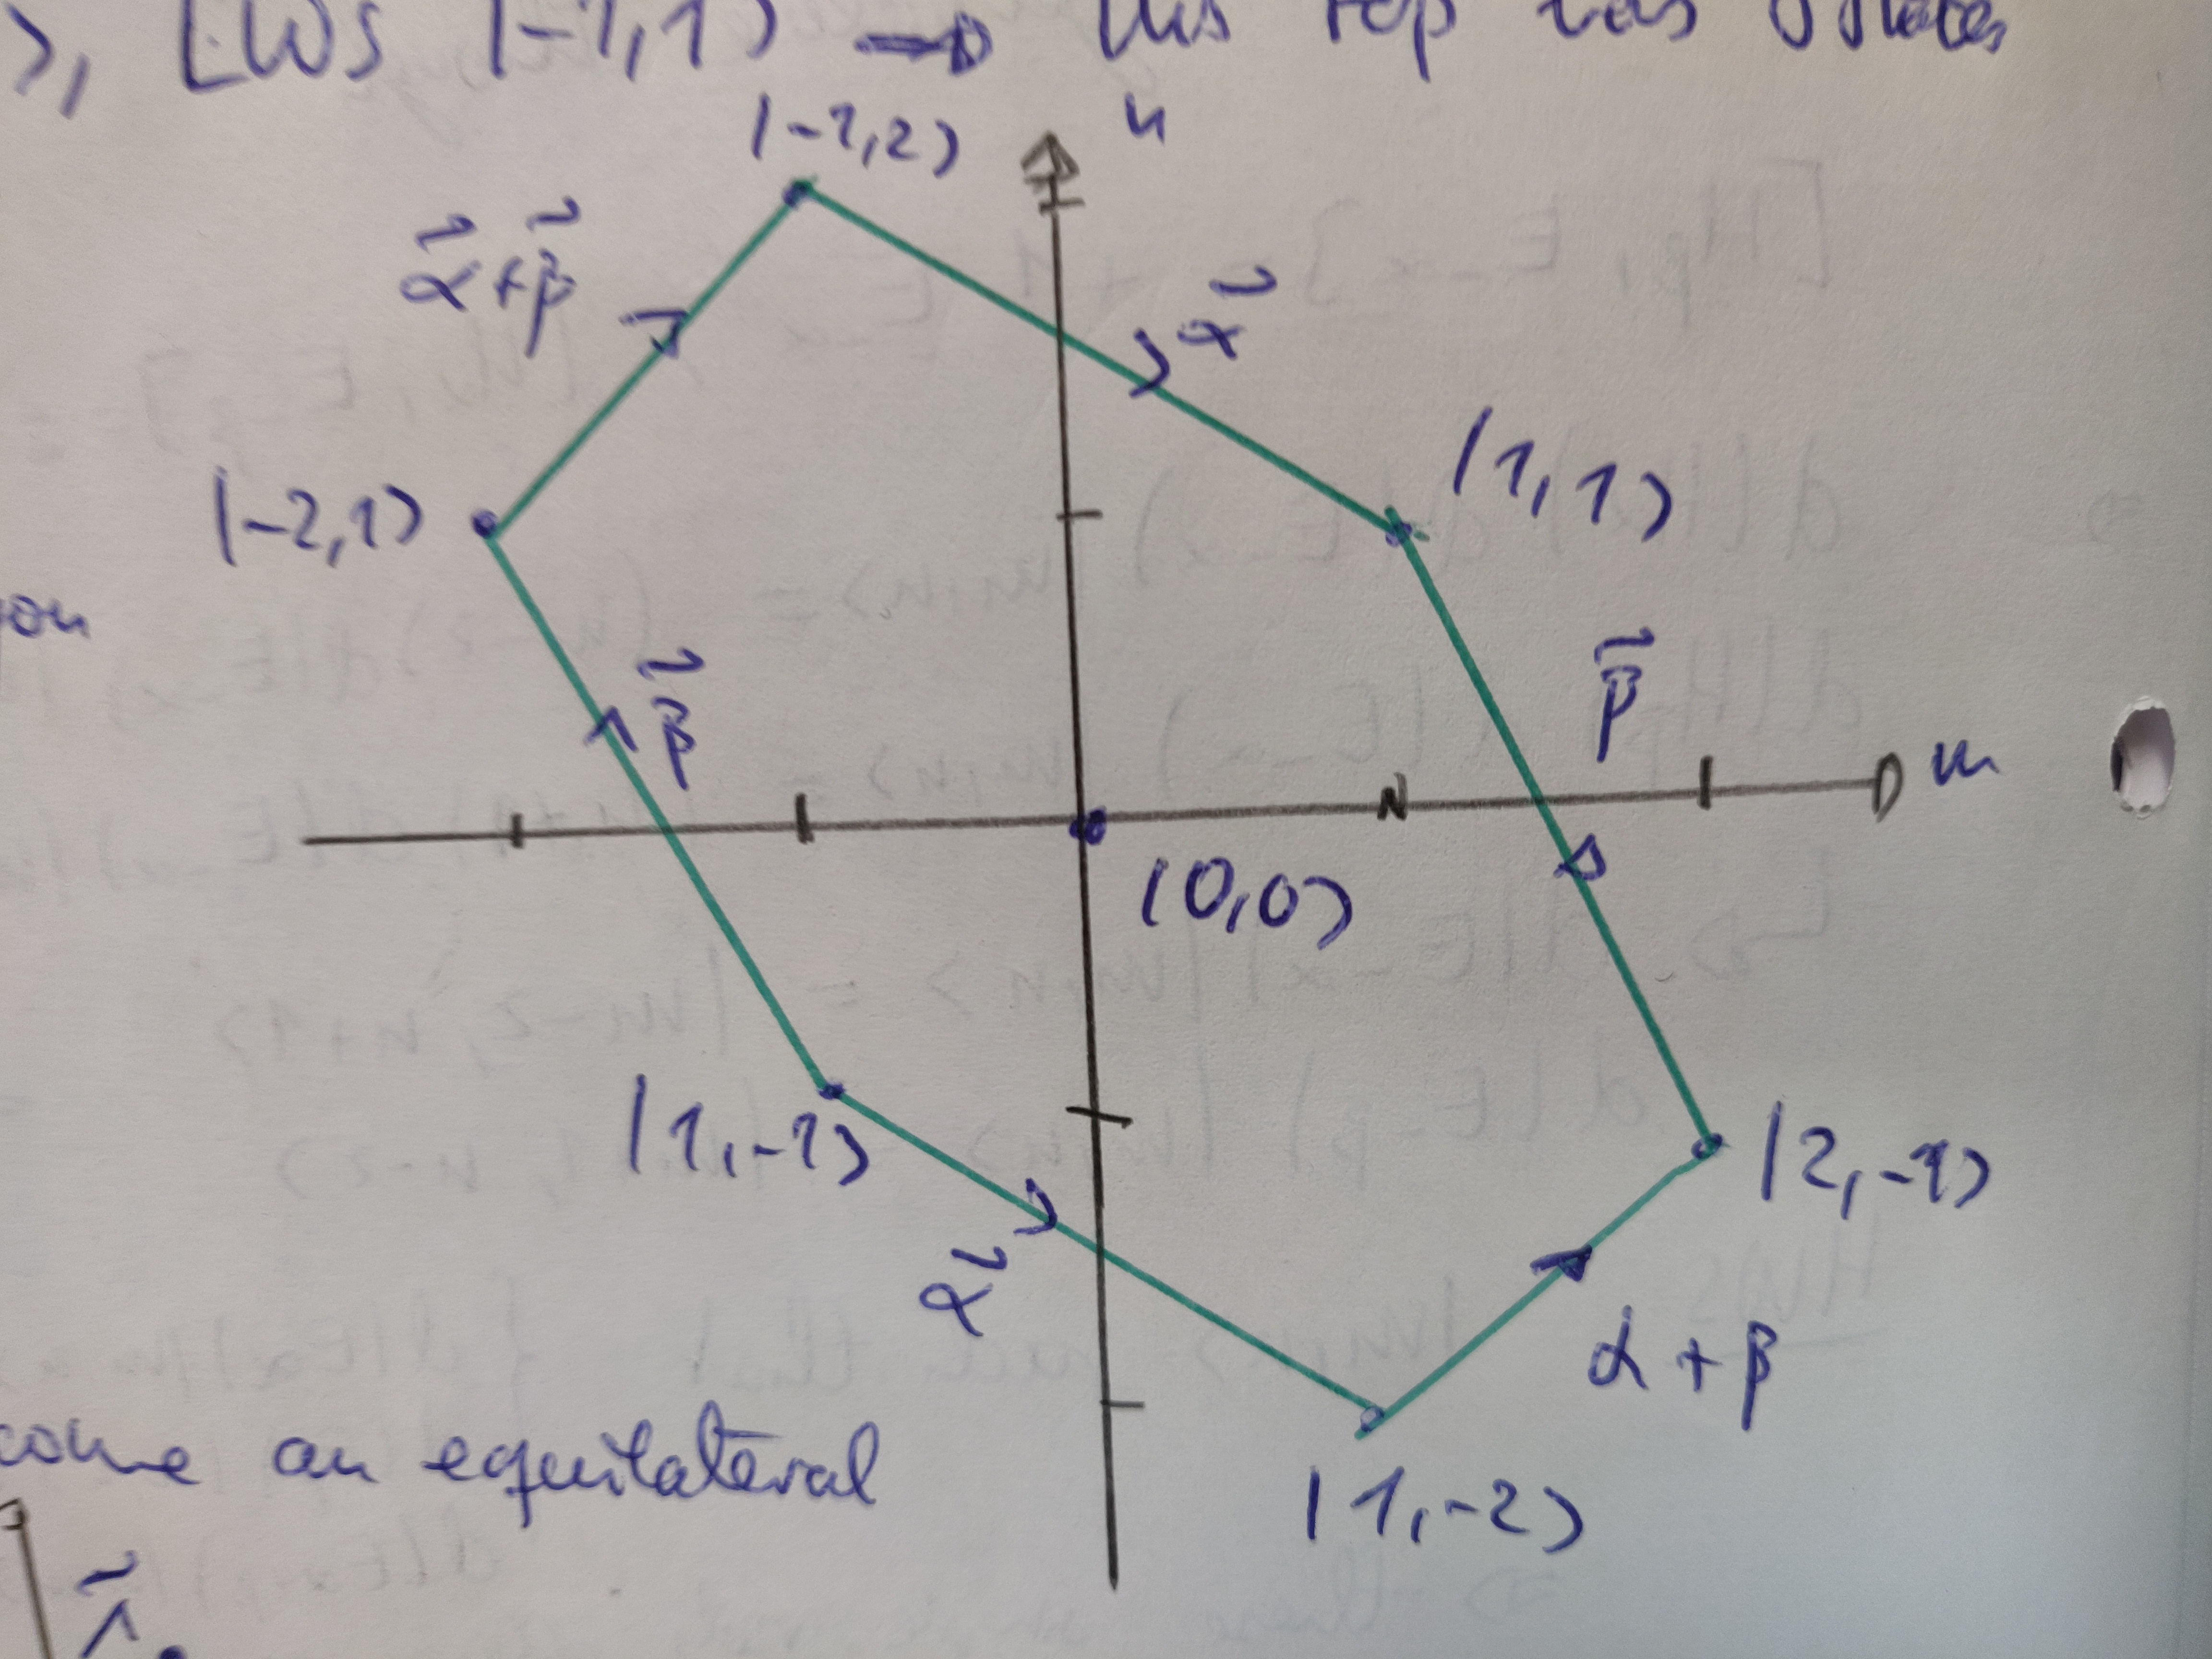
\includegraphics[width=0.5\linewidth]{gfx/squashedhexagon}
	\caption{}
	\label{fig:squashedhexagon}
\end{figure}
such that there is a non-trivial metric on this space of weights.
\\
Under a change of basis, the metric becomes standard Euclidean and in these coordinates we have the $\yng(2,1)$ rep becoming regular hexagon denoting $\Lambda$ as the HWS
\begin{figure}[h!]
	\centering
	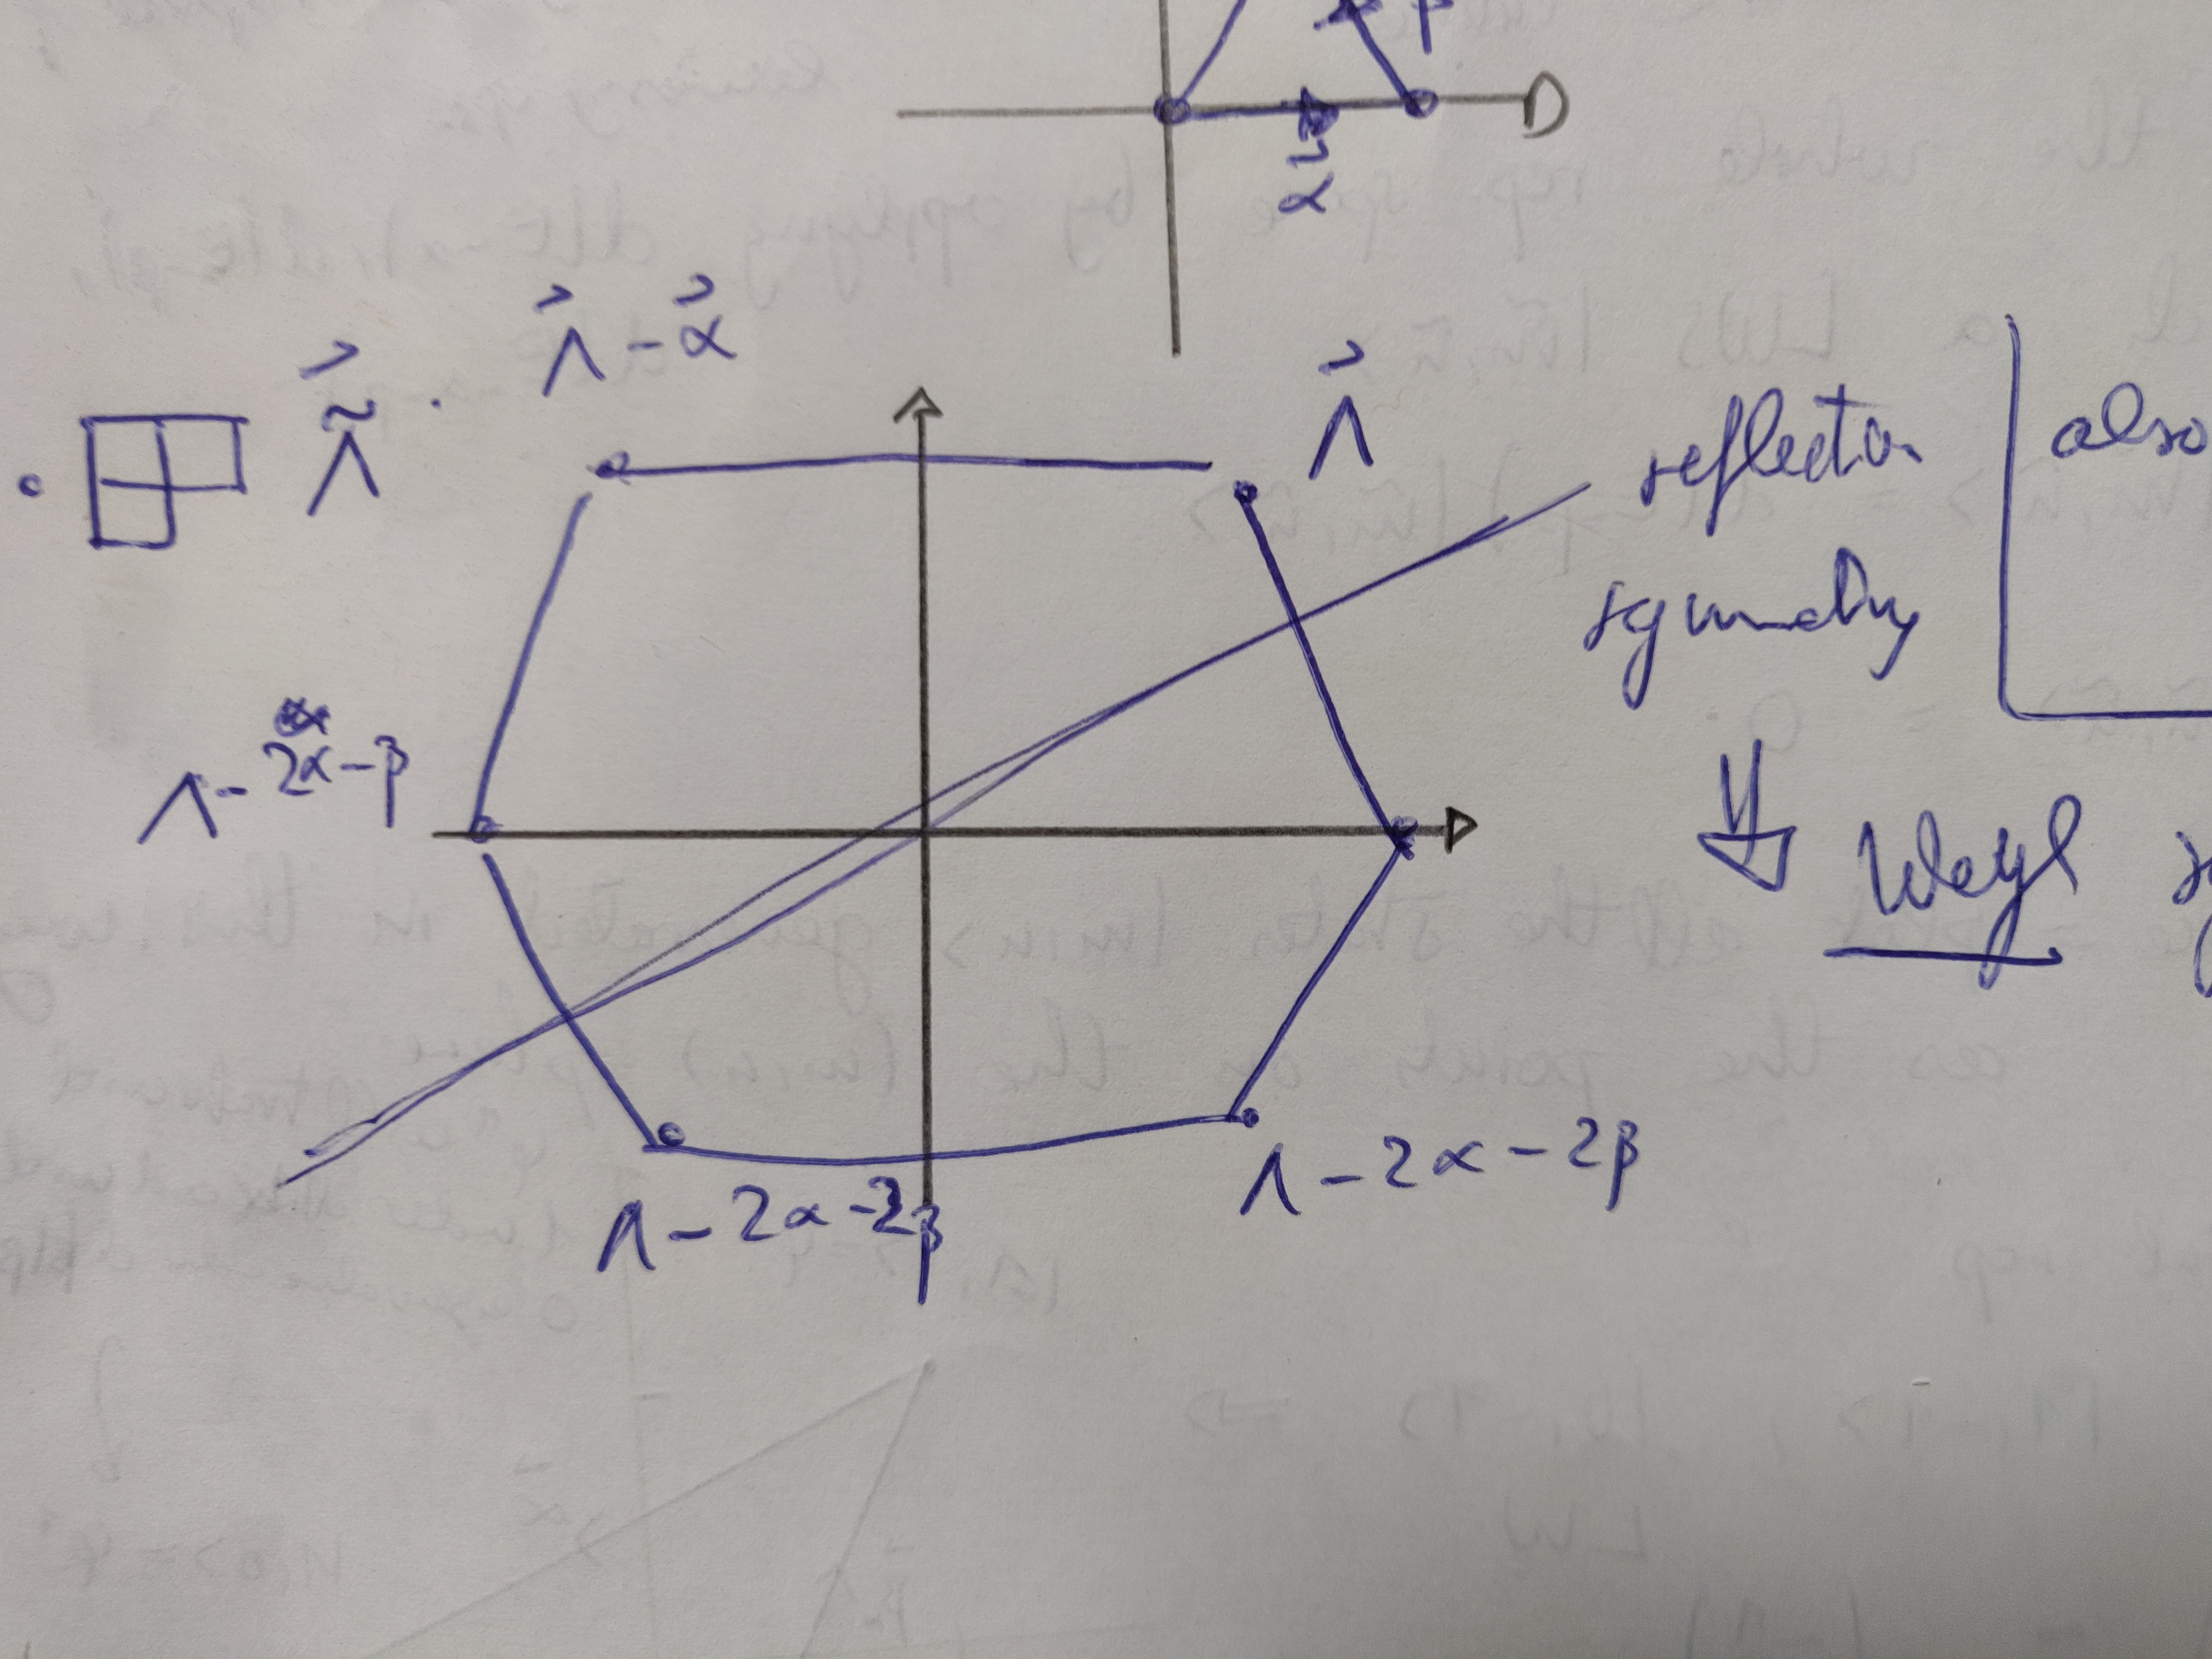
\includegraphics[width=0.5\linewidth]{gfx/weylsymmetrygroups}
	\caption{}
	\label{fig:weylsymmetrygroups}
\end{figure}
\end{enumerate}
\marginpar{General context: $\ket{m,n}$$\leftrightarrow$ Isospin+hypercharge (baryon number+strangeness), two quantum numbers which are conserved in combination (but also independently ?)}
Now for the transition into particle physics, the \emph{Eightfold way} postulated that isospin and strangeness are (actually not) independently conserved, i.e. it represents a symmetry of nature being arranged in irreps of some group falling into $(I_3,s)$ plane. Furthermore, for some spin particle with same baryon number were almost degenerate in mass (Schur's lemma !), one thought that quantum number being conserved (almost in reality) and same mass (almost in reality) one should have a symmetry corresponding to this, the resulting lattice is called the meson octett or the \emph{Eightfold way}.\\
Putting the third component of the isospin on the $x$-axis and the hypercharge (baryon number plus strangeness) on the $y$-axis, i.e. $H_\alpha \leftrightarrow \gamma,H_\beta \leftrightarrow I_3$ one gets
\begin{figure}[h!]
	\centering
	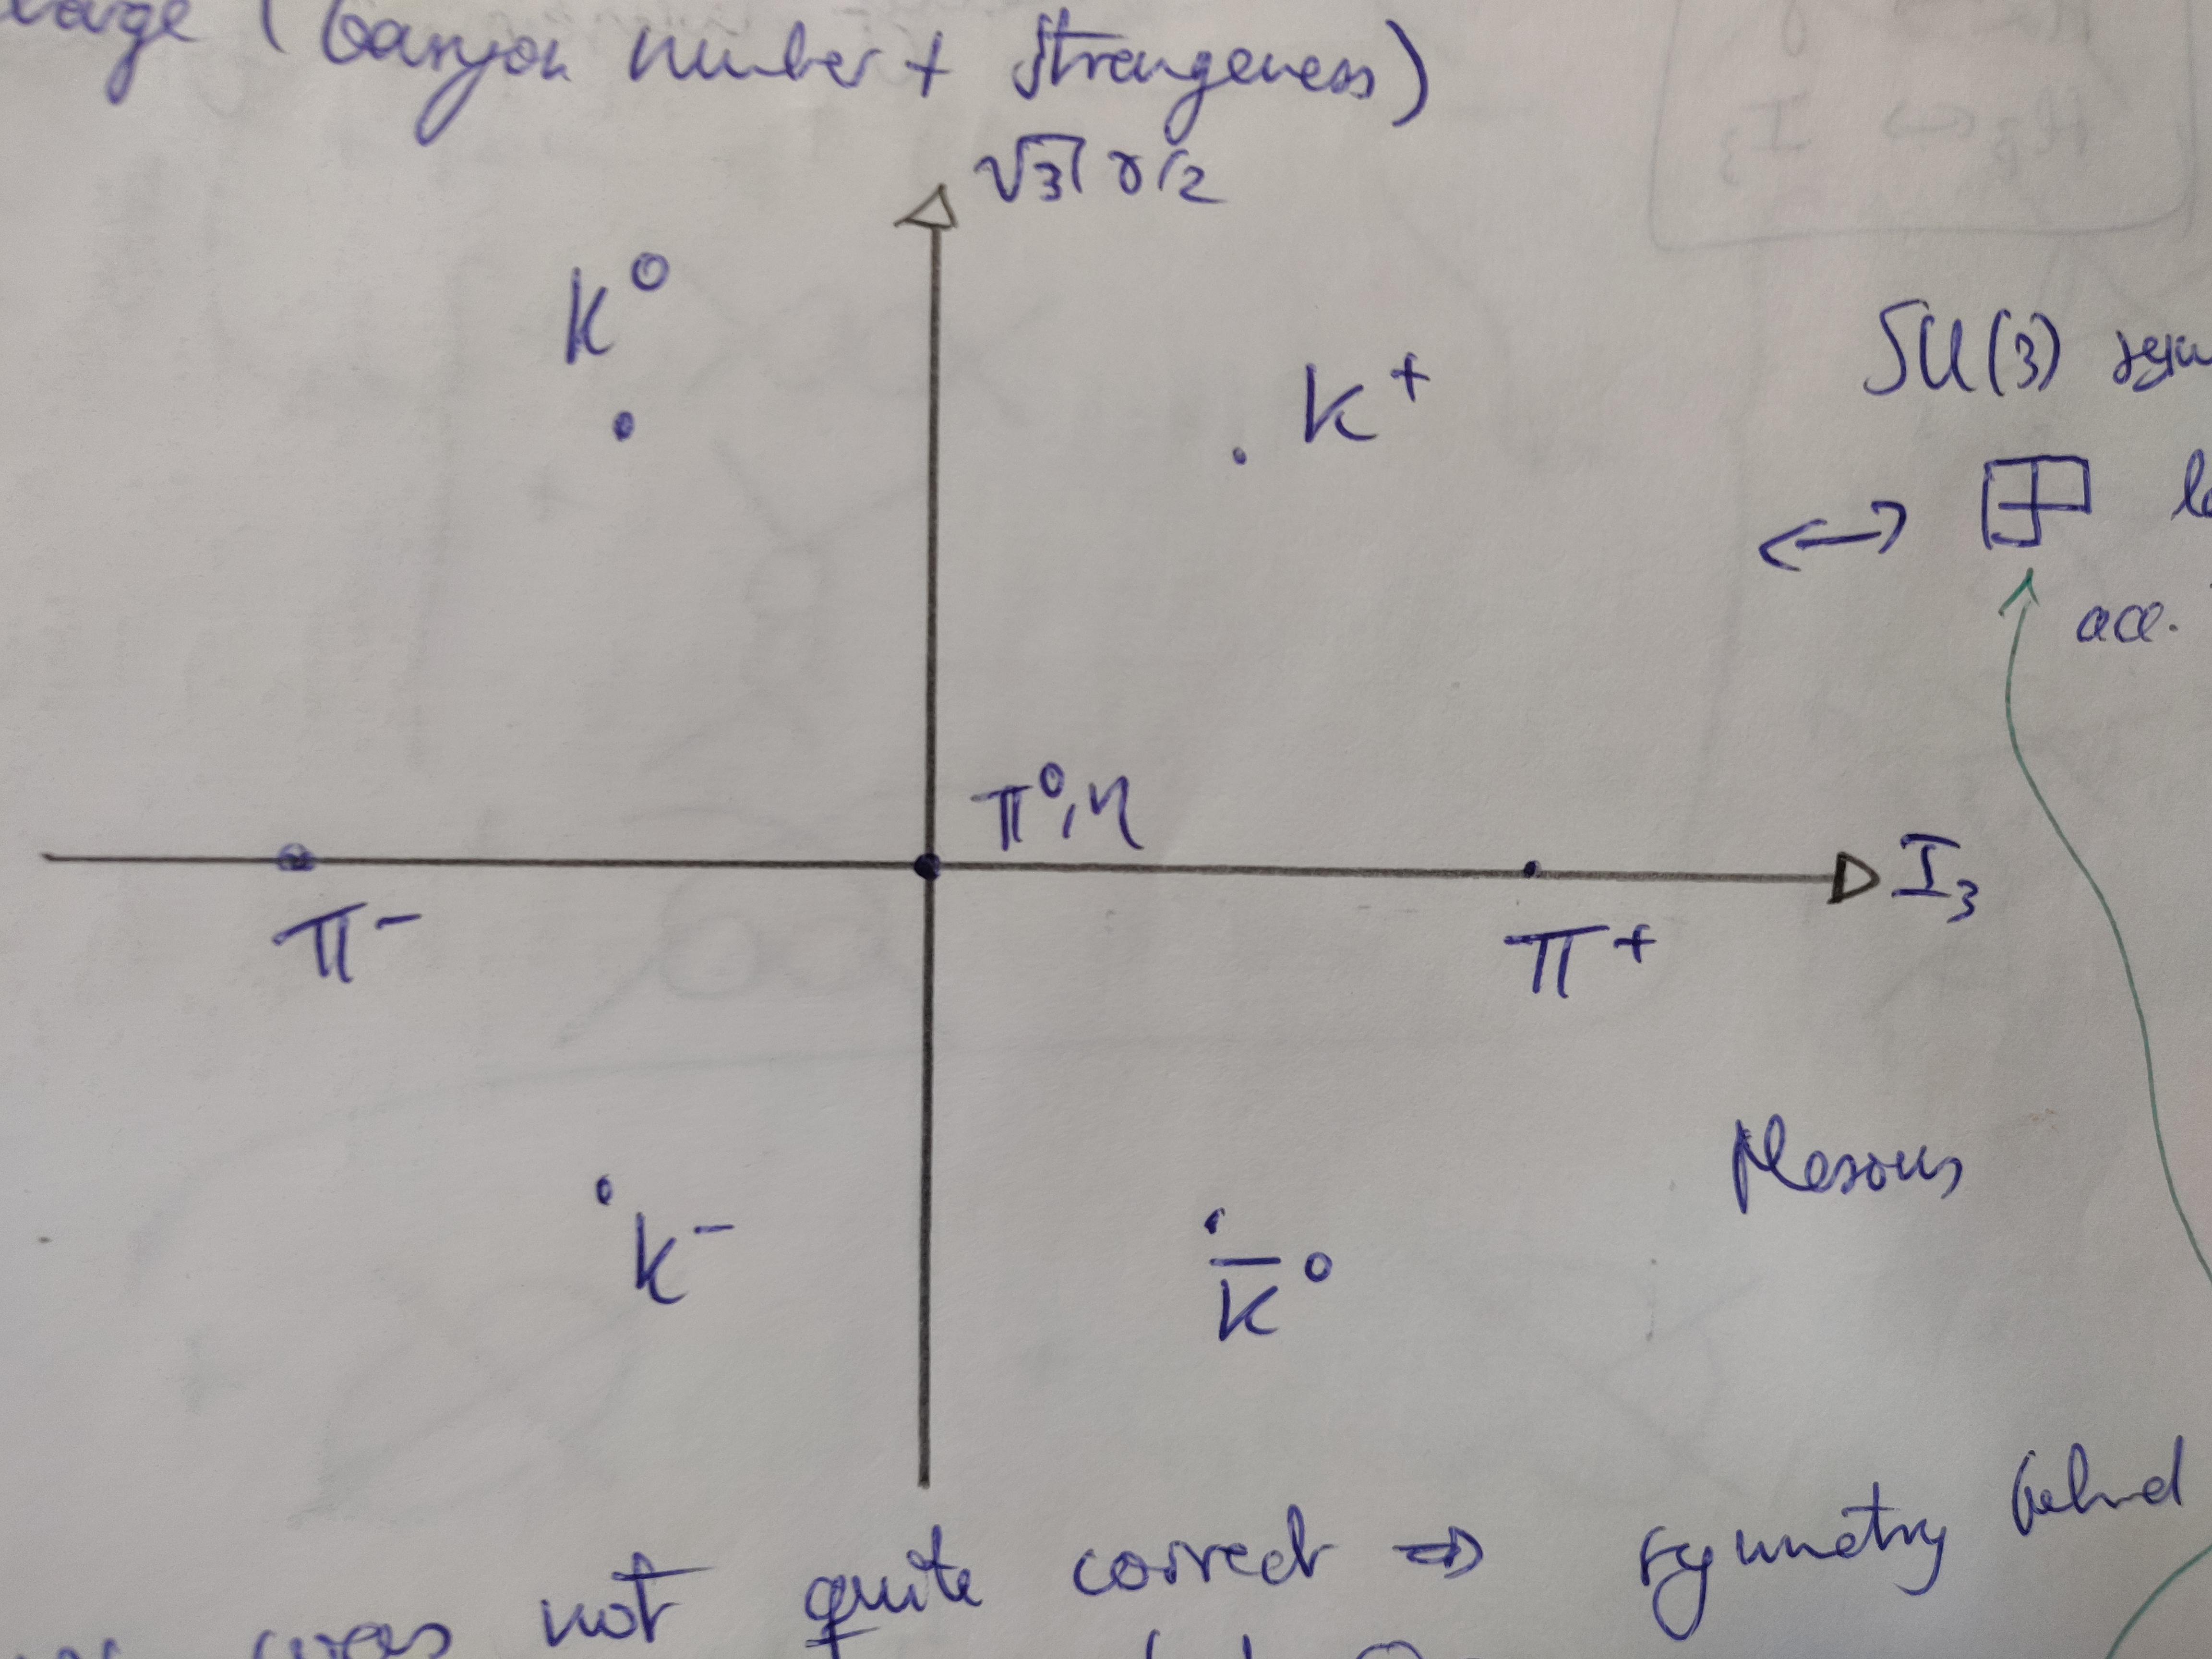
\includegraphics[width=0.7\linewidth]{gfx/eightfoldway}
	\caption{}
	\label{fig:eightfoldway}
\end{figure}
Presumably this corresponds to an $SU(3)$ symmetry, this diagram is equal to $\yng(2,1)$. However, this was not quite correct, the symmetry behind this arrangement wasn't hypercharge or Isospin, but rather QCD.\\
Mesons and Baryons:\\
Idea is that we have quarks $q \leftrightarrow \yng(1)$ transforming in the fundamental representation of $SU(3)$ and anti-quarks $p \leftrightarrow \bar{ \yng(1)}$ transforming in the anti-fundamental rep of $SU(3)$
\begin{align*}
	\text{Meson} &= \yng(1) \otimes \bar{ \yng(1)} = \yng(1) \otimes \yng(1,1) = \yng(2,1) \oplus \mI,\\
	\text{Baryon} &= \yng(1) \otimes \yng(1) \otimes \yng(1) = \yng(3) \oplus \yng(2,1) \oplus \yng(2,1) \oplus \mI \\
	\Leftrightarrow \quad 3\otimes 3\otimes 3&= \underbrace{10}_{\text{baryon decouplet}} \oplus \underbrace{8}_{\text{octett}} \oplus \underbrace{8}_{\text{octett}} \oplus \underbrace{1}_{\text{singlett}}\\
	&=
\end{align*}
\begin{figure}[h!]
	\centering
	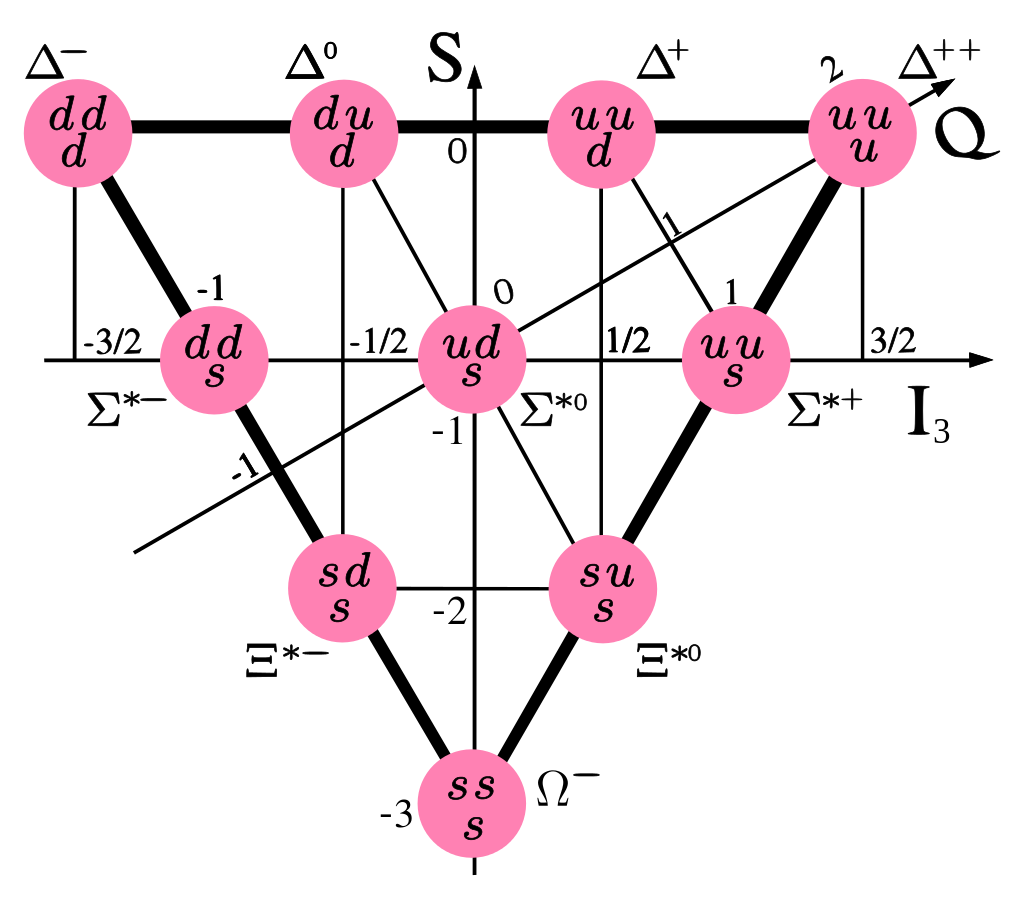
\includegraphics[width=0.5\linewidth]{gfx/Baryon-decuplet}
	\caption{}
	\label{fig:baryon-decuplet}
\end{figure}
note that each of these multiplets have different mass (Schur's lemma) as the symmetry is not really conserved.












\subsubsection{Connection of representation of Lie group at the example of $so(1,3)$ as in the chapter before}
The general idea is:\\
We have a Lie group, e.g. $SO(1,3)$, representing some property/symmetry (eg. spin) or our system, then the objects of our systems (i.e. particles) which have this property (i.e. $s=\half,1,\dots$) transform under irreducible representations of this group (scalar, vector/fundamental, pseudoscalar,pseudovector, tensor,\dots) where the irreducible representations are built via a combination from the generators of the corresponding Lie algebra, i.w. the $4\times 4$ generators $J^{\mu \nu}$ of $so(3,1)$.\\
\\

Consider the relation between matrix groups and Lie algebras: The map "exp" is a diffeomorphism of a small neighbourhood of $O \& \mathcal{I}$ in $M_{n\times n}(\mR)$ and $GL(n,\mR): \exp(a)=g,\exp(0)=\mathcal{I}$.\\
Lie($G$) is the linear subspace of $M_{n\times n}(\mR)$ generated by $exp^{-1}(O_{\mathcal{I}} )$, where $O_{\mathcal{I}}$ is a neighbourhood of $\mathcal{I}\in G \subset M_{n\times n}(\mR)$, compare \ref{fig:liegroups}. 
\marginpar{E.g. $G=SO(3)$, Lie(G)=$\{antisymmetric \, 3\times 3\, matrices\} \Rightarrow$ If $R=\exp(T)$, then $RR^T=e^T(e^T)^T =e^T e^{-T} = \mathcal{I}$.}
\begin{figure}
	\centering
	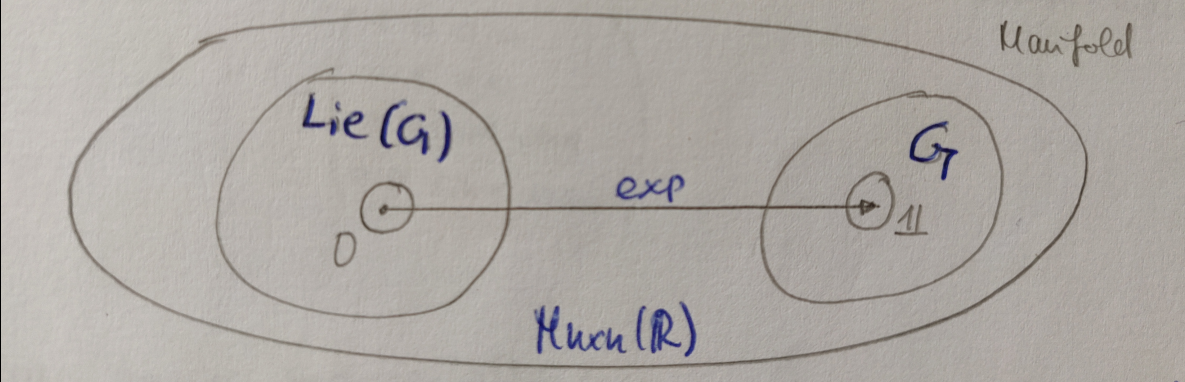
\includegraphics[width=0.7\linewidth]{gfx/Liegroups}
	\caption{\itshape Lie groups relation.}
	\label{fig:liegroups}
\end{figure}
$\Rightarrow exp(a)=g, a\in Lie(G), g\in G$ maps a small neighbourhood/patch of Lie(G) near $O$ to a small patch of $G$ near $\mathcal{I}$. If $a,b \in Lie(G)$, then 
$\exp([a,b])\in G$.
\begin{mybox}{Representation of a Lie-algebra}	
	\begin{equation}
	Lie(G) \stackrel{R}{\rightarrow} M(n), \quad a\mapsto R(a),
	\end{equation}
	with
	\begin{equation}
	R(0)=0, R([a,b])=R(a)R(b) -R(b)R(a) = [R(a),R(b)].
	\end{equation}
	Crucial:\\
	Given some representation $R$ of Lie-algebra Lie(G), we can always construct an associated representation of G (we call it also R) such that
	\begin{equation}
	R(A) = exp(R(a)) \quad if\quad A=\exp(a).
	\end{equation}
	Thus by having a representation of an element of Lie(G) 
	\begin{equation}
	w \, \Rightarrow \, w^{\nu} _{\mu}= -i \half \Omega_{\rho \sigma} (J^{\rho \sigma} )^{\nu}_{\mu} 
	\end{equation}
	we find a representation for an element of G
	\begin{equation}
	\Lambda^{\nu}_{\mu} =\left[\exp(-i \half \Omega_{\rho \sigma} (M^{\rho \sigma} ))\right]^{\mu}_{\nu}.
	\end{equation}
\end{mybox}
Consider $(J^{\rho \sigma})^{\nu}_{\mu}$ as the \emph{canonical basis} of so(1,3), thus these are the antisymmetric generators of SO(1,3). For $\Lambda \in SO(1,3)$ we find a $\tilde{\omega}$ such that we have a representation
\begin{align}
	\Lambda &= e^{\tilde{\omega}} \rightarrow \; \Lambda^{\;\nu}_{\mu} = \delta^{\nu}_{\mu} + \omega^{\nu}_{\mu} \\
	\omega^{\nu}_{\mu} &= -i \half \Omega_{\rho \sigma} (J^{\rho \sigma})^{\nu}_{\mu}.
\end{align}

\section{Lorentz group $SO(3,1)$ structure and Poincaré group}
\subsection{Lorentz group structure}
\begin{mybox}{Proper Lorentz group}
	The set of proper (Lorentz trafo is called proper if $\det\Lambda=1$ holds for its representation), orthochronous (Lorentz trafo is called orthochronous if $\Lambda^0_0 \geq 1$ holds true for its representation) Lorentz transformations makes up the six dimensional Lorentz group
	\begin{equation}
	\label{eq:lorentzgroup}
	L^\uparrow_+ :=\left\{	\Lambda| \eta\munu\Lambda^\mu_{\;\rho} \Lambda^\nu_{\;\sigma} = \eta_{\rho \sigma}, \; \Lambda^0_0 \geq 1,\; \det(\Lambda)=1\right\}.
	\end{equation}
	Note that 
	\begin{equation}
		L^\uparrow_+ = SO(3,1).
	\end{equation}
	It is a subgroup of the Lorentzgroup of which every element is countinously expandable from $\Lambda=\mI$.
\end{mybox}
Equivalent notations of the equation in \ref{eq:lorentzgroup} are
\begin{align}
	\Lambda^{\mu \rho} \Lambda_{\mu \sigma} &= \delta^\rho_\sigma \\
	\Lambda^{\;\rho}_\mu \Lambda^\mu_{\;\sigma} &= \eta^\rho_\sigma.
\end{align}
\begin{mybox}{Poincaré group}
	The Poincarégroup $\mathcal{P}$ and the Lorentz group $L$ are made up of $L^\uparrow_+$, parity transformations $P$, time inversion $T$ and the translations $T_4$ in $\mathbb{M}^4$:
	\begin{equation}
	\label{eq:lorentzgroupwhole}
	L = L^\uparrow_+ \oplus T \oplus P,
	\end{equation}
	\begin{equation}
	\label{eq:poincaregroup}
	\mathcal{P}=L^\uparrow_+ \oplus T_4.
	\end{equation}
\end{mybox}

\subsection{Principle of relativity in the Lagrangian formalism }
\begin{mybox}{Principle of relativity take two}
	In order to obtain equations of motion whose form is the same for all observers, we demand:
	\begin{equation}
	\mathrm{The\, Lagrangian \; \mL \;of \;a \;relativistic\; FT\; is\; invariant \;under \;\mathcal{P}^\uparrow_+}.
		\end{equation}
		Equations that are form invariant are called \emph{covariant}.
	\end{mybox}
	Note the restriction to $\mathcal{P}^\uparrow_+$. Always keep this restriction in mind when reading ’Lorentz invariance’.
	\\
	\\
	This postulate immediately guarantees that the Euler-Lagrange equations are Lorentz covariant
	and that quantities derived from L in a covariant way are Lorentztensors.
	In anticipation of the standard model it should be noted that nature really is not described by a
	Lagrangian that is invariant under parity or timeinversion transformations and we will use terms
	violating P and T when building our SM Lagrangian so excluding those here is really necessary.
\subsection{Generators of boosts and rotations in Minkowski space}

























\subsection{Representation of the Lorentz group}
We want a theory satisfying SRT, this is only satisfied if all fields transform in an irrep of the Lorentz group. Then we will have to study different types of reps (scalar, vector, spinor,\dots) and look at their Noether current wrt. spatial rotation, which has orbital and spin contributions, from which we can read off which spin corresponds to which representation. Thus, \textbf{spin is an afterthought, not an input for the theory}. First we study reps and then afterwards we can make the identification with particles and spin.\\
\\
Relativistic fields are classified by their behaviour under Lorentz transformations, i.e a general transformation
\begin{equation}
	D(\Lambda): \varphi(x) \rightarrow \varphi^\prime (x^\prime) = D(\Lambda) \circ \varphi(x),
\end{equation}
where $D(\Lambda)$ is a particular representation of the element $\Lambda$ of the Lorentz group and where the Lorentz four-vector transforms in a particular representation, namely the vector representation
\begin{equation}
x^{\mu} \mapsto x^{' \mu} = \Lambda^{\mu}_{\nu} x^{¸\nu}, \quad \Lambda^{\mu}_{\nu} \in SO(1,3).
\end{equation}
Generally a field $\phi^a(x)$ transforms then as a representation of the \emph{Lorentz group} $SO(1,3)$. With the field being a map
\begin{equation}
\phi^a :\mR^{1,3} \rightarrow V, x\mapsto \phi^a(x), \; a=1,\dots, \dim V=n
\end{equation}
we have
\begin{equation}
\phi^a(x) \mapsto \phi^{'a} (x) = D(\Lambda)^a_b \phi^b (\Lambda^{-1} x') = D(\Lambda)^a_b \phi^b(x)
\end{equation}
with $D(\Lambda)$ being the representation for $\Lambda \in SO(1,3)$.
\subsubsection{Collection of the different representations of the Lorentz group - a physical approach}
\begin{enumerate}
	\item \emph{Scalar representation}:\\
	
		For a real/complex scalar ($s=0$) field $\phi(x)$, the representation is trivial 
	\begin{equation}
	D(\Lambda) = \mathcal{I} \quad \forall \Lambda \; \Rightarrow \phi'(x')=\phi(x).
	\end{equation}
	This representation only has one dof., it turns out to describe (via angular momentum Noether current) bosons of spin $s=0$.
	\item \emph{Vector representation}:\\
		A vector field ($s=1$) $A^{\mu}(x)$ transforms in the \emph{vector representation} 
	\begin{equation}
	D(\Lambda) = \Lambda^{\;\nu}_{\mu} \quad \forall \Lambda \; \Rightarrow A_{\mu}(x)\rightarrow A^\prime_\mu(x^\prime) = \Lambda^{\;\nu}_\mu \underbrace{A^{\nu}(\Lambda^{-1}x' )}_{=A^\nu(x)}.
	\end{equation}
	From the angular momentum Noether current we know that the Vector rep describes spin $1$ particles (and anti-particles). Spin $1$ has $3$ polarizations ($-1,0,1$), i.e. one longitudinal and two transvere degrees of freedom.\footnote{You can combine the transverse polarizations $T_{1,2}$ to $T_1\pm i T_2$ to describe left-and right-handed polarizations.} Thus, for a vector we do expect $4$ degrees of freedom, but it has $\mu=0,1,2,3 \Rightarrow 4$. The one redundant degree of freedom is fixed by the gauge (as vector fields are gauge fields). Gauge fields have unphysical degrees of freedom corresponding to gauge transformations which can be removed by fixing the gauge transformation. Thus, there is another symmetry beside the Lorentz symmetry in this system under which the vector gauge fields transform, namely the \emph{gauge symmetry}. Gauge fixing, e.g. $\partial_\mu A^\mu=0$, $A_0=0$, removes one dof. such that only $3$ survive.\\
	 However, the photon field only has $2$ polarizations, what happens with the $3$rd ? It decouples. Unbroken gauge invariance (like QED) implies that $m_{\text{gauge field}}=0$, a \textbf{mass term would break gauge invariance}. Whenever $m_{A_\mu}=0$, then the longitudinal polarization decouples, only two dof $\gamma^\pm$ are left, namely the $2$ transverse polarizations.\\
	 Examples of Vector theories:\\
	 \begin{enumerate} 
	 \item Thus, QED is a $U(1)$ gauge theory, the vector field $A_\mu$ gives rise to photons $\gamma$ with $+,-$ transverse polarizations only and $m_\gamma=0$.\todo{Reference to this theory}
	 \item QCD is a $SU(3)$ gauge theory, the vector field $A^{a=1,\dots,8}_\mu$ are $8$ gluon fields (as $SU(3)$ has $8$ generators) $g^{1\dots 8}$ which are also massless, because it has an exact gauge symmetry, $m_g=0$ with two polarizations.\todo{Reference to this theory}
	 \item Weak interactions are described by $SU(2)_L$ gauge theory (Glashow-Weinberg-Salam), the weak interaction sector of the standard model. $SU(2)$ has $3$ generators, which implies that there exist $3$ vector fields $A^{a=1,2,3}_\mu$ which actually are the $3$ weak vector bosons $W^+,W^-,Z^0$ \todo{reference to this theory}. However, these \emph{are massive} $m_{W^\pm}\neq 0, m_{Z^0}\neq 0$, because the $SU(2)$ gauge symmetry is spontaneously broken by the Higgs mechanism. Thus, there are $3$ spin polarizations for each $W^+,W^-,Z^0$, i.e. $1$ longitudinal $L$ and two transverse $+,-$.
	 \end{enumerate}
 \item \emph{Tensor representation}:\\
 A rank $(0,2)$ tensor transforms according to 
 \begin{equation}
 T\munu(x) \rightarrow T^\prime\munu(x^\prime) = \Lambda^{\;\rho}_\mu \Lambda^{\;\sigma}_\nu T_{\rho \sigma}(x).
 \end{equation}
 Rank $(0,2)$ tensors are however reducible, they decompose into two irreps, i.e. the \emph{symmetric} and \emph{anti-symmetric} irrep. Whilst the symmetric tensor irrep describes spin $2$ particles like the graviton, the antisymmetric tensor irrep does not describe any new particles as it can be constructed from vectors, consider for example the field strength $F\munu =\partial_\mu A_\nu - \partial_\nu A_\mu$, i.e. not an independent degree of freedom.\\
 \\
 \textbf{Renormalizability of QFT} is the essential requirement which confines our interest to the scalar, vector and spinor representation, as e.g. the symmetric $2$ tensor rep represents a non-renormalizable theory, i.e. gravity.
 \item \emph{Lowest spinor representation}:\\
 A spinor like the Dirac fermion/spinor field $\psi_D(x)$, which is a four-component complex-valued spinor, transforms in the spinor representation
 \begin{equation}
 	D(\Lambda) = S \in M^{4 \times 4}, \; S=S(\gamma^\mu) \Rightarrow \; S\circ \psi_D(x).
 \end{equation}
 A (Dirac) spinor is not a vector as it does \emph{not} transform like a vector but like a spinor (i.e. $4\pi$ rotation to identity).\\
 It is a reducible rep made up out of $2$ irreps
 \begin{enumerate}
 	\item $\psi^{\alpha=1,2}_L$ is the left-handed irrep for the \emph{Weyl spinor}, which is a $2$-component spinor $\alpha=1,2$.
 	\item $\psi_{R,\dot{\alpha}=1,2}$ is the right-handed irrep for the Weyl spinor, which is a $2$-component spinor $\dot{\alpha}=1,2$
 \end{enumerate}
In the \emph{Chiral basis} for $\gamma^\mu$, i.e. 
\begin{equation*}
	\gamma^\mu = \begin{pmatrix}
	0&\sigma^\mu \\ 
	\bar{ \sigma}^\mu &0\\
	\end{pmatrix}, \quad \sigma^\mu =(\mI,\vec{\sigma}), \quad \bar{ \sigma }^\mu =(\mI,-\vec{\sigma}),
\end{equation*}
the Dirac spinor decomposes into the two Weyl spinors
\begin{equation}
\psi_D(\begin{pmatrix}
\psi^\alpha_L\\ \psi_{R,\dot{\alpha}} \\
\end{pmatrix})
= \begin{pmatrix}
\psi^1_L\\
\psi^2_L\\
\psi_{R,\dot{1}} \\
\psi_{R,\dot{2}} \\
\end{pmatrix}
\end{equation}
where the respective indices of the disjoint subspaces $(\sigma^\mu)^{\alpha \dot{\alpha}}$, $(\bar{ \sigma }^\mu)_{\dot{\alpha}\alpha}$, $\;\alpha,\dot{\alpha}=1,2$ are raised and lowered with $\epsilon$ tensors $\epsilon^{\alpha \beta}, \epsilon_{\dot{\alpha}\dot{\beta}}$ respectively.\\
\\
Note that there are also LH and RH electrons which we group into the Dirac electro ($\leftrightarrow\psi_D$) as they interact the same way with photons and gluons. However, they interact differently with $W^\pm$. Thus, the electron as an elementary particle is not corresponding to a reducible rep, i.e. $\psi_D$, but really corresponds to the $2$ irreducible Weyl spinor $e^-_L,e^-_R$.\\
$\psi_L$ describes LH chiral fermions (i.e. chirality is $+\half$) whereas $\psi_R$ describes RH chiral fermions with chirality $-\half$. They do transform differently under $SO(1,3)$ where they have different signs in the boost \ref{subsubsec:lhrhSpinors}.
\end{enumerate} 


\subsubsection{Representations of the Lorentz group, again but more thoroughly - a mathematical approach}
With a change of basis from the separate generators of boosts $K^i$ and of rotations $J^i$ to $N_i = \half (J_i -i K_i),\bar{ N}_i=\half (J_i +i K_i)$, we get two disjoint copies of $su(2)$, namely $su(3)=su(2)_L \times su(2)_R = (\half,0) \oplus (0,\half)$ which, provided their irreps, give us the irreps of the Lorentz group. We know the irreps of $su(2)$, i.e. $\cdot=\mI,\yng(1),\yng(2),\dots$ We just need an integer $j\in \mathbb{N}$ to specify an $su(2)$ irrep, i.e. for $so(3,1)$ we need two integers:\\
Any $SO(3,1)$ irreps $(j_1,j_2)\rightarrow(SU(2)_L,SU(2)_R)$ has dimension
\begin{equation*}
\dim(j_1,j_2) = (j_1+1)\cdot (j_2+1)
\end{equation*}
\marginpar{The physics convention is always a half of the value}
\begin{enumerate}
\item[$(0,0)$] \emph{Trivial representation}, the scalar field $\phi$
\item[$(1,0)=(\half,0)$] \emph{Left-handed Weyl spinor} $\psi_\alpha$ ($\alpha=1,2$) which transforms in the fundamental representation of $su(2)_L$ and in the trivial rep of $su(2)_R$
\item[$(0,1)=(0,\half)$] \emph{Right-handed Weyl spinor} $\bar{ \psi}_{\dot{\alpha}}$ ($\dot{\alpha}=1,2$) which trafos as trivial rep of $su(2)_L$ and in the fundamental rep of $su(2)_R$.
\item[i)] Note that the Dirac spinor itself is not an irreducible representation but a composite of two irreducible reps, namely the left-and right-handed Weyl spinors
\begin{equation*}
	\text{Dirac spinor} = (1,0) \oplus (0,1) = (\half,0) \oplus (0,\half) \text{ latter is physics convention}
\end{equation*}
\item[$(1,1)=(\half,\half)$] \emph{Vector representation} for $A_\mu$, which transforms in the fundamental rep of $SU(2)_L\&SU(2)_R$.\\
How do we get to the vector representation $A_\mu$ when it should actually be $A_{\alpha \dot{\alpha}}$ ? Via repackaging:\\
Note that the dimensions are $\dim(1,1)=2\cdot 2=4$, i.e. a $4$-component vector, and that $\dim(1,0)=\dim(0,1)=2$, i.e. $A_{\alpha \dot{\alpha}}$ is a $2\times2$ matrix with $4$ components.
\item[$(2,0)=(1,0)$] \emph{Self-dual $2$-form} which is given by $F_{(\alpha \beta)}$, by repackaging one has eg. objects $F\munu= \half \epsilon{\munu \rho \sigma} F^{\rho \sigma}$, with $F_[\mu \nu], F=*F$, which is what one calls an \emph{instanton}.
\item[$(0,2)=(0,1)$] \emph{Anti-self-dual $2$-form} which is given by $B_{\dot{\alpha}\dot{\beta}}$, by repackaging one has eg. objects $B\munu= - \half \epsilon_{\mu \nu\rho \sigma} B^{\rho \sigma}$ with $B=-*B$, which is what one calls an \emph{anti-instanton}.
\end{enumerate}
The Dirac spinor is a \emph{reducible representation} since it is a composite of two irreducible reps
\begin{equation*}
(1,0) \oplus (0,1) \leftrightarrow 	\psi_D= \begin{pmatrix}
		\psi_\alpha\\
		\bar{ \psi}_{\dot{\alpha}}\\
	\end{pmatrix}\;\Rightarrow\; \dim\left[(1,0)\oplus (0,1) \right] = 4.
\end{equation*}
This object allows you two write down a mass term $\propto \bar{ \psi}\psi$, which due to the Weyl symmetry would not be possible for the separated Weyl-spinors.\\
\subsubsection{A comment on Left-handed vs Right-handed Weyl Spinors}
\label{subsubsec:lhrhSpinors}
\begin{enumerate} 
	\item[LH]
As described above, the LH Weyl spinor $(1,0)$ transforms in fundamental rep $\yng(1)$ of $SU(2)_L$ and in the trivial rep $\mI$ of $SU(2)_R$, i.e.
\begin{equation*}
	(1,0)=\yng(1)_L \times \mI_R.
\end{equation*}
Thus, the generators of $SU(2)_L$ must be represented in fund rep: $\md(N_i)=-\half \sigma_i$, whereas the generators of $SU(2)_R$ must be represented in scalar rep $\md(\bar{ N}_i)=0$. \\
Consider the group action of the LH spinor by considering one group element of $SO(3,1)$, $\Lambda^\mu_{\;\nu}=\exp(\omega^\mu_{\;\nu}), \omega^\mu_\nu$ has $6=r_i+b_i=3+3$ parameters, $3$ rotations $r_i$ and $3$ boosts $b_i$
\begin{equation*}
	D(\Lambda): \psi_\alpha \rightarrow \exp(\underbrace{n_i}_{Ar_i+Bn_i} \md(N_i))^\beta_\alpha \psi_\beta = \underbrace{\exp(-\frac{i}{2} r_i \sigma_i \textcolor{red}{-} \frac{b_i}{2}\sigma_i)^\beta_\alpha}_{M^\beta_\alpha}\psi_\beta
\end{equation*}
which is \emph{not} a unitary irreps, since $\sigma_i b_i$ is not a unitary matrix as $\sigma_i$ is only hermitian. Therefore $M^\beta_\alpha \in SL(2,\mathbb{C})$, which is the complexification of $SU(2)$. $SO(3,1)$ is a non-compact group since boost never reach $c$, only $v<c$ is allowed. If you picture Lie groups as manifolds, then the Lorentz group is not spherical but rather hyperbolically formed as $\beta \in (-1,1)$ such that the manifold is non-compact.\\
We only get a pseudo representation of $SO(3,1)$ as $r_i$ needs $4\pi$ to get back to identity. Therefore, \emph{spinors are just a pseudo-representation}, even though they are composite objects of real irreps.
\item[RH] Transforms in trivial rep of $SU(2)_L, \tilde{\md}(N_i)=0$, and in the fundamental rep of $SU(2)_R, \tilde{\md}( \bar{ N}_i)= - \frac{i\sigma_i}{2}$. Consider the group action under the same group element as above
\begin{align*}
	\tilde{D}(\Lambda)&=\exp\left[-\frac{i}{2} r_i \sigma \textcolor{red}{+} \frac{b_i\sigma_i}{2} \right] = \exp((n_i)^* \tilde{\md}(\bar{ N}_i))\\
	\bar{ \psi}_{\dot{\alpha}} &\rightarrow (M^*)^{\dot{\beta}}_{\dot{\alpha}}   \; \bar{ \psi}_{\dot{\beta}},
\end{align*}
thus RH and LHR spinors trafo the same under rotation (as they are massless, spin does not care about that), but different under boosts (different helicity transformation).
\end{enumerate}
\subsubsection{A comment on how to repackage the vector representation}
Consider the group action of the vector rep $(1,1)\Rightarrow D_V(\Lambda)$:
\begin{equation*}
	D_V(\Lambda) : C_{\alpha \dot{\alpha}} \rightarrow M^{\;\beta}_\alpha (M^*)^{\;\dot{\beta}}_{\dot{\alpha}} C_{\beta \dot{\beta}} = (M C M^\dagger)_{\alpha \dot{\alpha}}
\end{equation*}
which does not look like a vector transformation. Redefine the variables to see it. Introduce $\sigma^\mu=(\mI_{2\times 2}, - \vec{\sigma})$, suppose a vector
\begin{equation*}
	D_V(\Lambda):x^\mu \rightarrow \Lambda^\mu_{\;\nu} x^\nu = x^{\prime \mu},\quad x^\mu \eta\munu \sigma^\nu =\begin{pmatrix}
		x^0+x^3&x^1-ix^2\\
		x^1+ix^2 & x^0-x^3\\
	\end{pmatrix}
=:X_{\alpha \dot{\alpha}},
\end{equation*}
then
\begin{equation*}
X^\prime_{\alpha \dot{\alpha}} = (M X M^\dagger)_{\alpha \dot{\alpha}},
\end{equation*}
where $M$ is the LH and $M^\dagger$ is the RH $2\times 2$ representation of the same $\Lambda \in SO(3,1)$. The packaging may be different, but the info is the same. Just write it as $4$-component vector.




\subsubsection{The Lorentz algebra}
\marginpar{For $V=\mR^{1,3} \Rightarrow a,b \equiv \mu,\nu$}
\marginpar{Find a representation of element of Lie-group $\Lambda \in SO(1,3)$ by having a representation for element of Lie($G$): $R(\Lambda)e^{R(a)}, \, a\in Lie(G)$.}
By a representation of the homogeneous Lorentz group, we mean a set of matrices $D(\Lambda)$ satisfying the group multiplication law 
\begin{equation*}
	D(\bar{ \Lambda}) D(\Lambda) = D(\bar{ \Lambda} \Lambda).
\end{equation*}
Just as for the unitary operators in general group representations, we can study the properties of matrices by considering the infinitesimal case
\begin{equation}
\Lambda^\mu_{\;\nu} = \delta^\mu_\nu + \omega^\mu_\nu,\quad \omega\munu=-\omega_{\nu\mu},
\end{equation}
for which
\begin{equation}
\label{eq:spinortrafo}
D(\Lambda) = 1 + \half i \omega\munu  J^{\mu \nu},\quad J^{\mu \nu} = - J^{\nu \mu} 
\end{equation}
a set of matrices satisfying the commutation relations \ref{eq:commutatorso3}.











\begin{mybox}{Basis of so(1,3)}
	We find six antisymmetric $4\times4$ matrices as elements of the basis of the six-dimensional Lorentz algebra $so(1,3)=Lie(SO(1,3))$
	\begin{equation}
	(J^{\rho  \sigma})^{\mu \nu} = i \left[\eta^{\rho \mu} \eta^{\sigma \nu} - \eta^{\rho \nu} \eta^{\sigma \mu} \right].
	\end{equation}
	The $J^{\rho \sigma}$ are the \emph{generators of the Lie group SO(1,3)}, or equivalently form a \emph{basis of the Lie algebra so(1,3)}. This is the algebra of infinitesimal Lorentz transformations connected to the identity. We find in this basis
	\begin{equation}
	\Lambda^{\mu}_{\nu} = \left[e^{-i \half w_{\rho \sigma }J^{\rho \sigma}  }\right]^{\mu}_{\nu}.
	\end{equation}
	The defining commutator of the Lie-algebra $so(1,3)$ is 
	\begin{equation}
	\label{eq:commutatorso3}
	[J^{\mu \nu}, J^{\rho \sigma} ] = i \left[\eta^{\nu \rho} J^{\mu \sigma} - \eta^{\mu \rho} J^{\nu \sigma} - \eta^{\nu \sigma} J^{\mu \rho} + \eta^{\mu \sigma} J^{\nu \rho}\right].
	\end{equation}
	These six basis elements $(J^{\rho \sigma})^{\mu \nu}$ therefore generate the three boosts and three rotations of the Lorentz group SO(1,3).
\end{mybox}

E.g. Rotation (spatial) by angle $\alpha$ around an axis $\vec{n}$:
\begin{align*}
	\omega_{ij} &= \alpha \epsilon_{ijk} n^k \qquad \vec{n} = (1,0,0)^T\\
	\Rightarrow 	w_{\rho \sigma} &=
	\begin{pmatrix}
		0&0&0&0\\
		0&0&0&0 \\
		0&0&0&\alpha \\
		0&0&-\alpha &0\\
	\end{pmatrix}
	\Rightarrow \; \Lambda^{\mu}_{\nu} = \delta^{\mu}_{¸\nu} + \omega^{\mu}_{\nu} = 
	\begin{pmatrix}
		1 &0&0&0\\
		0&1&0&0 \\
		0&0&1&\alpha \\
		0&0&-\alpha &1 \\
	\end{pmatrix}
\end{align*}
For an infinitesimal rotation $\Lambda^{\mu}_{\nu} \in SO(1,3)$. Thus not infinitesimmaly
\begin{equation}
\Lambda^{\mu}_{\nu} = 
\begin{pmatrix}
1&0&0&0\\
0&1&0&0 \\
0&0& \cos \alpha & -\sin \alpha \\
0&0& \sin\alpha & \cos \alpha
\end{pmatrix}
\end{equation}


  \subsection{The Poincare group and associated Lie algebra}
  \begin{mybox}{Poincaré algebra}
  	The Poincaré algebra is given by
  	\begin{align}
  		[J^{\mu \nu} , J^{\rho \sigma}] &= i \left( \eta^{\nu \rho} J^{\mu \sigma} - \eta^{\mu\rho} J^{\nu\sigma} +\eta^{\mu \sigma} J^{\nu\rho} -\eta^{\nu\sigma} J^{\mu\rho} \right)\\
  		[P^\mu,J^{ \rho \sigma}]&= -i \left(\eta^{\mu \rho} P^\sigma - \eta^{\mu \sigma} P^\rho\right)\\
  		[P^\mu,P^\nu]&=0.
  	\end{align}
  The fundamental representation of the Lorentz group is
  \begin{equation}
  	\Lambda^\mu_{\;\nu} =e^{i \half \omega_{\alpha \beta} (J^{\alpha \beta})^\mu_{\;\nu}}, \quad \mathrm{with}\; (J^{\alpha \beta})^\mu_{\;\nu} = i (\delta^\alpha_\mu \delta^\beta_\nu -\delta^\beta_\mu \delta^\alpha_\nu ).
  \end{equation}
  \end{mybox}
  Note that the commutator relations of the Poincaréalgebra, together with $P^0 ≡ H$, immediately
  imply that momentum, angular momentum, and energy are conserved in the sense of QM
  \begin{equation}
  	[\vec{P},H]=[\vec{J},H] = [H,H] =0.
  \end{equation}
  Note that 
  \begin{equation}
  	J^{\mu\nu}= i(x^\mu \partial^\nu - x^\nu \partial^\mu )
  \end{equation}
  and $(J^{\alpha \beta} )^{\mu\nu}$ is the antisymmetrized metric, i.e.
  \begin{equation}
  (J^{\alpha \beta})^{\mu \nu} = i \eta^{\mu [\alpha}\eta^{\beta]\nu}.
  \end{equation}
¸\subsection{The Dirac spinor representation}
To find such a set of matric $\{J^{\mu\nu}\}$, the basis of $so(1,3)$, we suppose we first construct matrices $\gamma^\mu$ that satisfy the \emph{anti}commutation relations $\{\gamma^\mu, \gamma^\nu \} = 2 \eta^{\mu \nu}$ and tentatively define $J^{\mu \nu} = - \frac{i}{4} [\gamma^\mu,\gamma^\nu]$, which satisfy the desired commutation relations \ref{eq:commutatorso3} via the defining property of the anticommutator. We shall further assume that the matrices $\gamma_\mu$ are irreducible; that is, that there is no proper subspace that is left invariant by all these matrices. Any set of matrices satisfying the anticommutator relation is called a \emph{Clifford algebra}. The importance of this particular representation of the homogeneous Lorentz group (or, more accurately, from its covering group) arises from the fact that the most general irreducible representation of the Lorentz group is either a tensor, or a spinor transforming as in \ref{eq:spinortrafo} with suitable $J^{\mu\nu}$, or a direct product of a spinor and a tensor.




\begin{mybox}{Representation connected to spin }
	Spin $\half$ particles are described by fields in the \emph{spinor representation}.
\end{mybox}
\marginpar{Dirac algebra is a complexification of the real spacetime algebra  $Cliff(1,3,\mR): Cliff(1,3\mathbb{C}) = Cliff(1,3,\mR) \otimes \mathbb{C}$.}
\begin{mybox}{Dirac/Clifford algebra and spinor representation}
	
	Every representation of Cliff(1,3) induces a representation of so(1,3). To find the spinor representation of so(1,3) we start from the Clifford algebra Cliff(1,3) defined as the algebra spanned by $n \times n$-matrices $(\gamma^{\mu})^A_B, \mu=0,1,2,3$ and $A,B=1,\dots,n$ such that the anti-commutator is
	\begin{align}
		\{\gamma^{\mu}, \gamma^{\nu} \} & := 2 \eta^{\mu \nu} \mathcal{I}_{n\times n} \\
		\Rightarrow \gamma^{\mu} \gamma^{\nu} &= 
		\left\{ \begin{array}{lr}
			\eta^{\mu \nu} & if \mu =\nu \\
			- \gamma^{\nu} \gamma^{\mu} & if \mu\neq \nu
		\end{array}		\right\},
		\\
		&(\gamma^0)^2=\mathcal{I},\quad (\gamma^i)^2 = - \mathbf{I}.
	\end{align}
	With the following object 
	\begin{equation}
	(S^{\rho \sigma})^A_B := \frac{i}{4} [\gamma^{\rho},\gamma^{\sigma}]^A_B
	\end{equation}
	we find a basis of so(1,3), i.e.
	\begin{equation}
	[S^{\rho \sigma}, S^{\tau \kappa} ] = -i \left[\eta^{\rho \kappa} S^{\sigma \tau} + \eta^{\sigma \tau} S^{\rho \kappa} - \eta^{\rho \tau} S^{\sigma \kappa} - \eta^{\sigma \kappa} S^{\rho \tau} \right].
	\end{equation}
\end{mybox}

The Dirac algebra, thus the Cliff(1,3) algebra on $\mathbb{C}$, is then the standard environment the spinors of the Dirac equation live in, rather than the spacetime algebra.\\
Every representation of Cliff(1,3) induces a representation of Lie(SO(1,3)).\\
By defining $(S^{\rho \sigma})^A_B$ we have constructed a representation of Lie(SO(1,3)) and can from this representation infer a representation of SO(1,3) with $\Lambda \in SO(1,3)$:
\begin{equation}
(\Lambda_{\half})^A_B = \left(e^{i \half \omega_{\mu \nu} S^{\mu \nu}} \right)^A_B.
\end{equation}
Or more precisely, we have constructed a basis and find a representation of this basis by choosing an explicit representation for the $\gamma^{\mu}$ matrices. From the basis we can construct the elements of $G$ by $\exp()$ and find therefore a representation of $G$.\\
The explicit representation of the Clifford algebra $Cliff(1,d-1)$ is given by the representation for it elements $\gamma^{\mu}$ by $n\times n$ matrices 
\begin{equation}
(\gamma^{\mu})^A_B \quad \mathrm{with} \quad \mu\in \{0,1, \dots, d-1\}, A,B\in\{1,\dots, n \}.
\end{equation}
This will then also give a representation of $Lie(SO(1,d-1)) \Rightarrow$ The irreducible representations of $Cliff(1,d-1)$ are of dimension    $n=2^{d/2}$ if $d$ is even and $n=2^{\half (d-1)}$ if $d$ is odd.\\
Specialize to $d=4 \Rightarrow n=4 \Rightarrow$ Dirac representation (\emph{chiral})
\begin{align}
	\gamma^0 &= \begin{pmatrix}
		0 & \mathcal{I}_{2\times 2} \\
		\mathcal{I}_{2 \times 2} & 0 
	\end{pmatrix},
	\quad 
	\gamma^i=
	\begin{pmatrix}
		0 & \sigma^i \\-\sigma^i &0
	\end{pmatrix},
	\\
	\{\sigma^i, \sigma^j\} &=2 \delta^{ij}, \qquad \gamma^5=
	\begin{pmatrix}
		-\mathcal{I}_{2\times 2} &0 \\
		0& \mathcal{I}_{2 \times 2}
	\end{pmatrix}
\end{align}
It can be shown that any other irreducible set of $\gamma$-matrices are related to these by a similarity transformation, i.e. the representations are equal. In this irrep, we can calculate the Lorentz group generators
\begin{equation}
J^{ij} = \half \epsilon_{ijk} \begin{pmatrix}
\sigma_k &0\\0&\sigma_k\\
\end{pmatrix}
,\quad 
J^{i0} = \half \begin{pmatrix}
\sigma_i&0\\0&-\sigma_i\\
\end{pmatrix}.
\end{equation}
We note that these are block-diagonal, so that Dirac matrices provide a \emph{reducible} representation of the proper orthochronous Lorentz group \ref{eq:lorentzgroup}, the direct sum of two irreducible representation with $J^{ij} = \pm i \epsilon_{ijk} J^{k0}$. Introduce the pseudoscalar
 \begin{equation}
 	\gamma_5 := \gamma^0\gamma^1 \gamma^2\gamma^3,\; [J^{\rho \sigma},\gamma_5]=0,\; \gamma^2_5=1,
 \end{equation}
 where the set $\gamma^{0,\dots,3},\gamma_0$ provide a Clifford algebra in five spacetime dimensions. The $16$ independent $4\times$ matrices can therefore be taken as the components of the scalar $1$, the vector $\gamma^\rho$, the antisymmetric tensor $J^{\rho \sigma}$, the "axial" vector $\gamma_5\gamma_\eta$, and the pseudoscalar $\gamma_5$.
\begin{mybox}{Dirac spinor representation}
	The complex vector space on which $(\gamma^{\mu})^A_B$ acts is called the space of Dirac spinors. A Dirac spinor is a set of field $\psi^A(x), A\in \{1,2,3,4\}$ transforming as
	\begin{equation}
	(\psi)^A(x) \mapsto [S(\Lambda)]^A_B (\psi)^B (\Lambda^{-1} x') = [S(\Lambda)]^A_B (\psi)^B(x) 
	\end{equation}
	with $[S(\Lambda)]^A_B = \left[\exp(-i \half \omega_{\rho \sigma} S^{\rho \sigma} )\right]^A_B$.\\
	$\Rightarrow$ A Dirac spinor field $(\psi)^A(x)$, with A,B \emph{spinor indices}, behaves \emph{like} spin $\half$-field, because
	\begin{equation}
	\Lambda(2 \pi) = \exp(i \half \omega_{\mu \nu} S^{\mu \nu} ) = - \mathcal{I}: (\psi)^A \mapsto -(\psi)^A.
	\end{equation}
\end{mybox}
The transformation of a Dirac spinor forms a representation of
\begin{equation}
Spin(1,3) \cong \underbrace{SL(2, \mathbb{C})}_{\{M_{2 \times} (\mathbb{C}) \, and \, detM=1 \} }
\end{equation}
and not of $SO(1,3)$. Furthermore we know, that $Spin(1,3)$is the  \emph{double cover} of $SO(1,3)$.\\
This is equivalent to the fact that the $j=1/2$ spinor representation of the algebra of spatial rotations Lie(SO(3)) does not furnish a representation of the Lie group SO(3) but only of its double cover SU(2).\\
\begin{figure}[h]
	\centering
	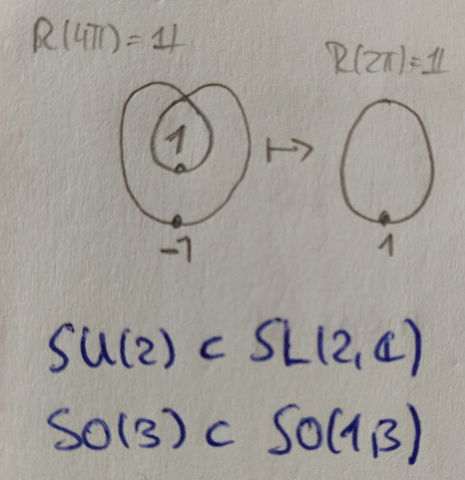
\includegraphics[width=0.7\linewidth]{gfx/doublecoverDiracSpinor}
	\caption{\itshape Double cover of the group, need to rotate by $4\pi$ to get back to the origin.}
	\label{fig:doublecoverdiracspinor}
\end{figure}

$\Rightarrow \psi_L, \psi_R$ transform under the irreducible representation of SO(1,3), $\psi=(\psi_L, \psi_R)^T$ only transforms under the reducible representation of Spin(1,3).

\subsection{Lorentz tensor- and spinor-fields}
Fields $\psi(x)$ transforming under Lorentz transformations of the coordinates $x^\mu \rightarrow x^{\prime \mu} = \Lambda^\mu_\nu x^\nu$ as
\begin{equation}
\label{eq:fieldsLorentztrafo}
	\psi(x) \rightarrow \psi^\prime(x^\prime) = D(\Lambda) \psi(\Lambda^{-1}x^\prime)
\end{equation}
with the \todo{Work through gregors script on Lorentz group}
Spinor representations of $L^\uparrow_+$ are ordinary representations of $SL(2, \mathbb{C})$, which is the double cover of $L^\uparrow_+ ≡ SO(3, 1)$.







\chapter{Quantum Field Theory, canonical quantization}
\begin{mybox}{Summary of QFT idea}
	In quantum field theory of point particles, the force between two particles is mediated by the exchange of virtual (or off-shell) particles. Associated with each force is a charge. Charged particles feel the force by coupling to or interacting with the particles that carry the force. The most familiar example is electrodynamics. The particles that feel the force carry electric charge. The electromagnetic force is mediated by the exchange of spin-1 photons. The photons themselves are uncharged and therefore do not directly couple to each other. The resulting field equations are linear. In QCD, a theory of the strong force built from a Yang-Mills gauge theory (the strong force is responsible for holding together nucleons and thereby the nucleus), the charge is called colour. The fundamental particles that feel the strong force are coloured quarks, and the particles that carry the force are called gluons. The gluons themselves are colour charged, hence, unlike the photon, they can directly interact with each other, and the resulting field equations are nonlinear. 
\end{mybox}
\begin{mybox}{Geometrical Interpretation of gauge QFTs}
	Presently we have a geometrical interpretation of classical gauge theories such as electrodynamics and Yang-Mills. The vector potential $A^a_{\mu}$ are connection coefficients on a principal fiber bundle where the structure group is the gauge group ($U(1)$ for electromagnetism, $SU(2)$ for Yang-Mills, and $SU(3)$ for classical chromodynamics). The field strengths $F_{\mu \nu}$ (i.e., the electric and magnetic fields in electrodynamics) are the curvatures associated with the connections (the potentials). The charged matter that the fields couple to are associated vector bundles. From this path integral viewpoint, Quantum Electrodynamics and Quantum Chromodynamics amount to integrals over the space of connection on principal fiber bundles. 
	Compare \ref{subsec:GaugeTheoriesInterpretation}.
\end{mybox}

\section{Renormalization}
In the process of renormalization, counterterms are generated to cancel the high energy or ultraviolet divergences that are encountered in the individual terms of the perturbation series. When the renormalization process is successful, the counterterms build a finite effective action that can be thought of as classical field theory that contains all of the quantum effects. The possible counterterms are consistent with the symmetries of the original bare action. In other words, internal symmetries can severely restrict the types of counterterms that can be generated and thereby limit the number of corresponding divergences. Hence, theories with more symmetry are generally more convergent.
\section{Regularization}


\section{On the transition to a quantized field theory}
The idea now is to take the equations of classical field theory and develop a quantization scheme analogously to quantizing classical point theory. Recall that in point theory we had the fundamental Poisson-brackets
\begin{equation}
	\{q_i,q_k\}_P==, \quad \{p_i,p_k\}_P=0,\quad \{q_i,p_k\}_P=\delta_{ik}
\end{equation}
which we modified to quantize the dynamical variable of point theory $x$ and $p$ by demanding
\begin{equation}
	[\hat{ x}_i,\hat{ x}_j]=0,\quad [\hat{p}_i,\hat{p}_j]=0\quad [\hat{ x}_i,\hat{p}_j]=i\delta_{ij}.
\end{equation}
You will see how closely we will continue this idea in the context of the dynamical variables of field theory $\phi$ and the conjugate field $\pi$.\\
\\
Following quantization, we will have to very carefully rethink results of classical field theory (FT), since we are now dealing with completely altered objects. ONe of the central identities from FT that is no loner true in QFT is the Hamiltonian principle
\begin{equation}
	\delta S=0.
\end{equation}
Even though we will carry the free equations of motion over to QFT, after solving the interacting equations as operator equations we will encounter so called off-shell fields, i.e. fields that do not follow the path of extreme action and therefore do not obey the classical equations of motion. In Feynman's approach of pathintegrals we will eventually be able to replace Hamilton's principle by a much more powerful one which keeps Hamilton's principle as the limit of the most likely (but not exclusive) path.\\
\\
Another statement that does not necessarily hold for quantized systems is Noether's theorem: \\
the symmetry of a Lagrangian can be broken by quantization which we will see much later in the context of \emph{anomalous symmetries}. An example will be the axial symmetry of the Dirac field. All of this is most elegantly discussed in Feynman's pathintegral formulation later on.
\subsection{Principles of quantum theory}
\begin{mybox}{}
The following postulates of QM are taken over to QFT:
\begin{enumerate}
	\item States are normalized elements of a Hilbert space
	\begin{equation}
	\label{eq:statenormalization}
		\ket{\psi_n} \in \mH \; \mathrm{with} \; \abs{\braket{\psi_n}{\psi_n}}^2 =1 \;\mathrm{for\;all\;} n,
	\end{equation}
	\item Observables are eigenvalues of hermitian operators on that Hilbert space
	\begin{equation}
		\mathcal{O}=\mathcal{O}^\dagger,
	\end{equation}
	\item Transition probabilities between states are squares of scalar products on that Hilbert space
	\begin{equation}
	\label{eq:transitionprob}
		P(\psi \rightarrow\psi_n) = \abs{\braket{\psi}{\psi_n}}^2.
	\end{equation}
	
\end{enumerate}
\end{mybox}
The normalization \ref{eq:statenormalization} makes it possible to interpret \ref{eq:transitionprob} as probabilities since only then is
\begin{equation}
	\sum_n \abs{\braket{\psi}{\psi_n}}^2 =1
\end{equation}
and the hermiticity of the operators associated with observables makes it possible to interpret its eigenvalues as results of measurements, since only then are the eigenvalues real, i.e.
\begin{equation}
	\mathcal{O}\ket{\psi_\lambda} = \lambda \ket{\psi_\lambda} \; \mathbb{with}\; \lambda \in \mR \mathrm{\;for\;all\;} \psi_\lambda.
\end{equation}
Since these axioms carry over to QFT, QM is not useless at all. In fact all the structures found in QM will carry over to QFT and simply be supplemented by the principle of relativity. It is this combination of axioms that will inevitably lead to QFT. QFT will explain the appearance of the half integer spin, where the Landé factor between the magnetic moment $\mu$ and the momentum $J$ was needed initially
\begin{equation}
	\mu^i = - g \mu_B J^i
\end{equation}
to match experiment with an input parameter not predicted by QM. In QFT, we will understand it as an implication of Lorentz invariance and even derive the Landé factor from these first principles. The ad hoc definition of momentum operators 
\begin{equation}
	[J^\alpha,J^\beta]=i\epsilon^{\alpha \beta}_\gamma J^\gamma
\end{equation}
can be understood as part of a defining commutator of the Lorentz group.\\
\\
Furthermore, we will be able to understand the appearance of gauge invariance in the classical field theory of electrodynamics
\begin{equation}
	\phi \rightarrow\phi + \frac{\partial \chi}{\partial t} \quad \& \quad \vec{A}\rightarrow \vec{A}+\vec{\nabla}\chi
\end{equation}
as a necessity of implementing Lorentz invariance in the Hilbert space of massless spin $1$ particles.\\
\\
In fact all of QM will be contained in QFT as the limit of zero spatial dimension $d\rightarrow0$, i.e. QM should be quantum quantum point mechanics as CM should be called classical point mechanics since it is the limit $d\rightarrow0$ of classical field theory. All of classical field theory will furthermore be contained in QT as the limit $\hbar \rightarrow0$, which will be most obvious in the pathintegral formalism of QFT. The limit $c\rightarrow\infty$ brings us from relativistic field theory to non-relativistic field theory, and from there $d\rightarrow0$ finally brings us to classical point mechanics just as $\hbar \rightarrow 0$ brings us there from QM. Everything prior to QFT is therefore just an approximation of QFT in certain limits.\\
\\
Taking over the principles of QM also entails taking over the discussions around the interpretation of quantum theories, which are still relevant today. For example whter a probabilistic axiom such as \ref{eq:transitionprob} should exist in a fundamental theory is still discussed.\\
\\
QM is often called non-deterministic in this context, but this is misleading. QM is probabilistic \emph{and} deterministic in its prediction of these probabilities. The evolution of the states is completely determined by the eom, which we will soon find. It is only non-deterministic in its prediction of a \emph{single} measurement, but does determine exactly the evolution of probability distributions and thereby the result that \emph{infinitely many } measurements will converge to. Of course, this kind of talk about infinitely many measurements is exactly the source of doubt over the usefulness of a probabilistic axiom and the question stans why probabilities should ever come into play if there are deterministic equations working in the background. Maybe more obviously problematic is the introduction of observables via hermitian operators, which makes a fundamental distinction between an "observer" and the system which is described by the observer by mentioning an "observable". Surely if the theory is fundamental it should \emph{describe} the observer and the measurement process and not simply postulate the collapse of a state. The distinction between a measurement apparatus and the measured object should arise from the theory and not be hard-wired into it at the axiomatic level. It seems that mentioning an observer is really the same as mentioning consciousness and doing so in an axiomatic way means giving up on ever explaining how consciousness arises from first principles.


\subsection{Wigner's theorem}
If a system of states $\{\psi,\psi_1,\dots\}$ has a symmetry $U$ such that
\begin{equation}
	\abs{\braket{\psi}{\psi_n}}^2 = \abs{\braket{\psi^\prime}{\prime^\prime_n}}^2 \mathrm{\, for\,all\,n\, as\, \psi \rightarrow \psi^\prime}
\end{equation}
i.e. the postulated probability of transition is invariant, then
\begin{align}
	\braket{U\psi}{U\psi_n} &= \braket{\psi}{\psi_n} \; \mathrm{and} \; U(\alpha \psi + \beta \psi_n) = \alpha U \psi + \beta U \psi_n \\
	or \braket{U\psi}{U\psi_n} &= \braket{\psi}{\psi}^* \; \mathrm{and\;} U(\alpha \psi+ \beta \psi_n) = \alpha^* U\psi + \beta^* U \psi_n
\end{align}
i.e. $U$ is either linear and unitary or antilinear and antiunitary.
\subsection{Lorentz invariance in quantum theory}
Transformation of a state via $\infty$-dimensional unitary representation $U(\Lambda)$ (acc. to Wigner)
\begin{equation}
	\ket{\alpha}\rightarrow \ket{\alpha^\prime} = U(\Lambda) \ket{\alpha} \;\mathrm{with}\; UU^\dagger = \mathcal{I}.
\end{equation}
Alternatively we can interpret this as a transformation of the field operator where $x\rightarrow\Lambda x$ as
\begin{equation}
	\psi(x) \rightarrow \psi^\prime(x^\prime) = U^{-1}(\Lambda)\psi(\Lambda^{-1} x^\prime) U(\Lambda) \stackrel{\ref{eq:fieldsLorentztrafo}}{=} D(\Lambda) \psi(\Lambda^{-1}x^\prime).
\end{equation}
Analogously to $\phi^\prime(x^\prime) = \phi(x)$ in classical field theory, we now define a quantized scalar field as
\begin{equation}
	\bra{\alpha^\prime}\phi(x^\prime) \ket{\beta^\prime} = \bra{\alpha} \phi(x) \ket{\beta} \; \Leftrightarrow\; \phi(x) \mathrm{\,is\,a\,scalar\,field}
\end{equation}
or generally analogous to  \ref{eq:fieldsLorentztrafo}
\begin{equation}
	\bra{\alpha^\prime}\psi(x^\prime)\ket{\beta^\prime} = \bra{\alpha}D(\Lambda) \psi(\Lambda^{-1} x^\prime)\ket{\beta}.
\end{equation}
\todo{Go through different kinds of discrete and continuous symmetries in QFT}
\section{Symmetries}
\marginpar{The particle picture in QFT is useful as it is easy, but it requires a high degree of symmetry of the vacuum.}
\begin{mybox}{Definition}
A transformation $\psi(x) \rightarrow \psi^\prime (x^\prime)$ is a symmetry if it leaves the action invariant
\begin{equation}
	S[\phi] \rightarrow S^\prime [\phi^\prime] = S[\phi].
\end{equation}
\end{mybox}
\begin{mybox}{State of the symmetry in a theory}
	A symmetry is
	\begin{enumerate}
		\item unbroken \\$\Leftrightarrow$ $S\rightarrow S$ action is invariant and the vacuum is invariant $\ket{vac}\rightarrow\ket{vac}$.\\
		Most of the symmetries we know are not exact, i.e. most global symmetries are broken a little bit (little ito. scale of the system).
		\item Explicitly broken \\$\Leftrightarrow S\rightarrow S+\underbrace{\Delta S}_{\neq 0}$.
		\item Spontaneously broken\\
		$\Leftrightarrow S\rightarrow S$ is invariant, but the vacuum is not $\ket{vac}\rightarrow \ket{vac}^\prime \neq  \ket{vac}$. Thus, the particle states change here. See further \ref{sec:spontaneoussymmetrybraking}.
	\end{enumerate}
\end{mybox}
A symmetry is either
\begin{enumerate}
	\item Continuous \\
	$\Leftrightarrow$ symmetry transformations continuously depend on some parameter
	\item Discrete
\end{enumerate}
\subsection{Discrete Symmetries}
Discrete symmetries are often called $\mathbb{Z}_m$ as you rotate a point by $\frac{2 \pi}{N}$, i.e. $\mathbb{Z}_2$ rotates field $\rightarrow-$field.
\subsubsection{Parity}
$\vec{p}\rightarrow - \vec{p}$\\
Parity inversion of a scalar field operator is
\begin{equation}
	P^{-1} \phi(t,\vec{x}) P = \phi(t,-\vec{x}).
\end{equation}
The parity inversion of a vector field operator is
\begin{equation}
	P^{-1}A^\mu(t,\vec{x})P = P^\mu_\nu A^\nu(t,-\vec{x})
\end{equation}
with
\begin{equation}
P^\mu_\nu = 
\begin{pmatrix}
+1&&&\\&-1&&\\
&&-1&\\
&&&-1
\end{pmatrix}.
\end{equation}
The parity inversion of a spinor field operator with $\Lambda^{-1} \gamma^\mu \Lambda = \Lambda^\mu_\nu \gamma^\nu$ is
\begin{align}
	P^{-1}\psi(t,\vec{x})P &= P^A_B \psi^B(t,-\vec{x})\quad \mathrm{with}\\
	P^A_B&=(\gamma^0)^A_{\;B}.
\end{align}

\subsubsection{Time reversal}
$t\rightarrow-t$\\
Time inversion of a scalar field operator is
\begin{equation}
	T^{-1} \phi(t,\vec{x}) T = \phi(-t,\vec{x}).
\end{equation}
The time inversion of a vector field operator is
\begin{equation}
	T^{-1} A^\mu(t,\vec{x})T = T^\mu_\nu A^\nu(t,-\vec{x})
\end{equation}
with
\begin{equation}
T^\mu_\nu=
\begin{pmatrix}
-1&&&\\&+1&&\\
&&+1&\\
&&&+1-
\end{pmatrix}.
\end{equation}
The time inversion of a spinor field operator with $\Lambda^{-1} \gamma^\mu \Lambda = \Lambda^\mu_\nu \gamma^\nu$ is
\begin{align}
	T^{-1}\psi(t,\vec{x}) T &= T^A_B \psi^B(-t,\vec{x})\quad \mathrm{with}\\
	T^A_{\;B} &=-i(\gamma^1\gamma^3)^A_{\;B}.
\end{align}
The infinite dimensional representation of $T$ is anti-unitary and anti-linear.
\subsubsection{Charge conjugation}
 $e^- \rightarrow e^+$\\
 Charge conjugation is given by
 \begin{align}
 	C^{-1}\psi(x)C &= -i (\bar{\psi}(x) \gamma^0 \gamma^2)^T\\
 	C^{-1} j^\mu(x) C &= - j^\mu(x)\\
 	C^{-1} A^\mu(x) C &= - A^\mu(x).
 \end{align}
 \subsubsection{Discrete symmetries (CPT)}
Whether a theory is parity, time inversion or charge conjugation invariant, i.e. whether $P\ket{\Omega}=\ket{\Omega}$,$T\ket{\Omega}=\ket{\Omega}$, $C\ket{\Omega}=\ket{\Omega}$ has to be tested case by case, e.g. weak interactions are \emph{not} charge conjugation invariant (but invariant under the combination $CPT$); the electromagnetic interactions are invariant under $P,C,T$ individually.
\subsubsection{CPT-theorem}
\begin{mybox}{CPT-theorem }
	For a Lorentz invariant theory with a stable vacuum, i.e. a vacuum with an energy expectation value that is bounded from below,
	one has
	\begin{equation}
	\label{eq:cpttheorem}
		CPT \ket{\Omega}=\ket{\Omega}.
	\end{equation}
\end{mybox}. 
in any reasonable QFT we therefore have $CPT=\mI$. CP is not conserved in the SM (CKM matrix rotates quarks and leading to mixing).
\subsubsection{Dark Matter}
Dark matter has to be cosmologically stable (i.e. lives longer than the age of the Universe), how can you protect DM from decay ?\\
One possibility are Beyond SM theories (BSM) 
\begin{equation*}
	BSM = [SM] \otimes [DS],
\end{equation*}
where the dark sector $[DS]$ has to contain DM as its lightest particle which has to be stable. Hypothesize there to exist a $\mathbb{Z}_2$ symmetry:
\begin{equation*}
	fields_{SM} \stackrel{\mathbb{Z}_2}{\rightarrow} fields_{SM}
\end{equation*}
are invariant, but 
\begin{equation*}
	fields_{DS} \stackrel{\mathbb{Z_2}}{\rightarrow} - fields_{DS}.
\end{equation*}
Where the symmetry is constrained by the general requirement that \emph{DM has to interact with SM in some way, because otherwise it would not have been produced at Big Bang in the first place}.\\
This symmetry is the simplest possibility to make DM stable (prohibits decay into SM, can only be produced in pairs due to $\mathbb{Z}_2$ symmetry of initial and final state). Thus logic is to postulate a discrete symmetry under which DM has parity $-1$, whilst SM is invariant under it.\\
\todo{Look into this} We know that there has to be a mixing of the SM and dark sector, i.e. there being possible interactions beside gravity, as otherwise DM would not have been produced after BB in the first place (decoupled then).
\subsubsection{Field symmetry}
Could have $\mathbb{Z}_2$ symmetry of real scalar field $\phi^4$ theory which is symmetry under $\phi \rightarrow - \phi$.
\subsection{Continuous symmetry}
Consider for example a complex scalar field theory, which would be invariant under $U(1)$ symmetry $\phi(x) \rightarrow e^{-i \alpha} \phi(x)$, a continuous symmetry as $\alpha$ is a continuous parameter.
\begin{mybox}{Types of continuous symmetry}
We distinguish continuous symmetries between
\begin{enumerate}
	\item global, i.e. for $\alpha=$constant.
	\item local, i.e. for $\alpha=\alpha(x)$ a function depending locally on spacetime. Note that for $U \in$ $G_{\text{symmetry group}}$, where $G$ is a Lie group as we are considering a continuous symmetry, if
	\begin{equation*}
		U = U(x) \Leftrightarrow \text{local symmetry } \Leftrightarrow \text{ gauge symmetry}.
	\end{equation*}
	\item Note that the process of promoting $\alpha \rightarrow \alpha(x)$ a global to a local symmetry is called \emph{gauging}, c.f. QED.
\end{enumerate}
\end{mybox}
\begin{mybox}{Noether current }
	Every global, continuous symmetry has a conserved Noether current associated with it, which then again has a time independent Noether charge
	\begin{equation*}
	Q=\int \md^3 x j(x),\quad \frac{\md Q}{\md t}=0,
	\end{equation*}
i.e. the charge is a conserved quantity. Note further that it holds that
\begin{statements}
$\#$ generators of symmetry $=\#$ Noether currents $=\#$ conserved charges. 
\end{statements}
See further \ref{subssec:noethersymmetries}.
\end{mybox}
\subsection{Gauge symmetries}
Gauge symmetries are continuous local symmetries.\\
Note that global and gauge symmetries are on a very different footing:
\begin{enumerate}
	\item A gauge symmetry is a redundancy of the description of the system.
	\item A global symmetry is a true symmetry between different field configurations.
\end{enumerate}
\subsubsection{How do we construct abelian gauge theories -- Doppelt sich mit QED part von Weigand --  crude description}
 For example consider $\mL_D$ where the Dirac fermion is invariant under a global $U(1)$ transformation $\psi(x)  \rightarrow e^{-i e \alpha} \psi(x)$, the Noether charge is the electric charge $e=Q \abs{e}, Q_D=\pm 1$ of $\psi,\bar{ \psi}$.\\
Now we make the transformation local, it will not be invariant under $U(1)$ anymore
\begin{equation*}
	U(x) = e^{-i e\alpha(x)} \Rightarrow \mL \rightarrow\mL+ \underbrace{\bar{ \psi}i \gamma^\mu \psi (-i \partial_\mu \alpha(x))}_{\neq 0}.
\end{equation*}
Modify the Lagrangian therefore in order to make it invariant under the local continuous symmetry, i.e. to make it gauge invariant. For this endeavour , we add compensating fields, nowadays known as \emph{gauge fields}. The fields transform like
\begin{equation}
	\psi(x) \rightarrow U(x) \psi(x), \quad \bar{ \psi}(x) \rightarrow\bar{ \psi}(x) U^\dagger(x)
\end{equation}
and we add a gauge field $A_\mu(x)$ which we require to transform like the following under the gauge transformation
\begin{equation}
	A_\mu(x)\rightarrow U(x) \left[A_\mu(x) - \frac{i}{e} \partial_\mu\right] U^\dagger(x) = A_\mu(x) + \frac{1}{e} \partial \alpha(x).
\end{equation}
Then we can make $\mL$ gauge-invariant by introducing the $U(1)$ \emph{gauge covariant derivative} $D_\mu = \partial_\mu + i e A_\mu$, such that
\begin{equation}
	\mL_D \stackrel{\partial_\mu \rightarrow D_\mu}{\longrightarrow} \mL_{QED}=\bar{ \psi}(i \slashed{D}-m) \psi - \frac{1}{4}F\munu F^{\mu\nu}.
\end{equation}
The resulting Lagrangian has the following properties
\begin{enumerate}
	\item It is gauge invariant by virtue of coupling the fermion to the gauge field $A_\mu$ via the gauge coupling constant of our gauge theory $U(1)$, the gauge invariance of the Lagrangian is due to the transformation behaviour of the gauge field by construction.
	\item Gauge symmetry of the Lagrangian then implies interactions ($3$vertex $\psi \slashed{A}\bar{ \psi}$) due to the coupling to the gauge field
	\item The gauge field has a propagating degree of freedom, i.e. the kinetic term $\tr(F^2)$.
	\item Note that objects like $( \partial_\mu A_\nu)(\partial^\mu A^\nu)$ and $m^2 \half A_\mu A^\mu$ are not gauge invariant.
\end{enumerate}
\begin{mybox}{Minimal coupling scheme}
	In total we made the Lagrangian gauge-invariant by two steps
	\begin{equation}
		\partial_\mu \rightarrow D_\mu,\quad \oplus \frac{1}{4} F\munu F^{\mu \nu}
	\end{equation}
	which is the so-called \emph{minimal coupling scheme} as it automatically includes interactions by construction. Note that the vertex of this interaction, i.e. $-e \gamma^\mu$ in QED, is fixed by gauge invariance.
\end{mybox}
\subsubsection{How do we construct a non-abelian gauge theory - Crude description}
This is a broad description, for more details see further down in \ref{sec:nonabeliangaugetheory}. \\
A non-abelian gauge theory is called a Yang-Mills theory, with a non-abelian gauge group $SU(N)$ and transformations $U(x) = e^{-i T^a \theta^a}$, where $T^a,a=1,\dots,N^2-1$ are the generators of the gauge group.\\
Again we can construct a gauge-invariant Lagrangian via the minimal coupling scheme, but the order of operators in the transformation matters now. We have for $\mL_D$
\begin{equation}
	\psi(x) \rightarrow U(x) \psi(x),\quad \bar{ \psi}(x) \rightarrow \bar{ \psi}(x) U^\dagger(x)
\end{equation}
and we again add a gauge field which we require to transform like
\begin{equation}
	A_\mu(x) \rightarrow U(x) \left[ A_\mu + i \partial_\mu\right]U^\dagger(x),
\end{equation}
note the different trafo behaviour to the abelian case. Introduce the non-abelian gauge covariant derivative $D_\mu = A_\mu - i \partial_\mu$, the field strength is now
\begin{equation*}
	F\munu = \partial_\mu A_\nu-\partial_\nu A_\mu - i [A_\mu,A_\nu].
\end{equation*}
We repackage the gauge fields and field strengths via matrix notation
\begin{equation*}
	A_\mu = g T^a A^a_\mu, \qquad F\munu= g T^a F^a\munu,
\end{equation*}
with $g$ the coupling constant of the gauge group. Then we find this particular Yang-Mills Lagrangian to be
\begin{equation}
	\mL = \bar{ \psi} (i\gamma_\mu D^\mu -m) \psi - \frac{1}{2 g^2} \tr (F\munu F^{\mu \nu}).
\end{equation}
This is just a motivation, look further in \ref{sec:nonabeliangaugetheory}.






































\section{The Free Scalar Field}
\subsection{Why Quantum Field Theory?}
QFT describes a many-body system through fields as fundamental entities. These are abstract object that penetrate spacetime by describing the distribution of some physical quantity. Then particles are the excitation of the field, the quantums of oscillation of an abstract field.\\
QM is then QFT's non-relativistic limit, it's a quantum field theory in zero spatial dimensions ($\equiv$ time dimension),
because the combination of QM and SR implies that \emph{particle number is not conserved}, because all particles of the same type are \emph{the same}. Particles are the excitations of one particular specific field that penetrates spacetime, therefore their nature doesn't depend on time and space of their creation.\\
Universality and renormalization are central concepts of QFT, i.e. different "microscopic" theories can describe the same "macroscopic" observable physics.
\subsubsection{Natural Units}
We use natural units, where 
\begin{align*}
	\hbar &= c = 1 \; \Rightarrow \; [energy]=[mass]=[length]^{-1}=[time]^{-1} \\
	\Rightarrow \alpha &= \frac{e^2}{\hbar c}.
\end{align*}
If $X$ has dimensions $(mass)^d$ we will write $[X]=d$.


\subsection{Schrödinger equation and the Schrödinger picture}
\begin{mybox}{Schrödinger equation}
	\begin{equation}
		i \partial^0 \ket{\psi} = H^0 \ket{\psi}.
	\end{equation}
\end{mybox}
The Schrödinger picture has the advantage that it makes manifest the linear nature of QFT, which is the same as that of QM. Another natural property of this formulation is that the "wavefunction" formalism of old fashioned QM can be obtained as the limit of zero spatial dimensions from the "wavefunctional" formalism, which is obtained from the Schrödinger equation.
\subsection{Heisenberg equation and Heisenberg picture}
\begin{mybox}{Heisenberg equation}
	\begin{equation}
	\frac{\md \mathcal{O}}{\md t} = i [H,\mathcal{O}].
	\end{equation}
\end{mybox}
The Heisenberg picture has the advantage that field operator equations of motion can directly be derived from a manifestly Lorentz invariant variational principle of a quantum action which for free theory coincides with classical field theory. Just like in the Lagrangian picture of classical field theory, properties of symmetry and locality are manifest in this picture.
\subsection{Causality}
\begin{mybox}{}
	\begin{equation}
			[\mO_i(x),\mO_j(y)] = 0 \; \mathrm{for}\; (x-y)^2 <0 \mathrm{\; and \, all \,operators}.
	\end{equation}
\end{mybox}
Note that this statement holds true for arbitrary $x^0,y^0$ while the quantizing commutations relations are all equal time relations.
\subsection{Uncertainty}
\begin{mybox}{}
	\begin{align}
		\langle (\Delta \mO_1)^2\rangle \langle (\Delta \mO_2)^2 \rangle &\geq \frac{1}{4} \abs{\langle [\mO_1,\mO_2]\rangle}^2\\
		 \mathrm{\,for\,all\,states,\,and\,} \Delta \mO_i&:= \mO_i -\expval{\mO_i}.\nonumber
	\end{align}
\end{mybox}


\subsection{Classical Scalar Field, Lagrangian Formulation}













By starting with a classical action for a finite number of d.o.f. $q_i(t)$ 
\begin{equation}
	S[q_i] = \int_{t_1}^{t_2} \md t \; L(q_i(t),\dot{q}_i(t)),
\end{equation}
we can make the transition to a scalar field $\phi(t,\vec{x})=\phi(x^{\mu})$ by replacing:
\begin{enumerate}
	\item[First step:] 
	\begin{equation}
		q_i \rightarrow \phi(x^{\mu}),\quad \dot{q}_i \rightarrow \frac{\partial \phi(x^{\mu})}{\partial t},
	\end{equation}
	where we consider a \emph{real} scalar field $\phi:x^{\mu} \rightarrow \phi(x^{\mu}) \in \mR$ that describes \emph{spin-zero} particles 
	\begin{equation}
		S = \int \md^4 x \; \mathcal{L}(\phi(x),\partial_{\mu} \phi(x)),
	\end{equation}
	with $[\mathcal{L}]=4,[S]=0, [\md^4 x]=-4$. This system has an infinite number of degrees of freedom (at least for each point $\vec{x}$ in space).
	\item[Second Step:] Find the Lagrangian:\\
	$\mathcal{L}$ is a Lorentz-scalar and therefore has to depend only on Lorentz-scalars in a relativistic setting.
	\begin{equation}
		S = \int \md^4 x \left[\frac{1}{2} \underbrace{\partial_{\mu}\phi \partial^{\mu} \phi}_{=(\partial \phi)^2} -V(\phi) + \mathcal{O}(\phi^n (\partial \phi)^m)\right],
	\end{equation}
	where $m\geq2 \& n\geq1$ can be left out doesn't change physics.
	Note that the Lagrangian is \emph{local}. No terms in $\mathcal{L}$ that couple $\phi(\vec{x})$ to $\phi(\vec{y}): \Leftrightarrow \mathcal{L}=\mathcal{L}\left(\phi(\vec{x},t),\dot{\phi}(\vec{x},t), \vec{\nabla} \phi(\vec{x},t)\right)$. Only consider $\mathcal{L}$ depending on $\nabla\phi$ and not on higher derivatives, because they are not Lorentz-invariant.\\
	$\partial_{\mu}\partial^{\mu}\phi$ is a \emph{total derivative} and therefore does not alter e.o.m. due to assumptions of boundary terms which can be left out.\\
	Note that
	\begin{align}
		[\phi] &= \mathrm{mass}^1 = \frac{d}{2} -1 \\
		 \Rightarrow \mathcal{L} (\mathrm{scalar \; field, \; real}) &= \frac{1}{2} \eta^{\mu \nu} \partial_{\mu} \phi \partial_{\nu} \partial - \frac{m^2}{2} \phi^2 \nonumber \\
		 &= \frac{1}{2} \dot{\phi}^2 - \frac{1}{2} (\nabla \phi)^2 - \frac{m^2}{2} \phi^2.
	\end{align}
\end{enumerate}
By assuming a global minimum for $V(\phi(x))$ at $\phi_0(x)$ we can expand 
\begin{equation}
	V(\phi(x)) = V_0 + \frac{m^2}{2} \phi^2(x) + \mathcal{O}(\phi^3(x)),
\end{equation}
with\footnote{Note that a minus sign in front of the mass term would imply an unstable potential, i.e. a downward facing parabola. This would describe a Tachyon.} $V_0$ the classical contribution to the ground state or vacuum energy. Higher power of $\phi^{>2}$ in the potential $V(\phi)$ as well as the terms $\mathcal{O}(\phi^n(\partial \phi)^m)$ will give rise to interactions between the particles. Taking these terms into account gives rise to interaction and therefore the field would be described by infinitely anharmonic coupled oscillators:
\begin{mybox}{Free scalar field theory}
	\begin{equation}
		S = \int_{\mR^{3,1}} \md^4x \; \left[\frac{1}{2} (\partial \phi)^2 - \frac{m^2 \phi^2}{2}\right],\quad \phi=\phi^*.
	\end{equation}
\end{mybox}


\begin{mybox}{Klein-Gordon equation}
	I.e. for the free scalar field this yields the
	\begin{equation}	
	(\partial^2+m^2) \phi(x)=0,
	\end{equation}
\end{mybox}


\subsection{Canonical Quantization in the Schrödinger Picture}
Begin with the replacement $q_i \rightarrow \phi(\vec{x},t)$ and the conjugate momentum 
\marginpar{The fields vanish at spatial boundaries. They also vanish inside action evaluated at time boundaries, because action has fixed timepoints.}
\begin{equation}
	p_i = \frac{\partial \mathcal{L}}{\partial \dot{q}_i} \quad \rightarrow \quad \Pi(\vec{x},t):= \frac{\partial \mathcal{L}}{\partial \dot{\phi}(\vec{x},t)}
\end{equation}
with $\Pi$ the \emph{conjugate momentum density}.\\
The Hamiltonian is
\begin{equation}
	H=\int \md^3x\mathcal{H} =\int \md^3 x \left[\Pi(\vec{x},t) \dot{\phi}(\vec{x},t) - \mathcal{L}\right],
\end{equation}
which for the free scalar field is
\begin{equation}
	H = \int_{\mR^3} \md^3 x \left[\frac{1}{2} \dot{\phi}^2 + \frac{1}{2} (\vec{\nabla} \phi)^2+ \frac{m^2}{2} \phi^2 \right].
\end{equation}

To quantize in the Schrödinger picture we go over to
\begin{equation}
	\phi^{(s)} (\vec{x}) = \left(\phi^{(s)}(\vec{x}\right)^{\dagger}, \qquad \Pi^{(s)}(\vec{x})=\left(\Pi^{(s)} (\vec{x})\right)^{\dagger}
\end{equation}
self-adjoint and time independent (all time dependence lies in the states) scalar field operators with the \emph{canonical commutation relations}
\begin{align}
	\left[\phi(\vec{x}),\Pi(\vec{y}) \right] &= i \hbar \delta^{(3)}_D (\vec{x}-\vec{y})= i \delta^{(3)}_D (\vec{x}-\vec{y}),\\
	 \left[\phi(\vec{x}), \phi(\vec{y})\right]&=0, \; \left[\Pi(\vec{x}), \Pi(\vec{y})\right]=0.
\end{align}
Note that this is analogous to the canonical commutation relations of QM, where we quantized $x$ and $p$. This is no longer demanded in QFT. There is no second quantization as historically misunderstood. The only quantized objects from CFT are the fields. Momentum and psace are those of CFT, where they are mere labels of the fields.\\
Also note that although this method of quantization is not manifestly Lorentz invariant (since $\pi(x)$ transforms like the $0$-component of a $4$-vector), it will nevertheless lead to a Lorentz invariant formulation of observables, as will become apparent in the following. For a manifestly Lorentz invariant formulation compare pathintegral quantization.
\subsection{Mode Expansion}
For the example of the free scalar field theory:\\
The classical Lagrangian describes an infinity of coupled harmonic oscillators. Because the coupling is described by $\vec{\nabla}$ with eigenfunctions $e^{i \vec{p} \vec{x}}$, interaction will be diagonal through a Fourier transform
\begin{align}
	\phi(\vec{x}) &= \int \frac{\md^3 p}{(2\pi)^3} \tilde{\phi}(\vec{p}) e^{i \vec{p} \vec{x}} \\
	\Pi (\vec{x}) &= \int \frac{\md^3 p}{(2 \pi)^3} \tilde{\Pi}(\vec{p}) e^{i \vec{p}\vec{x},}
\end{align}
with the reality of the fields ensuring $\tilde{\phi}^{\dagger}(\vec{p})=\tilde{\phi}(-\vec{p}), \tilde{\Pi}^{\dagger}(\vec{p})=\tilde{\Pi}(-\vec{p})$.
One uses the identity of the Dirac distribution 
\begin{equation}
	\int \md^3 x e^{i(\vec{p}+\vec{q}) \vec{x}} = (2 \pi)^3 \delta^{(3)}_D(\vec{p}+\vec{q}).
\end{equation}
This implies the form of the quantized Hamiltonian
\begin{equation}
H = \frac{1}{2} \int \frac{\md^3 p}{(2\pi)^3} \left[\underbrace{\tilde{\Pi}(\vec{p}) \tilde{\Pi}^{\dagger}(\vec{p})}_{=|\tilde{\Pi}(\vec{p}) |^2} + \omega^2_p \underbrace{\tilde{\phi}(\vec{p}) \tilde{\phi}^{\dagger}}_{=|\tilde{\phi}(\vec{p})|^2}\right],
\end{equation}
with $\omega^2_p = \vec{p}^2+m^2$. This is a collection of \emph{decoupled harmonic oscillators} with frequency $\omega_p$ with momentum $p$.\\
The collective Hilbert space of all these oscillators is thus constructed using \emph{creation} and \emph{annihilation} operators constructed from these modes. We define the operators:
\begin{align}
	\hat{a}(\vec{p})&= \frac{1}{2} \left[\sqrt{2 \omega_p} \tilde{\phi}(\vec{p}) + o \sqrt{\frac{2}{\omega_p}} \tilde{\Pi} (\vec{p})\right]; \\
	 \tilde{\phi}(\vec{p}) &= \frac{1}{\sqrt{2 \omega_p}} \left[\hat{a}(\vec{p}) + \hat{a}^{\dagger}(-\vec{p})\right] \\
	\hat{a}^{\dagger}(\vec{p}) &= \frac{1}{2} \left[\sqrt{2 \omega_p} \tilde{\phi}(-\vec{p}) -i \sqrt{\frac{2}{\omega_p}} \tilde{\Pi}(-\vec{p})\right],\\
	 \tilde{\Pi}(\vec{p}) &=-i \sqrt{\frac{\omega_p}{2}} \left[\hat{a}(\vec{p}) - \hat{a}^{\dagger} (-\vec{p})\right],\\
	\mathrm{with} \; \left[\tilde{\phi}(\vec{p}), \tilde{\Pi}(\vec{q}) \right] &= (2 \pi)^3 i \delta^{(3)}_D(\vec{p}+\vec{q}).
\end{align}
\begin{mybox}{Quantized space and momentum operator}
	\begin{align}
		\phi(\vec{x})&= \int_{\mR^3} \pmeasure \; \frac{1}{\sqrt{2 \omega_p}} \left[\hat{a}(\vec{p}) e^{i \vec{x}\vec{p}} +\hat{a}^{\dagger}(\vec{p})e^{ i \vec{x}\vec{p}}  \right]\\
		\Pi(\vec{x}) &= \int_{\mR^3} \pmeasure \; (-i) \sqrt{\frac{\omega_p}{2}} \left[\hat{a}(\vec{p}) e^{i \vec{p}\vec{x}} - \hat{a}^{\dagger}(\vec{p}) e^{-i\vec{p}\vec{x}} \right].
	\end{align}
\end{mybox}
The ladder operators obey the commutation relation
\marginpar{Leave hats off of operators as of now, $\hat{a}\equiv a$.}
\begin{mybox}{Commutation relations}
	\begin{align}
		\left[a(\vec{p}), a^{\dagger} (\vec{q})  \right] &= (2 \pi)^3 \delta^{(3)}_D(\vec{p}-\vec{q}) \\
		\left[a^{\dagger}(\vec{p}), a^{\dagger} (\vec{q}) \right] &=0= \left[a(\vec{p}), a(\vec{q})\right], \qquad \forall \vec{p},\vec{q}.
	\end{align}
\end{mybox}
Therefore, the Hamiltonian in its final form is given by
\begin{equation}
	H = \int_{\mR^3} \pmeasure \omega_p a^{\dagger}(\vec{p}) a(\vec{p}) \; + \; \Delta_H, \quad \omega_p = E_p =\sqrt{\vec{p}^2+m^2},
\end{equation}
where $a^{\dagger}(\vec{p}) a(\vec{p}) $ may be interpreted as the number operator $N_p$ giving the number of particles in a state with momentum $p$.\\
With the \emph{divergent ground state/zero-point energy} $\frac{\hbar \omega_p}{2}$ in
\begin{equation}
\label{eq:divergentGroundstateEnergy}
	\Delta_H = \frac{1}{2} \int \md^3 p \omega_p \delta^{(3)}_D(\vec{0}).
\end{equation}
In a theory without gravity, absolute energy has no meaning, only energy differences do. This Hilbert space possesses a state of lowest energy, the vacuum $\ket{0}$. The vacuum corresponds to the absence of any excitations of the field $\phi$.\\
\\
There is a deeper reason for constructing the Hamiltonian out of creation and annihilation operators, which has nothing to do with whether particles can actually be produced or destroyed. The great advantage of this formalism is that if we express the Hamiltonian as a sum of products of creation and annihilation operators, with suitable non-singular coefficients, then the S-matrix will automatically satisfy a crucial physical requirement, the \emph{cluster decomposition principle}, which says in effect that distant experiments yield uncorrelated results. Indeed, it is for this reason that the formalism of creation and annihilation operators is widely used in non-relativistic quantum statistical mechanics, where the number of particles is typically fixed. In relativistic quantum theories, the cluster decomposition principle plays a crucial part in making a field theory inevitable. It is one of the fundamental principles of physics that experiments that are sufficiently separated in space have unrelated results.The cluster decomposition principle together with Lorentz invariance makes it natural that the interaction density should be constructed out of the annihilation and creation fields.\\
The Hamiltonian obeys the commutation relations
\begin{align}
	\left[H,a(\vec{p})\right] &= - \omega_p a(\vec{p}) \\
	\left[H,a^{\dagger}(\vec{p})\right] &= \omega_p a^{\dagger}(\vec{p}).
\end{align}
Or rather by combining $H$ and the spatial momentum operator
\begin{equation}
	p^i = \int \pmeasure \; p^i a^{\dagger} (\vec{p}) a(\vec{p}) \quad + \underbrace{\Delta_{p_i}}_{=\frac{1}{2} \int \md^3 p \; p^i \delta^{(0)}_D(0) \equiv 0 }
\end{equation}
to the \emph{4-momentum operator}
\begin{equation}
\label{eq:fourmomOperator}
	P^{\mu} = \int_{\mR^3} \pmeasure \; p^{\mu} a^{\dagger}(\vec{p}) a(\vec{p}) \quad+ \Delta_{p^{\mu}}, \quad \Delta p^{\mu} = \left\{ \begin{array}{lr}
	\Delta H & \mu =0 \\
	0 & \mu=1,2,3.
	\end{array}\right\},
\end{equation}
with $p^{\mu} =(p^0,\vec{p})= (\omega_p, \vec{p})$.
\begin{mybox}{Momentum operator of the real scalar field}
The momentum operator is hermitian $P^\mu=(P^\mu)^\dagger$.\\There exists a common set of eigenstates of $H$ and $\vec{P}$, i.e. $\vec{P}$ is locally conserved, the system is translation invariant and
\begin{equation}
	[H,\vec{P}]=0.
\end{equation}
The momentum operator obeys
\begin{equation}
	\partial^\mu \phi = i[P^\mu,\phi]
\end{equation}
which generalizes the Heisenberg equation
\begin{equation}
	\phi(x+a) = e^{i a_\mu P^\mu} \phi(x) e^{-ia_\mu P^\mu}
\end{equation}
which then again identifies the $4$-momentum as the generator of space-time translations.
\end{mybox}
Note that as for any result obtained by using Noether's theorem, we could have obtained the energy-momentum tensor in CFT already. Only after plugging in the field operators we obtain results such as the momentum \emph{operator} \ref{eq:fourmomOperator} exclusive to QFT.\\
\\
One can look at $[H,\vec{P}]=0$ as an immediate implication of the axiom of Poincaré invariance where it is one of the defining commutators of the Poincaré algebra and \emph{prove} the quantization rules (i.e. the canonical commutation relations). Alternatively one can look at lorentz invariant Lagrangians and use the quantization rules axiomatically to \emph{prove} $[H,\vec{P}]=0$.
\begin{mybox}{Construction of the Hilbert space}
	We get the commutation relations
	\begin{align}
		\left[P^{\mu}, a^{\dagger} (\vec{p})\right] & = p^{\mu} a^{\dagger}(\vec{p}), \\
		\left[P^{\mu},a(\vec{p})\right] &= -p^{\mu} a(\vec{p}).
	\end{align}
\end{mybox}
What did we do ?\\
We have started with the assertion that spacetime (here $\mR^{1,3}$) is filled with the real scalar field $\phi(\vec{x})$, which we have taken to be a free field with Lagrangian $\mathcal{L}=\frac{1}{2} (\partial \phi)^2 - \frac{m^2}{2} \phi^2$. This field is interpreted as a field operator, i.e. in the Schrödinger picture at every space point $\vec{x}$ the object $\phi(\vec{x})$ represents a self-adjoint operator that acts on a Hilbert space. This Hilbert space possesses a state of lowest energy, the vacuum $\ket{0}$.


\subsection{The Fock space}

QM asks the question "which particle is on which state". In Qm, the particles are identical, such that exchanging two particles $(\vec{r}_i \leftrightarrow \vec{r}_j)$ does not lead to different many-body quantum states.
\begin{mybox}{spin-statistics-theorem}
	The spin-statistics theorem states, that a many-body wave function is either symmetric (bosons) or antisymmetric (fermions) under particle exchange.
\end{mybox}
In QFT one asks "how many particles are there on each state". In this approach, the many-body state is represented in the occupation number basis and the basis state is labelled by the set of occupation numbers. \\
The occupation number states $\ket{[n_{\alpha}]}$ are known as \emph{Fock states}
\begin{equation}
	\ket{[n_{\alpha}]} \equiv \ket{n_1,n_2,\dots,n_{\alpha}}
\end{equation}
meaning that there are $n_{\alpha}$ particles in the single-particle state $\ket{\alpha}$ (or as $\psi_{\alpha}$). The occupation numbers sum up to total number of particles 
\begin{equation}
	N=\sum_{\alpha} n_{\alpha}.
\end{equation}
The \emph{number operator} $N$ counts the number of particles in a given state in the Fock space
\begin{equation}
	N=\int \pmeasure a^{\dagger}(\vec{p}) a(\vec{p}) \quad \Rightarrow \quad N\ket{p_1,\dots,p_n} = n \ket{p_1,\dots,p_n}
\end{equation}
and
\begin{equation}
[N,H]=0 \quad \leftrightarrow \quad \mathrm{particle \; number \; is \; conserved}.
\end{equation}
This is only a property of \emph{free theories}, but will no longer be true when we consider interactions.\\
\\
For fermions, the occupation number $n_{\alpha}$ can only be $0$ or $1$, due to the Pauli exclusion principle, while for bosons its a non-negative integer
\begin{equation}
	n_{\alpha} = \left\{ \begin{array}{lr}
	0,1 & \mathrm{fermions} \\
	0,1,2,3,... & \mathrm{bosons}
	\end{array}\right\}.
\end{equation}
All the Fock states form a complete set of basis of the many-body Hilbert space, or the \emph{Fock space}. Any generic quantum many-body state can be expressed as a linear combination of Fock states.\\
The Fock state with all occupation numbers equal to zero is called \emph{vacuum state}, $\ket{0}\equiv \ket{\dots,0_{\alpha}, \dots}$.$\ket{0}\leftrightarrow$ state containing zero particles, in a non-interacting (free) field theory.\\
\marginpar{$\ket{n_{\alpha}} \leftrightarrow \psi_{\alpha} \underbrace{\otimes \dots \otimes}_{\mathrm{n-times}} \psi_{\alpha}$.}
\\
Let $\{\ket{k^{\mu}}\}_{k,\mu}$ be a set of eigenstates of $P^{\mu}$, it the follows that
\begin{align}
	P^{\mu} a^{\dagger}(\vec{q}) \ket{k^{\mu}} &= (k^{\mu}+q^{\mu}) a^{\dagger}(\vec{q}) \ket{k^{\mu}}\\
	P^{\mu} a(\vec{q}) \ket{k^{\mu}} &= (k^{\mu}-q^{\mu}) a(\vec{q}) \ket{k^{\mu}}
\end{align}
due to the commutation relations. Thus, $a(\vec{q}),a^{\dagger}(\vec{q})$ are ladder operators which add/subtract 4-momentum $q^{\mu}$ from $\ket{k^{\mu}}$.\\
Because the Hamiltonian is non-negative $\expval{H}{psi} \geq 0$, the vacuum is annihilated as
\begin{equation}
	a(\vec{q}) \ket{0} = 0 \quad \forall \vec{q}, \quad P^{\mu} \ket{0}=\Delta_{p^{\mu}} \ket{0} = \left\{\begin{array}{lr}
	\Delta_H & \mu=0 \\
	0 & \mu =1,2,3 
	\end{array}		\right\}
\end{equation}
with $P^{\mu} a^{\dagger}(\vec{W})\ket{0}=p^{\mu} a^{\dagger}(\vec{p})\ket{0}$.\\
We thus define
\begin{equation}
	P^{\mu} := \tilde{P}^{\mu} := P^{\mu} - \Delta_{p^{\mu}} = \int \pmeasure \; p^{\mu} a^{\dagger}(\vec{p})a(\vec{p}),
\end{equation}
such that $\tilde{P}^{\mu} \ket{0}=0$.
Therefore, an $N$-particle state with energy $E=E_{p_1}+\dots+ E_{p_N}$ and momentum $\vec{p}=\vec{p}_1 +\dots + \vec{p}_N$ is given by 
\begin{equation}
	a^{\dagger}(\vec{p}_1)\dots a^{\dagger}(\vec{p}_N) \ket{0} = \ket{p_1,\dots,p_N} = \ket{p_N, \dots,p_1},
\end{equation}
since all $a^{\dagger}(\vec{p}_i)$ commute $\Rightarrow$ state is symmetric under particle exchange. This definition of a state is not normalized as of yet, see further down below.If one pumps $E_p,\vec{p}$ into some region of spacetime such that the relativistic dispersion relation $E_p = \sqrt{\vec{p}^2+m^2}$ holds, a particle $a^{\dagger}(\vec{p}) \ket{0}$ is created as an excitation of $\phi(\vec{x})$. Since $\phi(x)$ is a scalar field, $a^{\dagger}(\vec{p})\ket{0}$ is a scalar particle.
\begin{mybox}{Field excitation interpretation as a particle}
	The field $\phi(\vec{x})$ is the property of spacetime that in the presence of energy and momentum $(E_p,\vec{p})$ a particle of energy $(E_p, \vec{p})$ can be created.
\end{mybox}
\marginpar{$\phi(\vec{x}) \ket{0}=\ket{\vec{x}}$.}
Scalar particles obey Bose statistics, therefore the $N$-particle bosonic wavefunction is symmetric under permutation.
$\ket{p_1,p_2}=\ket{p_2,p_1}$ state is symmetric under particle exchange because $\left[a^{\dagger}(\vec{p}_1), a^{\dagger}(\vec{p}_2)\right]=0 \Rightarrow$ particles are bosons.
\\
\\
Note that the construction of the Fock space is based on the existence of a mode decomposition of field operators ito. ladder operators, which only exists for free theories.
\subsection{Spin 0 and Bose statistics of the scalar field}
The $1$-particle state at rest has no angular momentum, i.e. the eigenvalue of the angular momentum operator of $(E_{\vec{p}},\vec{0})$ vanishes:
\begin{equation}
	J_i a^\dagger(\vec{0}) \ket{0} = 0.
\end{equation}
We say the \emph{scalar field has spin} $0$.\\
\\
$N$-particle states \ref{eq:fockstates} are invariant under permutations, i.e.
\begin{equation}
\label{eq:bosestatistics}
	\ket{p,q} = \ket{q,p}.
\end{equation}
From this we will later obtain Bose statistics in the context of finite temperature QFT.\\
It may seem like we artificially put \ref{eq:bosestatistics} into our theory by quantizing the scalar field via commutators rather than anticommutators, but in fact the bosonic way is the only way to quantize the scalar field consistently. Imposing anticommutator relations for the scalar field would lead to a Hamiltonian that is unbound from below and therefore has no stable vacuum. This can easily be seen from \ref{eq:fourmomOperator} where a global minus sign appears for $\{a(\vec{p},a^\dagger(\vec{q}))\} =(2\pi)^3 \delta(\vec{p}-\vec{q})$.
\subsection{Technicalities}
\subsubsection{Normalization}
\begin{mybox}{Normalization of momentum eigenstates}
The $N$-particle momentum eigenstates are normalized via 
\begin{align}
	\label{eq:fockstates}
	\ket{\vec{p}_1,\dots,\vec{p}_N} &= \sqrt{2 E_{p_1} \dots 2 E_{p_N}} a^{\dagger}(\vec{p}_1) \dots a^{\dagger}(\vec{p}_N) \ket{0}\\
	\Rightarrow \braket{\vec{q}}{\vec{p}} &= (2 \pi)^3 2 E_p \delta^{(3)}_D (\vec{p}-\vec{q}).
\end{align}
These states are relativistically normalized, thus Lorentz invariant. We can interpret this as the $N$-particle state with energy $E_{\vec{p}_1}+\dots +E_{\vec{p}_N}$ and momentum $\vec{p}_1+\dots+\vec{p}_N$:
\begin{equation}
	P^\mu \ket{p_1,\dots,p_N} = (p^\mu_1+\dots+p^\mu_N) \ket{p_1,\dots,p_N} \mathrm{\,with\,} p^0_i=\sqrt{\abs{\vec{p}_i}^2+m^2}.
\end{equation}
The space spanned by $\ket{p_1},\ket{p_1,p_2},\dots,\ket{p_1,\dots,p_N}$ for $N\rightarrow\infty$ is called the Fock space
\begin{equation}
	\mathcal{F} := \bigoplus_{n=1}^\infty \mH_n
\end{equation}
and the identity is in fact the projection operator on the one-particle Hilbert space $\mH_1$.\\
A complete set of eigenstates of $\mathcal{F}$ is
\begin{equation}
	\mI = \sum_{n=1}^{\infty} \left(\prod_{i=1}^{n} \int \frac{\md^3 p_i}{(2 \pi)^3} \frac{1}{2 E_{p_i}} \right) \ket{p_1,\dots,p_n} \bra{p_1,\dots,p_n}.
\end{equation}
\end{mybox}
Similar to QM, the momentum and position eigenstates are not normalizable. Neither the operator $\phi(x)$, nor $a(\vec{p}$ are good perators acting on the Fock space, because they produce non-normalizable states. They are operator valued distributions $\Rightarrow$ WE can construct well defined operators by having them form a wavepacket 
\marginpar{$\expval{a(\vec{p}) a^{\dagger}(\vec{p})}{0}=\braket{\vec{p}}{\vec{p}}=(2 \pi)^3 \delta_D(0) 2 E_p$.}
\begin{equation}
\ket{f}=\int \pmeasure e^{-i \vec{x} \vec{p}} f(\vec{p}) \ket{\vec{p}}, \quad e.g. \; f(\vec{p})=\exp{- \frac{\vec{p}^2}{2m^2}} \;\, \mathrm{Gaussian}.
\end{equation}

\subsubsection{Identity} The identity operator on the 1-particle Hilbert-space (hence the projection operator onto the 1-particle Hilbert space) is 
\begin{equation}
	\mathcal{I}_{1-\mathrm{particle}} = \int \pmeasure \frac{1}{2 E_p} \ket{\vec{o}} \bra{\vec{p}}.
\end{equation}
It is Lorentz-invariant, because the measure is Lorentz invariant 
\begin{equation}
	\int \pmeasure \frac{1}{2 E_p} = \int \frac{\md^4 p}{(2 \pi)^4} \delta_D(p^2-m^2) \theta(p^0).
\end{equation}

\subsubsection{Position-space representation}
For the free theory only
\begin{align}
	\ket{\vec{x}}&=\int \pmeasure \frac{1}{2E_p} e^{-i \vec{p}\vec{x}} \ket{\vec{p}}\\
	&=\int \pmeasure \frac{1}{\sqrt{2E_p}} \left[e^{-i \vec{p}\vec{x}} a^{\dagger}(\vec{p}) + e^{i \vec{p}\vec{x}} a(\vec{p})\right] \ket{0}\\
	\ket{\vec{x}} &= \phi(\vec{x}) \ket{0}.
\end{align}
Therefore, the field operator acting on the vacuum \emph{creates}  a 1-particle position eigenstate.


\subsection{On the vacuum energy}
There are two different infinities in QFT:
\marginpar{Only appears in a theory with massless particles.}
\begin{enumerate}
	\item Infra-red (IR) divergence:\\
	The divergence of $\delta^{(3)}_D(0)$ is rooted in the fact that the volume of $\mR^3$ is infinite. This divergent factor thus results from the long-distance, i.e. small energy, behaviour of the theory. IR divergences signal that we are either \emph{making a mistake or ask an unphysical question.}\\
	One can regularize the IR-divergence by instead considering the theory in a given, but finite volume. Thus, one can deal with it by performing:
	\begin{enumerate}
		\item Impose an infra-red cutoff and take the limit as the cutoff approaches zero.
		\item Then refine the question
	\end{enumerate}
The vacuum density is free of IR-divergence
\marginpar{We can renormalize this divergence by absorbing $\epsilon_0$ into $V_0$ in the Lagrangian $\mathcal{L}=\frac{1}{2} (\partial \phi)^2 - \frac{1}{2} m^2\phi^2-V_0$.} 
\begin{equation}
 \epsilon_0 = \frac{E_0}{V_{\mR^3}} = \frac{1}{2} \int \pmeasure \omega_p \rightarrow \infty,
\end{equation}
diverges as well, but due to an UV-divergence.
\begin{mybox}{Free scalar vacuum energy renormalization by cutoff regularization}
	Vacuum momentum eigenvalues are $P^\mu\ket{0}=\Delta^\mu\ket{0}$ and the vacuum energy density is
	\begin{equation}
	\bra{0}\mH\ket{0} = \frac{\Delta^0}{vol(\mR^3)} = \half \frac{4\pi}{(2\pi)^3} \int_0^\infty \md \abs{\vec{p}} \abs{\vec{p}}^2 \sqrt{\abs{\vec{p}}^2+m^2} \rightarrow \infty \mathrm{\, like}\, \abs{\vec{p}}^4.
	\end{equation}
	We can add constants to Lagrangian and Hamiltonian with no physical effect
	\begin{equation}
		\tilde{\mL} = \mL - V_0,\qquad \tilde{H}=H+\int \md^3 x V_0.
	\end{equation}
	The cutoff regularization (breaks Lorentz symmetry and therefore leads to incorrect result for $\mH$) now entails
	\begin{equation}
		V_0 = V_0(\Lambda) = \rho - \expval{\mH}(\Lambda)
	\end{equation}
	with
	\begin{equation}
		\expval{\mH}(\Lambda)= \frac{1}{(2\pi)^2} \int_0^\Lambda \md \abs{\vec{p}}\abs{\vec{p}}^2 \sqrt{\abs{\vec{p}}^2+m^2} \propto \Lambda^4
	\end{equation}
	and experimentally determine the renormalized vacuum energy density $\rho$ that is finite as $\Lambda \rightarrow\infty$
	\begin{equation}
		\frac{\tilde{H}}{vol\mR^3}\ket{0}= \rho \ket{0}.
	\end{equation}
\end{mybox}
Note that because cutoff regularization of the $3$-momentum $\abs{\vec{p}}$ breaks Lorentz symmetry, the result $\expval{\mH}\propto \Lambda^4$ is incorrect. A regularization scheme that respects Lorentz symmetry is dimensional regularization and leads to $\expval{\mH}\propto m^4$. Nevertheless, adding an infinite constant to the Hamiltonian (and Lagrangian) such that the difference of two infinities becomes a finite observable is the basic idea of renormalization. We will come back to a more detailed discussion of vacuum energy regularization and renormalization and its connection to the cosmological constant of GR later on, \todo{do this, refer there}.
\item Ultra-violet (UV) divergence:\\
This is a high frequency, i.e. short distance or high energy, infinity. It arises because the theory breaks down at high energies (equivalently at short distances). Because we're only interested in energy differences, $P°{\mu}$ was redefined by subtracting the divergence.\\
In a good QFT the UV divergences can be removed by the powerful machinery of regularization and renormalization.
\begin{enumerate}
	\item Regularization:\\
	Is a method of modifying observables which have singularities in order to make them finite by introduction of a suitable paramter called cutoff. The correct physical result is obtained in the limit in which the cutoff goes away, but the virtue of the cutoff is that for its finite value, the result is finite.
	\item Renormalization:\\
	Is a collection of techniques in QFT that are used ot treat infinities arising in calculated quantities by altering values of quantities to compensate for effects of their self-interactions. The divergence is thus absorbed into a term such that the measured quantity is finite. Regularizing a theory by e..g a cutoff and absorbing the divergence thus via renormalization into quantity comes at a prize: We lose the prediction of one observable \emph{per} type of UV divergence as a result of the inherent arbitrariness of the renormalization step.
	\marginpar{You give up on predicting $N$ parameters in order to hide $N$ divergences.}
	While the divergence can be removed by renormalizing the original Lagrangian, the actual value of the physical observable associated with the divergence must be taken as an input parameter from experiment or from other considerations.
\end{enumerate}
\end{enumerate}












\subsection{The complex scalar field}
The formalism of the free, real scalar field can be extended to the theory of a \emph{complex scalar field} by describing it as a linear combination of independent real scalar field $\phi_1, \phi_2$;
\begin{align}
	\phi(x) &= \frac{1}{\sqrt{2}} \left[\phi_1(x)+ i \phi_2(x)\right]\\
	\Rightarrow \mathcal{L}&= \partial_{\mu} \phi^{\dagger} (x) \partial^{\mu} \phi(x) - m^2 \phi^{\dagger}(x) \phi(x).
\end{align}
Thus, treat $(\Pi,\phi) \& (\Pi^{\dagger}, \phi^{\dagger})$ as \emph{independent} in $H$
\begin{align}
	\Pi(\vec{x},t) &= \frac{\partial \mathcal{L}}{\partial \dot{\phi} (\vec{x},t)} = \dot{\phi}^{\dagger}(\vec{x},t) \\
	\Pi^{\dagger}(\vec{x},t) &= \frac{\partial \mathcal{L}}{\partial \dot{\phi}^{\dagger} (\vec{x},t)} = \dot{\phi}(\vec{x},t).
\end{align}
The fields are promoted to time-independent self-adjoint operators in Schrödinger picture (quantization)
\begin{mybox}{Commutation relations for the scalar field}
	\begin{equation}
	\left[\phi(\vec{x}), \Pi (\vec{y})\right] = i \delta^{(3)}_D(\vec{x}-\vec{y})= \left[\phi^{\dagger}(\vec{x}),\Pi^{\dagger}(\vec{y})\right],
	\end{equation}
\end{mybox}
and all other commutators vanishing.\\
Since the classical field $\phi$ is not real, the corresponding quantum field $\phi$ is not hermitian, thus different operators $a(\vec{p}),b^{\dagger}(\vec{p})$ appear in the positive and negative frequency parts. It thus has the mode expansion:
\begin{equation}
	\phi(\vec{x})= \int  \pmeasure \frac{1}{\sqrt{2 E_p}} \left[a(\vec{p}) e^{i \vec{p} \vec{x}} + b^{\dagger}( \vec{p}) e^{- i \vec{p}\vec{x}} \right],
\end{equation}
where $a=1/\sqrt{2} (a_1 +i a_2), b^{\dagger}=1/\sqrt{2}(a^{\dagger}_1 + i a^{\dagger}_2)$.
\begin{mybox}{Commutation relations of ladder operators of complex scalar field}
	\begin{equation}
	\left[a(\vec{p}, a^{\dagger}(\vec{q}))\right]= (2 \pi)^3 \delta^{(3)}_D (\vec{p}-\vec{q}) = \left[b(\vec{p}), b^{\dagger}(\vec{q})\right],
	\end{equation}
	with all other commutators vanishing.
\end{mybox}
One finds the Hamiltonian to be given by
\begin{equation}
	H =\half \int \pmeasure \omega_p \left[a^\dagger(\vec{p})a(\vec{p}) + b^\dagger(\vec{p}) b(\vec{p})\right] .
	\end{equation}
	This means that we have two particles of mass $m$. States are products
	\begin{equation}
		\ket{\vec{p}_1,\vec{p}_2 ; \vec{q}_1,\vec{q}_2} = a^\dagger(\vec{p}_1) a^\dagger(\vec{p}_2) \ket{0} b^\dagger(\vec{q}_1) b^\dagger(\vec{q}_2)  \ket{0}.
	\end{equation}
Quantizing a complex scalar field gives rise to two creation operators $b^{\dagger}(\vec{p}), a^{\dagger} (\vec{p})$. These have the interpretation of creating two types of particle, both of mass $m$ and both spin zero. They are interpreted as particles and anti-particles, for a real scalar field, the particle is its own anti-particle.\\
\\
$\Rightarrow$ This Lagrangian is \emph{invariant} under the global continuous $U(1)$ symmetry $\phi \rightarrow e^{i \alpha} \phi$ with the conserved current 
\begin{equation}
	j^{\mu} = -i \left[\phi^{\dagger} \partial^{\mu} \phi - \partial^{\mu} \phi^{\dagger} \phi\right]
\end{equation}
and the conserved charge is the number difference between particles and antiparticles
\begin{equation}
	Q = \int \md^3 x j^0 = - \int \pmeasure \left[a^{\dagger}(\vec{p}) a(\vec{p}) - b^{\dagger}(\vec{p}) b(\vec{p}) \right] = N_b - N_c
\end{equation}
\marginpar{Same as in SM, the difference between antiparticle and particle of one species is a conserved quantity}
with 
\begin{align}
	Q\left(a^{\dagger} (\vec{p}) \ket{0}\right) &= - a^{\dagger} (\vec{p}) \ket{0}: \quad \mathrm{particle \; of \; charge\; -1}\\
	Q\left(b^{\dagger} (\vec{p}) \ket{0}\right) &= + b^{\dagger} (\vec{p}) \ket{0}: \quad \mathrm{particle \; of \; charge\; +1}.
\end{align}
Here, $a^{\dagger}(\vec{p})\ket{0}$ and $b^{\dagger}(\vec{p})\ket{0}$ both are momentum eigenstates of $P^{\mu} = \int \pmeasure p^{\mu} [a^{\dagger}(\vec{p}) a(\vec{p}) + b^{\dagger}(\vec{p}) b(\vec{p}) ]$ and have energy $E^2_p = \vec{p}^2+m^2$.\\
$\Rightarrow Q=N_c - N_b$ counts the number of anti-particles minus the number of particles. We have $[H,Q]=0$. This is nothing special, because in free theory $[H,N_b]=0=[H,N_c]$.  $[H,Q]=0$ still holds in interacting theory, while $[H,N_c] = [H,N_b]=0$ does not.\\
We see that in order for such a theory to conserve quantum numbers like electric charge, there must be a doubling of particle species carrying non-zero values of such quantum numbers: if a particular component of the annihilation field destroys a particle of species $n$, then the same component of the creation field must create particle of a species $\bar{ n}$, know as the \emph{antiparticles} of the particles of species $n$, which have opposite values of all conserved quantum numbers. \emph{This is the reason for antiparticles.} If the particles that are destroyed and created by $\phi(x)$ carry some conserved quantum number like electric charge, then $\mH(x)$ will conserve the quantum number if and only if each term in $\mH(x)$ contains equal numbers of operators $a(\vec{p})$ and $a^\dagger(\vec{p})$. To put this another way, in order that $\mH(x)$ should commute with the charge operator $Q$ (or some other symmetry generator) it is necessary that it be formed out of fields that have simple commutation relations with $Q$.\\
\\
Note that in the derivation of the mode expansion for the complex scalar field Fermi statistics is ruled out, because requiring $\phi(x)$ to anticommute with $\phi^\dagger(y)$ at space-like separations is only possible in the case of vanishing fields. So a spinless particle must be a boson. For Bose statistics, in order that a complex $\phi(x)$ should commute with $\phi^\dagger(y)$ at space-like separations, it is necessary and sufficient for the particle and antiparticle to have the same mass.

\subsubsection{Parity of the scalar field}
The effect of the space-inversion operator on the annihilation and creation operators is
\begin{equation}
	P a(\vec{p})P^{-1} = \eta^* a(-\vec{p}), \quad P a^{c,\dagger}(\vec{p}) P^{-1} = \eta^c a^{c,\dagger} (-\vec{p}).
\end{equation}
The only way to preserve Lorentz invariance as well as parity conservation and the hermiticity of the interaction is to require that 
\begin{equation}
	\eta^c = \eta^*.
\end{equation}
Thus, \emph{the intrinsic parity $\eta \eta^c$ of  a state containing a spinless particle and its antiparticle is even.} These results also apply when the spinless particle is its own antiparticle, for which $\eta^c=\eta$, and imply that the intrinsic parity of such a particle is real: $\eta=\pm1$.


\subsection{Weinberg QFT approach}
Traditionally in QFT one begins with field equations like KG, or with the Lagrangian from which they are derived, and then uses them to derive the expansion of the fields ito. one-particle annihilation and creation operators. In Weinberg's approach, he starts with the particles, and derives the fields according to the dictates of Lorentz invariance, with the field equations arising almost incidentally as a byproduct of this construction.
















\subsection{Quantization in the Heisenberg picture}
It is not trivial to assume Lorentz invariance of time independent Schrödinger operators. Therefore, switch to Heisenberg picture with the time-dependence now being carried by the operators:
\begin{align}
	A^{(H)} (t) &= e^{i H^{(s)} (t-t_0)} A^{(s)} e^{-i H^{(s)} (t-t_0)}\\
	\frac{\md}{\md t} A^{(H)} (t) &= i [H,A^{(H)}(t)] \\
	H^{(H)} (t) &= H^{(s)} \quad \forall t, \quad A^{(H)}(t0)=A^{(s)}.
\end{align}
The Heisenberg operators obey \emph{equal-time} canonical commutation relations:
\begin{align}
	\label{eq:canonicalQFTequaltimecommutationrel}
	[\phi(t,\vec{x}),\Pi(t,\vec{y})]&= i \delta^{(3)}_D (\vec{x}-\vec{y}),\\
	[\phi(t,\vec{x}), \phi(t,\vec{y})] &= 0 = [\Pi(t,\vec{x}) ,\Pi(t,\vec{y})], \quad \phi(x)=e^{i H_s t} \phi_s(\vec{x}) e^{- iH_s t}.
\end{align}
For a \emph{real} scalar field:
\begin{align}
	\frac{\partial}{\partial t} \phi(t,\vec{x}) &= i[H,\phi(t,\vec{x})] = \Pi(t,\vec{x})\\
	\frac{\partial}{\partial t} \Pi(t,\vec{x}) &= i [H,\Pi(t,\vec{x})] = \nabla^2 \phi(t,\vec{x}) - m^2 \phi(t,\vec{x}),
\end{align}
the \emph{field operator} $ \phi$ then satisfies the \emph{operator Klein-Gordon equation} at the quantum level 
\begin{equation}
	[\partial_{\mu} \partial^{\mu}+m^2] \hat{\phi}(x) =0.
\end{equation}
We find an expression in the mode expansion by putting
\begin{equation}
	\partial^{\mu} \phi (x) = i[P^{\mu},\phi(x)] \; \Rightarrow \; \phi(x^{\mu} +a^{\mu}) = e^{i a^{\mu} P_{\mu}} \phi(x) e^{- i^{\rho}P_{\rho}}
\end{equation}
with the 4-momentum $P_{\mu}$ as the \emph{generator of the set of translations, hence the translation operator}.\\
\begin{mybox}{Mode expansion of the real quantized field in the Heisenberg picture}
	We thus find \begin{equation}
		\phi(x) = \int \pmeasure \frac{1}{\sqrt{2E_p}} \left[a(\vec{p}) e^{- i p\cdot x} +a^{\dagger} (\vec{p}) e^{i p \cdot x} \right],
	\end{equation}
	thus now the particle and antiparticle are moving also in the time direction in the Heisenberg picture, i.e. $e^{- i \vec{p}\vec{x}} \rightarrow e^{-i p\cdot x}$. With the coefficient of $e^{- i p\cdot x }$ in the mode expansion corresponding to the annihilator and the coefficient of $e^{i p\cdot x}$ to the creator.
\end{mybox}
The inverted expression reads 
\begin{equation}
	a(\vec{q}) = \frac{1}{\sqrt{2 E_q}} \int \md^3xe^{i q\cdot x} \stackrel{\leftrightarrow}{\partial_0} \phi(x), \quad u(x)\stackrel{\leftrightarrow}{\partial_0} v(x) := u(x) \partial_0 v(x) - (\partial_0 u(x)) v(x).
\end{equation}






\subsection{Causality and Propagators}
\subsubsection{Propagators, for a real scalar field}
What is the amplitude for a field to create a particle at $x$ and destroy it at $y$ ? This is what we call a propagator.
\begin{mybox}{Propagator}
	The probability amplitude for a particle emitted at $y$ to propagate to $x$ is given by the propagator
	\begin{equation}
		D(x-y) := \expval{\phi(x) \phi(y)}{0} = \int \pmeasure \frac{1}{2 E_p} e^{- i p\cdot (x-y)}.
	\end{equation}
	Thus, the propagator is the \emph{two-point correlation function} and has this form in a free scalar theory. We can evaluate the propagator in any frame as it is manifestly Lorentz invariant.
\end{mybox}
For spacelike separations $(x-y)^2<0$ one can show that the propagator decays exponentially quickly outside the lightcone, but it is nonetheless non-vanishing. Yet we've seen, that spacelike measurements commute and the theory is causal. Consistency ?
Consider space-like separations explicitly, i.e. $(x-y)^2 <0$ and we choose the frame $(x-y)=(0,\vec{r})$
\begin{align*}
	D(x-y) &= \int \pmeasure \frac{1}{2 E_p} e^{i \vec{p}\vec{r}} = \frac{2 \pi}{(2 \pi)^3} \int_0^\infty \md p \frac{p^2}{2 E_p} \frac{e^{i \vec{p}\vec{r}} - e^{-i \vec{p}\vec{r}}}{i pr} \\
		&= -\frac{i}{2 (2 \pi)^2 r} \int_{-\infty}^\infty \md p \underbrace{\frac{p \cdot e^{ipr}}{\sqrt{p^2+m^2}}}_{\pm im}\\
		&\stackrel{\rho=-ip}{=} \frac{1}{4 \pi^2 r} \int_m^\infty \md \rho \frac{\rho e^{-\rho r}}{\sqrt{\rho^2-m^2}} \stackrel{r\rightarrow\infty}{\propto} e^{-mr}
\end{align*}
thus we immediately see that the propagator leaks outside the lightcone, it is non-vanishing outside ! The Feynman propagator will fix this causality problem. Therefore define the propagator as the following in order to be consistent
\todo{insert picture 1}
\begin{equation}
\bra{0}	[\phi(x),\phi(y)]\ket{0}=D(x-y) - D(y-x) \; \Rightarrow \; [\phi(x),\phi(y)]=0 \quad \mathrm{for} \; (x-y)^2<0.
\end{equation}
$\Rightarrow$ At  spacelike distances, both processes $x\rightarrow y, y \rightarrow x$ can occur and cancel each other in the sense of a destructive quantum mechanical interference out in $\Delta(x-y)$.\\
For time-like $x,y$, we will encounter Bessel-functions in position space.\\
\\
For a \emph{complex scalar field}:\\
The propagators can be defined as
\begin{equation}
	D_b = \bra{0}\psi(x) \psi^\dagger(y) \ket{0}, \quad D_c= \bra{0}\psi^\dagger(x)\psi(y) \ket{0},
\end{equation}
such that
\begin{equation}
\bra{0}	[\psi(x), \psi^\dagger(y)]\ket{0} = D_b(x-y)-D_c(y-x) =0
\end{equation}
 for $(x-y)^2<0$ implies to a particle travelling from $y$ to $x$ and an anti-particle travelling from $x$ to $y$ that cancels the amplitude of the respective other. Causality therefore requires every particle to have a corresponding antiparticle with same mass and opposite quantum numbers (compare CPT \ref{eq:cpttheorem}).\\
\\
Thus, the field formalism saves causality in the QM sense even though the QM probability for a propagation $x\rightarrow$y itself is non-zero if $(x-y)^2<0$. This is why a single particle approach must fail.\\
\begin{mybox}{The Feynman-propagator for a real scalar field}
	For interacting theories, the most important object is the Feynman propagator.
	\begin{align}
		D_F(x-y) &:= \expval{T \{\phi(x) \phi(y)\} }{0} \\
		&= \theta(x^0-y^0) D(x-y) + \theta(y^0-x^0) D(y-x),\nonumber
	\end{align}
	where the time/normal ordering operator $t$ puts latest times to the left
	\begin{equation}
		T\phi(x)\phi(y) = \left\{ \begin{array}{lr}
		\phi(x) \phi(y) & x^0 \geq y^0\\
		\phi(y)\phi(y) & y^0 \geq x^0
		\end{array}\right\} .
	\end{equation}
	Physically, this propagator states that the particle is first created and then destroyed, which is a form of causality.
\end{mybox}
The Feynman-propagator can be evaluated by means of a complex integration, for a free theory
\begin{align}
	\label{eq:feynmanpropagator}
	D_F(x-y) &= \oint_C \frac{\md^4p}{(2 \pi)^4} \quad \frac{i}{p^2-m^2} e^{-i p(x-y)}\\
	&=\lim_{\epsilon \rightarrow 0} \int \frac{\md^4p}{(2 \pi)^4} \frac{i}{p^2-m^2+i\epsilon} e^{-ip(x-y)},
\end{align}
\begin{figure}
	\centering
	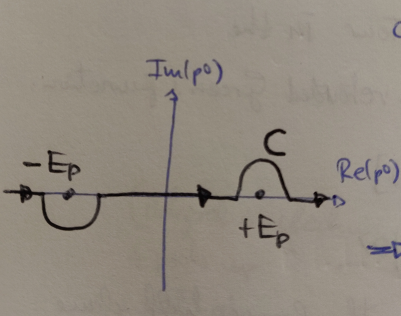
\includegraphics[width=0.3\linewidth]{gfx/Contour1}
	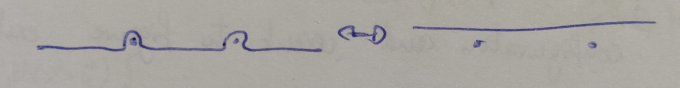
\includegraphics[width=0.7\linewidth]{gfx/Contour2}
	\caption{\itshape Integration contour for Feynman propagator of the real scalar field.}
	\label{fig:contour1}
\end{figure}
with $p^0$ integration along the real axis and with the limit $\epsilon \rightarrow 0$ after performing the integral.
The $i\epsilon$ term represents time ordering. Important is only the position of the poles with respect to the contour, thus the relative position.\\
\textbf{Note that \emph{this} is the place where off-shell contributions come into play since the integral in \ref{eq:feynmanpropagator} is over an unconstrained integration variable $\vec{p} = E_{\vec{p}}$.}

\begin{mybox}{Feynman propagator properties}
Note that the scalar Feynman propagator is symmetric in $x$ and $y$, i.e.
 \begin{equation}
 D_F(x-y) = D_F(y-x), \quad \mathrm{but}\; D(x-y) \neq D(y-x).
 \end{equation}
This will still hold true for interacting vacuum propagators. \textbf{Time ordering maps products of operators onto commuting numbers!} Because of this, expectation values of time ordered operators can
be expressed as path integrals as we will see later.
\end{mybox}
Use
\begin{align*}
	\frac{1}{p^2-m^2+i\epsilon} &= \frac{1}{p^2_0 - \vec{p}^2-m^2 + i\epsilon}=\frac{1}{p^2_0 - (E_p - i\epsilon)^2}\\
	Using \; &\left[-(E_p-i\epsilon)^2 = -E^2_p+2i E_p \epsilon = E^2_p + i \epsilon\right]\; \text{such that we further have} \\
	&= \frac{1}{p_0 - (E_p - \epsilon)} \frac{1}{p_0 +(E_p-i\epsilon)} \\
	\text{two poles at }\quad p_0=E_p -i\epsilon,\quad p_0 =-E_p + i \epsilon
\end{align*}
such that the integration reads as the following along the two possible contours \todo{Insert Feynman contour picture 2}
\begin{align*}
	D_F(x) &= \int \pmeasure \int_{\-\infty}^\infty \frac{\md p^0}{2 \pi} e^{-i p_0 x_0 + i \vec{p}\vec{x}} \frac{i}{p^0-(E_p-i \epsilon)} \frac{1}{p^0 + (E_p - i \epsilon)}\\
	D_F(x) |_{x^0>0} &= \int \pmeasure \underbrace{\frac{(-2 \pi i)}{2 \pi}}_{- \Leftarrow clockwise} \frac{i}{E_p +E_p} e^{-i E_p x^0+ i \vec{p}\vec{x}} = D(x)
\end{align*}
where the description here is equivalent to the Feynman contour with $p^0=-E_p$ and $p^0=E_p$. Therefore, the Feynman propagator is just a Green's function.
\subsubsection{Propagators as Green's functions}
\begin{mybox}{}
	The propagators are Green's functions for the KG equation
	\begin{align*}
		\mathcal{D}(\partial) G(x) &= i \delta(x) \\
		\mathcal{D}(\partial) &= (\partial^2 +m^2) \quad \Rightarrow \quad G(p) = \frac{i}{p^2-m^2},\; i.e.\\
		\mathcal{D}(\partial) D_A(x) &= \mathcal{D}(\partial) D_F(x) = \mathcal{D}(\partial) D_R(x) = -i  \delta(x).
	\end{align*}
Note that the scalar propagator is not a Green's function of the KG but satisfies
\begin{equation*}
	(\partial^2 + m^2) D(x) = 0.
\end{equation*}
\end{mybox}
The Feynman propagator $D_F(x-y)$ is a Green's function for the Klein-Gordon equation:
\begin{equation}
	(\partial^2_x + m^2) D_F(x-y) = -i \delta^{(4)}_D(x-y).
\end{equation}
The Green's function inverts the Klein-Gordon operator.
\begin{enumerate}
		\item
		\begin{figure}[h]
			\centering
			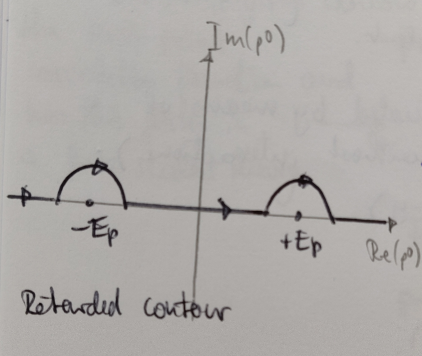
\includegraphics[width=0.7\linewidth]{gfx/Retardedcontour}
			\caption{\itshape Retarded contour.}
			\label{fig:retardedcontour}
		\end{figure} 
	 By avoiding both poles along a contour in the upper half-plane, the solution is the retarded Green's function
		\begin{equation}
			D_R(x-y)=\theta(x^0-y^0) [D(x-y)-D(y-x)]\equiv \theta(x^0-y^0) \expval{[\phi(x),\phi(y)]}{0}.
		\end{equation}
$D_R$ is useful in classical field theory if we know the initial value of some field configuration and want to figure out what it evolves into in the presence of the source.
It propagates information backward in time.
\item 
\begin{figure}[h]
	\centering
	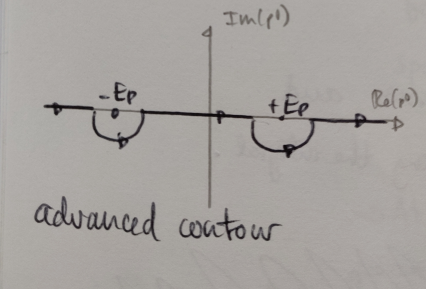
\includegraphics[width=0.7\linewidth]{gfx/Advancedcontour}
	\caption{\itshape Advanced contour.}
	\label{fig:advancedcontour}
\end{figure}
Avoiding both poles $p^0 = \pm \sqrt{E^2_{\vec{p}}}$ in the lower half plane yields the advanced Green's function
\begin{equation}
	D_A (x-y) = \theta(y^0-x^0) [D(x-y)-D(y-x)].
\end{equation}
$D_A$ is useful if we know the end point of a field configuration and want to figure out were it came from. It propagates forward in time.
\item $D_F(x-y)$ propagates positive frequency modes $e^{- i px}$ forward in time and negative frequency modes $e^{ipx}$ backward in time.
\end{enumerate}
Again, the ambiguity of Green’s functions results from an ambiguity in choice of contour when Fourier
transforming $G(p)$. One can write
\begin{equation}
	p^2 -m^2 = (p^0)^2 - E^2_p, \; i.e.\; G(p) = \frac{i}{p^2-m^2}=\frac{i}{(p^0)^2 - \abs{\vec{p}}^2 -m^2} = \frac{i}{(p^0-E_p)(p^0+E_p)}
	\end{equation}
and chose the contour - integrating counterclockwise - pushing both poles in the upper (advanced)
or lower (retarded) half of the complex plane, or pushing $p^0 = E_p$ down and $p^0 = −E_p$ up (Feynman) by
\begin{equation}
G(p) = \lim_{\tilde{\epsilon} \rightarrow 0} \frac{i}{(p^0-(E_p-i \tilde{\epsilon})) (p^0+E_p - i \tilde{\epsilon})}.
\end{equation}
Taking $\epsilon = - i \tilde{\epsilon}^2 + 2 \tilde{\epsilon}E_p$, dropping the quadratic term and ruthlessly switching integration and
limit then gives \ref{eq:feynmanpropagator} with a contour integral. But the contribution away from the real axis vanishes
if we send the contour radius to $\infty$ and close the contour in the lower or upper half appropriately
to the sign of $(x^0 − y^0 )$ because then the integrand falls off
\begin{equation}
\frac{e^{-ip(x-y)}}{p^2-m^2} \stackrel{Im(p^0)\rightarrow \infty}{\longrightarrow}0 \mathrm{\; at\;least\; as\;} e^{-Im(p^0)}.
\end{equation}
The fourth choice in contour, the Keldysh-propagator corresponding to anti-timeordering
\begin{equation}
	\label{eq:keldyshpropagator}
	D_K(x-y) =\theta(y^0-x^0) D(x-y) + \theta(x^0-y^0) D(y-x) = \bra{0}\bar{ \mathcal{T}} \phi(x) \phi(y) \ket{0}
\end{equation}
has no application here and is in fact algebraically dependent on the other three due to the identity
$θ(x^0 − y^0 ) + θ(y^0 − x^0 ) = 1$.

\subsubsection{Causality}
For causality to hold we need to measurements at spacelike distance not ot affect each other. This is guaranteed if any two local observables $O_1(x)$ and $O_2(y)$ at spacelike separation commute, i.e. 
\marginpar{local $\equiv$ local operators only depend on a local neighbourhood of the spacetime point $x$.}
\begin{equation}
\left[O_1(x),O_2(y)\right] \stackrel{!}{=} 0, \quad \mathrm{for} \quad (x-y)^2 < 0,
\end{equation}
even though $D_F (x − y) \neq 0$ for $(x − y)^2 < 0$. More specifically
\begin{equation}
\bra{0} \Delta(x-y) \ket{0} = D(x-y) - D(y-x) =0 \quad for \quad (x-y)^2 <0.
\end{equation}
This ensure that a measurement at $x$ cannot affect a measurement at $y$ when $x$ and $y$ are \emph{not causally connected}.\\
This theory is \emph{indeed causal} with commutators vanishing outside the lightcone 
\begin{align}
	\Delta(x-y)|_{(x-y)^2<0} &= [\phi(x),\phi(y)] |_{(x-y)^2<0} \\
	&= \int \pmeasure \frac{1}{2 E_p} \left[e^{-ip(x-y)} - e^{+i p(x-y)} \right]|_{(x-y)^2<0}=0 \nonumber
\end{align}
\marginpar{The states of QFT are non-local objects.}
because one can always make a Lorentz transformation such that $(x^0-y^0)=0$ for spacelike separation and change the minus sign of the integration variable.
This property will continue to hold in interacting theories, it is usually given as an axiom of local QFTs.\\
Note that the Fourier transformation of the commutator as indicator of free spectrum is
\begin{equation}
\Delta(k) = \frac{\pi}{E_k} \left[\delta(k^0-E_k)- \delta(k^0+E_k)\right]\left[\theta(k^0) - \theta(-k^0)\right].
\end{equation}
The fact that $[\phi(x),\phi(y)]$ is a $\mathbb{C}$-number function, rather than an operator, is a property of \emph{free fields only}.
\subsubsection{Vacuum spectral function and statistical propagator}
\begin{mybox}{}
	With the separation
	\begin{equation*}
		\bra{0}\mathcal{T}\phi (x) \phi(y)  \ket{0} = \half \bra{0} \{\phi(x),\phi(y) \} \ket{0} + \half sgn(x^0-y^0) \bra{0} [\phi(x),\phi(y)] \ket{0}
	\end{equation*}
we can define the spectral function $\rho$ as
\begin{equation}
\label{eq:spectralfunction}
\rho(x-y) :=i \bra{0} [\phi(x),\phi(y)] \ket{0} = i \bra{0} \Delta(x-y) \ket{0},
\end{equation}
and the statistical propagator $F$ as
\begin{equation}
	\label{eq:statisicalpropagator}
	F(x-y):= \half \bra{0} \{\phi(x),\phi(y) \} \ket{0},
\end{equation}
such that
\begin{equation}
	D_F(x-y) = F(x-y) - i\half sgn(x^0-y^0) \rho(x-y).
\end{equation}
\end{mybox}
Note that neither the statistical propagator nor the spectral function is a Green’s function, but
just sums of $D(x)$ such that
\begin{equation*}
	(\square +m^2) \rho (x) = (\square +m^2 ) F(x) = 0.
\end{equation*}
The Fourier transforms of $F$ and $\rho$ can be shown to be proportional to each other
\begin{equation}
	F (p) = ( \half + \delta(p^0)) \rho(p) .
\end{equation}

We will proof this as the special case of zero temperature of the KMS condition much later in the
context of thermal field theory, where it will become clear that $F$ keeps track of the occupation
of states, while $\rho$ keeps track what states exist (i.e. of the spectrum). In vacuum theory, $F$ is
uninteresting because of the above proportionality.


\subsubsection{How to perform the contour integral}
Define a function $g(z)$ with poles $z_0$ and apply Residue theorem:
\begin{equation*}
	g(z) =\frac{1}{E_p+z} e^{-i z (x^0-y^0)}, \quad z_0 =E_p, z=p^0.
\end{equation*}
\begin{align*}
	\Rightarrow \theta(x^0-y^0)&=g(z_0)=\theta(x^0-y^0) \left[\frac{1}{2 \pi i} \oint_{C_1} \frac{g(z) \md z}{z-z_0}\right]\\
	&=\theta(x^0-y^0) \left[\frac{1}{2 \pi i}\oint_{C_1} \left(\frac{1}{E_p+p^0} e^{-i p^0 (x^0-y^0)} \right) \frac{\md p^0}{p^0-E_p}\right] \\
	&= \theta(x^0-y^0) \left[\frac{1}{2 \pi i} \oint_{C_1} \md p^0 \frac{e^{-i p^0(x^0-y^0)}}{(p^0+E_p)(p^0-E_p)}\right] \\
	&=-\theta(x^0-y^0) \frac{1}{2 \pi i} \oint_C \md p^0 \quad \frac{e^{-ip^0(c^0-y^0)}}{(p^0 + E_p)(p^0-E_p)},
\end{align*}
where the minus comes about since the integral is performed clockwise ($\Rightarrow \times (-1)$) and because it picks up the pole at $+E_p \Rightarrow (-1) \times (+1)=-1$.\\
\begin{align*}
	\theta(y^0-x^0) \frac{1}{2 E_p} e^{i E_p (x^0-y^0)} &= \theta(y^0-x^0) g(z_0) \\
	&=\theta(y^0-x^0) \left[\frac{1}{2 \pi i} \oint_{C_2} \left(\frac{1}{p^0+E_p} e^{-i p^0 (x^0-y^0)} \right) \frac{\md p^0}{p^0-E_p}\right] \\
	&= - \theta(y^0-x^0) \frac{1}{2 \pi i} \oint_{C_2} \md p^0 \quad \frac{e^{-i p^0(x^0-y^0)}}{(p^0+E_p)(p^0-E_p)},
\end{align*}
where the minus sign comes about since the integral is performed counter-clockwise ($\Rightarrow \times +1$) and because it picks up pole at $-E_p \Rightarrow +1 \times (-1)=-1$. Thus, the Feynman propagator is given by the addition of both contours
\begin{align*}
	D_F(x-y) &= \int \pmeasure e^{i \vec{p}(\vec{x}-\vec{y})} \left[-\theta(x^0-y^0) \frac{1}{2 \pi i} \oint_{C_1} \md p^0 \frac{e^{-i p^0(x^0-y^0)}}{(p^0+E_p)(p^0-E_p)} \right.\\
	&\left. \qquad - \theta(y^0-x^0) \frac{1}{2 \pi i} \oint_{C_2} \md p^0 \frac{e^{-i p^0(x^0-y^0)}}{(p^0-E_p)(p^0+E_p)}\right]\\
		&\stackrel{R\rightarrow\infty}{=} - \oint \frac{\md^4 p}{(2 \pi)^4} \frac{1}{i} e^{-i p\cdot (x-y)} \underbrace{\left[\theta(x^0-y^0)+\theta(y^0-^0)\right]}_{=1} \frac{1}{(p^0+E_p)(p^0-E_p)} \\
		&= \oint \frac{\md^4 p}{(2 \pi)^4} \underbrace{\frac{i e^{-i p\cdot(x-y)} }{(p^0+E_p)(p^0-E_p)}}_{=p^2-m^2}.
\end{align*}




\newpage





\section{Interacting scalar theory}
\subsection{Introduction}
Our consideration of free scalar field theories showed, that the theory is \emph{exactly solvable}, we can determine the spectrum (Hilbert space is the Fock space of multi-particle states created from the vacuum $\ket{0}$) and the fields have particle excitations which do not interact. Free theories defined an EOM which is linear $(\partial^2+m^2) \phi=0$, which is exactly solved by Fourier analysis (i.e. different modes decouple). It is not possible to solve interacting theory in a closed form, but it is possible by perturbing around the free Lagrangian order by order in interactions, i.e. order by order in loop contributions.\\
\\
Interactions are described in QFT by potentials $V(\phi)$ beyond quadratic order
\begin{equation}
	V(\phi) = \underbrace{\half m^2_0 \phi^2}_{V_0 (\phi)} \qquad + \sum_{n\geq 3} \frac{\lambda_n}{n!} \phi^n.
\end{equation}
The coefficients $\lambda_n$ are called \emph{coupling constants}. Here we restrict ourselves to
\begin{equation}
V(\phi) = \half m^2_0 \phi^2 +\underbrace{\frac{1}{3!} g \phi^3+\frac{1}{4!} \lambda \phi^4}_{V_{\mathrm{int}}},\quad [\lambda_n]=4-n \neq 0 !,
\end{equation}
with the decomposition 
\begin{equation}
	\mathcal{L}=\mathcal{L}_0 +\mathcal{L}_{\mathrm{int}},\quad \mL_{\mathrm{int}}=-V_{\mathrm{int}}, \quad  \mL_{\mathrm{int}}=-\mathcal{H}_{\mathrm{int}},\; H=H_0 +H_{\mathrm{int}}.
\end{equation}
This linear decomposition comes about since we can always separate a theory into a background/free and an interacting solution. Could have different form, but linear decomposition is due to physical requirements:
\begin{enumerate}
	\item Want a local theory, i.e. local interactions $\leftrightarrow$ causality, i.e. \begin{equation}
	\phi^n(x) \in \mL: \qquad \int \int \phi^n(x) \phi^m(y)
	\end{equation}
	would not be local.
	\item $\mL$ has to be a Lorentz scalar, such that we look for terms $\phi^n(x), (\partial \phi)^2, \cancel{\partial \phi \phi^*}$.
	 \item Has to respect internal symmetry of the system. Eg. require $U(1)$ symmetry, then we cannot have $\psi \psi$ terms in $\mL$.
	 \item Renormalizability
	 \begin{equation}
	 	\mL = \left[\half (\partial_\mu \phi) (\partial^\mu \phi) - \half m^2 \phi^2\right] - \frac{\lambda_3}{3!} \phi^3-\frac{\lambda_4}{4!} \phi^4 - \underbrace{\frac{\lambda_5}{5!} \phi^5}_{non-renormalizable, [\lambda_5] <0} + \dots
	 \end{equation}
	 Ignore $\lambda_{n\geq5}$ terms since these theories are not renormalizable in $d=4$. Can always treat non-renormalizable theories as effective theories up to a certain cut-off scale.
\end{enumerate}
Introducing interaction terms leads to changes in the theory:\\
\begin{enumerate}
	\item The Hilbert space is different from the free theory
	\begin{enumerate}
		\item $\ket{0}\leftrightarrow$ vacuum of $H_0:\quad H_0\ket{0} =E_0 \ket{0}$.\\
		  $\ket{\Omega}\leftrightarrow$ vacuum of $H:\quad H\ket{\Omega}=E_{\Omega} \ket{\Omega}$
		with $\ket{\Omega}\neq \ket{0}$ in general.
		\item The mass of the momentum eigenstates of $H$ does no longer equal the parameter $m_0$ that appear in $\mL_0$.
		\item Bound states (e.g. hydrogen) may exist in the spectrum.
		\end{enumerate}
\item The states interact.
\end{enumerate}
The coupling constants are characterized as follows:
\marginpar{Only doing weakly coupled field theories here, because they can be considered as small perturbation of free field theory.}
\begin{enumerate}
	\item $[\lambda_3=g]=1$: The dimensionless parameter is $\lambda_3/E$, $E$ being the energy scale of the process of interest. This means that $\lambda_3 \frac{\phi^3}{3!}$ is a small perturbation at high energies $E\gg \lambda_3$, but a a large perturbation at low energies $E\ll \lambda_3$. Terms that we add to the Lagrangian with this behaviour are called \emph{relevant} because they are most relevant at low energies.
	\item $[\lambda_4=\lambda]=0$: This term is small if $\lambda_4 \ll 1$. Such perturbations are called \emph{marginal}. If $\lambda_4 \ll1$ then perturbation theory is applicable.
	\item $[\lambda_n]<0$ for $n\geq 5$: The dimensionless parameter is $(\lambda_n E^{n-4})$, which is small at low-energies and large at high energies. Such perturbations are called \emph{irrelevant}.
	\item Of the infinite number of interaction terms that we could write down, only $g$,$\lambda$ are needed (for real scalar field, else some more), because the irrelevant couplings become small at low-energies, our field of interest.
\end{enumerate}

\marginpar{Exact solution of non-free QFT is often not possible.}
\begin{mybox}{Lagrangians of interacting scalar field theories}
	\begin{equation}
		\mL = \half (\partial \phi)^2 + V(\phi) \quad V(\phi) = \frac{1}{2 !} m^2_0 \phi^2+ \frac{g}{3!} \phi^3+\frac{\lambda}{4!} \phi^4 + \mO(\phi^5)
	\end{equation}
	$\phi^4$-theory
	\begin{equation}
		\label{eq:lagrangianphi4}
		\mL = \half \left(\partial_\mu \phi \partial^\mu \phi - m^2 \phi^2\right) + \frac{\lambda}{4!} \phi^4,
			\end{equation}
	$\phi^3$-theory
	\begin{equation}
		\label{eq:lagrangianphi3}
		\mL = \half \left(\partial_\mu \phi \partial^\mu - m^2 \phi^2\right) + \frac{g}{3!} \phi^3,
	\end{equation}
	Breit-Wigner theory
	\begin{equation}
		\label{eq:lagrangianBreitWigner}
		\mL = \half \left(\partial_\mu \varphi \partial^\mu \varphi - m^2_{\varphi,0} \varphi^2\right) + \half \left(\partial_\mu \Phi \partial^\mu \Phi-m^2_{\Phi,0} \Phi^2\right) - \frac{\lambda}{2!}\Phi \varphi^2.
	\end{equation}
\end{mybox}
There is a physical justification to ignore $\mO(\phi^5)$ contributions, as we will find out in chapter
4 on renormalization. (Spoiler: its because couplings of $\mO(\phi^5)$ terms are zero in the IR in $\md = 3+1$.)\\
\\
Note that since the potential of $\phi^3$ theory is unbound from below, one does not expect a stable
vacuum to exist (even though quantum effects could in principle change the classical discussion).
However it can be a physical theory in combination with other fields that lead to a stable vacuum
that is bound from below, e.g. $\phi^3+\phi^4$ .




\subsubsection{Two-scalar Lagrangians, examples}
\begin{enumerate}
	\item $\phi^4$ theory:
\begin{equation}
	\mL = \half (\partial_\mu \phi)^2 -\half m^2 \phi^2 - \frac{\lambda}{4!}\phi^4
\end{equation}
with EOM
\begin{equation}
	(\partial^2 + m^2) \phi = - \frac{\lambda}{3!} \phi^3,
\end{equation}
which cannot be solved by Fourier decomposition.\\
\item Scalar Yukawa theory:
\begin{equation}
	\mL = \underbrace{\half \left[(\partial \phi)^2 - m^2 \phi^2\right]}_{KG}+\underbrace{\left[(\partial_\mu \psi^*)(\partial^\mu \psi) - M^2 \psi^*\psi\right]}_{free\,charged\,scalar}  -g  \psi^* \psi \phi.
\end{equation}
\end{enumerate}
\todo{insert 3)	}
\subsubsection{To to study interacting QFTS}
Not exactly solvable in $n>2$ dimensions. There are two possible approaches
\begin{enumerate}
	\item numerical solution, eg lattice gauge theory
	\item Perturbation theory, our approach. It is an expansion around free theory limit and is valid for weak couplings, where small means that that the NLO loop correction scales smaller than LO, since higher orders of the coupling become smaller (lecturer said that strong couplings are defined as $\lambda \geq 1$).
\end{enumerate}






\subsection{Källén-Lehmann spectral representation}
\subsubsection{Hilbert space}
Here we take a look at the spectrum of an interacting real scalar field theory in a manner valid for all types of interactions and without relying on perturbation theory. This representation gives a \emph{general expression} for the time ordered two-point function of an interacting quantum field theory as a sum of free propagators.\\
In interacting theory $[H,\vec{P}]=0$ still holds due  to Lorentz invariance. Their mutual eigenstates $\ket{\lambda_p}$ with
\begin{equation}
	H\ket{\lambda_p}=E_p(\lambda) \ket{\lambda_p}, \quad \vec{P}\ket{\lambda_p} = \vec{p} \ket{\lambda_p}
\end{equation}
correspond via a Lorentz boost to the state at rest, called $\ket{\lambda_0}$.\\
\begin{figure}
	\centering
	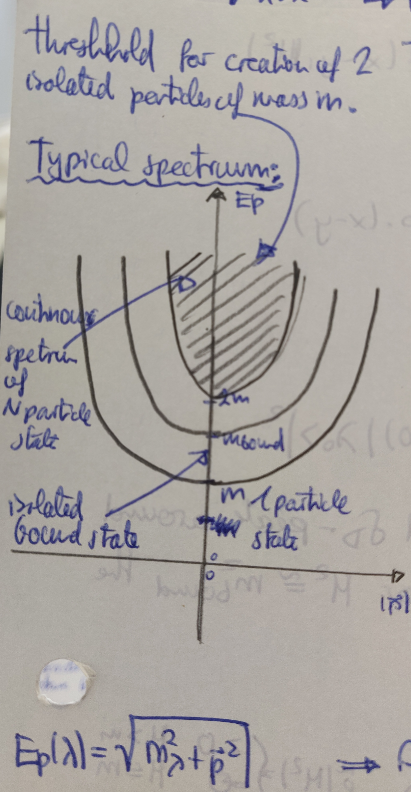
\includegraphics[width=0.7\linewidth]{gfx/Spectruminteractingtheory}
	\caption{\itshape Typical spectrum in the interacting theory.}
	\label{fig:spectruminteractingtheory}
\end{figure}
We can have the following types of $\ket{\lambda_{\vec{p}}}$:
\begin{enumerate}
	\item 1-particle states with $E^2_p = \vec{p}^2+m^2$, they have $p^{\nu}p_{\nu}=m^2$, $m\neq m_0$ (even in vacuum $m \neq m_0$ because of self-interactions).
	\item Bound states with no analogue in the free theory.
	\item 2-and $N$-particle states formed out of 1-particle and the bound states. In this case, we take $\vec{p}$ to the centre-of-mass momentum of the multi-particle state.
\end{enumerate}
\begin{mybox}{Hilbert space of interacting theory}
	Definition of interacting vacuum as Poincaréinvariant state
	\begin{equation}
	\label{eq:vacuumPoincareInvariant}
	U\ket{\Omega}= \ket{\Omega}\quad \forall U\in \mathcal{P}\; \Rightarrow \quad  H\ket{\Omega}=0.
	\end{equation}
	Interacting momentum eigenstates
	\begin{align}
	H\ket{\lambda_{\vec{p}}} &=E_{\vec{p}}(\lambda) \ket{\lambda_{\vec{p}}}\; \mathrm{with}\; E_{\vec{p}}(\lambda) :=\sqrt{\vec{p}^2+m^2_{\lambda}}\\
	\vec{P}\ket{\lambda_{\vec{p}}} &= \vec{p} \ket{\lambda_{\vec{p}}}
	\end{align}
where the single-particle state $\ket{1}_{\vec{p}}$ obeys
\begin{equation}
	P^mu \ket{1_{\vec{p}}}=p^\mu \ket{1_{\vec{p}}} \; with \; p^2=m^2
\end{equation}
with the interacting mass $m$. The interacting momentum eigenstates obey the \emph{completeness} relation
\begin{equation}
	\label{eq:completenessrelation}
	\mI=\ket{\Omega}\bra{\Omega}+ \sum_\lambda\hspace{-0.4cm}\int  \;\int \pmeasure \frac{1}{2 E_p(\lambda)} \ket{\lambda_p} \bra{\lambda_p},
\end{equation}
where $E_p(\lambda)=\sqrt{m^2_{\lambda}+\vec{p}^2}$ and $\sum$ includes a sum over 1-particle states, over all types of bound states as well as over all multiparticle states. $\int \md^3 p \dots$ refer to the centre-of-mass momentum of a state of species $\lambda$.\\
\end{mybox}
\begin{mybox}{Interacting equation of motion}
All these are created from the vacuum $\ket{\Omega}$. The crucial difference to the free theory is, that $ \phi(x)$ cannot simply be written as a superposition of its Fourier amplitudes $a(\vec{p})$ and $a^{\dagger}(\vec{p})$, because $\phi(x)$ \emph{does not obey the free e.o.m}, rather the interacting scalar operator equation of motion
\begin{equation}
	(\partial^2+m^2)\phi^H(x) = j^H(x),
\end{equation}
where generally $j$ is a function of $\phi$. The current can not create single particle states from the
vaccum, i.e.
\begin{equation}
\label{eq:interactingtheoryEOMcurrent}
	\bra{1_p} j(x) \ket{\Omega}=0.
\end{equation}
Thus, acting with  $\phi$ on $\ket{\Omega}$ \emph{does not} simply created a 1-particle state as in the free theory !
\end{mybox}
Proof of \ref{eq:interactingtheoryEOMcurrent}:
\begin{align*}
	\bra{1_p} j(x) \ket{\Omega} &= \bra{1_p} (\partial^2+m^2) \phi(x) \ket{\Omega}\\
	&=\bra{1_p} (\partial^2 +m^2) e^{-i Px} \phi(x) e^{-iPx} \ket{\Omega}\\
	&\stackrel{\ref{eq:vacuumPoincareInvariant}}{=} \bra{1_p}(\partial^2+m^2) e^{iPx} \phi(0) \ket{\Omega}\\
	&=\bra{1_p}(-P^2+m^2) e^{iPx} \phi(0) \ket{\Omega} \\
	&= \bra{1_p}(-p^2+m^2) e^{iPx} \phi(0) \ket{\Omega}\\
	&=\bra{1_p}(-p^2+m^2) \phi(x)\ket{\Omega}\\
	&=0.
\end{align*}
An aside (Reh-Schlieder property): local operators can not have an identically vanishing vacuum product, i.e.
\begin{equation}
	\label{eq:rehschlieder}
	\mO(x) \ket{\Omega} =0 \quad \Leftrightarrow \;\mO  =\hat{ 0}.
\end{equation}
\subsubsection{Propagator}
\begin{mybox}{Propagator interacting theory}
\begin{align}
	D(x-y)&:=\bra{\Omega}\phi(x)\phi(y)\ket{\Omega} \\
	&=\sum_\lambda \hspace{-0.4cm}\int \;\abs{\bra{\Omega}\phi(0)\ket{\lambda_0}}^2 \int \pmeasure \frac{1}{2 E_p} e^{-ip(x-y)}.\nonumber
\end{align}
\end{mybox}
\begin{mybox}{Feynman-propagator in interacting scalar theory}
We find the time-ordered interacting Feynman-propagator to be
\begin{align}
\expval{T\phi(x)\phi(y)}{\Omega} = \sum_{\lambda} \int& \frac{\md^4 p}{(2 \pi)^4} \frac{i}{p^2-m^2_{\lambda} +i\epsilon}\\
& e^{- i \cdot (x-y)} |\bra{\Omega}\phi(0)\ket{\lambda_0}|^2\nonumber,
\end{align}
or, equivalently, it turns out that in \emph{any} Lorentz-invariant theory we can
write the $2$-point function in the Kallén-Lehmann spectral representation as:
\begin{equation}
	\expval{T\phi(x)\phi(y)}{\Omega} = \int_0^{\infty} \frac{\md M^2}{2 \pi} \quad \rho(M^2) D_F(x-y,M^2),
\end{equation}
where we defined the Feynman propagator for a \emph{free} quantum field of mass $M$
\begin{equation}
	D_F(x-y, M^2) = \int \frac{\md^4 p}{(2 \pi)^4} \frac{i}{p^2-M^2+i\epsilon} e^{-i p\cdot (x-y)} 
\end{equation}
and the \emph{spectral function} (density)
\begin{equation}
	\rho(M^2) = \sum_{\lambda} 2 \pi \delta_D(M^2-m^2_{\lambda}) |\bra{\Omega} \phi(0) \ket{\lambda_0}|^2,
\end{equation}
which roughly speaking says "what are the masses of states that $\phi$ is creating
from the vacuum?”
\end{mybox}
In a free theory with mass $m^2$, the spectral density would read
\begin{equation*}
	\rho_{free}(M^2) = 2\pi \delta (m^2-M^2)
\end{equation*}
such that in the free theory the field $\phi$ just creates particles of mass $m$ as a Delta peak for $M^2=m^2$. For interacting theory however, we get a spectrum above the one-particle delta peak
\begin{equation*}
	\rho_{int}(M^2) = 2 \pi Z \delta (m^2-M^2) + stuff
\end{equation*}
note that the weight of the delta function has changed: as you now have some other probability to make
other things, the probability to create the single-particle state has been reduced.
We now have a non-vanishing probability to get higher than $1$-particle states via scattering, i.e. probability $p$ to create single particle $p\propto Z<1$, compare \ref{fig:spectruminteractingtheorymass}.\\
Note that whenever $Z$ is finite, it is at least true that we still create a particle. What if $Z$ drops to zero?
Then there is no probability that the φ field will create a physical particle. This is what happens in QCD
due to confinement.
\subsubsection{Self-energy}
\begin{mybox}{Self-energy and Dyson-Schwinger equation}
	The self energy  $−iM^2$ is the regular part of the RHS of the e.o.m. of the Feynman propagator
	\begin{equation}
		(\square_x+m^2)D_F(x,y)=:-i\delta(x-y) + i \int \md^4 z M^2(x,z)D_F(z,y)
	\end{equation}
	expressing the self-energy in terms of $j$ as defined by \ref{eq:interactingtheoryEOMcurrent} $(\square + m^2 ) \expval{\phi} = \expval{j}$
	\begin{equation}
	\label{eq:selfenergyCurrent}
		i \int \md^4z M^2(x, z)D_F (z, y) = \langle \mathcal{T} j(x)\phi(y)\rangle − \expval{j(x)} \expval{\phi(y)}
			\end{equation}
			allows for an operator evolution equation for the Feynman propagator that is closed in $\phi^{(H)}$, the
			Dyson-Schwinger equation (in compact integral notation)
			\begin{equation}
				\label{eq:dysonschwingereq}
				D_F = D^{(0)}_F + D^{(0)}_F (-i M^2) D_F.
			\end{equation}
\end{mybox}
Proof of \ref{eq:selfenergyCurrent}:\\
\begin{align*}
	&(\square_x+m^2)D_F(x,y) = (\square_x+m^2) \\
	&\times \left[\half \bra{0}\{\phi(x),\phi(y)\} \ket{0} + \half sgn(x^0-y^0) \bra{0}[\phi(x),\phi(y)]\ket{0} \right].
\end{align*}
The tricky term is now of course the $x^0$-derivative of the product sgn$(x^0-y^0)\rho(x,y)$
\begin{equation*}
	\partial^2_{x^0} sgn(x^0-y^0) \rho(x,y)=
\end{equation*}
with this we have
\begin{align*}
	(\square_x+m^2) D_F(x,y) &= -i \delta(x-y) + \half \expval{\{j(x),\phi(y)\}} \\
	&+ \half sgn(x^0-y^0) \expval{[j(x),\phi(y)]} - \expval{j(x)} \expval{\phi(y)}\\
	&=-i\delta(x-y) + \expval{\mathcal{T}j(x) \phi(y)} - \expval{j(x)} \expval{\phi(y)}
\end{align*}
i.e. we can express the self energy as
\begin{equation*}
	i \int \md^4 z M^2(x,z) D_F(z,y) = \expval{\mathcal{T} j(x) \phi(y)} - \expval{j(x)} \expval{\phi(y)}. \quad \blacksquare
\end{equation*}

\subsubsection{Wavefunction renormalization and spectrum of states via self energy}
\begin{mybox}{}
	We define
	\begin{equation}
		\label{eq:wavefunctionrenormalization}
		Z:= \abs{\bra{1_{\vec{0}} } \phi(0) \ket{\Omega}}^2
	\end{equation}
	and find that
	\begin{equation}
	\label{eq:statesWavefunctionRenorm}
	\bra{1_{\vec{p}} }\phi(x) \ket{\Omega} = \sqrt{Z} e^{ipx} |_{p_0 = E_{\vec{p}}},
	\end{equation}
	i.e. $Z$ is the probability for $\phi(x)$ to create a $1$-particle state from the interacting vacuum.\\
	$Z$ is a measure for the strength of the interaction with $0\leq Z\leq 1$ and
	\begin{equation}
		Z=1 \Leftrightarrow j(x) = \hat{ 0}\Leftrightarrow \rho(\mu^2) = \delta(\mu^2-m^2) \;\Leftrightarrow\; \mathrm{free\;theory}.
	\end{equation}
	$Z$ therefore takes as a rescale factor the effects of interactions or quantum fields into account,
	where $\ket{1_0}$ is the 1-particle state at rest.
\end{mybox}
In general we have
\begin{equation}
	\bra{\lambda\vp }\phi(x) \ket{\Omega} = \bra{\lambda_{\vec{0}}} \phi(0) \ket{\Omega} e^{ipx} |_{p_0 = E\vp(\lambda)}.
\end{equation}
Proof:\\
\begin{align*}
	\bra{\lambda\vp}\phi(x) \ket{\Omega} &= \bra{\lambda_{\vec{p}}}e^{iPx} \phi(0) e^{-iPx} \ket{\Omega}\\
	&= \bra{\lambda_{\vec{p}}} e^{iPx} \phi(0) \Omega \\
	&= \ket{\lambda_{\vec{p}}} \phi(0) \ket{\Omega} e^{ipx} |_{p_0 = E_p(\lambda)}\\
	&= \bra{\lambda_{\vec{p}}} U^{-1} \phi(0) U \ket{\Omega} e^{ipx} |_{p_0=E\vp(\lambda)}\\
	&= \bra{\lambda_{\vec{p}}} U^{-1} \phi(0) \ket{\Omega} e^{ipx} |_{p_0 =E\vp(\lambda)}\\
	&=\bra{\lambda\vz} \phi(0) \ket{\Omega} e^{ipx} |_{p_0 =E\vp(\lambda)}.
\end{align*}
For fields with spin, the wavefunction renormalization remains a Lorentz scalar, e.g.
\begin{align}
	Z_\phi &= \bra{1\vz}\phi(0) \ket{\Omega}\bra{\Omega}\phi(0) \ket{1\vz}\\
	Z_\psi &= \bra{1\vz}\bra{\psi}^A(0)\ket{\Omega} \bra{\Omega}\psi_A(0) \ket{1\vz}\\
	Z_A &= \bra{1\vz} A^\mu(0) \ket{\Omega}\bra{\Omega} A_\mu(0) \ket{1\vz}.
\end{align}
\begin{figure}[h!]
	\centering
	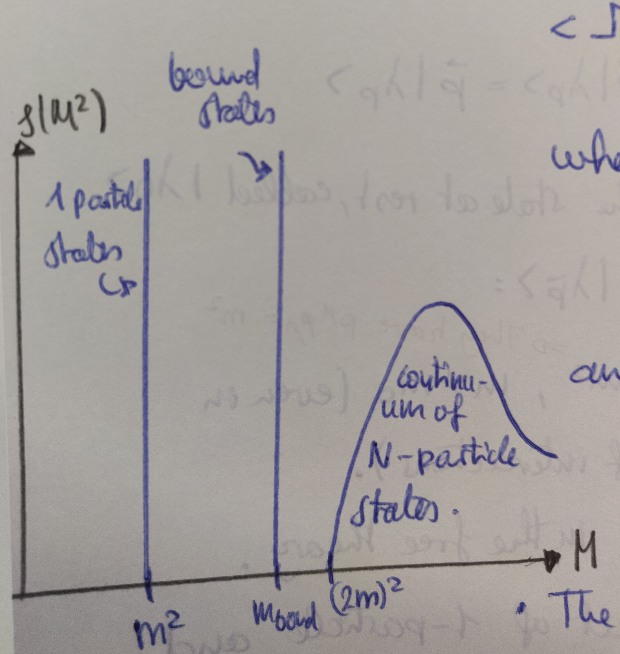
\includegraphics[width=0.7\linewidth]{gfx/SpectrumInteractingTheoryMass}
	\caption{\itshape Particle spectrum with respect to the mass.}
	\label{fig:spectruminteractingtheorymass}
\end{figure}
The 1-particle state lead to an isolated $\delta_D$-peak around $M^2=m^2$. Therefore, below $M^2\approx(2m)^2$ or $M^2\approx m^2_{\mathrm{bound}}$ the spetral function takes the form
\marginpar{In general $\int_0^{\infty} \frac{\md M^2}{2 \pi} \rho(M^2)=1$ holds.}
\begin{align}
	\rho(M^2) &= 2 \pi \delta_D(M^2-m^2) \quad Z \\
	&= 2 \pi \delta_D(M^2-m^2) Z+ \tilde{\rho}(M^2), \quad \tilde{\rho} (M^2) \left\{ \begin{array}{lr} \geq 0 & M>m \\
		=0 & M \leq m.
	\end{array}\right\}
\end{align}
with the \emph{wavefunction renormalization} $Z$ which takes as a rescale factor the effects of interactions or quantum fields into account
\begin{equation}
	Z=|\bra{\Omega}\phi(0)\ket{1_0}|^2,
\end{equation}
where $\ket{1_0}$ is the 1-particle state at rest.
\\
\\
We find the following statements 
\begin{enumerate}
	\item
	\marginpar{Calculation of the propagator yields the mass of the particle !}  The 1-particle state is the first analytic pole of the fully Feynman propagator at $m^2 \Rightarrow$ The mass-square $m^2$ of the particle is the location of the lowest-lying pole of the Fourier transformed propagator.
	\item Bound states appear at higher isolated poles
	\item N-particle states give rise to a branch cut beginning at $p^2=em^4$.
\end{enumerate}
The field strength renormalization in a free theory, i.e. $Z=1$, because $\phi(0)$ just creates the free particle from vacuum. In an interacting theory
\begin{equation}
	1 > \sqrt{Z} = \quad |\bra{\Omega} \phi(0) \ket{1_0}|,
\end{equation}
because $\phi$ creates not only 1-particle states and thus the overlap with the 1-particle states is smaller. Thus,
\begin{statements}
	$Z=1$ if and only if the theory is free.
\end{statements}
\begin{mybox}{Källen-Lehman spectral representation and mass gaps}
	\begin{align}
		&\int \md^4 x \bra{\Omega}\mathcal{T} \phi(x) \phi(y) \ket{\Omega} e^{ip(x-y)} \\
		&= \int_0^\infty \md \mu^2 \rho( \mu^2) \frac{i}{p^2-\mu^2+i\epsilon}\nonumber \\
		\mathrm{with}\; &\;\rho(\mu^2) := \sum_\lambda \hspace{-0.4cm}\int \; \abs{\bra{\Omega} \phi(0) \ket{\lambda_{\vec{0}}}}^2\delta(\mu^2-m^2_\lambda)
	\end{align}
where the spectral function is normalized
\begin{equation}
	\int \md \mu^2 \rho(\mu^2) =1.
\end{equation}
A theory is said to have a \emph{mass gap} if there exists and $ M^2>0$ such that (compare \ref{fig:spectruminteractingtheorymass})
\begin{equation}
\label{eq:massgap}
\rho(\mu^2) = Z \delta(\mu^2-m^2) + \rho_c(\mu^2) \;\; \mathrm{with}\; \rho_c=0 \;\mathrm{for} \; \mu^2 < M^2.
\end{equation}
A typical size for such an $M$ is the two particle bound state mass $M\approx 2m$. Another way of phrasing this in terms of the spectrum of the Hamiltonian
\begin{equation}
	H \ket{\psi} = E_\lambda \ket{\psi}\; \mathrm{with}\; E_\lambda \in \{0,[M,\infty) \} \quad \mathrm{with}\; M>0.
\end{equation}
If a theory possesses a mass gap, we can \emph{define the interacting mass} $m$ in terms of Källen-Lehmann spectral representation as the pole mass of the spectral function
\begin{align}
	\label{eq:polemassKLrep}
	\int \md^4x\bra{\Omega}\mathcal{T}\phi(x) \phi(y) \ket{\Omega}e^{ip(x-y)} &\stackrel{!}{=} \frac{iZ}{p^2-m^2+i \epsilon} \\
	&+ \int_{M^2}^\infty \md \mu^2\rho(\mu^2) \frac{i}{p^2-\mu^2+i\epsilon}.
\end{align}
\end{mybox}
Theories without a mass gap are generally believed to be unphysical, even though there is a lot of physical use for conformal theories which do not possess a mass gap.\\
\\
In the derivation of the interacting Feynman propagator we made use of the transformation behaviour of a scalar field under a Lorentz transformation
\begin{equation}
	x \mapsto x'=\Lambda x \quad \Rightarrow \quad U^{-1}(\Lambda)\phi(x') U(\Lambda) = \phi(x),
\end{equation}
because classically $\phi(x) \mapsto \phi'(x')=\phi(x)$ has its analogue in 
\begin{equation}
	\Leftrightarrow \bra{\alpha'} \phi(x') \ket{\beta'} = \bra{\alpha} \phi(x)\ket{\beta}=\bra{\alpha}U^{-1} \phi(x')U\ket{\beta}.
\end{equation}

\subsection{S-matrix and asymptotic in/out-states}
In interacting theory, the ladder operators in the mode expansion of the fields are now also time dependent, a simple canonical quantization via equal time commutation relations inducing time slices is not possible any more. This comes about since the interacting quantum field obeys an equation of motion 
\begin{equation}
	(\partial^2+m^2)\phi(x)=j(x)
\end{equation}
with source $j(x)$. On a technical note, these constructions have in practice to be done via wavepackets in order to guarantee bounded operators, i.e
 \begin{equation*}
 f_1(\vec{k}) \propto \exp\left[-\frac{(\vec{k}-\vec{k}_1)^2}{4 \sigma^2}\right] \quad \Rightarrow \; a^\dagger_1 \equiv \int \md^3 k f_1(\vec{k}) a^\dagger_{\vec{k}}.
 \end{equation*}
\subsubsection{In- and out Fock spaces and states}
\marginpar{Can be derived in the interaction picture as well, but here with in \& out states.}
Consider scattering of incoming states $\ket{\alpha,in}$ to outgoing states $\ket{\beta,out}$ with the aim of computing the QM transition amplitude, i.e. the probability amplitude for scattering of $\ket{\alpha,in}$ to $\ket{\beta,out}$.
\begin{mybox}{In and out states}
	Associated to the in and out states are the in and out field operators $\phi_{in}, \phi_{out}$, which satisfy
	\begin{equation}
		\partial^2+\underbrace{m^2}_{\neq m^2_0}  \phi_{in, out} (x) = 0 \quad \textcolor{red}{!}
	\end{equation}
	They have the same equal time commutation relations
	\begin{equation}
		[\phi_{in, out}(x),\Pi_{in,out} (y)]_{x^0=y^0} = i \delta^{(3)}_D (\vec{x}-\vec{y}),
	\end{equation}
	with others vanishing.
\end{mybox}
Associated to the in and out fields are two sets of creation and annihilation operators, $a^{\dagger}_{in}(\vec{p}), a_{in}(\vec{p}), a^{\dagger}_{out}(\vec{p}),a_{out}(\vec{p})$, acting in the same Hilbert space, on two complete sets (Fock spaces, initial $\mathcal{F}_{in}$ and final space $\mathcal{F}_{out}$). These operators satisfy the commutation relations
\begin{equation}
	[a_{in,out}(\vec{p}) , a^{\dagger}_{in,out} (\vec{p})]= i \delta_D(\vec{p}-\vec{p}'),
\end{equation}
with others vanishing.\\
The action of the creation operators on the respective vacua and states with a finite number of particles in the in and out states is given by
\begin{align}
	\ket{in, q_1, \dots,q_n} &=a^{\dagger}_{in}(\vec{q}_1) \dots a^{\dagger}_{in} (\vec{q}_n) \ket{\Omega,in}\\
	\ket{p_1,\dots, p_n, out} &= a^{\dagger}(\vec{p}_1) \dots a^{\dagger}(\vec{p}_n) \ket{\Omega,out}\\
	\mathcal{H}_i &= \mathrm{span}\{\ket{in, q_1,\dots, q_n}\}\\
	\mathcal{H}_f &= \mathrm{span}\{\ket{out,p_1,\dots,p_n}\},
\end{align}
where issues of normalization have been ignored!
\begin{mybox}{Relation between free vacuum $\ket{0}$ and interacting vacuum$\ket{\Omega}$}
		\begin{equation}
			\ket{0,in}=\ket{0,out} = \ket{\Omega}.
		\end{equation}
\end{mybox}
In the \emph{asymptotic past}, $t\rightarrow-\infty$, the in-states $\ket{i, in}$ are described as distinct wave packets corresponding to well-separated single particle states. Being far apart for $t\rightarrow-\infty$, they travel freely as individual states.\\
As these states approach each other, they start to interact and scatter into the final states. For $t\rightarrow\infty$ these final states are again asymptotically free and well-separated 1-particle states.
\begin{mybox}{}
	\begin{equation}
		\ket{\Omega;in} = \ket{\Omega;out} = \ket{\Omega}
	\end{equation}
	\begin{align}
		\phi_{in}(x) &= \int \pmeasure \frac{1}{\sqrt{2 E\vp}} \left(a_{in}(\vec{p}) e^{-ipx} +a^\dagger_{in}(\vec{p}) e^{ipx}\right) \\
		& \mathrm{with}\; E\vp=\sqrt{\vec{p}^2 +m^2},\; m\neq m_0\nonumber
	\end{align}
	with $\phi_{in}$ and $a_{in}$ obeying all the free commutation relations and therefore
	\begin{align}
		a^\dagger_{in}(\vec{p}) &= -\frac{i}{2 E\vp} \int \md^3 x e^{-ipx} \stackrel{\leftrightarrow}{\partial_0} \phi_{in}(x)\\
		\ket{p_i;in} &= \sqrt{2 E_{\vec{p}_i}} a^\dagger_{in} (\vec{p}_i)\ket{\Omega},
	\end{align}
and additionally the important relation
\begin{equation}
	\lim_{t\rightarrow-\infty} \bra{\alpha;out}\phi_{in}(x) \ket{\beta; in} = \frac{1}{\sqrt{Z}} \lim_{t\rightarrow-\infty} \bra{\alpha;out}\phi(x) \ket{\beta;in}
\end{equation}
that says that in the infinite past and future the theory behaves as if it was free. Relation \ref{eq:statesWavefunctionRenorm} can be expressed as
\begin{equation}
\bra{1\vp}\phi_{in}(x) \ket{\Omega} = \frac{1}{\sqrt{Z}} \bra{1\vp} \phi(x) \ket{\Omega} = e^{ipx}|_{p_0=E\vp}.
\end{equation}
All these relations are true also for the out-field with obvious replacements.
\end{mybox}
We can expand
\begin{equation}
	\phi_{in}(x) = \int \pmeasure \frac{1}{\sqrt{2 E_p}} \left[a_{in}(\vec{p}) e^{- i p\cdot x} +a^{\dagger}_{in} (\vec{p}) e^{i p\cdot x}\right].
\end{equation}
We can identify
\begin{equation}
	\lim_{t\rightarrow - \infty} \bra{\alpha}\phi\ket{\beta} = \lim_{t\rightarrow - \infty} \sqrt{Z} \bra{\alpha}\phi_{in} \ket{\beta} \; \Leftrightarrow\; \begin{array}{lr}
	\bra{\alpha}\phi \ket{\beta} \stackrel{t \rightarrow - \infty}{\rightarrow} \sqrt{Z} \bra{\alpha}\phi_{in} \ket{\beta} \\
	\bra{\alpha}\phi \ket{\beta} \stackrel{t\rightarrow +\infty}{\rightarrow} \sqrt{Z} \bra{\alpha} \phi_{out} \ket{\beta}
	\end{array}.
\end{equation}
\subsubsection{Examples for asymptotic states in scalar theory}
\begin{enumerate}
	\item \begin{equation}
		\mL =\mL_{KG} - U(x) \phi \quad \Leftrightarrow \quad (\partial^2 +m^2) \phi=- U(x),
	\end{equation}
	which describes scattering in an external potential. At $t=\pm\infty$, particles are far away from $U(x)$ if is falls off at $\infty\Rightarrow \ket{i},\ket{f}$ are eigenstates of $H_0$.
	\item \begin{equation}
		\mL = \mL_{KG} - \frac{\lambda}{4!} \phi^4 \quad \Leftrightarrow\quad (\partial^2+m^2) \phi= - \frac{\lambda}{3} \phi^3,
	\end{equation}
	which describes scattering in a \emph{dynamical potential}. Even at $t=\pm \infty$, can't turn off $H_{int}$, since the field is everywhere in space and time. However, even though a asymptotic they are never free states.
\end{enumerate}
In the end, problem is to calculate $\bra{f}S\ket{i}$ with $\ket{i,f}$ eigenstates of the free theory. 

\subsubsection{The S-matrix and the scattering process}
\begin{mybox}{The S-matrix}
	The S-matrix (scattering) maps the out-states onto the in-states (because the Fock spaces are isomorphic):
	\begin{equation}
		\ket{\alpha, in} = \quad S\ket{\alpha, out}, \;\Rightarrow S(\alpha,\beta):= \bra{\beta;out} S\ket{\alpha;out} = \bra{\beta;out}\ket{\alpha;in}
	\end{equation}
	with the properties
	\begin{enumerate}
		\item S is unitary $S^{\dagger} = S^{-1}$,
		\item $\phi_{in}(x) = \quad S \phi_{out}(x) S^{-1}$,
		\item $\ket{vac, in} =\ket{vac, out} = \ket{\Omega}$ and $S\ket{\Omega}=\ket{\Omega}$.
		\item $\phi_{in}(x) = S\phi_{out}(x) S^\dagger$
	\end{enumerate}
where the $\alpha$ and $\beta$ labels are usually chosen as momenta.
Thus, 
\begin{equation}
	S_{fi} = \lim_{t_{\pm} \rightarrow\pm \infty} \bra{f(t_+)} U(t_+,t_-) \ket{i(t_-)}_I \equiv \bra{f}S\ket{i},
\end{equation}
and
\begin{equation}
P(i\rightarrow f) =|\bra{f,in}S\ket{i,in}|^2 
\end{equation}
\emph{is the probability for scattering from initial states to the final states !}.\\
The vacuum is invariant $S\ket{\Omega}=\ket{\Omega}$.
\end{mybox}
Formally, the scattering process is described  by the following:\\
We have one Hilbert space for the whole scattering process from $t=-\infty$ to $t=+\infty$. There exist two Fock spaces $\mathcal{F}_{in}, \mathcal{F}_{out}$ in this Hilbert space, they are not disjoint because states can simply not participate in the scattering process. Long before the collisions, i.e. in the asymptotic past, we have well separated, free and independent wavepackets, the $\ket{\alpha,in}$ states with $\mathcal{F}_{in}=\mathrm{span}\{\ket{\alpha,in}\}$. Long after the collisions, we again have well separated, free and independent wavepackets, the $\ket{\beta,out}$ states with $\mathcal{F}_{out} = \mathrm{span}\{\ket{\beta,out}\}$. Then there exists an isomorphism between $\ket{\alpha,in}$ and $\ket{\beta,out}$, the $S$-matrix, with
\marginpar{$\mathcal{H}=\mathcal{F}_{out} \cup \mathcal{F}_{in}, \mathcal{F}_{out} \cap \mathcal{F}_{in} \neq \emptyset$.}
\begin{equation}
	\ket{\alpha, in}=S\ket{\alpha,out}, \qquad S:\mathcal{F}_{out} \rightarrow \mathcal{F}_{in}.
	\end{equation}
Then again, $\mathcal{F}_{in}=\mathrm{span}\{\ket{\alpha,in} = \phi_{in}(x)\ket{\Omega,in}\}$ and $\mathcal{F}_{out}=\mathrm{span}\{\ket{\beta,out}= \phi_{out}(x) \ket{\Omega,out}\}$ with $\ket{\Omega,in} = \ket{\Omega,out}=\ket{\Omega}$.\\
We thus find
\begin{align}
	S_{\beta \alpha} &:= \braket{\beta,out}{\alpha,in}, \qquad \ket{\alpha,in} = \sum_{\beta} S_{\beta \alpha} \ket{\beta,out}\\
	\Rightarrow \hat{S}\ket{\alpha,out} &=\sum_{\beta} S_{\beta \alpha} \ket{\beta,out} = \ket{\alpha,in} \\
	\Rightarrow S_{\beta \alpha} &= \braket{\beta,out}{\alpha,in} = \bra{\beta,out} \hat{S}\ket{\alpha,out}\\
	\bra{\beta,out}S^{\dagger} &= \bra{\beta,in} \qquad SS^{\dagger}=\sum_{\beta} \ket{\beta,in}\bra{\beta,in} = \mathcal{I}.
\end{align}
The probability amplitude for scattering from initial to final state.
\begin{mybox}{$T$-Matrix and Feynman amplitude $M$}
	$T$-matrix
	\begin{equation}
		\label{eq:tmatrix}
		\bra{f}S\ket{i} =: \delta_{fi} + T_{fi}.
	\end{equation}
	We will express the $\delta_{fi}$ more explicitly as the disconnected part of the $S$-matrix by LSZ reduction.\\
	Feynman amplitude $M$
	\begin{align}
		\bra{f}S\ket{i} &=: \delta_{fi} + i (2\pi)^4 \delta(p_f-p_i)M_{fi} \\
		i.e.\; T_{fi} &= i (2\pi)^4 \delta(p_f-p_i) M_{fi}.
	\end{align}
\end{mybox}
\begin{mybox}{optical theorem}
	Unitarity of the $S$ matrix immediately implies that
	\begin{equation}
	\label{eq:tmatrixunitarity}
		T^\dagger T = - i(T-T^\dagger)
	\end{equation}
	evaluating this equation in a free momentum eigenbasis by inserting a full set of states gives
	\begin{align}
		2 \mathrm{Im}M_{fi} &=\sum_{n=1}^\infty \left(\prod_{j=1}^{n} \int \frac{\md^3 q_j}{(2 \pi)^3} \frac{1}{2 E_{\vec{q}_j}} \right)\\
		&(2 \pi)^4  \delta(p_i -\sum_j q_j) M^*(f\rightarrow \{q_j\} ) M(i\rightarrow\{q_j\}) \nonumber
	\end{align}
which relates the imaginary part of an arbitrary scattering process to the product of two-scattering processes. One factor process goes from $i\rightarrow \{q_i\}$ and the other from $\{q_i\} \rightarrow f$ and they are contracted by a phase space integral over all possible intermediate states $\{q_i\}$.
\end{mybox}
This establishes \emph{cutting rules} for Feynman diagrams, which we will discuss under momentum Feynman rules.\\
In generic labels \ref{eq:tmatrixunitarity} implies for the diagonal elements of $T^\dagger T$
\begin{equation}
	\sum_\alpha \abs{T_{\alpha \beta}}^2 = 2 \mathrm{Im}T_{\beta  \beta}.
\end{equation}
This relates the \emph{total cross section} to the \emph{forward scattering amplitude}, because in a momentum basis $\mathrm{Im}T_{\beta\beta}\propto \mathrm{Im}M(k_i\rightarrow k_i)$ and $T^\dagger T\propto \sigma(k_i \rightarrow \mathrm{\;all\;possible\;final\;states})$.\\
\\
In S-matrix theory, the cluster decomposition principle states that if multi-particle processes $\alpha_1\rightarrow\beta_1,\dots,\alpha_N\rightarrow\beta_N$ are studied in $N$ very distant laboratories, then the S-matrix element for the overall process factorizes
\begin{equation*}
	S_{\beta_1+\dots + \beta_N,\alpha_1+\dots+\alpha_N}\rightarrow S_{\beta_1 \alpha_1} \dots S_{\beta_N \alpha_N} 
\end{equation*}
if for all $i\neq j$, all of the particles in states $\alpha_i$ and $\beta_i$ are at great spatial distance from all of the particles in states $\alpha_j$ and $\beta_j$.

\subsection{The LSZ reduction formular}
\marginpar{As it is always the case for in and out states we regard the fully interacting theory, $\ket{\Omega}$.}
\begin{mybox}{The LSZ reduction formular}
The aim is to compute a S-matrix element $\braket{p_1,\dots,p_n,out}{q_1,\dots,q_r,in}$ for a real scalar field. Note that $p_1,\dots,p_n$ and $q_1,\dots,q_r$ are \emph{on-shell} since they correspond to the physical 4-momentum of the out-and incoming 1-particle states. We find

\begin{align}
&\bra{p_1,\dots,p_n;in}T\ket{q_1,\dots,q_r;in} = \\
&\prod_{k=1}^{n} \int \md^4 y_k e^{ip_k y_k} \prod_{l=1}^{r} \int \md^4 x_l e^{-iq_l x_l}\nonumber \\
&\cdot (\square_{y_1} +m^2) \dots (\square_{y_n} + m^2)(\square_{x_1} +m^2) \dots (\square_{x_n}+m^2)\nonumber \\
&\qquad  \bra{\Omega}\mathcal{T}\prod_{k=1}^n \phi(y_k) \prod_{l=1}^{r} \phi(x_l) \ket{\Omega}\nonumber
\end{align}
such that the Lemann-Symanzik-Zimmerman (LSZ) formula reads
\begin{align}
	\label{eq:lszformula}
	&\bra{p_1,\dots,p_n;in}T\ket{q_1,\dots,q_r;in} =\\
	& \left(\prod_{k=1}^{n} \frac{p^2_k-m^2}{i\sqrt{Z}} \right) \left(\prod_{l=1}^{r} \frac{q^2_l-m^2}{i\sqrt{Z}}\right)|_{p^2_k=q^2_l=m^2}\nonumber \\
	&\prod_{k=1 }^{n} \int\md^4 y_k e^{ip_k y_k} \prod_{l=1}^{r} \int \md^4 x_l e^{-i q_l x_l}\bra{\Omega} \mathcal{T}\prod_{k=1}^{n}\phi(y_k) \nonumber \\
	&\prod_{l=1}^{r} \phi(x_l) \ket{\Omega}|_{p^2_k=q^2_l=m^2}\nonumber
\end{align}
i.e. the connected S-matrix elements of $n$ to $m$ particles scattering are the coefficients of the multi-particle pole of the Fourier transformed $(n+m)$-point correlation function. The poles are where  the momenta are on-shell, i.e. the physical mass.
\end{mybox}
\marginpar{
	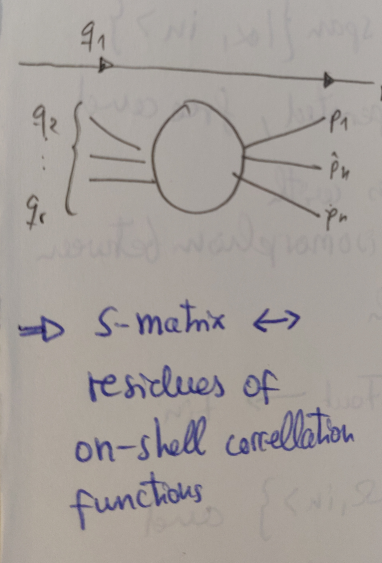
\includegraphics[width=0.3\marginparwidth]{gfx/disconnectediagram}
	\captionof{figure}{\itshape Disconnected diagram}
		\label{fig:disconnectediagram}
}
Because 
This LSZ-formula reduces the computation of the S-matrix to the computation of time-ordered correlation functions\\ $\expval{T\phi(y_1) \dots \phi(y_n) \phi(x_1)\dots \phi(x_n)}{\Omega}$ of the full interacting theory.\\
The first term describes a process where on of the in-and outgoing states are identical and do not participate in scattering.
Such an amplitude corresponds to a disconnected diagram, compare fig. \ref{fig:disconnectediagram}, and its computation reduces to computing an S-matrix element involving only $(r-1)$ in-and $(n-1)$ out-states.\\
For the connected term we find equivalently
\begin{align*}
	&\prod_{k=1}^{n} \int_{\mR^{3,1}} \md^4y_k e^{i p_k \cdot y_k} \prod_{l=1}^{r} \int_{\mR^{3,1}} \md^4x_l e^{-i q_l \cdot x_k}  \times \expval{T\prod_k \phi(y_k) \prod_l \phi(x_l)}{\Omega}\\
	&= \left(\prod_{k=1}^n \frac{i \sqrt{Z}}{p^2_k-m^2}\right) \left(\prod_{l=1}^{r} \frac{i \sqrt{Z}}{q^2_l - m^2}\right) \times \bra{p_1,\dots,p_n}S\ket{q_1,\dots,q_r}  |_{\mathrm{connected}}.
\end{align*}
which has poles as the momentum approaches the on-shell value $p^2 \rightarrow m^2$. Thus, if you want ot find $\braket{f}{i}$ compute $\expval{\phi\dots \phi}{0}$ and put all of the incoming momenta close to their physical/on-shell values. In that case, the correlation function should develop a pole. The resiude of this pole is the matrix element that you want. Note that the poles are the physical mass and not the bare mass.
\begin{statements}
	S-matrix $\leftrightarrow$ residues of on-shell correlation functions.
\end{statements}
$\expval{T\tilde{\phi}(p_1) \dots \tilde{\phi}(p_n) \tilde{\phi}(q_1)\dots \tilde{\phi}(q_r)}{\Omega} $ will in general be a sum of terms with different poles in the momenta. Only the term with the pole structure given precisely by $\prod_{k=1}^{n} \frac{1}{p^2_k - m^2} \prod_{l=1}^{r} \frac{1}{q^2_l-m^2}$ contributes to the connected S-matrix element.
\\
\\
Because of the appearance of $Z$ in \ref{eq:lszformula} it is useful to redefine our fields as
\begin{equation}
	\label{eq:renormalizedfield}
	\phi_r(x) := \frac{\phi(x)}{\sqrt{Z}}
\end{equation}
such that the \emph{renormalized field\ $\phi_r$} behaves like a free field near its S-matrix pole. Later we will introduce an additional term in the Lagrangian, that fixes the position of the pole such that the \emph{renormalized mass} of $\phi_r$ is given by the position of the pole.\\
	\\
	Incidentally this behaviour of S-matrix poles is true not only for fundamental fields (which by definition appear in the Lagrangian), but also for bound states which show up in the S-matrix as poles that are not at positions of fundamental masses.
	\todo{Derivation of LSZ formula, see gregor pp40}


\subsection{Bare mass scalar mass renormalization}
\begin{mybox}{}
	Definition of interacting mass as pole mass assuming a mass gap and continuous $M^2(p^2)$
	\begin{equation}
	D_F(p^2) = \frac{i}{p^2-m^2_0-M^2(p^2)} \stackrel{!}{=} \frac{iZ}{p^2-m^2} + (\mathrm{finite\;at}\;p^2=m^2)
	\end{equation}
	is a constraint to a complex function and has two real conditions
	\begin{align}
		M^2(m^2)&\stackrel{!}{=} m^2-m^2_0\\
		\mathrm{and}\; \frac{\md M^2}{\md p^2}(m^2) &\stackrel{!}{=} 1 - Z^{-1}.
	\end{align}
	In the presence of a discontinuity in $M^2$, i.e. non-vanishing Im$M^2$, the pole of the propagator is shifted away from the real axis and the renormalization condition has to be adjusted to
	\begin{align}
		D_F(p^2) &= \frac{i}{p^2-m^2_0-M^2(p^2)} \\
		&\stackrel{!}{=} \frac{iZ}{p^2-m^2-iZ\mathrm{Im}M^2(p^2)} \\
		&+ (\mathrm{finite\;at\;} p^2=m^2 + iZ\mathrm{Im}M^2(p^2))\\
		\Leftrightarrow\quad \mathrm{Re}M^2(m^2) &\stackrel{!}{=} m^2-m^2_0 \quad and ..?
	\end{align}
\end{mybox}
Anticipating confusion: Later on we will introduce perturbative renormalization (as opposed to bare perturbative renormalization here) and there the self energy is shifted $M^2\rightarrow M^2_r$ by computing with renormalized Feynman rules such that the renormalization conditions become especially simple, namely
\begin{align}
	D_F(p^2) \frac{i}{p^2-m^2-M^2_r(p^2)} \stackrel{!}{=}&\frac{i}{p^2-m^2} + (\mathrm{finite\;at\;} p^2=m^2) \\
	\Leftrightarrow\quad M^2_r(m^2) \stackrel{!}{=} & 0 \\
	\mathrm{and}\quad \frac{\md M^2_r}{\md p^2}(m^2) \stackrel{!}{=}&0.
\end{align}
Derivation of the two real conditions:\\
For two functions to agree in pole structure, they need to have the same pole positions and pole values (residues): The demand that the position $p^2=m^2$ of the pole of the RHS and LHS agree is equivalent ot
\begin{align*}
	\left[p^2-m^2_0 - M^2(p^2)\right]|_{p^2=m^2} &\stackrel{!}{=} (p^2-m^2) |_{p^2=m^2} = 0\\
	\Leftrightarrow\quad M^2(m^2) &=m^2-m^2_0.
\end{align*}
The demand that the residue agrees is equivalent to
\begin{equation*}
	\mathrm{Res}\left(D_F(p^2);m^2\right) \stackrel{!}{=} \mathrm{Res}\left(\frac{iZ}{p^2-m^2} ;m^2\right) = iZ.
\end{equation*}
To compute the Residue we expand the denominator
\begin{align*}
&	p^2-m^2_0 -M^2(p^2) = p^2-m^2_0 -M^2(m^2) \\
&+ \frac{\md M^2}{\md p^2}(m^2) (p^2-m^2) + \mO((p^2-m^2)^2)\\
	&=p^2-m^2- \frac{\md M^2}{\md p^2} (m^2) (p^2-m^2) +\mO((p^2-m^2)^2)\\
	&= (p^2-m^2) \left[1-\frac{\md M^2}{\md p^2} (m^2) + \mO(p^2-m^2)\right]\\
	&\Rightarrow\quad \mathrm{Res}(D_F(p^2);m^2) = \frac{i}{1-\frac{\md M^2}{\md p^2}(m^2)} \stackrel{!}{=} iZ \\
	&\Leftrightarrow\quad \frac{\md M^2}{\md p^2}(m^2) \stackrel{!}{=} 1-Z^{-1} \qquad \blacksquare.
\end{align*}

\subsection{Particle decay}
\begin{mybox}{Decay rates}
	\begin{align}
		&(2 \pi)^4 \delta(p-q) M(p\rightarrow q) =\\
		&\frac{p^2-m^2}{i \sqrt{Z}} \frac{q^2-m^2}{i \sqrt{Z}} \int \md^4 y e^{ipy} \int \md^4 x e^{-iqx}\\
		&\qquad \bra{\Omega}\mathcal{T}\phi(x) \phi(y) \ket{\Omega} |_{p^2=q^2=m^2}\nonumber \\
		&\Leftrightarrow\quad i M(p\rightarrow p) = \left(\frac{p^2-m^2}{i\sqrt{Z}}\right) D_F(p) \left(\frac{p^2-m^2}{i\sqrt{Z}}\right) |_{p^2=m^2} \\
		&=Z(-iM(p^2)) 
	\end{align}
	decay rate for $\Gamma \ll m^2$
	\begin{align}
	\Gamma_\Phi(p^2) &= -\frac{Z}{m} \mathrm{Im}M^2(p^2) \approx - \frac{Z}{m} \mathrm{Im}M^2(m^2)\\
	& = \frac{1}{m} \mathrm{Im}M(m\rightarrow m) =: \Gamma_\Phi\nonumber
	\end{align}
	decay rate in terms of scattering amplitudes via optical theorem
	\begin{align}
		\label{eq:decayrate}
		\Gamma_\Phi &= \frac{1}{2m} \sum_{n=1}^{\infty} \left(\prod_{j=1}^{n} \int \frac{\md^3 q_j}{(2 \pi)^3} \frac{1}{2 E_{\vec{q}_j}}\right) \\
		&(2\pi)^4 \delta(m-\sum_j q_j) \abs{M(m\rightarrow\{q_j\} )}^2.
	\end{align}
\end{mybox}
This is best discussed at the example of Breit-Wigner theory, with a heavy scalar $M\gg m$. There \todo{Breit Wigner theory decay}



\subsection{Perturbation theory around the free theory}
\subsubsection{Interaction (Dirac) picture}
One possible approach to perturbation theory is the interaction picture, in contrast to $S$-matrix calculations with asymptotic in-out states further down below.
\begin{mybox}{Interaction (Dirac) picture part I}
	Split $H=H_0+H_{int}$ with
	\begin{equation}
		H_0 = \int \md^3 x \half \left(\pi^2 + (\nabla \phi)^2+m^2_0 \phi^2\right)
	\end{equation}
	and operators
	\begin{align}
	\ket{\psi(t)}_I &= e^{iH_o0t} \ket{\psi(t)}_S,\quad \mO_I(t) = e^{iH_0t} \mO_S e^{-iH_0t}\\
	\phi^{(I)} (x) &:= e^{i H_0 (t-t_0)} \phi(t_0,\vec{x}) e^{-i H_0(t-t_0)} \\
	\pi^{(I)}(x) &:= e^{iH_0(t-t_0)} \pi(t_0,\vec{x}) e^{-i H_0(t-t_0)}.
	\end{align}
By construction, field operators in the interaction picture obey free time evolution
\begin{align}
	\label{eq:eomInteractionpicture}
	\partial^0 \phi^{(I)} (x) &= i \left[H_0,\phi^{(I)} (x)\right]\\
	(\partial^2+m^2_0) \phi^{(I)} (x) &=0
\end{align}
such that we can write them ito. creation operators
\begin{equation}
\phi^{(I)} (x) = \int \pmeasure \frac{1}{\sqrt{2 E\vp} }\left[a^{(I)}\vp e^{-ipx} + a^{(I)\dagger}\vp e^{ipx} \right].
\end{equation}
Hence, $\phi^{(I)}$ and $\pi^{(I)}$, and $a^{(I)\dagger}$ and $a^{(I)}$ are free fields, obeying all identities of free fields (thus also the commutation relations), especially
\begin{equation}
a^{(I)} (\vec{p}) \ket{0} = 0 \quad \forall \; \vec{p}.
\end{equation}
\end{mybox}
\begin{mybox}{Interaction (Dirac) picture part II}
Introducing the time evolution operator
\begin{equation}
	U(t,t_0) := e^{i H_0 (t-t_0)} e^{-i H(t-t_0)},
\end{equation}
which naturally appears in the relation \ref{eq:relationfreeInteractingvacuum} between the interacting and free vacuum (which is the reason why the interaction picture is useful in the first place), we find that
\begin{equation}
	\phi(x) = U^\dagger(t,t_0) \phi^{(I)} (x) U(t,t_0).
\end{equation}
This identity will be essential for constructing perturbation theory around the free theory. The time evolution operator satisfies the operator differential equation
\begin{equation}
	i\frac{\md}{\md t} U(t,t_0) = H^{(I)}_{int} (t) U(t,t_0)
\end{equation}
which we integrate to
\begin{align}
	\label{eq:dysonformula}
	U(t,t_0) &= - i \int_{t_0}^t H^{(I)}_{int} (t^\prime) U(t^\prime, t_0) \md t^\prime \nonumber\\
	&=\sum_{n=1}^{\infty} \frac{(-i)^n}{n!} \int_{t_0}^{t} \md t_1 \dots \int_{t_0}^t \md t_n \mathcal{T}\left(H^{(I)}_{int}(t_1)\dots H^{(I)}_{int}(t_n)\right)\nonumber\\
	&=:\mathcal{T} \exp\left(-i \int_{t0}^t H^{(I)}_{int} (t^\prime) \md t^\prime\right).
\end{align}
it is instructive to note that
\begin{equation}
H^{(I)}_{int}(t) = -\int \md^3 x \mL^{(I)}_{int}(t),
\end{equation}
such that the S-matrix can be written ito. the interacting Lagrangian in the interaction picture and as time evolution operator
\begin{equation}
	S= \mathcal{T} e^{-i \int \md^4x \mL^{(I)}_{int}} = \lim_{t\rightarrow\infty} U(t,-t).
\end{equation}
\end{mybox}
Useful properties of the time evolution operator are
\begin{align}
	UU^\dagger &= \mI \\
	U(t_1,t_2) &= U^{-1}(t_2,t_1) = U^\dagger(t_2,t_1)\\
	U(t_1,t_2)U(t_2,t_3) &= U(t_1,t_3) \quad for\, t_1 \geq t_2\geq t_3.
\end{align}
Note that the Dyson formula \ref{eq:dysonformula} can be seen as \emph{the} place where time ordering enters the operator description of vacuum QFT; "vacuum" because this formalism is only useful if we can do perturbation theory around the free theory, where it is possible to relate the free vacuum to the interacting vacuum as we will do in \ref{eq:relationfreeInteractingvacuum}.\\
\\
The first thing one has to do when describing thermal and non-equilibrium quantum field theory, is to generalize this notion of time ordering to imaginary time of $e^{-\beta H} = e^{-i (-i\beta) H}$ and the Schwinger-Keldysh path ordering respectively.\\
\\
This framework of the Dirac picture is sometimes used in old fashioned QM to treat explicit time dependency in the Hamiltonian by splitting $H=H_0 + V(t)$. Note that this is not the case in fundamental QFT, since an explicit time dependence necessarily breaks time translation invariance and indicates the negligence of an external system whose time evolution is unexplained. Instead, here the Dirac picture is used to relate an interacting theory to the free theory, which is exactly solvable, to then expand the appearing exponentials $\propto e^{-i \int \mL^{(I)}_{int}}$ in a (hopefully) small parameter. For the formalism it does not matter whether or not $H_{int}$ is time-dependent because either way we generally have
\begin{equation}
	[H_0,H] \neq 0 \; \Rightarrow \; H^{(I)}_{int} (t) = e^{i H_0 (t-t_0)} H_{int} e^{-i H_0(t-t_0)} \neq H_{int}
\end{equation}
such that $H^{(I)}_{int}(t)$ is \emph{time dependent}, i.e. perturbation theory around the free theory leads to a \emph{time dependent Hamiltonian formalism}.\\
\\
This idea of expansion around an exactly solvable theory is again applied in the Furry picture, where the expansion is done not around a free theory, but rather a classically interacting theory, which is still exactly solvable.\\
\\
Proof of \ref{eq:eomInteractionpicture}:
\begin{align*}
	\partial_0 \phi^{(I)} (x) &= i \left[H_0,\phi^{(I)} (x)\right] = e^{i H_0(t-t_0)} i [H_0,\phi(t_0,\vec{x})] e^{-i H_0(t-t_0)} \\
	&= e^{i H_0(t-t_0)} \pi(t_0,\vec{x}) e^{-i H_0 (t-t_0)} \\
	&= \pi^{(I)} (x).
\end{align*}
Such that, just as in free theory
\begin{align*}
	\partial^0 \partial_0 \phi^{(I)} (x) &= \partial^0 \pi^{(I)} (x) = e^{i H_0(t-t_0)} i [H_0,\pi(t_0,\vec{x})] e^{-iH_0(t-t_0)} \\
	&= (\nabla^2-m^2_0) \phi^{(I)} (x) \qquad \blacksquare.
\end{align*}

\subsubsection{Relating the interacting and free vacuum(Gell-Mann Low theorem) }
\begin{mybox}{}
	We introduce the "adiabatic limit" $\tau \rightarrow \infty (1-i\epsilon)$ which can be justified in the context of thermal field theory as the limit of zero temperature $T\rightarrow 0$ and find
	\begin{equation}
		\label{eq:relationfreeInteractingvacuum}
		\ket{\Omega;in} = \lim_{\tau\rightarrow \infty(1-i \epsilon)} \frac{U(t_0;-\tau) \ket{0}}{\bra{\Omega;in} U(t_0;-\tau) \ket{0}}
	\end{equation}
	and similarly for the out vacuum
	\begin{equation}
		\bra{\Omega;out} = \lim_{\tau\rightarrow \infty(1-i \epsilon)} \frac{\bra{0} U(\tau;t_0)}{\bra{0} U(\tau;t_0) \ket{\Omega;out}}.
	\end{equation}
\end{mybox}
Note that the awkward denominator drops out without worrying about normalization of $\ket{\Omega}$ assuming $\bra{\Omega}\ket{0}\neq 0$ if we compute objects like
\begin{equation}
	\frac{\bra{\Omega;out} \mO^{(H)} \ket{\Omega;in}}{\braket{\Omega;out}{\Omega;in}} = \lim_{\tau\rightarrow \infty(1-i \epsilon)} \frac{\bra{0}e^{iH\tau} \mO^{(H)} e^{-iH\tau} \ket{0}}{\braket{0}{0}}
		\end{equation}
		because it is also contained in 
		\begin{equation}
			\braket{\Omega}{\Omega} = \lim_{\tau\rightarrow \infty(1-i \epsilon)} \frac{\bra{0}U(\tau,-\tau) \ket{0}}{\abs{\bra{0}\ket{\Omega}}^2 e^{-i E_\Omega 2 \tau}}.
		\end{equation}
		Proof without reference to thermal field theory:\\
		Introduce the interpolation parameter $\epsilon$
		\begin{equation}
			H_\epsilon(\tau) = H_0 + e^{-\epsilon \abs{\tau}} H_{int} 
		\end{equation}
		which adiabatically, i.w. for $\tau\rightarrow \infty$, $\epsilon\rightarrow 0^+$, interpolates between free and interacting theory
		\begin{equation}
			\ket{\alpha;out} = \lim_{\tau\rightarrow \infty(1-i \epsilon)} e^{-i H\tau } \ket{\alpha}
		\end{equation}
		which can be understood as an alternative definition of an asymptotic out-state. Now we express $\ket{\alpha;out}$ in Hamiltonian eigenstates via insertion \ref{eq:completenessrelation}  
		\begin{equation*}
			\ket{\alpha;out} = \ket{\Omega}\braket{\Omega}{\alpha;out} + \sum_\lambda \hspace{-0.4cm}\int \; \int \pmeasure \frac{1}{2E\vp(\lambda)} \ket{\lambda\vp}\braket{\lambda\vp}{\alpha;out}
		\end{equation*}
	and note that in the adiabatic limit $\tau\rightarrow \infty (1-i\epsilon)$ all except the ground state contribution vanish
	\begin{equation*}
		\ket{\alpha;out} = \lim_{\tau\rightarrow \infty(1-i \epsilon)} e^{-iE_\Omega \tau} \ket{\Omega}\braket{\Omega}{\alpha}
	\end{equation*}
specifying the ground state $\ket{\alpha}=\ket{0}$ and solving for $\ket{\Omega}$ gives
\begin{equation*}
	\ket{\Omega} = \lim_{\tau\rightarrow \infty(1-i \epsilon)} \frac{e^{-i H\tau} \ket{0}}{e^{-i E_\Omega \tau} \braket{\Omega}{0}}
\end{equation*}
using $H_0\ket{0}=0 \Rightarrow e^{-iH_0 t} \ket{0}=\ket{0}$ and $U(t;t_0) = e^{iH(t-t_0)} e^{-i H_0(t-t_0)}$, this is the result \ref{eq:relationfreeInteractingvacuum}. $\blacksquare$

\subsubsection{Correlators in the interaction picture - Again-Maybe reduce this subsubsection away}
The computation of the full correlator shall now be reduced to a calculation in terms of free-field creation/annihilation operators and the free-field vacuum. This is achieved in the interaction picture: 
	\marginpar{$H=H_0+H_{int}$, $[H_0,H]\neq 0$.}
\begin{mybox}{Operator fields in the interaction picture}
	The time dependence of operators in governed by $H_0$, while the time dependence of states is governed by $H_int$:
	\begin{align}
		\phi_I(t,\vec{x}) &= e^{i H_0 (t-t_0)} \phi(\vec{x},t_0) e^{-i H_0 (t-t_0)} \\
		\Pi_I(t,\vec{x}) &= e^{i H_0 (t-t_0)} \Pi(\vec{x},t_0) e^{-i H_0 (t-t_0)} \\
		\ket{\psi(t)}_I &= e^{i H_0 t} \ket{\psi(t)}_S \\
		H_I &\equiv (H_{\mathrm{int}})_I = e^{i H_0 t} (H_{\mathrm{int}})_S e^{-i H_0 t}.
	\end{align}
	Then $\phi_I(t,\vec{x})$ satisfies the free Klein-Gordon equation
	\begin{equation}
	(\partial^2+m^2_0) \phi_I(t,\vec{x}) = 0,
	\end{equation}
	thus a \emph{free mode expansion} is possible.
\end{mybox}
The free mode expansion reads
\begin{equation}
\phi_I(x) = \int \pmeasure \frac{1}{\sqrt{2 E_p}} \left[a_I(\vec{p}) e^{-i p\cdot x} + a^{\dagger}_I(\vec{p}) e^{i p\cdot x} \right]
\end{equation}
with
\begin{equation}
[\phi_I(t,\vec{x}), \Pi_I(t,\vec{y})]=i \delta^{(3)}_D(\vec{x}-\vec{y}), \quad [a_I(\vec{p}),a^{\dagger}_I(\vec{q})] = (2 \pi)^3 \delta^{(3)}_D(\vec{p}-\vec{q}).
\end{equation}
Therefore the results of the free theory carry over:
\begin{equation}
H_= \ket{0}=0, \qquad a_I(\vec{p})\ket{0}=0.
\end{equation}
The transition to Heisenberg picture can now be done with
\begin{equation}
\phi(t,\vec{x}) = U^{\dagger}(t,t_0)  \phi_I(t,\vec{x}) U(t,t_0)
\end{equation}
with the time-evolution operator
\begin{equation}
U(t,t_0) = e^{i H_0(t-t_0)} e^{-i H(t-t_0)} = \hat{T}e^{-i \int_{t_0}^{t} H_I(t') \md t'}.
\end{equation}
\begin{mybox}{How to compute the correlators}
	The logic is now to replace the Heisenberg picture operators $\phi(x)$ om the correlator $\expval{T\phi(y_1) \dots \phi(y_n) \phi(x_1) \dots \phi(x_r)}{\Omega}$ by the interaction picture operators $\phi_I(x)$ because they obey a \emph{free mode expansion}.\\
\end{mybox}
We find \emph{Dyson's formula} for the time-evolution operator
\begin{align}
	U(t,t_0) &= \mathcal{I} + \sum_{n=1}^{\infty} \left(\frac{1}{i}\right)^n \int_{t_0}^{t} \md t_1 \int_{t_0}^{t_1} \md t_2 \dots \int_{t_0}^{t_{n-1}} \md t_n \underbrace{H_I(t_1)H_I(t_2)\dots H_I(t_n)}_{\mathrm{these \, are\, time-ordered}}\\
	&= \sum_{n=0}^{\infty} \frac{(-i)^n}{n!} \int_{t_0}^{t}\md t_1 \int_{t_0}^{t} \md t_2 \dots \int_{t_0}^{t} \md t_n T H_I (t_1)H_I(t_n) \\
	&=T e^{-i \int_{t_0}^{t} \md t'H_I(t')}.
\end{align}
With the properties
\begin{align}
	U^{\dagger}(t_1,t_2) &=U^{-1}(t_1,t_2) = U(t_2,t_1) \\
	U(t_1,t_2)U(t_2,t_3) &= U(t_1,t_3) \quad \mathrm{for} \quad t_1 \geq t_2 \geq t_3.
\end{align}
There is an equivalent representation of the time-evolution operator
\begin{align}
	U(t) &= \lim_{n\rightarrow \infty} \left\{  \left[1-i H_{I,int} (\tau_{n-1}) (\tau_n - \tau_{n-1})\right] \right. \\
	&\left.\left[1-i H_{I,int}(\tau_{n-2}) (\tau_{n-1}-\tau_{n-2}) \right]\dots \left[1-iH_{I, int} (\tau_0) (\tau_1-\tau_0) \right]   \right\}.
\end{align}
\\
\\
Furthermore we find a relation between the free vacuum $\ket{0}$ and the interacting vacuum $\ket{\Omega}$. The time-evolution of the free vacuum is
\begin{equation}
	e^{-iHT} \ket{0} = e^{-iHT} \sum_{\ket{n}} \ket{n} \braket{n}{0} = e^{- iE_{\Omega}T} \ket{\Omega}\braket{\Omega}{0}+\sum_{\ket{n} \neq \ket{\Omega}} e^{-iE_n T}\ket{n}\braket{n}{0}.
\end{equation}
The idea is, that the second term must vanish for $T\rightarrow \infty$, because excited states will go down eventually.\\
If $H_0 \ket{0}=0$, then $H\ket{\Omega} =E_{\Omega}\ket{\Omega}$ with $E_{\Omega}\neq 0$ and $E_n > E_{\Omega} \forall \ket{n} \neq \ket{\Omega}$. So if we formally take the limit $T\rightarrow\infty(1-i\epsilon)$, then $e^{-i E_n T}$ is stronger suppressed and only the vacuum $\ket{\Omega}$ survives:
\begin{align}
	\ket{\Omega} &= \lim_{T\rightarrow\infty(1-i\epsilon)} \left[e^{-i E_{\Omega} (t_0 - (-T)) \braket{\Omega}{0}}\right]^{-1} U(t_0,-T) \ket{0} \\
	\Rightarrow \expval{\hat{T}\phi(x) \phi(y)}{\Omega} &= \lim_{T\rightarrow \infty(1-i \epsilon)} \frac{\expval{\hat{T} \left(\phi_I(x) \phi_I(y) e^{-i \int_{-T}^{T} \md t H_I(t)} \right)}{0}}{\expval{\hat{T} e^{-i \int_{-T}^{T} \md t H_I(t)}}{0}}
\end{align}
with the same reasoning for higher n-point correlators.\\
Thus, gauge $E_0$ energy to be zero: $H_0 \ket{0}=E_0 \ket{0}=0$ such that $H\ket{\Omega} =E_{\Omega} \ket{\Omega} \neq 0$.
\begin{mybox}{Logic on how to compute correlators}
	Replace Heisenberg with interaction picture operators, from this we get $e^{-i \hbar \int H_I}$. Then go over from $\ket{\Omega}\rightarrow\ket{0}$ with given relation. Then compute $\expval{\phi \dots \phi}{0}$ explicitly via Wick normal ordering $\Rightarrow$ express results in terms of Feynman diagrams.
\end{mybox}

\subsubsection{$N$-point correlator computation in the interaction picture}
\begin{mybox}{}
	\begin{align}
		\label{eq:correlatorsMaster}
		& \frac{\bra{\Omega;out} \mathcal{T} \prod_{i=1}^{N} \phi(x_i) \ket{\Omega;in}}{\braket{\Omega;out}{\Omega;in}}=\\
		&\lim_{\tau\rightarrow \infty(1-i \epsilon)} \frac{\bra{0} \mathcal{T} \prod_{i=1}^{N} \phi^{(I)}(x_i) \exp \left(-i \int_{-\tau}^{\tau} H^{(I)}_{int}(t^\prime) \md t^\prime \right) \ket{0}}{\bra{0} \mathcal{T} \exp \left(-i \int_{-\tau}^{\tau} H^{(I)}_{int} (t^\prime) \md t^\prime \right) \ket{0}}\nonumber
	\end{align}
or, identifying the S-matrix
\begin{equation}
	\frac{\bra{\Omega;out} \mathcal{T}\prod_{i=1}^{N} \phi(x_i) \ket{\Omega;in}}{\braket{\Omega;out}{\Omega;in}} = \frac{\bra{0}\mathcal{T} \prod_{i=1}^{N} \phi^{(I)} (x_i) S\ket{0}}{\bra{0}S\ket{0}}.
\end{equation}
\end{mybox}
Note that in the language of correlators, the Feynman propagator is the $2$-point correlator and the vacuum expectation value is the $1$-point correlator.\\
\\
Note that this result and its derivation nicely display why computing time ordered correlation functions is natural in vacuum QFT: \\
correlations functions contain the same information regardless if we time order or not, but time ordering allows for manageable expression \ref{eq:correlatorsMaster}, in which we can pull $\mathcal{T}$ (which appears in the time evolution operator \ref{eq:dysonformula} either way) over the correlator fields $\phi(x_i)$ and do perturbation theory by expanding the exponential while never having to worry about the ordering of the field $\phi^{(I)}(x_i)$ and $\phi^{(I)}(t^\prime)$. Under the time ordering symbol we can freely commute them ignoring their operator nature! \\
A more natural language, where this feature of commuting fields is present right away is the pathintegral formalism. There the analogous result \todo{insert reference here gregor p47} displays the natural appearance of time ordering in vacuum QFT.\\
\\
Proof of \ref{eq:correlatorsMaster}:\\
we start by computing the $2$-point correlation function, assuming $x_0>y_0>t_0$, and worry about time ordering and higher order functions later.\\
Choosing $t_0$ such that $U^\dagger (x^0,t_0)\phi^{(I)}(x) U(x^0,t_0)= \phi(x)$ (and likewise for $\phi(y)$), and making use of our result \ref{eq:relationfreeInteractingvacuum} for the interacting vacuum we get
\begin{align*}
	& \bra{\Omega}\phi(x) \phi(y) \ket{\Omega} = \bra{\Omega}U^\dagger(x^0,t_0) \phi^{(I)}(x) U(x^0,t_0) U^\dagger(y^0,t_0) \phi^{(I)}(y) U(y^0,t_0)\ket{\Omega}\\
	&\stackrel{\ref{eq:relationfreeInteractingvacuum}}{=} \lim_{\tau\rightarrow \infty(1-i \epsilon)}
	\frac{\bra{0}U^\dagger(t_0;\tau) U^\dagger(x^0,t_0) \phi^{(I)}(x) U(x^0,t_0) U^\dagger(y^0,t_0) \phi^{(I)}(y) U(y^0,t_0) U(t_0;-\tau) \ket{0}}{\left(e^{-iE_\Omega (\tau-t_0)} \braket{0}{\Omega} \right) \left(e^{-i E_\Omega(t_0+\tau)} \braket{\Omega}{0} \right)} \\
	&= \lim_{\tau\rightarrow \infty(1-i \epsilon)}\frac{\bra{0} U(\tau,t_0) U(t_0,x^0) \phi^{(I)}(x) U(x^0,t_0) U(t_0,y^0) \phi^{(I)} (y) U(y^0,t_0) U(t_0;-\tau) \ket{0}}{\left(e^{-i E_\Omega (\tau-t_0)} \braket{0}{\Omega}\right)\left(e^{-iE_\Omega(t_0+\tau)} \braket{\Omega}{0}\right)} \\
	&= \lim_{\tau\rightarrow \infty(1-i \epsilon)}\frac{\bra{0} U(\tau,x^0) \phi^{(I)} (x) U(x^0,y^0) \phi^{(I)} (y) U(y^0,-\tau) \ket{0}}{\left(e^{-i E_\Omega (\tau-t_0)} \braket{0}{\Omega}\right) \left(e^{-i E_\Omega(t_0+\tau) } \braket{\Omega}{0}\right)}\\
	&= \lim_{\tau\rightarrow \infty(1-i \epsilon)}\frac{\bra{0}U(\tau,x^0) \phi^{(I)}(x) U(x^0,y^0) \phi^{(I)}(y) U(y^0,-\tau) \ket{0}}{\abs{\braket{\Omega}{0}}^2 e^{-iE_\Omega e\tau} }\\
	&=\lim_{\tau\rightarrow \infty(1-i \epsilon)} \frac{\bra{0}U(\tau,x^0) \phi^{(I)}(x) U(x^0,y^0) \phi^{(I)}(y) U(y^0,-\tau)\ket{0}}{\bra{0}U(-\tau,\tau) \ket{0}}.
\end{align*}
Now we use that we assumed $x_0>y_0>t_0$ such that we can write
\begin{equation*}
	U(\tau,x^0) \phi^{(I)}(x) U(x^0,y^0) \phi^{(I)}(y) U(y^0,-\tau) = \mathcal{T}\phi^{(I)}(x) \phi^{(I)} (y) U(\tau,x^0) U(x^0,y^0) U(y^0,-\tau)
\end{equation*}
i.e.
\begin{align*}
	& \bra{\Omega}\phi(x)\phi(y)\ket{\Omega} = \lim_{\tau\rightarrow \infty(1-i \epsilon)}\frac{\bra{0}U(\tau,x^0) \phi^{(I)}(x) U(x^0,y^0) \phi^{(I)}(y) U(y^0,-\tau) \ket{0}}{\bra{0}U(\tau,-\tau)\ket{0}}\\
	&= \lim_{\tau\rightarrow \infty(1-i \epsilon)} \frac{\bra{0}\mathcal{T}\phi^{(I)}(x) \phi^{(I)}(y) U(\tau,x^0) U(x^0,y^0) U(y^0,-\tau) \ket{0}}{\bra{0}U(\tau,-\tau)\ket{0}}\\
	&= \lim_{\tau\rightarrow \infty(1-i \epsilon)} \frac{\bra{0}\mathcal{T}\phi^{(I)}(x) \phi^{(I)}(y) U(\tau,-\tau) \ket{0}}{\bra{0}U(\tau,-\tau)\ket{0}}.
\end{align*}
Repeating this calculation for the other case $x_0<y_0<t_0$ and generalizing to $N$ fields (which is straightforward) gives the result \ref{eq:correlatorsMaster}$\blacksquare$.\\
\\
Most of the awkwardness about this derivation, the adiabatic limit $\tau\rightarrow \infty (1-i\epsilon)$ and the necessity of computing the denominator $\braket{\Omega;out}{\Omega;in}$, is absent if one start from non-equilibrium quantum field theory.\\
In non-equilibrium QFT one considers correlation functions
\begin{equation}
	\expval{\mO} := \tr \{\rho(t_0) \mO^{(I)}(x)\}
\end{equation}
where $\rho(t_0)$ contains all information about the initial state. This initial value problem is no longer translation invariant and one finds that it is necessary to integrate along the Keldysh contour. The reduction of this Keldysh nonequilibrium formalism to vacuum theory happens via three steps (compare for more details \ref{eq:reductionQFT}):
\begin{enumerate}
\item We make the choice for the density matrix $\rho_0$ which corresponds to thermal equilibrium, i.e.
\begin{equation}
	\rho(t_0) = \rho_\beta := \frac{e^{-\beta H}}{\tr e^{-\beta H}}.
\end{equation}
This restores translation invariance (since $\rho_\beta$ now commutes with $P^\mu$ again) such that $F(x,y) = F(x-y)$ and $\rho(x,y)=\rho(x-y)$, and gives rise to an identity in Fourier space: the dissipation fluctuation relation
\begin{equation}
	F^{(eq)}(p) = -i (\half + n_B(p^0)) \rho^{(eq)} (p).
\end{equation}
\item Taking $\beta \rightarrow\infty$, i.e. going to zero temperature reduces the equilibrium density matrix to a projection operator onto the vacuum (up to a multiplicity factor in case of degeneracy of the vacuum), i.e.
\begin{equation}
	\rho_\beta = \frac{e^{-\beta H}}{\tr e^{-\beta H}} \stackrel{\beta \rightarrow\infty}{\longrightarrow} \ket{\Omega}\bra{\Omega}.
\end{equation}
\item Lastly, the construction of asymptotic in-and out states allows us to only use objects on the forwards part of the contour $\mathcal{C}^+$, i.e. $G^{++}=D_F$ which is the Feynman propagator: The Keldysh contour emerges from
\begin{align*}
	\tr \rho(x^0) \mO(\vec{x}) &= \tr U(x^0,t_0)\rho(t_0) U(t_0,x^0) \mO(\vec{x})\\
	&= \tr \rho(t_0) U(t_0,x^0) \mO (\vec{x}) U(x^0,t_0) \\
	&= \tr \rho(t_0) U(t_0,x^0) \mO(\vec{x}) U(x^0,\infty) U(\infty,t_0).
\end{align*}
If we are only interested in vacuum expectation values we take
\begin{subequations}
\begin{align}
	&\tr \rho_\beta \mO^{(H)}(x) \stackrel{\beta \rightarrow\infty}{\longrightarrow} \bra{\Omega}\mO(x) \ket{\Omega}\nonumber\\
	=& \bra{\Omega} U(t_0,x^0) \mO^{(I)}(x) U(x^0,t_0) \ket{\Omega}\nonumber \\
	=& \bra{\Omega} U(t_0,x^0) \mO^{(I)}(x) U(x^0,\infty) U(\infty,t_0) \ket{\Omega}\nonumber\\
	=& \bra{0}U(-\infty,t_0) U(t_0,x^0) \mO^{(I)}(x) U(x^0,\infty) U(\infty,t_0) U(t_0,-\infty) \ket{0}\nonumber\\
	=&\bra{0} U(-\infty,x^0) \mO^{(I)}(x) U(x^0,\infty) U(\infty,-\infty) \ket{0}\label{eq:noneqExpression1}\\
	=&\bra{0} \mathcal{T}_C \mO^{(I)}(x) U(-\infty,x^0) U(x^0,\infty) U(\infty,-\infty) \ket{0}\\
	=&\bra{0}\mathcal{T}_C \mO^{(I)} (x) S_C \ket{0} \quad \mathrm{with\;}S_C:= \mathcal{T}_C \exp\left(-i \int_{\mathcal{C}} \md \tau H^{(I)}_{int} (\tau)\right) 	\label{eq:noneqPropagatorSmatrix}
\end{align}
\end{subequations}
where we have identified the S-matrix on the Keldysh contour, and the free vacuum $\ket{0}$ as 
\begin{equation*}
	\ket{\Omega} = U(t_0,-\infty) \ket{0}.
\end{equation*}
Note that \ref{eq:noneqPropagatorSmatrix} tells us that we should integrate over the Keldysh contour even in the vacuum. The reason why we don't is that vacuum QFT additionally assumes that
\begin{equation*}
	U(-\infty,\infty)\ket{0} = e^{i\nu} \ket{0},
\end{equation*}
i.e. that $\ket{0}$ merely acquires a phase after time evolution along the entire time axis (this is sometimes called the assumption of "adiabatic interaction") such that we can express \ref{eq:noneqExpression1} as
\begin{align*}
	&\bra{\Omega}\mO(x) \ket{\Omega} \\
	&= \bra{0}U(-\infty,x^0) \mO^{(I)}(x) U(x^0,\infty) U(\infty,-\infty) \ket{0}\\
	&=  \bra{0} U(-\infty,x^0) \mO^{(I)}(x) U(x^0,\infty) \ket{0}e^{-i \nu} \\
	&= \bra{0}\mathcal{T} U(-\infty,x^0) \mO^{(I)}(x) U(x^0,\infty)\ket{0} e^{-i\nu} \\
	&= \bra{0}\mathcal{T}\mO^{(I)}(x) U(-\infty,x^0) U(x^0,\infty) \ket{0}e^{-i \nu} \\
	&=\bra{0}\mathcal{T}\mO^{(I)}(x) S\ket{0} e^{-i\nu} \quad \mathrm{with}\; S:= \mathcal{T}\exp\left(- i \int_{-\infty}^{\infty}  \md \tau H^{(I)}_{int}(\tau) \right)
\end{align*}
where we have identified the usual S-matrix, which lies solely on $\mathcal{C}^+$. This expression however forces us to keep track of the phase $e^{i\nu}$. we do this by defining "out-states" (additionally to the "in--states" that appear in the initial value problem of the Keldysh formalism)
\begin{align*}
	\ket{\Omega;out} &= U(t_0,\infty)\ket{0}\\
	\bra{\Omega;in} &= \bra{0}U(-\infty,t_0)
\end{align*}
such that correlators become
\begin{equation*}
	\expval{\mO}\rightarrow\bra{\Omega}\mO(x) \ket{\Omega}= \frac{\bra{\Omega;in} \mO(x) \ket{\Omega;out}}{\braket{\Omega;in}{\Omega;out}}
\end{equation*}
which is just keeping the phase explicitly as the denominator
\begin{equation*}
	\braket{\Omega;in}{\Omega;out} = \bra{0}U(-\infty,\infty) \ket{0}= e^{i\nu} 
\end{equation*}
and writing
\begin{align*}
	\bra{\Omega;in}\mO(x) \ket{\Omega;out} &= \bra{0}U(-\infty,x^0) \mO^{(I)}(x) U(x^0,\infty) \ket{0}\\
	&= \bra{0}U(-\infty,x^0) \mO^{(I)}(x) U(x^0,\infty) U(\infty,-\infty) \ket{0}e^{i\nu}\\
	&= \bra{0}U(-\infty,x^0) \mO^{(I)}(x) U(x^0,-\infty) \ket{0}e^{i\nu}.
\end{align*}
As is well known in Feynman perturbation theory, the denominator $e^{i \nu}$ cancels the disconnected diagrams and the phase $\nu$ is the sum of all vacuum bubbles. This means that we can understand the appearance of disconnected diagrams as the price we pay for getting rid of the Keldysh contour or having to deal with multiple fields and propagators.
\end{enumerate} 
One can construct objects very similar to those of vacuum theory in the Keldysh formalism, e.g. the Keldysh S-matrix
\begin{equation*}
	S_C=\mathcal{T}_C e^{-i \int_{\mathcal{C}} \md^4 x \mL^{(I)}_{int}}
\end{equation*}
such that \ref{eq:correlatorsMaster} becomes 
\begin{equation*}
	\bra{\Omega}\mathcal{T}_C \prod_{i=1}^{N} \phi(x_i) \ket{\Omega} = \bra{0} \mathcal{T}_C \prod_{i=1}^N \phi^{(I)}(x_i) S_C\ket{0}.
\end{equation*}
Additionally, there is a nice way to understand the appearance of the adiabatic limit $\tau \rightarrow -\infty(1+i\epsilon)$ that is adhoc in vacuum theory. It is merely the simultaneous limit of sending the initial time $t_0\rightarrow -\infty$ and the temperature $\beta \rightarrow\infty$. If we keep $\rho_\beta$ a little longer in our derivation instead of sending $\beta \rightarrow \infty$ immediately, we would encounter the object 
\begin{equation*}
	\rho_\beta e^{-iH(t-t_0)} = e^{-\beta H} e^{-i H(t-t_0)} = e^{-i H(t-(t_0+i\beta))} 
\end{equation*}
where we have used Matsubara's imaginary time trick $e^{\beta H } = e^{-i (-i \beta) H}$. Now we can write 
\begin{equation*}
	\rho_\beta e^{-i H(t-t_0)} = e^{-i H(t-t_0(1+i\epsilon)) } \quad \mathrm{with}\; \epsilon:= \frac{\beta}{t_0}
\end{equation*}
and instead of separately taking the limits $t_0 \rightarrow -\infty$ and $\beta \rightarrow\infty$ we can simply take $t_0 \rightarrow -\infty$ while keeping $\epsilon$ finite.


\todo{Proceed}
\section{Feynman diagrammatic perturbation theory}
\subsection{Wick's Theorem}
From Dyson's formula, we want to compute quantities like $\bra{f}T[H_I(x_1)\dots H_I(x_n)] \ket{i}$, where $\ket{i}$ and $\ket{f}$ are eigenstates of the free theory. Since the $H_I$'s contain certain creation and annihilation operators, calculation would be way easier if all annihilation operators were ordered to the right.
\begin{mybox}{Line of reasoning}
	In perturbation theory, we mostly want to compute scattering amplitudes which we find in the interaction picture to be expressed as
	\begin{equation*}
		\bra{f}S-1\ket{i}=(2\pi)^4i \delta(p_f-p_i) M_{fi}
	\end{equation*}
where the S-matrix is obtained via Dyson's formula \ref{eq:dysonformula}
\begin{equation*}
	S=\mathcal{T}\{\exp -i \int \md t^\prime H^{(I)}(t^\prime) \}.
\end{equation*}
The differences for scalar to fermionic theory now arise in the explicit evaluation of the time ordering (fermi statistic induces additional minus signs). In order to evaluate these expressions we now introduce \emph{normal ordering}. This concept deals with the fact that normally, in the Hamiltonian and other objects, annihilation operators are not ordered to the right such that we have to reorder the ladder operators by making use of their (anti-)commutator. The (anti-)commutator now however introduces delta functions, which are simply equal to the volume of our spacetime, i.e. we get infinities in our theory. \emph{Normal ordering is then a means to do away with the infinities}. Normal ordering therefore basically represents us only considering relative energy differences and ignoring the infinite ground state energy which appears in the evaluation of the Hamiltonian \ref{eq:divergentGroundstateEnergy}. Wick's theorem then only tells us how to explicitly evaluate the time ordering appearing in the expression of the S-matrix, \ref{eq:dysonformula}.
\end{mybox}
\begin{mybox}{Normal ordering}
	An operator $\mO$ is \emph{normal-ordered} if all creation/annihilation operators appear on the left/right. For such $\mO$ we write $:\mO:$.
	\begin{equation}
	\label{eq:normordering}
		\Rightarrow \expval{\normord{\mO}}{0} = 0
	\end{equation}
	for every non-trivial operator $\mO\neq c \mathcal{I}, c\in \mathbb{C}$.
\end{mybox}
For products of three ladder operators normal ordering works like
\begin{equation*}
	\normord{a^\dagger(\vec{p}_1)a(\vec{p}_2)a^\dagger( \vec{p}_3)}= a^\dagger(\vec{p}_1)a^\dagger(\vec{p}_3)a(\vec{p}_2)= a^\dagger(\vec{p}_3)a^\dagger(\vec{p}_1)a(\vec{p}_2).
\end{equation*}
and so on, so that in general all $a$ are on the right and all $a^\dagger$ on the left with permutations within
$a$’s or $a^\dagger$ ’s being irrelevant.
Note that normal ordering is not a linear operation since
\begin{equation*}
	a^\dagger a = \normord{a a^\dagger} = \normord{(a^\dagger a-[a^\dagger,a])}\neq\normord{a^\dagger a}-\normord{[a^\dagger,a]}=a^\dagger a-[a^\dagger,a] =aa^\dagger.
\end{equation*}
so it is best not to apply it to sums. When looking for the normal ordering of a sum or a product
of sums such as $:\phi(x)φ\phi(y):$ (which are sums of ladder operators), write $\phi(x),\phi(y)$ using
\begin{align*}
	\phi_+ &:= \int \pmeasure \frac{1}{\sqrt{2E\vp}} a\vp e^{-ipx}\\
	\phi_- &:= \int \pmeasure \frac{1}{\sqrt{2E\vp}} a^\dagger(\vec{p})e^{ipx},\qquad \phi(x)=\phi_+(x)+\phi(x)_-
\end{align*}
isolating $a$ and $a^\dagger$ such that
\begin{equation*}
	\phi_+\ket{0}=0,\quad \bra{0}\phi_-=0
\end{equation*}
and write
\begin{equation*}
	\phi(x)\phi(y) =\normord{\phi(x)\phi(y)} + ( \mathrm{commutators \,resulting \,from \,not \,normal \,ordered \,summands} )
\end{equation*}
using
\begin{equation*}
	[\phi_+ (x), \phi_− (y)] = D(x − y) = \bra{0}\phi(x)\phi(y)\ket{0} =\int \pmeasure \frac{1}{\sqrt{2E\vp}} e^{-ip\cdot(x-y)}.
\end{equation*}



\begin{mybox}{Contraction}
	\begin{equation}
		\contraction{}{\phi_I(x)}{}{\phi_I(y)} \phi_I(x) \phi_I(y) := D^{(0)}_F (x-y) = D^{(0)}_F(y-x)
	\end{equation}
	with the free Feynman propagator
	\begin{equation}
		D^{(0)}_F(x-y) =\oint_C \frac{\md^4p}{(2 \pi)^4} \frac{i}{p^2-m^2_0} e^{i p\cdot (x-y)}.
	\end{equation}
\end{mybox}
To compute S-matrix elements, it is sometimes useful to define contractions between states and
field operators
\begin{align}
 	\ket{\phi_p}&:=\ket{p}\\
 	\contraction{}{\phi(x)}{}{\ket{\phi_o}} \phi(x) \ket{\phi_p}&:=\bra{0}\phi(x) \ket{\phi_p}=e^{-ipx}\\
 	{	\contraction{}{\bra{\phi_p}}{}{\phi(x)}\bra{\phi_p}\phi(x)}&:=\bra{\phi_p}\phi(x)\ket{0}=e^{ipx}.
\end{align}
This notation is overkill for scalars really, but the analogue will be useful for fermions.
\begin{mybox}{Wick's theorem}
	We can formulate Wick's theorem for arbitrary $N$ fields now
	\begin{align*}
		&\hat{T}\phi_I(x_1) \dots \phi_I(x_n) \\
		&= \normord{\phi_I(x_1) \dots \phi_I(x_n)} \\
		&+ \normord{\sum \left(\mathrm{all \;contractions\; of \;distinct}\;\phi-\mathrm{pairs \; in} \; \prod_{i=1}^{N}\phi(x_i)\right)} \\
				&= \normord{\phi_I(x_1) \dots \phi_I(x_n)} + \sum_{i<j} \contraction{}{\phi_I(x_i)}{}{\phi_I(x_j)} \phi_I(x_i) \phi_I(x_j) \\
				&\normord{\phi_I(x_1) \dots \phi_I(x_{i-1})\phi_I(x_{i+1}) \dots  \phi_I(x_{j-1}) \phi_I(x_{j+1}) \dots \phi_I(x_n)} \\
				&+ \sum_{i<j, k<l} \contraction{}{\phi_I(x_i)}{}{\phi_I(x_j)} \phi_I(x_i) \phi_I(x_j) \contraction{}{\phi_I(x_k)}{}{\phi_I(x_l)} \phi_I(x_k) \phi(x_l) \\
				&\normord{\phi_I(x_1) \dots \phi_I(x_n)}+ \dots 
	\end{align*}
with $\normord{\contraction{}{\phi_1}{\phi_2}{\phi_3} \phi_1 \phi_2 \phi_3 \phi_4} \Leftrightarrow D^{(0)}_F(x_1-x_3) \normord{\phi_2 \phi_4}$. where here and in the following we drop the $(I)$ on the RHS and remember that such equations
always relate interacting fields to fields in the interaction picture.
\\
For $N=2$, Wick's theorem says
\begin{equation}
\mathcal{T} \phi(x) \phi(y) = \normord{\phi(x) \phi(y)} + \normord{\contraction{}{\phi(x)}{}{\phi(y)}{} \phi(x) \phi(y)}.
\end{equation}
\end{mybox}
\marginpar{Alternatively: $D^{(0)}_F(x-y) = \int_{\mR^{3,1}} \frac{\md^4p}{(2\pi)^4} \frac{i}{p^2-m^2_0 +i \epsilon} e^{- i p(x-y)}$.}
Wick's theorem has two important consequences
\begin{align}
	\label{eq:wickodd}
	1) \expval{\hat{T} \phi_I(x_1) \dots \phi_I(x_{2N+1})}{0} &= 0 \quad \forall N\in \mathbb{N} \\
	2) \expval{\hat{T}\phi_I(x_1) \dots \phi_I(x_{2N})}{0} &=D^{(0)}_F(x_1-x_2) D^{(0)}_F(x_3-x_4) \\\nonumber
	&\dots D^{(0)}_F(x_{2N-1}-x_{2N}) \\ \nonumber
	& \sum (all \,other\, contractions).\nonumber
\end{align}
The first consequence implies that for $\phi^4$-theory the vacuum expectation value vanishes since for $\phi^4$
\begin{equation}
	\bra{\Omega}\phi(x)\ket{\Omega} \propto \bra{0}\phi(x) (\phi^4(y))^n\ket{0} = \mathrm{such\;that} \; \bra{0}\phi(x) \ket{0} = 0 \Rightarrow \bra{\Omega}\phi(x) \ket{\Omega}=0,
\end{equation}
but for $\phi^3$-theory this is not true and in general, i.e. for $\phi^3$
\begin{equation}
	\bra{\Omega}\phi(x) \ket{\Omega}\neq 0\; \mathrm{even\;if}\; \bra{0}\phi(x)\ket{0}=0.
\end{equation}
Therefore, Wick's theorem allows us to turn any expression of the form  
\begin{equation}
	\expval{\hat{T}\{\phi_I(x_1) \dots \phi_I(x_n)\}}{0}
\end{equation}
into a sum of products of Feynman propagators.\\
\\
\begin{mybox}{How to compute correlators}
	Correlation function in the full interacting theory $\mL = \mL_0 + \mL_{int}$:
	\begin{equation}
		\expval{\hat{T}\prod_{i=1}^{n} \phi(x_i)}{\Omega} = \frac{\expval{\hat{T} \prod_{i=1}^{n} \phi(x_i) e^{-i \int_{\mR^{3,1}} \md^4 x \mL_{int}}}{\Omega}}{\expval{\hat{T}e^{-i \int_{\mR^{3,1}} \md^4 x \mL_{int}}}{\Omega}}.
	\end{equation}
\end{mybox}
E.g. for four fields, Wick's theorem tells us
\begin{align*}
	\mathcal{T}1234 &= \normord{1234}+\normord{12} \contraction{}{3}{}{4} 34+ \normord{13}\contraction{}{2}{}{4}24 + \normord{14} \contraction{}{2}{}{3}23+\normord{23}\contraction{}{1}{}{4} 14+\normord{24}\contraction{}{1}{}{3}{}13\\
	&+\normord{34}\contraction{}{1}{}{2}12+\normord{12}\contraction{}{3}{}{4}34\\
	&+\contraction{}{1}{}{2}\contraction{12}{3}{}{4}1234 + \contraction[1.5ex]{}{1}{23}{4}\contraction{1}{2}{}{3}1234 +\contraction{}{1}{2}{3} \contraction[1.5ex]{1}{2}{3}{4}1234.
\end{align*}












\subsection{Feynman perturbation theory of $N$-point correlators}
There exists a graphical representation of the systematics of contractions in terms of Feynman diagrams. First introduce some definitions.
\begin{enumerate}
	\item The symmetry factors $S=|G|$ represent the order (Kardinalität) of the symmetry group of the diagrams.
	\begin{mybox}{Symmetry factors}
		The symmetry factors are given by the number of ways one can exchange components of the diagram without changing the diagram, where by components we mean either the two ends of a line starting and ending on the same point, entire lines between points or internal points.$\Rightarrow G\times \mathbb{Z}_2$ for every possible change $+$ the ones described in the following.
	\end{mybox}
It holds in general, that a Feynman diagram with symmetry group $G$ always carries a combinatorial factor $\frac{1}{|G|}$ This is because if some symmetry remains, the factor of $\frac{1}{n!}$ in the interaction term $\frac{- \lambda_n}{n!}\phi^n$ is only partially cancelled by counting the various contractions that yield the same diagram.
\begin{mybox}{How to calculate symmetry factors}
	In addition, if $k$ vertices are identical, the symmetry group includes the group of permutations of these $k$ vertices of order $|S_k|=k!$. One also has to take the symmetry group $S_k$ for $k$ lines between two connected vertices into account, e.g.
	
			\[
				\begin{gathered}
		\feynmandiagram [small, vertical=a to b, black] {
			a[particle=i] [dot]-- b [particle=j] [dot],
			a-- [half left]b ,
			b-- [half left]a ,
		};
	\end{gathered}
\quad \Rightarrow \quad S_3, |S_3|=3!.	\]
\end{mybox}
The symmetry comes from the internal points, because the external points are distinct in their connections to the other points.
\begin{mybox}{Symmetry factors summarized}
	It is often quicker to find the prefactor $1/S$ of each diagram by considering the following contributions rather than using Wick's theorem. $S$ generally has three contributions\begin{equation}
	\label{eq:symmetryfactor}
		S=\prod_i A_i \prod_j B_j \prod_k C_k = \frac{k! (n!)^k}{(\# \mathrm{contractions})}
	\end{equation}
	where $n$ is the order of the interaction, $k$ is the order of the calculation and 
	\begin{enumerate}
		\item possible way of connecting internal lines: $A=(\# \mathrm{equivalent\;lines})!$
		\item possible ways of permuting equivalent vertices: $B=(\# \mathrm{equivalent\;vertices})$
		\item a factor two for every self-connected point $C=2\cdot (\#\mathrm{of\;self-connected\;points})$
	\end{enumerate}
The total number of contractions between even (odd need not be considered because of \ref{eq:wickodd}) $N$ fields is
\begin{equation}
	\label{eq:feynmanpossiblecontractions}
	\# \mathrm{contractions}(N) = \frac{1}{\frac{N}{2}!} \begin{pmatrix}
	N\\
	2
	\end{pmatrix}
\begin{pmatrix}
N-2\\
2
\end{pmatrix}
\begin{pmatrix}
N-4\\
2
\end{pmatrix}
\dots 
=\frac{N!}{\frac{N}{2}! 2^{N/2}}.
\end{equation}
\end{mybox}
\item Number of pairings of $(2n)$ fields 
\begin{equation}
	\#= \frac{C^{2n}_2 C^{2n-2}_2 \dots C^2_2}{n!}, \quad C^n_m=\begin{pmatrix}
	n\\
	m
	\end{pmatrix}.
\end{equation}
Check the total number of fields you have found by this formula, to be correct. Or, equivalently for pairings of $n$ fields
\begin{equation}
	\# = \frac{(2n)!}{n! 2^n}.
\end{equation}
\item The \emph{$x,y$ associated to $\phi(x)\phi(y)$} in the correlator, which are not integrated over, are called \emph{external points}.
\item All other \emph{points over which is integrated over are called internal points.}
\item  \begin{mybox}{Vertices}
	For $\phi^n$ interaction, at an internal point $n$ lines meet. Such points are called \emph{vertices}.
\end{mybox}
\end{enumerate}
\begin{mybox}{Idea Feynman rules}
	To calculate the interacting $N$-point correlator7
	\begin{align}
	&\bra{0}\mathcal{T}\prod_{i=1}^N \phi(x_i) U(\infty,-\infty)\ket{0}=\\
	&\bra{0}\mathcal{T}\prod_{i=1}^N \phi(x_i) \sum_{j=1}^{k} \frac{1}{j!} \left(-i \frac{\lambda}{n!} \int \md^4 z \phi^n(z)\right)^j \ket{0}+\mO(\lambda^{k+1})\nonumber
	\end{align}
i.e. the $N$-point correlator for \begin{equation}
\mL_{int} = - \frac{\lambda}{n!} \phi^n
\end{equation}
at order $k$, draw Feynman diagrams by following these general rules and later on specifying to momentum or position space rules:
\begin{enumerate}
\item For all $\phi(x_i)$ or $\phi(z_i)$ draw a point, external $(x_i)$ or internal $(z_i)$ so you end up with $k$ points.
\item Connect the points by lines such that to each external point one line is attached and to each internal point $n$ lines are attached
\end{enumerate}
\begin{align*}
	&\bra{\Omega}\mathcal{T}\prod_{i=1}^{N} \phi(x_i) \ket{\Omega}=\\
	&=\sum \left(\mathrm{all\;partially\;connected\;diagrams\;with\;n\;external\;points}\right)
\end{align*}
where \emph{partially connected} means all exterior points are connected to at least one other exterior point, as opposed to a \emph{fully connected} diagram where all exterior points are connected to each other. A \emph{disconnected} diagram then contains either interior or exterior points that are not connected to any exterior points.
\end{mybox}
\subsubsection{Position space Feynman-rules}
In the following, rules are summarized for the computation of
\begin{equation}
	\expval{\hat{T} \left\{ \prod_{i=1}^{m} \phi_I(x_i) \exp\left[-i  \frac{\lambda}{n!} \int \md^4 z \phi^n_I(z) \right] 	\right\}}{0}
\end{equation}
at order $\lambda^k$, where we are assuming that all points $x_i$ are distinct:
\begin{enumerate}
	\item Draw one external point for all $x_i$ and $k$ internal points for all $z_j \cdot \left( \begin{array}{lr}
	i=1,\dots,m \\
	j=1,\dots,n
	\end{array}\right).$
	\item Connect the points by lines such that 
	\begin{enumerate}
		\item To each external point $x_i 1$ line is attached.
		\item To each internal point $z_j n$ lines are attached.
	\end{enumerate}
\item To each line between points $y_i$ and $y_j$ (both external and internal) we associate a free propagator
\begin{equation}
D^{(0)}_F(y_i - y_j) = D^{(0)}_F(y_j-y_i).
\end{equation}
\item To each vertex $z_j$ associate a factor
\begin{equation}
	-i \lambda \int \md^4z_j.
\end{equation}
\item To each external point associate a factor of 1.
\item Multiply all factors, Feynman propagators etc. and divide by the symmetry factor of the diagram.
\item Then sump up all distinct such Feynman diagrams.
\end{enumerate}


\subsubsection{Momentum space Feynman-rules}
The momentum-space Feynman rules for the computation of the $n$-point correlator at order $\lambda^k$
\begin{equation}
\expval{\hat{T} \left\{ \prod_{i=1}^{m} \phi_I(x_i) \exp\left[-i  \frac{\lambda}{n!} \int \md^4 z \phi^n_I(z) \right] 	\right\}}{0}
\end{equation}
are the following. This is an equivalent set of rules for the computation of the correlator where the integral over the vertex positions has been performed explicitly!
\begin{enumerate}
	\item Draw one external point for all $x_i$ and $k$ internal points $z_j$, $j=1,\dots,k$.
	\item Connect the points by lines such that
	\begin{enumerate}
		\item To each external point $x_i, 1$ line is attached.
		\item To each internal point $z_j, n$ lines are attached.
	\end{enumerate}
\item to each line between points $y_i$ and $y_j$ (both external and internal) we associate a free propagator 
\begin{equation}
	D^{(0)}_F(y_i-y_j)
\end{equation}
with one (arbitrary) choice of direction and to each such $D^{(0)}_F(y_i-y_j)$ we associate directed momentum $p^\mu$, i.e. an arrow, from $y_i$ to $y_j$ and a factor
\begin{equation}
	\frac{i}{p^2-m^2_0+i \epsilon}.
\end{equation}
Note that 
\begin{align*}
	D^{(0)}_F (x-y) &= \int \frac{\md^4p}{(2 \pi)^4} \frac{i}{p^2-m^2_0+i \epsilon} e^{-i p(x-y)} \\
								&=\feynmandiagram [horizontal=a to b] {a[particle=x] -- [fermion] b[particle=y]}; \\
								&=\feynmandiagram [horizontal=b to a] {b[particle=y] --  [fermion]a[particle=x]};\\
						&=D^{(0)}_F (y-x).
\end{align*}
\item At each vertex, 4-momentum is conserved! For each vertex we thus multiply a factor of 
\begin{equation}
	(-i \lambda) \; (2 \pi)^4 \quad \delta^{(4)}_D \left(\sum_{ingoing} p_i - \sum_{outgoing} p_k\right).
\end{equation}
\item For each external point we multiply a factor of $e^{-i p\cdot x}$ for momentum pointing out of the external point ($
e^{- i p\cot x} =\feynmandiagram [horizontal=a to b] {a[particle=x] -- [fermion] b};$), or for momentum pointing into the point we multiply a factor $e^{+ i p \cdot x}$ ($e^{ i p\cot x} =\feynmandiagram [horizontal=a to b] {a -- [fermion] b[particle=x]};$).
\item Integrate over each momentum $\int \frac{\md^4 p}{(2 \pi)^4}$ and divide by the symmetry factor.
\item Then sum up all distinct such Feynman diagrams.
\end{enumerate}
\begin{mybox}{Summary of the calculation of Feynman diagrams}
	For example, the two-point correlator factorizes into connected and disconnected diagrams:
	\begin{align}
	&	\lim_{T\rightarrow \infty(1-i \epsilon)} \expval{\hat{T} \phi(x) \phi(y) e^{-i \int_{-T}^T \md t \; H_I(t)} }{0}\nonumber \\
	&= \sum(connected \, diagrams) \cdot e^{\sum(disconnected\, diagrams)}.
	\end{align}
	where the sum of connected diagrams is equal to
	\begin{equation}
		\sum(connected\,diagrams) = \feynmandiagram [horizontal=a to b] {a[particle=x] -- [fermion] b[particle=y]};
		+ \feynmandiagram [horizontal=a to b] {a[particle=x] -- c[particle=z],
			c--[fermion] b[particle=y],
		c -- [half left] c }; \dots
	\end{equation}

	the sum of at least partially connected diagrams with $n$ external points.\\
	And where $\sum$(disconnected terms) is equal to
	the sum of all entirely disconnected diagrams without external points.\\
	Such that
	\begin{align}
		\expval{\hat{T}\phi(x) \phi(y)}{\Omega} &= \lim_{T\rightarrow \infty(1-i \epsilon)} \frac{\expval{\hat{T}\phi(x) \phi(y) e^{-i \int_{-T}^T \md t \; H_I(t)} }{0}}{\expval{\hat{T} e^{-i \int_{-T}^T \md t \; H_I(t)} }{0}} \\
		&= \sum (connected \, diagrams) \\
		& = \dots 
	\end{align}

Or more generally
\begin{equation}
	\expval{\hat{T} \prod_{i=1}^{n} \phi(x_i) }{\Omega} = \sum^{\mathrm{over \, all \, partially \, connected}}_{\mathrm{diagrams\, with\, n\, external \, points}}.
\end{equation}
\end{mybox}
	\todo{Insert correct Feynman diagrams here from page 16.}

\subsubsection{Finding Feynman rules}
In deriving Feynman rules, note that a derivative $\partial^\mu$ in position space will give rise to a factor of $-i p^\mu$ in the momentum space Feynman rules. Separate the Lagrangian into kinetic term ($\rightarrow$ propagator) and an interacting part ($\rightarrow$Vertex) in order to find the Feynman rules.\\
For the propagator:
\begin{equation}
	i D^{-1}_\psi= (i \slashed{\partial}-m), \; i D^{-1}_\phi = (\partial^2-m), \; iD^{-1}\munu = \eta\munu \partial^2 - \partial_\mu \partial_\nu.
\end{equation}
For Feynman rules always do momentum space Feynman rules:\\
$\partial_\mu \rightarrow -ip_\mu$, and always take sign as in Lagrangian the term appears $+$ multiply this term by $i$.
\subsection{Disconnected diagrams}
A typical diagram contains \emph{disconnected pieces}, i.e. subdiagrams which are not connected to any of the external points.\\
A disconnected piece contains only internal points. \\
\begin{mybox}{Partially connected diagram}
	By contrast, the part of the diagram which is connected to at least one external point is called \emph{partially connected diagram}.
\end{mybox}
If we sum up all Feynman diagrams that contribute to
\begin{equation}
	\expval{\hat{T} \prod_{i=1}^{k} \phi_I(x_i) e^{-i \frac{\lambda}{N!} \int \md^4 x \phi^N_I(x)}}{0},
\end{equation}
the result factorizes into the sum of all partially connected diagrams multiplied by the sum of all disconnected diagrams.\\
Let $\{V_i\}_i = \{\dots \}$ \todo{insert Feynman diagrams} denote the set of all individual disconnected pieces. Then the $k$-point correlator becomes
\begin{align}
&	\sum(at\,least\,partially\,connected\,pieces) \cdot \prod_i \sum_{n_i=0}^{\infty} (V_i)^{n_i} \frac{1}{n_i !} \\
&= \sum(at \, least\, partially\, connected\, pieces) \cdot e^{\sum_i V_i}.
\end{align}
With the full correlator 
\begin{equation}
	\expval{\hat{T}\prod_i \phi_i}{\Omega} = \frac{\expval{\hat{T} \prod_i \phi_i e^{-i \int \md t H_I(t)     } }{0}}{\expval{\hat{T}e^{-i \int \md t H_I(t)} }{0}}
\end{equation}
we find, that the denominator contains no external points:
\begin{equation}
	\expval{\hat{T} e^{-i \int \md t H_I(t)} }{0} = e^{\sum_i V_i} 
\end{equation}
which is the \emph{partition function}.\\
Therefore, the denominator cancels exactly all disconnected diagrams and divergent factors of the nominator and we arrive at
\begin{equation}
	\expval{\hat{T} \prod_{i=1}^{m} \phi_i }{\Omega} =\sum(all\,partially\,connected\,diagrams\, with\, n\, external \, points).
\end{equation}
\begin{mybox}{Factorization of vacuum bubbles}
		\begin{align*}
		&\bra{0}\dots \ket{0}= \left(\sum (\mathrm{all\;connected\;diagrams})\right)\\
		&\qquad \qquad \times \left(\exp \sum (\mathrm{all\;vacuum\;bubble\;diagrams})\right)\\
				&\left(\exp \sum (\mathrm{all\;vacuum\;bubble\;diagrams})\right) =\\
				&\qquad \qquad  \bra{0}\mathcal{T} \exp \left(-i \int_{-\tau}^{\tau} H^{(I)}_{int}(t^\prime) \md t^\prime\right)\ket{0}.
	\end{align*}
\end{mybox}
\subsection{One-Particle-Irreducible Diagrams   ($1$PI)}
\begin{mybox}{$1$PI diagrams}
	A \emph{1-particle-irreducible Feynman diagram} (1PI) is a diagram, out of which one cannot produce two separate non-trivial diagrams (diagrams containing more than just one line) by cutting a single line.
\end{mybox}
\begin{mybox}{Self-energy operator}
	We find the \emph{self-energy operator}
	 \begin{equation}
	 	\label{eq:selfenergyoperator}
	 	-iM^2(p^2):= \sum \left(\mathrm{all\;amputated\; 1PI\;diagrams\;with\;2\;external\;legs}\right).
	 \end{equation}
\end{mybox}
We introduce the notion
\todo{Draw circle around 1PI}
\begin{equation}
	(1PI) := \sum(all\, non-trivial\, 1PI\, diagrams)
\end{equation}
where it is understood that we do not attach external points to both ends from straight lines the left or right of $(1PI) \Rightarrow \quad -i M^2(p^2)$ is defined to be the value of $(1PI)$, where $p^2$ denotes the in-and outgoing momentum, this quantity may be divergent.\\
\\
The Fourier transform $D_F(p^2)$ of the Feynman propagator 
\begin{equation}
	\expval{\hat{T}\phi(x)  \phi(y)}{\Omega} = D_F(x-y) = \int \frac{\md^4 p}{(2\pi)^4} e^{- i p \cdot (x-y)} D_F(p^2)
\end{equation}
yields the \emph{resummed propagator via Dyson resummation}
\begin{equation}
\label{eq:propagatorDysonresummed}
	D_F(p^2) = \frac{i}{p^2 - [m^2_0 + M^2(p^2)] + i \epsilon} \equiv
	 \feynmandiagram [horizontal=a to b] {a -- c [blob]--b};
\end{equation}
this denotes all Feynman diagrams in $p$-space without vacuum bubbles.\\
\\
By extracting the first analytic pole of the resummed propagator at $m^2$ with the residue being $Z$, we can compute the physical 1-particle mass $m^2$ and $Z$ \emph{perturbatively} to given order in $\lambda$.\\
$\Rightarrow m$ (mass of 1-particle momentum eigenstate) $\neq m_0$, because of the self-interactions of the field, which are resummed as above to shift the pole of the full propagator from $m_0$ to $-m$. We cannot switch off the interactions of the asymptotic particles with themselves:\\
These are precisely the 1PI-contributions to $D_F(p^2)$ and thus the in-and out-states  \emph{do have the fully resummed mass} $m^2\neq m^2_0$.
\subsubsection{Interacting scalar propagator and pole mass}
\begin{mybox}{}
	The interacting scalar propagator is
	\begin{align}
		D_F(x-y) &:= \bra{\Omega}\phi(x) \phi(y) \ket{\Omega}\\
		D_F(p) &=\\
		&\hspace{-2cm}\sum \left(\text{all chains of }1\text{PI diagrams with }2\text{ external legs}\right)\nonumber
	\end{align}
which yields the interacting propagator in momentum space as the fully resummed propagator (via Dyson resummation as described above)
\begin{equation}
	D_F(p) =\frac{i}{p^2-m^2_0-M^2(p)+i\epsilon}.
\end{equation}
\end{mybox}
Note that $-iM^2(p^2)$ is defined such that
\begin{align*}
	D_F(p^2)&= D^{(0)}_F + D^{(0)}_F (-iM^2) D^{(0)}_F + \dots\\
	&= D^{(0)}_F \left(1+(-iM^2(p^2)) D^{(0)}_F(p^2)+ \dots\right)\\
	&= D^{(0)}_F \sum_{n=0}^{\infty} \left[-i M^2(p^2) D^{(0)}_F\right]^n,
\end{align*}
i.e. $-iM^2(p^2)$ contains all amputated $1$PI diagrams with $2$ external legs.


\subsubsection{A note on self energy} 
A particle's \emph{self energy} represents the contribution to the particle's energy, or \emph{effective mass}, due to interactions between the particle and the system it is part of. The self-energy is the energy that a particle has as a result of changes that itself causes in its environment:
\begin{statements}
	$m=m_0+$ self-energy $\quad \Rightarrow\quad$ self-energy$\equiv M^2(p^2) $!
\end{statements}
The self-energy is equal to the on-the-mass shell value of the proper mass operator 
\begin{equation}
 \feynmandiagram [horizontal=a to z] {a -- [fermion] b -- [fermion] c -- [fermion] z,
 b -- [photon, half left] c };
\;\stackrel{amputating}{\Rightarrow} \;
 \feynmandiagram [horizontal=a to b] {a -- [fermion] b, a -- [photon, half left] b};
 = (1PI) = M^2(p^2).
\end{equation}
In general, $M^2$ is complex. In such a case, it is the real part of this self-energy that is defined as the particle's self-energy. The inverse of the imaginary part is a measure for the \emph{lifetime} of the particle under investigation.\\
\\
The photon and the gluon don't get a mass through renormalization, because gauge symmetry protects them from getting a mass (Ward identity). $W,Z$-bosons get their masses through the Higgs-mechanism.




\subsection{Scattering amplitudes}
By the LSZ-formula we could reduce the computation of S-matrix element to the computation of the connected S-matrix elements, which are then again computed via $n$-point correlation functions. Due to physical interpretation, we find that only those Feynman diagrams are relevant with exactly $(n+r)$ poles at $m^2$ for the computation of the connected S-matrix element. Therefore, we find the final result for the computation of scattering amplitudes to be 
\marginpar{Where all $q_l$ and $p_k$ are on-shell.}
\begin{align}
	&  \bra{p_1,\dots,p_n} S\ket{q_1,\dots,q_r} |_{connected} = (\sqrt{Z})^{(n+r)} \\
	&\left[\prod_{k=1}^{n}	\int \md^4y_k e^{i p_k\cdot y_k} \prod_{l=1}^{r} \int \md^4 x_l e^{-i q_l \cdot x_l} \expval{\hat{T} \phi(y_1) \dots \phi(x_1) \dots}{\Omega}	\right]_{Amputated} \nonumber.
\end{align}
With amputation having the following meaning:\\
A fully connected correlation function has the following structure :
\begin{equation}
	 \feynmandiagram [horizontal=a to b] {	 i[particle=$x_1$] -- j[blob] -- k -- f[particle=Amputated]--l--m[blob] --n[particle=$y_1$],
	 	a[particle=$x_2$] -- d  [blob]-- e-- f-- g -- h[blob] --  b[particle=$y_2$],
	 	e--[half left] g, g--[half left] e,
	 	0[particle=$x_r$] -- p[blob] --q -- f --r--s[blob] --t [particle=$y_n$]};
\end{equation}
\todo{Insert graphic or draw Feynman diagram p.19}
By amputated correlator we mean the Feynman diagram after cutting all external legs carry 
$\feynmandiagram [horizontal= a to b] {a --[insertion=0.1] b [blob]};$, or $\feynmandiagram[horizontal=a to b]{a[blob] -- [insertion=0.9]b};$. Since each external leg carries a factor of
$\frac{i Z}{p^2-m^2+i\epsilon}$ near $m^2$ if $p^2$ is on-shell, all $(n+r)$ external legs yield together the right singularity structure.
\begin{mybox}{Wavefunction renormalization in perturbation theory}
	In perturbation theory
	\begin{equation}
		Z=1 + \qquad \mathcal{O}(\lambda),
	\end{equation}
	hence to leading order in $\lambda$, $Z$ plays no role as only $\mathcal{O}(\lambda)$ diagrams can be fully connected.
\end{mybox}
Thus, amputating means discarding all propagators from external lines:\\
E.g. for $2-2$ scattering:
\begin{align*}
	&\bra{p_1,p_2}S\ket{q_1,q_2}_{connected} = \dots \\
	&= \left[(-i \lambda) (2 \pi)^4 \delta^{(4)}_D (q_1+q_2-p_1-p_2) \prod_{j=1}^{2} \frac{i}{q^2_j-m^2_0+i\epsilon} \frac{i}{p^2_j - m^2_0 +i\epsilon}\right]_{Amputated} \\
	&= (-i \lambda) (2 \pi)^4 \delta^{(4)}_D(q_1+q_2-p_1-p_2).
\end{align*}
\begin{mybox}{Momentum space S-matrix Feynman rules and Feynman diagrams}
	For the computation of
	\begin{align*}
		&\bra{p_1,\dots,p_n;in}S\ket{q_1,\dots,q_r;in}_{\text{connected}} =\\
		&(\sqrt{Z})^{n+r} \prod_{k=1}^{n} \int \md^4 y_k e^{ip_k y_k} \prod_{l=1}^{r} \int \md^4 x_l e^{-i q_l x_l}\\
		&\cdot \bra{\Omega}\mathcal{T}\prod_{k=1}^n \phi(y_k) \prod_{l=1}^{r} \phi(x_l) \ket{\Omega}_{\text{amputated and fully connected}}
	\end{align*}
where the diagram is \emph{amputated} if it possesses no $1$PI parts attached to exterior points.
	\begin{enumerate}
		\item Draw all amputated and fully connected Feynman diagrams with $(n+r)$ external points to given order $k$ in $\lambda$.
		\item Assign ingoing momenta $q_i$ and outgoing momenta $p_k$ and label momenta of internal lines with $k_j$ (virtual particles)
		\item At each vertex multiply
		\begin{equation} 
		(-i \lambda) (2 \pi)^4 \delta^{(4)}_D(\sum\text{ingoing}\;p- \sum \text{outgoing}\;p).
		\end{equation}
		\item For each internal line with momentum $k_j$ multiply by a propagator
		\begin{equation}
			\frac{i}{k^2_j -m^2_0 }
		\end{equation}
		\item Integrate over all internal momenta, i.e. 
		\begin{equation}
			\prod_j \int \frac{\md^4 k_j}{(2 \pi)^4}
		\end{equation}
		and divide by the symmetry factor.
		\item Sum up all diagrams and multiply by $(\sqrt{Z})^{n+r}$ to given order $k$ in $\lambda$ where $Z\propto 1+\mO( \lambda)$.
	\end{enumerate}
\end{mybox}
\subsubsection{Cutting rules optical theorem revisited - TO DO}
\subsubsection{Deeper Interpretation of Feynman rules:}
\begin{enumerate}
	\item A line $\quad \feynmandiagram[horizontal=a to b]{a -- b};\quad $ corresponds to the worldline of a particle.
	\item $\feynmandiagram[horizontal=a to b]{a--[fermion]b};e^{-i p\cdot x}$ is the wavefunction for the momentum-eigenstate.
	\item A vertex $\feynmandiagram[horizontal=a to b]{a--c[dot,particle=$Z_1$] -- b};$ is a localized interaction at a spacetime point $Z_1$.
 	\item Summing up diagrams and integration over $\int \md^4 z$ amounts to coherently summing up the QM probability amplitudes for all possible processes - called \emph{channel}- with the same macroscopic result.
 	\item Intermediate particles, e.g. those running in the loop as $k_1$ and $k_2$, are called \emph{virtual} because they are generally off-shell:\\
 	i.e. $k^2_j \neq m^2_0$ in general $\Rightarrow E^2_j \neq \vec{k}^2_j +m^2_0$ for virtual particles. This is allowed for sufficiently short times, i.e. allowed by the energy-time uncertainty relation in QM perturbation theory.
\end{enumerate}




\subsection{Cross-sections}
\begin{mybox}{The S-matrix}
The S-matrix can be decomposed into contributions, where no scattering takes place, and contributions where a transition indeed takes place
\begin{equation}
S = \mathcal{I} +\quad i T,
\end{equation}
where $T$ is the \emph{transition matrix}.\\
S-matrix elements are therefore in general of the form
\begin{equation}
	\bra{f}S\ket{i} = \underbrace{\delta_{fi}}_{no\, scattering} +\underbrace{\underbrace{i (2 \pi)^4 \delta^{(4)}_D (p_f - p_i) }_{Momentum\, conservation} \cdot \underbrace{M_{fi}}_{scattering\, amplitude}}_{=\bra{f}iT\ket{i}}.
\end{equation}

\end{mybox}
The \emph{transition rate} is the normalized QM probability for a scattering of a given initial state $\{\ket{i}\}$ into a range of final states $\{\ket{f}\}$ 
\begin{align}
	\omega_{fi} &= \frac{\mathcal{P}_{\ket{i}\rightarrow \ket{f}}}{Vol_{\mR^{3,1}}} =  \sum_{\ket{f}\in \{\ket{f}\}} \frac{(2\pi)^4 \delta^{(4)}_D (p_f -p_i) (2\pi)^4 \delta^{(4)}_D(0) |M|^2 }{Vol_{\mR^{3,1}}} \\
		&= \frac{1}{N!} \prod_{n=1}^{N} \int \frac{\md^3 k_n}{(2\pi)^3} \frac{1}{2 E_n} (2 \pi)^4 \delta^{(4)}_D\left(\sum_i p_i - \sum_n k_n\right) |M_{fi}|^2,
\end{align}
where the latter equality holds for scattering into $N$ identical particles.\\
\begin{mybox}{Cross-section}
	The \emph{cross-section} $\sigma$ is the effective area of the beam $B$ that participates in the scattering.\\
	Consider a $2 \rightarrow N$ scattering process, such that all out-going states $\ket{k}_j$ are momentum eigenstates and the initial states are momentum eigenstates $\ket{p}_A$ and $\ket{p}_B$.\\
	The \emph{differential cross section} then is
	\begin{align}
				\md \sigma &= \underbrace{\frac{(2 \pi)^4}{4 E_A E_B \abs{\vec{v}_A-\vec{v}_B}}}_{ \text{flux factor}}  \\\
				&\underbrace{\underbrace{ \frac{1}{N!} \prod_{n=1}^{N} \int \frac{\md^3 k_n}{(2 \pi)^3}\frac{1}{2 E_n}  	}_{\md \Pi_N} \delta_D \left(p_A+p_B-\sum_{i=1}^{N} k_i\right) |M_{fi}|^2}_{Lorentz\, invariant\, phase\,space} \nonumber 
	\end{align}
	with $\abs{\vec{v}_A} = \frac{\abs{\vec{p}_A}}{E_A}$.\\
	In the lab frame $4 E_A E_B \abs{\vec{v}^{(L)}_B} = 4 E_A E_B \abs{\vec{v}^{(L)}_A-\vec{v}^{(L)}_B}$ with $m_A$ the rest mass of particle $A$ at rest.\\
	Thus $4 E_A E_B \abs{\vec{v}^{(L)}_A - \vec{v}^{(L)}_B} \sigma$ is the correct general expression for the transition rate in any frame.
	$\Rightarrow$ For $2-2$ scattering we find with the Mandelstam variable $s =(p_1+p_2)^2 = (p_3+p_4)^2$ 
	\begin{equation}
			\frac{\md \sigma}{\md \Omega_3} = \frac{1}{2!} \frac{1}{64 \pi^2} \frac{1}{s} |M|^2.
	\end{equation}
	Thus, the differential cross-section for hard scattering off pointlike target (i.e. a target with no substructure of length $\ell \geq \frac{1}{\sqrt{s}}$) falls off as $\frac{1}{s}$.
\end{mybox}
The \emph{centre-of-mass frame} says
\begin{equation}
	\sum_{i=1}^{N} p_i = (\sqrt{s},0,0,0)^T
\end{equation}
for $p_i$ incoming particles and
\begin{equation}
	\sum_{j=1}^{M} q_j = (\sqrt{s},0,0,0)^T
\end{equation}
for $q_j$ outgoing particles.



\section{Chain of reasoning for perturbative QFT calculations}
How does the reasoning 
\begin{equation}
	\text{ Theory  } \mL(\{\phi_i \}) \longrightarrow \md \Gamma, \md \sigma \text{ Experiment}
\end{equation}
work ?

\subsection{First Step: The S-matrix and scattering amplitude}
Considering $2$ to $n$ scattering $p_a+p_b \rightarrow p_1+\dots +p_n$, the differential cross section looks like:
\begin{equation}
\label{eq:crosssection}
	\md \sigma = \underbrace{\frac{1}{4 \sqrt{(p_a \cdot p_b)^2 -m^2_a m^2_b}}}_{\text{flux factor}} \abs{M_{fi}}^2 \underbrace{\frac{1}{S_{\{n\}}}}_{\text{Symmetry factor}} \underbrace{\md \Phi_n(p_1 ,\dots ,p_n; p_a+p_b)}_{\text{LIPS}}.
\end{equation}
The decay width for $1$ to $n$ decay $p_a \rightarrow p_1+\dots+ p_n$ is given by
\begin{equation}
	\label{eq:decaywidth}
	\md \Gamma = \frac{1}{2 E_a(\vec{p}_a)} \abs{M_{fi}}^2 \frac{1}{S_{\{n\}}} \md \Phi_n(p_1,\dots,p_n;p_a)
\end{equation}
with the \emph{Lorentz invariant phase space } (LIPS)  element
\begin{equation}
	\label{eq:lorentzinvps}
	\md \Phi_n(p_1,\dots,p_n;Q) = \prod_{i=1}^{n} [\md p_i] \underbrace{(2\pi)^4\delta^{(4)} \left(\sum_{j=1}^{n} p_j - Q\right)}_{\text{overall energy-momentum conservation}}
\end{equation}
with
\begin{equation}
	[\md p] \equiv \frac{\md^4 p}{(2 \pi)^4} (2 \pi) \underbrace{\delta^{(4)}(p^2-m^2) \theta(p^0)}_{\text{mass-shell}}= \frac{\md^3 p}{(2\pi)^3} \frac{1}{2 E(\vec{p})}.
\end{equation}
The scattering amplitude is obtained from Feynman diagrams down the line.



\subsection{Second Step: From S-matrix to correlators}
\subsubsection{The S-Matrix}
The S-matrix is given by Dyson' s formula \ref{eq:dysonformula} in the interaction picture, i.e. it corresponds to the time evolution operator from $t\rightarrow -\infty$ ("in-state") to $t\rightarrow + \infty$ ("out"-state). It can be decomposed into a trivial and a connected part
\begin{align}
S_{fi} &=\bra{f}S\ket{i} = \bra{f}\mI+i T\ket{i} \nonumber =\underbrace{\braket{f}{i}}_{\text{no scattering}} \\
&+\underbrace{(2 \pi)^4 \delta^{(4)} (p_i -p_f)}_{4-\text{momentum conservation}} \underbrace{i M_{fi}}_{\text{scattering amplitude}}.
\end{align}
\subsubsection{Correlators}
The connected part of the S-matrix, i.e. the scattering amplitude, can then be related to correlators of the interacting theory via the LSZ formula \ref{eq:lszformula}, such that
\begin{align}
	&i M^{n\rightarrow m} (p_1,\dots,p_n \rightarrow p^\prime_1,\dots,p^\prime_m) = \prod_{i=1}^{n}  f^{\Phi_i}_{in}(p_i) \sqrt{Z_{\Phi_i}} \prod_{j=1}^m f^{\Phi^\prime_{out}(p^\prime_j)}_{out}(p^\prime_j) \sqrt{Z_{\Phi^\prime_j}} \\
	&\times G^{\Phi_1,\dots,\Phi_n; \Phi^\prime_1,\dots,\Phi^\prime_m}(p_1,\dots,p_n;-p^\prime_1,\dots,p^\prime_m) |_{\text{on-shell}} 
\end{align}
where we 
\begin{enumerate}
	\item have to take the $(n+m)$-correlator for $n$ to $m$ scattering
	\item truncate/amputate external legs and replace by $1$-particle wave functions
	\begin{equation}
		f^\phi_{in/out} = 1,\; f^{\psi}_{in/out} = \frac{u(p)}{\bar{u}(p^\prime)}, \; f^{\bar{ \psi}}_{in/out} = \frac{v(p)}{\bar{p}(p^\prime)}, \; f^{A_\mu}_{in/out} = \frac{\epsilon_{\mu}(p)}{\epsilon^*_\mu(p)}
	\end{equation}
	\item and put external momenta on mass shell
	\begin{equation*}
		p^2_i=m^2_i,\qquad (p^\prime_j)^2= (m^\prime)^2_j. 
	\end{equation*}
\end{enumerate}
Thus, we go from the S-matrix and scattering amplitude via the LSZ reduction to full $n$-point correlation functions.


\subsection{Describe full correlators by perturbation theory of fundamental building blocks}



\subsubsection{Perturbation theory for $n$-point functions $G^{\Phi_1\dots \Phi_n}$}
In order to perform perturbation theory, we separate the free and interacting contribution by implementing
\begin{equation*}
	\mL = \mL_0+\mL_{int}
\end{equation*}
where we separate the interaction term in order to extract coupling constants. Now we perturb around the free theory, which is bi-linear in $\Phi$. The reason for this is that our action is quadratic in the field, such that the solution of the free theory is given by propagators, i.e. $2$-pt. functions. Then, the fundamental building blocks of our theory are the $1PI$ diagrams, which are the two-pt. functions in the interacting theory.


\subsubsection{Diagrammatic representation}
As we established above, you can split the interacting contributions into two-point functions and interactions between them. This is easier if we give these building blocks a diagrammatic representation

\begin{equation*}
	2-\text{point functions, i.e. free theory} \stackrel{\text{Feynman diagrams}}{\leftrightarrow} \feynmandiagram{a--[momentum=\(p\)] b}; \text{propagators} 
\end{equation*}
and 
\begin{equation*}
\mL_{int} \text{ interactions} \stackrel{\text{Feynman diagrams}}{\leftrightarrow} \feynmandiagram{a--v[dot]--b,c--v}; \text{vertices}	
\end{equation*}

\subsubsection{Elementary building blocks}
The vertex-functions $\Gamma^{\Phi_1 \dots \Phi_n}=$ $1PI$ graphs. We can express the full quantum theory by considering all possible $1PI$ diagrams.
\\
\\
We can therefore decompose the full $n$-point correlators 
\begin{equation*}
	G^{\Phi_1 \dots \Phi_n} \longrightarrow G^{\Phi_1 \Phi_2 }_0 \& \text{ interaction vertex}
\end{equation*}
into the fundamental building blocks of propagators (two-point function of the free theory) and interaction vertices between these two-pt. functions.






\subsection{From diagrammatic description to theory}
In the last or first step we can find the Feynman rules from the Lagrangian of a theory by calculating the propagator via the Green's function approach
\begin{equation}
 \mD D_F(x-y) = -i \delta(x-y)
\end{equation}
and looking at the interaction parts of the Lagrangian and writing down the vertices by multiplying them with $i$.





































\section{IR Physics}
\subsection{Non-relativistic limit, Born approximation and Schrödinger potentials TO DO}
\begin{mybox}{}
	Schroedinger potentials are extracted from connected four fermion functions$T_{fi} = i(2 \pi)^4 \delta(p_f-p_i) M_{fi}$ in the (non-relativistic) Born approximation
	\begin{equation}
	(p-q)^2 = - \abs{\vec{p}-\vec{q}}^2 + \mO(\abs{\vec{p}}^4) \Rightarrow\; \bra{p}iT\ket{q}=-iV_B(\vec{p}-\vec{q}) (2 \pi) \delta(E\vp -E_{\vec{q}},
	\end{equation}
	i.e. the \emph{mediating propagator determines the Schrödinger potential at tree level.}\\
	\begin{enumerate}
		\item 
	Scalar mediator: \\
	Yukawa theory gives Yukawa potential at tree level
	\begin{equation}
		V(\vec{p})=\frac{-g^2}{\abs{\vec{p}}^2+m^2_\phi}\;\Rightarrow\; V(r)=-\frac{g^2}{4\pi } \frac{1}{r} e^{-m_\phi r},
	\end{equation}
	which is \emph{universally attractive}.\\
	\item Vector mediator:\\
	QED gives Coulomb potential at tree leve and generally 
	\begin{equation}
		V_B(\vec{x}) = -e^2 \int \pmeasure \frac{e^{i \vec{p}\cdot \vec{x}}}{\abs{\vec{q}}^2 \left[1 -\Pi(-\abs{\vec{q}}^2) + \Pi(0)\right]}.
	\end{equation}
	The non-relativistic limit $\abs{\vec{q}}^2 \ll m^2$ at $1$-loop
	\begin{equation}
		V_B(r)= -\frac{\alpha}{r} \left(1+\frac{\alpha}{4\sqrt{\pi} } \frac{e^{-2mr}}{(mr)^{3/2}} + \dots\right)
	\end{equation}
	is called the Uehling potential. Because of the sign of the contraction $A_\mu A^\mu$, the Coulomb potential is repulsive for oppositely charged fermions.
\end{enumerate}

\end{mybox}
Tensor mediator:\\
GR gives Newton potential at tree level which is again \emph{universally attractive} because the sign in $T^{\mu \nu}T\munu$ is squared.

\subsection{Classical limits and Gauß laws of Yang-Mills - TO DO}
\begin{mybox}{}
	Yang-Mills Gauß
	\begin{equation}
		D_i E^i_a = g \rho_a \Leftrightarrow \partial_i E^i_a = g \delta(\vec{x}) \delta_{a 1} + g \epsilon^{\;bc}_a A^i_b E^i_c.
	\end{equation}
\end{mybox}

\subsection{Coleman-Mandula theorem - TO DO}
\subsection{QFT in S-Matrix language - TO DO}
See Arkani-Hamed, Olive
\subsection{On-shell QFT for massless particles with arbitrary spin - TO DO}
see Arkani-Hamed, Weinberg
\subsection{QFT in functional differential language - TO DO}
See Hatfield
\newpage



\chapter{Quantizing spin $\frac{1}{2}$ fields}
\section{The Dirac formalism}
The representation of the homogeneous Lorentz group used for the Dirac formalism provides the basis of one of the two broad classes of representations of the rotation or Lorentz groups in any number of dimensions. The structure and properties of any quantum field are dictated by the representation of the homogeneous Lorentz group under which it transforms. 





\section{The Dirac action}

We now have a new field, the Dirac spinor, and want to construct a covariant action for it.\\
Define the \emph{conjugate spinor}
 $\psi^{\dagger} := (\psi^*)^T= \left((\psi^1)^*, (\psi^2)^*, (\psi^3)^*, (\psi^4)^* \right)$. In the Dirac representation it is satisfied, that
 \begin{equation}
 	(\gamma^0)^{\dagger} = \gamma^0, \, (\gamma^i)^{\dagger} = - \gamma^i \; \Rightarrow \; (\gamma^{\mu})^{\dagger} = \gamma^0 \gamma^{\mu} \gamma^0
 \end{equation}
 and therefore we find
 \begin{equation}
 	\gamma^0 S[\Lambda]^{\dagger} \gamma^0 = S[\Lambda]^{-1}.
 \end{equation}
 To find the Lorentz-scalar for this theory, we define the \emph{Dirac conjugate spinor}
 \begin{equation}
 	\bar{\psi} = \psi^{\dagger} \gamma^0 \, \Rightarrow \bar{\psi} (x) \psi(x) 
 \end{equation}
 is a Lorentz scalar! Furthermore it holds, that $\bar{\psi} \gamma^{\mu} \psi$ is a Lorentz vector with 
 \begin{equation}
 	\bar{\psi} (x) \gamma^{\mu} \psi(x) \rightarrow \bar{\psi}(\Lambda^{-1} x') S^{-1}(\Lambda) \gamma^{\mu} S(\Lambda) \psi(\Lambda^{-1} x' )
 \end{equation}
 and thus
 \begin{equation}
 	S^{-1} (\Lambda) \gamma^{\mu} S(\Lambda) = \Lambda^{\mu}_{\nu} \gamma^{\nu}.
 \end{equation}
 \marginpar{Only a first order $\mL$, we had second order $\mL$ for scalar fields.}
 \begin{mybox}{Dirac field equations}

With those bilinears of the Dirac field $\bar{\psi} \gamma^{\mu} \psi, \bar{\psi} \psi$, each of which transforms covariantly under the Lorentz group, we find the 
\emph{Dirac action}
\begin{equation}
	S = \int \md^4 x \, \bar{\psi}(x) \left[i \gamma^{\mu} \partial_{\mu} - m\right] \psi(x)
\end{equation}
with $i$ needed for $S$ to be real and $|m|$ the mass of the Dirac spinor particle.\\
We find the \emph{Dirac equation}
\begin{align}
	\left(i \gamma^{\mu} \partial_{\mu} - m\right) \psi(x) &= 0\\
	\left(-i \partial_{\mu} \bar{\psi} \gamma^{\mu} - m \bar{\psi} \right)(x) &= 0.
\end{align}
If $\psi$ solves the Dirac equation, then $\psi$ solves the Klein-Gordon-equation ("Dirac eq. = $\sqrt{KG \, eq.}$").
 \end{mybox}
\begin{mybox}{Logic of Dirac equation}
	More intuitively, the logic is to build the Weyl Lagrangian first from finding explicit Lorentz scalars $\psi^\dagger_R\partial_\mu \sigma^\mu \psi_R$, $\psi^\dagger_L \partial_\mu \bar{\sigma}^\mu \psi_L$ and the Lorentz vectors $\psi^\dagger_R \sigma_\mu \psi_R$, $\psi^\dagger_L \bar{ \sigma }_\mu \psi_L$ under Lorentz transformation via calculations. We start from this, since the Lorentz group decomposes into the two irreps $SO(3,1) \cong SU(2)_L \times SU(2)_R$. Then we extend the Weyl Lagrangian for the LH and RH sector to the Dirac Lagrangian by introducing a reducible packaging
	\begin{equation*}
		\psi = \begin{pmatrix}
			\psi_L \\
			\psi_R \\
		\end{pmatrix}
	,\quad \gamma_\mu  = \begin{pmatrix}
		0 & \sigma_\mu \\
		\bar{ \sigma }_\mu &0 \\
	\end{pmatrix}.
	\end{equation*}
\end{mybox}
\subsubsection{Parity, charge conjugation and time reversal}
The intrinsic parity $\eta \eta^c$ of a state consisting of a spin $\half$ particle and its antiparticle is odd.
\subsection{Chirality and Weyl spinors}
\begin{mybox}{Weyl spinors}
	The Dirac spinor representation  of $Cliff(1,3)$ is not irreducible as a representation of $Spin(1,3)$, as the subspaces 
\begin{equation}
	\psi_L = (\psi^1_L,\psi^2_R,0,0)^T \quad \psi_R = (0,0,\psi_{R,\dot{3}},\psi_{R,\dot{4}})^T
\end{equation}
transform \emph{separately} under Lorentz transformations. The Weyl spinors $u_L$, $u_R$ form irreducible representations of $Spin(1,3): u_L=(\psi^1_L,\psi^2_L)^T, \quad u_R=(\psi_{R,\dot{3}},\psi_{R,\dot{4}})^T$.\\
\end{mybox}
More explicitly, in the chiral basis we can define the projectors via
\begin{align*}
	P_L&= \left(\frac{1-\gamma^5}{2}\right)=\begin{pmatrix}
		\mI_{2\times 2}&0 \\
		0&0\\
	\end{pmatrix},\; P_R = \left(\frac{1 +\gamma^5}{2}\right) = \begin{pmatrix}
	0&0 \\
	0&\mI_{2\times 2}\\
\end{pmatrix}\\
\psi_L & \equiv P_L \psi_D = \begin{pmatrix}
	\psi_L\\
	0\\
\end{pmatrix},\quad 
\psi_R \equiv P_R \psi_D = \begin{pmatrix}
	0\\
	\psi_R\\
\end{pmatrix}
\end{align*}
with a slight abuse of notation. We can then write down Feynman diagrams for the LH and RH sector separately where you get factors of $\frac{1\pm \gamma^5}{2}$ at the vertices from these projectors.\\
The Dirac conjugate spinor can then similarly be decomposed
\begin{equation}
	\bar{ \psi}_D = (\bar{\psi}^\alpha_R,\bar{\psi}_{L,\dot{\alpha}} )\quad \gamma^\mu = \begin{pmatrix}
	0&(\sigma^\mu)^{\alpha \dot{\alpha}}\\
	(\bar{ \sigma}^\mu)_{\dot{\alpha}\alpha} &0\\
	\end{pmatrix}.
\end{equation}
\marginpar{$\sigma^{\mu} = (\mathcal{I}_2, \sigma^i),\quad \bar{\sigma}^{\mu} = (\mathcal{I}_2 , - \sigma^i)$.}
In the context of these subspaces the Dirac action therefore reads
\begin{equation}
	S = \int \md^4 x \left[u^{\dagger}_L i \sigma^{\mu} \partial_{\mu} u_R + u^{\dagger}_L- i \bar{\sigma}^{\mu} \partial_{\mu} u_L -m(u^{\dagger}_R u_L+ u^{\dagger}_L u_R) \right]
\end{equation}
since the Dirac Lagrangian decomposes as follows
\begin{align*}
	\mL_D &= (\bar{ \psi}_R, \bar{\psi}_R) \begin{pmatrix}
		-m \mI_{2\times 2} & i \sigma^\mu \partial_\mu \\
		i \bar{\sigma}^\mu \partial_\mu & -m \mI_{2\times 2}\\
	\end{pmatrix}
\begin{pmatrix}
	\psi_L\\
	\psi_R\\
\end{pmatrix}
\\
&= -m (\bar{\psi}_R \bar{\psi}_L + \bar{ \psi}_L \bar{ \psi}_R) + i \bar{ \psi}_L \sigma^\mu \partial_\mu \psi_L + i \bar{ \psi}_R \bar{ \sigma }^\mu \partial_\mu \psi_R.
\end{align*}
\begin{mybox}{Weyl equations}
	If $m=0$, $u_L$ and $u_R$ decouple and describe independent degrees of freedom subject to the \emph{Weyl equations}:
	\begin{equation}
		i \sigma^{\mu} \partial_{\mu} u_+ (x) = 0, \quad i\bar{\sigma}^{\mu} \partial_{\mu} u_-(x)=0.
	\end{equation}
\end{mybox}
This is why the $e^-_L$ and $e^-_R$ form the same object in QED as $m\neq 0$. In the electroweak sector of the SM $SU(2)_L\times U(1)_Y$ however, $\psi_L$ and $\psi_R$ are treated differently.\\
\\
With the definition of the \emph{helicity} (=Chirality for $m=0$) 
\begin{equation}
	\hat{h} = \half \hat{\vec{p}} \cdot \vec{\sigma} = \half \begin{pmatrix}
	\hat{\vec{p}} \cdot \vec{\sigma } &0 \\
	0 & \hat{\vec{p}} \cdot \vec{\sigma}
	\end{pmatrix}.
\end{equation}
We find for $u_{\pm}(x) = u_{\pm}(p) e^{-i p\cdot x}$ 
\begin{equation}
	h u_{\pm} (p) = \pm \half u_{\pm} (p) \left\{	\begin{array}{lr}
	\Rightarrow u_+ & \mathrm{right-handed \, spinor} \\
	\Rightarrow u_- & \mathrm{left-handed \, spinor}
	\end{array}			\right\}.
\end{equation}




\subsection{Classical plane wave solutions}
There generally exist two solutions to the Dirac equation
\begin{align}
	\psi(x) &= u(\vec{p}) e^{- i p \cdot x}, \; u(\vec{p})= \begin{pmatrix}
		\sqrt{p \cdot \sigma} \xi \\
		\sqrt{p \cdot \bar{\sigma}} \xi 
	\end{pmatrix} 
\quad \mathrm{positive \, energy \, solution}\\
\psi(x) &= v(\vec{p}) e^{i p\cdot x}, \; v(\vec{p}) = \begin{pmatrix}
	\sqrt{p\cdot \sigma} \xi \\
	- \sqrt(p\cdot \bar{\sigma}) \xi
\end{pmatrix}
\quad 
\mathrm{negative\, energy\, solution}
\end{align}
with $\xi$ being a 2-component Weyl spinor.

\begin{mybox}{Completeness relation for four-spinors}
	\begin{align}
		\sum_s  u_s(\vec{p}) \bar{u}_s(\vec{p}) &= \gamma \cdot p+m\\
		\sum_s v_s(\vec{p}) \bar{v}_s(\vec{p}) &= \gamma \cdot p -m 
	\end{align}
\end{mybox}
with other relations being
\begin{align*}
	\bar{u}_s(\vec{p}) u_{s'}(\vec{p}) &= 2 m \delta_{s s'}, \quad u^{\dagger}_s(\vec{p})u_{s' }(\vec{p}) = 2 p^0 \delta_{s s'}, \\
	\bar{v}_s(\vec{p})v_{s'}(\vec{p}) &=-2 m \delta_{s s'},\quad v^{\dagger}_s(\vec{p}) v_{s'}(\vec{p}) = 2p^0 \delta_{s s'}\\
	\bar{u}_s(\vec{p}) v_{s'}(\vec{p}) &=0.
\end{align*}
With a basis of the 2-spinors given by $\xi_s: \left\{ \begin{array}{lr}
	\xi_{1/2} =(1,0)^T\\
	\xi_{-1 /2} = (0,1)^T
\end{array}	\right\} \Rightarrow u_s$ and $v_s$ with $s = \pm \half$ describe spinors with spin $\pm \half$ in direction $x_3$.

\subsection{Quantization of the Dirac field}
\begin{mybox}{Quantization procedure for spin $\half$ fields}
	Quantizing by imposing commutator relations is not possible, because the b-mode excitations would be negative norm states or equally because of unboundedness of the energy spectrum from below, i.e. instability of the vacuum.\\
	The correct procedure for quantization of spin-$\half$ fields is to impose the canonical anti-commutation relations:
	\begin{align}
		\{\psi^A(\vec{x}), \psi^{\dagger}_B(\vec{x}') \} &= \delta^A_B \delta^{(3)}_D(\vec{x}-\vec{x}')\\
		\{\psi^A(\vec{x}), \psi^B(\vec{x}') \} &=0=\{\psi^{\dagger}_A(\vec{x}), \psi^{\dagger}_B(\vec{x}) \}.
	\end{align}
This induces the mode relations
\begin{align}
	\{a_r(\vec{p}), a^{\dagger}_s(\vec{q}) \} &= (2 \pi)^3 \delta_{rs} \delta^{(3)}_D(\vec{p}-\vec{q}) \\
	\{b_r(\vec{p}), b^{\dagger}_s(\vec{q}) \} &= (2\pi)^3 \delta_{rs} \delta^{(3)}_D(\vec{p}-\vec{q}) \\
	\{a_r(\vec{p},b^{\dagger}_s(\vec{q})) \} &=0.
\end{align}
\end{mybox}
It follows that the Hamiltonian is given by
\begin{equation}
	H=\int \pmeasure E_p \sum_s \left[a^{\dagger}_s(\vec{p})a_s(\vec{p} )+v^{\dagger}_s(\vec{p}) b_s(\vec{p}) -(2 \pi)^3 \delta^{(3)}(\vec{0}) \right]
\end{equation}
with 
\begin{align}
	{H,a_s(\vec{p})} &= - E_p a_s(\vec{p}),\quad [H,a^{\dagger}_s(\vec{p})] =E_p a^{\dagger}_s(\vec{p}) \\
	[H,b_s(\vec{p})] &= - E_p b_s(\vec{p}), \quad [H, b^{\dagger}_s(\vec{p})] = E_p b^{\dagger}_s(\vec{p}).
\end{align}
$a^{\dagger}_s(\vec{p})$ creates a \emph{fermion} of momentum $\vec{p}$ and spin $s$, and $b^{\dagger}_s(\vec{q})$ creates an \emph{anti fermion} of momentum $\vec{q}$ and spin $r$.\\
The general field $\psi(x)$ is now seen to be a weighted summation over all possible spins and momenta for creating fermions and anti fermions 
\begin{equation}
		\psi(x) = \sum_s \int \pmeasure \frac{1}{\sqrt{2E_p}} \left[a_s(\vec{p})u_s(\vec{p} e^{-ip\cdot x} + b^{\dagger}_s(\vec{p}))v_s(\vec{p}) e^{i p\cdot x}  \right].
\end{equation}
Its conjugate field $\bar{\psi}$ is a weighted summation over all possible spins and momenta for annihilating fermions and anti fermions $\bar{\psi}=\psi^{\dagger} \gamma^0$
\begin{equation}
	\psi^{\dagger} (x) = \sum_s \int \pmeasure \frac{1}{\sqrt{2 E_p}} \left[b_s(\vec{p})v^{\dagger}_s(\vec{p})e^{-i p\cdot x} + a^{\dagger}_s(\vec{p}) u^{\dagger}_s(\vec{p}) e^{i p\cdot x} \right].
\end{equation}
We furthermore know
\begin{align}
	\Pi &= \frac{\partial \mL_D}{\partial(\partial_0 \psi)} = i \psi^{\dagger} \quad \mathrm{canonically \, conjugated\, momentum}\\
	\mathcal{H}_D &= \bar{\psi} \left[- i \vec{\gamma} \cdot \vec{\nabla} +m\right] \psi \quad \mathrm{Hamiltonian\, density}.
\end{align}
Note further, that the divergent vacuum energy has \emph{opposite} sign compared to a scalar theory.\\
\subsubsection{Building the Fock space}
From the vacuum 
\begin{equation}
	a_s(\vec{p})\ket{0} = 0 = b_s(\vec{p}) \ket{0} \quad \forall \vec{p}
\end{equation}
\marginpar{a-modes$\equiv$ "particle sector".}
we can now construct the Fock space of a- and b-mode excitations:
\begin{enumerate}
	\item The state $\ket{\vec{p},s} :=\sqrt{2E_p}a^{\dagger}_s(\vec{p})\ket{0}$ is a 1-particle state with momentum $ \vec{p}$, energy $E_p=\sqrt{\vec{p}^2+m^2}$ and spin $s=\half,-\half$ in $x_3$-direction.
	\begin{align}
		\braket{\vec{p},s}{\vec{q},r} &= 2 E_p (2 \pi)^3 \delta^{(3)}_D(\vec{p}-\vec{q}) \delta^{rs} \\
		\ket{\vec{p}_1,s_1;\dots;\vec{p}_N,s_N} &= \prod_{i=1}^{N} \sqrt{2 E_{p_i}} a^{\dagger}_{s_1} (\vec{p}_1) \dots a^{\dagger}_{s_N} (\vec{p}_N) \ket{0}.
	\end{align}
\item By the anti-commutation relations we state the theorems:
\begin{statements}
	The wavefunction of $N$-particle states of spin $\half$ particles is anti-symmetric under particle exchange.\\
	$\Rightarrow$ spin-$\half$ particle obey \emph{Fermi-Dirac statistics}, i.e. they are \emph{fermions}.\\
	$\Rightarrow$ \emph{Pauli-exclusion principle}:\\
	No two fermionic states of exactly the same quantum numbers are possible.
\end{statements}
\item \begin{mybox}{Spin-Statistics Theorem}
	This can be cast more generally into the \emph{Spin-Statistics-Theorem:}\\
	$\rightarrow$ Particles of half-integer spin are \emph{fermions} and \\
	$\rightarrow$ particles of integer spin are \emph{bosons}.
\end{mybox}
\item The Dirac Lagrangian satisfies a global $U(1)$ symmetry with $j^{\mu} =\bar{\psi} \gamma^{\mu} \psi$\\
\begin{align}
	Q&= \int \pmeasure \sum_s \left[a^{\dagger}_s(\vec{p})a_s(\vec{p})  -b^{\dagger}_s(\vec{p}) b_s(\vec{p}) \right]\\
	\Rightarrow & \left\{		\begin{array}{lr}
		Qa^{\dagger}_s(\vec{p}) \ket{0} &=+a^{\dagger}_s(\vec{p}) \ket{0} \, \leftrightarrow\, \mathrm{fermion\, of \, spin} s, \mathrm{momentum} \vec{p} \\
		Q b^{\dagger}_s(\vec{p}) \ket{0} &=-b^{\dagger}_s(\vec{p}) \ket{0} \, \leftrightarrow \, \mathrm{anti \, fermion \, of \, spin} s, \mathrm{momentum} \vec{p}.
	\end{array}		\right\}
\end{align}

\end{enumerate}

\subsection{Propagator}
In the Heisenberg picture we find the propagator to be
\begin{align}
	S^A_{\,B}(x-y) &:= \{\psi^A(x), \bar{\psi}_B(y) \} \\
	\Rightarrow S(x-y) &= (i \gamma^{\mu} \partial_{x^{\mu}}+m) \left[D^{(0)}(x-y) - D^{(0)}(y-x) \right]\\
	&= \int \pmeasure \frac{1}{2 E_p} \left[(\gamma_{\nu} p^{\nu} +m_0) e^{-ip(x-y)} + (\gamma_{\nu}p^{\nu} -m_0) e^{-ip(y-x)}  \right].
\end{align}
With this we have $S(x-y)=0$ for $(x-y)^2<0$ outside the lightcone; this in turn guarantees $[O_1(x),O_2(y)]=9$ for $(x-y)^2<0$, because all observables are bilinear in fermions, these still commute outside the lightcone. This establishes causality of the Dirac theory.\\
\\ The propagator satisfies $(i \slashed{\partial}_x -m)S(x-y)=0$ (because $p^2=m^2$). This follows from ($\slashed{\partial}^2_x + m^2) D^{(0)}(x-y) =0$.
\\
\\ The time-ordering symbol in the fermionic theory is defined by an \emph{additional minus sign}
\begin{equation}
	\hat{T}[\psi(x),\bar{\psi}(y)] = \left\{\begin{array}{lr}
	\psi(x)\bar{\psi}(y) & \mathrm{if} \, x^0 \geq y^0\\
	-\bar{\psi}(y) \psi(x) & \mathrm{if} \, y^0 > y^0.
	\end{array}		\right\}
\end{equation}
\begin{mybox}{Feynman propagator in fermionic theory}
	The Feynman propagator is
	\begin{equation}
	\label{eq:feynmanpropagatorFermions}
	S_F(x-y) = \expval{\hat{T}[\psi(x),\bar{\psi}(y)]}{0} = \int \frac{\md^4 p}{(2 \pi)^4} \frac{i (\gamma \cdot p +m_0)}{p^2-m^2_0 +i\epsilon} e^{-i p \cdot (x-y)}.
	\end{equation}
	The Feynman propagator is the Green's function of the Dirac operator 
	\begin{equation}
		(i \slashed{\partial} -m) S_F(x-y) = i \delta^{(4)}_D(x-y).
	\end{equation}
	Note that the fermionic propagator has a different momentum scaling in comparison to the scalar one \ref{eq:feynmanpropagator}, i.e. the fermionic propagator has an additional momentum/mass factor in the numerator such that the scaling after integration is $\propto \int \md^4p \frac{1}{p} \propto p^3$?? in comparison to the scalar case where we have $\propto \int \md^4p \frac{1}{p^2}\propto p^2$ ??
	For computations use
	\begin{align}
		(\slashed{p}-m) \frac{\slashed{p}+m}{p^2-m^2} &= \mathcal{I}, \\
		\frac{\slashed{p}+m}{p^2-m^2} &= \frac{\mathcal{I}}{\slashed{p} -m},
	\end{align}
these are matrices, \emph{beware}.
\end{mybox}





\subsection{Wick's theorem and Feynman diagrams}
\begin{mybox}{Fermionic time ordering}
	The time ordering of several fields picks up a minus sign whenever $2$ fermionic fields are exchanged, i.e. multiply by $(-1)$ for every adjacent permutation of two fields.
\end{mybox}
\begin{mybox}{Fermionic normal ordering}
	We define \emph{normal-ordered} products as expressions with all annihilation/creation operators to the right/left, \emph{but here each exchange of two operators induces a minus sign}, beware !
	\begin{align}
		\hat{T}[\psi(x),\bar{\psi}(y)] &= \normord{\psi(x) \bar{\psi}(y)} + \contraction{}{\psi(x)}{}{\bar{\psi}(y)} \psi(x) \bar{\psi}(y) \\
		\contraction{}{\psi(x)}{}{\bar{\psi}(y)} \psi(x) \bar{\psi}(y) &= \expval{\hat{T}[\psi(x) \bar{\psi}(y)]}{0} = S_F(x-y) \\
		\contraction{}{\psi(x)}{}{\psi(y)} \psi(x) \psi(y) &= 0 \quad = \contraction{}{\bar{\psi}(x)}{}{\bar{\psi}(y)}\bar{\psi}(x) \bar{\psi}(y).
	\end{align}
\end{mybox}
\begin{mybox}{Wick's theorem for fermions}
	\begin{equation}
	\hat{T}[\bar{\psi}_1 \bar{\psi}_2 \psi_3 \dots ] = \normord{\bar{\psi}_1 \bar{\psi}_2 \psi_3 \dots } + \normord{\mathrm{all\,contractions\,with\,signs}}.
	\end{equation}
	In particular
	\begin{equation}
		\expval{\hat{T}\left[\prod_i \psi(x_i) \prod_j \bar{\psi}(\bar{x}_j) \right]}{0} \neq 0
	\end{equation}
	only for equal numbers of $\psi$ and $\bar{\psi}$ fields. Physically this just reflects \emph{charge conservation}.
\end{mybox}
\begin{mybox}{Feynman-diagrams for fermions} 
	To compute a $2n$-point function, we draw corresponding Feynman diagrams, but now
	\begin{enumerate}
		\item Label the points $x_i$ associated with $\psi(x_i)$ and $\bar{x}_j$ associated with $\bar{\psi}(\bar{x}_j)$ separately.
		\item Only connect $x_i$ and $\bar{x}_j$.
		\item Associate each directed line from $\bar{x}_j$ to $x_i$ with a propagator \begin{equation} 
		S_F(x_i-\bar{x}_j) = \feynmandiagram[horizontal=a to b]{a [label=$x_i$] -- [anti fermion] b [particle=$\bar{x}_j$] };
		\end{equation}
	\end{enumerate}
Always draw the arrow from $\bar{x}_j$ to $x_i$ in order to account for the correct sin in $S_F(x_i - \bar{x}_j)$.\\
\begin{statements}
The relative sign between the diagrams is equal to the numbers of crossing lines.
\end{statements}
\end{mybox}

\subsection{LSZ and Feynman rules}
In the presence of interactions we define asymptotic in-and out-fields satisfying the free Dirac equation with mass $m\neq m_0$, where $m_0$ is the mass of the Dirac action.\\
We then express the creation and annihilation modes by the in-and out-fields:
\begin{align}
	a_{in,s}(\vec{q}) &= \frac{1}{\sqrt{2 E_q} } \int \md^3 x \bar{u}_s(\vec{q}) e^{i q\cdot  x} \gamma^0 \psi_{in}(x) \\
	a^{\dagger}_{in,s}(\vec{q}) &= \frac{1}{\sqrt{2 E_q}} \int \md^3 x \bar{\psi}_{in} (x) \gamma^0 e^{ -i q \cdot x} u_s(\vec{q}) \\
	b_{in,s}(\vec{q}) &= \frac{1}{\sqrt{2 E:q}} \int \md^3 x \bar{\psi}_{in}(x) \gamma^0 e^{i q\cdot x} v_s(\vec{q}) \\
	b^{\dagger}_{in,s}(\vec{q}) &= \frac{1}{\sqrt{2 E_q}} \int \md^3 x \bar{v}_s(\vec{q}) e^{-i q\cdot x} \gamma^0 \psi_{in}(x).
\end{align}
\begin{mybox}{LSZ formula for fermions}
Consider incoming fermions $\ket{q,s,+}$ and anti fermions $\ket{q',s',-}$ and outgoing fermions $\bra{p,r,+}$ and anti fermions $\bra{q',r',-}$: Note that $n=\#$ fermions and $n'=\# anti-fermions$ as well as $m=$ \emph{fully renormalized} physical mass:
\begin{align}
	&\bra{\dots (p,r,+) \dots (p',r',-) \dots} S \ket{\dots (q,s,+) \dots (q',s',-) \dots }_{connected}\nonumber  \\
	&= \left(-i Z\right)^{- n \half } \left(i Z\right)^{- n' \half}  \int \md^4 x \dots \int \md^4 x'\dots \int \md^4 y \dots \int \md^4 y'  \nonumber\\
	&\exp(\left\{ -i \left(q\cdot x+q'\cdot x'-p \cdot y - p'\cdot y' + \dots \right)     \right\}) \nonumber \\
	&\bar{u}_r(\vec{p})  (i \gamma \cdot \partial_y -m) \dots \bar{v}_{s'} (\vec{q}')(i \gamma \cdot \partial_{x'} -m) \nonumber \\
	& \expval{\hat{T}\left[\dots \bar{\psi}(y') \dots \psi(y) \dots \bar{\psi}(x) \dots \psi(x') \dots \right]}{\Omega}\nonumber \\
	& (-i \gamma \cdot \stackrel{\leftarrow}{\partial}_x -m) u_s(\vec{q}) \dots (-i \gamma \cdot \stackrel{\leftarrow}{\partial}_y -m) v_{r'}(\vec{p} ').
\end{align}
\end{mybox}
\begin{mybox}{Feynman diagrams and S-matrix for fermions}
	Thus to compute the S-matrix we compute the Fourier transform of the amputated fully connected associated Feynman diagram, where for each external particle we include 
	\begin{enumerate}
		\item $u_s(\vec{q})$ for an incoming particle of spin $s$,
		\item $\bar{v}_{s'}(\vec{q}')$ for an incoming anti-particle of spin $-s'$,
		\item $\bar{u}_r(\vec{p})$ for an outgoing particle of spin $r$,
		\item $v_{r'}(\vec{p}')$ for an outgoing anti-particle of spin $-r'$.
	\end{enumerate}
\end{mybox}









\newpage 
\section{Causal vector fields}
There are massive particles, the $W^\pm$ and $Z^0$, that at low energies are described by four-vector fields. In the four-vector representation of the Lorentz group, the rows and columns of the representation matrices $D(\Lambda)$ are labelled with four-component indices $\mu,\nu$ with
\begin{equation}
D(\Lambda)^\mu_{\;\nu} =: \Lambda^\mu_{\;\nu}.
\end{equation}
A vector field can have either spin zero or spin one. One can find the field expansion for a massive, spin one particle satisfying the KG equation\begin{equation*}
(\square - m^2) v^\mu(x) = 0,
\end{equation*}
just as for the scalar field, but it also satisfies the equation $\partial_\mu v^\mu(x)=0$. In the limit of small mass, these field equations are just the equations for the potential four-vector of electrodynamics in what is called Lorentz gauge. However, we cannot obtain electrodynamics from just any theory of massive spin on particles by letting the mass go to zero. The trouble can be seen by considering the rate of production of a spin one particle by an interaction density $\mH = J_\mu v^\mu$, where $J_\mu$ is an arbitrary four-vector current. One can only avert the emission rate of this particle to blow up for $m\rightarrow 0$ by forcing the current $J^\mu$ to be conserved. Indeed, the need for conservation of the current can be seen by simply counting states. A massive spin one particle has three spin states, which can be taken as the states with helicity $\pm1,0$, while any massless, spin one particle like the photon can only have helicities $\pm1$: the current conservation condition just ensure that the helicity zero states of the spin one particle are not emitted in the limit of zero mass.\\
\\
In order for causal fields to be transformed into other fields with which they commute at space-like separations, it is necessary that the intrinsic space inversion, charge-conjugation, and time-reversal phases for spin one particles and their antiparticles be related by $\eta^c = \eta^*, \xi^c=\xi^*, \zeta^c=\zeta^*$. A vector field that transforms as a polar vector, with no extra phases or signs, describes a spin one particle with intrinsic parity $\eta=-1$.
\section{Quantizing Spin $1$-fields}
\subsection{Maxwell's equations (classical) }
The action for Maxwell's equation is 
\begin{equation}
	S = \int \md^4 x \left[-\frac{1}{4} F_{\mu \nu} F^{\mu \nu} - A_{\mu}j^{\mu} \right]
\end{equation}
with $F^{\mu \nu} = \partial^{\mu} A^{\nu}- \partial^{\nu} A^{\mu}, j^{\mu} = (\rho, \vec{j})^T, A^{\mu} = (\phi, \vec{A})^T$.\\
The \emph{inhomogeneous Maxwell equations} follow with
\begin{equation}
	\partial_{\mu} F^{\mu \nu} = j^{\nu}.
\end{equation}
Two of the Maxwell equations are given by the Bianchi identity 
\begin{equation}
	\partial_{\lambda} F_{\mu \nu} + \partial_{\mu} F_{\nu \lambda} + \partial_{\nu} F_{\lambda \mu } = 0 \; \Rightarrow \; \partial_{\mu} j^{\mu} = 0 
\end{equation}
follows ($S$ is gauge invariant if and only if this charge conservation holds).\\
$F^{\mu \nu}$ and thus $\vec{E}$ and $\vec{B}$ are invariant under a \emph{local gauge transformation}
\begin{equation}
	A^{\mu}(x) \rightarrow A^{\mu}(x) + \partial^{\mu} \alpha(x) 
\end{equation}
for any function $\alpha(x)$ with $\lim_{\vec{x}\rightarrow \infty} \alpha(x) =0$. Configurations related by gauge transformations are physically equivalent. Gauge symmetries merely denote a redundancy in the description of the system.
\begin{mybox}{Lorenz gauge}
	Pick $A^{\mu}$ such that 
	\begin{equation}
		\partial_{\mu} A^{\mu} =0,
	\end{equation}
	which still leaves us with the freedom of a residual gauge transformation
	\begin{equation}
		A^{\mu} \rightarrow A^{\mu} + \partial^{\mu} \phi \quad \mathrm{with} \quad \partial^2 \phi =0.
	\end{equation}
	$\Rightarrow$ In Lorentz gauge the equation of motions is
	\begin{equation}
		\partial^2 A^{\mu} = j^{\mu}.
	\end{equation}
	Lorenz gauge is implemented in the action by a Lagrange multiplier
	\begin{align}
		S&= \int \md^4 x \left[- \frac{1}{4} F_{\mu \nu} F^{\mu \nu} - \frac{\lambda}{2} (\partial_{\alpha} A^{\alpha})^2- A_{\beta}j^{\beta}\right]\\
	\stackrel{e.o.m.}{\Rightarrow} & 
	\left\{\begin{array}{lr}
		\partial^2 A^{\mu} - (1-\lambda) \partial^{\mu} (\partial \cdot A) = j^{\mu} \\
		\partial \cdot A = 0
	\end{array}
	\right\}
	\end{align}
This equation (Lorentz gauge) will be implemented at a specific point during quantization, not before.
\end{mybox}

\subsection{Canonical Quantization of the free field}
\begin{mybox}{Complications in quantization procedure}
	Quantizing a free ($j^{\mu}=0$) non-gauge fixed Lagrangian doesn't work, \emph{because $A^0$ is not a dynamical field} $\Rightarrow \Pi_{\mu}=F_{0\mu} \Rightarrow \Pi_0=0$. Instead quantization starts from the gauge fixed Lagrangian
	\begin{equation}
		\mL = - \frac{1}{4} F_{\mu \nu} F^{\mu \nu} - \frac{\lambda}{2} (\partial \cdot A)^2
	\end{equation}
	\begin{equation}
		\Rightarrow \Pi_{\mu} = \frac{\partial \mL}{\partial \dot{A}^{\mu}} = F_{\mu 0} \quad - \lambda \eta_{\mu 0} (\partial \cdot A).
	\end{equation}
\end{mybox}
With $\lambda=1$, this choice is called \emph{Feynman gauge}, the equation of motion of $\lambda$, namely $\partial \cdot A=0$, has now to be imposed \emph{by hand} as a constraint:
\begin{equation}
	\Rightarrow  \; \mL = -\frac{1}{4} F_{\mu \nu} F^{\mu \nu} = - \half \partial_{\mu}A_{\nu}\partial^{\mu} A^{\nu} \quad \mathrm{with} \quad \partial \cdot A =0.
\end{equation}
The equations of motion for $A^{\mu}$ are 
\begin{equation}
	\partial^2 A^{\mu} =0 \quad \mathrm{together\, with\, } \partial \cdot A=0.
\end{equation}
And the canonical momentum density is
\begin{equation}
	\Pi_{\mu} = - \dot{A}_{\mu}.
\end{equation}
\begin{mybox}{Canonical equal-time commutators for photons}
	Quantize by promoting $A_{\mu},\Pi_{\mu}$ to Heisenberg operator field with \emph{canonical equal-time commutators}
	\begin{align}
		\left[A^{\mu} (\vec{x},t) , \dot{A}^{\nu}(\vec{y},t)\right] &= - i \eta^{\mu \nu} \delta^{(3)}_D(\vec{x}-\vec{y}), \\
		\left[A^{\mu} (\vec{x},t), A^{\nu}(\vec{y},t)\right] &= 0= \left[\dot{A}^{\mu}(\vec{x},t), \dot{A}^{\nu}(\vec{y},t)\right],
	\end{align}
which imply the mode expansion for the photon field
\begin{equation}
	A^{\mu}(x) = \int \pmeasure \frac{1}{\sqrt{2 E_p}} \int_{\lambda=0}^{3} \epsilon^{\mu} (\vec{p},\lambda) \left[a_{\lambda}(\vec{p}) e^{-i p\cdot x} + a^{\dagger}_{\lambda} (\vec{p}) e^{ip\cdot x} \right],
\end{equation}
which solves $\partial^2 A^{\mu}=0$ for $p^2=0 \Rightarrow E_p = |\vec{p}|$ for photons and it implies $\Rightarrow p^{\mu}$\emph{ lightlike} !\\
The vectors $\epsilon^{\mu}(\vec{p},\lambda)$ are \emph{four linearly independent real polarization vectors}. We pick their normalization to be
\begin{equation}
	\epsilon(\vec{p},\lambda) \cdot \epsilon(\vec{p},\lambda') = \eta_{\lambda, \lambda'} = \delta_{\lambda,\lambda'}.
\end{equation}
\end{mybox}
We pick the four $\epsilon^{\mu}$ to be the following, let $n^{\mu}$ denote the times axis with $n^2 =1$: 
\marginpar{The basis of polarization vectors depends on the concrete momentum $p$ with $p^2=0$.}
\begin{enumerate}
	\item $\epsilon^{\mu}(\vec{p},0)=n^{\mu}$: timelike/scalar polarization vector,
	\item $\epsilon^{\mu} (\vec{p}, i), \; i=2,1$: transverse polarization vectors with $\epsilon(\vec{p},i)\cdot n =0=\epsilon(\vec{p},i) \cdot p$ \& $\epsilon(\vec{p},i) \cdot \epsilon(\vec{p},j) = - \delta_{ij}$,
	\item $\epsilon^{\mu}(\vec{p},3)$ longitudinal polarization vector with $\epsilon(\vec{p},3) = \frac{p-n (p\cdot n)}{p+n}$.
\end{enumerate}
\begin{mybox}{Photon ladder operator commutation relations}
	In this theory we find 
	\begin{align}
		\left[a_{\lambda}(\vec{p}), a^{\dagger}_{\lambda'} (\vec{p}')\right] &= - \eta_{\lambda, \lambda'} (2 \pi)^3 \delta^{(3)}_D(\vec{p}-\vec{p}') \\
		\left[a_{\lambda}(\vec{p}), a_{\lambda'}(\vec{p}') \right] &= 0 \quad = \left[a^{\dagger}_{\lambda} (\vec{p}), a^{\dagger}_{\lambda '} (\vec{p}') \right].
	\end{align}
\end{mybox}
\begin{mybox}{Fock space for photons}
As usual, from these the Hamiltonian and construction of the Fock space follows straightforwardly:
\begin{align}
	H &= \half \int \md^3 x \left[- \dot{A}^{\mu} \dot{A}_{\mu} + \partial_i A_{\mu} \partial^i A^{\mu} \right] \nonumber \\
	 &= \int  \pmeasure |\vec{p}| \left[\sum a^{\dagger}_i(\vec{p}) a_i(\vec{p}) -a^{\dagger}_0(\vec{p}) a_0(\vec{p})\right]
\end{align}
where the latter equality follows \emph{after dropping the vacuum energy}. The Fock space follows then with
\begin{align}
[H,a^{\dagger}_{\lambda} (\vec{p})] & = + |\vec{p}| a^{\dagger}_{\lambda}(\vec{p}) \\
	[H,a_{\lambda}(\vec{p})] &=-|\vec{p}| a_{\lambda}(\vec{p}) \\
	\Rightarrow \; a_{\lambda}(\vec{p}) \ket{0} &=0.
\end{align}
The \emph{1-particle} state is here defined via
\begin{equation}
	\ket{\vec{p},\lambda} := \sqrt{2 E_p} a^{\dagger}_{\lambda}(\vec{p}) \ket{0}
\end{equation}
as the states of momentum $\vec{p}$ and polarization $\lambda$. The corresponding photons are called \emph{photons}.
\end{mybox}
\begin{mybox}{Ghosts and complications with unitarity}
	Due to the minus sign in the commutator we find time-like polarization ($\lambda=0$) states to have a negative norm
	\begin{equation*}
		\braket{\vec{p},0}{\vec{q},0} \propto \expval{[a(\vec{p},0), a^{\dagger}(\vec{q},0)]}{0} = - (2 \pi)^3 \delta^{(3)}_D(\vec{p}-\vec{q}).
	\end{equation*}
Such negative norm states are called \emph{ghosts} and spoil unitarity.\\
$\Rightarrow$ The problems are solved if we implement now the Lorenz gauge. It will remove timelike, negative norm states and furthermore \emph{cut the physical polarizations down to two}.
\end{mybox}


\subsection{Gupta-Bleuler quantization}
The \emph{Gupta-Bleuler} formalism directly implements the Lorenz gauge condition on the physical states of our Hilbert space. We define a physical Hilbert space by the \emph{Gupta-Bleuler condition}
\begin{equation}
	\phi \in \mathcal{H}_{physical} \quad \leftrightarrow \quad \partial^{\mu} A^+_{\mu} \ket{\phi} = 0
\end{equation}
with $A_{\mu}(x) = A^+_{\mu}(x) +A^-_{\mu}(x)$.\\
\\
For a 1-photon state of general polarization $\zeta^{\mu}$ with
\begin{align}
	\zeta^{\mu} &= \sum_{\lambda,\lambda'} \alpha_{\lambda} \eta_{\lambda, \lambda'} \epsilon^{\mu}(\vec{p},\lambda) \\
	\ket{\vec{p},\zeta} &:= \sqrt{2 |\vec{p}|} \sum_{\lambda} \alpha_{\lambda} a^{\dagger}_{\lambda} (\vec{p}) \ket{0}.
\end{align}
\begin{mybox}{Phyical states and polarizations}
This condition equivalently reads
\begin{equation}
	\ket{\vec{p},\zeta} \in \mathcal{H}_{physical} \quad \leftrightarrow\quad p^{\mu} \zeta_{\mu} = 0.
\end{equation}
One can furthermore decompose the photon state like
\begin{equation}
	\ket{\vec{p},\zeta} = \ket{\vec{p},\zeta_T} + \ket{\vec{p},\zeta_s}
\end{equation}
where 
\begin{enumerate}
	\item $\ket{\vec{p},\zeta_T}$ describes 2 transverse degrees of freedom of positive norm, $\norm{\ket{\vec{p},\zeta_T}} >0$.
	\item $\ket{\vec{p},\zeta_s}$ describes 1 combined timelike and longitudinal degree of freedom of zero no norm, $\norm{\ket{\vec{p},\zeta_s}} =0$.
	\item $\Rightarrow$ One find this theorem to be true:
	\begin{statements}
		The state $\ket{\vec{p},\zeta_s}$ decouples from all physical processes
	\end{statements}
\end{enumerate}
\end{mybox}
Such a zero-norm state that decouples from all physical processes is called \emph{spurious}:
\begin{equation}
	\expval{O}{\vec{p},\zeta_s} = 0 \quad \forall \mathrm{observables \, in \, a \, free \, theory.}
	\end{equation}
Generally, as long as the interactions respect gauge invariance, a spurious state $\ket{\vec{p},\zeta_s}$ decouples from the S-matrix as an external (in or out) state $\Rightarrow$ Only the 2 transverse polarizations are physically relevant as external state.
\\
\\
\begin{statements}
	Massless vector fields have two physical degrees of freedom.
\end{statements}



\subsection{Coupling vector fields to matter}

\marginpar{Note that massless vector fields have two physical degrees of freedom.}
\begin{mybox}{On connection of mass and gauge invariance}
	
Lorentz invariance requires invariance of the action under gauge transformations, because any Lorentz vector field describing 2 polarization  states transforms under a Lorentz transformation 
\begin{equation}
	A^{\mu}(x) \rightarrow \Lambda^{\mu}_{\nu} A^{\nu} (\Lambda^{-1} x') \quad + \partial^{\mu} \epsilon (x,\Lambda)
\end{equation}
Furthermore, $\mL = -\frac{1}{4} F_{\mu \nu} F^{\mu \nu}$ is the \emph{unique} Lorentz invariant and gauge invariant Lagrangian for a massless free vector field.
\begin{statements}
	The mass term for a massive vector boson explicitly breaks gauge invariance. Massless vector field theories must be gauge theories.
\end{statements}
\end{mybox}
\begin{mybox}{Coupling the massless vector theory to matter}
	We would like to couple a massless vector field $A^{\mu}(x)$ to a matter sector, e.g. a Dirac fermion or a. scalar field (denoted with $\phi$ here). We can construct such a coupled action
	\begin{equation}
		S = S^0_A[A] \quad +S_{int} [A,\phi] \quad + S^{rest}_{matter} [\phi].
	\end{equation}
$\rightarrow$	If $S_{int}[A,\phi]$ is chosen such, that the successful decoupling of negative norm states and zero norm states in the free vector theory is not spoiled by the interaction. This constraint is formulated by the \emph{Ward identity} for QED
\begin{equation}
	k_{\mu} M^{\mu} =0
\end{equation}
\end{mybox}
Such that external photons of polarization $\zeta_{\mu} (k) = k_{\mu}$ decouple from the interactions. This uncoupling is equivalent to the statement, that the vector theory must couple to a conserved current 
\begin{equation}
	- \frac{\delta S_{int} [A,\phi]}{\delta A^{\mu}} = - j^{\mu},
\end{equation}
with $j^{\mu}$ for $U(1)$ global symmetry.\\
If $S^0_A[A]$ is \emph{invariant} under the gauge symmetry
\begin{equation}
	A_{\mu}(x) \rightarrow A_{\mu} (x) \quad + \partial_{\mu} \alpha(x)
\end{equation}
then the coupling to a conserved $U(1)$ current is equivalent to the statement that the full action $S$ is invariant under the combined gauge transformation, and therefore \emph{equivalent} to the Ward identity 
\begin{equation}
	\phi(x) \rightarrow \phi(x) - e \alpha(x) \delta\phi(x) \; \& \; A_{\mu}(x) \rightarrow A_{\mu}(x) + \partial_{\mu} \alpha(x).
\end{equation}
The process of promoting the global continuous $U(1)$ symmetry to a combined gauge symmetry is called \emph{gauging}.

\subsubsection{Coupling to Dirac fermions}
We now want to apply this gauge process to the free Dirac fermion action
\begin{equation}
	S^{rest}_{matter} = \int \md^4 x \; \bar{\psi} (i \gamma \cdot \partial - m_0 ) \psi.
\end{equation}
\begin{mybox}{Gauging the free Dirac theory $\Rightarrow$ Quantum Electrodynamics}
	The Dirac Lagrangian has a global $U(1)$ symmetry with an associated conserved current. We find the gauge invariant QED Lagrangian if we gauge the Dirac theory by promoting the global $U(1)$ symmetry to a local one:
	\begin{equation}
		\psi(x) \rightarrow e^{-i e \alpha(x)} \psi(x), \quad j^{\mu} = e \bar{\psi} \gamma^{\mu} \psi.
	\end{equation}
	The interaction term is then \emph{invariant under the combined gauge transformation} ! Thus the decoupling of unphysical photon states is satisfied:
	\begin{equation}
		\psi(x) \rightarrow e^{-i e \alpha(x) } \psi(x), \quad A_{\mu} \rightarrow A_{\mu} + \partial_{\mu} \alpha(x),
	\end{equation}
	which can be written in terms of the \emph{gauge covariant derivative}
	\begin{equation}
		D_{\mu} := \partial_{\mu} + i e A_{\mu} \quad \Rightarrow \quad D_{\mu} \psi(x) \rightarrow e^{-i \alpha(x)} D_{\mu} \psi(x).
	\end{equation}
	Thus, the Lagrangian is \emph{manifestly gauge-invariant} off-shell
	\begin{equation}
		\mL_{QED} = \underbrace{- \frac{1}{4} F_{\mu \nu} F^{\mu \nu} }_{=-\half \partial_{\mu} A_{\nu} \partial^{\mu} A^{\nu}} + \bar{\psi} (i \gamma^{\mu} D_{\mu} -m_0) \psi.
	\end{equation}
	In other words, the equations of motion of QED read
	\begin{align}
		\partial_{\nu} F^{\nu \mu} &= e \bar{\psi} \gamma^{\mu} \psi \\
		\stackrel{\partial \cdot A=0}{\Leftrightarrow} \partial^2 A^{\mu} &= e \bar{\psi} \gamma^{\mu} \psi.
	\end{align}
	
\end{mybox}
In QED we set $e=-|e|$ equal to the \emph{elementary charge of one electron}, such that 
\begin{equation}
	\left\{	
	\begin{array}{lr}
	Qa^{\dagger}_s(\vec{p}) \ket{0} =- |e| a^{\dagger}_s(\vec{p}) \ket{0} \quad \mathrm{for \, an \, electron} \\
	Q b^{\dagger}_s(\vec{p}) \ket{0} = + |e| b^{\dagger}_s(\vec{p} ) \ket{0} \quad \mathrm{for \, a \, positron}
	\end{array}
	\right\},
\end{equation}
where $Q=e \int \md^3 x \bar{\psi} \gamma^0 \psi = e \int \md^3 x j^0$.
\\
\\
\subsubsection{A subtle note on gauge symmetry}
There is a big difference between the interpretation of a global symmetry and a gauge symmetry. The former takes you from one physical state to another with the same properties and results in a conserved current through Noether's theorem. The latter is a redundancy in our description of the system. Yet here it seems like gauge symmetry leads to a conservation law, namely the \emph{conservation of electric charge}. This is because among the infinite number of gauge symmetries parametrized by a function $\alpha(x)$, there is also a \emph{single} global symmetry: that with $\alpha(x) =$ constant. This is a \emph{true} symmetry of the system, meaning that it takes us to another physical state.\\
\\
Note that coupling to complex scalars with $U(1)$ symmetry is possible by the \emph{minimal coupling prescription} $\partial_{\mu} \rightarrow D_{\mu}$. By this, the gauge invariance of the combined matter and gauge sector is ensured.

\subsection{On gauge fields and gauge invariance - Weinberg}

\subsubsection{Given a general massless vector field, how can we quantize it ? IMPORTANT}
\todo{Further look into Weinberg, Vol. I, Chapter 8.1}
The line of reasoning is
\begin{enumerate}
	\item By Lorentz invariance alone, any massless vector field $A_\mu ( x )$ must describe precisely two helicity or polarization states (the two transverse degrees of freedom we found above).
	\item On general grounds one can show that Lorentz vector fields describing two polarization states
	transform under a Lorentz transformation as
	\begin{equation}
		A^\mu ( x ) \rightarrow \Lambda^\mu_\nu A^\nu(\Lambda^{-1} x) + \partial^\mu \epsilon(x,\Lambda)
	\end{equation}
	for a spacetime-dependent function $\epsilon(x,\Lambda)$ . \textbf{Therefore Lorentz invariance requires invariance
	of the action under gauge transformations}.
\item The Lagrangian $\mL = -\frac{1}{4} F\munu F^{\mu \nu}$ is the \emph{unique} Lorentz invariant and gauge invariant Lagrangian
for a massless free vector field (i.e. up to quadratic order).
\end{enumerate}
This proves the general statement
\begin{statements}
	Massless vector field theories must be gauge theories.
\end{statements}
\subsubsection{Massive gauge fields}
Theories of \emph{massive} vector bosons on the other hand are consistent despite the lack of gauge invariance: \\
Consider the Lagrangian for "massive electrodynamics"
\begin{equation}
\mL = -\frac{1}{4} F\munu F^{\mu \nu} + \frac{\mu^2}{2} A_\mu A^\mu
\end{equation}
with the classical equation of motion, the so-called \emph{Proca equation},
\begin{equation}
\partial_\mu F^{\mu \nu} + \mu^2 A^\nu =0.
\end{equation}
One can show that this Lagrangian is the \emph{unique} Lorentz invariant Lagrangian for a free massive spin-
1 field (without any spin-0 components - \todo{see Weinberg I, 7.5 for a proof}). \textbf{The mass term explicitly
breaks gauge invariance}. So it is not possible to arrange for $\partial \cdot  A = 0$ by gauge-fixing. However, the
Proca equation implies
\begin{equation}
	0= \underbrace{\partial_\mu \partial_\nu F^{\mu \nu}}_{=0}+\mu^2\partial_\nu A^\nu \; \Leftrightarrow \; \partial\cdot A =0.
\end{equation}
Thus, if $m\neq 0$, the constraint $\partial \cdot A = 0$ arises classically as a consequence of the equations of motion,
not of gauge invariance. In the quantum theory it can indeed be justified to impose $\partial \cdot  A = 0$ as
an operator equation\footnote{See Weinberg I, 7.5 for details. The main difference to the massless theory is that $\Pi_0≡ 0$ now poses no problems
	because, unlike in the massless case, we can solve $A_0$ for the space-like degrees of freedom and simply proceed with the
	quantisation of $( A_i , \Pi_i )$ . In more sophisticated terms, the system is amenable to quantisation with Dirac constraints, see
	again Weinberg.}.\\
The physical Hilbert space now exhibits $3$ positive-norm degrees of freedom
corresponding to the polarisations
\begin{equation}
\ket{\vec{k},\zeta^i} \text{  with  } \zeta_\mu k^\mu=0 \text{ and } k^2-\mu^2=0.
\end{equation}
Since no residual gauge transformation is available, there is no further decoupling of one degree of
freedom. To summarise:
\begin{statements}
	Massive vector fields have $3$ physical degrees of freedom.
	Massless vector fields have $2$ physical degrees of freedom.
\end{statements}
Some comments are in order:
\begin{enumerate}
	\item One might be irritated that the constraint $\partial \cdot A= 0$, which in this case rests on the equations of
	motion, is imposed as a constraint in the quantum theory - quantisation must hold off-shell. For
	the free theory this is not really a problem: We can take the classical on-shell relation $\partial \cdot A = 0$
	as a motivation to simply declare the physical Hilbert space to consist of the transverse polarisations only, thereby defining the quantum theory. That this remains correct in the presence of
	interactions rests again on the Ward identities, which, for suitable interactions, still guarantee
	that the - now negative norm - states with polarisation $\zeta \propto k$ decouple from the S-matrix. We
	will discuss this in detail in the context of the Ward identities.
	\item The procedure for quantising the Proca action breaks down if we set $\mu \rightarrow 0$. A framework
	where a smooth limit $m\rightarrow 0$ is possible is provided by the Stückelberg Lagrangian\footnote{Cf. Itzykson, Zuber, p. 136 ff. for details. Note that a priori this action does include spin-$0$ components in agreement
		with the above claim that the Proca action is the most general action describing spin-$1$ degrees of freedom only.}
	\begin{equation}
		\mL = −\frac{1}{4} F\munu F^{\mu \nu} + \frac{\mu^2}{2} A_\mu A^\mu - \half (\partial \cdot A)^2.
	\end{equation}
\end{enumerate}

\subsection{Feynman rules for QED}
We will now study interactions of QED, whose Lagrangian is given by
\begin{equation}
	\mL_{QED} = -\frac{1}{4} F_{\mu \nu} F^{\mu \nu} - \underbrace{\frac{\lambda}{2} (\partial \cdot A)^2}_{=0 \, in \, Feynman \, gauge} + \bar{\psi} (i \gamma\cdot \partial -m_0) \psi - e A_{\mu} \bar{\psi} \gamma^{\mu} \psi.
\end{equation}
This theory describes \emph{the coupling of the Maxwell $U(1)$ gauge potential to electro-magnetically charged spin $\frac{1}{2}$ particles of free mass $m_0$.}
\begin{mybox}{Feynman propagator for the photon/gauge field}
	The Feynman propagator for the gauge field in Feynman gauge is
\begin{align}
	\expval{\hat{T}\{A^{\mu} (x) A^{\nu}(y) \}}{0} &= - \eta^{\mu \nu} D^{(0)}_F(x-y) |_{m^2_0=0}\nonumber \\
	& = \int \frac{\md^4 p}{(2 \pi)^4} \frac{- i \eta^{\mu \nu}}{p^2 +i \epsilon} e^{-i p\cdot (x-y)}.
\end{align}
\end{mybox}
		\todo{try to get feynman diagrams correctly positioned as a wedge}
\vspace{1cm}
		The Feynman rules for QED are the following:\\
	To compute the \emph{scattering amplitude} $i M_{fi}$ of a given process
	\begin{equation}
	\bra{f}S\ket{i} = \delta_{fi} + (2 \pi)^4 \delta^{(4)}_D(p_f-p_i) M_{fi}
	\end{equation}
	we draw all fully conncted, amputated Feynman diagrams to the given order in the coupling constant $e$ and read off $M_{fi}$ as follows:
	\begin{enumerate}
		\item Each interaction vertex has the form 
		\begin{equation}
		\feynmandiagram[inline=(d.base), vertical=d to b] {
		a [particle=$A$] -- [fermion] b -- [fermion] c [particle=$B$],
		b--[boson] d [particle=$\mu$],	
}; = -i (\gamma^{\mu})_{BA}
		\end{equation}

		 (with the arrows denoting fermion number flow) and carries a factor $-i e (\gamma^{mu})_{BA}$,
		 \item Each internal photon lines carries
		 \begin{equation}
		 	\feynmandiagram[ horizontal=a to b]{
		 	a [particle=$\mu$] --[boson] c-- [boson] b [particle=$\nu$]
	 	};
 	= -\frac{i \eta_{\mu \nu} }{p^2 + i \epsilon}
		 \end{equation}
		\item Each internal fermion line with the arrow denoting fermion (as opposed to anti-fermion) number flow carries a factor 
		\begin{equation}
			\feynmandiagram[horizontal=a to b]{
			a [particle=$A$] --[fermion] c -- [fermion] b [particle=$B$]
		};
	= \left(\frac{i(\gamma \cdot p + m_0)}{p^2-m^2_0 +i \epsilon }\right)_{BA},
		\end{equation}
		\item Momentum conservation is imposed at each vertex, multiply per vertex $(2 \pi)^4 \delta^{(4)}_D(p_f-p_i)$,
		\item We integrate over each (undetermined) internal momentum $p$ with
		\begin{equation}
			\int \frac{\md^4 p}{(2 \pi)^4} \quad \mathrm{measure},
		\end{equation}
		\item Each ingoing photon of polarization $\lambda$ carries a factor $\epsilon_{\mu} (\vec{p},\lambda) Z^{\half}_A$, where $Z_A =1+\mathcal{O}(e)$. Each outgoing photon of polarization $\lambda$ carries a factor $\epsilon^*_{\mu} (\vec{p},\lambda) Z^{\half}_A$,
		\item Each ingoing fermion of spin $s$ carries a factor $u_s(\vec{p}) Z^{\half}_e$, each  ingoing anti-fermion of spin $s$ carries a factor $\bar{v}_{-s}(\vec{p})Z^{\half}_e$, Each outgoing fermion of spin $s$ carries $\bar{u}_s(\vec{p}) Z^{\half}_e$, each outgoing anti-fermion of spin $s$ carries a factor $v_{-s}(\vec{p})Z^{\half}_e$,
		\item The overall sign of a given diagram is easiest determined directly in the interaction picture. If $2$ diagrams are related by the exchange of $n$ fermion lines, then the relative sign is $(-1)^n$. If we are only interested in $|M_{fi}|^2$, this is often enough to determine the cross section.
	\end{enumerate}
Interactions in QED are mediated by the exchange of gauge bosons.










\section{Quantum Electrodynamics}
\subsection{Summary of QED content from last section}
The QED Lagrangian with symmetry group $U(1)$ describes the coupling of spin-$\frac{1}{2}$ bispinor fields $\psi(x)$ (electron, positron) to a covariant spin-$1$ gauge field $A_{\mu}(x)$ (photon) generated by the transformation behaviour of the spinors themselves. $\mL_{QED}$ can be expressed in terms of the field strength tensor $F_{\mu \nu} = \partial_{\mu} A_{\nu} - \partial_{\nu} A_{\mu}$, and the covariant derivative as $D_{\mu} = \partial_{\mu} + i e A_{\mu}$ as
\begin{align}
	\mL_{QED} &= - \frac{1}{4} F_{\mu \nu} F^{\mu \nu} + \bar{\psi} (i \slashed{D} - m) \psi \\
	\mL_{QED} &= - \frac{1}{4} F_{\mu \nu} F^{\mu \nu}+ \bar{\psi} (i \slashed{D} -m) \psi - A_{\mu}j^{\mu},
\end{align}
where $m$ is the fermion mass, $e$ is the coupling constant equal to the (electric) charge of the bispinor field and $j^{\mu} = e \bar{\psi} \gamma^{\mu} \psi$ is the conserved fermion current associated with the $U(1)$ symmetry ($\psi(x) \rightarrow e^{- i e \alpha} \psi(x), \alpha \in \mR$).
\subsection{A Note}
The following is an outlook of what the concepts of renormalization and regularization look like on the particular example of renormalizing QED. This is done from a more general perspective and in more detail later on in \ref{sec:renormalization} and in particular \ref{subsec:renormalizationqed} .
\subsection{Radiative Corrections in QED - a first look}
Up to this point we've only calculated interactions at leading order, i.e. tree level Feynman diagrams. We will now turn towards loop corrections of QED, thus higher orders in the perturbation theory, which typically give infinity. Some tools of renormalization and regularization will be introduced to deal with these infinities.\\
\\
Higher order terms display diagrams with closed loops, which imply the presence of diverging integrals, such as \ref{fig:divergingintegralsqed}.
\begin{figure}[h!]
	\centering
	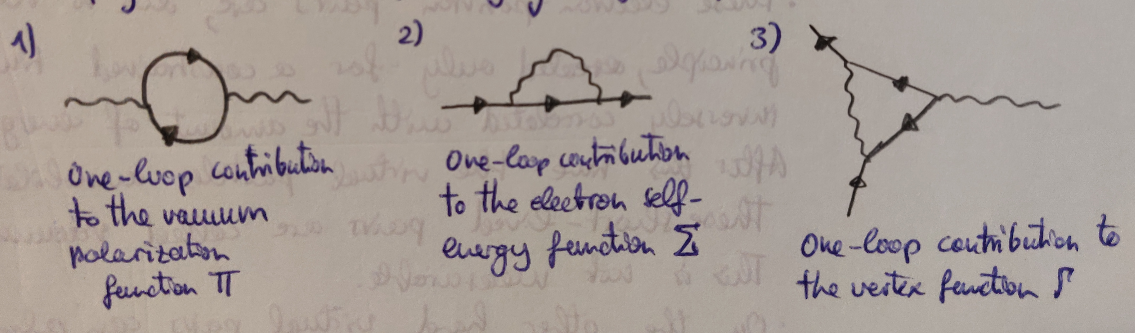
\includegraphics[width=0.7\linewidth]{gfx/DivergingIntegralsQED}
	\caption{\itshape Diverging integrals in QED appearing higher than tree level.}
	\label{fig:divergingintegralsqed}
\end{figure}
A theory is renormalizable, thus meaningful after renormalization, if the number of diverging diagrams is finite. The reason for this is that to get observables renormalized one needs a finite number of constants to maintain the predictive value of the theory untouched.
\subsubsection{Corrections to the fermion propagator}
Taking QED interactions into account the Feynman propagator $S_F(x-y)= \feynmandiagram[horizontal=a to b]{a [particle=y]-- [fermion] b [particle=x] };$ is corrected like
\begin{align}
	\expval{\hat{T}\{\psi(x) \bar{\psi}(y)\}}{\Omega} &=
	\feynmandiagram[horizontal=a to b]{a [particle=y] --c-- [fermion] b[particle=x]}; 
	+ \feynmandiagram[horizontal=a to b]{a [particle=y]--c--[fermion] d--b [particle=x], c--[boson, half left] d };\nonumber \\
	&	+\feynmandiagram[horizontal=a to b]{ a[particle=y] --c--[fermion] d -- e--f--[fermion] g--b[particle=x],
	c--[half left, boson]g, d -- [half left, boson ]f   } ; \\
&= 
\feynmandiagram[horizontal=a to b]{a[particle=y] -- c [blob] -- b [particle=x] };.
\end{align}

\begin{mybox}{Electron self-energy}
	Let 
	\begin{equation}
	\feynmandiagram[horizontal=a to b] {a [particle=A]--c [particle=$\left(1PI\right)$]--b[particle=B]  }; \equiv - i \sum(\slashed{p})_{AB}
	\end{equation}
	denote the amputated $1PI$ diagram. $\sum(\slashed{p})$ \emph{is called self-energy of the electron.}
	$\Rightarrow$ 
	\begin{align}
		\expval{\hat{T}\{\psi(x) \bar{\psi}(y) \}}{\Omega} &= \feynmandiagram[horizontal=a to b]{a[particle=y] --c--[fermion] b[particle=x] };
		+ \feynmandiagram[horizontal=a to b]{a--[fermion] c [particle=$\left(\sum\right)$]--[fermion] b  }; \nonumber \\
		&+ \feynmandiagram[horizontal=a to b]{a --[fermion]c[particle=$\left(\sum\right)$ ]--[fermion] d[particle=$\left(\sum\right)$] --[fermion]b  }; + \dots
	\end{align}
\end{mybox}
Where the full Feynman propagator for interacting QED theory takes the form (via Dyson resummation) 
\begin{equation}
\feynmandiagram[horizontal=a to b]{a [particle=y] --c [blob] -- b[particle=x]  };
= \int \frac{\md^4 p}{(2 \pi)^4} e^{-i p\cdot (x-y)} \; \frac{i}{\gamma \cdot p-m_0 - \sum(\slashed{p})+i \epsilon }.
\end{equation}



\subsubsection{Corrections to the photon propagator}
\begin{mybox}{Photon self-energy}
The Fourier transform of the photon propagator, denoted by $\feynmandiagram[horizontal=a to b]{a --[boson] c [blob] --[boson]b};$, can be derived via Dyson resummation from the $1PI$ diagram 
\begin{equation}
\feynmandiagram[horizontal=a to b]{a[particle=$\mu$] -- [boson] c -- [boson] b[particle=$\nu$] };
\equiv i \Pi^{\mu \nu} (q^2) = 
\end{equation}
which is the \emph{self-energy of the photon or vacuum polarization}.
\end{mybox}
Vacuum polarization describes the process in which a background electromagnetic field produces virtual electron-positron pairs that change the distribution of charges and currents that generated the original electromagnetic field. It is also referred to as the \emph{self-energy of the gauge boson(photon)}.\\
\\
These electron-positron pairs are, due to Heisenberg's uncertainty principle, created only for a constrained time, having duration inversely correlated with the amount of energy of the fluctuation. After this time the virtual particles annihilate each other. These short-lived pairs are called \emph{vacuum bubbles}. This is not measurable.\\
On the other hand virtual pairs can also occur as a photon progress, as seen in \ref{fig:divergingintegralsqed}; the effect on other processes is measurable.\\
$\Rightarrow$ Such charged pairs act as an electric dipole. In the presence of an electric field, e.g. the electromagnetic field around an electron, these particle-antiparticle pairs reposition themselves, thus partially counteracting the field.\\
The field therefore will be weaker than would be expected if the vacuum were completely empty. This reorientation of the short-lived particle-antiparticle pairs is referred to as  \emph{vacuum polarization}.

\subsubsection{Corrections to the interaction vertex}
\begin{mybox}{Vertex function}
	We define an effective vertex by summing up all loop-corrections. This is the \emph{vertex function} $\Gamma$, which describes the coupling between a photon and an electron beyond leading order, it is the one particle irreducible correlation function which involves $ \psi, \bar{\psi}$ and $A_{\mu}$:

\end{mybox}
	
\begin{figure}
	\centering
	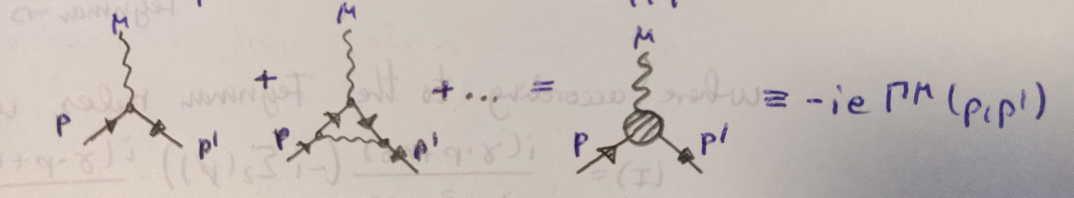
\includegraphics[width=0.7\linewidth]{gfx/VertexFunctionQED}
	\caption{\itshape Definition of the vertex function, summing up all loop corrections.}
	\label{fig:vertexfunctionqed}
\end{figure}
We will compute these corrections to 1-loop order. The diagrams will exhibit:
\begin{enumerate}
	\item Ultraviolet (UV) divergences from integrating the momenta of particles in the loop up to infinity.
	\item Infra-red (IR) divergences if the diagram contains massless particles (i.e. photons) running in the loop
\end{enumerate}
The general status of these divergences is as follows
\begin{enumerate}
	\item UV divergences require regularization of the integral and can be absorbed in a clever definition of the parameters via renormalization.
	\item IR divergences in loop-diagrams cancel if physical observables are computed.
\end{enumerate}



\subsection{Self-energy of the electron at 1-loop}
At 1-loop order the electron propagator takes the form 
\begin{equation}
	 \expval{\hat{T}\{\psi(x) \bar{\psi}(y)\}}{\Omega} =
	 \feynmandiagram[horizontal=a to b]{a [particle=y] -- [fermion] c-- b [particle=y]};
	 + \underbrace{\feynmandiagram[horizontal=a to b]{a[particle=y] --[fermion] c-- b[particle=x]}; }_{\stackrel{Feynman}{\Rightarrow} \int \frac{\md^4 p}{(2 \pi)^4} e^{-i p(x-y) } \cdot (I) }
\end{equation}
where according to the Feynman rules we have
\begin{equation}
	(I) = \frac{i(\gamma \cdot p +m_0)}{p^2-m^2_0+i \epsilon} \left(-i \sum_2(\slashed{p})\right) \frac{i(\gamma \cdot p+m_0)}{p^2-m^2_0 +i\epsilon}.
\end{equation}
$\Rightarrow$ The amputated 1-loop contribution corresponds to omitting the two outer fermion propagators and is thus given by:
\begin{equation}
	-i \sum_2(\slashed{p}) = (-i e)^2 \int \frac{\md^4 k}{(2 \pi)^4} \gamma^{\mu} \frac{i(\slashed{k}+m_0)}{k^2-m^2_0+i \epsilon} \gamma^{\nu} \frac{(-i \eta_{\mu \nu})}{(p-k)^2 + i \epsilon}.
\end{equation}
This integral has a IR-divergence near $k=0$ if $p\rightarrow0$. We will introduce a fictitious small photon mass $\mu$ to regulate the IR divergence:
\begin{equation}
	\Rightarrow i \sum_2(\slashed{p}) = (-ie)^2 \int \frac{\md^4 k}{(2 \pi)^4} \gamma^{\mu} \frac{i (\slashed{k}+m_0)}{k^2-m^2_0 +i \epsilon} \gamma_{\mu} \frac{-i}{(p-k)^2-\mu^2+i \epsilon}.
\end{equation}
The evaluation of such typical momentum integrals proceeds in 3 steps.
\subsubsection{Step 1: Feynman parameters}
The integrand contains a fraction of the form $\frac{1}{AB}$ with $A=(p-k)^2-\mu^2+i \epsilon$ and $B=k^2-m^2_0+i\epsilon$. Any $A,B \in \mathbb{C}\ \{0\}$ satisfies
\begin{equation}
	\frac{1}{AB} = \int_0^1 \md x \quad \frac{1}{\left[xA+(1-x) B\right]^2} 
\end{equation}
with $x:$ Feynman parameter. \\
$\Rightarrow$ in our case applying the identity with some algebra yields
\begin{equation}
	\frac{1}{AB} = \int_0^1  \md x \; \frac{1}{[l^2- \Delta+i \epsilon]^2}, \; l=k-xp,\; \Delta=-x(1-x) p^2+x \mu^2 +(1-x) m^2_0.
\end{equation}
With some more Dirac algebra manipulations we find
\begin{equation}
	-i \sum_2(\slashed{p}) = -e^2 \int_0^1 \md x \int \frac{\md^4 l}{(2 \pi)^4} \; \frac{-2 \slashed{p} +4 m_0}{[l^2-\Delta+i\epsilon]^2}.
\end{equation}

\subsubsection{Step 2: Wick rotation}
The Wick rotation relates typical integrals appearing in loops like $\int \frac{\md^4 l}{(2 \pi)^4} \frac{1}{[l^2-\Delta +i\epsilon]^n}$ to Euclidean integrals.\\
The $^0$ integral is in fact a complex contour integral along the real axis. The value of this integral is unchanged if we deform the contour without hitting any pole. Therefore we can rotate the contour by $90^°$ counter-clockwise to lie along the imaginary axis:
\begin{figure}
	\centering
	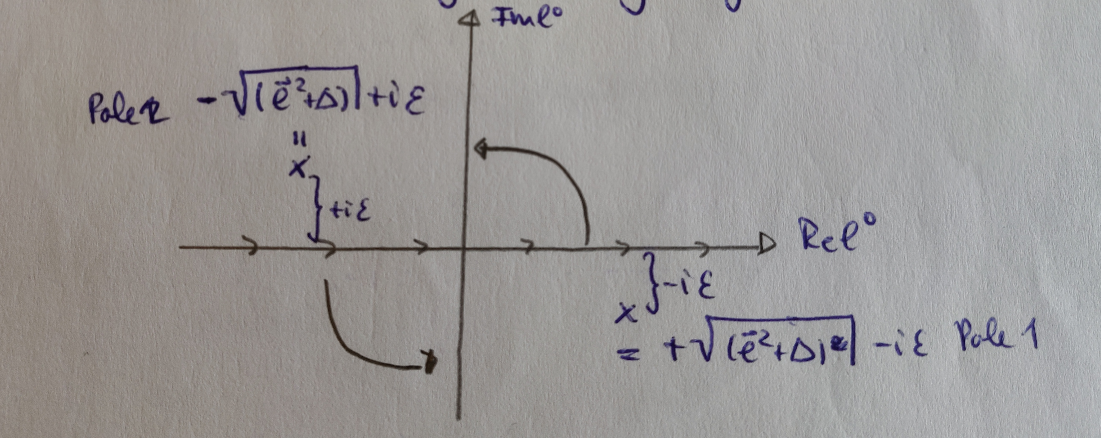
\includegraphics[width=0.7\linewidth]{gfx/Wickrotation}
	\caption{\itshape How to perform integral in the renormalization procedure by a Wick rotation.}
	\label{fig:wickrotation}
\end{figure}
Introducing the Euclidean 4-momentum $l_E = (l^0_E, \vec{l}_E)$ as 
\begin{equation}
	l^0=i l^0_E, \; \vec{l}=\vec{l}_E \; \Rightarrow \; l^2=-l^2_E\equiv \; -i \sum_j (l^j_E)^2
\end{equation}
we can write the integral as
\begin{equation}
	\int \frac{\md^4 l}{(2 \pi)^4} \, \frac{1}{[l^2-\Delta+i\epsilon]^m} = (-1)^m i \int \frac{\md^4 l}{(2 \pi)^4} \, \frac{1}{[l^2_E+\Delta - i \epsilon]^m}.
\end{equation}
Since we won't need the $i\epsilon$ any longer we can omit it at this stage. We can now perform the integral as a spherical integral in $\mR^4$.





























\chapter{Advanced Quantum Field Theory}
\section{Bosonic (scalar) field theory in pathintegral language}
\subsection{??Coherent states in QFT}
\begin{mybox}{}
	In terms of field operators $\phi(x)$
	\begin{equation}
		\ket{\varphi(x)}:= e^{\varphi\cdot \phi} \ket{\Omega} \; \text{with} \; \varphi\cdot\phi\equiv\int\md^d x \varphi(x) \phi(x)
	\end{equation}
	the expectation value of $\phi(x)$ in a system in a coherent state is the classical field
	\begin{equation}
	\bra{\varphi(x)}\phi(x) \ket{\varphi(x)} = \varphi(x).
	\end{equation}
\end{mybox}
















\subsection{Path integral in Quantum Mechanics}
The path integral provides a formulation of quantum theory completely equivalent to the canonical quantization.\\
\\
A quantum mechanical transition amplitude $\braket{q_f,t_f}{q_i,t_i} = \bra{q_f} e^{i \hat{H}(t_f-t_i)} \ket{q_i}$ can, by partitioning of the \emph{transition time} $\delta t=\frac{t_f-t_i}{N+1}$ and insertion of \emph{complete sets of states} $\mathcal{I}= \int_{\mR} \md q_k \, \ket{q_k}\bra{q_k}$ between each partition, be expressed as 
\begin{equation}
	\braket{q_f,t_f}{q_i,t_i} = \lim_{N\rightarrow\infty} \int \frac{\md p_0}{2 \pi} \prod_{k=1}^{N} \frac{\md p_k \md q_k}{2 \pi} \exp\left[i \sum_{k=0}^{N} \left(p_k \frac{q_{k+1}-q_k}{\delta t} - H\right) \delta t\right]
\end{equation}
\marginpar{Thus, we have boundary conditions for $q(t)$, whereas $p(t)$ is free at the endpoints.}
which is per definition equivalent to
\begin{equation}
	\braket{q_f,t_f}{q_i,t_i} = \int_{q(t_i)=q_i}^{q(t_f)=q_f}  \mathcal{D}q(t) \mathcal{D}p(t) \, \exp\left[i\int_{t_i}^{t_f} \md t \left(p \dot{q} - H(p,q) \right)\right]
\end{equation}
with 
\begin{equation}
	S[p,q] \equiv \int_{t_i}^{t_f} \md t \; L(p,q) \quad \mathrm{and} \quad L(p,q) \equiv p \dot{q} - H(p,q)
\end{equation}
which holds true for every Weyl-ordered Hamiltonian, e.g. $H=f(p)+V(q)$.\\
\begin{mybox}{Feynman path integral}
	\emph{Analytic continuation} by rotating $t$ onto the lower half-plane via $\delta t \rightarrow \delta t (1-i \epsilon)$ followed by performing the momentum path integral as a Gaussian yields the Feynman-Kac formula
	\begin{align}
		\braket{q_f,t_f}{q_i,t_i} &= \lim_{N\rightarrow\infty} C^{N+1} \prod_{k=1}^{N} \int \md q_k \, e^{i \int_{t_i}^{t_f} \md t \, L(q,\dot{q})}\\
		&= \int_{q(t_i)=q_i}^{q(t_f)=q_f} \mathcal{D}q(t) e^{i \int_{t_i}^{t_f} \md t\, L(q,\dot{q})}\nonumber
	\end{align}
	where the factor $C^{N+1} = \left(\frac{-i m}{2 \pi \delta t}\right)^{\frac{N+1}{2}}$ is absorbed into $\mathcal{D}q(t)$, using $C:= \sqrt{\frac{-im}{2 \pi \delta t}}$.s
\end{mybox}
This is interpreted as:\\
The transition amplitude $\braket{q_f,t_f}{q_i,t_i}$ counts all possible continuous path from $q_i$ to $q_f$ weighted by $\exp\left[\frac{i}{\hbar} S\right]$. In the \emph{classical limit} $S[q,\dot{q}] \gg \hbar$ and due to the strongly oscillating phase of the integrand, the right-hand side is dominated by paths for which the action becomes \emph{stationary}
\begin{equation}
	\frac{\delta S}{\delta q} =0 \quad \Leftrightarrow \; \mathrm{principle\,of\,least\, action}.
\end{equation}
This is the \emph{classical path}, quantum physics is obtained by summing up all additionally possible paths with the classical path via the path integral.\\
\\
The limit $N\rightarrow\infty$ and the ensuing interpretation of the path integral as an integral over all continuous paths from $q_i$ to $q_f$ can be made mathematically rigorous - at least for $H=\frac{p^2}{2m} +V(q)$ -by passing to the Euclidean theory.
\subsubsection{Wick rotation - TO DO}
The path integral itself is ill-defined. We use Wick rotation $t=-i \tau$, $\tau \in \mR_{>0}$ with $\tau$ being called \emph{Euclidean time}, such that 
\begin{equation*}
	\md s^2 = \md t^2 - \md \vec{x}^2 = - (\md \tau^2 + \md \vec{x}^2)
\end{equation*}
as if we were working in a spacetime of Euclidean signature. Then we also go over to the Euclidean action
\begin{equation*}
	iS=- \int \md \tau \left[\half \underbrace{\left(\frac{\md q}{\md \tau}\right)^2}_{>0} +V(q)\right] \equiv - S_E
\end{equation*}
such that if $V(q)$ is positive, then $S_E>0$.\\
Then, in Euclidean description we find
\begin{equation*}
	Z[J] = n \int \mD q \exp \left[-S_E - \int \md \tau J(\tau) q(\tau)\right]
\end{equation*}
such that the integral is now more convergent than before, the Wick rotation makes it easier. The path integral is only well-defined in Euclidean signature. Wick rotation then also guarantees (compare \ref{eq:relationfreeInteractingvacuum}) that it is only the vacuum $\ket{0}$ which enters into correlations functions.
\subsubsection{Why do I need the PI ?}
\begin{enumerate}
	\item All the (Lorentz) symmetries are manifest in the PI calculation. Manifest hear means that everything will be Lorentz invariant all the time. In canonical quantization on the other hand, you quantize time slices by defining ladder operators via \emph{equal time} commutation relations, which means that we lose Lorentz invariance on the way, but then the whole evolution, tracking all the time slices, is Lorentz invariant in total.
	\item PI are forgiving, in the sense that you can be cavallier about the structure of the Hilbert space. Especially gauge theories have a tricky Hilbert space, which becomes easier in PI language. E.g. QED in Hamiltonian (canonical) quantization, the photon has $2$ polarizations but $A_\mu$ has $4$. $2$ dof. have to be dropped (via gauge fixing), Hilbert space is done via Gupta-Bleuler quantization or Dirac brackets. The redundant terms have to be get rid off. Even more difficult for non-abelian gauge theories.
\end{enumerate}


 

\subsection{The path integral for scalar fields}
\begin{mybox}{Path integral of a real scalar field}
	The pathintegral is understood as the transition amplitude of coherent states, which for real scalar fields $\phi(x)$ (as opposed to particles) is given by
\begin{align}
	\braket{\phi_f(\vec{x} ),t_f }{\phi_i(\vec{x}),t_i} &= \int \mathcal{D}\phi(x) \mathcal{D}\pi(x) \\
	&\quad e^{i \int_{t_i}^{t_f} \md \int \md^4 x [\phi \dot{\phi}-\mH(\pi,\phi)]} |^{\phi(\vec{x},t_i)=\phi_i(\vec{x})}_{\phi(\vec{x},t_f)=\phi_f(\vec{x})}\nonumber \\
	&= \int_{\phi(\vec{x},t_i) = \phi_i(\vec{x})}^{\phi(\vec{x},t_f)=\phi_f(\vec{x})} \mathcal{D}\phi(x) e^{i \int_{t_i}^{t_f} \md t \int_{\mR^3} \md^3 x \mL[\phi(x)]},
\end{align}
where the latter equality holds for $\mH(\pi,\phi)=\frac{\pi^2}{2}+V(\phi)$.
\end{mybox}
Note the identical spatial coordinates of $\phi_f(\vec{x}$ and $\phi_i(\vec{x})$.
\subsection{A more closer look in terms of propagators}
Consider a real scalar field $\phi(x)=\phi(\vec{x},t)$
\begin{equation}
	S[\phi] = \half \int \md^4 x \left[(\partial \phi)^2-m^2\phi^2\right] \stackrel{PI}{=} \half \int \md^4 x \phi(x) \left[-\partial^2-m^2\right] \phi(x)
\end{equation}
such that the classical e.o.m. is instantly provided with $(\partial^2+m^2)\phi(x) =0$. Now we quantize the PI over fields $\phi(x)$.\\
Calculate the two-point correlator with
\begin{align*}
	\bra{0} \mathcal{T} \phi(x) \phi(y) \ket{0} &= D_F(x-y) =Z^{-1}_0 \int \mD \phi \phi(x) \phi(y) \exp\left[i S[\phi]\right] \\
	&= \frac{1}{Z_0} \left[-i \frac{\delta}{\delta J(x)}\right]\left[-i \frac{\delta}{\delta J(y)}\right] Z[J] |_{J=0}
\end{align*}
where the order of the derivatives does not matter since the correlator is time-ordered. For this calculation, we need to find an expression for $Z[J]$ and take the derivatives. Note however, that the generating function has the shape of a Gaussian.\\
\begin{mybox}{Reminder for Gaussian integration}
	\begin{align}
	&\int \md x_1 \dots \md x_N \exp\left[-\half x^a A_{ab} x^b + i J_a x^a\right] \\
	&= \sqrt{\frac{(2 \pi)^N}{\det A}} \exp \left[- \half J_a \left(A^{-1}\right)^{ab} J_b\right]\nonumber
	\end{align}
	with $N\in [0,\infty]$.
\end{mybox}
Identify the operator from the action:
\begin{equation*}
	A = i (\partial^2+m^2)
\end{equation*}
such that, using $\det\left(\frac{A}{2 \pi}\right)= \frac{\det A}{(2 \pi)^N}$ for $A\in M^{N\times N}$
\begin{equation*}
	Z[J]=\left[\det\left(\frac{\partial^2+m^2}{-2\pi i}\right)\right]^{-\half} \exp \left[-\half \int \md^4x\md^4y J(x) D_F(x,y) J(y)\right]
\end{equation*}
where $A^{-1} \equiv D_F$ the Feynman propagator
\begin{equation*}
	i(\partial^2+m^2) D_F(x,y) = \delta^{(4)}(x-y).
\end{equation*}
Note that this determinant is a functional determinant which acts on an operator, which itself is acting on the space of functions. How do you compute this determinant ? Figure out the eigenvalues of the operator and then the determinant is just given by the product of all these eigenvalues (usually infinite product). One possible eigenbasis of the operator $(\partial^2+m^2)$ are the plane wave $e^{ip(x-y)}$ or gaussians.\\
Thus, from $Z[J]$ we take functional derivatives and find (implied by the notation)
\begin{equation*}
\Rightarrow\quad \bra{0} \mathcal{T}\phi(x) \phi(y) \ket{0} = D_F(x,y).
\end{equation*}









\subsection{Vacuum correlation functions}
\begin{mybox}{N-point correlators}
	For n-point correlation functions we find in the interacting theory, that the time ordering appears automatically, which means that under the path-integral the operators are merely $\mathbb{C}$-numbers, such that ordering is not necessary anymore:
	\begin{align}
	&\frac{\bra{\Omega;out} \mathcal{T}\prod_i \phi^{(H)}(x_i) \ket{\Omega;in}}{\braket{\Omega;out}{\Omega;in}} \\
	&= \lim_{T\rightarrow \infty(1-i \epsilon)} 
	\frac{\int \mathcal{D}q(x) \mathcal{D}\pi(x)\prod_i \phi(x_i) e^{-i \int_{-T}^{T} \md t \int \md^dx[\pi \dot{\phi}-\mH(\pi,\phi)]} }{\int \mathcal{D}q(x) \mathcal{D}\pi(x) e^{i \int_{-T}^T \md t \int \md^dx[\pi \dot{\phi}-\mH(\pi,\phi)] }}\nonumber.
	\end{align}
such that we have for $\mH(\pi,\phi)=\frac{\pi^2}{2}+V(\phi)$
\begin{equation}
	\bra{ \Omega}\mathcal{T}\phi^{(H)}(x) \phi^{(H)}(y) \ket{\Omega}\propto \int \mathcal{D}\phi \phi(x) \phi(y) e^{i S[\phi]}.
\end{equation}
\end{mybox}
This holds for general operators, such that
\begin{equation}
	\int \mathcal{D}\phi F[\phi] e^{iS[\phi]} = \bra{ \Omega}F[\hat{ \phi}]\ket{\Omega}.
\end{equation}
\begin{mybox}{Master formula for cumulants}
	The master formula for an n-point quantum correlation function reads
	\begin{align}
		G(x_1,\dots,x_n) &= \expval{\hat{T} \prod_{j=1}^{n} \hat{\phi}_H(x_j) }{\Omega} \nonumber\\
		&= \lim_{T\rightarrow\infty(1-i\epsilon)} \frac{\int \mathcal{D}\phi(x) \prod_{j=1}^{n} \phi(x_j) e^{-i \int_{-T}^T \md^4 x \mL(\phi)(x) } }{\int \mathcal{D}\phi(x) e^{i \int_{-T}^T \md^4 x \mL [\phi(x)]}}.
	\end{align}
\end{mybox}
In a perturbatively renormalizabe theory, the action can be renormalized order by order such that the perturbatively expanded correlation functions are finite in the continuum limit, order by order. One can evaluate the path-integral in an exact, non-perturbative manner by e.g. \emph{Lattice Field Theory} (c.f. page 181).

\subsection{Operator equations in pathintegral formalism}
\begin{mybox}{}
	An operator equation is a pathintegral equation that holds under arbitrary insertions, i.e.
	\begin{equation}
		\hat{ \mO}_1 = \hat{\mO}_2 \Leftrightarrow \int \mathcal{D}\phi \mO \mO_1 e^{iS[\phi]} = \int \mathcal{D}\phi \mO \mO_2 e^{iS[\phi]} \; \text{for all} \; \mO.
	\end{equation}
\end{mybox}





\subsection{Generating Functional for Correlation Functions, partition function and $N$-point correlator}
\begin{mybox}{Generating functional}
	The generating functional $Z[J]$ of Green's functions $G(x_1, \dots, x_n)$ for some source $J(x)$ reads
	\begin{equation}
	Z[J] = \int \mathcal{D}\phi \; e^{i S[\phi] + i J \cdot \phi },
	\end{equation}
	where the functional inner product is defined as
	\begin{equation}
	J \cdot \phi = \int_{\mR^{3,1}} \md^4 x J(x)\phi(x).
	\end{equation}
\end{mybox}
$Z[J]$ maps the function $\phi(x)$ to a number in $\mathbb{C}$. It is called generating functional because
\begin{equation}
\frac{Z[J]}{Z[0]} = \sum_{n=0}^{\infty} \frac{i^n}{n!} \left(\prod_{j=1}^{n} \int_{\mR^{3,1}} \md^4 x_j \, J(x_j) \right)G(x_1,\dots,x_n).
\end{equation}

\begin{mybox}{Calculating cumulants from the generating functional}
	This can be solved for $G(x_1,\dots,x_n)$ using the tools of functional calculus:
	\begin{equation}
	G(x_1,\dots,x_n) = \frac{1}{Z[0]} \left[\prod_{j=1}^{n} \frac{\delta}{i \delta J(x_j)}\right] Z[J] |_{J=0},
	\end{equation}
	with the functional derivative
	\begin{equation}
	\frac{\delta \phi(y) }{\delta \phi(x)} = \delta_D(x-y).
	\end{equation}
\end{mybox}
\begin{mybox}{Partition function}
	The partition function is the vacuum-vacuum amplitude
	\begin{equation}
		Z[0] = \int \mathcal{D}\phi e^{i S[\phi]} = \bra{ \Omega;out}\ket{\Omega;in}.
	\end{equation}
	The generating functional is the vacuum-vacuum amplitude in presence of an external classical current $J(x)$ when normalization is chosen such that $Z[0]=\braket{\Omega}{\Omega}=1$
	\begin{equation}
		Z[J]= \int \mathcal{D}\phi e^{i S[\phi] + i \int \md^4 x \phi(x) J(x)} \equiv \int \mathcal{D}\phi e^{iS[\phi]} e^{i J\cdot \phi} = \braket{ \Omega;out}{\Omega;in}_J.
	\end{equation}
	The generating expansion
	\begin{equation}
	\frac{Z[J]}{Z[0]} = \int_{n=1}^{\infty} \int \md x_1 \dots \int \md x_n J(x_1) \dots J(x_n) G(x_1,\dots,x_n) 
	\end{equation}
	can be used to find the $N$-point correlator
	\begin{align}
		G(x_1,\dots,x_n) &\equiv \bra{ \Omega}\mathcal{T}\phi(x_1)\dots \phi(x_n)\ket{\Omega} \\
		&= \frac{1}{Z[J]} \left(\frac{1}{i} \frac{\delta}{\delta J(x_1)}\right)\dots \left(\frac{1}{i} \frac{\delta}{\delta J(x_n)}\right) Z[J] |_{J=0} \nonumber \\
		&=: \frac{Z^{(n)}[0]}{Z[0]}\nonumber
	\end{align}
which are in-out correlators, but the notation is dropped for the vacuum.
	
\end{mybox}
$Z[0]$ contains no external points and represents the partition function $Z[0]=e^{\sum_i V_i}$, where the sum runs over all vacuum bubbles $V_i$ of the theory. Consequently, $\frac{Z[J]}{Z[0]}$ contains no vacuum bubbles.\\
\\
We can pull the derivatives over the normalization $\frac{1}{Z[J]}$ and compensate by adding the one-point function $\expval{\phi}_J = \frac{1}{Z[J]}\frac{\delta}{i\delta J} Z[J]$ to get
\begin{equation}
\label{eq:cumulantsExpression}
	G(x_1,\dots,x_n) = \prod_{j=1}^{n} \left(\frac{1}{i} \frac{\delta}{\delta J(x_j)} + \expval{\phi(x_j)}_J\right) |_{J=0}.
\end{equation}


\subsection{Free scalar theory}
\begin{mybox}{}
\begin{equation}
	S_0[\phi] = - \half \int \md^4 x \phi(x) (\partial_\mu \partial^\mu+m^2_0)\phi(x)
\end{equation}
with the notation
\begin{equation*}
	S_0[\phi] = -\half \phi \cdot K\phi \; \text{with } K:= \delta(x-y) (\partial^2_x+m^2_0).
\end{equation*}
For $(\partial^2+m^2)D_F(x)=-i \delta(x)$ the sign convention $K$ is related to the propagator as
\begin{equation}
\label{eq:propagatorInverted}
	K^{-1}(x,z)=iD_F(x-z)
\end{equation}
such that we can write
\begin{equation}
	S_0[\phi] = \half \phi\cdot iD_F\cdot \phi
\end{equation}
or ’completing the square’
\begin{equation}
	Z_0[J] = \int \mathcal{D}\phi e^{- \half \phi \cdot D^{-1}_F\cdot \phi + i\phi \cdot J} = \int \mathcal{D}\phi e^{\frac{i}{2} \phi \cdot K \cdot \phi-\half J\cdot D_F \cdot J} = Z_0[0] e^{\frac{i}{2} J\cdot D_F i\cdot J}.
\end{equation}

\end{mybox}
$Z_0[0]$ is a functional Gaussian integral and a functional determinant since
\begin{equation}
	Z_0[0] = \int \mathcal{D}\phi e^{-\half \phi\cdot D^{-1}_F\cdot \phi} = \sqrt{\frac{(2 \pi)^\infty}{\det D^{-1}_F}} = \sqrt{\frac{(2 \pi)^\infty}{\det -iK}}
\end{equation}
Proof of \ref{eq:propagatorInverted}:\\
With the definition of the inverse of the inverse of a kernel
\begin{equation*}
	KK^{-1} = \mI \; \Leftrightarrow \; \int \md z K(x,z) K^{-1}(z,y) = \delta(x-y),
\end{equation*}
we can identify the defining equation of the propagator $(\partial^2+m^2)D_F(x) = -i \delta(x)$ in
\begin{align*}
	\int \md z \delta(x-z) (\partial^2_x+m^2) K^{-1}(z,y) &= (\partial^2_x +m^2) K^{-1}(x,y) = \delta(x-y) \\
	&\Leftrightarrow\; K^{-1}(x,y) = i D_F(x-y) \quad \blacksquare
\end{align*}













\subsection{Perturbative Expansion in Interacting Theory}
$Z_0[0]$ is in general a divergent quantity, but i can be rigorously defined by a regularization procedure.\\
All physical quantities are computed in the regularized theory and the expression $Z_0[0]$ cancels in all such expressions because the correlation functions derive from $\frac{Z[J]}{Z[0]}$.\\
To compute a $2n$-point function one expands the exponential precisely to $n$-th order, while the $2n+1$-functions vanish.\\
\\
Consider an action with an interaction
\begin{align}
	S[\phi] &= S_0 [\phi] \quad + \int_{\mR^{3,1}} \md^4 x \, \mL_{int} [\phi] \\
	\Rightarrow Z[J] &= \exp\left[i \int_{\mR^{3,1}} \md^4 x \, \mL_{int} \left[- \frac{i \delta}{\delta J} \right]   \right] Z_0[J].
\end{align}
\begin{mybox}{Perturtbation theory, Feynman rules etc.}
	\begin{subequations}
		\begin{align}
				Z[J] &= e^{i \int \md^4 x \mL_{int} (\frac{\delta}{i \delta J} ) } Z_0[J] \\
				&= Z_0[0] e^{i \int \md^4 x \mL_{int} (\frac{\delta}{i\delta J} ) } e^{\half i J\cdot D_F \cdot i J},\nonumber \\
						Z[J] &= Z_0[0] e^{\half \frac{\delta}{\delta \phi} \cdot D_F \cdot \frac{\delta}{\delta \phi}} e^{i \int \md^4 x \mL_{int} (\phi)+ i J\cdot \phi} |_{\phi=0},\\
						\expval{F[\phi]}_0 &:= e^{\half \frac{\delta}{\delta \phi} \cdot D_F \cdot \frac{\delta}{\delta \phi}} F[\phi] |_{\phi=0},\label{eq:wickPIexpval}\\
						Z[J] &= Z_0[0] \expval{e^{i \int \md^4 x \mL_{int}(\phi) + i J\cdot \phi}}_0,\\
						\expval{\phi(x_1)\cdot \phi(x_n)}_0 &= \expval{\mathcal{T}\{\phi^{(I)}(x_1)\cdot \phi^{(I)}(x_n)  \}}{0},\\
						\frac{Z[J]}{Z[0]} &= \frac{\expval{e^{i \int \md^4 x \mL_{int} (\phi) + i J\cdot \phi}_0}}{\expval{e^{i \int \md^4 x \mL_{int } (\phi)}}_0},\\
						G(x_1,\dots,x_n) &= \frac{\expval{\phi(x_1)\dots \phi(x_n) e^{i \int \md^4 x \mL_{int} (\phi)}}_0}{\expval{e^{i \int \md^4 x \mL_{int}(\phi)}}_0}\label{eq:cumulantsPI}.
		\end{align}
	\end{subequations}
\end{mybox}
A useful identity for functionals $F,G$ and a scalar field $\phi$ is
\begin{equation}
	F[\frac{\delta}{i \delta J}]G[iJ] e^{i J\cdot \phi} = G[\frac{\delta}{\delta \phi}] F[\phi] e^{i J\cdot \phi}.
\end{equation}












\subsection{Wick's theorem for bosons revisited}
\begin{mybox}{Wick theorem in path integral language}
	We can recover the Feynman rules and Wick's theorem equivalently as in the canonical quantization with the definition for function $F[\phi]\rightarrow \expval{F[\phi]}_0$ as above with the scalar Feynman propagator $D_F$.\\
	In pathintegral formalism Wick's theorem arises simply from applying the product rule of functional derivatives to the expansion of \ref{eq:wickPIexpval}, e.g. for $n=2$
	\begin{equation}
		\expval{\phi(x) \phi(y)}_0 = e^{\half \frac{\delta}{\delta \phi} \cdot D_F\cdot \frac{\delta}{\delta \phi} } \phi(x) \phi(y) |_{\phi=0} = \left[\half \frac{\delta}{\delta \phi} \cdot D_F \cdot \frac{\delta}{\delta \phi}\right] \phi(x) \phi(y),
	\end{equation}
	where terms of order $2k<n$ cancel at $\phi=0$ and terms of order $2k>n$ vanish since they have more derivatives than fields, such that only the term $2k=n$ term contributes.\\
	We can identify :
	\begin{equation}
		\langle \phi(x_1) \phi(x_2) \rangle_0 = \expval{\hat{T} \hat{\phi}(x_1) \hat{\phi}(x_2)}{0} = \contraction{}{\phi(x_1)}{}{\phi(x_2)} \phi(x_1) \phi(x_2),
	\end{equation}
	which gives us the results of Wick's theorem
	\begin{align}
		\langle \phi_1 \dots \phi_{2n} \rangle_0 = \contraction{}{\phi_1}{}{\phi_2} \phi_1 \phi_2 \contraction{}{\phi_3}{}{\phi_4} \phi_3 \phi_4 \dots \contraction{}{\phi_{2n-1}}{}{\phi_{2n}}  \phi_{2n-1} \phi_{2n}  \\
		&+ \text{all other contractions}.\nonumber \\
		\langle \phi_1 \dots \phi_{2n+1} \rangle_0 &=0.
	\end{align}
\end{mybox}
Note that the $N$-point function being a product of $2$-point function can be seen from the fact that $e^{iS[\phi]}$ is a Gaussian, i.e. it only depends on $2$-point correlators.
\subsubsection{Recovering Feynman rules}
With Wick's theorem at hand we recover the exact same Feynman rules as in operator language from the Gell-Mann-Low formula in the interaction picture for position and momentum space.\\
Note, that $\phi(x_i)$ or $\frac{\delta}{i \delta J(x_i)}$ corresponds to an external point in the Feynman diagram, that a line between $x_i$ and $x_j$ denotes as always a factor $D_F(x_i-x_j)$ :
\begin{equation}
	\feynmandiagram[horizontal=a to b] {a[particle=$x_i$] --c -- [fermion] d[edge label=$D_F(x_i-x_j)$]-- b[particle=$x_j$]};
\end{equation}
and that interactions only occur if there is a dot on crossing lines:
\begin{equation}
	\feynmandiagram[horizontal=a to b]{a[particle=$x_1$]  -- m --[fermion]z [dot] --n-- [anti fermion] b [particle=$x_2$],
	c [particle=$x_3$] -- [fermion] z , d [particle=$x_4$]--[fermion] z   };
\end{equation}
\subsubsection{Perturbative treatment in Path integral language}
In general, we can decompose the partition function according to
\begin{align}
	Z[J]&= \exp\left[i \int \md^4 x \mL_{int}\left(-\frac{i \delta}{\delta J(x)}\right)\right] \underbrace{\int \mD \phi \exp\left[i S_0 [\phi] + i \int \md^4 y J(y) \phi(y)\right]}_{=Z_0[J]}\nonumber\\
	& Z_0[0] \exp \left[i \int \md^4 x \mL_{int} \left(-\frac{i \delta}{ \delta J(x)}\right)\right] \exp \left[-\half \int \md^4 x \md^4 y J(x) D_F(x,y) J(y)\right]
\end{align}
such that a perturbative expansion can be achieved in terms of expanding the former exponential in orders of the perturbative parameter.

\subsubsection{On the counting of loops}
A fully connected Feynman diagram in momentum space with $E$ external and $I$ internal lines, $V$ vertices, and $L$ loops (number of unfixed momentum integrals) satisfies \emph{Euler's formula}
\begin{equation}
	L = I-V+1 \; \leftrightarrow \; \feynmandiagram[horizontal=a to b] {a[particle=$x_i$] -- c [dot] --[half left] d [dot] -- b [particle=$x_j$] , d--[half left] c  };				\Leftrightarrow1= 2-2+1
\end{equation}
$\Rightarrow$ For $\mL_{int}(\phi) = \frac{\lambda^n}{n!} \phi^n(x)$ we have
\begin{equation}
	E + 2 I \quad = \quad nV,
\end{equation}
because every vertex connects to $n$ lines, while every external line connects to one and every internal line to two vertices. Together with Euler's formula we have
\begin{equation}
	(n-2)V \quad = 2L + (E-2).
\end{equation}
Hence for fixed $E$, an expansion in $L$ corresponds to an expansion in $V$.

\subsection{Cancellation of vacuum bubbles revisited}
\begin{mybox}{}
	In pathintegral formalism, vacuum bubbles of free perturbation theory are cancelled by
	\begin{equation}
		Z[0] = \braket{\Omega;out}{\Omega;in} = (\text{sum of all vacuum diagrams})
			\end{equation}
			order by order of the asymptotic series of the numerator and denominator of \ref{eq:cumulantsPI}, i.e.
			\begin{align}
				\frac{Z^{(n)}[0]}{Z[0]} &= \frac{\expval{\phi(x_1) \dots \phi(x_n) e^{i \int \md^4 x \mL_{int}(\phi)} }_0}{\expval{e^{i \int \md^4 x \mL_{int}(\phi)} }_0} \propto \frac{1+\lambda a}{1+\lambda b}\nonumber \\
				&\propto (1+\lambda a) (1-\lambda b) \propto 1 + \lambda (a-b) + \mO(\lambda^2),
			\end{align}
		where the terms $a$ and $b$ both contain vacuum bubbles but $(a-b)$ does not.
\end{mybox}


\subsection{Scalar Schwinger-Dyson equations of the generating functional}
\subsubsection{Schwinger-Dyson equation}
\begin{mybox}{Symmetries in path integral language}
	An advantage of the path-integral method is that symmetries are more transparent. It becomes clear that classical symmetries carry over to the quantum theory -  but only provided the path integral measure $\mathcal{D}\phi =\mathcal{D}\phi'$ is invariant under a given transformation corresponding to the symmetry. In that case, the Schwinger-Dyson equation
	\begin{align}
		\label{eq:schwingerdyson}
		\left(\frac{\delta S}{\delta \phi} |_{\phi=\frac{\delta}{i \delta J}} + J\right) Z[J] &= 0\\
		\expval{F[\phi]}_J=\expval{F\left[\frac{\delta}{i\delta J}\right]}_J \; \Rightarrow \quad &= \int \mathcal{D}\phi \left[\frac{\delta S}{\delta \phi(x)} + J(x) \right] e^{i\left(S[\phi] + J \cdot \phi \right)}
	\end{align}
states that the classical equation of motion (in presence of a source $J$)
\begin{equation}
	0 = \frac{\delta S}{\delta \phi} + J
\end{equation}
holds as an operator equation in the quantum theory, i.e. it holds inside the path integral. They provide the e.o.m. for Green's functions/for given n-point correlators. Note that these equations of motion are therefore preserved under the transformation $\phi \rightarrow\phi'$.\\
Taking $J=0$ gives the contact terms
\begin{align}
	\label{eq:contacttermsSchwingerdyson}
	&\expval{\mathcal{T}\left[\frac{\delta S}{\delta \phi(x)} \phi(x_1) \dots \phi(x_n)\right]}{\Omega} = \\
	&i\sum_{j=1}^{n} \delta(x-x_j) \expval{\mathcal{T}\left[\phi(x_1)\dots \phi(x_{j-1}) \phi(x_{j+1}) \dots \phi(x_n)\right]}{\Omega} \nonumber
\end{align}
In this form the Schwinger-Dyson equation shows that the equations of motion hold inside a correlation function up to contact terms on the right-hand side
\end{mybox}
Note that this is only true as long as there are no contact terms $\propto \delta_D(x-x_j)$.\\
$\Rightarrow$ The idea is that the interactions of a theory are also represented in its Green's functions. The full Green's functions containing the interaction should also contain the free Green's functions in the \emph{limit of the free theory.}\\
The full 1-point function can be understood in terms of full higher n-point functions and bare interactions as encoded in $S[\phi]$.\\
\\
General Schwinger-Dyson equations can be derived from the fact that
\begin{equation}
	\int \mD \phi \frac{\delta}{\delta \phi} F[\phi] =0
\end{equation}
in analogy to functions sufficiently decaying to infinity
\begin{equation}
	\int_{-\infty}^{\infty} \md x \frac{\md}{\md x}f(x) =0.
\end{equation}
The Schwinger-Dyson equation \ref{eq:schwingerdyson} follows from
\begin{equation}
F[\phi] = e^{i S[\phi] +iJ\cdot \phi}.
\end{equation}
Specifying different functionals $F[\phi]$, e.g.
\begin{equation}
	F[\phi] = e^{i S[\phi]} \phi(x_1) \dots \phi(x_n)
\end{equation}
gives for $n=0,1,\dots$ the result that some classical equations hold (up to contact terms) under the pathintegral or rather as expectation values
\begin{align}
	\expval{\frac{\delta S}{\delta \phi}} &= 0\\
	\expval{\frac{\delta S}{\delta \phi(x)} \phi(x_1)} &= i \expval{\delta(x-x_1)} \\
	&\vdots
\end{align}
General symmetry relations such as Ward-Takahashi identities can be derived from
\begin{equation}
	F[\phi] = \Psi[\phi] e^{i S[\phi] + i J\cdot \phi},
\end{equation}
where 
\begin{equation}
	S[\phi] = S[f[\phi]] \propto S[\phi] + \epsilon \Psi[\phi] \frac{\delta S}{\delta \phi} + \mO(\epsilon^2)
\end{equation}
which leads to general Ward identities (Slavnov-Taylor identity).\\
Proof of \ref{eq:schwingerdyson}:
\begin{align*}
	0&= \int \mD \phi \frac{\delta}{\delta \phi} e^{i S[\phi] + i J\cdot \phi} \\
	&= \int \mD \phi \left(i\frac{\delta S}{\delta \phi} + i J\right) e^{i S[\phi]+ i J\cdot \phi} \quad \blacksquare.
\end{align*}
Proof of \ref{eq:contacttermsSchwingerdyson}, for $n=1$ we have
\begin{align*}
	0&= \int \mD \phi \frac{\delta }{\delta \phi(x)} \left(e^{i S[\phi]} \phi(x_1)\right)\\
	&= \int \mD \phi \left(i \frac{\delta S}{\delta \phi(x)} \phi(x_1)+ \frac{\delta \phi(x)}{\delta \phi(x_1)}\right)e^{i S[\phi]}\\
	&= \int \mD \phi \left(i \frac{\delta S}{\delta \phi(x)} \phi(x_1)+ \delta(x-x_1)\right)e^{i S[\phi]}\quad \blacksquare
\end{align*}









\subsubsection{Quantum Symmetry and scalar Ward-Takahashi identity}
\begin{mybox}{}
	As described above, a quantum symmetry
	\begin{equation}
		\Gamma[\Psi[\phi]] = \Gamma[\phi] 
	\end{equation}
	leaves the action invariant
	\begin{align}
		S[\Psi[\phi]] &= S[\phi] \\
		\text{i.e. } \quad \phi(x) &\rightarrow \phi(x)+\epsilon \delta \phi(x) \text{ such that } S[\phi]  \rightarrow S[\phi]
	\end{align}
and the \emph{pathintegral measure} invariant
\begin{equation}
	\phi(x) \rightarrow \phi(x) + \epsilon(x) \delta \phi(x) \text{  such that } \mD\phi \rightarrow \mD \phi
\end{equation}
\end{mybox}
\begin{mybox}{Ward-Takahashi identity}
For a continuous global classical symmetry $\phi \rightarrow \phi' = \phi + \delta \phi$ with conserved Noether current $j^{\mu} (x)$ given by $\frac{\delta S}{\delta \phi(x)}
\delta \phi(x) = - \partial_{\mu} j^{\mu} (x) =0$ \emph{on-shell} we can find the \emph{Ward-Takahashi identity}
\begin{align}
	&\partial_{\mu} \expval{\hat{T} j^{\mu} \prod_{i=1}^{n} \phi(x_i) }{\Omega} = \\
	&\hspace{-0.6cm}-i \sum_{i=1}^{n} \expval{\hat{T} \phi(x_1) \dots \phi(x_{i-1} \delta \phi(x) \delta^{(4)}_D(x-x_i) \phi(x_{i+1}) \dots \phi(x_n) }{\Omega}
\end{align}
which is derived from the Schwinger-Dyson equation, i.e. the statement of current conservation up to contact terms inside correlation functions.
It equivalently reads
\begin{equation}
	\label{eq:wardtakahashi}
	\int \mD \phi e^{i S[\phi]} \left[J(x) - \partial_\mu \frac{\partial \mL}{\partial (\partial_\mu \phi)}\right] \delta \phi e^{i J\cdot \phi} =0.
\end{equation}
\end{mybox}
Like the Schwinger-Dyson equation, the Ward-Takahashi identity only holds for classical symmetries of $S[\phi]$ that leave the measure invariant.\\
If $\mathcal{D}\phi$ is affected, the symmetry is \emph{anomalous} and current conservation (up to contact terms) does not hold at quantum level.


\subsection{Connected diagrams and Schwinger functional}
$G(x_1,\dots, x_n)$ receives contributions from partially connected Feynman diagrams. These are the diagrams that factor into subdiagrams each of which is connected only to some of the $n$ external points $x_1,\dots, x_n$. As established by the LSZ formalism, what enters the computation of scattering amplitudes are only the fully connected Green's functions $G^{(c)} (x_1, \dots, x_n)$ corresponding to fully connected Feynman graphs, i.e. to those Feynman diagrams which do not factor into subdiagrams. \\
$\Rightarrow$ 
\begin{mybox}{Generating functional of connected diagrams/cumulants}
	The generating functional of $G^{(c)}(x_1,\dots,x_n)$ is called \emph{effective action} or \emph{Schwinger funcitonal}  and denoted by $i W[J]$. It is given by 
	\begin{equation}
		\frac{Z[J]}{Z[0]} = e^{i W[J]}\quad  \Leftrightarrow \quad W[J] =-i \ln Z[J],
	\end{equation}
	or
	\begin{equation}
		W[J] = \sum_{n=1}^{\infty}\frac{i^n}{n!}\int \md x_1 \dots \int \md x_n J(x_1) \dots J(x_n) G^{(c)}(x_1,\dots,x_n).
	\end{equation}
Then we have the connected cumulants being generated from the Schwinger functional via functional derivatives
\begin{equation}
	G^{(c)}(x_1,\dots,x_n) = \left(\frac{1}{i} \frac{\delta }{\delta J(x_1)}\right) \dots \left(\frac{1}{i} \frac{\delta}{\delta J(x_n)}\right) i W[J] |_{J=0} =: W^{(n)}[0]
\end{equation}
such that the one-point correlator in the presence of a source $J$ is given by
\begin{equation}
	\frac{\delta }{\delta J(x)} W[J] = \frac{\int \mD \phi \phi(x) e^{iS[\phi] +J\cdot \phi} }{\int \mD \phi e^{i S[\phi]+J\cdot \phi}} \equiv \expval{\phi^{(H)}(x)}{\Omega}_J=:\varphi_J (x).
\end{equation}
	\end{mybox}
\begin{mybox}{Schwinger functional explanation}
	$W[J]$ is the adiabatic approximation of the vacuum energy expectation value in presence of a classical current $J(t,\vec{x})$, i.e.
	\begin{equation}
		\lim_{\tau \rightarrow \infty} \frac{\expval{e^{-i H_J \tau} }{\Omega}}{\braket{\Omega}{\Omega}} = \frac{\braket{\Omega;out}{\Omega;in}_J}{\braket{\Omega;out}{\Omega;in}} = \frac{Z[J]}{Z[0]} = e^{iW[J]}.
	\end{equation}
\end{mybox}

Derivation of the first few connected correlation functions
\begin{enumerate}
	\item[$n=1$] For this case there is no difference between connected and disconnected correlation functions in agreement with the fact that
	\begin{align*}
		G^{(c)} (x_1)&= \frac{\delta}{i \delta J(x_1)} i W[J] |_{J=0} = \frac{\delta}{i \delta J(x_1)} \ln Z[J] |_{J=0} \\
		&= \frac{1}{Z[J]} \frac{\delta}{i\delta J(x_1)} Z[J] |_{J=0} = G(x_1),\\
	\end{align*}
\begin{equation}
	\label{eq:connectedcumulantOnepoint}
			\Rightarrow \quad G(x_1) =G^{(c)}(x_1).
\end{equation}
\item[$n=2$] 
\begin{align*}
	&G^{(c)}(x_1,x_2) = \frac{\delta}{i \delta J(x_2)} \frac{\delta }{i \delta J(x_1)} iW[J] |_{J=0} = \frac{\delta}{i \delta J(x_2)} W^{(1)}[J] \\
	&= \frac{\delta}{i \delta J(x_2)} \left(\frac{1}{Z[J]} \frac{\delta}{i\delta J(x_1)} Z[J]\right) |_{J=0}\\
	&= -\frac{1}{Z^2[J]} \left(\frac{\delta}{i\delta J(x_2)} Z[J]\right) \left(\frac{\delta}{i \delta J(x_1)} Z[J]\right) |_{J=0} \\
	&+ \frac{1}{Z[J]} \frac{\delta}{i \delta J(x_2)}\frac{\delta}{i \delta J(x_1)} Z[J] |_{J=0} \\
	&= \frac{1}{Z[J]} \frac{\delta}{i\delta J(x_2) } \frac{\delta}{i \delta J(x_1)} Z[J] |_{J=0} \\
	&- \left(\frac{1}{Z[J]} \frac{\delta }{i \delta J(x_2)} Z[J]\right) \left(\frac{1}{Z[J]}\frac{\delta}{i \delta J(x_1)} Z[J]\right)|_{J=0}\\
	&= G(x_1,x_2) - G(x_2)G(x_1),
\end{align*}
i.e. plugging our result for $n=1$
\begin{equation}
\label{eq:connectedcumulantTwopoint}
	\stackrel{\ref{eq:connectedcumulantOnepoint}}{\Leftrightarrow} \quad G(x_1,x_2) = G^{(c)}(x_1,x_2)+G^{(c)}(x_1) G^{(c)}(x_2).
\end{equation}
\item[$n=3$] 
\begin{align*}
	&=G^{(c)}(x_1,x_2,x_3) = \frac{\delta}{i \delta J(x_3)} \frac{\delta}{i \delta J(x_2)} \frac{\delta}{i \delta J(x_1)} i W[J]|_{J=0}\\
	& = \frac{\delta}{i\delta J(x_3)} W^{(2)}[J] \\
	&= \frac{\delta}{i \delta  J(x_3)} \left[- \frac{1}{Z^2[J]} \left(\frac{\delta}{i\delta J(x_2)} Z[J]\right)\left(\frac{\delta}{i \delta J(x_1)} Z[J]\right)|_{J=0}  \right.\\
	&\left. +\frac{1}{Z[J]} \frac{\delta}{i \delta J(x_2)} \frac{\delta}{i \delta J(x_1)} Z[J] |_{J=0}  \right] \\
	&= \dots \\
	&= 2 G(x_1) G(x_2) G(x_3) - G(x_1,x_2) G(x_3) - G(x_1,x_3) G(x_2)\\
	& - G(x_2,x_3) G(x_1) + G(x_1,x_2,x_3),
\end{align*}
and plugging in our previous results \ref{eq:connectedcumulantOnepoint} and \ref{eq:connectedcumulantTwopoint}
\begin{align}
	\label{eq:connectedcumulantThreepoint}
	G(x_1,x_2,x_3) &= G^{(c)}(x_1,x_2,x_3) + G^{(c)}(x_1,x_2) G^{(c)} (x_3)\nonumber \\
	&+ G^{(c)}(x_1,x_3) G^{(c)}(x_2) + G^{(c)}(x_2,x_3) G^{(c)}(x_1)\nonumber \\
	& + G^{(c)} (x_1) G^{(c)}(x_2) G^{(c)}(x_3).
\end{align}
\end{enumerate}
All connected $n$-point functions can be derived iteratively in this manner from
\begin{equation}
	W^{(n)}[0] = \frac{\delta}{i \delta J(x_n)} W^{(n-1)}[J] |_{J=0}.
\end{equation}



\subsection{The $1PI$ effective action}
\begin{mybox}{Effective action, general idea}
	In QFT, the effective action is a modified expression for the action, which takes into account quantum-mechanical corrections in the following sense: \\
	In classical mechanics, the equation of motion can be derived from the principle of least action. This is not the case in QM, where the amplitudes of all possible motions are added up in the path integral. However, if the action is replaced by the effective action, the equation of motion for the vacuum expectation value of the field 
	\begin{equation}
		\varphi = \langle \phi \rangle 
	\end{equation}
	can be derived from the requirement that the effective action be stationary.
\end{mybox}
An important subclass of fully connected Feynman diagrams are the 1-particle-irreducible ($1PI$) diagrams, which cannot be cut into two non-trivial diagrams by cutting a single (internal) line.\\
\begin{mybox}{$1PI$ effective action}
The generating functional for the $1$PI correlation functions (connected diagrams) is called the \emph{$1$PI effective action}
\begin{equation}
\label{eq:onePIeffectiveaction}
\Gamma[\varphi] := \sup_J \left[W[J]-J\cdot \varphi \right]
\end{equation}
which is the Legendre transform of the connected generating functional $W[J]$, i.e. exchanges dependency $J\leftrightarrow\varphi=W^{(1)}$ by setting $J$ such that $W[J]-J\cdot \varphi$ is supreme (read extreme)
\begin{equation}
	\frac{\delta}{\delta J} \left[W[J]-J\cdot \varphi \right] \stackrel{!}{=} 0 \quad \Leftrightarrow \quad \varphi = W^{(1)} [J] = \expval{\phi}_J
\end{equation}
	where $\varphi(x)$ is the 1-point function of $\phi(x)$ in the presence of a source $J$ 
	\begin{equation}
		\varphi(x) \equiv \frac{\delta W[J]}{\delta J(x)} = \expval{\hat{\phi}(x)}{\Omega}_J = \mathrm{vacuum\,expectation\,value}
	\end{equation}
	and we assumed there to be a bijection between $J$ and $\varphi$.\\
	In fact, $\Gamma$ is a quantum action because it gives the complete quantum dynamics, e.g. the equation of motion of the one-point function
	\begin{equation}
	\label{eq:quantumeom}
		\frac{\delta \Gamma}{\delta \varphi} = -J_{sup}.
	\end{equation}
	\end{mybox}
	\begin{mybox}{Properties of the $1$PI effective action}
	The moments of $\Gamma$ are the amputated connected correlation functions, i.e. $1$PI functions
	\begin{equation}
		\Gamma[\varphi] = \sum_{n=1}^{\infty} \frac{i^n}{n!}\int \md x_1 \dots \int \md x_n \varphi(x_1) \dots \varphi(x_n) G^{(1PI)}(x_1,\dots,x_n)
	\end{equation}
	such that
	\begin{equation}
	\label{eq:onePINpointcumulant}
		G^{(1PI)} (x_1,\dots,x_n) = \left(\frac{1}{i} \frac{\delta}{\delta \varphi(x_1)}\right)\dots \left(\frac{1}{i} \frac{\delta}{\delta \varphi(x_n)}\right) i \Gamma[\varphi]|_{\varphi=\varphi_{eom}}
	\end{equation}
	where $\varphi_{eom}$ is the solution of the quantum equation of motion of the one-point function at $J=0$
	\begin{equation}
	\label{eq:quantumeomOnepointfunction}
		\frac{\delta \Gamma}{\delta \varphi} |_{\varphi=\varphi_{eom}} =0.
	\end{equation}
	The first three $1$PI correlators are special, i.e.
	\begin{enumerate}
		\item[$n=0$] 
			\begin{equation}
			\label{eq:onePIzeropointfunction}
		\Gamma[\varphi] |_{\varphi=\varphi_0} = - (t_f-t_i) \expval{H}{\Omega} ,
		\end{equation}
		which is  just the $1$PI zero-point function is the vacuum energy.
		\item[$n=1$] 
		\begin{equation}
		\label{eq:onePIoneppointfunction}
		G^{(1PI)}(x) = \frac{\delta \Gamma}{\delta \varphi(x)} |_{J=0} = 0
		\end{equation}
		i.e. the $1$PI $1$-point function vanishes.
		\item[$n=2$]
		\begin{align}
			\label{eq:onePItwopointfunction}
		G^{(1PI)}(x_1,x_2) &= \int \frac{\md^4 p}{(2\pi)^4} i [p^2-m^2_0-M^2(p^2)] e^{-ip(x_1-x_2)} \\
		&= \frac{1}{G^{(c)}}(x_1,x_2),
	\end{align}
	i.e. the $1$PI $2$-point function is the inverse connected propagator.
\end{enumerate}	
\end{mybox}
 Now, $\Gamma_n(x_i), n\geq 3$, is the sum of the tree-level vertex plus of the 1- and higher-loop $1PI$ amputated corrections, while $\Gamma_2(x_1,x_2)$ consists of the 1- and higher loop $1PI$ amputated diagrams minus the tree-level propagator.\\
 \subsubsection{On the evaluation of the $1$PI effective action}
 In the end of all our computations we set $J=0$, which means we can think of the argument $\varphi(x)$ of $\Gamma$ as the one-point correlation function or the vacuum expectation value because
 \begin{equation}
 \frac{\delta W}{\delta J(x)} |_{J=0} = G(x) = G^{(c)}(x) = \expval{\phi^{(I)}(x)}{\Omega} = const. = \varphi_{eom}.
 \end{equation}
 The question whether setting $J=0$ and $\varphi=0$ is equivalent to asking whether the system has spontaneous symmetry breaking, which will come back in \todo{reference}.\\
 \\
 Assuming the supremum of $\Gamma$ is an extremum we can define the quantum action as
 \begin{equation}
 	\Gamma[\varphi] = W[J_{ex}[\varphi]] - J_{ex} (\varphi) \cdot \frac{\delta W}{\delta J} |_{J=J_{ex}[\varphi] }
 \end{equation}
 where $J_{ex}[\varphi]$ is the inversion of $\varphi[J_{ex}]$ such that
 \begin{equation}
 	\frac{\delta W}{\delta J} |_{J=J_{ex}} = \varphi[J_{ex}] \stackrel{!}{=} \varphi.
 \end{equation}
 Since we set $J=0$ to obtain the equation of motion for $\varphi$ we find that this is equivalent to
 \begin{equation}
 \frac{\delta \Gamma}{\delta \varphi}|_{\varphi=\varphi_{eom}} = 0 \quad \Rightarrow \quad \Gamma[\varphi_{eom}] = W[0]
 \end{equation}
 or the statement that we should choose $\varphi[J]$ such that $\varphi[J=0](x)=\varphi_0(x)$ solves the equation of motion, i.e. is an extremum of the $1$PI generating functional.\\
 \\
 Note that even though the one-point function $\varphi_0(x)$ is sometimes called the ’classical field’, it does no solve the classical equations of motion $S^{(1)}[\varphi_0]\neq 0$, but rather this quantum e.o.m. $\Gamma^{(1)}[\varphi_0]=0$.\\
 \\
 Having this formalism, distinguishing between the quantum field $\phi(x)$ and the mean field $\varphi(x)=\expval{\phi(x)}$, we can write \ref{eq:cumulantsExpression} as
 \begin{equation}
 \label{eq:npointcorrelatorViameanfield}
 	\expval{\phi(x_1)\dots \phi(x_n)}_J = \left(\frac{\delta}{\delta J(x_1)} + \varphi(x_1)\right) \dots \left(\frac{\delta}{\delta J(x_n)} + \varphi(x_n)\right).
 \end{equation}
 
Proof of \ref{eq:quantumeom}:\\
Computing the $n=1$ $1$PI function is just deriving the quantum eom for the one-point function \ref{eq:quantumeomOnepointfunction}, i.e.
\begin{align*}
	\frac{\delta \Gamma}{\delta \varphi(x)} &= \frac{\delta}{\delta \varphi(x)} (W[J_{ex}] - \varphi \cdot J_{ex}) \\
	&=\frac{\delta W}{\delta J_{ex}} \cdot \frac{\delta J_{ex}}{\delta \varphi(x)} - \frac{\delta \varphi}{\delta \varphi(x)} \cdot J_{ex} - \varphi \cdot \frac{\delta J_{ex}}{\delta \varphi(x)} \\
	&= \varphi \cdot \frac{\delta J_{ex}}{\delta \varphi(x)} - \frac{\delta \varphi}{\delta \varphi(x)} \cdot J_{ex} - \varphi \cdot \frac{\delta J_{ex}}{\delta \varphi(x)} \\
	&=-J_{ex}(x)
\end{align*}
where in the second to last line we have used that $W^{(1)} = \varphi$.
\\
\\
\ref{eq:onePIonepointfunction} is true by definition \ref{eq:quantumeomOnepointfunction} of $\varphi_{eom}$,
\begin{equation}
	G^{(1PI)} = \frac{\delta}{i \delta \varphi(x_1)} i \Gamma[\varphi] |_{\varphi=\varphi_{eom}} =0.
\end{equation}
To proof the $1$PI property of $\Gamma^{(n)}$, we have to show that $W^{(n)}$ becomes $\Gamma^{(n)}$ after amputation of $W^{(2)}$ at each external leg. We shall do this in the following for the first few $n=2,3,4$. Proof of \ref{eq:onePItwopointfunction}
\begin{enumerate}
\item[$n=1$]  Using $W^{(1)}=\varphi$ and $\Gamma^{(1)}=-J$
\begin{equation*}
	\Gamma^{(2)} \cdot W^{(2)} = \int_z \frac{\delta^2 i\Gamma}{\delta i\varphi(x) i\varphi(y)} \frac{\delta^2 i W}{i\delta J(z) i\delta J(y)} = \int_z \frac{\delta J(x)}{\delta \varphi(z)} \frac{\delta \varphi(z)}{\delta J(y)} = \delta(x-y) \quad \blacksquare
\end{equation*}
\item[$n=2$] the $1$PI property of $\Gamma^{(2)}$ is also proven by the $n=1$ case since it implies that
\begin{equation}
	W^{(2)} = W^{(2)} \Gamma^{(2)} W^{(2)}
\end{equation}
i.e. that $W^{(2)}$ becomes $\Gamma^{(2)}$ after amputation of $W^{(2)}$'s at each leg.
\end{enumerate}
\begin{mybox}{Derivation Dyson resummation in $1$PI}
	 Before we do the $n=3$ calculation, note that the formalism of the $1$PI action allows us to derive the previously purely diagrammatic Dyson summation leading to the full propagator $G^{(c)}(x-y)=D_F(x-y)$ \ref{eq:propagatorDysonresummed}. See the following calculation below:
\end{mybox}
	 \begin{align}
	(G^{(c)}_2)^{-1} (x_1,x_2)&=-G^{(1PI)}_2(x_1,x_2)=\nonumber\\
	&=-\int \frac{\md^4p}{(2\pi)^4}  (-i) \left[p^2-m^2_0 -M^2(p^2)\right]e^{-ip(x_1-x_2)}\nonumber\\
	&=\int \frac{\md^4 p}{(2 \pi)^4} \left[\frac{p^2-m^2_0}{i} +iM^2(p^2)\right]e^{-ip(x_1-x_2)}\nonumber\\
	&= \int \frac{\md^4 p}{(2 \pi)^4} \left[(F^{(0)}_F)^{-1} (p) + iM^2(p^2)\right]e^{-ip(x_1-x_2)} \nonumber\\
	&=(D^{(0)}_F)^{-1}(x_1,x_2) + iM^2(x_1,x_2) \nonumber\\
	\Leftrightarrow\quad  -iM^2 &= (D^{(0)}_F)^{-1}-(G^{(c)}_2)^{-1} \\
	\Leftrightarrow \quad D^{(0)}_F(-iM^2) G^{(c)}_2 &= G^{(c)}_2 -D^{(0)}_F\nonumber \\
	G^{(c)}_2 &= D^{(0)}_F + D^{(0)}_F (-iM^2)G^{(c)}_2 \label{eq:propagatorRecurranceDyson}\\
	&= D^{(0) }_F+D^{(0)}_F(-iM^2) \left[D^{(0)}_F+D^{(0)}_F(-iM^2 )G^{(c)}_2\right]\nonumber\\
	&= D^{(0)}_F + D^{(0)}_F (-iM^2) D^{(0)}_F\nonumber \\
	&+ D^{(0)}_F (-iM^2) D^{(0)}_F (-iM^2)G^{(c)}_2\nonumber\\
	&=\dots\nonumber\\
	&\equiv D_F(x-y) = \expval{\phi(x)\phi(y)}-\expval{\phi(x)}\expval{\phi(y)}\nonumber
\end{align}
where $\dots$ is the iterative plugging in of $G^{(c)}_2$ into the RHS of \ref{eq:propagatorRecurranceDyson}. This process is exactly the mathematical description of the previously diagrammatic Dyson summation that lead to \ref{eq:propagatorDysonresummed}.\\
\\
We continue the proof of the $1$PI property of $\Gamma^{(n)}$ for $n>2$ after having introduced some diagrammatic rules in the next chapter.\\
\\
Proof of \ref{eq:npointcorrelatorViameanfield} by induction:
\begin{equation}
	Z^{(n)} = \left(\frac{\delta}{\delta J} + \varphi\right) Z^{(n-1)}.
\end{equation}
 
 \subsection{Non-perturbative diagrammatics}
 \begin{mybox}{Systematics}
 	A more systematic notation is useful when discussing these general structures of equations
 	\begin{align}
 	S^{(n)} &:= \frac{\delta^n i S[\varphi]}{i \delta \varphi(x_1) \dots i\delta \varphi(x_n)} \equiv S^{(n)}[\varphi](x_1,\dots,x_n) \label{eq:onePIClassicalPropagator}\\
 	Z^{(n)} &:= \frac{1}{Z[J]} \frac{\delta^n Z[J]}{i\delta J(x_1) \dots i\delta J(x_n)} \equiv Z^{(n)}[J](x_1,\dots,x_n) \label{eq:onePIDisconnectedPropagator}\\
 	W^{(n)} &:= \frac{\delta^n i W[J]}{i\delta J(x_1) \dots i\delta J(x_n)} \equiv W^{(n)}[J] (x_1,\dots,x_n) \label{eq:onePIConnectedPropagator}\\
 	\Gamma^{(n)} &:= \frac{\delta i \Gamma[\varphi]}{i\delta \varphi(x_1)\dots i\delta \varphi(x_n)} \equiv \Gamma^{(n)}[\varphi](x_1,\dots,x_n).\label{eq:onePIQuantumPropagator}
 	\end{align}
 	For $n=2$ we obtain the classical, disconnected, connected and quantum propagator respectively. Diagrammatically, $J$-derivatives glue connected propagators to diagrams, because
 	\begin{equation}
 	\label{eq:onePISourceDiagrammatic}
 		\frac{\delta}{i\delta J(x)} = \int \md y \frac{\delta \varphi(y)}{i \delta J(x)} \frac{\delta}{\delta \varphi(y)} = \int \md y W^{(2)}(x,y) \frac{\delta}{\delta \varphi(y)}.
 	\end{equation}
 	As we found in \ref{eq:onePItwopointfunction}, the $2$-point correlator is just the inverse of the connected propagator
 	\begin{equation}
 	\label{eq:onePItwopointfunctionDiagrammatic}
 	\Gamma^{(2)}(x,y)=\frac{1}{W^{(2)}} (x,y).
 	\end{equation}
 	To extract the quantum $3$-point vertex we can use the inverse differentiation rule
 	\begin{equation}
 	\label{eq:onePIthreeVertex}
 		\frac{\delta}{\delta \varphi} \frac{1}{\Gamma^{(2)}} = - \frac{1}{\Gamma^{(2)}} \Gamma^{(3)} \frac{1}{\Gamma^{(2)}} \Leftrightarrow\frac{\delta}{\delta \varphi} W^{(2)} = - W^{(2)} \Gamma^{(3)} W^{(2)},
 	\end{equation}
 	i.e. differentiation of a connected propagator line adds a $3$-point vertex with an open leg. For the $3$-point $1$PI correlator, the relation to connected correlators is already more complicated
 	\begin{align}
 	\label{eq:onePIthreepointfunctionDiagrammatic}
 		&W^{(3)}(x_1,x_2,x_3) =\\
 		&\hspace{-0.4cm}-\int \md y\int \md z\int \md w W^{(2)}(x_3,y) W^{(2)}(w,x_2)W^{(2)}(x_1,z) \Gamma^{(3)}(z,w,y) \nonumber
 	\end{align}
 	which nevertheless has the nice diagrammatic representation of an amputated $3$-point function connected to $3$ full propagators.
 \end{mybox}
 The two rules \ref{eq:onePItwopointfunctionDiagrammatic} and \ref{eq:onePIthreeVertex} are in fact the only ones that are not straight forward. All other relations of $\Gamma^{(n)}$ to $W^{(m)}$ can be obtained iteratively from writing 
 \begin{equation}
 	W^{(n)} = \frac{\delta}{i\delta J} W^{(n-1)}
 \end{equation}
 and plugging in the result of $W^{(n-1)}$ found in the previous step (i.e. \ref{eq:onePIthreepointfunctionDiagrammatic} to extract $\Gamma^{(4)}$). For the term where $\Gamma^{(n-1)}$ is hit with a $J$-derivative, use \ref{eq:onePISourceDiagrammatic} to extract its $\varphi$-derivative $\frac{\delta}{i\delta \varphi} \Gamma^{(n-1)} = \Gamma^{(n)}$.\\
 \\
 We can use \ref{eq:onePISourceDiagrammatic} to obtain
 \begin{equation}
 \label{eq:reference2}
 	\expval{F[\phi]} = F[\phi=\frac{\delta}{\delta J}+\varphi] = F[\phi=W^{(2)} \cdot \frac{\delta}{\delta \varphi} +\varphi]
 \end{equation}
 so that equivalently to \ref{eq:npointcorrelatorViameanfield} we can write
 \begin{equation}
 	Z^{(n)} (x_1,\dots,x_n) = \prod_{i=1}^{n} \left(\int \md y_i W^{(2)}(x_i,y_i) \frac{\delta}{\delta \varphi(y_i)} + \varphi(x_i)\right).
 \end{equation}
 Similarly we find
 \begin{equation}
 	W^{(n)}(x_1,\dots,x_n) = \prod_{i=1}^{n-1} \left(\int \md y_i W^{(2)} (x_i,y_i) \frac{\delta}{\delta \varphi(y_i)}\right) \varphi(x_n)
 \end{equation}
 \begin{mybox}{Identification of objects in this framework}
 	Some familiar objects in the notation \ref{eq:onePIClassicalPropagator} read
 	\begin{subequations}
 		\begin{align}
 			&\text{classical propagator } G^{-1}_0(\varphi) \equiv S^{(2)} \\
 			&\text{free propagator } G^{-1}_0(0) \equiv D^{(0)}_F \equiv S^{(2)}_0 \\
 			&\text{connected propagator } G^{(c)} \equiv W^{(2)} \\
 			&\text{macroscopic field } \varphi \equiv W^{(2)}\\
 			&\text{Feynman propagator } D_F \equiv Z^{(2)} \\
 			&\text{Self energy } -iM^2 \equiv S^{(2)} - \Gamma^{(2)}.
 		\end{align}
 	\end{subequations}
 \end{mybox}
The Feynman diagrams of standard perturbation theory are
\begin{align}
	\frac{i}{p^2-m^2} (2\pi)^d \delta(p+q) &= S^{(2)}[\varphi=0](p,q) \\
	-i \lambda (2\pi)^d \delta(p_1+\dots+p_4) &=S^{(4)}(p_1,\dots,p_4),
\end{align}
i.e. Feynman perturbation theory is an expansion in classical propagators and vertices.\\
\\
Proof of \ref{eq:onePIthreeVertex}:\\
In analogy to the inverse differentiation rule for a matrix $M(s)$
\begin{align*}
	0&= \frac{\md}{\md s}\mI = \frac{\md}{\md s} (M(s) M^{-1}(s)) = M^\prime M^{-1} + M(M^{-1})^\prime \\
	\Leftrightarrow\; (M^{-1})^\prime &= -M^{-1} M^\prime M^{-1},
\end{align*}
we find
\begin{align*}
	0&= \frac{\delta}{i\delta \varphi(z)} \delta(x-y) \stackrel{\ref{eq:onePItwopointfunctionDiagrammatic}}{=} \frac{\delta}{i\delta \varphi(z)} \Gamma^{(2)}(x,_1) \cdot W^{(2)}(x_1,y) \\
	&= \frac{\delta \Gamma^{(2)}(x,x_1)}{i\delta \varphi(z)} \cdot W^{(2)}(x_1,y) + \Gamma^{(2)}(x,x_1) \frac{\delta W^{(2)}(x_1,y)}{i\delta \varphi(z)}\\
	\Leftrightarrow \frac{\delta W^{(2)}(x,y)}{i\delta \varphi(z)} &= -\frac{1}{\Gamma^{(2)}}(x,x_1) \cdot \Gamma^{(3)}(x_1,y,x_2) W^{(2)}(x_2,z) \\
	&= -W^{(2)} \cdot \Gamma^{(3)} \cdot W^{(2)} \qquad \blacksquare
\end{align*}
Having these diagrammatic rules and the chain rule \ref{eq:onePISourceDiagrammatic}, we can proceed with our proof of \ref{eq:onePINpointcumulant} for $n=3$ (i.e. proof of \ref{eq:onePIthreepointfunctionDiagrammatic}):
\begin{align*}
	W^{(3)}[J] &= \frac{\delta}{i \delta J(x_3)} W^{(2)}[J] \stackrel{\ref{eq:onePItwopointfunctionDiagrammatic}}{=} \frac{\delta}{i\delta J(x_3)} \frac{1}{\Gamma^{(2)}[\varphi]} \\
	&\stackrel{\ref{eq:onePISourceDiagrammatic}}{=} W^{(2)} \cdot \frac{\delta}{\delta \varphi} \frac{1}{\Gamma^{(2)}[\varphi]} \stackrel{\ref{eq:onePIthreeVertex}}{=} W^{(2)} \cdot (-W^{(2)} \Gamma^{(3)} W^{(2)})
\end{align*}
which proves the $1$PI property of $\Gamma^{(3)}$.\\
\\
Proof of \ref{eq:onePINpointcumulant} for $n=4$:
\begin{align*}
	W^{(4)}[J] &= \frac{\delta}{i\delta J(x_4)} W^{(3)}[J] \\
	&\stackrel{\ref{eq:onePIthreepointfunctionDiagrammatic}}{=} - \frac{\delta}{i \delta J(x_4)} \left[W^{(2)} \cdot (W^{(2)} \Gamma^{(3)} W^{(2)})\right]\\
	&=- W^{(3)} \cdot (W^{(2)} \Gamma^{(3)} W^{(2)})-W^{(2)}\cdot (W^{(3)}\Gamma^{(3)}W^{(2)})\\
	&-W^{(2)} \cdot (W^{(2)} \frac{\delta \Gamma^{(3)}}{i\delta J(x_4)} W^{(2)}) - W^{(2)} \cdot (W^{(2)} \Gamma^{(3)} W^{(3)})
	\end{align*}
	where we have simply employed the product rule for the $J$-derivative. We can already tell that the only term that contains $\Gamma^{(4)}$ will come from the term where the $J$-derivative hits $\Gamma^{(3)}$. Focussing therefore on this term we employ again the chain rule
\begin{equation*}
	\frac{\delta \Gamma^{(3)}}{i\delta J(x_4)} = W^{(2)} \cdot \frac{\delta}{\delta \varphi} \Gamma^{(3)} = W^{(2)}\cdot \Gamma^{(4)} 
\end{equation*}
such that the term
\begin{equation*}
	W^{(2)} \cdot (W^{(2)} \frac{\delta \Gamma^{(3)}}{i\delta J(x_4)} W^{(2)}) = W^{(2)} \cdot    (W^{(2)} (W^{(2)} \cdot \Gamma^{(4)} ) W^{(2)} )
\end{equation*}
indeed has the $1$PI $4$-point function, i.e. the $4$-point function vertex  at its core.\\
The other three terms are just permutations of the expression of $W^{(4)}$ ito two $3$-point vertices $\Gamma^{(3)}$. We see this after expressing $W^{(3)}$ again ito.$W^{(2)}$ and $\Gamma^{(3)}$, i.e.
\begin{equation*}
	-W^{(3)} \cdot (W^{(2)} \Gamma^{(3)} W^{(2)}) \stackrel{\ref{eq:onePIthreepointfunctionDiagrammatic}}{=} W^{(2)} \cdot (W^{(2)} \Gamma^{(3)} W^{(2)}) \cdot (W^{(2)} \Gamma^{(3)} W^{(2)}) 
\end{equation*}
and similarly for the other terms. Collecting results we have found that
\begin{align*}
	W^{(4)} &= W^{(2)} \cdot (W^{(2)} \Gamma^{(3)} W^{(2)} ) \cdot (W^{(2)} \Gamma^{(3)} W^{(2)}) \\
	&+ W^{(2)} \cdot (W^{(2)} \cdot (W^{(2)} \Gamma^{(3)} W^{(2)} \Gamma^{(3)} W^{(2)} ))\\
	&+ W^{(2)} \cdot (W^{(2)} \Gamma^{(3)} W^{(2)} \cdot (W^{(2)} \Gamma^{(3)} W^{(2)} ))\\
	&- W^{(2)} \cdot (W^{(2)}(W^{(2)} \cdot \Gamma^{(4)} ) W^{(2)})
\end{align*}
or with some more short hand notation and $W^{(2)} \equiv G$
\begin{equation}
	\label{eq:onePIfourpointfunctionDiagrammatic}
	W^{(4)} = 3 (G)^5 \Gamma^{(3)} - (G)^4 \Gamma^{(4)}.
\end{equation}
All other connected $n$-point functions $W^{(n)}$ can be expressed in terms of $G$ and $\Gamma^{(m)}$ with $3\leq m\leq n$ by iteratively plugging in the result for $W^{(n-1)}$ into 
\begin{equation}
	W^{(n)} = \frac{\delta}{i \delta J} W^{(n-1)} = W^{(2)} \cdot \frac{\delta}{\delta \varphi} W^{(n-1)}.
\end{equation}
 
 

 \subsection{Loop expansion of the quantum action - How to get the full quantum theory}
 Now that we have found the quantum analogue to the Hamiltonian principle, we look for the quantum analogue of the potential, such that for example the minimum of this quantum potential is really the vacuum expectation value $\expval{\phi(x)}{\Omega}$.
 \begin{mybox}{}
 	The implicit definition of $\Gamma[\varphi]$ equivalent to \ref{eq:onePIeffectiveaction} is
 	\begin{equation}
 	\label{eq:reference1}
 		e^{i\Gamma[\varphi]} = \int \mD \phi e^{i\left(S[\phi] -\frac{\delta \Gamma}{\delta \varphi}(\phi-\varphi)\right)} \text{ with } \varphi(x)=\frac{\delta W}{\delta J(x)}|_{J=J_{sup}}.
 	\end{equation}
 	Define the background field
 	\begin{equation}
 		f(x):= \phi(x) - \varphi(x) \quad \Rightarrow\quad \mD \phi = \mD f
 	\end{equation}
 	and expand $S[\phi]$ around small fluctuations, i.e. $f=0$
 	\begin{equation}
 		S[\phi] = S[f+\varphi] =S[\varphi] + \frac{\delta S}{\delta \varphi} \cdot f+\half f \cdot \frac{\delta^2 S}{\delta \varphi \delta \varphi} f + \mO(f^3)
 	\end{equation}
 	which gives a recursive equation for $\hbar$ expansion of the quantum action
 	\begin{align}
 		\label{eq:onePIeffectiveactionRecurranceRelation}
 		\Gamma[\varphi] &= S[\varphi] \\
 		&\hspace{-0.3cm}- i\hbar \ln\left[\int \mD f \exp \left(\frac{i}{\hbar} \left(\half f \cdot \frac{\delta^2 S}{\delta \varphi\delta \varphi} f-\hbar \frac{\delta \mathcal{K}}{\delta \varphi} \cdot f+\mO(f^3)\right)\right)\right]\nonumber \\
 		&:= S[\varphi] + \hbar\mathcal{K}[\varphi]\nonumber
 	\end{align}
 	$\frac{\delta \mathcal{K}}{\delta \varphi}=\delta(\Gamma-S)/\delta \varphi$ is itself at least $1$-loop such that we can initialize a loop expansion by setting it to zero, i.e.
 	\begin{equation}
 	\label{eq:onePI1Loopcorrection}
 		\mathcal{K}^{(1-loop)}[\varphi] = -i \ln \left[ \int \mD f \exp \left(- \frac{1}{2\hbar} f\cdot S^{(2)}[\varphi] f + \mO(f^3)\right)\right].
 	\end{equation}
 	Additionally neglecting $\mO(f^3)$ and executing this function Gaußian integral gives
 	\begin{equation}
 		\Gamma^{(1-loop)}[\varphi] = S[\varphi] + \frac{i}{2}\tr \ln S^{(2)}[\varphi] + const.
 	\end{equation}
 	fixing the constant and changing notation $S^{(2)}[\varphi] =: G^{-1}_0(\varphi) = G^{-1}_0(0) + i V^{\prime \prime}(\varphi)$ where we assume $\varphi=const.$ to avoid momentum dependence in $S^{(2)}$ and that the action is of the form $S=S_0+\int V$ such that for the free action $S^{(2)}_0=S^{(2)}[0] \equiv G^{-1}_0(0)$
 	\begin{equation}
 	\label{eq:quantumactiononeLoop}
 		\Gamma[\varphi] |_{\lambda=0} \stackrel{!}{=} S[\varphi] \Rightarrow \mK^{(1-loop)}[\varphi] = \frac{i}{2}\tr\ln\left[\mI+iV^{\prime \prime} (\varphi) G_0(0)\right]
 	\end{equation}
 	expanding the logarithm is a vertex expansion, e.g. for $\phi^4$ theory
 	\begin{equation}
 	\mK^{(1-loop)}[\varphi] = -\frac{i}{2} \sum_{n=1}^{\infty} \frac{(-i\lambda)^n}{2^n n} (\varphi^2 G_0(0))^n.
 	\end{equation}
 \end{mybox}
Note that in theories without self-interactions (but intermediate vertices like $\bar{ \psi}\phi \psi,\bar{ \psi} \slash{A} \psi,\phi\slash{A}\phi$ as in Yukawa theory, QED, and scalar QED) there are no $\mO(f^3)$ terms and the theory can \textbf{exactly} be described by the $1$-loop expression.
 \begin{mybox}{Connected diagrams in the full quantum theory}
 	To compute a connected n-point function in the full quantum theory, we use the tree-level Feynman rules but replace each $k$-vertex (with $k\geq 3$) of the classical action $S[\phi]$ with the $1$PI amputated $k$-vertex $\Gamma_k$ as encoded in $\Gamma[\varphi]$ and replace the free propagator with $G_2$, the \emph{fully resummed propagator}.\\
 	\\
 	$\Rightarrow$ Replacing $S[\phi]$ by $\Gamma[\varphi]$ and computing at tree-level gives the full quantum theory. Gives classical equation of motion as provided by $S[\phi] +$ additional quantum mechanical corrections.\\
 	\\
 	$\Gamma[\varphi]$ and $S[\phi]$ are the same functionals at tree-level, i.e. 
 	\begin{equation}
 		\Gamma[\varphi] = S[\varphi] \quad + \hbar K[\varphi] 
 	\end{equation}
 	for some $K[\varphi]$ starting at one-loop. The equation
 	\begin{equation}
 		\frac{\delta \Gamma [\varphi]}{\delta \varphi(x)} = - J(x), \; i.e. \frac{\delta \Gamma[\varphi]}{\delta \varphi(x)} = 0, \quad for \; J(x) =0
 	\end{equation}
 	is the \emph{quantum effective equation of motion} replacing $\frac{\delta S}{\delta \phi}=0$ in the full quantum theory.\\
 	The quantum mechanical corrections start at 1-loop; before, the full theory is provided by $\frac{\delta S}{\delta \phi}=0$.
 \end{mybox}
Proof of \ref{eq:quantumactiononeLoop}:
\begin{align*}
	\mK^{(1)}[\varphi]&=-i \ln\left[\int \tilde{\mD}f \exp \left(-\frac{1}{2\hbar} f\cdot G^{-1}_0(\varphi) f\right)\right]\\
	&=-i\ln\sqrt{\frac{const.}{\det G^{-1}_0(\varphi)}}\\
	&=\frac{i}{2} \ln \det G^{-1}_0(\varphi) +const.\\
	&= \frac{i}{2} \tr \ln G^{-1}_0 (\varphi) + const.
\end{align*}
fixing the constant
\begin{align*}
	\Gamma[\varphi] |_{\lambda=0} &\stackrel{!}{=} S[\varphi]|_{\lambda=0} \Rightarrow const. = -\frac{i}{2} \tr \ln G^{-1}_0(0) \\
	\Rightarrow -2 i\mK^{(1)}[\varphi] &= \tr \left[\ln G^{-1}_0(\varphi)-\ln G^{-1}_0(0)\right]
\end{align*}
and using $G^{-1}_0(\varphi)=G^{-1}_0(0)+iV^{\prime \prime}(\varphi)$ we can write the logarithms as
\begin{align}
	\ln G^{-1}_0(\varphi) - \ln G^{-1}_0(0) &= \ln \frac{G^{-1}_0(\varphi)}{G^{-1}_0(0)} = \ln \frac{G^{-1}_0(0)+iV^{\prime \prime}(\varphi)}{G^{-1}_0(0)}\\
&= \ln(1+iV^{\prime \prime}(\varphi)G_0(0))\qquad \blacksquare
\end{align}




\subsection{Background Field Method for scalars}
\begin{mybox}{Background field idea}
A general field can be decomposed into the vacuum expectation value of the quantum operator $\hat{\phi}(x)$, thus $\varphi(x)$, and the \emph{quantum fluctuation} $f(x)$ around the \emph{background} $\varphi(x)$:
\begin{equation}
	\phi(x) = \varphi(x) \quad + f(x).
\end{equation}
The $1PI$-effective action is then obtained by integrating out the vacuum fluctuations
\begin{align}
	\Gamma[\varphi] &= S[\varphi] \nonumber \\
	&-i  \hbar \ln\left[\int \tilde{\mathcal{D}}f \exp\left\{ \frac{i}{\hbar } \left(\half f \cdot \frac{\delta^2 S}{\delta \varphi^2} \cdot f-\hbar \frac{\delta K}{\delta \varphi} \cdot f + \mathcal{O}(f^3) \right)    \right\}\right] \\
	&\equiv S[\varphi] \quad + \hbar K[\varphi].
\end{align}
\end{mybox}
This can be solved perturbatively
\begin{equation}
	\Gamma[\varphi] = S[\varphi] + \hbar K^{(1-loop)} [\varphi] + \mathrm{higher-loop \, corrections}
\end{equation}
with 
\begin{equation}
	K^{(1-loop)} [\varphi] = -i \ln\left[\tilde{\mathcal{D}}f \exp \left\{- \half f\cdot \left(- \frac{i}{\hbar} \frac{\delta^2 S}{\delta \varphi^2}\right)\cdot f \right\}\right].
\end{equation}
This way one can already solve the whole theory up to $x$-loops perturbatively, if quantum fluctuations and action are known.
\begin{mybox}{Background field formalism}
	The background generating functional is
	\begin{equation}
		\tilde{Z}[J,\bar{ \phi}] = \int \mD \phi e^{i S[\phi+\bar{ \phi}] + J\cdot \phi} = Z[J] e^{-i J\cdot \bar{ \phi}}  
	\end{equation}
	such that the background connected generating functional is
	\begin{equation}
		\tilde{W}[J,\bar{ \phi}] = -i \ln \tilde{Z}[J,\bar{ \phi}] = W[J] - J\cdot \bar{ \phi}.
	\end{equation}
	With the background one-point functions
	\begin{equation}
		\tilde{\varphi}:= \frac{\delta \tilde{W}}{\delta J} = \varphi - \bar{ \phi},\qquad \varphi := \frac{\delta W}{\delta J},
	\end{equation}
	the background $1$PI generating functional is
	\begin{equation}
		\tilde{\Gamma}[\bar{\varphi},\bar{ \phi}] := \sup_J \left[\tilde{W}[J,\bar{ \phi}]-J\cdot \tilde{\varphi}\right] = \Gamma[\tilde{\varphi}+\bar{ \phi}] = \Gamma[\varphi]
	\end{equation}
	is the generating functional of $1$PI diagrams in presence of a background field. The (standard) $1$PI effective action can be computed from
	\begin{equation}
	\label{eq:1PIeffectiveactionBackground}
		\Gamma[\bar{ \phi}]=\Gamma[\tilde{\varphi},\bar{ \phi}]|_{\bar{\varphi}=0}
	\end{equation}
	which is the sum of all $1$PI vacuum graphs in the presence of a background field.\\
	Note that in this scheme by setting $\tilde{\varphi}=0$, one identifies the background field $\bar{ \phi}$ with the (standard) one-point function, i.e.
	\begin{equation}
		\bar{ \phi} = \varphi \Leftrightarrow \tilde{\varphi}=0 \Leftrightarrow \frac{\delta}{\delta J}\tilde{W}[J,\bar{ \phi}]|_{\tilde{\phi}=\varphi}=0.
	\end{equation}
\end{mybox}
\subsubsection{Perturbative approaches to computation of $\Gamma$ are}
\begin{enumerate}
	\item Exact treatment of $\bar{ \phi}$:\\
	Choose a convenient form of $\bar{\phi}$ (e.g. $\bar{\phi}=const.$ by Coleman-Weinberg) and use Feynman rules generated by $S[\phi+\bar{ \phi}]$ where the $\phi$-propagator and $\phi$-vertices depend on $\bar{\phi}$, i.e. $\tilde{W}^{(2)} = G[\bar{\phi}]$ and $\tilde{\Gamma}^{(n)} = \mathcal{V}_n[\bar{ \phi}]$.\\
	\item Perturbative treatment of $\bar{\phi}$:\\
		Leave $\bar{\phi}$ unspecified and use Feynman rules generated by $S[\phi+\bar{ \phi}]=S[\phi,\bar{ \phi}]$ as if $\bar{ \phi}$ was a dynamical field (which for $\tilde{\varphi}=0$ is is since the one-point function is dynamical) such that $\phi \bar{ \phi}$-interactions create external lines and $\phi \phi$-interactions only lead to internal lines(as they should, having \ref{eq:1PIeffectiveactionBackground} in mind).
	\end{enumerate}











\subsection{Scalar Schwinger-Dyson equation of the quantum action}
\begin{mybox}{}
	The \emph{quantum equation of motion} is the expectation value of the classical equation of motion evaluated around a mean field $\varphi$, i.e.
	\begin{equation}
		\frac{\delta \Gamma[\varphi]}{\delta \varphi} = \langle \frac{\delta S[\varphi+f]}{\delta \varphi} \rangle = \langle \frac{\delta S[\phi]}{\delta \phi} \rangle
	\end{equation}
	which one can see by applying a field derivative to \ref{eq:reference1}.\\
	To obtain a closed equation use \ref{eq:reference2}
	\begin{equation}
		\frac{\delta \Gamma}{\delta \varphi} = \frac{\delta S}{\delta \phi}|_{\phi=W^{(2)} \cdot \frac{\delta}{\delta \varphi} + \varphi}
	\end{equation}
	and remember that $W^{(2)}= [\Gamma^{(2)}]^{-1}$.
\end{mybox}
For $\phi^4$-theory, the Dyson-Schwinger equation reads
\begin{equation}
	\frac{\delta \Gamma}{\delta \phi(x)} = \frac{\delta S}{\delta \phi(x)} + \frac{\lambda}{2}\phi(x) G(x,x) + \frac{\lambda}{3!}\int \prod_{i=1}^{3}G(x,x_i) \Gamma^{(3)}(x_1,x_2,x_3)
\end{equation}
or with the usual abbreviating notation
\begin{equation}
	\frac{\delta \Gamma}{\delta \phi} = \frac{\delta S}{\delta \phi} + \frac{\lambda}{2} \phi G - \frac{\lambda}{3!}G^3\cdot \Gamma^{(3)}
\end{equation}
which is an exact functional integro-differential equation and is generally solved in approximations such as loop expansions. It has a nice structure (that is best highlighted diagrammatically):\\
the second term is a full propagator going in a loop connected to a field line, the third term is tree full propagators nested to two loops joining at a full $3$-point vertex and a classical $3$-point vertex.\\
\\
Using that (up to factors of $\delta(0)$'s) $\lambda \phi(x) = -i S^{(3)}(x,x,x)$ we obtain at $1$-loop, i.e. ignoring the $2$-loop term $G^3\cdot \Gamma^{(3)}$ and setting $\Gamma^{(2)}=S^{(2)}$, that
\begin{align*}
	\frac{\delta \Gamma}{\delta \phi} |_{1-loop} &= \frac{\delta S}{\delta \phi} - \frac{i}{2} S^{(3)} G(x,x)|_{1-loop} \\
	&= \frac{\delta S}{\delta \phi} - \frac{i}{2} S^{(3)} \frac{1}{\Gamma^{(2)}} |_{1-loop} \\
	&= \frac{\delta S}{\delta \phi} - \frac{i}{2} S^{(3)} \frac{1}{S^{(2)}}
\end{align*}
but the last term is nothing but the $\phi$-derivative of a trace logarithm because
\begin{equation*}
	S^{(3)} \frac{1}{S^{(2)}} \equiv \lambda \phi(x) \frac{1}{S^{(2)}}(x,x) = \frac{\delta}{\delta \phi} (\tr \ln S^{(2)})
\end{equation*}
such that ew can easily integrate the Schwinger-Dyson equation at $1$-loop to obtain
\begin{align*}
	\frac{\delta \Gamma}{\delta \phi}|_{1-loop} &= \frac{\delta S}{\delta \phi} - \frac{i}{2} S^{(3)} \frac{1}{S^{(2)}}\\
	&= \frac{\delta S}{\delta \phi} - \frac{i}{2} \frac{\delta}{\delta \phi}\left(\tr \ln S^{(2)}\right)\\
	\Leftrightarrow\quad \Gamma^{(1-loop)} &= S - \frac{i}{2} \tr \ln S^{(2)} + const.
\end{align*}

\subsection{Quantum potential (effective Coleman-Weinberg potential)}
\begin{mybox}{Quantum potentials}
	\emph{Quantum potential} is the potential part of the quantum action $\Gamma[\varphi] \propto S[\varphi] =$ $\int \md^4 x (\mL_0-V(\varphi)) + \mO(\hbar^2)$ where we get rid of the kinematic term by setting $\varphi(x)=const.=:\varphi_0$ and correcting the minus sign
	\begin{equation}
	\delta(0) \mathcal{V}(\varphi_0) := -\Gamma[\varphi]|_{\varphi=\varphi_0}
	\end{equation}
	using the $1$-loop result \ref{eq:onePI1Loopcorrection} we get
	\begin{equation}
	\mathcal{V}(\varphi_0) = V(\varphi_0) - \frac{i}{2} \int \frac{\md^4 k}{(2 \pi)^4}\ln\left[\frac{m^2-k^2+V^{\prime \prime}(\varphi_0)}{m^2-k^2}\right]+\mO(\hbar^2)
	\end{equation}
	which is generally divergent but will allow for symmetry breaking analysis after renormalization.
\end{mybox}
The quantum (Coleman-Weinberg) potential of $\phi^4$ theory 
\begin{equation}
	\label{eq:colemanweinbergPotential}
	\mathcal{V}(\varphi_0) = -\frac{i}{2} \int \frac{\md^4 k}{(2 \pi)^4} \ln \left[\frac{m^2-\frac{\lambda}{2} \varphi^2_0-k^2}{m^2-k^2}\right] + \mO(\hbar^2)
\end{equation}
will give rise to symmetry breaking after renormalization.



\subsection{Vertex expansion of the quantum action}
\begin{mybox}{}
	\begin{equation}
		\Gamma[\phi] = \sum_{n=0}^{\infty} \frac{1}{n!}\Gamma^{(n)}[\bar{ \phi}] \cdot \prod_{i=1}^{n} \left[\phi(x_i)-\bar{ \phi}(x_i)\right].
	\end{equation}
\end{mybox}


\section{To Put somewhere but not here ?}






























\subsection{Grassman algebra calculus}
Fermionic anti-commutation relations $\{\hat{\psi}^A(t,\vec{x}), \hat{\psi}^{\dagger}_B(t,\vec{y})  \} = \delta^A_B \delta^{(3)}_D(\vec{x}-\vec{y}), \{\hat{\psi}^A(t,\vec{x}), \hat{\psi}_B(t,\vec{y}) \}=0=\{\hat{\psi}^{\dagger}_A(t,\vec{x}), \hat{\psi}^{\dagger}_B(t,\vec{y})  \}$ can be implemented into the path integral formalism by using anticommuting, nilpotent, Grassman-valued fields $\psi(x)$ out of a Grassmann algebra $\mathbb{A}$. This is the case, because these anticommutation reltaions imply the need for \emph{anti-commuting numbers}, thus
\begin{equation}
	\psi^A_i(t)\psi^B_j(t) = - \psi^B_J(t) \psi^A_i(t),
\end{equation}
these $\psi_i$ take values in a so-called Grassmann-algebra $\mathbb{A}$ defined as follows:
\begin{enumerate}
\item Let $\theta_i, i=1,\dots,n$ be a basis of an n-dimensional complex vector space $V$, i.e. we have the notion of scalar multiplication $a \theta_i = \theta_i a$, $a\in \mathbb{C}$ and vector addition $a \theta_i+b \theta_j \in V$.
\item Define then a bilinear anti-commutative multiplication
\begin{equation}
	\theta_i \theta_j = - \theta_j \theta_i
\end{equation}
as a map from $V\times V\mapsto \Lambda^2 V$, where $\Lambda^2 V$ is the antisymmetric tensor product of $V$.
\item Iteratively we can build higher rank anti-symmetric product spaces $\Lambda^kV$ up to $\Lambda^n V$.
\item Then the Grassman (or exterior) algebra is defined as the space
\begin{equation}
	\mathbb{A} = \bigoplus_{k=0}^n \Lambda^k V = \mathbb{C} \oplus V \oplus \Lambda^2 V \oplus \dots \oplus \Lambda^n V.
\end{equation}
A typical element of $\mathbb{A}$ is of the form
\begin{equation}
	a + a_i \theta_i + \half a_{ij} \theta_i  \theta_j + \dots + \frac{1}{n!} a_{i_1 \dots i_n} \theta_{i_1} \dots \theta_{i_n}.
\end{equation}
\item The coefficients are completely antisymmetric $a_{ij}=-a_{ji}$. The elements of the abstract Grassmann algebra $\mathbb{A}, \theta_i$ namely, are called Grassmann numbers and they are \emph{nilpotent}:
\begin{equation}
	\theta^2_i = 0.
\end{equation}
$\Rightarrow$ An important example of a Grassmann algebra is the space $\Omega$ of differential forms defined on an $n$-dimensional manifold endowed with the structure wedge (or exterior product) (compare Differential geometry section 1.2 under GR).
\item A Grassmann algebra is a graded algebra:
\begin{enumerate}
	\item An element of $\Lambda^{2k}V$ has grade (or degree) $s=0$ (even).
	\item An element of $\Lambda^{2k+1}V$ has grade (or degree) $s=1$ (odd).
\end{enumerate}
$\Rightarrow$ Note that a general element of $\mathbb{A}$ can always be written as the sum of an even and an odd element.
\item Two elements $A,B\in  \mathbb{A}$ of definite $s_A$ and $s_B$ satisfy
\begin{equation}
	AB= (-1)^{s_A s_B} BA.
\end{equation}
Thus, even elements are commuting and therefore sometimes called bosonic, whereas odd elements are dubbed fermionic due to their anti-commuting nature.
\item To set up a notion of calculus on the space of functions
\begin{equation}
	f:\mathbb{A} \rightarrow \mathbb{C}, \underbar{\theta} \mapsto f(\underbar{\theta}) = a + a_i \theta_i+\dots + \frac{1}{n!} a_{i_1 \dots i_n} \theta_{i_1} \dots \theta_{i_n}
\end{equation}
one defines differentiation w.r.t. $\theta_i$ as follows:
\begin{enumerate}
	\item \begin{equation}
		\frac{\partial}{\partial \theta_i} \theta_j = \delta_{ij}, \quad \frac{\partial}{\partial \theta_j} a= 0 \; \forall a\in \mathbb{C},
	\end{equation}
	\item \begin{equation}
		\frac{\partial}{\partial \theta_i} \left[a_1 f_1(\underbar{\theta}) + a_2 f_2(\underbar{\theta}) \right] = a_1 \frac{\partial}{\partial \theta_i} f_1(\underbar{\theta}) + a_2 \frac{\partial}{\partial \theta_i} f_2(\underbar{\theta}) \; Linearity
	\end{equation}
	\item If $f_1(\underbar{\theta})$ has definite grade $s$, then the graded Leibniz rule holds
	\begin{equation}
		\frac{\partial}{\partial \theta_i} \left[f_1(\underbar{\theta})f_2(\underbar{\theta}) \right] = \left(\frac{\partial}{\partial \theta_i} f_1(\underbar{\theta})\right)f_2(\underbar{\theta}) + (-1)^s f_1(\underbar{\theta}) \frac{\partial}{\partial \theta_i} f_2(\underbar{\theta}).
	\end{equation}
\end{enumerate}
\item We define an integral $I[f(\underbar{\theta })]$ as a functional of $f(\underbar{\theta})$. Consider first a Grassmann algebra with $n=1: \mathbb{A}=\mathbb{C} \oplus V:$
\begin{equation}
	I[f(\theta)] = \int  \md \theta f(\theta) = \int \md \theta [a + b \theta].
\end{equation}
Linearity and translation hold for this integral
\begin{enumerate}
	\item Translation invariance means invariance under a shift of the integration variable $\theta \rightarrow \theta +C$, this implies 
	\begin{align}
		\int \md \theta C &= 0\quad \forall C\in \mathbb{C}  \quad Normalize \; \int \md\theta \theta =1\\
		\Rightarrow \int \md \theta [a + b \theta] &= b = \frac{\partial}{\partial \theta } [a +b \theta] \\
		\Rightarrow ! \int \md \theta_i \theta_j &= \delta_{ij} = \frac{\partial}{\partial \theta_i} \theta_j..
	\end{align}
\item The general Grassmann measure is defined as 
\begin{align}
	\md^n \theta & := \md \theta_n \md \theta_{n-1} \dots \md \theta_1, \mathrm{with\,order}  \md \theta_i \md \theta_j = - \md \theta_j \md \theta_i \\
	\Rightarrow & \int \md^n \theta \theta_{i_1} \dots \theta_{i_n} = \epsilon_{i_1 \dots i_n} \\
	\Rightarrow  & \int \md^n \theta f(\underbar{\theta}) = \frac{1}{n!} a_{i_1 \dots i_n} \epsilon_{i_1 \dots i_n} = a_{123\dots n}
\end{align}
Only those terms contribute for which the Grassmann integral is "saturated" such that each $\md \theta_i$ is paired with precisely are $\theta_i$.
\end{enumerate}
\item For a linear change of Grassmann integration variables we find for $A$ being an $(n\times n)$-matrix the Jacobian to be
\begin{equation}
	\underbar{\theta}' = A \underbar{\theta} \quad \Rightarrow  \quad \md^n \theta = \det A \; \md^n \theta'.
\end{equation}
\item Complexification: Consider $\theta_i$ and $\theta^*_i$ from now on as independent degrees of freedom and define the complex conjugate via
\begin{align}
	(\theta_i \theta_j)^* &= \theta^*_j \theta^*_i \\
\Rightarrow \md^n \theta \md^n \theta^* & := \md \theta_1 \md \theta^*_1 \dots \md \theta_n \md \theta^*_n.
\end{align}
\item Let us compare bosonic and fermionic Gaussian integrals:
\begin{enumerate}
	\item Real case:
	\begin{align}
		\int \md^n x e^{- \half x_i A_{ij} x_j} &= \sqrt{\frac{(2\pi)^2}{\det A}} \quad (\mathrm{bosonic \, integration}) \\
		\int \md^n \theta e^{\half \theta_i A_{ij} \theta_j } &= \sqrt{\det A} = Pf(A)  \quad (\mathrm{fermionic \, integration}).
	\end{align}
\item Complex case:
	\begin{align}
		\int \md^n z \md^n z^* e^{-z^*_i B_{ij} z_j} = \frac{(2 \pi)^n}{\det B} \quad (\mathrm{bosonic}) \\
		\int \md^n \theta^* \md^n \theta e^{- \theta^*_i B_{ij} \theta_j} = \det B \quad (fermionic).
	\end{align}
\end{enumerate}
\end{enumerate}




\subsection{The fermionic path integral}
\begin{mybox}{The fermionic path integral}
The fermionic path integral is derived in the same fashion as the bosonic one w.r.t. the anticommutation relation. Thus, partitioning of the transition time $\delta t = \frac{t_f-t_i}{N}$ and insertion of complete sets of states $\mathcal{I} = \int \md\psi^* \md \psi \ket{\psi} e^{-\psi^* \psi } \bra{\psi}$, with $\psi$ being a complex Grassmann number, leads to the path integral for Dirac fermionic fields $\psi(x)$, $\bar{\psi}(x) = \psi^{\dagger}(x) \gamma^0$
\begin{equation}
	\braket{\psi_f(\vec{x}_f), t_f}{\psi_i(\vec{x}_i),t_i} = \int_{\psi(x,t_i)=\psi_i(x)}^{\psi(x,t_f)=\psi_f(x)} \mathcal{D}\bar{\psi}(t,\vec{x}) \mathcal{D}\psi(t,\vec{x}) e^{i \int_{t_i}^{t_f} \md^4 x \, \mL (\psi, \bar{\psi})},
\end{equation}
where $\mL(\psi,\bar{\psi})=\bar{\psi}(x) [i \slashed{\partial} - m_0] \psi(x) + \mL_{int}$.
\end{mybox}
The four $n\times n$-gamma-matrices (one for every spacetime dimension) span the Clifford algebra $Cl^n(\mathbb{C})$ defined by the anticommutator
\begin{equation}
	\{\gamma^{\mu},\gamma^{\nu} \} = 2 \eta^{\mu \nu} \mathcal{I}_{4\times 4}, \quad \mathrm{with} \, n=2^{d/2} = 4.
\end{equation}
To project initial and final states to the interacting vacuum $\ket{\Omega}$, the trick $m_0 \rightarrow m_0 - i \epsilon$ can be used.\\
\begin{mybox}{Generating functional for fermionic correlators}
	The generating functional for fermionic correlators is defined as 
	\begin{align}
		&Z[\eta, \bar{\eta}]\\
		&= \expval{\hat{T} \exp\left[i \int_{\mR^{3,1}} \md^4 x \left(\mL(\psi,\bar{\psi}) + \bar{\psi}(x) \eta(x) + \bar{\eta}(x) \psi(x) \right)\right]}{\Omega} \\
		&= \int \mathcal{D}\bar{\psi} \mathcal{D}\psi \exp\left[i S[\psi, \bar{\psi}]+ i \bar{\eta} \cdot \psi + i \bar{\psi} \cdot \eta \right]
	\end{align}
with the external sources $\bar{\eta}(x), \eta(x)$ as Grassmann-valued classical fields.
\end{mybox}


\subsection{Executive Summary of QFT }
\marginpar{In Euclidean Signature.}
\begin{mybox}{Executive Summary of QFT}
Start with a classical action $S[\phi]$ in which the field $\phi(x)$ arises as the continuum limit $N\rightarrow \infty$ of a system of $N$ harmonic oscillators.\\
In the classical limit $\hbar \rightarrow 0, \phi(x)$ is a definite function given by the classical equation of motion $\frac{\delta S[\phi]}{\delta \phi(x)}=0$.
\begin{mybox}{Interpretation of the path integral}
	For $\hbar$ finite, quantum fluctuations arise. These are encoded in $Z[J]$, where the path integral takes into account all possible functions $\phi(x)$ could assume (thus classical+ quantum fluctuations).
\end{mybox}
What we can compute in the quantum theory are correlation functions. In particular, the quantum expectation value of the field $\phi(x)$ in the presence of a source $J$ is
\begin{equation}
	\varphi_J(x) := \langle \phi(x) \rangle_J = \expval{\hat{ \phi}(x) }{\Omega}_J = \frac{1}{Z[0]} \int \mathcal{D}\phi \, \phi(x) e^{- \frac{1}{\hbar} [S[\phi] + \phi \cdot J]}.
\end{equation}
With our definition of $W[J]$, we can compute this as 
\begin{equation}
	\varphi_J(x) = - \frac{\delta W[J]}{\delta J(x)}.
\end{equation}
In terms of the Légendre transform $\Gamma[\varphi]$ of $W[J]$, we have
\begin{equation}
	\frac{\delta \Gamma[\varphi]}{\delta \varphi(x)} = J(x).
\end{equation}
$\Rightarrow$ By integrating out quantum fluctuations $f(x)=\phi(x)-\varphi(x)$, $\Gamma[\varphi]$ gives a quantum effective action
\begin{equation}
	e^{- \frac{1}{\hbar} \Gamma[\varphi]} = \frac{1}{Z[0]} \int \mathcal{D}f \exp\left[-\frac{1}{\hbar} \left(S[\varphi+f] + \frac{\delta \Gamma}{\delta \varphi} \cdot f\right)\right].
\end{equation}
Replacing $S[\phi]$ by $\Gamma[\varphi]$ introduces $1PI$ amputated vertices and fully resummed propagators. Thus, computing at tree-level with $\Gamma[\varphi]$ already gives the full quantum theory !
\end{mybox}



\newpage

\section{Renormalization and effective field theory}
\label{sec:renormalization}
Approaches to \emph{Renormalization}:
\begin{enumerate}
	\item[$1)$] Renormalization of quantum potential
	\item[$2)$] On-shell renormalization of scattering amplitudes (classification by degree of divergence)
	\item[$3)$] Callan-Symanzik flow equation (perturbative flow of correlators, computation of $\beta$-functions)
	\item[$4)$] Wilsonian effective field theory (flow of UV cut-off regularized theories)
	\item[$5)$]functional RG (flow of IR mass regularized quantum vertices)
\end{enumerate}
Methods $1-3$ are perturbative and we are free to pick our \emph{regularization} scheme, e.g.
\begin{enumerate}
\item[$\bullet$] Cut-off regularization ($\int^\infty \rightarrow \int^\Lambda$)
\item[$\bullet$] Dimensional regularization ($\md^d p \rightarrow \md^{d-\epsilon} p$)
\item[$\bullet$] Pauli-Villars regularization ($k^2\rightarrow k^2-\mu^2$)
\end{enumerate}
while methods $4$ and $5$ come with their own regularization schemes.\\
\\
Callan-Symanzik's method derives a flow equation from the demand for consistency of an arbitrary renormalization scheme.\\
Wilson's method introduces a UV cut-off and applies the spin block renormalization idea as a transformation of Lagrangians where we are free to interpret theories with a finite cut-off as effective theories.\\
The FRG finally introduces regularization at the non-perturbative level of the quantum action and is able to derive all correlation functions from flow equations.\\
\\
An overarching result of all methods is that renormalizability is an emergent quality of quantum field theories that is a result of testing it experimentally in the IR, where non-renormalizable interactions are irrelevant. The tricky part is the distinction between \emph{perturbative renormalizability} (done by power counting degree of divergences and computation of anomalous dimensions in loop expansions) and \emph{non- perturbative} (read ’true’) \emph{renormalizability} (done by proving the existence of asymptotically save fixed points). For example QED and $\phi^4$-theory, even though perturbatively renormalizable by degree of divergence, are non- perturbatively non- renormalizable manifest by appearance of Landau poles in the UV. A well established result at this point is that QCD and YM theory are truly renormalizable by virtue of UV save fixed points and confinement preventing IR divergencies. A less established result of the FRG is that gravity also has a UV save fixed point and is thereby non-perturbatively renormalizable despite being perturbatively non-renormalizable.

\subsection{The emergence of renormalizability}

\begin{mybox}{}
	Bare complex $\phi^4+\phi^6$ theory
	\begin{align}
		S[\phi] &= \int \md^d x \left[\partial_\mu \phi^\dagger \partial^\mu \phi + m^2_0(\Lambda) \phi^\dagger \phi \right.\\
		&\left.\frac{1}{4} \lambda^{(4)}_0(\Lambda) (\phi^\dagger \phi)^2 + \frac{1}{6} \lambda^{(6)}_0(\Lambda)(\phi^\dagger \phi)^3 \right] \nonumber.
	\end{align}
The one-loop effective potential assuming constant $\phi^dagger(x)\phi(x)$$:=\rho(x)=const.=:\rho$
\begin{align}
	U(\rho) &= m^2_\Lambda \rho + \lambda_\Lambda \rho^2 + \Delta U^{(1)}(\rho) + \mO(\hbar^2)\\
	\Delta U(\rho) &= \half \int \frac{\md^d q}{(2\pi)^d} \ln(q^2+m^2_\Lambda+3\lambda_\Lambda \rho).
\end{align}
Then the derivatives of the one-loop effective potential are given by, using the notation $U(\rho)\equiv U^{(1)}(\rho)$,$m_\lambda\equiv m_0(\Lambda)$, $\lambda_\Lambda\equiv \lambda^{(4)}_0(\Lambda)$, $\gamma_\Lambda\equiv \lambda^{(6)}_0(\Lambda)$
\begin{align}
	U^\prime(0) &= m^2_\Lambda + \frac{3}{2} \lambda_\Lambda \int \frac{\md^d q}{(2 \pi)^d} \frac{1}{q^2+m^2_\Lambda}\\
	U^{\prime \prime}(0) &= \lambda_\Lambda - \frac{9}{2} \lambda^2_\Lambda \int \frac{\md^d q}{(2 \pi)^d} \frac{1}{(q^2+m^2_\Lambda)^2}\\
	U^{\prime \prime \prime}(0) &= \gamma\Lambda + 27 \lambda^3_\Lambda \int \frac{\md^d q}{(2 \pi)^d} \frac{1}{(q^2+m^2_\Lambda)^3}
\end{align}
where we find a suppression of $\phi^6$ by quantum fluctuations
\begin{equation}
\frac{U^{\prime \prime \prime}(0)}{\lambda^{(6)}_0(\Lambda)} \propto \frac{\lambda^3_\Lambda \Lambda^2}{m^2_\Lambda}
\end{equation}
i.e. the contribution from the $\phi^6$ coupling in the action is completely dominated in the running of non-renormalizable couplings makes them irrelevant in the IR.
\end{mybox}
We will find other ways to understand this emergence of renormalizability: the beta function formalism for non-renormalizable coupling in chapter \todo{reference} and the Wilsonian flow of non-renormalizable couplings in chapter \todo{reference}.

\subsection{Mass dimension}
\begin{mybox}{Definition and calculation}
	Since we work in $\hbar=c=1$ the only dimension left is the mass dimension, which we define by
	\begin{equation}
		[c(\text{mass unit})^n] :=n \text{ for } c\in \mathbb{C}
	\end{equation}
	which is Lorentz-invariant since mass $m^2=p^2$ is a Lorentz-scalar. This also immediately gives us
	\begin{equation}
		[p]=1.
	\end{equation}
	Because the mass dimension extracts the exponent of the mass unit
	\begin{equation}
	[AB] = [A] + [B]
		\end{equation}
which is a special case also gives us
\begin{equation}
	[A^n] = n [A].
\end{equation}
$p^\mu x_\mu$ is a number, i.e. $[px]=0$ so
\begin{equation}
	[x]=[\md x] = -1,\quad [\partial] =1.
\end{equation}
We want the action to be a fundamental object that does not need to refer to a scale and can be taken as the argument of functions we demand
\begin{equation}
	[S]\stackrel{!}{=}0,\quad [\mL]=d.
\end{equation}
Since addition is defined between objects of the same mass dimension
\begin{equation}
	[A+B] = [A] = [B]
\end{equation}
so we can extract mass dimensions of objects in an action summand by summand.
\end{mybox}
\begin{mybox}{Explicit examples}
The kinetic term of any field theory only contains differentials and fields. We know the mass dimension dimension of the differentials and the action so we can extract the mass dimension of any field from the kinetic term. For the scalar $\phi$, Dirac $\psi$ and Yang-Mills field $A$ we obtain
\begin{equation}
	[\phi] = [A] = \frac{d-2}{2},\quad [\psi] = \frac{d-1}{2}
\end{equation}
ie. in $d=4$
\begin{equation}
[\phi] = [A] =1, \quad [\psi]=\frac{3}{2}.
\end{equation}
Knowing the mass dimensions of the field, we can extract the mass dimension of any coupling from the potential terms. For $\phi^n$ theory in $d$ dimensions we obtain
\begin{equation}
	[\lambda_n] = d-n[\phi] = (1 -\frac{n}{2}) d+n,
\end{equation}
for Yukawa theory and Yang-Mills theory (including QED) 
\begin{equation}
	[g] = 2 - \frac{d}{2}.
\end{equation}
\end{mybox}
Other useful mass dimensions are:
\begin{align}
	[\frac{1}{\xi}] &=0\quad  \text{(Gauge fixing parameter of Yang-Mills)}\\
	[\lambda_n] &= 4-n \quad (\phi^n \text{ in } d=4)\\
	[\lambda_4] &= 4-d \quad (\phi^4 \text{ in arbitrary } d)\\
	[\lambda_3] &= 3-\frac{d}{2} \quad (\phi^3 \text{ in arbitrary } d).
\end{align}
For mass dimensions of GR see \todo{reference here}.\\
\\
Derivation of mass dimensions:
\begin{enumerate}
	\item Scalar field mass dimension:
	\begin{align*}
		0 &\stackrel{!}{=} \left[\int \md^d x \partial_\mu \phi \partial^\mu \phi\right] = [\md^d x \partial_\mu \partial^\mu \phi]\\
		&= d [x] + 2 [\partial] + 2 [\phi] \\
		&= -d +2 +2 [\phi] \quad \Leftrightarrow\; [\phi] = \frac{d-2}{2}.
	\end{align*}
\item Dirac  field mass dimension:
\begin{align*}
	0&\stackrel{!}{=} [\md^d x \bar{\psi} i \gamma^\mu \partial_\mu \psi] \equiv [\md^d x (\psi^\dagger)^A (\gamma_0)^{AB} i (\gamma^\mu)^{BC} \partial_\mu \psi^C]\\
	&= d[x] + [(\psi^\dagger)^A]+ [(\gamma_0)^{AB} i (\gamma^\mu)^{BC} ] + [\partial] + [\psi^C] \\
	&= d [x] = 2 [\psi] + [\partial] \\
	&= -d +2 [\psi] +1 \quad \Leftrightarrow \; [\psi] = \frac{d-1}{2}.
\end{align*}
\item Yang-Mills field mass dimension
\begin{align*}
	0&\stackrel{!}{=} [\md^d x \tr F^{\mu \nu} F\munu] = d[x] + [F^{\mu \nu}_a F^a\munu] \\
	&= d[x] + [\partial^\mu A^\nu_a \partial_\mu A^a_\nu] \\
	&= d [x] + 2[\partial] + 2 [A] \\
	&=-d +2 +2 [A] \quad \Leftrightarrow \; [A] = \frac{d-2}{2}.
\end{align*}
\end{enumerate}


\subsection{Classification of operators}
Lagrangians are fixed by the requirement of gauge-invariance and renormalizability. One ca classify operators which you can add to the Lagrangian in $d=4$ as
\begin{enumerate}
	\item $[\mO] >4$ are called \emph{irrelevant} as they are non-renormalizable.
	\item $[\mO] =0$ are called \emph{marginal} as they are not relevant operators in terms of physics.
	\item $[\mO]<4$ are called \emph{relevant} as these terms in the Lagrangian are (super-) renormalizable.
\end{enumerate}
\subsection{Topological classification of diagrams (graph theory)}
\begin{mybox}{}
	We define
	\begin{align}
		E&:= \#(\text{external lines})\\
		I&:= \#(text{internal lines})\\
		L&:=\#(\text{loops}) \\
		V&:=\#(\text{vertices})
	\end{align}
such that we can define the following identities:
\begin{enumerate}
\item Identities for $\phi^n$-theory
\begin{align}
L&=I-V+1 \\ 
n \cdot V &= 2I+E 
\end{align}
\item Identities for QED
\begin{align}
	L&=I_e+I_\gamma -V+1 \\
	2V&= E_e + 2I_e \\
	V&= E_\gamma + 2 I_\gamma.
\end{align}
\end{enumerate}
\end{mybox}
Note that an expansion in $L$ for fixed $E$ is equivalent to an expansion in $V$ and thereby to an expansion in $\lambda$
\begin{equation}
	(n-2)V=2L+E-2.
\end{equation}
An expansion in $\lambda$ gives
\begin{equation}
	I-V = L-1 \quad \text{powers of } \hbar.
\end{equation}







\subsection{Superficial degree of divergence and renormalizability}
\begin{mybox}{Renormalizability}
	A general QFT is called renormalizable if only a finite number of resummed amputated $1PI$ diagrams is UV divergent.
\end{mybox}
Suppose the renormalizable QFT contains $m$ different fields and suppose that the UV divergent $1PI$ diagrams give rise to $n$ divergent constants order by order in perturbation theory. Then $(n-m)$ of these constants can be absorbed in the definition of $(n-m)$ unphysical parameters, the so-called \emph{bare couplings.}\\
This procedure requires specifying the outcome of $(n-m)$ physical observables as external input, i.e. experiment $\Rightarrow$ bare couplings. The remaining $m$ constants can be absorbed in the definition of the kinetic terms of the $m$ fields without reducing the predictability of the theory further. Thus in a renormalizable theory only a finite number $(n-m)$ of physical observables must be specified order by order in perturbation theory, and predictive power is retained for all remaining observables, which can e computed and are finite as we remove the cutoff.\\
However, the price to pay for the appearance of the UV divergences in the first place is that the $(n-m)$ observables cannot be computed by the theory even in principle! For instance, QED cannot make any predictions whatsoever for the absolute value of the electron mass or the charge at $q^2=0$. However, once we take $e(q^2=0)$ from experiment, QED does predict the logarithmic running of the effective charge as a function of $q^2$. As a result the renormalized QFT necessarily contains free parameters that must be fitted to experiment. Another example for such an observable for which no prediction can be made in QFT with divergent partition function is the vacuum energy (cosmological constant). A non-UV finite, but renormalizable QFT is an \emph{effective theory}: The UV divergences hint at a breakdown of the theory at high energies where it does not describe the microscopic degrees of freedom correctly. Renormalization hides our ignorance about the true physics at high energies in the $(n-m)$ observables and we can fit the theory to experiment as one typically does with a phenomenological model.
\\
\\
\begin{mybox}{Superficial degree of divergence}
The  \emph{superficial degree of divergence} $D$ of $\mathcal{D}$ is defined as the difference in powers of momentum between numerator and denominator, i.e.
\begin{align}
	D&= (\text{power of momenta in numerator}) \\
	&- (\text{power of momenta in denominator})\nonumber \\
			\phi^n \Rightarrow \quad D &= \md L - 2 I.
\end{align}
E.g. for a scalar theory in $d$ dimensions with (bare) Lagrangian $\mL_0 = \half (\partial \phi)^2 - \frac{m^2_0}{2} \phi^2 - \frac{\lambda_0}{n!} \phi^n$, the naive UV structure of a diagram $\mathcal{D}$ with $L$ loops $\propto \int_{\mR^d} \md^d k$ and $I$ propagators $\propto (k^2-m^2)^{-1}$ is 
\begin{equation}
\mathcal{D} \stackrel{k\rightarrow\infty}{\rightarrow} \underbrace{\int_{\mR^d} \md^d k_1 \dots \int_{\mR^d} \md^d k_L  }_{\times L} \underbrace{\frac{1}{k^2_1 \dots k^2_I} }_{\times I}.
\end{equation}
\end{mybox}
\begin{enumerate}
	\item Regularizing the divergence with a momentum cutoff $\Lambda$, i.e. $\int_{-\infty}^{\infty} \md k \rightarrow \lim_{\Lambda \rightarrow\infty} \int_{-\Lambda }^{\Lambda} \md k$, diagrams fall into three categories of UV behaviour if we are talking about the naive scaling behaviour of amplitudes $\mM$ under cut-off regularization
	\begin{enumerate}
		\item $D>0 \quad \Rightarrow \, \mathcal{M}\propto \Lambda^D$ \emph{superficially  divergent}
		\item $D<0 \quad \Rightarrow \, \mathcal{M}\propto \Lambda^{-|D|}$ \emph{superficially finite}
		\item $D=0 \quad \Rightarrow \, \mathcal{M}\propto \ln(\Lambda)$ \emph{superficially log-divergent}
	\end{enumerate}

According to this reasoning, as $\Lambda \rightarrow\infty$ only diagrams with $D\geq0$ are divergent. Therefore $D$ is called superficial degree of divergence: The term superficial indicates that $D$ does not always reflect the actual divergence or finiteness properties of a diagram, due to these 3 possible reasons listed above.
\item The actual UV-behaviour may differ from the superficial one for three reasons:
\begin{enumerate}
	\item For $D\geq 0$, a diagram may still be actually finite if a sufficient amount of symmetry constrains the form of the amplitude or leads to cancellations among infinite terms.
	\item For $D<0$, a diagram may still be divergent if it contains a divergent subdiagram.
	\item Tree-level diagrams have $D=0$, but are finite.
\end{enumerate}
\end{enumerate}



\begin{mybox}{Topological relations}
	Expressing the superficial degree of divergence in terms of number of loops $L$, number of internal lines $I$, number of $n$-field vertices $V_n$
	\begin{equation}
		D = dL - [(\text{propagator})] I - \sum_{n=3}^{\infty} [(n-\text{vertex})] V_n
	\end{equation}
	we have the general graph theory (topology) relations
	\begin{equation}
		E+2I = \sum_{n=3}^{\infty} n V_n,\qquad L = I+1-\sum_{n=3}^{\infty}V_n,
	\end{equation}
	 identities for $\phi^n$-theory in $d$ dimensions ($d$ enters via integral measure, only one kind of vertex present $V_n=V$)
	\begin{align}
		D&= d \cdot L - 2I\\
		D&= d + \left(n\frac{d-2}{2}-d\right) \cdot V-\frac{d-2}{2} E = d - [\lambda^{(n)}] \cdot V - [\phi] E,
	\end{align}
and the identity for QED in $d=4$
\begin{equation}
	D=4L-I_e-2I_\gamma.
\end{equation}
QED has a finite number of superficially divergent amplitudes
\begin{equation}
D=4-\frac{3}{2}E_e-E_\gamma
\end{equation}
namely amplitudes with$\frac{3}{2}E_e+E_\gamma \leq 4$ $\Leftrightarrow$ $3 E_e+2 E_\gamma \leq 8$.\\
The superficial degree of divergence is only a rule of thumb when it comes to actual divergences and 
\begin{align}
	&\text{symmetry can prevent superficial divergence }\nonumber \\
	&\Rightarrow \text{divergence}\\
	&\text{divergent subdiagrams can prevent superficial divergence }\nonumber \\
	& \Leftarrow \text{divergence}
\end{align}
\end{mybox}
The superficial degree of divergence in other useful theories are
\begin{align}
	D&= 4+(n-4)V-E \quad (\phi^n \text{ in } d=4) \\
	D&= d+(d-4)V-(\frac{d}{2}-1) E \quad (\phi^4 \text{ in arbitrary } d) \\
	D&= d+(\frac{d}{2} -3)V-(\frac{d}{2}-1)E \quad (\phi^3 \text{ in arbitrary } d).
\end{align}
\begin{enumerate}
	\item $\phi^4$ theory in $d=4$ has a \emph{finite} number of superficially divergent \emph{amplitudes}
	\begin{equation}
	\label{eq:renormalizationSdodphi4}
	D=4-E
	\end{equation}
	namely amplitudes with $E\leq 4$.
	\item $\phi^3$ theory in $d=4$ as a \emph{finite} number of superficially divergent \emph{diagrams}
	\begin{equation}
		D=4-V-E
	\end{equation}
	namely diagrams with $E+V\leq 4$.
	\item $\phi^5$ theory in $d=4$ has an \emph{infinite} number of superficially divergent amplitudes
	\begin{equation}
		D=4+V-E
	\end{equation}
because for fixed $E$ every amplitude gets divergent contributions from diagrams with $V \geq 4-E$.
\item Note that Yukawa theory (with $V(\phi)\equiv 0$) behaves exactly as QED with the photon being replaced by the scalar particle, because the interaction terms of the same form $A^\mu \bar{\psi} \psi \leftrightarrow\phi \bar{\psi} \psi$, such that for Yukawa theory
\begin{equation}
\label{eq:renormalizationSdodYukawa}
	D=4-\frac{3}{2}E_e-E_\phi.
\end{equation}
\item A QED diagram with $E_e(E_{\gamma})$ external fermions (photons) has superficial degree of divergence
\begin{equation} 
\label{eq:renormalizationSdodQED}
D = 4- E_{\gamma} - \frac{3}{2} E_e.
\end{equation}
\item The SDOD for QCD is given by 
\bse 
D(G) = \md \cdot L - I_q-2 I_g -2 I_u + V_u + V_{3 \text{ gluon}},
\ese 
where $q$ indicates quarks, $g$ indicates gluons and $u$ indicates ghosts. With the following topological relations
\begin{align*}
	L &= I_{all} - V_{all} +1, \quad 2 I_u + E_u = 2 V_u \\
	2 I_g + E_g &= V_q + 3 V_{3 g} + 4 V_{4 g} + V_u
\end{align*}
we find in $\md=4$
\be 
\label{eq:renormalizationSdodQCD}
D(G) = 4-E_g - \frac{3}{2} E_q - E_u.
\ee 

\end{enumerate}


\subsection{Perturbative renormalizability and classification of couplings}
\begin{mybox}{Renormalizability}
	The UV properties of a theory are decisively determined by (the sign of) the prefactor of V.
\end{mybox}
Thus, following this reasoning:\\
$\lambda^{(4)}_0$ is scale independent, $\lambda^{(5)}$ is $\propto \frac{1}{E}$ thus IR dominant and $\lambda^{(3)}$ is $\propto E$, thus UV dominant.
\begin{mybox}{Renormalizability}
	\begin{enumerate}
		\item
	A theory is called \emph{power-counting renormalizable} if the number of superficially divergent amplitudes is finite, but superficial divergences appear at every order in perturbation theory.
	\begin{statements}
		$\stackrel{D}{\Leftrightarrow}$ power-counting renormalizable if its coupling has vanishing mass dimension, e.g. $\phi^4$.
	\end{statements}
\item A theory is called \emph{power-counting super-renormalizable} if the number of superficially divergent Feynman diagrams is finite.
\begin{statements}
	$\stackrel{D}{\Leftrightarrow}$ power-counting super-renormalizable if its coupling has positive mass dimension, e.g. $\phi^3$.
\end{statements}
\item A theory is called \emph{power-counting non-renormalizable} if the number of superficially divergent amplitudes is infinite
\begin{statements}
	$\stackrel{D}{\Leftrightarrow}$ power-counting non-renormalizable if its coupling has negative mass dimension, e.g. $\phi^5$.
\end{statements}
\end{enumerate}
\end{mybox}
\begin{mybox}{Power-counting renormalizability of $\phi^n$-theory}
	\begin{align}
	\phi^n \text{ is renormalizable } &\Leftrightarrow [\lambda^{(n)}_0] = 0 \\
	\phi^n \text{ is non-renormalizable } &\Leftrightarrow [\lambda^{(n)}_0] <0 \\
	\phi^n \text{ is super-renormalizable } &\Leftrightarrow [\lambda^{(n)}_0] > 0. 
	\end{align}
\end{mybox}
Altogether:
\begin{enumerate}
	\item $\Leftrightarrow$ If $D\propto + V$, there exists an infinite number of $E$, superficially divergent amplitudes since for every ??, diagrams with high enough $V$ diverge. The theory is thus \emph{non-renormalizable} $\Leftrightarrow [\lambda_0] <0$.
	\item If $D\slashed{\neq} V$ (and $\md \geq 2$), only a finite number of diagrams is divergent but divergences appear at every loop-order. Such theories are called \emph{renormalizable} and arise for $[\lambda]=0$.
	\item If $D \propto -V$, for high-enough loop order, all diagrams become superficially finite, making the theory \emph{super-renormalizable} $\Leftrightarrow [\lambda_0] >0$.
\end{enumerate}
E.g. for $n=d=4$, we have $[\lambda_0 ] =0$ and $D=4-E$ independent of $L$ or $V$. Hence, $\phi^4$-theory in $d=4$ is renormalizable with only three superficially divergent diagrams (\emph{at every loop order}).

\subsection{Renormalization theorem (BPHZ theorem)}
\begin{mybox}{BPHZ in a nutshell}
	If a theory is power-counting renormalizable, i.e. has a finite amount of superficially divergent amplitudes, all divergencies can be absorbed order by order in counter terms such that all physical amplitudes are finite.
\end{mybox}
\todo{delete the following ?}
\begin{mybox}{BPHZ Theorem}
	Ignore the issue of divergent subgraphs for a moment. Then if a theory is (power-counting)
	renormalisable, at each order in perturbation theory only a finite number of divergent dia-
	grams, parametrized by a finite number of divergent constants, appear. One can absorb these
	divergences order by order in the counterterms of the renormalized Lagrangian such that all
	physical amplitudes are finite.\\
	\\
	The counterterms create new Feynman diagrams relevant at the next order. These will cancel
	the divergences of the divergent subdiagrams (if present) at the next order.\\
	\\
	All of this leads to a perturbative adjustment of a finite number of counterterms in the renormalised Lagrangian, and thus predictivity is maintained.
\end{mybox}
By the BPHZ theorem, (power counting) renormalizability is sufficient for a theory to maintain predictability. The non-trivial aspect of this theorem concerns the complete cancellation of divergent subdiagrams by counterterms of the previous loop order (example $\phi^4$ theory to $2$nd-loop renormalized).

\subsection{An arsenal of identities}
\subsubsection{Useful integrals for regularization scheme}
\begin{enumerate}
	\item Feynman parameter
	\begin{align}
		\frac{1}{A_1 \dots A_n} &= \int_0^1 \md X_1 \dots \md X_n \delta \left(\sum_i X_i -1\right) \frac{(n-1)!}{(X_1 A_1+\dots+X_nA_n)^n}\\
		\frac{1}{AB^n} &=n \int_0^1 \md X \frac{(1-X)^{n-1}}{(XA-(1-X)B)^{n+1}}
	\end{align}
	Feynman parameter formula for $n=2$ ($A$ and $B$ will be functions o $p^2$)
	\begin{equation}
	\frac{1}{AB} = \int_0^1 \frac{\md X}{(XA+(1-X) B)^2}.
	\end{equation}
	\item Substitutions (loop integral over $p$) for $A=(p^2 \pm q^2)-m^2$ and $B=p^2-m^2$
	\begin{equation}
	\int \frac{\md^d p}{(2 \pi)^d} \frac{1}{p^2-m^2} \frac{1}{(p\pm q)^2-m^2} = \int_0^1 \md X \int \frac{\md^d P}{(2 \pi)^d} \frac{1}{(P^2-\Delta(X))^2}
	\end{equation}
	with $p\mapsto P:= p\pm Xq$ and $\Delta(X) := -X(1-X)q^2+m^2$,where we have used that 
	\begin{equation}
	X(p \pm q)^2 -m^2 +(1+X) (p^2-m^2) = (p\pm Xq)^2+X(1-X) q^2-m^2.
	\end{equation}
	\item Lorentz-covariance form
	\begin{equation}
	\int \frac{\md^d P}{(2 \pi)^d} P^\mu
	\end{equation}
	\item Some useful Minkowski integral
	\begin{align}
		\int \frac{\md^dP}{(2\pi) d} \frac{1}{(P^2-\Delta)^n} &= \frac{i (-1)^n}{(4\pi)^{d/2}} \frac{\Gamma(n-\frac{d}{2} )}{\Gamma(n)} \Delta^{\frac{d}{2} -n}\\
		\int \frac{\md^dP}{(2\pi) d} \frac{P^2}{(P^2-\Delta)^n} &= \frac{i (-1)^{n-1}}{(4 \pi)^{d/2}} \frac{d}{2} \frac{\Gamma(n-\frac{d}{2} -1)}{\Gamma(n)} \Delta^{\frac{d}{2} +1-n} \\
		\int \frac{\md^dP}{(2\pi) d} \frac{P^\mu P^\nu}{(P^2-\Delta)^n} &= \frac{i(-1)^{n-1}}{(4 \pi)^{d/2}} \frac{\eta^{\mu \nu}}{2} \frac{\Gamma(n-\frac{d}{2}-1)}{\Gamma(n)} \Delta^{\frac{d}{2} +1 -n}\\
		\int \frac{\md^dP}{(2\pi) d} \frac{(P^2)^2}{(P^2-\Delta)^n} &= \frac{i(-1)^n}{(4 \pi)^{\frac{d}{2}}} \frac{d(d+2)}{4} \frac{\Gamma(n-\frac{d}{2} -2)}{\Gamma(n)} \Delta^{\frac{d}{2}+2-n} \\
		\int \frac{\md^dP}{(2\pi) d} \frac{(P^2)^a}{(P^2-\Delta)^n} &= \frac{i(-1)^b}{(4 \pi)^\frac{d}{2}} \frac{\Gamma(b-a-\frac{d}{2}) \Gamma(a+\frac{d}{2})}{\Gamma(n) \Gamma(\frac{d}{2})} \Delta^{\frac{d}{2}+a-n}.
	\end{align}
To derive these integrals, use Wick rotation
\begin{equation}
	p^0 =: i p^0_E \Rightarrow \int \frac{\md^dP}{(2\pi) d} f(P^2) = i \int \frac{\md^dP_E}{(2\pi) d} f(\abs{\vec{P}_E}^2)
\end{equation}
with $p^2=-\abs{\vec{p}_E}^2=-\sum_{i=0}^{3} (p^i_E)^2$, and use also the spherical integral
\begin{equation}
	\int \md \Omega_d = \frac{2 \pi^\frac{d}{2}}{\Gamma(\frac{d}{2})} \text{ from } \md^d p_E = \md \Omega_d \md \abs{\vec{p}_E} \abs{\vec{p}_E}^{d-1}.
\end{equation}
\item Properties of the Gamma function
\begin{align}
	\Gamma(x) &= \int_0^\infty \md t t^{x-1} e^{-t} \\
	\Gamma(x+1) &= x \Gamma(x) \\
	\Gamma(x-1) &= \frac{\Gamma(x)}{x-1}\\
	\Gamma(n) &= (n-1)!.
\end{align}
\item 
\begin{align}
	\int_0^1 \md X (1-X)^2 &=\frac{1}{3} \\
	\int_0^1 \md X X(1-X)^2 &=\frac{1}{6}.
\end{align}
\end{enumerate}
\subsubsection{A rule of thumb for regularization}
The mass dimension of the prefactor of the $\frac{1}{\epsilon}$-divergence in dimensional regularization is the power of the  $\Lambda$ divergence in the cut-off regularization
\begin{equation}
\frac{a}{\epsilon} \leftrightarrow \Gamma^{[a]}.
\end{equation}

\subsubsection{Asymptotic behaviours useful in regularization schemes}
\begin{enumerate}
	\item Asymptotic behaviour soemtimes needed in cut-off regularization
	\begin{equation}
		\ln(1+x) = -\sum_{k=1}^\infty \frac{(-1)^k}{x^k} k = x-\frac{x^2}{2} + \frac{x^3}{3 } - \dots
	\end{equation}
	\item Asymptotic behaviour sometimes needed in dimensional regulaization
	\begin{align}
		\Gamma(\epsilon)& \propto \frac{1}{ \epsilon} - \gamma + \mO(\epsilon)\\
		x^\epsilon &\propto 1+\epsilon \ln x + \mO( \epsilon^2)\\
		\Gamma (\frac{\epsilon}{2}-1) &\propto -\frac{2}{\epsilon} e^{-\half \gamma \epsilon} (1+\frac{\epsilon}{2}) + \mO(\epsilon^2) \nonumber \\
		&\propto -\frac{2}{\epsilon} + \gamma -1 + \mO(\epsilon)\\
		\Gamma(\frac{\epsilon}{2}-2) &\propto \frac{1}{\epsilon} (1 + \frac{\epsilon}{4}) (1+\frac{\epsilon}{2}) (1 - \gamma \frac{\epsilon}{2}) + \mO(\epsilon)\\
		\frac{\Gamma(\frac{\epsilon}{2} -1)}{\Delta^{\frac{\epsilon}{2}-1} } &\propto \Delta \left(-\frac{2}{\epsilon} + \gamma -1 +\ln \Delta\right) + \mO(\epsilon) \leftrightarrow \Lambda^{[\Delta]} = \Lambda^2 \\
		\frac{\Gamma(\frac{\epsilon}{2})}{\Delta^{\frac{\epsilon}{2}}} &\propto \frac{2}{\epsilon} - \gamma - \ln \Delta + \mO(\epsilon) \leftrightarrow \ln \Lambda
	\end{align}
\end{enumerate}


\subsection{A more in-depth look at regularization schemes}
\begin{mybox}{Regularization}
	Regularization is the practice of isolating divergences. The three common methods in QFT are:
	\begin{enumerate}
		\item 1) \emph{Cutoff regularization}: regularizes divergent momentum integrals via $\int_{-\infty}^{\infty} \md k \rightarrow \lim_{\Lambda \rightarrow\infty} \infty_{-\Lambda}^{\Lambda} \md k$. However, this is for QED inconsistent with the Ward identities and gauge invariance because transformations of the sort $A^{\mu} \rightarrow A^{\mu} + \partial^{\mu} \alpha(x)$ cannot be carried out at the cutoff, making it a useless method in QED.
	\item \emph{Dimensional regularization}: evaluates divergent integrals in $\md =4-\epsilon$ dimensions. The result is expanded in power of $\epsilon$, which isolates the divergence as a pole as $\epsilon \rightarrow 0$.
	\item \emph{Pauli-Villars regularization} takes a divergent diagram and subtracts it from the same diagram, but with a fictitious massive particle in the loop, e.g. a photon of mass $\Lambda$.\\
	This removes the divergence, because for $k\rightarrow\infty$ the mass in the loop becomes irrelevant and both diagrams asymptote to the same value.\\
	But for $\Lambda \rightarrow \infty$, the auxiliary diagram vanishes and we recover the actual process.
	\end{enumerate}
\end{mybox}
The \emph{dimensional regularization} can be used in the context of the following steps
\begin{enumerate}
	\item Transform momentum dependent integrand via \emph{Feynman parametrization}
	\begin{equation}
		\int_0^1 \md x \frac{1}{[xA+(1-x)B]^2} = \frac{1}{AB}.
	\end{equation}
	\item Shift the integration variable 
	\begin{equation*}
		l:= (k \pm xp) \quad \Rightarrow \quad \md l=\md k.
	\end{equation*}
	\item Impose dimensional regularization by going over to $\md=4-\epsilon$ dimensions.
	\item We now encounter loop-integrals of the typical form $\int \frac{\md^4 l}{(2 \pi)^4} \frac{1}{(l^2-\Delta +i \epsilon)^n}$, which can be easily solved by a \emph{Wick rotation} to Euclidean space (then $i\epsilon$ can be dropped since the poles are not met anymore)
	\begin{equation}
		l^0 = i l^0_E, \quad \vec{l}=\vec{l}_E \;\Rightarrow \frac{i}{l^2-m^2}=\frac{1}{l^2_E+m^2}.
	\end{equation}
	\item  Carry out the loop-integral in $\md$-dimensional spherical coordinates
	\begin{equation}
		\int \frac{\md^{\md}l_E}{(2\pi)^{\md}} = \int \md \Omega_{\md} \int_0^\infty \frac{\md l_E}{(2 \pi)^{\md}} l^{\md-1}_E
	\end{equation}
	where the area of the $\md$-dimensional unit sphere is given by
	\begin{equation}
		\int \md \Omega_{\md} = \frac{2 \pi^{\frac{\md}{2}}}{\Gamma(\frac{\md}{2})}
	\end{equation}
	\item Substitute 
	\begin{equation*}
		x= \frac{m^2}{l^2_E+m^2} \quad \Rightarrow \quad \md x = - \frac{2 l_E m^2}{(l^2_E+m^2)^2} \md l_E
	\end{equation*}
and write all variables with $x$ such that the Euler-Beta function can be substituted.
	\item Substitute the \emph{Euler-$\beta$-function}
	\begin{equation}
		\mathcal{B}(\alpha, \beta) := \int_0^1 \md x x^{\alpha-1} (1-x)^{\beta-1}  = \frac{\Gamma(\alpha) \Gamma(\beta)}{\Gamma(\alpha+\beta)}.
	\end{equation}
	\item Do $\md=4-\epsilon$ with $\epsilon\rightarrow 0$
	\item Reformulate limes-process with
	\begin{align}
		\Gamma(\frac{\epsilon}{2}) &= \frac{2}{\epsilon} - \gamma + \mathcal{O}(\epsilon) \\
		\Gamma(\frac{\epsilon}{2} -1) &= \frac{1}{\frac{\epsilon}{2}-1} \Gamma(\frac{\epsilon}{2}) \approx - (1+\frac{\epsilon}{2}) \Gamma(\frac{\epsilon}{2}) \\
		\text{ where we used} \quad \Gamma(z+1) &z \Gamma(z) \nonumber\\
		x^{\frac{\epsilon}{2}} &= 1 + \frac{\epsilon}{2} \ln(x)+ \mathcal{O}(\epsilon^2)
	\end{align}
\item Implement renormalization conditions.
\end{enumerate}



\subsection{Example of  On-shell (i.e. perturbative) renormalization -- QED renormalized}
\label{subsec:renormalizationqed}
As discussed before, the on-shell scheme entails the following. We separate divergent contributions in the Lagrangian by making a decomposition into bare (divergent) and physical (observable) parameters. The bare parameters are collected in counterterms, which are a way of reparametrizing the Lagrangian. In the end we will have an expression of a finite physical Lagrangian and a divergent counterterm Lagrangian. In order to find these counterterms we renormalize the divergent $1PI$ graphs. We are always only considering $1PI$ diagrams as they are the fundamental building blocks for every possible interaction. This is why we are always talking about \emph{self-energies}, which are just the $1PI$ resummed propagator for the respective fields. If the $1PI$ graphs are renormalized, everything we built out of them will be finite as well. Renormalization of these graphs entails renormalizing the divergent bare parameters by fixing them at a specific renormalization scale, which implicitly absorbs the divergence into an observable (i.e. the scale is an experimental input). So in the end we isolate the divergences into counterterms and fix the poles by absorbing them into experimental input (e.g. an input scale of the coupling at zero momentum, then you get the running of the coupling depending on this scale). \\
In order to find these divergent $1PI$ graphs, we will employ power counting in the theory and then consider the superficially divergent graphs explicitly in terms of symmetries of the theory to figure out whether they indeed are divergent.
\subsubsection{The UV problems of QED}
Since $[e]=0$, QED is renormalizable with seven superficially (four actually) divergent diagrams. These are the following, where we used QED's SDOD \ref{eq:renormalizationSdodQED}.
\begin{enumerate}
	\item The vacuum energy $\feynmandiagram{b[blob]};$ with $D=4$.
	\item The photon propagator $\feynmandiagram[horizontal=a to b]{a--[boson] c[blob] -- [boson]b};$ with $D=2$; the electron propagator $\feynmandiagram[horizontal=a to b]{a --[fermion]c[blob] --[fermion]b};$ with $D=1$ and the $D=0$ vertex
	\begin{equation}
		\feynmandiagram[vertical=a to b]{a -- [boson] c [blob] -- d, c--b};.
	\end{equation}
	\item The 1-photon amplitude $\feynmandiagram[horizontal=a to b]{a[blob]--[boson]b};$ with $D=3$;
	\item The 3-photon amplitude with $D=1$
	\begin{equation}
	\feynmandiagram[vertical=a to b]{a -- [boson] c [blob] -- [boson] d, c --[boson] b};
	\end{equation}
	\item The 4-photon amplitude with $D=0$
	\begin{equation}
		\feynmandiagram[horizontal=a to b]{a--[boson] c [blob] -- [boson] d, e --[boson]c--[boson] b};
	\end{equation}
\end{enumerate}
Only the diagram from 1. and 2. are actually divergent. This is due to the symmetries at work in QED preventing some of QED's superficial divergencies:
\begin{enumerate}
	\item Discrete charge conjugation $j^{\mu} \rightarrow - j^{\mu}$ and $A^{\mu} \rightarrow - A^{\mu}$,
	\item Chiral symmetry (arises for $m=0$)
	\item Ward identity $k_{\mu}\mathcal{D}^{\mu} =0$ for a diagram $\mathcal{D}= \xi^{\mu} \mathcal{D}_{\mu}$ involving an external photon of momentum $k^{\mu} ( k^2 =0)$ and polarization $\xi^{\mu}$,
	\item Gauge symmetry $A^{\mu}(x) \rightarrow A^{\mu}(x) + \partial^{\mu} \alpha(x)$.
\end{enumerate}
The other diagrams vanish as follows:
\begin{enumerate}
	\item Amplitudes 3. and 4. vanish to all orders due to \emph{charge conservation}. A diagram with only an odd number of external photons vanishes, since each external photon couples via its current $j^{\mu}$.
	\item Diagram 5. is non-zero, but actually finite as a consequence of gauge symmetry, can be shown by exploiting the Ward identities.\\
	Note that this diagram is responsible for the non-linearity of QED due to the scattering of photons with each other induced by loop effects.\\
	$\rightarrow$ As far as the UV divergences are concerned it suffices to consider the diagram 2., because the contribution of 1. is easily absorbed into the vacuum energy term.
	\item By dimensional analysis it is found that all diagrams of 2. are logarithmically divergent.
\end{enumerate}

\subsubsection{Explicit discussion of renormalized QED}
We have four counterterms $\delta_{1,2,3,m}$ and four renormalization conditions at (at $1$-loop level). Applying the latter ones will thus give us the exact expressions of the counterterms.\\
QED is a gauge theory and therefore $\mL$ has to be gauge-invariant. We can use this to determine identities:\\
Applying a gauge shift we find that $\mL^\prime_{QED}=\mL_{QED}$ for $Z_1=Z_2$ (which holds to all orders in perturbation theory).\\
We have the renormalization conditions:
\begin{align}
	\Sigma(\slashed{p})|_{\slashed{p}=m} &=0 \\
	\Leftrightarrow\; &\text{set physical mass as pole mass}: \frac{i Z_2}{p^2-m^2-i\Sigma}\nonumber\\
	\frac{\md}{\md \slashed{p}} \Sigma(\slashed{p}) |_{\slashed{p}=m} &= 0,\\
	\Leftrightarrow &\text{residue is }1.\nonumber\\
	-ie \Gamma^\mu(p+q,p) |_{q^2=0} &=0,\\
	\Pi(q^2)|_{q^2=0} &=0,
\end{align}
where $\Sigma(\slashed{p})$ is the mass operator (also sometimes referred to as self-energy), $\Pi(q ^2)$ is the polarization operator (thus the gauge boson self-energy, i.e. photon's) and $\Gamma^\mu(p^\prime,p)$ is the vertex correction (quantum corrections to the interaction term describing gauge boson and fermion interactions).\\
At $1$-loop
\begin{enumerate}
	\item Amputated self-energy of the electron (i.e. fermion self-energy) 
	\begin{equation}
		\feynmandiagram{a--c[particle=$1PI$]--b}; = -i \Sigma(\slashed{p})|_{1-loop} = \feynmandiagram[horizontal=v to w]{a--v--[fermion] w--b, v--[half left, boson] w};+
		\underbrace{\feynmandiagram{a--v[crossed dot]--b};}_{i(\slashed{p}\delta_2-\delta_m)}.
	\end{equation}
	\item Amputated self-energy of the photon (i.e. gauge boson self-energy)
	\begin{equation}
		\feynmandiagram{a[particle=$\mu$] --[boson] v [particle=$1PI$] -- [boson] b[particle=$\nu$]}; = i \Pi\munu(q^2)|_{1-loop} = \feynmandiagram[horizontal=v to w]{a[particle=$\mu$] --[boson] v--[half left, edge label=$q$] w--b[particle=$\nu$], w--[half left] v}; +
		\feynmandiagram{a[particle=$\mu$] --[boson] v[crossed dot] --[boson] b [particle=$\nu$]};.
	\end{equation}
	\item Vertex (not amputated):
	\begin{align}
	&\feynmandiagram[horizontal=v to w]{a --[fermion, momentum=\(p\)] v[particle=$\left(1PI\right)$] --[boson, edge label=$k$] h--[boson] w [particle=\mu], v --[fermion, momentum=\(q\)]b }; = -ie \Gamma^\mu(q,p,k) |_{1-loop} \\
	&= \feynmandiagram{a--v--[boson]b[particle=$\mu$], c--v};
	+\feynmandiagram[vertical=a to b]{a--x--v--[boson] c[particle=$\mu$], b--y--v, y--[boson] x}; 
	+\feynmandiagram{a--v[crossed dot] --[boson] b[particle=$\mu$], c--v};.\nonumber
	\end{align}
\end{enumerate}
Now we apply renormalization conditions on these operators in order to have an algebraic system of equations for the counterterms, which can be solved by consecutive elimination since there is one renormalization condition per counterterm.\\
If we plug in these exact expressions into $\mL_{QED}$, we find that all divergences vanish, such that we can predict experiment or, the other way around, take physical parameters to compute bare parameters.
\paragraph{Note}
The Ward-Takahashi identity shows $\delta_1=\delta_2$.
\subsubsection{Physical discussion of renormalized QED}
A scale for the system only enters through the counterterms, by imposing renormalization conditions. From the above and $\delta_1=\delta_2$, one can find the QED 1-loop $\beta$ function
\begin{equation}
	\beta^{1-loop}_e(\mu)= \mu \frac{\partial}{\partial \mu} \left(-e \delta_1+e\delta_2 + e \half \delta_3\right)= \mu \frac{\partial}{\partial \mu} \left(e \half \delta_3\right).
\end{equation}
The given expressions of $\delta_1,\delta_2$ and $\delta_3$ are derived in the case of \emph{on-shell} renormalization at $p^2=m^2$ (where $m$ is the physical mass of the electron). Thus, in this case "$m$" identifies the mass scale and we can set $\mu=m$, i.e.
\begin{equation}
	\beta_e(\mu) |_{1-loop, QED} = \frac{e^3}{12 \pi^2}.
\end{equation}
Identifying $\alpha =\frac{e^2}{4 \pi}$, we find
\begin{equation}
	\alpha(\mu) = \frac{\alpha^*}{1-\frac{2}{3 \pi} \alpha^* \ln(\frac{\mu}{\mu^*}) }\quad \alpha^* \equiv \alpha(\mu^*).
\end{equation}
Thus, the QED coupling diverges at the \emph{Landau pole} $\mu = \mu^* \exp(\frac{3\pi}{2 \alpha^*})$, but perturbation theory becomes unapplicable already at $\mu_0$ such that $\alpha(\mu_0)=1$, i.e. 
\begin{equation*}
	\mu_0 = \mu^* \exp \left[\frac{3\pi}{2} \left(\frac{1}{\alpha^*} -1\right)\right].
\end{equation*}
The solution was to realize that the quantities initially appearing in the theory's formula (e.g. $\mL$), representing such things as the electron's electric charge and mass, as well as the normalization of the quantum fields themselves, did not actually correspond to the physical constant measured in the laboratory. They were bare quantities that did not take into acount the contribution of virtual-particle loop effects to the physical constants themselves. In general, these effects would be just as divergent as the amplitudes under consideration in the first place; so finite measured quantities would, in general, imply divergent bare quantities.\\
To make contact with reality, then, the formulae would have to be rewritten in terms of measurable, renormalized quantities. The charge of the electron, say, would be defined in terms of a quantity measured at a specific kinematic renormalization point or subtraction point (which will generally have a characteristic energy, called \emph{renormalization scale} or simply the energy scale). The parts of the Lagrangian left over, involving the remaining portions of the bare quantities, could then be reinterpreted as counterterms, involved in divergent diagrams exactly canceling out the troublesome divergences for other diagrams.\\
In QFT, and especially in QED, the interacting theory leads to infinite quantities that have to be absorbed in a renormalization procedure, in order to be able to predict measurable quantities. The renormalization scheme can depend on the type of particle that are being considered. For particles that can travel asymptotically large distances, or for a low energy process, the $1)$ \emph{on-shell} or \emph{physical scheme} is appropriate
\begin{enumerate}
	\item The parameters of a theory are, for e.g. QED, $\psi, A, m$ and $e$. These quantities happen to be infinite due to loop corrections. One can derive renormalized quantities, which will be finite and observable, via e.g. wavefunction renormalization. The $\delta_i$ are called \emph{counterterms}, they are supposed to be small in $e$.\\
	\emph{Renormalization conditions} are then a set of rules that describe what part of the divergences should be in the renormalized quantities and what parts should be in the counterterms.\\
	In the interacting QED theory, two quantities are introduced. First, the \emph{renormalized mass} $m_r$ has been defined as the pole in the Fourier transform of the Feynman propagator. This is the main prescription of the \textbf{on-shell renormalization scheme} (there is no need to introduce other mass scales like in the MS scheme). This means that $m_r$ and $Z_2$ can be defined as a series in $e$ if this parameter is small enough.\\
	The modification to the Feynman propagator ($m\rightarrow m_r$, $1\rightarrow Z_2$) are summed up in the fermion self-energy $\Sigma(p)$
	\begin{equation}
		\bra{\Omega}T\psi(x) \bar{\psi}(x)\ket{\Omega} = \int \frac{\md^4 p}{(2 \pi)^4} \frac{iZ_2 e^{-ipx}}{\slashed{p} -m_r+i\epsilon} = \int \frac{\md^4 p}{(2 \pi)^4} \frac{i e^{-i p x}}{\slashed{p} - m-\Sigma(p) +i\epsilon}.
	\end{equation}
	These corrections are often divergent because they contain loops. By identifying the two expressions of the correlation function up to a certain order in $e$, the counterterms can be defined, and they are going to absorb the divergent contributions of the corrections to the fermion propagator. Thus, the renormalized quantities, such as $m_r$, will remain finite and will be the quantities measured in experiments.
	\item \begin{mybox}{MS-Scheme}
	The MS (minimal subtraction)-scheme contains isolating poles via dimensional regularization and to absorb only the divergent part of the radiative corrections into the counterterms, i.e. we only subtract $\frac{1}{\epsilon}$ terms.
	\end{mybox}
\item \begin{mybox}{$\bar{MS}$-Scheme}
	This modified MS-Scheme contains isolating poles via dim. reg. and absorbing the complete radiative correction 
	\bse 
	\frac{1}{\epsilon} - \gamma_{E} + \ln(4\pi) 
	\ese 
	into the counterterms.
\end{mybox}
\end{enumerate}


\subsection{Second example for on-shell renormalization --phi 4 theory renormalized}
\label{subsec:renormalizationPhi4}
$\phi^4$ theory is perturbatively renormalizable in $d=4$ because 
\begin{equation}
[\lambda]=0.
\end{equation}
\subsubsection{Superficially divergent amplitudes in $d=4$}
Superficial degree of divergence is 
\begin{equation}
D=4-E \Rightarrow\; E\leq 4 \text{ are divergent amplitudes},
\end{equation}
such that amplitudes with $E\leq 4$ are superficially divergent.
\begin{align}
	&E=0 \Rightarrow D=4: \quad (\text{vacuum energy})\\
	&[E=1 \Rightarrow D=3 \quad (\text{tadpole})]\\
	&E=2 \Rightarrow D=2: \quad D_F(p^2) \; (\text{propagator})\\
	&[E=3 \Rightarrow D=1 \quad (\phi^3 \text{ vertex})]\\
	&E=4 \Rightarrow D=0: \quad \mM_4(s,t,u) (\phi^4 \text{ vertex}).
\end{align}
Amplitudes with odd numbers of $\phi$ vanish by $Z_2$ symmetry $\phi \rightarrow - \phi$ and eliminate the divergence of $E=1$ and $E=3$ so we are left with $3$ divergent amplitudes.
\subsubsection{Renormalization conditions and renormalized perturbation theory}

\begin{mybox}{Example of how to renormalize via counterterms}
	The renormalization conditions are
	\begin{align}
		D_F(p^2) = \frac{i}{p^2-m^2-M^2(p^2)} &\stackrel{!}{=} \frac{i}{p^2-m^2} + (\text{regular})\\
		\mM_4(4m^2,0,0) \stackrel{!}{=} -i\lambda.
	\end{align}
	Introduce the notation
	\begin{equation}
	\phi := \frac{\phi_0}{\sqrt{Z}},\; \delta_\phi:= Z-1,\; \delta_m:= m^2_0 Z-m^2,\; \delta_\lambda:= \lambda_0 Z^2-\lambda
	\end{equation}
	to rewrite the Lagrangian in terms of a renormalized Lagrangian $\mL_r$ and counter terms
	\begin{equation}
	\mL = \mL_r+\frac{\delta_\phi}{2} (\partial \phi)^2 - \frac{\delta_m}{2} \phi^2 - \frac{\delta_\lambda}{4!} \phi^4
	\end{equation}
	such that we get new vertices at order $\lambda$:
	\begin{align}
		\expval{ \prod_{i=1}^{2}\phi(x_i) \int \md^4  \left(\frac{\delta_\phi}{2} (\partial \phi)^2 - \frac{\delta_m}{2} \phi^2\right)} &\leftrightarrow i(p^2\delta_\phi -\delta_m) \\
		\expval{ \prod_{i=1}^4 \phi(x_i) \int \md^4x \frac{-\delta_\lambda}{4!}\phi^4 (x) } &\leftrightarrow -i \delta_{\lambda}.
	\end{align}
	Note that the proapgator renormalization condition in terms of scalar self-energy $M^2(p^2)$ is
	\begin{equation}
	M^2(m^2) \stackrel{!}{=}0 \text{  and  } \frac{\md}{\md p^2}M^2(m^2) \stackrel{!}{=}0.
	\end{equation}
\end{mybox}
Introduction of counterterms explicitly:
\begin{align*}
	\mL &= \half (\partial \phi_0)^2 -\half m^2_0 \phi^2_0 - \frac{\lambda_0}{4!} \phi^4 \\
	&= \half \partial(\sqrt{Z}\phi)^2-\half m^2_0(\sqrt{Z}\phi)^2 - \frac{\lambda_0}{4!}(\sqrt{Z} \phi)^4 \\
	&= \half Z(\partial \phi)^2 - \half Z m^2_0 \phi^2 - \frac{\lambda_0}{4!} Z^2 \phi^4 \\
	&= [\half Z(\partial \phi)^2+\half (\partial \phi)^2-\half (\partial \phi)^2] \\
	&-[\half Zm^2_0 \phi^2+\half m^2 \phi^2-\half m^2\phi^2] \\
	&- [\frac{\lambda_0}{4!}Z^2\phi^4 + \frac{\lambda}{4!} \phi^4-\frac{\lambda}{4!}\phi^4 ]\\
	&= \mL_r + [\half Z(\partial \phi)^2-\half(\partial \phi)^2]\\
	&-[\half Z m^2_0 \phi^2-\half m^2\phi^2] - [\frac{\lambda_0}{4!} Z^2 \phi^4 -\frac{\lambda}{4!} \phi^4] \\
	&=\mL_r + \half [Z-1] (\partial \phi)^2 - \half [Zm^2_0-m^2] \phi^2-\frac{1}{4!} [\lambda_0 Z^2-\lambda] \phi^4\\
	&= \mL_r+ \frac{\delta_\phi}{2} (\partial \phi)^2 -\frac{\delta_m}{2} \phi^2 - \frac{\delta_\lambda}{4!}\phi^4 \qquad \blacksquare
\end{align*}
\subsubsection{Explicit renormalization analysis of $\phi^4$}
\label{subsubsec:phifourrenormalization}
We have, as exemplified above
\begin{align*}
	\mL_{\phi^4} &= \half (\partial \phi_0)^2-\frac{m^2_0}{2} -\frac{\lambda_0}{4!} \phi^4_0 \\
	&= \half (\partial \phi)^2-\frac{m^2}{2}\phi^2-\frac{\lambda}{4!}\phi^4 + \frac{\delta_Z}{2} (\partial \phi)^2 -\frac{\delta_m}{2} \phi^2 -\frac{\delta_\lambda}{4!} \phi^4\\
	&=\mL_r +  \frac{\delta_Z}{2} (\partial \phi)^2 -\frac{\delta_m}{2} \phi^2 -\frac{\delta_\lambda}{4!} \phi^4 
\end{align*}
where we split the divergent Lagrangian into two contributions. The first only contains finite so-called \emph{renormalized quantities} with values as they would be measured in experiment. The second part absorbs all divergences in so-called \emph{counterterms}. These are for $\phi^4$:
\begin{align*}
	\phi &= \phi_0 Z^{-\half} \text{ wavefunction renormalization}\\
	\feynmandiagram{a--[fermion]b}; &= \frac{i}{p^2-m^2+i \epsilon},\\
	\feynmandiagram[horizontal=a to b]{a--[fermion] c [crossed dot] --[fermion] b};&= i (p^2 \delta_Z-\delta_m),\\
	\feynmandiagram{a--v[dot]--b, c--v--d};&=- i \lambda,\\
	\feynmandiagram{a--v[crossed dot] --b, c--v--d}; &=-i \delta_\lambda.
\end{align*}
In this theory we have
\begin{equation}
D=4L-2P,\; L=P-V+1 \; \text{use Euler } 4 V=2 P+E \; \Rightarrow D=4-E.
\end{equation}
Thus, $\lambda \phi^4$ theory is renormalizable, also seen by $[\lambda]=0$ vanishing mass-dimension.\\
The superficially divergent diagrams are
\begin{enumerate}
	\item $\feynmandiagram{a[blob]};\quad D=4$,
	\item $\feynmandiagram{a--b[blob]}; \quad D=3$,
	\item $\feynmandiagram{a--c[blob]--b};\quad D=2$,
	\item $\feynmandiagram{a--c[blob]--b, d--c}; \quad D=1$
	\item $\feynmandiagram{a--v[blob]--b, d--v--e};\quad D=0$.
\end{enumerate}
Since $\mL_{\phi^4}$ is invariant under Paritiy transformation (\textbf{always check for symmetries !}), all diagrams with an odd number of external lines vanish: $2\&4)=0$. \\
Why are we tasked with renormalizing the propagator and the vertex ?\\
The vacuum diagram can be trivially absorbed in the vacuum energy density $V_0$, an additional degree of freedom of any Lagrangian, which we did not write down explicitly, since the absolute energy scale is meaningless in a theory without gravity. Thus, propagator and vertex are the only fundamental divergences in $\phi^4$-theory . All others are due to diagrams containing those two as subdiagrams.\\
\\
$s,t,u$-channel have identical contributions with $s=p^2=(p_1+p_2)^2$, $u=p^2=(p_1-p_4)^2$, $t=p^2=(p_1-p_3)^2$
\begin{align}
	(-i \lambda)^2 i V(p^2) &:= \frac{(-i \lambda)^2}{2} \int \frac{\md^d k}{(2 \pi)^d} \frac{i}{k^2-m^2+i\epsilon} \frac{i}{(p+k)^2-m^2+i\epsilon} \\
	&\equiv \feynmandiagram [layered layout, horizontal=i_1 to f_1] [edges=fermion] {
		{i1, i2} -- a -- [half left, momentum=\(k\)] b -- [half left, momentum=\(k-p\)] a,
		b -- {f1, f2},
	};;.
\end{align}
Now we fix some energy scale $s_0,u_0,t_0$ and insert it into the $1$-loop amplitude to remove the divergences.
\todo{Finish this treatment}
\\
\\
If we were to consider the propagator to second loop order, we would have to look at
\begin{align}
	-i M^2(p^2) |_{\mO(\lambda^2)} &= \feynmandiagram{a -- c [particle=$1PI$]--b}; \\
	&= \feynmandiagram{a--v--b,v--[loop] v};+ \feynmandiagram[horizontal=v to w]{a--v--w--v, v--[half left] w, w--[half left] v, w--b}; \\
	&+\feynmandiagram[horizontal=a to b]{a --v[crossed dot] --b, v--[half left,loop] v};+\feynmandiagram{a--v[crossed dot]--b[particle=$\delta^{1-loop}_Z$]}; 
	\\
	&+ \feynmandiagram{a--v[crossed dot]--b[ particle=$\delta^{2-loop}_Z$]};. 
\end{align}
In general, one can simply write down the diagrams via the Feynman rules and then impose the renormalization conditions on them to identify the counter-terms From this, one can already extract the form of the propagator or transition amplitude. Afterwards, one can do the dimensional reg. calculation in order to explicitly find divergences and hide it in the counterterms.
\\
\\
Note that we can write 
\begin{equation}
\feynmandiagram[horizontal=a to b]{a--v[crossed dot] --b, v--[half left] v};= \left[	\feynmandiagram[horizontal=a to b]{a--v --b, v--[loop] v};\right]_{\lambda \rightarrow \delta_\lambda}.
\end{equation}


\subsection{Third example of on-shell renormalization - YM renormalized}
\label{subsec:renormalizationYM}
Strictly speaking, the renormalization of YM should happen before QCD as QCD is only a special case of YM theory. As this treatment is only very crude, it is has more pedagogical value for the reader to follow the renormalization of QCD to get a sense of the logic behind on-shell renormalization. If this is a first read through, I would therefore recommend to jump to \ref{subsec:renormalizationqcd} to get the idea and come back to \ref{subsec:renormalizationYM} after that. This treatment is more a collection of important results.\\
YM theory is power-counting renormalizable since $[g]=0$.\\
We start from the bare gauge-fixed Lagrangian
\begin{align*}
	\mL &= - \frac{1}{4} \left(\partial_\mu A^a_{0\;\nu} - \partial_\nu A^a_{0 \; \mu} \right)^2 - \frac{1}{2 \xi_0} (\partial A^a_0)^2 + \bar{\psi}_0 (i \slashed{\partial} - m_0) \psi_0 \\
	& - \bar{c}_c \partial_\mu \partial^\mu c_0 - g_0 A_{0\mu} \bar{\psi}_0 \gamma^\mu T^a \psi_0 + g_0 f^{abc} (\partial_\mu A^a_{0\nu}) A^{b\mu}_0 A^{c \nu}_0 \\
	&-\frac{1}{4} g^2_0 f^{abc} f^{ade} A^{\mu b}_0 A^{\nu c}_0 A^d_{\mu 0} A^e_{\nu 0} + g_0 \bar{c}_0 f^{abc} \partial^\mu A^b_{0 \mu} c^c_0
\end{align*}
and we perform field strength renormalizations
\begin{equation}
A_0 = \sqrt{Z_3}A, \; \xi_0=Z_3 \xi, \; \psi_0= \sqrt{Z_2}\psi, \; \stackrel{(-)}{c}_0 = \sqrt{Z^c_2} \stackrel{(-)}{c}.
\end{equation}
This gives eight counterterms - not all independent:
\begin{align*}
	\delta_2 &=Z_2 -1, \; \delta_3 = Z_3-1, \; \delta^{(c)} = Z^{(c)}_2 -1, \; \delta_m = Z_2 m_0 -m,\\
	\delta_1 &= \frac{g_0}{g} Z_2 \sqrt{Z_3}-1, \delta^{cubic}_1 = \frac{g_0}{g} Z^{3/2}_3-1,\\
	\delta^{quartic}_1 &= \frac{g_0}{g}Z^2_3-1, \; \delta^{(c)}_1 = \frac{g_0}{g} Z^c_2 \sqrt{Z_3}-1.
\end{align*}
Note: Due to renormalization of $\xi_0$, the kinetic counterterm for $A_\mu$ becomes independent of $\xi$
\begin{equation*}
	-\frac{1}{4} \delta_3 ( \partial_\mu A_\nu - \partial_\nu A_\mu)^2.
\end{equation*}
Thus, among others, we have the counterterms
\begin{align}
	\feynmandiagram[horizontal=a to b]{a [particle=$A$] -- [gluon] c [crossed dot] --[gluon] b [particle=$b$]};
	&= -i (k^2 \eta^{\mu \nu} - k^\mu k^\nu) \delta^{ab} \delta_3 \\
	\feynmandiagram[horizontal=a to b]{a [particle=$i$] --[anti fermion] c [crossed dot] -- [anti fermion] b [particle=$j$]};
	&= i \gamma^\mu p_\mu \delta_2 \delta_{ij} \\
	\feynmandiagram[horizontal=a to b]{a -- [fermion] v [crossed dot] -- [anti fermion] b, c [particle=${(\mu,a)}$] --[boson] v};
	&= -ig T^a \gamma^\mu \delta_1
\end{align}
and in addition those for $A^3,A^4, \bar{c} A c+\bar{c} c$ $\& \psi$-mass.+
\\
\\
Our Aim is to extract the $1$-loop $\beta$-function for $g$.\\
Since $\beta(g)$ is sensitive only to UV-divergences, we can henceforth set $m=0$. As in QED, we extract $\beta(g)$ from the Callen-Symancyk equation for the $3$-point function $\expval{A\bar{\psi} \psi}$ as
\begin{equation}
\beta(g) = g \mu \frac{\partial}{\partial \mu} \left(-\delta_1 + \delta_2 + \half \delta_3\right) \quad \text{at $1$-loop}.
\end{equation}
We therefore only need the $mu$-dependence of $\delta_1,\delta_2,\delta_3$. We will see that after cancellations all divergences are of the form 
$\frac{\Gamma(2-\frac{\md}{2})}{\Delta^{2-\frac{\md}{2}} }$ in dimensional regularization with $\Delta$ some $p^2$-invariant. We can identify
\begin{equation}
\mu^2 = \Delta
\end{equation}
by choice of renormalization conditions and extract only the divergences of $\delta_i$ for $\beta(g)$.



\subsubsection{Preliminaries in Group Theory}
Given a representation $R$ with $T^a_R \equiv (T^a_R)_{ij}$, $i,j=1,\dots,\dim R$, i.e. a matrix representation, of a Lie algebra $Lie(H)$ with dimension $\dim H$, the \emph{second Casimir} $C_2(R)$ is defined via 
\begin{equation}
\sum_a T^a_R T^a_R = T^a_R T^a_R= C_2(R) \cdot \mI.
\end{equation}
If we normalize the $T^a_R$ such that
\begin{equation}
\tr T^a_R T^b_R = \underbrace{C(R)}_{\text{normalization group factor}} \delta^{ab}
\end{equation}
then
\begin{equation}
\dim(R) C_2 (R) = C(R) \cdot \dim(H).
\end{equation}
Consider the examples
\begin{enumerate}
	\item Let $R=f$ be the fundamental representation of $SU(N)$ normalized such that\begin{equation}
	\tr(T^a_f T^b_f) = \half \delta^{ab} \quad \Rightarrow \quad C(f) = \half.
	\end{equation}
	Then 
	\begin{equation}
	C_2(f) = \half \frac{\dim(SU(N)) }{\dim(f)} = \half \frac{N^2-1}{N}.
	\end{equation}
	\item Let $R=Ad$ be the adjoint representation of $H$, defined such that 
	\begin{equation}
	(T^b_{Ad})_{ac} = i f^{abc} \quad \Rightarrow \quad C(H) := C(Ad)
	\end{equation}
	computable via
	\begin{align*}
		C(H)\delta^{ab} &= \tr(T^a_{Ad} T^b_{Ad})= -f^{dac} f^{cbd},\quad C(H) \delta^{ab} = f^{acd} f^{bcd} \\
		C_2(H) \delta^{ab} &= (T^a_{Ad})_{bc} (T^a_{Ad})_{cd} = f^{cab} f^{cae} \\
		\Rightarrow \quad C(H) & = C_2(H),
	\end{align*}
	also follows since $\dim(Ad)=\dim(H)$. For example, $H=SU(N)$ gives us 
	\begin{equation*}
		C(SU(N)) = N.
	\end{equation*}
\end{enumerate}



\subsubsection{Computation of $\delta_3$}
\begin{figure}[h!]
	\centering
	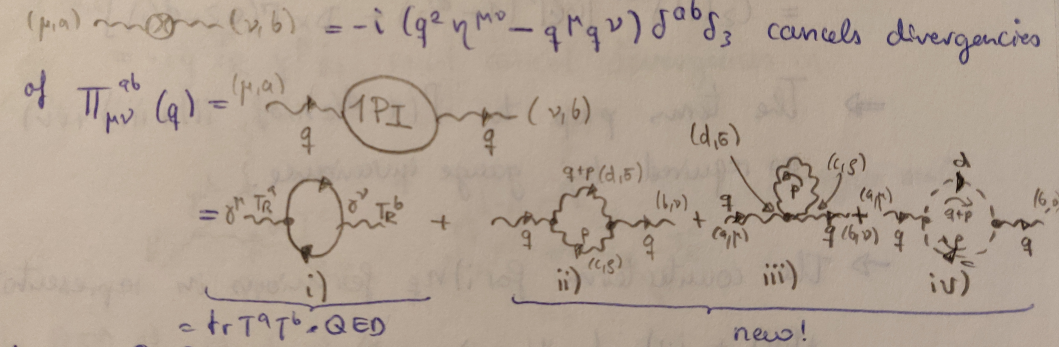
\includegraphics[width=0.5\linewidth]{gfx/YMpictures/YMselfenergy}
	\caption{YM self-energy renormalization}
	\label{fig:ymselfenergy}
\end{figure}
As in QED, \begin{equation}
q^\mu \Pi\munu(q)=0,
\end{equation}
which is a consequence of the Slavnov-Taylor identities. So we have
\begin{equation*}
	\Pi\munu(q)=i (q^2 \eta^{\mu \nu} - q^\mu q^\nu) \Pi(q^2).
\end{equation*}
Thus, compute the four diagrams $i)-iv)$ to find $\delta_3$:
\begin{enumerate}
	\item[i)] Choosing $\Delta:= -x(1-x)q^2$ with renormalization scale $\mu$, we find
	\begin{equation}
	\delta_3 |_{i)} = -\frac{g^2}{(4 \pi)^2} \frac{4}{3} C(R) \frac{\Gamma(2-\frac{\md}{2})}{(\mu^2)^{2-\frac{\md}{2}}}
	\end{equation}
	for a fermion in representation $R$.\\
	\\
	Note that the pure YM diagrams $ii)-iv)$ (pure in the sense that they do not appear in QED) are computed in Feynman gauge $\xi=1$.
	\item[ii)] Contains two types of divergences, via dimensional Regularization:
	\begin{enumerate}
		\item $\Gamma(2-\frac{\md}{2})\times \dots \leftrightarrow$ corresponds to logarithmic divergences in $\md=4$.
		\item $\Gamma(1-\frac{\md}{2})\times \dots \leftrightarrow$ corresponds to logarithmic divergence in $\md=2$, i.e. $\int \frac{\md^{\md} p}{(p^2)}$ and thus a quadratic divergence in $\md=4$.
	\end{enumerate}
	A quadratic divergence would indicate a renormalization of the gauge boson mass, which is forbidden by gauge invariance. This term must hence cancel against other contributions.
	\item[iii)]
	\begin{equation}
	iii)= \left[A \cdot \Gamma(1-\frac{\md}{2}) + B\cdot \Gamma(2-\frac{\md}{2}) \right] C_2(H) \delta^{ab} 
	\end{equation}
	\item[iv)]
	We get a $(-1)$ sign from Grassman fields in loop
	\begin{align}
		iv)&= (-1) \int \frac{\md^4p}{(2 \pi)^4} \frac{i}{p^2} \frac{i}{(p+q)^2} g^2 f^{dac} (p+q)^\mu f^{cbd} p^\nu \nonumber \\
		&= C_2(H) \delta^{ab} \left[C \cdot \Gamma(1-\frac{\md}{2}) + D\cdot \Gamma(2-\frac{\md}{2})\right].
	\end{align}
\end{enumerate}
The terms proportional to $\Gamma(1-\frac{\md}{2})$ of $ii)+iii)+iv)$ precisely cancel - as required by gauge invariance.
\\
Thus, the counterterm for $1)$ $n_f$ fermions in Representation $R_f+2)+3)+4)$ (with $\Delta= \mu^2$) is
\begin{equation}
\delta_3 = \frac{g^2}{(4 \pi)^2} \frac{\Gamma(2-\frac{\md}{2})}{(\mu^2)^{2-\frac{\md}{2}}} \left[\frac{5}{3} C_2(H) - \frac{4}{3} n_f C(R_f)\right].
\end{equation}



\subsubsection{Computation of $\delta_2$}

\begin{figure}[h!]
	\centering
	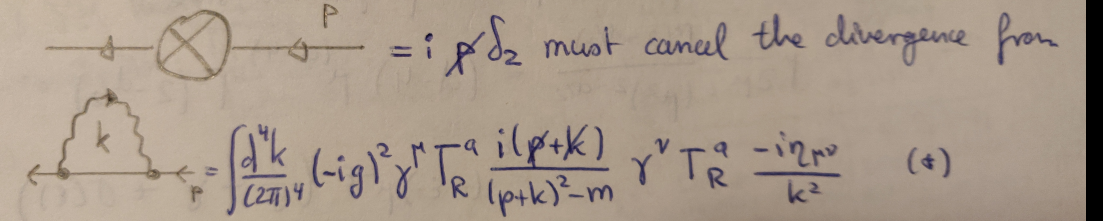
\includegraphics[width=0.7\linewidth]{gfx/YMpictures/YMoneLoopDelta2}
	\caption{}
	\label{fig:ymoneloopdelta2}
\end{figure}
Since we only need the UV divergences, we set again $m=0$.
\\The group theory factor is $T^a_R T^a_R = C_2(R) \cdot \mI$, thus
\begin{align}
	\ref{fig:ymoneloopdelta2} &= C_2(R)\mI  \times \left(\feynmandiagram[horizontal=a to b]{a--c--d--b, c--[boson, half left]d};\right)|_{QED} \\
	&= C_2(R) \frac{i g^2}{(4 \pi)^{\frac{\md}{2}} } \slashed{p} \int_0^1 \md x (1-x)(\md -2 ) \frac{\Gamma(2-\frac{\md}{2})}{\Delta^{2-\frac{\md}{2}}}
\end{align}
with $\Delta=-x(1-x)p^2$.\\ 
Identifying $\Delta=\mu^2$ yields
\begin{equation}
\delta_2 = - \frac{g^2}{(4 \pi)^2} \frac{\Gamma(2-\frac{\md}{2})}{(\mu^2)^{2-\frac{\md}{2}} } C_2(R).
\end{equation}


\subsubsection{Computation of $\delta_1$}
\begin{figure}[h!]
	\centering
	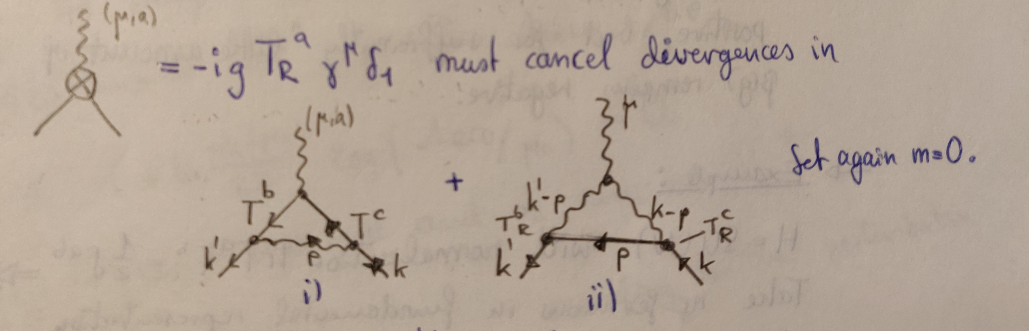
\includegraphics[width=0.7\linewidth]{gfx/YMpictures/YMoneLoopDeltaOne}
	\caption{}
	\label{fig:ymoneloopdeltaone}
\end{figure}
Consider the two separate diagrams individually
\begin{enumerate}
	\item[i)] In QED the Ward identities imply $\delta_1 |_{QED} = \delta_2|_{QED}$. We can factorize the diagram into contributions from YM and QED similar interactions like the following with this identity
	\begin{equation}
	\delta_1 |_{i)} = \underbrace{- \frac{g^2}{(4 \pi)^2} \frac{\Gamma(2-\frac{\md}{2})}{(\mu^2)^{2-\frac{\md}{2}} }}_{= T^a_R \cdot ({i)}_{QED})} \left(C_2(R)-\half C_2(H)\right),
	\end{equation}
	where we used the results from our QED calculations and just included the group theory factor..
	\item[ii)] Applying the same logic here, we find
	\begin{equation}
	\delta_1 |_{ii)} = -\frac{g^2}{(4 \pi)^2} \frac{\Gamma(2-\frac{\md}{2})}{(\mu^2)^{2-\frac{\md}{2}} } \frac{3}{2} C_2(H).
	\end{equation}
\end{enumerate}
Altogether
\begin{equation}
\delta_1 = - \frac{g^2}{(4 \pi)^2} \frac{\Gamma(2-\frac{\md}{2})}{(\mu^2)^{2-\frac{\md}{2}}} \left[C_2(R)+C_2(H)\right].
\end{equation}

\subsubsection{YM  $\beta$-function at $1$-loop in $g$}
The final result is found by noting that the divergencies vanish for the computation of the $\beta$-function since
\begin{align*}
	\mu \frac{\partial}{\partial \mu} \frac{\Gamma(2 -\frac{\md}{2})}{(\mu^2)^{2-\frac{\md}{2}} } &= (\md -4) \mu^{(\md-4)} \Gamma(2-\frac{\md}{2}) \\
	&\stackrel{\md=4-\epsilon}{=} (-\epsilon) \mu^{-\epsilon} \left(\frac{2}{\epsilon} -\gamma + \mO(\epsilon)\right) \\
	&\stackrel{\epsilon\rightarrow 0}{=} -2.
\end{align*}
\begin{mybox}{YM $\beta$ function to leading order in $\md=4$}
	\begin{equation}
	\label{eq:betafunctionYangMills}
	\beta^{(1)}_{YM}(g) = - \frac{g^3}{(4 \pi)^2} \left[\frac{11}{3} C_2(H) - \frac{4}{3} n_f C(R_f)\right].
	\end{equation}
\end{mybox}



\subsection{Fourth example for On-shell renormalization -- QCD renormalized}
\label{subsec:renormalizationqcd}
\subsubsection{Superficially divergent vertex functions in QCD}
Again, the logic is to renormalize divergent $1PI$ graphs. To find these we employ again power-counting via SDOD \ref{eq:renormalizationSdodQCD} and will look at the explicit symmetries of the theory to nail down the graphs which are actually divergent.
\begin{enumerate}
\item \feynmandiagram[horizontal=a to b]{a--[gluon] v1 --[gluon] v2 [particle=$(1PI)$] --[gluon] v3 --[gluon] b }; \quad D=2.
\item \feynmandiagram[horizontal=a to b]{a--[fermion] v1 --[fermion] v2 [particle=$(1PI)$] --[fermion] v3 --[fermion] b }; \quad D=1.
\item \feynmandiagram[horizontal=a to b]{a--[scalar] v1 --[scalar] v2 [particle=$(1PI)$] --[scalar] v3 --[scalar] b }; \quad D=2.
\item \feynmandiagram[horizontal=a to b]{a--[fermion] v1 --[fermion] v2 [particle=$(1PI)$] --[gluon] v3 --[gluon] b, c --[fermion] v2 }; \quad D=0.
\item \feynmandiagram[horizontal=a to b]{a--[gluon] v1 --[gluon] v2 [particle=$(1PI)$] --[gluon] v3 --[gluon] b, c --[gluon] v2 }; \quad D=1.
\item \feynmandiagram[horizontal=a to b]{a--[scalar] v1 --[scalar] v2 [particle=$(1PI)$] --[gluon] v3 --[gluon] b, v2 --[scalar] c }; \quad D=1.
\item \feynmandiagram[horizontal=a to b]{a--[gluon] v1 --[gluon] v2 [particle=$(1PI)$] --[gluon] v3 --[gluon] b, c --[gluon] v2, v3--[gluon] d }; \quad D=0.
\item \feynmandiagram[horizontal=a to b]{a--[gluon] v1 --[gluon] v2 [particle=$(1PI)$] --[gluon] v3 --[gluon] b, v2 --[scalar] c, d --[scalar] v3 }; \quad D=0, this one is not actually divergent..
\end{enumerate}
Note that we have more divergent amplitudes than free parameters in the theory. QCD is however renormalizable as the beta-function is non-negative. Therefore, some of these divergent graphs are actually finite by virtue of some symmetry of QCD. For example, the Slavnov-Taylor identities of QCD \todo{reference slavnov taylor} ensure that $g_s$ is \emph{universal}.\\
We can therefore pick any of the vertices to renormalize $g_s$. In literature, people normally pick diagram $6)$ is it is easier to work with scalar Grassmann-valued ghosts than with the Dirac algebra of the fermions. \\
Note that the vertices are the real problem, which tells us that we have a parameter free theory.
\subsubsection{Isolate divergences of all the self-energies at one loop}
We will express everything in terms of the bubble graph $B_0$ which in the UV is basically $B_0 |_{UV} = \frac{1}{\epsilon}$ in the limit of vanishing masses. This is therefore more a discussion of divergence behaviour in the UV and we will only give crude details to calculations. Let us start with regularizing the divergent graphs via dimensional regularization.
\begin{enumerate}
	\item Consider the quark self-energy at one loop. 
	\begin{align*} 
	&\hspace{-2.4cm}\feynmandiagram[horizontal=a to b]{a [particle=$i$] -- [fermion,momentum=\(k\)] v1 --[fermion] v2 -- v3 -- [fermion] b [particle=$j$], v1 --[gluon, half left, momentum=\(q-k\)] v2  }; = i \Sigma^{q \bar{q}} (k) =i \slashed{k} \Sigma^{q \bar{ q}} (k^2) + i \underbrace{m_q}_{=0} \Sigma^{q \bar{q}}_s (k^2)\\
	&\stackrel{\xi=1}{=} C_F \frac{i}{(4 \pi)^2} \frac{(2 \pi \mu)^{4-\md}}{ i \pi^2} \int \md^d q (-ig_s \gamma_\mu)  \\
	&\frac{i \slashed{q}}{q^2+i\epsilon} (-i g_s \gamma_\nu) \frac{-i g^{\mu \nu}}{(q-k)^2+i \epsilon} \delta^{ij}\\
	&=\left[\feynmandiagram[horizontal=a to b]{a -- [fermion] v1 --[fermion] v2 -- v3 -- [fermion] b [particle=$QED$], v1 --[boson, half left] v2 };\right]_{e^2 Q^2 \rightarrow g^2_s C_F} 
	\end{align*} 
Such that the quark self-energy at one-loop is
\begin{align}
	\label{eq:renormalizationQCDquarkselfenergy}
	 \Sigma^{q \bar{ q}}_V(k^2) &= \frac{\alpha_s}{4 \pi} C_F [B_0(k^2,0,0) -1] \delta^{ij} \\
	\Sigma^{q \bar{ q}}_V(k^2) |_{UV} &= \frac{\alpha_S}{4 \pi} C_F \frac{1}{\epsilon} \delta^{ij}\nonumber.
	\end{align}
where $V$ indicates the vector (ito indices) part and $S$ indicates the scalar component, this decomposition is in general possible.\\
As before, we use Dyson resummation to find the full propagator including all correction i.e. the \emph{dressed propagator}.
\begin{align*}
	\feynmandiagram[horizontal=a to b]{a --[fermion] v[particle=$(1PI)$]--[fermion]b }; &= 	\feynmandiagram[horizontal=a to b]{a --[fermion] b };+\feynmandiagram[horizontal=a to b]{a  --[fermion] v[particle=$\Sigma$]--[fermion]b }; + \dots \\
	&= \frac{1}{i (\slashed{p}-m)} \sum_{n=0}^{\infty} \left[i \Sigma^{q \bar{q}} \frac{1}{i (\slashed{p}-m)}\right]^n = \frac{i}{\slashed{p}-m+\Sigma^{q\bar{q}}(k)} \\
	&= i \frac{\slashed{p}[1+\Sigma^{q\bar{q}}_V] + m [1-\Sigma^{q\bar{q}}_s]}{p^2 -m^2 \left[\frac{1-\Sigma^{q \bar{q}}_s}{1+\Sigma^{q \bar{q}}_V}\right]} [1 + \Sigma^{q \bar{q}}_V]^2
\end{align*}
Note that the radiative corrections introduce a shift in the mass. This is still the non-renormalized dressed propagator, the shift in mass is infinite. 
\item Consider the gluon self-energy at one loop. We have
\begin{align*}
\Sigma^{A^a_\mu A^b_\nu} (k^2) &= \feynmandiagram[horizontal=a to b]{a --[gluon] v1--[half left] v2 -- [gluon] b, v2--[half left] v1};+  \feynmandiagram[horizontal=a to b]{a --[gluon] v1--[gluon,half left] v2 -- [gluon] b, v2--[gluon, half left] v1}; \\
&+ \feynmandiagram[horizontal=a to b]{a --[gluon] v1--[scalar, half left] v2 -- [gluon] b, v2--[scalar, half left] v1}; + \feynmandiagram[horizontal=a to b]{a --[gluon] v1-- [gluon] b, v1--[loop,gluon] v1};
\end{align*}
where we will look at the different contributions separately.
We have
\bse 
 \feynmandiagram[horizontal=a to b]{a --[gluon] v1--[half left] v2 -- [gluon] b, v2--[half left] v1}; = \left[ \feynmandiagram[horizontal=a to b]{a --[boson] v1--[half left] v2 -- [boson] b[particle=$QED$], v2--[half left] v1};\right]_{e^2 Q^2 \rightarrow q^2_s T_F} 
\ese 
which is automatically transverse\footnote{This is something we have to check in QCD by BRST symmetry, as radiative corrections should never generate a longitudinal mode.}.
\bse 
\feynmandiagram[horizontal=a to b]{a --[gluon] v1-- [gluon] b, v1--[loop,gluon] v1}; \propto \int \md^d a \frac{1}{q^2} = 0 
\ese 
which vanishes as this integral is scale-less\footnote{in dim. Reg., scale-less integrals vanish.}. The gluon bubble has 
\bse 
 \feynmandiagram[horizontal=a to b]{a --[gluon] v1--[gluon,half left] v2 -- [gluon] b, v2--[gluon, half left] v1}; =  i C_A \delta^{ab} \frac{\alpha_s}{8 \pi} k^2 \left\{ g\munu\left[\frac{19}{6} B_0 + \frac{1}{9}\right] - \frac{k_\mu k_\nu}{k^2} \left[\frac{11}{3} B_0 + \frac{1}{9}\right]    \right\}
\ese 
which is not transverse as the prefactors of the generally possible decomposition
\bse 
X\munu = A g\munu + B\frac{k_\mu k_\nu}{k^2}
\ese 
do not agree, i.e. transverse if $\abs{A}=\abs{B}$. This becomes transverse when we add the ghost loop, which is
\bse 
 \feynmandiagram[horizontal=a to b]{a --[gluon] v1--[scalar, half left] v2 -- [gluon] b, v2--[scalar, half left] v1}; = i C_A \delta^{ab} \frac{\alpha_s}{8 \pi} k^2 \left\{g\munu \left[\frac{1}{6} B_0 + \frac{1}{9}\right] - \frac{k_\mu k_\nu}{k^2} \left[-\frac{1}{3} B_0 + \frac{1}{9}\right] \right\}.
\ese 
This is as well not transverse, but adding the contributions up yields a transverse self-energy
\begin{align*}
	\Sigma^{A^a_\mu A^b_\nu }(k) &= N_f T_f \delta^{ab} \frac{\alpha_s}{3 \pi} k^2 (g\munu - \frac{k_\mu k_\nu}{k^2}) (B_0 - \frac{1}{3}) \\
	& -C_A \delta^{ab} \frac{\alpha_S}{4 \pi} k^2 (g\munu - \frac{k_\mu k_\nu}{k^2}) (\frac{10}{3} B_0 + \frac{2}{9})
\end{align*}
which is transverse.
Decomposing this again into transverse and longitudinal direction, we find that the longitudinal direction vanishes and that the resulting transverse singularity in the UV looks like
\be 
	\label{eq:renormalizationQCDGluonselfEnergy}
\Sigma^{AA}_T |_{UV} =\left[ \frac{\alpha_S}{3 \pi } T_f N_f k^2 - \frac{5 \alpha_s}{12 \pi} C_A k^2 \right]\frac{1}{\epsilon}.
\ee 
Introduce the \emph{vacuum polarization}
\bse 
\Pi^{AA}(k^2) = \frac{\Sigma^{AA}_T(k^2)}{k^2}.
\ese 
The dressed gluon propagator therefore is given by
\be 
\feynmandiagram[horizontal=a to b]{a--[gluon] v [blob] -- [gluon] b}; = \frac{-i}{k^2 \left[1 + \Pi^{AA}(k^2)\right]} \left(g\munu -\frac{k_\mu k_\nu}{k^2}\right) - \xi \frac{i}{k^2} \frac{k_\mu k_\nu}{k^2}
\ee 
where there is no shift in the pole, i.e. the gluon does not have a mass as dictated by gauge invariance.
\item Consider the quark-gluon vertex at one-loop
\bse 
-i g_s \Lambda^a_\mu (p,\bar{p})= \feynmandiagram [small, horizontal=a to p1] {
	a -- [gluon] t1 -- t2 --[gluon] t3 -- t1,
	t2 --  p1 [particle=\(p\)],
	t3 -- p2 [particle=\(\bar{p}\)],
	p1 -- [opacity=0.2] p2,
};
+
\feynmandiagram [small, horizontal=a to p1] {
	a -- [gluon] t1 -- [gluon]t2 -- t3 --[gluon] t1,
	t2 --  p1 [particle=\(p\)],
	t3 -- p2 [particle=\(\bar{p}\)],
	p1 -- [opacity=0.2] p2,
};
\ese\footnote{As long as this diagram is not fixed, note that this is basically the gluon-quark vertex where you get an internal interaction with either two fermions one gluon or two gluons and one fermion, where the later is not present in QED.}
where the latter diagram is not present in QED. These diagrams are difficult to solve. We go into the high energy limit $q^2 \rightarrow \infty$ to approximate solutions and simplify our life as we are only interested in the UV behaviour. One finds
\be 
\label{eq:renormalizationQCDVertex}
\Lambda^a_\mu (p,\bar{p}) |_{UV} = t^a \gamma_\mu \frac{\alpha_s}{4 \pi} \frac{1}{\epsilon} \left[- \frac{T_f}{N_c} + 3 T_f N_c\right].
\ee 
\end{enumerate}
Now we have the divergent behaviour of all self-energies and of the vertex. We are therefore done with regularizing the theory. Now we renormalize. We choose the $\bar{MS}$ scheme for this and will find the renormalized strong coupling in the end.
\subsubsection{Renormalization of QCD divergent graphs}
As described above, we now do the following decomposition
\begin{align*}
	\text{(divergent) bare quantities} =& \text{(finite) renormalized quantity} \\
	&\times \text{(divergent) renormalization constant},
\end{align*}
where the renormalization constants \ref{eq:wavefunctionrenormalization} $Z_x$ are dimension-less\footnote{This is a convenient redefinition to cancel factors in LSZ}. We have
\begin{align*}
	A^a_{\mu,0} &= \sqrt{Z_A} A^a_\mu, \quad \psi_{q,0} = \sqrt{Z_q} \psi_q, \quad g_{s,0} = \mu^\epsilon Z_{g_s} g_s \\
	m_{q,0} &= Z_{m_q} m_q, \quad \xi_0 = Z_\xi \xi.
\end{align*}
We can now do the perturbative expansion in the wavefunction renormalization in terms of $Z_x = 1 +\delta Z_x$, compare \ref{eq:wavefunctionrenormalization} for scalar theory, i.e.
\bse 
\phi_0 = \sqrt{Z_\phi} \phi = (1 + \half \delta Z_\phi) \phi, \; \lambda_0 = Z_\lambda \lambda = (1+\delta Z_\lambda) \lambda,\quad \lambda=\xi,g_s,\dots; \phi=A_\mu,\psi,\dots 
\ese
to first order, which is the only one we need as we only computed the divergent graphs to first order.\\
Now we introduce renormalized quantities and counterterms, where the latter contain $\delta Z_x$
\bse 
\mL(\phi_0,\lambda_0) = \mL_r (\phi,\lambda) + \mL_{ct} 
\ese 
such that we do not \emph{add} counterterms, we just reparametrize the Lagrangian.\\
From this one finds Feynman rules for the counterterms
\begin{align*}
	\feynmandiagram[horizontal=a to b]{a --[gluon] v[crossed dot] --[gluon] b}; &= i \delta^{ab} \delta Z_A k^2 (g\munu -\frac{k_\mu k_\nu}{k^2} ) + i \delta^{ab} \frac{1}{\xi} k_\mu k_\nu (\delta Z_\xi - \delta Z_A) \\
	\feynmandiagram[horizontal=a to b]{a--[fermion] v [crossed dot] --[fermion] b }; &= i \delta_Z (\slashed{p}-m_q) - i \delta m_q, \quad \delta m_q := \delta Z_{m_q} m_q \\
	\feynmandiagram[horizontal=a to b]{a --[gluon] v [crossed dot]--[fermion] b, c--[fermion] v}; &=	\feynmandiagram[horizontal=a to b]{a --[boson] v [crossed dot]--[fermion] b, c--[fermion] v}; \left[\delta Z_{g_s} + \delta Z_q + \half \delta Z_A\right].
\end{align*}
Now we do perturbation theory around renormalized quantities to find the renormalized vertex functions.\\
Let $\hat{A}$ denote a renormalized quantity, then we find the following renormalized $1PI$ graphs and counterterms.
For this we need that the dressed propagator now has the form 
\bse 
\feynmandiagram[horizontal=a to b]{a -- v[blob] -- b}; = \feynmandiagram{a--b}; + \feynmandiagram{a -- v [particle=$1PI$]--b }; + \feynmandiagram{a--v [crossed dot] --b}; + \dots 
\ese 
such that we rewrite the self-energies and vertex we find above with the counterterms introduced to deduce the renormalized self-energies and vertex.
\begin{enumerate}
	\item 
	\begin{align*}
		\feynmandiagram[horizontal=a to b]{a --[gluon] v [particle=$1PI$] -- [gluon] b}; &=-i \delta^{ab} \left(g\munu - \frac{k_\mu k_\nu}{k^2}\right) \left[k^2 + \underbrace{\Sigma^{AA}_T(k^2)+k^2 \delta Z_A}_{=: \hat{\Sigma}^{AA}_T(k^2) \text{ (II)} }\right] \\
		&_ i \delta^{ab} \frac{k_\mu k_\nu}{k^2} \frac{1}{\xi} \left[k^2 + \underbrace{\xi \overbrace{\Sigma^{AA}_L(k^2)}^{=0 \text{ long. decouples}}+ k^2 (\delta Z_A-\delta Z_\xi)}_{=: \xi \hat{\Sigma}^{AA}_L(k^2) \text{ (1)} }\right]\\
		(I)\Rightarrow \quad \delta Z_\xi &=  \delta Z_A \quad \Rightarrow \hat{\Sigma}^{AA}_L(k^2) \stackrel{!}{=0} \\
		(2)\Rightarrow \quad \delta Z_A &= - \frac{\Sigma^{AA}_T}{k^2} |_{\bar{UV}} = - \Pi^{AA}_P |_{\bar{UV}} = - \frac{\alpha_s}{4 \pi} \frac{1}{\bar{ \epsilon}} \left[ \frac{4}{3} T_f N_f - \frac{5}{3} C_A\right] \\
		\bar{\epsilon} &:= \frac{1}{\epsilon} - \gamma_E + \ln(4\pi).
	\end{align*}
\item 
\begin{align*}
	\feynmandiagram[horizontal=a  to b]{a --v [particle=$1PI$] -- b}; &= i \slashed{p} \left[1 + \underbrace{\Sigma^{q \bar{q}}_V (k^2) +\delta Z_q}_{=:\hat{\Sigma}^{q \bar{q}}_V(k^2) \text{ (3)}} \right]\\
	(3)\Rightarrow \quad \delta Z_q &= - \Sigma^{q\bar{ q}}_V (k^2) |_{\bar{UV}} = - \frac{\alpha_s}{4 \pi} C_F \frac{1}{\bar{\epsilon}}.
\end{align*}
\item 
\begin{align*}
	\feynmandiagram[horizontal=a to b]{a --[gluon] v [particle=$1PI$] -- b, v--c}; &= -i g_s t^a \gamma_\mu - ig_s \underbrace{\left[\Lambda^a_\mu (p,\bar{p}) + t^a \gamma_\mu (\delta Z_{g_s} + \delta Z_q + \half \delta Z_A) \right]}_{=: \hat{\Lambda}^a_\mu(p,\bar{p}) \text{ (4)} }\\
		(4) \Rightarrow \quad \delta Z_{g_s} &= \frac{\alpha_s}{4\pi} \frac{1}{\bar{\epsilon}} \left[ \frac{N_f}{3} - \frac{11}{6} C_A\right].
\end{align*}
\end{enumerate}
\subsubsection{Running coupling and beta-function}
First and foremost a warning, the concept of running coupling, renormalization scale and $\beta$-function has already been discussed in \ref{subsec:renormalizationqed}, but has not been generally defined. All of this comes after this section when we talk about renormalization flow in detail.\\
With the counterterms known, we can now infer the $\beta$-function of QCD at one-loop. Note that the $\mu$-dependence introduced before is completely arbitrary. $\mu$ is normally called \emph{renormalization scale} and is discussed in more detail in the following \ref{eq:callansymanzik}. The arbitrariness of $\mu$ implies that explicit and implicit $\mu$-dependencies have to cancel.
One can do an expansion of the $\beta$-function to all orders in perturbation theory
      \be 
      \beta(\alpha_s) := \frac{\md \ln \alpha_s}{\md \ln \mu^2} = - \sum_{n=1}^{\infty} \beta_{n-1} \left(\frac{\alpha_s}{2 \pi}\right)^n= - \beta_0 \frac{\alpha_s}{2\pi}- \dots
      \ee 
      where we find the first order result via
      \bse 
      \beta_0 = g_s \frac{\md Z^{(1)}_{g_s}}{\md g_s} = 2 \frac{g^2_s}{(4 \pi)^2},\quad Z_{gs} = \sum_{n=1}^{\infty} \frac{1}{\epsilon^n} Z^{(1)}_{g_s}
      \ese  
      to be 
      \be 
      \beta_0 = \frac{11}{6} C_A  - \frac{N_f}{3}.
      \ee 
      Note that $\beta_0 >0$ for $N_f \geq 16$, which is experimentally known. Therefore, $\alpha_s=\frac{g^2_s}{4 \pi}$ decreases for higher scales, this phenomenon is known as \emph{asymptotic freedom}.
      This result is also derived in \ref{eq:betafunctionYangMills} and discussed in more detail in \ref{subsec:qcdrunningcoupling}.
      








\subsection{Renormalization flow (Callan-Symanzik flow)}
\subsubsection{The renormalization scale}
\begin{mybox}{The renormalization scale}
	
	Renormalization automatically introduces a mass scale $\mu$ - \emph{the renormalization scale} - into the quantum theory via the renormalization conditions (even when the classical theory was scale-free).\\
	The renormalization scale can be an independent scale since the renormalization conditions are arbitrary.
\end{mybox}
\subsubsection{The renormalization conditions stated}
\begin{mybox}{Renormalization conditions}
Renormalization forces the introduction of a scale at which the renormalization conditions are imposed, e.g. for $\phi^4$ we could generally impose
\begin{align}
	M^2(p^2)|_{p^2=-\mu^2} &\stackrel{!}{=} 0 \\
	-i \mM(p_1,\dots,p_4) |_{s,t,u=-\mu^2} &\stackrel{!}{=} -i \lambda 
\end{align}
such that or with ??
\begin{equation}
	M^2(p^2) = \frac{\lambda^2}{\Lambda^2} \frac{p^2}{(4\pi)^4} \left[\ln \frac{p^2}{-\mu^2} -1\right] - \frac{\mu^2 \lambda^2}{12 (4\pi)^4}.
\end{equation}
Renormalization conditions away from $p^2=m^2$ become necessary in massless theories where the measurement that determines the renormalization scale can not be done at $p^2=0$.
\end{mybox}
\begin{mybox}{Renormalization conditions}
	We have as many renormalization conditions as we find superficial amplitudes. However, $\feynmandiagram{b [blob]};$ is absorbed in $V_0$ ground state energy such that it doesn't have a renormalization condition.\\We have
	\begin{align}
		\feynmandiagram[horizontal=a to b]{a--c [particle=$1PI$]--b};|_{p^2=m^2} &\stackrel{!}{=} \frac{i}{p^2-m^2}
	\end{align}
	which implies three renormalization conditions
	\begin{enumerate}
		\item Pole position should be the physical mass.
		\item The residue of pole $=1$.
		\item $\lambda$ is coupling at same scale: $s=4m^2, u=t=0.$ I.e. fix your mass scale.
	\end{enumerate}
	These translate to the three equivalent conditions
	\begin{align}
		1) \quad M^2 (p^2) |_{p^2=m^2} \stackrel{!}{=}& 0\\
		2) \quad \frac{\md}{\md p^2} M^2(p^2) \stackrel{!}{=}&0 \\
		3) \quad i M(p_1 p_2 \rightarrow p_3 p_4) |_{p^2=0} \stackrel{!}{=}&-i \lambda,\\
		\text{where} \; p^2=0 \Leftrightarrow 4m^2&=s \text{ and } t=u=0.\nonumber
	\end{align}
	These conditions are deduced from the fully resummed propagator
	\begin{align*}
		\feynmandiagram[horizontal=a to b]{a--c[blob]--b}; &= \underbrace{\frac{i}{p^2-m^2-M^2(p^2)}}_{-iM^2(p^2) \text{ is amplitude of all 1PI amputated diagrams}} \\
		&= \feynmandiagram{a --b}; + \feynmandiagram[horizontal=a to b]{a--c--b, c -- [half left] c}; \\
		&+ \feynmandiagram[horizontal=a to b]{a --c[crossed dot] --b}; + \mO(\lambda^2),\\
		\Rightarrow \quad -iM^2(p^2)|_{\mO(\lambda)} &= \feynmandiagram[horizontal=a to b]{a--c--b, c -- [half left] c}; + \feynmandiagram[horizontal=a to b]{a --c[crossed dot] --b}; \\
		&=-\frac{i\lambda}{2}\int \frac{\md^4k}{(2 \pi)^4} \frac{i}{k^2-m^2+i\epsilon}+i (p^2 \delta_Z-\delta_m) \\
		&= \feynmandiagram[horizontal=a to b]{a--c[particle=$1PI$]--b};.
	\end{align*}
\end{mybox}
Most often we renormalize $\phi_r=Z^{-\half} \phi_0$ with the wavefunction renormalization factor $Z$ as the residue of the propagator at the physical mass $p^2=m^2$. We impose in this context the renormalization condition
\begin{equation}
	M^2(p^2) |_{p^2=m^2} = 0 = \frac{\md}{\md p^2} M^2(p^2) |_{p^2=m^2}
\end{equation}
and
\begin{equation}
	\feynmandiagram[vertical=a to b]{a--c[blob]--d, b--c--e}; = -i \lambda 
\end{equation}
at scale $s=4m^2, t=u=0$, which implies $\mu=m$, in order to specify the counterterms $\delta_Z,\delta_m,\delta_{\lambda}$ appearing due to the renormalization. These will then cancel the divergences of higher order diagrams (BPHZ).
\subsubsection{Derivation of renormalization conditions}
How to find the renormalization conditions, consider the self-energy
\begin{equation*}
	\feynmandiagram{a--v[blob] --b};= \frac{i}{p^2-m^2_{\phi}} +\text{ regular at }p^2=m^2\left\{  \begin{array}{ll}
		1)\;p^2=m^2_{\phi} & \text{ pole}\\
		2)\;\text{residue at } &p^2=m^2 \text{ is }1\\
	\end{array}  \right\}
\end{equation*}
these renormalization conditions fix the mass of the particle, thus the mass scale.\\
Now we Taylor expand this self-energy
\begin{align*}
	&= \frac{i}{p^2-m^2_{\phi}-\Sigma_\phi(m^2) -(p^2-m^2_\phi) \frac{\md \Sigma_\phi}{\md p^2} -(p^2-m^2_\phi)^2 \frac{\md^2 \Sigma_\phi}{\md (p^2)^2} +\dots}\\
	&1) \Rightarrow\; \feynmandiagram{a--v[blob] --b};|_{p^2=m^2} \stackrel{!}{=} \infty \;\Rightarrow \; \Sigma_\phi(m^2)\stackrel{!}{=} 0\\
	&\text{which gives}  \text{ us the first renormalization condition. Further looking at }\\
	&2) \Rightarrow \;\feynmandiagram{a--v[blob] --b}; = \frac{i}{(p^2-m^2_\phi) \left[1-\underbrace{\frac{\md \Sigma}{\md p^2}(m^2_\phi)}_{\stackrel{!}{=}0} - \underbrace{(p^2-m^2\phi) \frac{\md^2 \Sigma}{\md(p^2)^2} (m^2_\phi)}_{|_{p^2=m^2} \stackrel{!}{=}0}+\dots \right]}\\
	&\text{give us }\text{ the second and third renormalization condition.}
\end{align*}










\subsubsection{The Callan-Symanzyk (CS) equation (renormalization flow equation)}
\marginpar{$G_n(x_1,\dots,x_n)=G_n(x,\lambda,m,\mu)$}
\begin{mybox}{The Callan-Symanzyk equation}
	To quantify the dependence of coupling constants on the renormalization scale $\mu$, we can study the Callan-Symanzik (or renormalization group) equation. The $\mu$ independence of $n$-point correlation function computed in bare perturbation theory reads 
	\begin{equation}
		\frac{\md}{\md \mu} G_{n,0} (p;\lambda,m\mu) = 0,
	\end{equation}
	whereas the $\mu$ independence of $n$-point correlation function computed in renormalized perturbation theory reads
	\begin{equation}
		\frac{\md }{\md \mu} \left[Z^{\frac{n}{2}} G_n(p;\lambda,m,\mu)\right] =0.
	\end{equation}
	The Callan-Symanzik equation reads
	\begin{equation}
		\label{eq:callansymanzik}
		\left(\mu \frac{\partial}{\partial \mu} + \beta(\lambda) \frac{\partial}{\partial \lambda} + n \gamma_{\phi}(\lambda) + \beta(m) \frac{\partial}{\partial m^2}\right) G_n(p;\lambda,m,\mu) =0
	\end{equation}
	with 
	\begin{align}
		\beta(\lambda) &:= \mu \frac{\md \lambda}{\md \mu} |_{\lambda_0,m_0}, \quad \beta(m) := \mu \frac{\md m^2}{\md \mu} |_{\lambda_0,m_0}\\
		\gamma_{\phi}(\lambda)&:= \half \frac{\md}{\md \mu} \ln Z |_{\lambda_0,m_0}.
	\end{align}
To obtain the functions $\beta(\lambda),\gamma_{\phi}(\lambda)$ and $\beta(m)$ we compute $n$-point correlation functions up to a given order and find a convenient set of correlation functions we can extract sufficiently much information from.
\end{mybox}
\begin{mybox}{The $\beta$ function}
	$\beta_{\lambda}$ for example describes how the physical coupling $\lambda$ changes as we change the energy scale $\mu$ at which we can perform an experiment.\\
	The CS equation allows us to (perturbatively) compute $\beta_{\lambda},\beta_{m^2},\gamma_{\phi}$ explicitly by first computing$G_n(x_1,\dots,x_n)$ and then plugging it into the CS equation:\\
	E.g. \begin{equation}
		\beta_{\lambda} = \frac{3\lambda^2}{16 \pi^2} + \mathcal{O}(\lambda^3)<s
	\end{equation}
	for massless $\phi^4$ theory.
\end{mybox}
E.g. for massless $\phi^4$-theory at $1$-loop level, we find
\begin{equation}
	\gamma_{\phi}(\lambda) = \half \mu \frac{\partial}{\partial \nu} \delta_\phi 
\end{equation}
and because the $1$-loop contribution to $\delta_Z$ is the momentum-independent tadpole
\begin{equation}
(-i \lambda) \half \int_p \frac{i}{p^2-m^2}
\end{equation}
we only need $\delta_m$ in the counter diagram $i(p^2\delta \phi-\delta_m)$ to absorb the divergence, such that $\delta_\phi=Z-1=\mO(\lambda^2)$ and
\begin{equation}
	\gamma_\phi(\lambda) = \mO(\lambda^2)
\end{equation}
so we can neglect it to calculate the one-loop beta function (and vice versa) and the $4$-point function is completely sufficient to obtain
\begin{equation}
	\beta^{(1)}(\lambda) = \frac{-\mu \frac{\partial}{\partial \mu} G^{(1)}_4(p;\lambda,\mu)}{\frac{\partial}{\partial \lambda} G^{(1)}_4(p;\lambda,\mu)} = \mu \frac{\partial \lambda}{\partial \mu}
\end{equation}
which is a differential equation for $\lambda(\mu)$ which we can solve by simple integration as described in the following \ref{subsubsec:betafunc}
\subsubsection{$\beta$-function and running of dimensionless (renormalizable) couplings}
\label{subsubsec:betafunc}
\begin{mybox}{}
	$\beta$-function as derived (perturbatively) from the CS equation
	\begin{equation}
	\label{eq:betafunction}
		\beta(\lambda) = \mu \frac{\md}{\md \mu} \lambda(\mu)
	\end{equation}
	implicitly gives the complete scaling behaviour $\lambda(\mu)$ by integration of \ref{eq:betafunction}
	\begin{equation}
		\int_{\lambda^*}^{\lambda(\mu)} \frac{\md \lambda^\prime}{\beta(\lambda^\prime)} = \ln \frac{\mu}{\mu^*}.
	\end{equation}
\end{mybox}
Collecting results
\begin{enumerate}
	\item $\phi^4$ beta function
	\begin{equation}
		\beta^{(1)}(\lambda) = (d-4) \lambda + \frac{3 \lambda^2}{16 \pi^2} + \mO(\lambda^3),
	\end{equation}
	\item QED beta function
	\begin{equation}
		\beta^{(1)}(e) = \frac{e^3}{12 \pi^2} + \mO(e^4),
	\end{equation}
	\item QCD beta function
	\begin{equation}
		\beta^{(1)}(g) = -7 \frac{g^3}{16 \pi^2}+\mO(g^4),
	\end{equation}
	\item $SU(N)$ Yang-Mills beta function
	\begin{equation}
		\beta^{(1)}(g) = - (\frac{11}{3} N - \frac{2}{3} N_f) \frac{g^3}{16 \pi^2} + \mO(g^4),
	\end{equation}
	\item Lie group Yang-Mills beta function
	\begin{equation}
		\beta^{(1)}(g) = - (\frac{11}{3} C_2(Ad) - \frac{4}{3} N_f C(F)) \frac{g^3}{16 \pi^2} + \mO(g^4).
	\end{equation}
\end{enumerate}
\subsubsection{$\beta$-function of dimensionless (marginal) couplings from counterterms}
\begin{mybox}{}
	The generic form of connected $n$-point functions is
	\begin{equation}
	G_n = (\text{tree}) + (1\text{PI loop}) + (\text{vertex CT}) + ( \text{external propagators})
	\end{equation}
	or more concretely employing cut-off regularization $\Lambda$ for massless theory
	\begin{equation}
	G_n = \prod_i \frac{i}{p^2_i} \left[-i g - i B \ln \frac{\Lambda^2}{p^2} - ig \sum_j\left(A_j \ln \frac{\Lambda^2}{p^2_j} -\delta_{\phi_j}\right)\right]
	\end{equation}
	with some $\mu$ independent coefficients $A,B$, such that the Callan-Symanzik equation $\mu \frac{\md}{\md \mu}G_n=0$ implies with $\beta(g) \frac{\partial}{\partial}(\text{tree}) = \beta(g)$ at $1$-loop order
	\begin{equation}
		\beta(g) = \mu \frac{\partial}{\partial \mu} (-\delta_g + \half g \sum_j \delta_{\phi_j}).
	\end{equation}
	
\end{mybox}
For gauge theory and Yukawa theory (where $g$ is absorbed in $\delta_{\phi_j}$) the beta function of the fermion-fermion-boson coupling is simply
\begin{equation}
	\beta(g) = g \mu \frac{\partial}{\partial \mu} (-\delta_g+\delta_\psi + \half \delta_A).
\end{equation}


\subsubsection{Running of dimensionful (non/super-renormalizable couplings)}
\begin{mybox}{}
	Term with dimensionful coupling in the action
	\begin{equation}
		\int \md^d x C \mO(x) \subset S \text{ with } [C] = d- [\mO]
	\end{equation}
	e.g. $\mO(x) = \phi^6(x)$.
	\begin{equation}
		\left[\mu \frac{\partial}{\partial \mu} + \beta(\lambda) \frac{\partial}{\partial \lambda} + n \gamma_{\phi} + \beta_{\mO}(\lambda) \frac{\partial}{\partial g}\right]G_n(p;\lambda,C,\mu) =0
	\end{equation}
	with the general beta function for dimensionful coupling 
	\begin{equation}
		\beta_{\mO}(\lambda) := \mu \frac{\md g}{\md \mu} = (\gamma_{\mO}(\lambda) + [\mO] - d ) g(\mu) + (\text{diagrams}),
	\end{equation}
	where $g:=C\mu^{[\mO]-d}$, solution for $\gamma_{\mO}(\lambda)\rightarrow 0$ near the fixed point $\beta(\lambda^*)=0$,$\lambda^*=\lambda(\mu^*)$
	\begin{equation}
	\label{eq:asymptoticsolutionRunningdimensionfulcoupling}
		g(\mu) \propto g(\mu^*) \left(\frac{\mu}{\mu^*}\right)^{[\mO]-d}.
	\end{equation}
	We know
	\begin{align}
		&\mO \text{ is non-renormalizable } \Leftrightarrow [C]<0 \nonumber\\
		&\Leftrightarrow g^\prime(\mu) >0 \Leftrightarrow C \text{ is irrelevant in the IR}\\
		&\mO \text{ is super-renormalizable} \Leftrightarrow [C] >0 \nonumber \\
		&\Leftrightarrow g^\prime(\mu) <0 \Leftrightarrow C \text{ is relevant in the IR}.
	\end{align}
	
	
\end{mybox}
Note that for renormalizable couplings, i.e. $[C_i]=0$, the asymptotic solution \ref{eq:asymptoticsolutionRunningdimensionfulcoupling} does not give any scaling behaviour and is content free, $g(\mu) \propto g(\mu^*)$.

\subsection{The running coupling}
\subsubsection{Mathematically}
\begin{mybox}{}
	\begin{align}
		\beta(0) = 0 \text{ and } \beta(\lambda)>0 \; \forall \lambda& \quad \text{triviality}\\
		\beta(0)=0 \text{ and } \beta(\lambda)<0 \; \forall \lambda&\quad \text{ asymptotic freedom}\\
		\beta(\lambda)=0 \; \forall \lambda& \quad \text{ scale invariance }\\
		\exists \lambda^* \text{ st. } \beta(\lambda^*)=0 \text{ and } \beta^\prime(\lambda^*)<0& \; \text{asymptotic UV safety} \\
		\exists \lambda^* \text{ st. } \beta(\lambda^*)=0 \text{ and } \beta^\prime(\lambda^*) >0& \; \text{ asymptotic IR safety}.
	\end{align}
\end{mybox}
Note that
\begin{statements}
	Asymptotic freedom $\Rightarrow$ asymptotic UV safety.
\end{statements}
Consider some examples
\begin{enumerate}
	\item Triviality:\\
	$\phi^4$ and QED in $d=4$
	\item Asymptotic freedom:\\
	QCD in $d=4$ and $N_f<17$
	\item Scale invariance:\\
	conformal field theories and some SUSY theories
	\item Asymptotic UV safety:\\
	QCD in $d=4$ and $N_f <17$ and maybe quantum gravity
	\item Asymptotic IR safety:\\
	$\phi^4$ in $d<4$ and condensed matter theory
\end{enumerate}
\subsubsection{Conceptually}
\begin{mybox}{Renormalization group flow}
	The change in $\lambda(\mu)$ as we change $\mu$ is called \emph{renormalization group flow} or running coupling.\\
	$\lambda(\mu)$ gives the strength of the interaction at energy scale $\mu$.
\end{mybox}
The renormalization conditions define the meaning of the physical coupling $\lambda$ at the renormalization scale $\mu$.
\\
\\ E.g. in massless $\phi^4$-theory we defined the dimensionless coupling $\lambda$ by declaring that
\begin{equation}
	i M(p_1 p_2 \rightarrow p_3 p_4) = -i \lambda \quad at \quad s=t=u=-\mu^2.
\end{equation}
\begin{mybox}{Effective coupling}
	The so-defined coupling is therefore really a function of the renormalization scale $\mu, \lambda(\mu)$, and this $\lambda(\mu)$ is the \emph{effective coupling} relevant for processes with typical momenta of order $\mu$:
	\begin{statements}
		$\lambda(\mu)$ gives the strength of the interaction at energy scale $\mu$.
	\end{statements}
\end{mybox}
Depending on the sign of $\beta$ there are three qualitatively different renormalization group (RG) behaviours:
\begin{enumerate}
	\item If $\beta(\lambda) >0,  \lambda(\mu)$ increases as $\mu$ increases. If we start with a perturbative value $\lambda_0$ at $\mu_0$ and follow the RG flow for increasing $\mu$, then at some scale, $\lambda(\mu)$ ceases to be perturbative and perturbation theory is no more reliable. If by a non-perturbative analysis beyond that point one finds $\beta(\lambda) >0 \forall \lambda$, then $\lambda(\mu)$ increases indefinitely. This can result in a divergent coupling $\lambda \rightarrow \infty$, either asymptotically as $\mu \rightarrow\infty$, or even for finite values of $\mu \rightarrow \mu_L$. The latter instance is referred to as a \emph{Landau pole.}\\
	One appears e.g. in QED at $\mu_L= \mu_0 \exp\left(\frac{3 \pi}{2 \alpha_0}\right)$ since
	\begin{equation}
		\alpha(\mu) = \frac{\alpha_0}{1-\frac{2\alpha_0}{3\pi} \ln(\frac{\mu}{\mu_0})} \stackrel{\mu \rightarrow \mu_L}{\rightarrow} \infty.
	\end{equation}
	On the other hand, $\beta(\lambda) >0$ means the theory is perturbatively well-defined in the infrared, where $\lambda$ becomes small. If $\lambda \rightarrow 0$ as $\mu \rightarrow 0$, the theory even becomes free in the infrared.\\
	Such a non-interacting fixed point is called \emph{Gaussian fixed point}.
	\item If $\beta |\lambda| < 0, \lambda(\mu)$ decreases as $ \mu$ increases. The theory is perturbative in the UV, but may cease to be perturbative in the IR. If $\lambda \rightarrow 0$ as $\mu \rightarrow \infty$, the theory becomes free in the UV. This is called \emph{asymptotic freedom}.\\
	In $d=4$, the only known example for asymptotic freedom is \emph{Yang-Mills-theory}.
	\item If $\beta \equiv 0 \forall \mu, \lambda$ is independent of $\mu$. Suc a theory is \emph{conformal}, i.e. \emph{scale-independent}. Since the counterterms do not induce any scale dependence, there cannot be any UV divergences altogether and the theory is UV finite.
\end{enumerate}

\subsection{Fixed point stability analysis and flow trajectories}
The general beta function
\begin{equation}
	k\partial_k \lambda_i =: \beta_i (\vec{\lambda}) = - [\lambda_i] \lambda_i + (\text{diagrams})
\end{equation}
with fixed point definition
\begin{equation}
	\beta_i(\lambda^*_j) = 0 \quad \forall j
\end{equation}
can be expanded around the fixed point $\lambda_j=\lambda^*_j+\delta \lambda_j$
\begin{equation}
	\beta_i(\vec{\lambda}) = \beta_i(\vec{\lambda}^*)+B_{ij} \delta \lambda_j + \mO(\delta^2)
\end{equation}
with the stability matrix
\begin{equation}
	B_{ij} := \frac{\partial \beta_i}{\partial \lambda_j} |_{\vec{\lambda}=\vec{\lambda}^*}.
\end{equation}
Expanding the coupling ito. eigenvectors of the stability matrix
\begin{equation}
	\delta \vec{\lambda}(k) = \sum_i f_i(k) \vec{e}^{(i)} \quad \text{with } B\vec{e}^{(j)} =b_j \vec{e}^{(j)}
\end{equation}
we can solve the differential equation in $f(k)$
\begin{equation}
	\sum_j k \partial_k f_j(k) e^{(j)}_i = \sum_j f_j(k)b_j e^{(j)}_i
\end{equation}
and obtain
\begin{equation}
	f_i(k)=c_i e^{b_i \ln k}
\end{equation}
to find the stability of the fixed point depending on the sign of the eigenvalues
\begin{align}
	\mathrm{Re}b_i>0 \; \forall i& \quad \vec{\lambda}^* \text{ is UV repulsive fixed point}\\
	\mathrm{Re}b_i<0 \;\forall i&\quad \vec{\lambda}^* \text{ is UV attractive fixed point}
\end{align}
with a critical surface spanned by directions $i\in \mathcal{I}$ in coupling space
\begin{equation}
	b_i >0 \text{ for } i\in \mathcal{I}.
\end{equation}
\subsection{TODO Anomalous dimension and dangerously (ir)relevant operators}
\begin{equation}
G_2(p) = \int \md^d x \bra{\Omega}\phi(x) \phi(y) \ket{\Omega} e^{ip(x-y)}\propto \left(\frac{1}{p^2}\right)^{1-\gamma_\phi(\lambda^*)}
\end{equation}
for $\lambda\rightarrow\lambda^*$ with $\beta(\lambda^*)=0$ is the scaling behaviour of the two-point correlator of a \emph{free massless scalar theory} of a field $\chi$ of mass dimension $[\chi]=1-\gamma_{\phi}(\lambda^*)$.
\subsection{TODO Two-point functions in real space and screening masses}
\begin{mybox}{}
	Screening mass
\begin{equation}
	\lim_{\abs{\vec{s}^2}\rightarrow\infty} G(s) \propto e^{- \abs{\vec{s}^2} m_{screen}}
\end{equation}
pole mass (i.e. gap mass) is temporal screening mass
\begin{equation}
	\lim_{\abs{{s}^0} \rightarrow\infty} G(s) \propto e^{- \abs{s^0}m_{pole}}
\end{equation}
and curvature mass
\begin{equation}
G^{(c)}(p) = \frac{1}{\Gamma^{(2)}}(p,-p).
\end{equation}
\end{mybox}
Scalar mass of Yukawa theory is screening mass in Yukawa potential between two charged fermions
\begin{equation}
	V(\vec{x})= - g^2 \int \frac{\md^3 q}{(2 \pi)^3} \frac{e^{i\vec{q}\cdot \vec{x}}}{\abs{\vec{q}}^2-m^2_\phi} = -\frac{g^2}{4\pi} \frac{1}{\abs{\vec{x}}} e^{-m_\phi \abs{\vec{x}}}
\end{equation}
which lead to the prediction of a scalar (the pion $\pi^0$) with a mass of $m_\phi \approx 200$ MeV mediating nuclear force.
\todo{think about this}




\subsubsection{Renormalization of quantum potential in Euclidean massles $\phi^4$}
\begin{mybox}{}
	Euclidean $\phi^4$ quantum potential
	\begin{equation}
		\mathcal{V}(\phi)=\frac{m^2_0}{2} \phi^2 +\frac{\lambda_0}{4!} \phi^4 + \half \int \frac{\md^4 k}{(2 \pi)^4} \ln \left[\frac{m^2_0+\frac{\lambda}{2} \phi^2+k^2}{m^2_0+k^2}\right]
	\end{equation}
	such that the Euclidean massless $\phi^4$ quantum potential in counter term notation reads
	\begin{equation}
		\mathcal{V}(\phi) = \frac{\lambda}{4!}\phi^4 + \half \int \frac{\md^4 k}{(2 \pi)^4} \ln \left(1+\frac{\lambda \phi^2}{2 k^2}\right) +\frac{\delta_m}{2} \phi^2+\frac{\delta_\lambda}{4!}\phi^4.
	\end{equation}
	With the renormalization conditions
	\begin{align}
		\frac{\partial^2 \mV}{\partial \phi^2}|_{\phi=0} &\stackrel{!}{=} 0 \\
		\frac{\partial^4 \mV}{\partial \phi^4} |_{\phi=\mu} &\stackrel{!}{=} \lambda
	\end{align}
the renormalized potential reads
\begin{equation}
	\mV(\phi) = \frac{\lambda}{4!}\phi^4 + \frac{\lambda^2 \phi^4}{256 \pi^2}\left[\ln\left(\frac{\phi^2}{\mu^2}\right)-\frac{25}{6}\right]
\end{equation}
and has a minimum at
\begin{equation}
	\phi = \mu \exp\left[\frac{11}{6} - \frac{16}{3} \frac{\pi^2}{\lambda}\right]
\end{equation}
\end{mybox}
Derivation:
\begin{align*}
	\mV^{(2)}(0) &= \delta_m + \frac{\lambda \Lambda^2}{32 \pi^2} \stackrel{!}{=} 0 \\
	\mV^{(2)}(\mu) &= \lambda + \delta_{\lambda}+\frac{3\lambda^2}{32 \pi^2}\left[\ln \left(\frac{\lambda \mu^2}{2 \Lambda^2}\right)+\frac{11}{3}\right]\stackrel{!}{=}\lambda
\end{align*}









\subsection{TODO Wilsonian effective field theory}
\subsubsection{Conceptual idea}
The original understanding of renormalization was:
\begin{enumerate}
	\item The cutoff $\Lambda$ is merely a way to regulate divergent integrals without any physical meaning.
	\item Renormalization is a trick to remove the cutoff-dependence in physical amplitudes. This procedure allows us to take $\Lambda \rightarrow \infty$ without encountering any divergences.
	\item This comes at the cost of losing predictability for a number of physical masses and coupling.
	\item In a renormalizable theory, only a finite number of such physical couplings must be taken as input parameters from expereiment to end up with a well-defined (otherwise predictive) theory.
\end{enumerate}
The Wilsonian approach gives a different interpretation:\\
We should think of QFT as an \emph{effective description} accurate only for energies below an intrinsic cutoff $\Lambda_0$. At energies beyond $\Lambda_0$ the field theory picture does not correctly model the microscopic degrees of freedom.\\
For example, QFT neglects gravity but all matter gravitates and the effects of gravity become non-negligible (compared to other forces) near the Planck scale
\begin{equation}
	\Lambda_0 \propto M_{pl} = \frac{1}{\sqrt{8  \pi G_N}} \approx 10^{18} \mathrm{GeV}.
\end{equation}
The only know theory that is UV finite and asymptotes to a weakly coupled QFT in the infrared is string theory, which abandons the concept of pointlike particles, replacing them with excitations of a one-dimensional string of length $l_s$. The string length is the intrinsic cutoff of the low-energy effective QFT. At distances near $l_s$, the theory deviates from a regular field theory in that it becomes non-local, thus avoiding UV divergences and arbitrary input parameters.\\
\\
Integrating out the degrees of freedom between the regulator $\Lambda$ and an even small cutoff $\Lambda_0 < \Lambda$ (thus avoiding large log corrections for $\Lambda_0 \ll \Lambda$) yields the Wilsonian effective action $S^{eff}_W$ (which only accounts for the remaining degrees of freedom below $\Lambda_0$).\\
When computing correlators at scales below $\Lambda_0$ via $S^{eff}_W$, only momenta $\abs{k} \leq \Lambda_0$ appear in the loops since all effects of the modes with $\Lambda_0 < \abs{k} < \Lambda$ are already encoded in $S^{eff}_W$. This \emph{Wilsonian effective action} is \emph{not} to be confused with the quantum effective action $\Gamma[\varphi]$, which gives the full quantum theory ($=$ includes all quantum effects) already at tree-level (no loops!).\\
$S^{eff}_W$ includes only those quantum effects due to the integrated-out modes $k$ between $\Lambda_0 < \abs{k} < \Lambda$ and loops must still be performed.
\begin{enumerate}
	\item The successive application of integrating out the degrees of freedom with $\Lambda_0 < \abs{k} < \Lambda$ gives rise to the renormalization (semi)-group (semi because we can only lower the cutoff; there does not exist an inverse operation).
	\item The running couplings in the Wilsonian picture are interpreted as the dependency of the couplings in $S^{eff}_W$ on the cutoff. This identifies $\Lambda_0$ as the renormalization scale $\mu$. \\
	$\Rightarrow$ The effective couplings $\lambda(\Gamma_0)$ are defined by specifying observables computed from the effective action cutoff $\Lambda_0$.\\
	This replaces our previous renormalization condition fixing $\lambda(\mu)$.
	\item $\Rightarrow$ Even with renormalization our theory remains an effective theory to the extent that all couplings are really input parameters and cannot be computed from first principles without knowing the underlying theory.
\end{enumerate}
\subsubsection{Floating UV cutoff and Wilsonian effective action}
\begin{mybox}{}
	The generating function with explicit cut-off reads
	\begin{equation}
	Z[0] = \lim_{\Lambda_0 \rightarrow \infty} \int [\mD \phi_0]_{\Lambda_0} e^{i S[\phi_0]} \text{ with } [\mD \phi_0]_{\Lambda_0} := \prod_{\abs{k}<\Lambda_0} \md \phi_0 (k).
		\end{equation}
	The Wilsonian effective action $S_\Lambda$ is the effective action at scale $\Lambda:=b\Lambda_0$
	\begin{equation}
	\label{eq:wilsonianeffectiveaction}
		\int [\mD \phi_0]_{\Lambda_0} e^{i S[\phi_0]} =: \int [\mD\phi]_{b\Lambda_0} e^{iS_\Lambda[\phi]} \text{ with } 0<b=\frac{\Lambda}{\Lambda_0}<1.
	\end{equation}
	"Integrating out" of high momentum modes by separation of modes
	\begin{align}
		\phi_0(k) &= \phi(k) +\hat{ \phi}(k)\label{eq:wilsonianSplittingmodes} \\
		\text{with } \phi(k) &= 0 \text{ for } b\Lambda_0<k<\Lambda_0 \quad (\text{low mode})\\
		\hat{ \phi}(k) &= 0 \text{ for } 0<k<b\Lambda_0 \quad (\text{ high mode})
	\end{align}
allows us to split the path integral and pull the partof the action that only depends on the low modes $\phi$ out of the high mode path integral $\int \mD \hat{ \phi}$
	\begin{align}
		\int [\mD \phi_0]_{\Lambda_0} e^{i S[\phi_0]} \stackrel{\ref{eq:wilsonianSplittingmodes}}{=}& \int [\mD\phi]_{b\Lambda_0}\left[e^{iS[\phi] \int [\mD \hat{ \phi}]} e^{i \hat{S}[\phi,\hat{ \phi}]}\right]  \\
		\text{ with } \hat{S}[\phi,\hat{ \phi}] =& S[\phi+\hat{ \phi}]-S[\phi]
	\end{align}
where mixed terms in $\phi,\hat{ \phi}$ arise in $S[\phi+\hat{ \phi}]$.\\
Executing the high mode path integral
\begin{align}
	\label{eq:reference4}
&	\int [\mD \hat{ \phi}] e^{i \hat{S}[\phi,\hat{ \phi}]} =: e^{i S^\prime[\phi]}\\
&S_\Lambda[\phi] = S[\phi] + S^\prime[\phi] = S[\phi] -i \ln \int [\mD \hat{ \phi}] e^{i (S[\phi+\hat{ \phi} ] - S[\phi])}
\end{align}
is the essential step of the construction of $S_\Lambda$. The integration \ref{eq:reference4} gives rise to all possible interaction terms that are allowed by the symmetries of the original action. This includes non-local interactions at the scale of $\Delta x \propto \frac{1}{\Lambda}$ and non-renormalizable terms.
	
\end{mybox}




\section{Non-Abelian Gauge Theory aka Yang-Mills theory}
 \label{sec:nonabeliangaugetheory}
 \subsection{Introduction by Witten and Jaffe}
 \subsubsection{The application of Yang-Mills theory}
 At the classical level one replaces the gauge group$ U (1)$ of electromagnetism by a
 compact gauge group $G$. The definition of the curvature arising from the connection must be modified to $F = \md A + A \wedge A$, and Maxwell’s equations are replaced by
 the Yang–Mills equations, $0 = \md_A F = \md_A ∗ F$ , where $\md_A$ is the gauge-covariant
 extension of the exterior derivative.\\
 These classical equations can be derived as variational equations from the Yang–
 Mills Lagrangian
 \begin{equation}
 \label{eq:yangmillslagrangianforms}
 	\mL_{YM} = \frac{1}{4 g^2}\int \tr F \wedge * F,
 \end{equation}
 where $\tr$ denotes an invariant quadratic form on the Lie algebra of $G$. The Yang–
 Mills equations are nonlinear—in contrast to the Maxwell equations. Like the
 Einstein equations for the gravitational field, only a few exact solutions of the
 classical equation are known. But the Yang–Mills equations have certain properties
 in common with the Maxwell equations: In particular they provide the classical
 description of massless waves that travel at the speed of light.
 \\
 The massless nature
 of classical Yang–Mills waves was a serious obstacle to applying Yang–Mills theory
 to the other forces, for the weak and nuclear forces are short range and many of
 the particles are massive. Hence these phenomena did not appear to be associated
 with long-range fields describing massless particles.
 In the $1960$s and $1970$s, physicists overcame these obstacles to the physical interpretation of non-abelian gauge theory. In the case of the weak force, this was
 accomplished by the Glashow–Salam–Weinberg electroweak theory with
 gauge group $H = SU (2) \times U (1)$. By elaborating the theory with an additional
 “Higgs field,” one avoided the massless nature of classical Yang–Mills waves. The
 Higgs field transforms in a two-dimensional representation of $H$; its non-zero and
 approximately constant value in the vacuum state reduces the structure group from
 $H$ to a $U (1)$ subgroup (diagonally embedded in $SU (2) \times U (1)$). This theory describes both the electromagnetic and weak forces, in a more or less unified way;
 because of the reduction of the structure group to $U (1)$, the long-range fields are
 those of electromagnetism only, in accord with what we see in nature.
 The solution to the problem of massless Yang–Mills fields for the strong interactions has a completely different nature. That solution did not come from
 adding fields to Yang–Mills theory, but by discovering a remarkable property of the
 quantum Yang–Mills theory itself, that is, of the quantum theory whose classical
 Lagrangian has been given in \ref{eq:yangmillslagrangianforms}. This property is called “asymptotic freedom”. Roughly this means that at short distances the field displays quantum
 behaviour very similar to its classical behaviour; yet at long distances the classical
 theory is no longer a good guide to the quantum behaviour of the field.
 Asymptotic freedom, together with other experimental and theoretical discoveries made in the $1960$s and $1970$s, made it possible to describe the nuclear force by a non-abelian gauge theory in which the gauge group is $G = SU (3)$. The additional fields describe, at the classical level, “quarks,” which are spin $\half$ objects
 somewhat analogous to the electron, but transforming in the fundamental representation of $SU (3)$. The non-abelian gauge theory of the strong force is called
 Quantum Chromodynamics (QCD).\\
 The use of QCD to describe the strong force was motivated by a whole series of
 experimental and theoretical discoveries made in the $1960$s and $1970$s, involving the
 symmetries and high-energy behaviour of the strong interactions. But classical non-abelian gauge theory is very different from the observed world of strong interactions;
 for QCD to describe the strong force successfully, it must have at the quantum
 level the following three properties, each of which is dramatically different from the
 behaviour of the classical theory:
 \begin{enumerate} 
 \item  It must have a “ \emph{mass gap};” namely there must be some constant $\Delta  > 0$
 such that every excitation of the vacuum has energy at least $\Delta$.
 \item It must have “quark confinement,” that is, even though the theory is described in terms of elementary fields, such as the quark fields, that transform
 non-trivially under $SU (3)$, the physical particle states—such as the proton,
 neutron, and pion—are $SU (3)$-invariant.
 \item  It must have “chiral symmetry breaking,” which means that the vacuum is
 potentially invariant (in the limit, that the quark-bare masses vanish) only
 under a certain subgroup of the full symmetry group that acts on the quark
 fields.
\end{enumerate}
 The first point is necessary to explain why the nuclear force is strong but short-ranged; the second is needed to explain why we never see individual quarks; and
 the third is needed to account for the “current algebra” theory of soft pions that
 was developed in the $1960$s.\\
 Both experiment—since QCD has numerous successes in confrontation with
 experiment—and computer simulations, carried out since the
 late $1970$s, have given strong encouragement that QCD does have the properties
 cited above. These properties can be seen, to some extent, in theoretical calculations carried out in a variety of highly oversimplified models (like strongly coupled
 lattice gauge theory). But they are not fully understood
 theoretically; there does not exist a convincing, whether or not mathematically
 complete, theoretical computation demonstrating any of the three properties in
 QCD, as opposed to a severely simplified truncation of it.
 \subsubsection{Mathematical caveats}
 In surveying the physics of gauge theories in the last section, we considered both
 classical properties—such as the Higgs mechanism for the electroweak theory—
 and quantum properties that do not have classical analogs—like the mass gap and
 confinement for QCD. Classical properties of gauge theory are within the reach of
 established mathematical methods, and indeed classical non-abelian gauge theory
 has played a very important role in mathematics in the last twenty years, especially
 in the study of three- and four-dimensional manifolds. On the other hand, one does
 not yet have a mathematically complete example of a quantum gauge theory in
 four-dimensional space-time, nor even a precise definition of quantum gauge theory
 in four dimensions. Will this change in the 21st century? We hope so!\\
 \begin{enumerate}
 	\item  On the analytic side, a byproduct of the existence proofs and mathematical
 	construction of certain quantum field theories was the construction of new sorts of
 	measures, in particular non-Gaussian, Euclidean-invariant measures on spaces of
 	generalized functionals. Dirac fields and gauge fields require measures on spaces
 	of functions taking values in a Grassmann algebra and on spaces of functions into
 	other target geometries.
 	\item 	Renormalization theory arises from the physics of quantum field theory and
 	provides a basis for the mathematical investigation of local singularities (ultra-
 	violet regularity) and of global decay (infra-red regularity) in quantum field theories.
 	Asymptotic freedom ensures a decisive regularity in the case when classical Sobolev
 	inequalities are borderline. Surprisingly, the ideas from renormalization theory also
 	apply in other areas of mathematics, including classic work on the convergence of
 	Fourier series and recent progress on classical dynamical systems.
 	\item On the algebraic side, investigations of soluble models of quantum field theory
 	and statistical mechanics have led to many new discoveries involving topics such
 	as Yang–Baxter equations, quantum groups, Bose–Fermi equivalence in two dimensions, and rational conformal field theory.
 \item	Geometry abounds with new mathematical structures rooted in quantum field
 	theory, many of them actively studied in the last twenty years. Examples include
 	Donaldson theory of $4$-manifolds, the Jones polynomial of knots and its generalizations, mirror symmetry of complex manifolds, elliptic cohomology, and $SL(2, \mathbb{Z})$
 	symmetry in the theory of affine Kac–Moody algebras.
 \end{enumerate}
QFT has in certain cases suggested new perspectives on mathematical problems,
while in other cases its mathematical value up to the present time is motivational.
In the case of the geometric examples cited above, a mathematical definition of the
relevant QFTs (or one in which the relevant physical techniques can be justified)
is not yet at hand. Existence theorems that put QFTs on a solid mathematical
footing are needed to make the geometrical applications of QFT into a full-fledged
part of mathematics.

\subsubsection{Quantum Fields}
 A quantum field, or local quantum field operator, is an operator-valued generalized function on space-time obeying certain axioms. The properties required of
 the quantum fields are described at a physical level of precision in many textbooks. Gårding and Wightman gave mathematically precise axioms
 for quantum field theories on $\mR^4$ with a Minkowski signature and Haag
 and Kastler introduced a related scheme for local functions of the field.
 Basically, one requires that the Hilbert space $\mH$ of the quantum field carry a representation of the Poincaré group (or inhomogeneous Lorentz group). The Hamiltonian $H$ and momentum $\vec{P}$ ~ are the self-adjoint elements of the Lie algebra of the
 group that generate translations in time and space. A \emph{vacuum vector} is an element of $\mH$ that is invariant under the (representation of the) Poincaré group. One
 assumes that the representation has positive energy, $0 \leq H$, and a vacuum vector
 $\Omega \in \mH$ that is unique up to a phase. Gauge-invariant functions of the quantum
 fields also act as linear transformations on $\mH$ and transform covariantly under the
 Poincaré group. Quantum fields in space-time regions that cannot be connected by
 a light signal should be independent; Gårding and Wightman formulate independence as the commuting of the field operators (anti-commuting for two fermionic
 fields).\\
 One of the achievements of 20th century axiomatic quantum field theory was the
 discovery of how to convert a Euclidean-invariant field theory on a Euclidean space-time to a Lorentz-invariant field theory on Minkowski space-time, and vice-versa.
Wightman used positive energy to establish analytic continuation of expectations
of Minkowski field theories to Euclidean space. Kurt Symanzik interpreted the
Euclidean expectations as a statistical mechanical ensemble of classical Markov
fields, with a probability density proportional to $\exp(−S)$, where $S$ denotes
the Euclidean action functional. E. Nelson reformulated Symanzik’s picture and
showed that one can also construct a Hilbert space and a quantum-mechanical field
from a Markov field. Osterwalder and Schrader then discovered the elementary
“reflection-positivity” condition to replace the Markov property. This gave rise to
a general theory establishing equivalence between Lorentzian and Euclidean axiom
schemes. 
 \subsubsection{The problem of establishing a mathematically consistent theory}
 \label{subsubsec:massgap}
 To establish existence of four-dimensional quantum gauge theory with gauge
 group $G$, one should define a quantum field theory (in the above sense) with local
 quantum field operators in correspondence with the gauge-invariant local polynomials in the curvature $F$ and its covariant derivatives, such as $\Tr F_{ij} F_{kl} (x)$.\footnote{A natural $1–1$ correspondence between such classical ‘differential polynomials’ and quantized
 	operators does not exist, since the correspondence has some standard subtleties involving renormalization. One expects that the space of classical differential polynomials of dimension $\leq \md$	does correspond to the space of local quantum operators of dimension $\leq \md$} Correlation functions of the quantum field operators should agree at short distances
 with the predictions of asymptotic freedom and perturbative renormalization theory. Those predictions include among other things the
 existence of a stress tensor and an operator product expansion, having prescribed
 local singularities predicted by asymptotic freedom.
 Since the vacuum vector $\Omega$ is Poincaré invariant, it is an eigenstate with zero
 energy, namely $H\Omega = 0$. The positive energy axiom asserts that in any quantum
 field theory, the spectrum of $H$ is supported in the region$ [0, \infty)$. A quantum field
 theory has a mass gap $\Delta$ if $H$ has no spectrum in the interval $(0, ∆)$ for some $\Delta \rightarrow 0$.
 The supremum of such $\Delta$ is the mass $m$, and we require $m <\infty$.
 \begin{mybox}{Yang-Mills Existence and Mass gap}
 	Prove that for any compact simple gauge
 	group $G$, a non-trivial quantum Yang–Mills theory exists on $\mR^4$ and has a mass gap
 	$\Delta > 0$. Existence includes establishing axiomatic properties at least as strong as
 	those cited in somewhere.
 \end{mybox}
 \subsubsection{Comments on the problem}
 An important consequence of the existence of a mass gap is clustering: \\
 Let
 $\vec{x}\in \mR^3$ denote a point in space. We let $H$ and $\vec{P}$ denote the energy and momentum,
 generators of time and space translation. For any positive constant $C < \Delta$ and for
 any local quantum field operator $\mO(\vec{x}) = e^{- i \vec{x}\cdot\vec{x}} \mO e^{i \vec{P}\cdot \vec{x}}$such that h$\braket{\Omega}{\mO \Omega}= 0$, one
 has
 \begin{equation}
 \abs{\braket{\Omega}{\mO(\vec{x})\mO(\vec{y}) \Omega}} \leq \exp(-C \abs{\vec{x}-\vec{y}}),
 \end{equation}\todo{Compare this understanding of clustering to what gregor wrote me}
 as long as $\abs{\vec{x}-\vec{y}}$ is sufficiently large. Clustering is a locality property that, roughly
 speaking, may make it possible to apply mathematical results established on $\mR^4$ to
 any $4$-manifold, as argued at a heuristic level (for a supersymmetric extension of
 four-dimensional gauge theory). Thus the mass gap not only has a physical
 significance (as explained in the introduction), but it may also be important in
 mathematical applications of four-dimensional quantum gauge theories to geometry.
 In addition the existence of a uniform gap for finite-volume approximations may
 play a fundamental role in the proof of existence of the infinite-volume limit.\\
 
 
 
 
 
 
 
 
 
 
 
 
 
 
 
 
 
 
 
 
\subsection{Geometric perspective on abelian gauge theory}
In a local QFT (i.e. a gauge theory) we consider local symmetries, e.g. for a local $U(1)$ symmetry we have
\begin{equation}
\label{eq:u1trafo}
	\psi(x) \rightarrow e^{-i e \alpha(x)} \psi(x) =: U(x) \psi(x). 
\end{equation}
Define a better notion of derivative as the ordinary derivative for $U(1)$ would not work, since it describes two objects with different transformation behaviours. The covariant derivative $D_\mu\psi$ can be constructed via the so-called \emph{comparator} or \emph{Wilson line} $C(x,y)$, such that under \ref{eq:u1trafo}
\begin{equation}
\label{eq:comparator}
C(y,x) \psi(x) \stackrel{\ref{eq:u1trafo}}{\rightarrow} U(y) C(y,x) \psi(x).
\end{equation}
\begin{mybox}{Covariant derivative}
	Then, the covariant derivative is defined as 
	\begin{equation}
		n^\mu D_\mu \psi(x) := \lim_{\epsilon\rightarrow0} \frac{1}{\epsilon}\left[\psi(x+n\epsilon) - C(x+n \epsilon,x) \psi(x)\right]
	\end{equation}
	with trafo under \ref{eq:u1trafo} given by
	\begin{equation}
		D_\mu \psi(x) \rightarrow U(x) D_\mu \psi(x).
	\end{equation}
	Imposing conditions on $C(y,x)$ via \ref{eq:u1trafo} and \ref{eq:comparator} leas us via a Taylor expansion \footnote{compare Weigand lecture notes} to
	\begin{equation}
		\label{eq:gaugecovariantderivative}
		D_\mu \psi(x) = \partial_\mu \psi(x) + i e A_\mu (x) \psi(x)
	\end{equation}
	for some vector field $A_\mu(x)$. \\
	The transformation behaviour of the Wilson line leads us to the transformation behaviour of $A_\mu$:
	\begin{equation}
		A_\mu(x) \rightarrow U(x) A_\mu(x) U^{-1}(x) + \frac{i}{e} (\partial_\mu U(x)) U^{-1}(x).
	\end{equation}
\end{mybox}
For $U(1)$ we find 
\begin{equation}
	U(x) = e^{-i e \alpha(x)} \quad \Rightarrow \quad  A_\mu(x)\Rightarrow A_\mu(x) + \partial_\mu \alpha(x).
\end{equation}
The vector field $A_\mu(x)$ is therefore a direct consequence of the existence of a local symmetry. It is called a \emph{connection} and has dynamics in its own right, since it is a local field.\\
We find the \emph{field strength} or \emph{curvature} to be defined as
\begin{equation}
F\munu := \frac{1}{i e} [D_\mu , D_\nu] = \partial_\mu A_\nu - \partial_ \nu A_\mu + i e \underbrace{[A_\mu,A_\nu]}_{=0\text{ in abelian theories}}.
\end{equation}
For $U(1)$ we therefore have $F\munu = \partial_\mu A_\nu - \partial_\nu A_\mu$ and $F\munu$ is invariant under $U(1)$, therefore
\begin{equation}
	\mL = -\frac{1}{4} F\munu F^{\mu\nu} + \bar{\psi} (i \slashed{D} - m) \psi
\end{equation}
is invariant.
\subsection{Generalisation to $SU(N)$ gauge symmetry}
\subsubsection{Recap of classical Lie group theory}
Consider a Lie group $H$ of dimension $\dim(H)$. An element $h\in H$ can be written as
\begin{equation}
	h= \exp\left[ - i g \sum_{a=1}^{\dim(H)} \alpha^a T^a\right],
\end{equation}
where $g\in\mR$ take the role of $e$, $\alpha^a \in \mR$, and $T^a$ form a basis of the Lie algebra $Lie(H)$, i.e. the algebra of infinitesimal group transformations. Viewed as an abstract Lie algebra, $Lie(H)$ is determined by the commutation relations
\begin{equation}
	[T^a,T^b] = i f^{abc} T^c,
\end{equation}
where a sum over $c$ is implied. The \emph{structure constants} $f^{abc}$ are totally antisymmetric in the indices $a,b,c$ and thus in particular invariant under cyclic permutations of $a,b,c$.\\
Consider the examples:
\begin{enumerate}
	\item 
	The Lie group $H=U(1)$ has $\dim(H)=1$ and its generator is simply $T^a \equiv T\in \mR$. Therefore $[T,T]=0$ and $H$ is an abelian Lie algebra.
	\item The non-abelian Lie group $H=SU(N)$ is defined as the group of volume-element preserving linear transformations on $\mathbb{C}^N$ which leave the sesqui-linear form
	\begin{equation}
	(u,v,) \rightarrow \sum_{i=1}^{N} u^*_i v_i, \quad u,v,\in \mathbb{C}^N
	\end{equation}
	invariant. We can identify $H$ with the group of $V\in \mathbb{C}^{N\times N}$ such that
	\begin{equation}
		V^\dagger = V^{-1} \quad \text{and } \quad \det V =1
	\end{equation}
	by assigning $\forall h \in H$ a matrix $V(h)$ as above. $Lie(H)$ is then the algebra of $T^a \in \mathbb{C}^{N\times N}$ such that
	\begin{equation}
		(T^a)^\dagger = T^a,\quad \text{and} \quad \tr T^a =0.
	\end{equation}
	The dimension of $Lie(H)$ is 
	\begin{equation}
		\dim(Lie(H)) = N^2-1.
	\end{equation}
	Thus, the generators of $H=SU(2)$ are typically normalized to be
	\begin{equation}
	T^a = \half \sigma^a, \quad a \in \{1,2,3\}.
	\end{equation}
	The structure constants of $SU(2)$ are then
	\begin{equation}
		f^{abc} = \epsilon^{abc}.
	\end{equation}
\end{enumerate}
Considering $H=SU(N)$ and $\psi(x)$ a Dirac spinor field in the fundamental representation, the latter is given by a $\mathbb{C}^N$-valued spinor field such that, suppressing spinor indices:
\begin{equation}
	\forall x:\quad \psi(x) \equiv \psi_i(x) = \begin{pmatrix}
	\psi_i(x) \\
	\dots \\
	\psi_N(x) \\
	\end{pmatrix}.
\end{equation}
By the dimension of a representation we mean the dimension of the vector space in which the matter field takes its value. \todo{Cross check Richies comment about values of lie algebra objects and lie group objects} The complex dimension of the fundamental representation of $SU(N)$ is thus $N$.
\subsubsection{Construction of the theory}
We can now repeat all the steps involved in the gauging of $U(1)$ in this more general setting of $SU(N)$. Consider the gauge trafo
\begin{equation}
	\psi(x) \rightarrow U(x) \psi(x) 
\end{equation}
with 
\begin{equation}
	U(x) = \exp\left[-ig \sum_{a=1}^{\dim H=N^2-1} \alpha^a(x) T^a\right].
\end{equation}
Through the Wilson-line we find $\dim H$ vector fields $A^a_\mu(x)$ to be $N\times N$ matrix-valued vector fields
\begin{equation}
	A_\mu(x) \equiv \sum_a A^a_\mu(x) T^a.
\end{equation}
The covariant derivative therefore takes the form
\begin{equation}
	D_\mu \psi(x) = \partial_\mu \psi(x) + i g\sum_a A^a_\mu(x) T^a \psi(x),
\end{equation}
where $T^a \psi(x) \equiv (T^a)_{ij} \psi_j(x)$.\\
Expanding $U(x)$ in $\mO(\alpha)$, from the gauge trafo we find the following transformation behaviour  
\begin{equation}
	A^c_\mu(x) \rightarrow A^c_\mu(x) + \partial_\mu \alpha^c(x) + g f^{abc} \alpha^a(x) A^b_\mu(x). 
\end{equation}
The field strength $F\munu = \frac{1}{i g} [D_\mu, D_\nu] \equiv F^a\munu (x) T^a$ is given by
\begin{align}
	F\munu(x) &= \partial_\mu A_\nu(x) - \partial_\nu A_\mu(x) + ig [A_\mu(x), A_\nu(x)] \\
	F^a\munu(x) &= \partial_\mu A^a_\nu(x) - \partial_\nu A^a_\mu(x) - g f^{abc} [A^b_\mu(x), A^c_\nu(x)].
\end{align}
The field strength itself is \emph{not} invariant under a gauge trafo, since
\begin{equation}
	F\munu(x) \rightarrow U(x) F\munu(x) U^{-1}(x).
\end{equation}
The trace however is invariant 
\begin{equation}
\tr(F\munu F^{\mu \nu}) \rightarrow \tr(UF\munu U^{-1} U F^{\mu \nu} U^{-1}) = \tr(F\munu F^{\mu \nu})
\end{equation}
by virtue of its cyclicity.\\
Noting the Bianchi identity
\begin{equation}
	D_\mu F_{\alpha \beta} + D_\beta F_{\mu \alpha} + D_\alpha F_{\beta \mu} =0
\end{equation}
and normalizing the generators
\begin{equation}
	\label{eq:normalizationgenerators}
	\tr(T^a T^b) = \half \delta^{ab}
\end{equation}
yields the so-called \emph{Yang-Mill Lagrangian}
\begin{mybox}{Yang-Mills Lagrangian}
	\begin{align}
		\label{eq:ymLagrangian}
		\mL &= - \half \tr(F\munu F^{\mu \nu}) + \bar{\psi} (i \gamma^\mu D_\mu - m) \psi \nonumber \\
		\mL &= -\frac{1}{4} \sum_{a=1}^{N^2-1} F^a\munu F^{\mu \nu, a} \nonumber \\
		&+ \sum_{i=1}^N \bar{\psi}_i (i \gamma^\mu D_\mu - m) \psi_i - \sum_{a,i,j} g \bar{\psi}_i \gamma^\mu A^a_\mu T^a_{ij} \psi_j.
	\end{align}
\end{mybox}
\subsubsection{Caveats of YM-theory}
The crucial difference to $U(1)$ abelian gauge theory is that the Yang-Mills non-abelian gauge field exhibits cubic and quartic self-interactions which are containeed in the term
\begin{equation}
- \frac{1}{4}F^a\munu F^{\mu \nu, a}.
\end{equation}
Diagrammatically, these interactions between the gauge bosons are of the form
\begin{equation}
 \feynmandiagram[horizontal=a to b] {a -- [boson] c [dot] --[boson] b  , d--[boson] c  };, \qquad 
  \feynmandiagram[horizontal=a to b] {a-- [boson] c [dot] --[boson] b  , d--[boson] c--[boson] e   };.
\end{equation}
This intrinsically self-interacting theory will be quantized later on.
\\
\\
\subsubsection{Summary of classical Yang-Mills theory}
\begin{enumerate}
	\item The gauge field $A_\mu(x)$ of a Yang-Mills theory with non-abelian Lie group $H$ (whose elements are the gauge transformations that leave the theory invariant) takes values in the associated Lie algebra $\mh,\mathcal{h}$. $\mh$ is a vector space equipped with a non-associative antisymmetric bilinear map $[.,.]: \mh\times \mh \rightarrow \mh$, the Lie bracket.
	\item Like any element of $\mh$, $A_\mu(x)$ can be expressed in terms of a basis $\{T^a\}$, $a\in \{1,\dots,\dim \mh\}$ of $\mh$ (that forms a complete set of generators of the underlying Lie group $H$):
	\begin{equation}
		A^\mu (x) = \sum_a A^\mu_a(x) T^a(x).
	\end{equation}
	\item The basis elements satisfy the Lie algebra's defining relation
	\begin{equation}
		\label{eq:liealgebradefinition}
		[T^a,T^b] = i f^{ab}_c T^c
	\end{equation}
	in terms of the structure constants $f^{ab}_c$. The $f^{ab}_c$ restrict the result of taking the Lie bracket of two generators $T^a,T^b$ to a linear combination of all generators $\{T^c\}$, thereby determining the Lie brackets of all elements of $\mh$. This almost completely establishes the group structure of $H$, explaining the name structure constants. \ref{eq:liealgebradefinition} in turn fulfills the Jacobi identity
	\begin{equation}
		[[T^a,T^b], T^c ] + [[T^b,T^c], T^a]+ [[T^c,T^a], T^b] = 0.
	\end{equation}
	As an example, the Lie algebra $\mathsf{su(2)}$ of dimension $3$ has as one possible basis the three Pauli matrices $\sigma_i$ which generate the corresponding Lie group $SU(2)$. In this basis, the structure constants are given by the components of the Levi-Civita tensor $\epsilon^{ijk}$.
\item Every Lie algebra also posses a symmetric bilinear form, the Killing form
\begin{equation}
\kappa^{ab} = T^a \circ T^b,
\end{equation}
which is invariant under the adjoin action of the Lie group $H$
\begin{equation}
	h T^a h^{-1} \circ h T^b h^{-1} = T^a \circ T^b \quad \forall h \in H.
\end{equation}
When working with $H$ in matrix representation, e.g. $H=SU(N)$, the generators $T^a$ are hermitian traceless $N\times N$ matrices and the Killing form $\circ$ acts  simply as the trace on $\mh$
\begin{equation}
	T^a \circ T^b = \tr_{\mh} (T^a T^b) = \half \delta^{ab}.
\end{equation}
The last equality only holds if $H$ is compact as a manifold, in which case the Killing form is positive definite and can be suitably normalized.\\
The Killing form $\kappa^{ab}$ and its inverse $c\cdot \kappa_{ab}$ ($c$ is a normalization factor determined by the structure of the Lie group $H$ as a manifold) can be used to raise and lower Lie-algebra indices, e.g.
\begin{equation}
	f^{abc} = f^{ab}_d \kappa^{dc}.
\end{equation}
With all indices appearing on the same footing, the structure constants are totally antisymmetric and therefore invariant under cyclic permutations (this is defined by our choice of basis matrices $\{T^a\}$).
\item Under a gauge transformation $U\in H$ parametrized as $U(x) = e^{-i g \alpha(x)}$ with $g\in \mR$ and $\alpha(x) \in \mh$, the gauge potential $A^\mu(x)$ transforms to linear order as
\begin{equation}
	A^\mu(x) \rightarrow A^\mu(x) + D^\mu \alpha(x) \stackrel{U(1)}{=}  A^\mu(x) + \partial^\mu \alpha(x), \; [A^\mu,\alpha] = 0,
\end{equation}
where the adjoint covariant derivative acts on $\mh$-valued fields $\alpha(x)$,
\begin{equation}
	D^\mu\alpha(x) \equiv \partial^\mu \alpha(x) + ig [A^\mu(x) , \alpha(x)].	
\end{equation}
\item The associated field strength tensor of $A^\mu$ is given by
\begin{equation}
	F\munu(x) = \frac{1}{ig} [D_\mu,D_\nu] = \partial_\mu A_\nu(x) + \partial_\nu A_\mu(x) + ig [A_\mu(x), A_\nu(x)].
\end{equation}
$F\munu$ transforms under the adjoint action of $H$, 
\begin{equation}
	F\munu \rightarrow U F\munu U^{-1},
\end{equation}
and satisfies the Bianchi identity 
\begin{equation}
	D_{(\rho} F_{\mu \nu)} = 0.
\end{equation}
In terms of the field strength $F\munu$, the gauge-invariant Yang-Mills Lagrangian can be written as
\begin{equation}
	\mL_{YM} (A) = - \half \tr_{\mh,\mR^{1,3}} (F^2) = -\frac{1}{4} F^a_{\mu \nu} F^{\mu \nu}_a.
\end{equation}
The commutator in $F\munu$ introduces cubic and quartic gauge field interactions into $\mL_{YM}$.\\
The gauge field' s equation of motion is
\begin{equation}
	D_\mu F^{\mu \nu } = 0 \; \Leftrightarrow \; \partial_\mu F^{\mu \nu} = -ig [A_\mu(x) , F^{\mu \nu}].
\end{equation}
\end{enumerate}

\subsection{Quantizing Yang-Mills theory}
\subsubsection{Problems and Idea of quantization procedure}
Gauge invariance as well as the fact that $A_0$ appears without a time-derivative in $\mL_{YM}$, i.e. is a non-dynamical field without conjugate momentum $\pi_0$, complicates the quantization of Yang-Mills theory. Variation of the action $S_{YM}[A]$ w.r.t. $A_0(x)$ yields $D_i F^{0i}=0$, $i\in \{1,2,3\}$ which is itself a non-dynamical constraint, with $A_0(x)$ merely an unphysical Lagrange multiplier enforcing it.\\
Canonical quantization of constrained systems requires special technology (e.g. Gupta-Bleuler quantization for $U(1)$ gauge theories). Hence, path integral quantization is preferred for Yang-Mills. \\
The naive path integral quantization of a gauge field $A^\mu$ proceeds by formulating an action $S[A]$, inverting the kinetic term 
\begin{equation*}
	(K\cdot A)^\mu = - \partial^2 A^\mu + \partial^\mu \partial_\nu A^\nu 
\end{equation*}
to find the propagator
\begin{equation}
i D_F = K^{-1},
\end{equation}
and then perturbatively tackling the interacting theory. This runs into trouble because $K$ is in fact not invertible due to its non-trivial kernel $\ker K \neq \{0\}$.\\
What we rather do is
\begin{equation}
	(K\cdot \partial \alpha) = 0 \quad \forall \alpha(x) \in \mh.
\end{equation}
This problem is entirely due to gauge invariance and has nothing o do with the gauge group being Abelian or not.\\
The cure is to remove the non-invertibility of $K$ by excluding all but one element out of each set of gauge-equivalent field configurations related to first order by $A^\mu \rightarrow A^\mu + \partial^\mu \alpha$. Thus, the cure is to remove the redundancy in the space of gauge field configurations due to gauge invariance. Untruncated, a full gauge transformation is given by
 \begin{equation}
 A^\mu \rightarrow A^\mu_{h} = h A^\mu h^{-1} + \frac{i}{g} (\partial_\mu h) h^{-1} \quad \forall h\in H.
 \end{equation}
 $A^\mu$ and $A^\mu_h$ are physically equivalent and lead the path integral to overcount, because if one satisfies the equation of motion so does the other.\\
 Given any $A^\mu$, all equivalent field configurations lie in the same orbit
 \begin{equation}
 	O_A = \{A^\mu_h | h \in H \}.
 \end{equation}
 Hence, let $\mA$ denote the space of all field configurations $A^\mu(x)$, then the physically inequivalent ones are captured precisely by the quotient space $\mA/H$ which picks out exactly one field per orbit.
 \subsubsection{Derivation of quantized Yang-Mills theory}
\todo{Include derivation here}
Some path integral manipulations yield the Yang-Mills partition function 
\begin{equation}
	Z_{YM} =\int_{\mA} \mD A \delta[F(A)] \det(\Delta_{FP}) e^{i S_{YM}[A]},
\end{equation}
where the argument of the functional Dirac delta is the gauge fixing condition $F(A)=0$ which, given any field configuration $A^\mu(x) \in \mA$ achieves $F(A^h)=0$ \footnote{sometimes also denoted $G(A)$} for exactly one unique $h\in H$, thereby effectively reducing the integration domain from $\mA$ to $\mA/H$.\footnote{The ideal case usually doesn't come to pass due to an irritating residual gauge symmetry that results in several gauge equivalent field configurations, so-called Gribov copies, which all fulfil $F(A)=0$. Thus even the gauge-fixed path integral would still overcount if we did not restrict it to a fundamental domain where the gauge is unique.}
\\ \begin{equation}
	\Delta_{FP} = - \frac{\partial F(A)}{\partial A^\mu} D^\mu
\end{equation}
is the Faddeev-Popov matrix. \\
The Yang-Mills partition function can be used to calculate vacuum expectation values of any (gauge-invariant !) operator $\mO(A)=\mO(A^h)$ by the usual $t \rightarrow \infty (1-i\epsilon)$ prescription.\\
\\
Introducing the $\mh$-valued Nakanishi-Lantrup auxiliary field $B(x)$, we can rewrite $\delta[F(a)]$ as
\begin{equation}
\delta [F(a)] = \int \mD B \exp\left[i \int_{\mR^{3,1}} \md^4 x B_a(x) F^a(x)\right].
\end{equation}
Introduce now the Grassmann- and $\mh$-valued Faddeev-Popov ghost $c(x)$ and anti-ghost $\bar{c}(x)$, i.e. $c,\bar{c}$ are anticommuting fields that at the same time are scalars under Lorentz transformation. The Faddeev-Popov matrix then becomes
\begin{equation}
\det(\Delta_{FP}) = \int \mD \bar{ c} \mD c \exp \left[i \int_{\mR^{3,1}} \md^4 x \bar{c}_a(x) \left[\Delta_{FP} c(x)\right]^a\right].
\end{equation}
Altogether we thus find
\begin{equation}
\label{eq:ympartitionfunctionNot}
	Z_{YM} = \int \mD A \int \mD B \int \mD \bar{c} \int \mD c e^{i S[A,B,c,\bar{ c}]},
\end{equation}
with
\begin{equation}
	\label{eq:ymactionNOT}
	S[A,B,\bar{c},c] = \int_{\mR^{3,1}} \md^4 x \left[- \frac{1}{4} F^a\munu F^{\mu \nu}_a + B_a(x) F^a(x) + \bar{c}_a(x) \left[\Delta_{FP} c(x)\right]^a\right].
\end{equation}
We will continue after the following remark on the problem of ghosts:\\
The ghosts transform as scalar fields under $SO(1,3)$ \footnote{ the transformation behaviour under $SO(1,3)$ is what distinguishes $c(x)$ and $\psi(x)$}, but have fermionic statistics due to their Grassmannian nature. Thus they violate the spin-statistics theorem, since the ghosts are complex scalar fields in YM but they anti-commute like fermions, as well as unitarity since their Fock space does not have a positive definite norm. This explains the name "ghost", which generally describes a state with non-positive norm. We shall think of the ghost fields as unphysical, "negative" degrees of freedom which cancel unphysical polarizations of the YM field (the ghosts serve to cancel the effect of the unphysical time.like and longitudinal polarization states if gauge bosons).\\
\\
For an arbitrary gauge parameter $\xi$ we find
\begin{align}
	\mL_{YM} &= - \frac{1}{4} F^a\munu F^{\mu \nu}_a - \frac{1}{2 \xi} \partial^\mu A^a_\mu \partial_\nu A^\nu_a \\
	& + \bar{\psi} (i \gamma^\mu D_\mu -m) \psi + \bar{c}^a (-\partial_\mu D^\mu_{ac}) {c}^c\nonumber \\
	\text{with} \quad D^{ac}_\mu &= \partial_\mu \delta^{ac} - g f^{a\;c}_b A^b_\mu.
\end{align}
This is obtained from \ref{eq:ymactionNOT} by working in the gauge-fixing condition \begin{equation}
	F(A)=\partial_\mu A^\mu,
\end{equation}
which implies $\Delta_{FP} = - \frac{\partial F}{\partial A_\mu}D_\mu = -\partial^\mu D_\mu$, and inserting the equation of motion of the auxiliary field\footnote{same $F$ as in the gauge fixing condition}
\begin{equation}
B^a(x) = - \frac{1}{\xi} F^a [A(x) ] ,
\end{equation}
in order to omit the corresponding path integral.
\begin{mybox}{Yang-Mills theory}
	One arrives at
	\begin{equation}
		\label{eq:ympartitionfunction}
		Z_{YM} = \int \mD A \int \mD \bar{c} \int \mD c\; e^{i S[A,\bar{c}, c]}
	\end{equation}
	with 
	\begin{align}
		&S[A,\bar{c},c]= \\
		& \int_{\mR^{3,1}} \md^4 x \left[- \frac{1}{4} F^a\munu F^{\mu \nu}_a - \frac{1}{2 \xi} (\partial_\mu A^\mu_a \partial^\nu A^a_\nu) + \bar{c}_a(-\partial^\mu D^{ac}_\mu) c_c\right] \nonumber.
	\end{align}
\end{mybox}
We will see that all physical amplitudes are independent of this gauge choice, the value of the gauge-fixing parameter $\xi$.
\subsubsection{Summary of quantized YM theory}
Yang-Mills theory is a gauge theory based on the $SU(N)$ group. It seeks to describe the behaviour of elementary particles using these non-abelian Lie groups and is at the core of the unification of the electromagnetic force and weak force $SU(2) \times U(1)$ as well as QCD i.e. $SU(3)$. Thus, it forms the basis of our understanding of the SM of particle physics.
\begin{enumerate}
\item 
YM theories are a special example of gauge theory with a non-abelian symmetry group given by the Lagrangian
\begin{equation}
	\mL = -\frac{1}{4} F^{\mu \nu, a} F^a\munu.
\end{equation}
The fields $A$ has the property of being self-interacting and the e.o.m. that one obtains are said to be semilinear, as non-linearities are both with and without derivatives. This means that one can manage this theory only by perturbation theory, with small non-linearities.\\
The e.o.m. are given by
\begin{equation}
	\partial^\mu F^a\munu + g f^{abc} A^{\mu,b} F^c\munu =0.
\end{equation}
\item 
In $D$ dimensions, the field scales as $[A] = \frac{2-D}{2}$ and so the coupling constant must scale as 
\begin{equation}
	[g^2] = D-4.
\end{equation}
This implies that YM theory is not renormalizable for dimensions greater than four.\\
Furthermore, for $D=4$, the coupling is dimensionless and both the field and the square of the coupling have the same dimension.
\item 
Quantization is only possible through the introduction of Faddeev-Popov ghosts. The $S[A,\bar{c},c]$ action is given by
\begin{align}
S[A,\bar{c}, c] &= \int_{\mR^{3,1}} \md^4 x \left[\underbrace{-\frac{1}{4} F^a\munu F^{\mu \nu,a} }_{\text{field}} -\underbrace{\frac{1}{2 \xi} (\partial_\mu A^{\mu, a} \partial^\nu A^a_\nu )}_{\text{gauge fixing}} \right. \\ 
&\left. - \underbrace{\left(\bar{c}^a \partial^2 c^a+ g \bar{c}^a f^{abc} \partial_\mu A^{b \mu} c^c \right)}_{\text{ghost}}\right], 
\end{align}
such that
\begin{equation}
Z_{YM} = \int \mD A \int \mD \bar{c} \int \mD c e^{i S[A,\bar{c}, c]}.
\end{equation}
\item Perturbation theory:\\
Expanding the generating function in $g$ and computing the functional derivatives, we are able to obtain all $n$-point functions with perturbation theory. Using LSZ reduction formula, we gt from the $n$-point functions the corresponding process amplitudes, cross sections and decay rates. The theory is renormalizable and corrections are finite at any order of perturbation theory.
\item Application:
\begin{enumerate} 
	\item 
For QED, the ghost field decouples because the gauge group is abelian. This can be seen from the coupling between the gauge field and the ghost field that is $\bar{c}^a f^{abc} \partial_\mu A^{b,\mu} c^c$. For the abelian case, all the structure constants $f^{abc}$ are zero and so there is no coupling. In the non-abelian case, the ghost field appears as a useful way to rewrite the QFT without physical consequences on the observables of the theory such as cross sections or decay rates,
\item One of the most important results obtained for YM theory is \emph{asymptotic freedom}. This result can be obtained by assuming that $g$ is small (i.e. small non-linearities), as for high energies, and applying perturbation theory. The relevance of this result is due to the fact that a YM theory that describes strong interaction and asymptotic freedom permits proper treatment of experimental results coming from deep inelastic scattering.
\end{enumerate}
\item The necessity for FP ghosts follows from the requirement that the QFT has to yield unambiguous, non-singular solutions. This is not possible in the path integral formulation when a gauge symmetry is present since there is no procedure for selecting among physically equivalent solutions related by gauge transformation. The path integrals overcount field configurations corresponding to the same physical state; the measure of the path integrals contains a factor which does not allow obtaining various results directly from the action.
\end{enumerate}
\subsection{Feynman rules for scattering}
Start from the gauge-fixed action 
\begin{equation}
	S[A,\bar{c},c] = S[A] +S_{ghost}
\end{equation}
with
\begin{align}
S[A] &= \int \md^4 x \left[-\frac{1}{4} (F^a\munu)^2 - \frac{1}{2 \xi} (\partial_{\mu}A^{\mu,a})^2\right] \\
S_{ghost}&= - \int \md^4 x \bar{c}^a \partial_\mu (D^\mu c)^a.
\end{align}     
Note that the covariant derivative appearing here is defined in terms of the representation matrices, i.e. it is representation dependent, with $a\in \{1,2,\dots,\dim G\}$ if $G$ is the underlying non-abelian gauge group.
\subsubsection{Field}
First compute the propagator for $A^a_\mu$ by splitting
\begin{equation}
	S[A] = S_0[A] + S_{int} [A].
\end{equation}
We have have the following differential equation for the propagator
\begin{equation}
	\left[\eta^{\mu \nu} \partial^2_x- (1-\frac{1}{xi})  \partial^\mu_x \partial^\nu_x\right]D^{ab}_{F,\nu \rho} (x-y) = i \delta^\mu_\rho \delta^{(4)}(x-y) \delta^{ab}.
\end{equation}
With the ansatz
\begin{equation}
	D^{ab}_{F,\nu \rho}(x) = \int \frac{\md^4p}{(2 \pi)^4} \tilde{D}^{ab}_{F,\nu \rho} (p) e^{-i p \cdot x},
\end{equation}
we find the Feynman propagator to be 
\begin{equation}
	D^{ab}_{F,\nu \rho}(x) = \int\frac{\md^4p}{(2 \pi)^4} \frac{-i}{p^2 +i\epsilon} \left[\eta\munu - (1-\xi) \frac{p_\mu p_\nu}{p^2}\right] \delta^{ab} e^{-ip\cdot x}.
\end{equation}
\marginpar{$\xi=0$ Landau gauge, $\xi=1$ Feynman-t'Hooft gauge.}
The original problem that $iD^{-1}_F$ has non-trivial kernel is solved by $\xi$-term.
\\
\\
\begin{mybox}{YM Field Feyman rule}
Thus the contraction is given by
\begin{equation}
\contraction{}{A^a_\mu(x)}{}{A^b_\nu(y)} A^a_\mu(x) A^b_\nu(y) = D^{ab}_{F,\mu \nu} (x-y). 
\end{equation}
This gives the momentum space Feynman rule for the boson (eg. gluon) propagator
\begin{equation}
	\feynmandiagram[horizontal=a to b] {a[particle=${(\mu,a)}$] -- [boson]d--[boson] b[particle=${(\nu,b)}$]};=
\frac{-i}{p^2+i \epsilon} \left[\eta\munu - (1-\xi) \frac{p_\mu p_\nu}{p^2}\right]\delta^{ab}.
\end{equation}
\end{mybox}

\subsubsection{Field self-interactions}
Next we include $A^3+A^4$ interactions from 
\begin{equation}
S_{int} [A] = \int \md^4 x \left[g f^{abc} \partial^\mu A^{\nu a} A^b_\mu A^c_\nu - \frac{g^2}{4} f^{abc} f^{ade} A^{\mu b} A^{\nu c} A_{\mu d} A_{\nu e}\right].
\end{equation}
\begin{enumerate}
	\item The \emph{cubic gauge vertex} comes from
	\begin{equation}
		\mL_{cubic} = g f^{abc} \eta^{\mu \rho} \partial^\nu A^a_\mu A^b_\nu A^c_\rho.
	\end{equation}
	Think of all possible contractions
	\begin{equation} 
	\contraction{}{A^A_M}{}{\epsilon^a_\mu(k)} \contraction{}{A^B_N}{}{\epsilon^b_\nu(p)} \contraction{}{A^C_R}{}{\epsilon^c_\rho(q)} \bra{0}g f^{ABC} \eta^{MR} \partial^N A^A_M A^B_N A^C_R \ket{\epsilon^a_\mu(k) \epsilon^b_\nu(p) \epsilon^c_\rho(q)}.
	\end{equation}
	There are $3!=6$ contractions of states into operators, one of which is shown and gives $i g f^{abc} \eta^{\mu \rho} (-i k^\nu)$.\\
	\todo{fix this diagram, as all momenta should flow into vertex}
	\begin{mybox}{Cubic Gauge Vertex}
	Taking all $6$ possibilities into account gives the Feynman rule
	\begin{align}
		&\feynmandiagram[horizontal=a to b]{a [particle=${(b,\nu)}$] --[boson] x[edge label=$p$]--[boson]v --[boson]b[particle=${(c,\rho)}$], 
	c [particle=${(a,\mu)}$] -- [boson] z[edge label=$k$]--[boson]v};
=: \\
&-g f^{abc} \left[\eta^{\mu \nu} (k-p)^\rho + \eta^{\nu \rho} (p-q)^\mu + \eta^{\rho \mu} (q-k)^\nu \right]\nonumber.
	\end{align}
	\end{mybox}
\item The \emph{quartic gauge vertex} comes from
\begin{equation}
	\mL_{quartic} = - \frac{g^2}{4} f^{eab} f^{ecd} \eta^{\mu \rho} \eta^{\nu \sigma} A^e_\mu A^b_\nu A^c_\rho A^d_\sigma.
\end{equation}
There are $4!$ possible contractions and every $4$ of these are equivalent, i.e. cancels factor $\frac{1}{4}$ in front and leave $6$ different terms
\begin{mybox}{Quartic Gauge Vertex}
	\begin{align}
	& \feynmandiagram[horizontal=a to b]{a [particle=${(b,\nu)}$] --[boson] x[edge label=$p$]--[boson]v--
		[boson]b[particle=${(c,\rho)}$] , 
		c [particle=${(a,\mu)}$] -- [boson] z[edge label=$k$]--[boson]v,
	d[particle=${(d,\sigma)}$] -- [boson] w --[boson] v};=: \\
	&-ig^2 \left[f_{abe} f_{cde} \left(\eta^{\mu \rho} \eta^{\nu \sigma} - \eta^{\mu \sigma} \eta^{\nu \rho}\right) \right. \nonumber \\
	&\left. f_{ace} f_{bde} \left(\eta^{\mu \nu} \eta^{\rho \sigma} - \eta^{\mu \sigma} \eta^{\nu \rho}\right) \right. \nonumber \\
	&\left. f_{ade} f_{bce} \left(\eta^{\mu \nu} \eta^{\rho \sigma} - \eta^{\mu \rho} \eta^{\nu \sigma} \right)\nonumber\right]
	\end{align}
\end{mybox}
\end{enumerate}












\subsubsection{Ghosts}
Now consider the FP ghost sector
\begin{align}
	\mL_{ghost} &= \int_{\mR^{3,1}} \md^4 x \bar{c}^a (-\partial^\mu D_\mu c)^a \\
	&= \int_{\mR^{3,1}} \md^4 x \left[\bar{c}^a (-\partial^2 \delta^{ab}) c^b + g \bar{c}^a \partial^\mu f^{abc} A^b_\mu c^c\right].\nonumber
\end{align}
Even though (anti-) ghost excitations are non-physical, we treat $c,\bar{c}$ as propagating degrees of freedom with their own set of Feynman rules.
\begin{enumerate}
	\item Consider the \emph{ghost propagator}.
	\begin{mybox}{Ghost propagator}
		\begin{align}
		\contraction{}{c^a(x)}{}{\bar{c}^b(y)} c^a(x) \bar{c}^b(y) &= \int \frac{\md^4 k}{(2 \pi)^4} \frac{i}{k^2+i\epsilon} \delta^{ab} e^{-i k \cdot (x-y)} \\
		\Leftrightarrow \quad \feynmandiagram[horizontal=a to b]{a[particle=$a$] -- [anti fermion]c--b[particle=$b$]};
		&=: \delta^{ab} \frac{i}{p^2+i\epsilon}.
			\end{align}
	\end{mybox}
Note that 
\begin{equation}
	\contraction{}{c^a}{}{\bar{c}^b} c^a \bar{c}^b = - \contraction{}{\bar{c}^b}{}{c^a}\bar{c}^b c^a
\end{equation}
by their Grassmann nature.
\item Consider the \emph{cubic ghost vertex} coming from
\begin{equation}
-g (\partial^\mu \bar{c}^a) f^{abc} A^b_\mu c^c \subset \mL_{ghost} 
\end{equation}
\begin{mybox}{Cubic Ghost Vertex}
	\begin{equation}
		\feynmandiagram[horizontal=a to b]{a[particle=${(\mu,b)}$] -- [boson] x -- [boson]v --[fermion] z --[fermion]b[particle=$a$],
	c [particle=$c$] -- [fermion] y --[fermion] v };
=: (-ig) (i p^\mu) f^{abc} = g p^\mu f^{abc}.
	\end{equation}
	where $+ip^\mu$ is for the outgoing momentum, i.e. momentum flowing from vertex to $a$.
\end{mybox}
\todo{add outflowing momentum to diagram}
\end{enumerate}
A remark on ghosts:\\
In Feynman diagrams, the ghosts appear as closed loops wholly composed of $3$-vertices attached to the rest of the diagram via a gauge particle at each $3$-vertex. Their contribution to the S-matrix is exactly cancelled (in Feynman-t'Hooft gauge) by a contribution from a similar loop of gauge particles with only $3$-vertex couplings or gauge attachments to the rest of the diagram. A loop of gauge particles not wholly composed of $3$-vertex couplings is no cancelled by ghosts. The opposite sign of the contribution of the ghost and gauge loops is due to them having opposite bosonic/fermionic natures. Closed fermion loops have an extra $-1$ associated with them; bosonic loops do not.\\
\\
Every gauge field has an associated ghost, and where the gauge field acquires a mass via the Higgs mechanism, the associated ghost field acquires the same mass (in Feynman-t'Hooft gauge).







\subsubsection{Matter sector minimally coupled to YM }
Finally, we can minimally couple YM theory to charged matter in a representation $R$ of the gauge group.\\
E.g. for fermions in fundamental representation
\begin{equation}
	\psi_i(x) \rightarrow U(x)_{ij} \psi_j(x) = (e^{i y \alpha(x)})_{ij} \psi_j(x)
\end{equation}
with $\alpha_{ij} = \alpha^a (T^a_f)_{ij}$, $T^a_f$ being generators in the fundamental representation.\\
We add an interaction term
\begin{equation}
	\mL_\psi = \bar{\psi}_i (i \gamma^\mu D_\mu -m)_{ij} \psi_j
\end{equation}
with 
\begin{equation}
	(D_\mu)_{ij} \psi_j = \delta_{ij} \partial_\mu \psi_j + i g A^a_\mu(x) (T^a_f)_{ij} \psi_j.
\end{equation}
In order to derive the propagator, we note
\begin{equation}
\expval{\psi_{i\alpha}(x) \bar{\psi}_{j\beta}(y)} = \int \frac{\md^4p }{(2 \pi)^4} \left(\frac{i}{\slashed{p}-m}\right)_{\alpha \beta} \delta_{ij} e^{-ik(x-y)},
\end{equation}
with $\alpha,\beta$ Dirac indices, and $i,j\in\{1,2,\dots,\dim(r) \}$ matrices of the symmetry group $G$ with a specific representation $r$.
\begin{mybox}{Matter-Gauge Vertex and Matter Propagator}
	\begin{align}
		\feynmandiagram[horizontal=a to b]{a [particle=$j$] --[fermion] v --[fermion] b [particle=$i$],
		c[particle=${(a,\mu)}$] --[boson]v }; &=: -i g \gamma^\mu (T^a_f)_{ij}\\
	\feynmandiagram[horizontal=a to b]{a[particle=$j$] --[anti fermion] b[particle=$i$]}; &=: \frac{i \delta_{ij}}{\gamma^\mu p_\mu - m}.
	\end{align}
\end{mybox}
Note that the vertex term is a matrix acting on both the Dirac and gauge indices of the fermions.
\begin{mybox}{In- and outgoing states}
In addition, add polarization factors for in- and outgoing states, i.e. \\
$\epsilon^a_\mu(\vec{k},\lambda)$ for ingoing gauge boson ($a$ the \emph{colour index}) and $(\epsilon^{a}_\mu(\vec{k},\lambda))^*$ for outgoing gauge boson.
\end{mybox}
As usual, add the following fermionic spinors for the external legs representing in- and outgoing fermionic states
\begin{enumerate}
	\item $u_I$ for ingoing fermion,
	\item $\bar{u}_i$ for outgoing fermion, 
	\item $v_i$ for outgoing anti-fermion,
	\item $\bar{v}_i$ for ingoing anti-fermion,
\end{enumerate}
where $i$ is the \emph{flavour index}.\\
Finally, contract all gauge and Lorentz indices suitably, impose momentum conservation at each vertex (or in all amplitudes of the above).













\subsection{Application to scattering processes}
\subsubsection{Fermion-Antifermion annihilation}
Consider the following process at tree level 
\begin{equation*}
	(\text{Fermion }, p_1)+(\text{Anti-fermion, }p_2) \rightarrow(\text{Boson, } \epsilon^a_\mu(k_1)) + (\text{Boson, }\epsilon^b_\mu(k_2)) 
\end{equation*}


\begin{figure}[h!]
	\centering
	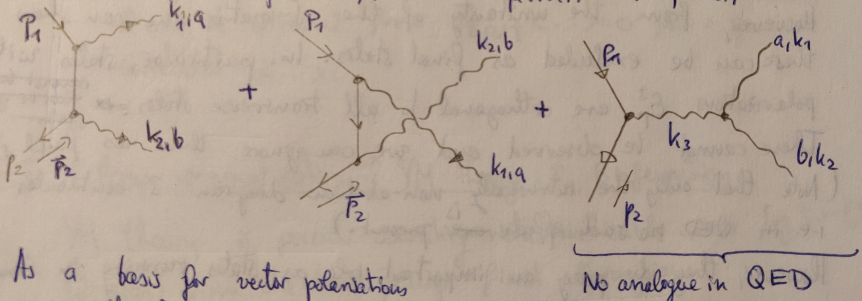
\includegraphics[width=0.7\linewidth]{gfx/YMpictures/YMfermionantifermionAnnihilation}
	\caption{Fermion and Anti-fermion annihilation processes in YM}
	\label{fig:ymfermionantifermionannihilation}
\end{figure}


As a basis for vector polarization consider the following:
\begin{equation*}
	k^2=0,\quad i.e. k^\mu = (k^0,\vec{k})\quad + \quad k^\mu\epsilon_\mu=0
\end{equation*}
satisfied for
\begin{enumerate}
	\item $\epsilon_{T,i}=(0,\vec{\epsilon}_i)^T$ with $\vec{k}\cdot\vec{\epsilon}_i$, $i=1,2,$: the transverse polarizations
	\item \begin{equation*}
		\epsilon^+ := \left(\frac{k^0}{\sqrt{2}\abs{\vec{k}}}, \frac{\vec{k}}{\sqrt{2}\abs{\vec{k}}}\right)^T\quad \text{forward light-like}.
	\end{equation*}
In addition we have 
\begin{equation*}
	\epsilon^- := \frac{1}{\sqrt{2}\abs{\vec{k}}}\left(k^0, -\vec{k}\right)^T \quad \text{backward light-like, but } k\cdot \epsilon^- \neq 0
\end{equation*}
with
\begin{align*}
	\epsilon^T_i \cdot \epsilon^T_j &= - \delta_{ij},\quad \epsilon^+\cdot \epsilon^T_i = 0 = \epsilon^- \cdot \epsilon^T_i,\\
	(\epsilon^+)^2 &=0= (\epsilon^-)^2,\quad \mI=\epsilon^+ \cdot \epsilon^-,\\
	\eta\munu &= \epsilon^-_\mu (\epsilon^+_\nu)^* + \epsilon^+_\mu (\epsilon^-_\nu)^* - \sum_{i=1,2} \epsilon^T_{i\mu} (\epsilon^T_{i\nu})^*.
\end{align*}

\end{enumerate}
Denote the amplitude by
\begin{equation}
	i M = i M^{\mu \nu} \epsilon^*_\mu(k_1) \epsilon^*_\nu(k_2)
\end{equation}
for outgoing vector polarization $\epsilon^*_\mu(k_i)$.\\
An explicit computation gives
\begin{align}
	iM^{\mu \nu} (\epsilon^T_\mu(k_1))^* (\epsilon^T_\nu(k_2 ))^* &\neq 0 \text{ both final bosons transverse}\\
	iM^{\mu \nu} (\epsilon^T_\mu(k_1))^* (\epsilon^\pm_\mu(k_2))^* &=0 \; 1 \text{ final boson null!}, \text{  but}\\
	iM^{\mu \nu} (\epsilon^+_\mu(k_1))^* (\epsilon^-_\nu(k_2))^* &\neq 0 \text{ !}
\end{align}
As in QED, the asymptotic states naively include negative norm states for time-like and zero-normstates for longitudinal polarizations. In addition, there are zero norm states in the ghost sector. However, from the unitarity of the S-matrix one can show that these can be excluded as final states. In particular, states with polarizations $\epsilon^\pm_\mu$ are orthogonal to all transverse states. These cannot be observed and we can ignore them as final states. (Note that only the intrinsically non-abelian diagram $3$ contributes to this, i.e. in QED no such effect is present.)\\
However, they do play an important role as states running loops
\begin{figure}[h!]
	\centering
	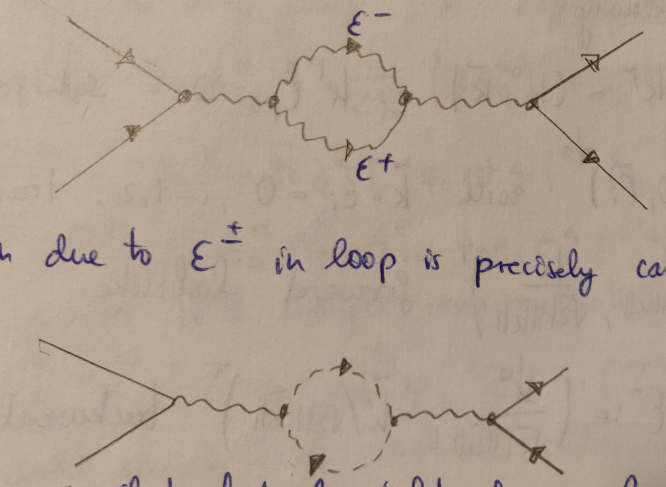
\includegraphics[width=0.7\linewidth]{gfx/YMpictures/YMghostloops}
	\caption{Ghost loops}
	\label{fig:ymghostloops}
\end{figure}


. The contribution due to $\epsilon^\pm$ in the loop is precisely cancelled by a ghost loop
if we take into account that ghost loops (like fermion loops) carry an extra factor of $(-1)$ due to their Grassmann nature.
\begin{mybox}{Ghost Fields}
	Conclusion:\\
	As advocated, ghost-fields cancel loop contributions due to unphysical vector bosons and thus serve as ’\emph{negative degrees of freedom}’.
\end{mybox}
\begin{mybox}{Slavnov-Taylor identity in YM, outlook}
	As demonstrated, in YM theory the relation
	\begin{equation}
	\label{eq:wardidQED}
		k_\mu M^\mu =0
	\end{equation}
	does in general not hold. In QED, \ref{eq:wardidQED} is a consequence of the Ward-Takahashi identity for the conserved current
	\begin{equation}
		\gamma^\mu = \bar{\psi} \gamma^\mu \psi.
	\end{equation}
	In YM, the conserved current is more complicated as it includes also $A^\mu$ itself (due to $A^3,A^4$ terms). The analogue of the Ward identities are the Slavnov-Taylor identities:\\
	Thee are the Ward Takahashi identities for $J^\mu_{BRST}$ and can be obtained from $\delta_{BRST}\expval{\dots} =0$ for a general correlator $\expval{\dots}$.
\end{mybox}
\subsubsection{Emission}

\begin{equation}
	 \feynmandiagram[horizontal=v to w]{a[particle=$\beta$] --[fermion, momentum=\(p_2\)]v --[fermion, momentum=\(p_1-k_1\)] w--[gluon, momentum=\(k_1\)] b[particle=${(a,\mu)}$], c[particle=$\alpha$]--[anti fermion, momentum=\(p_1\)] w, v--[gluon, momentum=\(k_2\)] d [particle=${(b,\nu)}$]};
\end{equation}
has the following amplitude via Feynman rules
\begin{align}
	iM&=\bar{v}^i_\alpha(p_1) i g \gamma^\mu T^a_r \epsilon^{a,\dagger}_\mu(k_1) \left(\frac{i}{\slashed{q}-m}\right)_{\alpha \beta} \delta_{ij}\epsilon^{b,*}_\nu(k_2) i g \gamma^\nu T^b_r u^j_\beta(p_2).
\end{align}
Use 
\begin{equation*}
(\slashed{p}_2-m)u(p_2)=0\quad \bar{v}(p_1) (\slashed{p}_1+m) =0, \; \mu\neq \nu \Rightarrow \; \gamma^\mu \gamma^\nu=- \gamma^\nu \gamma^\mu.
\end{equation*}
\subsubsection{Tricks in computation of scattering amplitudes}
\begin{enumerate}
	\item If computing loops with Lorentz indices, then decide which vertex (left or right) to have covariant and the other to have contravariant indices, e.g.
	\begin{equation*}
		\feynmandiagram[horizontal=v to w]{a--[gluon] v [particle=$v_1$]--[half left,gluon] w[particle=$v_2$]--[gluon]b, w--[half left, gluon] v };
	\end{equation*}
could have the following vertex structure
\begin{equation*}
	\underbrace{f^{adc} [\eta^\mu_\sigma(\dots)_\rho + \dots]}_{v_1} \underbrace{f^{bcd}[\eta^{\rho \nu} (\dots)^\sigma \dots]}_{v_2}.
\end{equation*}
\item For loop computation, only use the propagator in slimmed form as no indices/external legs present
\begin{align*}
	\feynmandiagram{a[particle=${(a,\mu)}$] --[gluon]c--[gluon] b [particle=${(b,\nu)}$]}; &= \frac{-i}{p^2+i\epsilon}\left(\eta\munu-(1-\xi) \frac{p_\mu p_\nu}{p^2}\right)\delta^{ab} \\
	\rightarrow \quad \feynmandiagram{a--[half left, gluon, edge label=$p+q$] b};&= \frac{-i}{(p+q)^2}.
\end{align*}
\item Compute the self loop
\begin{equation*}
	\feynmandiagram{a[particle=${(a,\mu)}$]--[gluon]m--[gluon, edge label=${d,\sigma}$] v--[edge label=${c,\rho}$,gluon]n--[gluon] b [particle=${(b,\nu)}$], v--[loop,min distance=2cm, gluon] v};
	\end{equation*}
as a $4$-vertex with $\sigma=\rho$ and $d=c$.
\item Trick for nasty loop integral
\begin{equation*}
	\int \frac{\md^d p}{(2 \pi)^d} \frac{1}{p^2} = \int \frac{\md^d p}{(2 \pi)^d} \underbrace{\frac{1}{p^2} \frac{1}{(p+q)^2}}_{=\frac{1}{AB}} (p+q)^2.
\end{equation*}
\item ghost loops $\Rightarrow \cdot (-1)$.
\end{enumerate}
















\subsection{Running coupling in YM}
\subsubsection{YM  $\beta$-function at $1$-loop in $g$}
As derived in \ref{subsec:renormalizationYM}, we state again the YM beta function at one-loop order \ref{eq:betafunctionYangMills}.
\begin{mybox}{YM $\beta$ function to leading order in $\md=4$}
	\begin{equation}
	\beta^{(1)}_{YM}(g) = - \frac{g^3}{(4 \pi)^2} \left[\frac{11}{3} C_2(H) - \frac{4}{3} n_f C(R_f)\right].
	\end{equation}
\end{mybox}
\subsubsection{Crucial Implications}
\begin{enumerate}
	\item \begin{mybox}{Asymptotic freedom}
	Pure non-abelian YM theory is \emph{asymptotically free} since $\beta(g)<0$ and thus $g\rightarrow 0$ as $\mu \rightarrow\infty$.
	\end{mybox}
\item \begin{mybox}{}	
	Of all known renormalizable QFTS in $D=4$, YM theory is the only one which is asymptotically free!
	Strictly speaking, it is the only one for which the UV cut-off $\Lambda$ can be taken to $\infty$ in perturbation theory.
\end{mybox}
	\item Coupling YM to fermionic matter tends to make $\beta(g)$ positive, but for sufficiently "little amount of fermions" $\beta(g)$ remains negative.
\end{enumerate}
\subsubsection{Examples}
$H=SU(N)$ with normalization 
\begin{equation}
	\tr(T^a T^b) = \half \delta^{ab} \quad \Rightarrow \quad  C_2(SU(N)) = N.
\end{equation}
Now take $n_f$ fermions in fundamental representation
\begin{equation*}
	R_f = \yng(1) \quad \text{with} \quad C\left(\yng(1)\right)=\half.
\end{equation*}
Then, the $\beta$-function of this theory at $1$-loop reads
\begin{equation}
	\beta(g) = -\frac{g^3}{(4\pi)^2} \left[\frac{11}{3} N-\frac{2}{3}n_f\right].
\end{equation}
We will use this below to find the beta function of QCD.
\subsubsection{Notes on the $\beta$ function}
Generally, to one-loop/leading order in $\lambda$, the beta function becomes
\begin{equation*}
	\beta(\lambda) = \mu \frac{\partial}{\partial \mu} \left(-\delta_{\lambda}+\frac{\lambda}{2} \sum_i \delta_{Z_i}\right)
\end{equation*}
and in non-abelian gauge theory with a renormalization scale $M$
\begin{equation*}
	\beta(g) = g M\frac{\partial}{\partial M} \left(-\delta_1+\delta_2+\frac{\delta_3}{2} \right)
\end{equation*}
which is also the $\beta(g)$ for $3$-point function $\expval{A\bar{\psi}\psi}$ at $1$-loop.
\section{Quantumchromodynamics (QCD)}
\subsection{Overview of the theory}
QCD is a $SU(3)$ YM theory
\begin{equation}
	\label{eq:qcdlagrangian}
	\mL_{QCD} = \bar{\psi}_i \left[i(i\gamma^\mu D_\mu)_{ij}-m \delta_{ij}\right]\psi_j - \frac{1}{4} F^a\munu F^{\mu \nu, a}
\end{equation}
where $\psi_i(x)$ is the quark field in the fundamental representation of the $SU(3)$ gauge group, indexed by $i,j,\dots$. The YM $SU(3)$ theory is therefore coupled to $6$ quarks in fundamental representation
\begin{equation}
q^{(f)} \equiv q^{(f)}_i,
\end{equation}
where $i=1,2,3$ are the \emph{colour indices} of the fundamental of $SU(3)$ (red,yellow,blue) and $f=1,\dots,6$ are the \emph{flavour indices} called $u,d,c$,$s,t,b$\\ The Dirac matrices $\gamma^\mu$ connect the spinor representation to the vector representation of the Lorentz group. The symbol $F^a\munu$ represents the gauge invariant gluon field strength tensor. It is given by $F^a\munu = \partial_\mu A^a_\nu$$ - \partial_\nu A^a_\mu +g f^{abc} A^b_\mu A^c_\nu$, where $A^a_\mu(x)$ are the gluon fields in the adjoint representation of the $SU(3)$ gauge group, indexed by $a,b,\dots$. The variables $m$ and $g$ correspond to the quark mass and coupling of the theory, which are subject to renormalization.\\
 Quarks are massive spin $\half$ fermions which carry a colour charge whose gauging is the context of QCD. Quarks are represented by Dirac fields in the fundamental representation of $SU(3)$. They also carry electric charge (either $-1/3$ or $2/3$) and participate in weak interactions as part of the weak Isospin doublets.\\
Gluons are spin $1$ bosons which also carry colour charges, since they lie in the adjoint representation of $SU(3)$. They have no electric charge, do not participate in the weak interactions and have no flavour.\\
QCD gives rise to three basic interactions
\begin{enumerate}
	\item A quark may emit (or absorb) a gluon,
	\item A gluon may emit (or absorb) a gluon,
	\item and two gluons may directly interact.
\end{enumerate}
This contrasts with QED, in which only the first kind of interaction occurs, since photons have no charge. Diagrams involving FP-ghosts must be considered too. Furthermore, the gluon changes the charge of the fermion, where the photon does not, which makes it more difficult to separate regimes in QCD.\\
\\
QCD is not a conformal field theory, since $\mL_{QCD}$ contains dimensionful coupling, in particular the fermionic mass $m_\psi$. This introduces a scale into the theory that makes i non-conformal. QCD($m_f=0$) is still not conformal, since massless QCD has an extra symmetry, namely \emph{Chiral symmetry}, but the coupling of the gauge potential to the fermions still needs to be renormalized, i.e. is scale-dependent.\\
The fermion-gauge field interaction temr is given by $g \bar{\psi} \gamma^\mu A_\mu \psi$ where the coupling $g$ has mass dimension zero in $D=4$ dimensions.\\
Note
\begin{equation*}
	[S]=0\Rightarrow\;[\mL_{QCD} ] = 4, [\psi]=\frac{3}{2} \& [A]=1, \; 2[\psi] + [A] = 4 \; \Rightarrow \; [g] =0
\end{equation*}
Repeating the above in other words, QCD is not conformal since it has a negative $\beta$-function 
\begin{equation}
	\beta(g) = -\frac{g^3}{(4 \pi)^2} \left[11-\frac{2}{3} n_f\right]
\end{equation}
where $n_f=6$ is the number of quark flavours. Thus,
\begin{equation}
	\beta_{QCD}(g) = -\frac{7}{16 \pi^2} g^3 \quad <0.
\end{equation}



\subsection{The theory in its full glory}
\subsubsection{Heuristic motivation of QCD Lagrangian}
Following our treatment for the general YM theory (e.g. \ref{eq:ymLagrangian}) and group theory (e.g. \ref{eq:casimir}), we 
start again heuristically with the following set-up.
\begin{enumerate}
	\item Introduce free Lagrangian for electrons $\mL_f(\psi,\partial_\mu \psi)=\bar{\psi} (i \slashed{\partial}-m) \psi$ which has an associated global $U(1)$ symmetry.
	\item Now \emph{gauge} the global symmetry, i.e. \emph{impose} local $U(1)$. This gives you problems with the derivative. In order to alleviate, we do \emph{minimal coupling}:
	\bse 
	\partial_\mu \longrightarrow D_\mu = \partial_\mu +ie Q A_\mu,
	\ese 
	where $D_\mu$ is the (gauge-)covariant derivative.
	\item Have to find the dynamics of the gauge field (photon), i.e. we add (part of the minimal coupling prescription) $\mL_A=-\frac{1}{4}F_{\mu \nu}F^{\mu \nu}$.
\end{enumerate}
Now, in order to find the Lagrangian of QCD in this way we do the following steps.
\begin{enumerate} 
	\item[Step 1]:
	What is the information that we have ?
	\begin{enumerate}
		\item Quarks are spin $\frac{1}{2}$ and come in $6$ "flavours" $q=u,d,c,s,t,b$.
		\item Quarks also have a "colour" d.o.f., i.e. we have $\psi_q = (\psi^r_q,\psi^g_q,\psi^b_g)^T$.
	\end{enumerate}
	Good starting point is the free Dirac Lagrangian
	\bse 
	\mL_q(\psi,\partial_\mu \psi) = \sum_q \bar{\psi}^i_q (i \slashed{\partial}-m_q) \delta^{ij}\psi^j_q,
	\ese 
	where $i$ indicates the colour index.
	\begin{enumerate}
		\item This has a \emph{global} $SU(N_c)$ symmetry $N_c=3$.
		\bse 
		\psi^i_q \rightarrow U_{ij}\psi^j_q \text{ where } U_{ij} =\left[\exp\left( -i g_s \theta^a t^a\right) \right]_{ij}, \; U\in SU(N_c)
		\ese 
		depends on $(N^2_C-1)$ real parameters $\theta^a$, $a=1,\dots,(N^2-1)$. The matrices $(t^a)_{ij}$ are the \emph{generators} of the \emph{fundamental} representation of $SU(N_c)$, to which $\psi_q$ belong.
		\item The properties of $t^a$ follow from $U\in SU(N_c)$ 
		\begin{enumerate}
			\item $U$ unitary 
			\bse 
			U^\dagger U = U  U^\dagger = 1 \quad \Rightarrow \quad (t^a)^\dagger = t^a,
			\ese 
			i.e. the generators are hermitian.
			\item
			\bse 
			\det(U) =1 \,  \Rightarrow \, \det(U) = \exp \left[-i g_s \Tr{t^a}\right] \, \Rightarrow\, \Tr{t^a}=0
			\ese 
			i.e. the generators are traceless.
			\item Explicit representation is given by the Gell-Mann matrices $\lambda^a$
			\bse 
			t^a = \frac{\lambda^a}{2}
			\ese 
			with common normalization being
			\bse 
			\Tr{t^a t^b} = T_F \delta^{ab},\qquad T_F = \frac{1}{2},
			\ese 
			where $T_F$ is called \emph{index} (not the Casimir) for $F$ indicating the fundamental representation.
		\end{enumerate}
	\end{enumerate}
	
	\item[Step $2$] $SU(N_c)$ is an exact symmetry, now we "gauge" it. I.e. we require invariance under \emph{local} $SU(N_c)$: $\theta^a=\theta^a(x)$. Then we have the following trafos
	\bse
	\psi(x) \rightarrow U(x) \psi(x),\; \bar{\psi}(x) \rightarrow \bar{\psi}(x) U^\dagger(x), \; U(x) = \exp \left[-i g_s \theta^a(x) t^a\right].
	\ese 
	Note that $\bar{\psi}(x) \slashed{\partial} \psi(x)$ is now not invariant any more.\\
	The covariant derivative $D_\mu$, an operator, has the property
	\bse 
	D_\mu \rightarrow D^\prime_\mu = U(x) D_\mu U^\dagger(x) \; \Rightarrow \; D_\mu \psi(x) \rightarrow U(x) D_\mu \psi 
	\ese 
	which is achieved by introducing a vector field $A^a_\mu$
	\bse 
	D_\mu \equiv \partial_\mu + i g_s \underbrace{A^a_\mu t^a}_{\mA_\mu \in M^{N_c \times N_c}}.
	\ese 
	This is the minimal coupling prescription.	
\item[Remark]
	As in our treatment of YM theory, we make this remark on the nature of the gauge covariant derivative sewing together patches of fibre bundles on which the fields live, see \ref{eq:comparator}. Therefore,  the gauge field can be understood from a geometric picture:\\
		Look at the partial derivative of an object, we see that the objects transform differently,
		\bse
		n^\mu \partial_\nu \Phi(x) = \lim_{\epsilon\rightarrow o} \frac{1}{\epsilon} \left[\underbrace{\Phi(x+\epsilon n)}_{U(x+\epsilon n)} - \underbrace{\Phi(x)}_{U(x)} \right]
		\ese 
		i.e. they live in completely different vector space. We use a transfer function (link, comparator) to transfor fields from one representation space to another
		\bse 
		W(x,y) \rightarrow U(x) W(x,y) U^\dagger(y),\quad W(x,x) \equiv 1
		\ese 
		thus the following object transforms correctly
		\bse 
		W(x+\epsilon n,x) \Phi(x) \rightarrow U(x+\epsilon n) \left[\dots\right],
		\ese 
		thus
		\bse 
		W(x+\mathrm{d}x,x) = \mI - i g_s \mA_\mu \mathrm{d}x^\mu,
		\ese 
		where $\mathcal{A}_\mu$ is a \emph{connection}. Thus, we introduce the covariant derivative as
		\be
		n^\mu D_\mu \Phi(x) = \lim_{\epsilon \rightarrow 0} \frac{1}{\epsilon} \left[\Phi(x+\epsilon n) -W(x+\epsilon n,x) \Phi(x)\right].
		\ee 
	\item[Step $3$] Now have to find dynamics of the gauge (i.e. gluon) fields
	\begin{enumerate}
		\item Generators $\hat{T}^a$ are closed under commutations, i.e. we have an algebra (Lie..)
		\bse
		[\hat{T}^a,\hat{T}^b] = i f^{abc} \hat{T}^c,
		\ese 
		where the \emph{structure constants} $f^{abc}$ encode the complete group structure. 
		\item The structure constants satisfy the Jacobi identity
		\bse 
		f^{abc} f^{cde} +f^{adc} f^{ceb} + f^{aec} f^{cbd} =0.
		\ese 
		\item The structure constants are real
		\begin{align*}  
			([t^a,t^b])^\dagger &= -i (f^{abc})^* (t^c)^\dagger = - i (f^{abc})^* t^c \\
			= [(t^a)^\dagger, (t^b)^\dagger] &= -[t^a,t^b] = -i f^{abc} t^c \Leftrightarrow f^{abc} = (f^{abc})^*.
		\end{align*} 
		\item They are totally anti-symmetric
		\begin{align*} 
			\Tr{[t^a,t^b] t^c)} &= i f^{abd} \underbrace{\Tr{t^d t^c}}_{T_F \delta^{dc}} = i T_F f^{abc} \\
			= \Tr{\left[\underbrace{t^a t^b t^c}_{t^b t^c t^a} - \underbrace{t^b t^a t^c}_{t^c t^b t^a}\right]} &= \Tr \left[\underbrace{[t^b,t^c]}_{\text{anti-symmetric}} t^a\right]
		\end{align*} 
		\item Infinitesimal global transformation 
		\begin{align*}
			A^a_\mu \rightarrow A^{\prime a}_\mu &= (\delta^{ac} + g_s \delta \theta^b f^{abc} ) A^c_\mu = (\delta^{ac} - i g_s \delta \theta^b (T^b_{(ad)})_{ac}) A^c_\mu \\
			\text{where  } (T^a_{(ad)})_{bc} &= i f^{bac} = - if^{abc},
		\end{align*}
		i.e. the generator in the \emph{adjoint} representation. Also
		\bse 
		[T^a_{(ad)} ,T^b_{(ad)}] = if^{abc} T^c_{(ad)} = \text{Jacobi identity}.
		\ese 
\footnote{ 
		People don't like that we say that gauge fields transform under adjoint rep as for a local transformation you get additional terms. Therefore, the gauge field only transform in the adjoint rep for global transformation! Alternatively look at field strength to alleviate problems.}
		\item Give \emph{dynamics} to $A^a_\mu$ by constructing the \emph{field strength}
		\bse 
		\mathcal{F}_{\mu \nu} = - \frac{i}{g_s} [D_\mu ,D_\nu ]= \partial_\mu \mA_\nu - \partial_\nu \mA_\mu + i g_S [\mA_\mu, \mA_\nu ],
		\ese \footnote{The last term is due to the fact that our gauge fields are matrices here, whereas in QED this term is zero as you have $\mC$ numbers. This term introduces self-interactions.}
		which transforms as
		\bse 
		\mF_{\mu \nu} \rightarrow \mF^\prime_{\mu \nu} = U F_{\mu \nu}  U^\dagger,
		\ese 
		such that
		\bse 
		\mF_{\mu \nu} = F^a_{\mu \nu} t^a \rightarrow F^a_{\mu \nu} = \partial_\mu A^a_\nu - \partial_\nu A^a_\mu - \underbrace{g_s f^{abc} A^b_\mu A^c_\nu }_{\text{not present in QED}}.
		\ese 
		To find a gauge and Lorenz-covariant expression built out of the field strength, we write down
		\be
		\mL_A = - \frac{1}{4 T_F} \Tr \left[ \mF_{\mu \nu} \mF^{\mu \nu}\right] - \frac{1}{4} F^a_{\mu \nu} F^{a,\mu \nu}. 
		\ee 
		This Lagrangian now has self-interactions. Similar to QED, a mass term $-m^2 A^a_\mu A^{a,\mu}$ is forbidden.
		\footnote{
		You can interpret the field strength as the curvature of the representation space where the fields live. Basically the non-vanishing $[D_\mu,D_\nu]$ is like the torsion tensor in GR, gives us a non-vanishing of two paths arriving from one point at another.}
	\todo{Insert picture}
	\end{enumerate}
	\item[Step 4] Putting it all together
	\begin{align*}
		\mL_{QCD} &= \mL_{q}|_{\partial_\mu \rightarrow D_\mu} + \mL_A = \sum_q \bar{\psi} (i \slashed{D}-m_q) \psi_q - \frac{1}{4}F^a_{\mu \nu} F^{a,\mu \nu} \\
		&=\underbrace{  \sum_q \bar{\psi}_q (i\slashed{\partial} -m_q)\psi_q - \frac{1}{4} (\partial_\mu A^a_\nu -\partial_\nu A^a_\mu) (\partial^\mu A^{a,\nu} -\partial^\mu A^{a,\nu}) }_{\text{free}} \\
		&- \underbrace{g_s t^a A^a_\mu \bar{\psi}_q \gamma^\mu \psi_q}_{\bar{q} q g} \\
		&+\underbrace{  \frac{g_s}{2} f^{abc} (\partial_\mu A^a_\nu - \partial_\nu A^a_\mu ) A^{b,\mu} A^{c,\nu}}_{\text{cubic interaction}} \\
		&- \underbrace{\frac{g^2_S}{4} f^{abc} f^{ade} A^b_\mu A^c_\nu A^{d,\mu} A^{e,\nu}}_{\text{quartic interaction}}.
	\end{align*}
	\footnote{
	One could in principle add another term to the QCD Lagrangian $
	\theta \epsilon^{\mu \nu \rho \sigma} F_{\mu \nu} F_{\rho \sigma}$
	which constitutes the \emph{strong cp problem}. This term would be connected to the neutron electric dipole moment, i.e. experimental constraints $\theta <10^{-10}$. Axion is one proposed solution to this. Nowadays one considers ALPS (axion like particles, also DM candidate (as axion)). This term can be written as a total derivative and can therefore be written as a boundary term.}
\end{enumerate}

 



\subsection{Running coupling and beta-function}
\label{subsec:qcdrunningcoupling}
Using our result for the $1$-loop YM beta function \ref{eq:betafunctionYangMills} we have
\begin{equation}
	\beta(g) = -\frac{g^3}{(4 \pi)^2} \beta_0+ \mO(g^5)
\end{equation}
with
\begin{equation}
	\beta_0=\left(\frac{11}{3}\cdot 3 - \frac{2}{3} \cdot 6\right) = 7
\end{equation}
which comes from $N=3$ for $SU(3)$ and $n_f=6$ quarks being contained in our theory.
\begin{mybox}{QCD Running Coupling}
	Note that $\alpha_s =\frac{g^2}{4 \pi}$ runs as
	\begin{equation}
		\label{eq:qcdrunningcoupling}
		\alpha_s(\mu) = \frac{\alpha_s(\mu_0)}{1 + \beta_0 \frac{\alpha_s(\mu_0)}{2 \pi} \ln(\frac{\mu}{\mu_0})}.
	\end{equation}
	Experimentally for $\mu_0\approx 91.2$ GeV (the mass of the $Z^0$-boson) we have $\alpha_s(\mu_0)\approx 0.118$.\\
\end{mybox}
\begin{mybox}{Conformal anomaly of QCD}
		Even thought QCD is conformally invariant, the non-vanishing $\beta$-function in the quantum theory means that the colour coupling needs to be renormalized and so the theory suffers from a  \emph{conformal anomaly}.
\end{mybox}
Define the strong scale $\Lambda_{QCD}$ such that at $1$ loop
\begin{equation}
	\alpha_s(\mu) \rightarrow \infty \quad \text{as} \quad \mu \stackrel{>}{\rightarrow} \Lambda_{QCD},
\end{equation}
i.e. via
\begin{equation*}
	1+\beta_0 \frac{\alpha_s(\mu_0)}{2 \pi} \ln(\frac{\Lambda_{QCD}}{\mu_0}) =0, \Leftrightarrow \; \Lambda_{QCD} \approx \mu_0 \exp \left[- \frac{1}{2 \beta_0 \frac{\alpha_s(\mu_0)}{2 \pi}}\right]
\end{equation*}
with $\Lambda_{QCD}\approx 200$MeV experimentally, where $\Lambda_{QCD}$ is called the \emph{fundamental scale of QCD} which indicates \emph{hadronization}. Then we have
\bse 
\alpha_s(\mu^2) = \frac{2 \pi}{\beta_0 \ln(\frac{\mu}{\Lambda_{QCD}} )}
\ese 
$\alpha_s$ runs as 
\begin{figure}[h!]
	\centering
	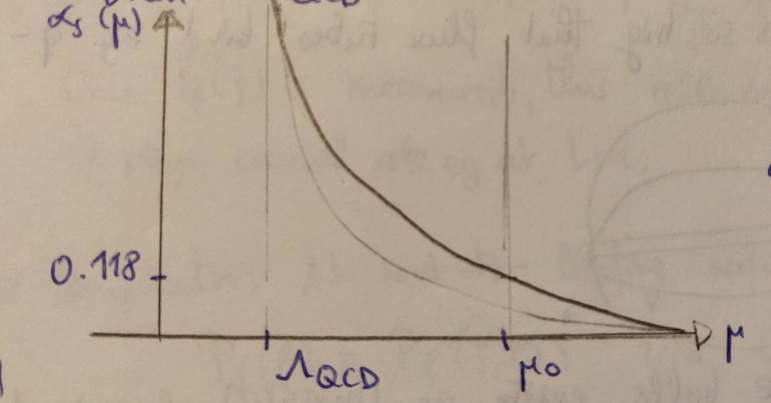
\includegraphics[width=0.7\linewidth]{gfx/YMpictures/QCDrunningcoupling}
	\caption{Running coupling of QCD}
	\label{fig:qcdrunningcoupling}
\end{figure}
according to the perturbative analysis. Note that everything below $\Lambda_{QCD}$ corresponds to \emph{confinement} and getting close to $\Lambda_{QCD}$ you should stop doing perturbation theory.
\\
Perturbation theory is valid only for processes at typical energies at $\geq 1$GeV; below that use non-perturbative methods (e.g. lattice QCD, a numerical approach to solve the path-integral due to Wilson) must be used, and they confirm that $\alpha_s$ becomes strong in the IR.
\subsection{Phase structure}
QCD exhibits an intricate phase structure, including $2$ phases:
\begin{enumerate}
\item Deconfined phase (asymptotically free):\\
For energies $\gg \Lambda_{QCD}$, QCD is weakly coupled. The observables particles are the free quarks and gluons $g^{(a)}$, $a=1,\dots,8$ ($\equiv$ QCD gauge bosons).
\item Confined phase (=\emph{hadronic phase}):\\
The observable degrees of freedom are bound states of quarks, anti-quarks and gluons, they are all given by colour singlets.\\
From
\begin{enumerate}
	\item Quarks $q_i$ in fundamental, i.e.
	\begin{equation}
		q_i \rightarrow U^{\;j}_i q_j,\quad U\in SU(3),
	\end{equation}
	and
	\item Anti-quarks $\bar{q}^i$ in anti-fundamental, i.e.
	\begin{equation}
		\bar{q}^i \rightarrow \bar{q}^j (U^\dagger)^i_{\;j},
	\end{equation}
\end{enumerate}
we can form two types of $SU(3)$ singlets
\begin{enumerate}
	\item Mesons:
	\begin{equation}
		q_i \bar{ q}^i \rightarrow q_i U^{\;j}_i (U^\dagger)^i_{\;k} \bar{q}^k = q_i \bar{q}^i,
	\end{equation}
	and
	\item Baryons:
	\begin{equation}
		\epsilon^{ijk} q_i q_j q_k \rightarrow \underbrace{(\det(U))}_{=1} \epsilon^{ijk} q_i q_j q_k.
	\end{equation}
\end{enumerate}
\end{enumerate}
The physical picture is the following:\\
QCD exhibits an intricate phase structure, including $2$ phases:
\begin{enumerate}
	\item Deconfined phase (asymptotically free):\\
	For energies $\gg \Lambda_{QCD}$, QCD is weakly coupled. The observables particles are the free quarks and gluons $g^{(a)}$, $a=1,\dots,8$ ($\equiv$ QCD gauge bosons).
	\item Confined phase (=\emph{hadronic phase}):\\
	The observable degrees of freedom are bound states of quarks, anti-quarks and gluons, they are all given by colour singlets.\\
	From
	\begin{enumerate}
		\item Quarks $q_i$ in fundamental, i.e.
		\begin{equation}
		q_i \rightarrow U^{\;j}_i q_j,\quad U\in SU(3),
		\end{equation}
		and
		\item Anti-quarks $\bar{q}^i$ in anti-fundamental, i.e.
		\begin{equation}
		\bar{q}^i \rightarrow \bar{q}^j (U^\dagger)^i_{\;j},
		\end{equation}
	\end{enumerate}
	we can form two types of $SU(3)$ singlets
	\begin{enumerate}
		\item Mesons:
		\begin{equation}
		q_i \bar{ q}^i \rightarrow q_i U^{\;j}_i (U^\dagger)^i_{\;k} \bar{q}^k = q_i \bar{q}^i,
		\end{equation}
		and
		\item Baryons:
		\begin{equation}
		\epsilon^{ijk} q_i q_j q_k \rightarrow \underbrace{(\det(U))}_{=1} \epsilon^{ijk} q_i q_j q_k.
		\end{equation}
	\end{enumerate}
\end{enumerate}
The physical picture is the following:\\
The strong force is so big that flux tubes bind e.g. $q-\bar{q}$ pairs together.



\begin{figure}[h!]
	\centering
	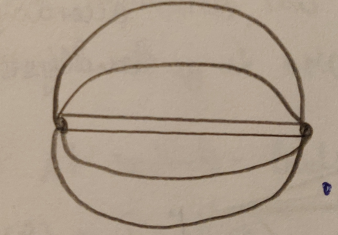
\includegraphics[width=0.7\linewidth]{gfx/YMpictures/GlueTunnel}
	\caption{}
	\label{fig:gluetunnel}
\end{figure}

In addition, glue balls exist as (mainly) gluonic bound states. To date, no analytic derivation of the hadronic spectrum starting from QCD is known.
\newpage
\subsection{Deep-inelastic scattering - Parton theory}
A useful concept for hard, i.e. high-energy scattering involving hadrons is given by the parton distribution functions:
\begin{mybox}{Parton distribution function PDF}
	Consider some hadron with momentum $P$. Then the parton-distribution function $P_F(\xi)$ is \\
	$P_f(\xi)\md \xi:=$ \emph{probability ot find a constituent $f$ ((anti-)quark or gluon) inside hadron with momentum} $p=\xi \cdot P$.
\end{mybox}
To leading order in $\alpha_s$, $P_f(\xi)$ is independent of energy scale $Q$ at which the hadron is analysed and can be determined by deep-inelastic scattering experiments of the form 

\begin{figure}[h!]
	\centering
	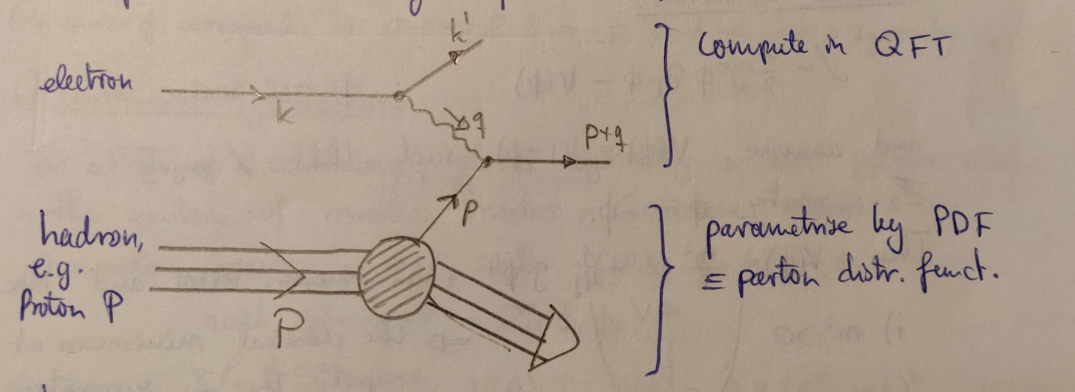
\includegraphics[width=0.7\linewidth]{gfx/YMpictures/PartonScattering}
	\caption{Parton scattering process}
	\label{fig:partonscattering}
\end{figure}










via
\begin{equation}
	\sigma(e^-(k)p(P) \rightarrow e^-(k^\prime)+X) = \int_0^1 \md \xi \sum_f P_f(\xi) \sigma\left(e^-(k) q_f( \xi p) \rightarrow e^-(k^\prime) +q_f(p^\prime)\right).
\end{equation}
Once $P_f(\xi)$ is measured, this allows for predictions for other experiments and plays a crucial role at e.g. the LHC.\\
\\
Complication:\\
At next-to-leading order, $P_f(\xi)$ is a function $P_f(\xi)\equiv P_f(\xi,Q)$ via $Q^2=-q^2$ (in above picture). I.e. at high momentum transfer, the baryon is probed at different energy scales and virtual $q-\bar{q}$ etc pairs become important ("\emph{Parton evolution}").






\subsection{Comments to think about}
\begin{enumerate}
	\item Non-abelian coupling constants are always asymptotically free. QED is abelian and has Landau pole on other side.
\end{enumerate}

\section{Standard Model of particle physics}
\label{sec:sm}
The Standard Model (SM) of particle physics is formulated as a Yang-Mills theory specified by the following data.
The gauge group of the Standard Model is 
\begin{equation}
	SU(3)_C \times SU(2)_L \times U(1)_Y.
\end{equation}
\footnote{C=\text{colour},Y=\text{Hypercharge}}
 $SU(3)_C$ describes the strong interaction, represented by QCD, with an unbroken, i.e. exact, gauge symmetry. The electroweak sector (\emph{Glashow-Weinberg-Salam} model) $SU(2)_L\times U(1)_Y$ describes electroweak interactions, i.e. two sectors which are mixed. The gauge sector of this theory is spontaneously broken to $U(1)_{QED}$ by the Higgs mechanism.\\
 \\
  The SM is a chiral theory, i.e.
 left- and righthanded fermion fields $ψ_L ≡ P_L ψ$ and $ψ_R ≡ P_R ψ$ transform in different representations. 
\\
The coupling of matter to gauge fields takes place via the covariant derivative of the SM
\begin{equation}
	D_\mu = \partial_\mu - i g_s A^a_\mu T^a_{SU(3)_C} - i g_W W^a_\mu T^a_{SU(2)_L} -i g^\prime y B_\mu,
\end{equation}
where $g_s$ is the strong coupling, $g^\prime$ the $U(1)_Y$ coupling constant, $g_W$ the $SU(2)_L$ coupling and $y$ is the hypercharge\footnote{like we have $e=Q \abs{e}$, here we do $g^\prime = g^\prime y$}. The generators are
\begin{enumerate}
	\item The one and only generator of $U(1)_Y$ is $y\mI$. Different matter fields have different values of $y$. In general due to being abelian we only know $T^{a=1}=\beta \cdot \mI$ since $[T,T]=0$, but we can choose $ T=\mI$.
	\item The generator of $SU(3)_C$ is 
	\begin{equation}
		T^a_{SU(3)_C} = \left\{ \begin{array}{ll}
		\frac{\lambda^a}{2} & \text{fundamental rep, i.e. quarks}\\
		0 & \text{singlet, i.e leptons}
		\end{array}		
		\right\}
	\end{equation}
	\item The generator of $SU(2)_L$ is 
	\begin{equation}
		T^a_{SU(2)_L} = \left\{ \begin{array}{ll}
		\frac{\sigma^a}{2}& \text{ fundamental rep., i.e. LH lepton}\\
		0 & \text{ singlet, i.e. RH lepton}
		\end{array}
		\right\}
	\end{equation}
\end{enumerate}

 
 
 
 
 
 
 
 
 
 
 
 
 
 
 The Standard Model comprises $3$ families of the following contents:
 \begin{tabular}{|l|lll|}
 	matter field          & rep. under $SU(3)_C$ & rep. under $SU(2)_L$ & rep. under $U(1)_Y=y$\\
 	\toprule
      $3\times \; Q_L$ & $\mathbf{3}$ fund. triplet eg (b,g,r)& $\mathbf{2}$ doublet & $\frac{1}{6}$\\
      $ \bar{u}_R,\bar{c}_R,\bar{t}_R$ & $\bar{\mathbf{3}}$ antifund, triplet & $\mathbf{1}$ singlet & $-\frac{2}{3}$\\
      $ \bar{d}_R, \bar{s}_R, \bar{b}_R$ & $\bar{\mathbf{3}}$ & $\mathbf{1}$& $\frac{1}{3}$ \\
  \midrule
  $e_R,\mu_R,\tau_R$ & $\mathbf{1}$ &$\mathbf{2}$ &$-\frac{1}{2}$ \\
  $\bar{ \nu}_{e,R},\bar{\nu}_{\tau,R},\bar{\nu}_{\mu,R}$ & $\mathbf{1}$ & $\mathbf{1}$ & $0$ \\
  $ \bar{e}_R,\bar{\mu}_R,\bar{\tau}_R$& $\mathbf{1}$& $\mathbf{1}$&$1$\\
  \midrule
  $H$ & $\mathbf{1}$ & $\mathbf{2}$ & $\half$\\
  \bottomrule
  $A^{QCD}_\mu$ & adjoint rep. & $\mathbf{1}$ & 0\\
  $W^{SU(2)_L}_\mu$ & $\mathbf{1}$ &adjoint rep. & 0 \\
  $B^{U(1)_Y}_\mu$ & $\mathbf{1}$& $\mathbf{1 }$& adjoint rep. \\
 \end{tabular}
where \footnote{A $0$ indicates the representation which sets everything to zero.}
\begin{enumerate}
	\item $3$ families of LH quark doublets (i.e. doublets under $SU(2)_L$)
	\begin{equation}
		Q^{i=1,2,3}_L = \begin{pmatrix}
		u^i_L\\
		d^i_L \\
		\end{pmatrix},\quad 
		\begin{pmatrix}
		c^i_L\\
		s^i_L \\
		\end{pmatrix}, \quad 
		\begin{pmatrix}
		t^i_L \\
		b^i_L \\
		\end{pmatrix},
	\end{equation}
	all of which carry a colour charge $i$ which indicates them transforming in the fundamental under $SU(3)$. 
	\item $3$ families of LH Leptons packaged as doublets under $SU(2)L$ 
	\begin{equation}
		L_L = \begin{pmatrix}
		\nu_{e_L} \\
		e_L\\
		\end{pmatrix},\quad 
		\begin{pmatrix}
		\nu_{\mu_L} \\
		\mu_L \\
		\end{pmatrix},
		\quad 
		\begin{pmatrix}
		\nu_{\tau_L} \\
		\tau_L\\
		\end{pmatrix},
	\end{equation}
	which are singlets under $SU(3)_C$, i.e. they don't carry a colour charge. We also have RH Leptons which are charged neither under $SU(3)_C$ nor $SU(2)$. Note that the RH Neutrino for all three families is absent in a minimal SM.
	\item The complex scalar Higgs field is given by a single doublet of $SU(2)_L$ 
	\begin{equation}
	H = \begin{pmatrix}
	H^+ \\
	H^0 \\
	\end{pmatrix}
	\end{equation}
	which has $4$ real degrees of freedom. We will see later that
	\begin{equation}
		\expval{H}\neq 0 \quad \Rightarrow \quad  \underbrace{SU(2)_L \times U(1)_Y}_{4 \text{ generators}}  \stackrel{SSB}{\rightarrow} \underbrace{U(1)_{QED}}_{1 \text{ generator}}
	\end{equation}
	the spontaneous breaking of $3$ generators of the electro-weak sector via the non-vanishing VEV of the SM Higgs leads to $3$ unrealized Goldstone bosons and $1$ physical Higgs. The three Goldstone bosons give rise to the longitudinal polarization of $Z^0, W^\pm$, which are massive. This is in more detail described in \ref{subsubsec:higgsSMSSB}
	\item Note that the electric charge of a particle is obtained via the sum rule
	\begin{equation}
		\label{eq:electricchargeSM}
		Q_{e} = T^3_{SU(2)_L} + y \mI_2, \quad  T^3_{SU(2)}= \left\{\begin{array}{ll}
		\begin{pmatrix}
		\underbrace{\half}_{eg. \; \nu_e} & 0 \\
		0 & \underbrace{- \half}_{eg.\; e^-} \\
		\end{pmatrix}
		& \text{if doublet }\mathbf{2}\\
		0 & \text{if singlet }\mathbf{1}\\
		\end{array}	\right\} 
	\end{equation}
\end{enumerate}

 
 
 \section{Contents of the SM}
 \subsection{Gauge fields}
 \begin{statements}
 	The number of gauge fields$=$ number of generators in Lie algebra of the corresponding gauge group.
 \end{statements}
We know that eg. $SU(N)$ has $N^2-1$ generators\footnote{Count the real degrees of freedom in a $SU(N)$ matrix, i.e. one has complex entries and thus $2 N^2$ real components, but unitarity implies $2 N^2\rightarrow N^2$ and $detU=-1$ is another condition such that $N^2-1$. }, whereas $U(1)$ has $1$ generator. 
\begin{enumerate}
	\item $SU(3)_C$ therefore has $8$ generators, which are \emph{gluons} $A^{a=1,\dots,8}_\mu$. $SU(3)_C$ is unbroken such that the gluons are massless, i.e. $m_{A^a_\mu}=0$ with $2$ spin polarizations $T_1,T_2$ or $+,-$ (where longitudinal polarization decouples due to vanishing mass.)
	\begin{statements}
		In general, any unbroken gauge theory always leads to massless gauge fields.
	\end{statements}
\item $SU(2)_L \times U(1)_Y$ has $4$ generators, i.e. $4$ gauge fields being $A^{a=1,2,3}_\mu$ for $SU(2)_L$ and $B_\mu$ for $U(1)_Y$. The SM Higgs field however breaks this gauge sector spontaneously 
\begin{equation*}
	SU(2)_L\times U(1)_Y \longrightarrow U(1)_{QED}
\end{equation*}
such that only $1$ generator is unbroken/left, i.e. the QED photon $A_\mu$. This generator is now massless but the other $3$ $W^+_\mu,W^-_\mu,Z^0$ are massive, by the Higgs mechanism, vector bosons carrying the weak interaction.
\end{enumerate}
\subsubsection{Simple Lie groups}
Consider theories invariant under $SU(N)$, which is a simple Lie group i.e. $SU(N) \neq G_1 \times G_2$. Note that $U(N)$ is a group but it is not a simple Lie group as it is isomorphic to $U(1)\times SU(N)$, which are both simple groups. \emph{Each simple group will have its own different gauge coupling} When we work with gauge theories, there is a unique coupling constant for each simple group:
\begin{align*}
	SU(2)_L& \rightarrow g_W \text{ weak coupling constant} \\
	U(1)_Y &\rightarrow g^\prime \text{ hypercharge}\\
	SU(3)_C & \rightarrow g_S \text{ strong or QED coupling}.
\end{align*}
We do not work with non-simple groups. Break groups into smallest possible decomposition of simple groups, such that we can associate a (gauge) coupling constant to each simple group.\\
To have a gauge theory, the group has to be a Lie group (i.e. a group which continuously depends on some parameters).
\begin{equation*}
	G \text{ Lie group } \Rightarrow g=\exp\left[i \sum_{a=1}^{N_G} T^a \theta^a\right] \quad \forall g\in G
\end{equation*}
where $\theta^a$ are continuous parameters and $T^a$ are the generators defining Lie group/algebra, $N_G=\#$ generators, $\{T^a\}$ satisfy the Lie algebra.
\begin{enumerate}
	\item $U(1)$ is the simplest Lie group, . Thus
	\begin{equation*}
U=e^{i\alpha}, \;\alpha \in \mR\; \forall U \in U(1 \quad \Rightarrow \;T^{a=1}=1, \theta^{a=1} = \alpha.
	\end{equation*}
\item \begin{equation*}
	U=\exp\left[i\sum_{a=1}^{N^2-1} T^a \theta^a\right]  \quad \theta^a \in \mR \forall a, U \in SU(N).
\end{equation*}
\end{enumerate}
\subsubsection{Repackaging of the gauge fields}
In fundamental representation of $SU(2)$, the generators are $T^a=\half \sigma^a$ $3$ hermitian matrices with $f^{abc} = \epsilon^{abc}$ and normalization condition
\begin{equation}
	tr(T^a T^b) =\half \delta^{ab}.
\end{equation}
A gauge field of $SU(2)$ is then introduced as
\begin{equation}
	A_\mu(x) = \sum_{a=1}^{3} g T^a \underbrace{A^a_\mu(x)}_{\text{indiv. gauge fields}},
\end{equation}
where $a$ is the \emph{Isospin index}. In gauge theory you introduce one gauge field $A_\mu(x)$ in matrix notation. It is just a convenient non-physical notation as it makes the behaviour/invariance of the triplet under gauge trafo as an invariant block easier.\\
\\
In fundamental rep of $SU(3)$, $T^{a=1,\dots,8}$ which are given by \emph{Gell-Mann} matrices $T^a =\half \lambda^a$ (all but one of them are made up of Pauli matrices, $(\lambda^a)^\dagger=\lambda^a$, 3\times 3), satisfy $[T^a,T^b] = i f^{abc} T^c$
\begin{equation*}
	A_\mu(x) =\sum_{a=1}^{8} g T^a A^a_\mu(x),\quad tr(T^a T^b) = \half \delta^{ab}.
\end{equation*}
Note that you can project this general packaging down onto a specific gluon via $tr(T^a A_\mu(x)) = \half g A^a_\mu(x)$.

\subsection{Matter fields}
\begin{enumerate}
\item The SM only contains one scalar field, the \emph{Higgs}, a complex doublet $H(x)=(H_1(x),H_2(x))^T$ (which is a doublet ito trafo under the fundamental rep of $SU(2)_L$, doesnt care about $SU(3)$). Look further for the description of the SM Higgs under \ref{subsubsec:higgsSM} and for the Higgs mechanism under \ref{subsec:higgs}.
\item All other SM matter fields are fermions.
\begin{enumerate}
	\item Consider fermions that are charged under $SU(3)_C$, i.e. quarks $q_f$ with $f=1,\dots,6$ ($f=1,\dots,N_f$ \emph{flavour index}, $N_f=\#$ flavour number)\footnote{What are the reasons for $N_f\stackrel{!}{=}6$ ? Eg. experimentally observed CP violation, apparently Neutrinos also play a role ?Apparently also $N_f$ has to be even in order to be able to form $SU(2)_L$ doublets.} (u,d,c,s,t,b). Consider one quark transforming in fundamental rep of $SU(3)_C$, i.e, it transforms as a complex triplet of $SU(3)$
	\begin{equation*}
		q_f= \begin{pmatrix}
			q^1 \\
			q^2 \\
			q^3 \\
		\end{pmatrix}
	\quad q^{1=1,2,N_c=3}_{f=1,\dots,N_f=6} \Rightarrow \; u=\begin{pmatrix}
		u^1 \\
		u^2\\
		u^3\\
	\end{pmatrix}, d=\dots
	\end{equation*}
Quarks also transform in fundamental rep under (meaning are charged under) $SU(2)_L$, i.e. they form a doublet. We can therefore combine quarks into $3$ different doublets. Only LH spinors interact with $SU(2)_L$, we thus decompose $u=(u_L,u_R)^T$ to get the $3$ \emph{families/generations}
\begin{equation*}
	\begin{pmatrix}
		u_L \\
		d_L\\
	\end{pmatrix},\quad 
\begin{pmatrix}
	c_L\\
	s_L\\
\end{pmatrix},\quad 
\begin{pmatrix}
	t_L \\
	b_L\\
\end{pmatrix},
\end{equation*}
where $u_R,d_R,\dots,b_R$ are singlets under $SU(2)_L$. Note that Parity is broken in the weak sector, i.e. group breaks into LH and RH component, where we don't observe $SU(2)_R$. The Weak sector $SU(2)_L$ breaks parity invariant maximally, charge conjugation is broken as well, but $CP$ is conserved \footnote{Apparently there is also CP non-conversation in weak sector by virtue of a mixing of the three quark generations with small angle by CabbiboKM matrix.}
\footnote{Could extend SM by $\times SU(2)_R$ "left-right symmetric models", turns out that its gauge boson would have to be way heavier than the $SU(2)_L$ ones as they have not been discovered yet.}
\item Leptons are SM fermion fields that do not transform under $SU(3)_C$ (this is the distinction between quarks and leptons, whether they participate in strong interaction):
\begin{equation*}
	e^-,\; \mu^-,\; \tau^-,\: \nu^0_e,\;, \nu^0_\mu,\; \nu^0_\tau
\end{equation*}
which are $6$ flavours of leptons $N_f=6$. We make the distinction between \emph{charged leptons} $e^-$, $\mu^-$, $\tau^-$ with $Q_{em}=-1$ and \emph{neutral leptons} $\nu^0_e$, $\nu^0_\mu$, $\nu^0_\tau$ with $Q^\nu_{em}=0$. Their LH component transforms again under fundamental rep of $SU(2)_L$, i.e. $3$ generations of doublets
\begin{equation*}
	\begin{pmatrix}
		\nu_{e,L} \\
		e_L\\
	\end{pmatrix},\quad 
\begin{pmatrix}
	\nu_{\mu,L} \\
	\mu_L\\
\end{pmatrix}, \quad 
\begin{pmatrix}
	\nu_{\tau L} \\
	\tau_L\\
\end{pmatrix},
\end{equation*}
where the RH leptons are singlets.\\
Note that $\nu_{e,R},\nu_{\mu,R},\nu_{\tau,R}$ do not transform under $SU(3)_C$, $SU(2)_L$ and $U(1)_Y$ at all. They completely decouple in the SM. In minimum SM, the RH neutrinos are not there as they do not interact at all. By oscillations and non-vanishing masses, RH neutrinos are present in SM, we ignore it in this course.
\end{enumerate} 
\end{enumerate}
\subsubsection{The SM Higgs}
\label{subsubsec:higgsSM}
The SM Higgs is a $SU(2)_L$ complex scalar doublet $H= (H^+, H^0)^T$, $H^{+,0} \in \mathbb{C}$ with the electric charge \ref{eq:electricchargeSM}
\begin{equation}
	Q_e = \left[\begin{pmatrix}
	\half &0 \\
	0 & - \half \\
	\end{pmatrix} 
	+ \begin{pmatrix}
	\half &0 \\
	0& \half \\
	\end{pmatrix}\right]
	\begin{pmatrix}
	H^+ \\
	H^0 \\
	\end{pmatrix}
	= \begin{pmatrix}
	1 & 0 \\
	0& 0 \\
	\end{pmatrix}
	\begin{pmatrix}
	H^+ \\
	H^0\\
	\end{pmatrix}.
\end{equation}
Note that we can choose unitary gauge such that \todo{how does this work, is it SU(2) or SU(4) rotation ?!}
\begin{equation}
	\expval{H} = \frac{1}{\sqrt{2}} \begin{pmatrix}
	0 \\
	v\\ 
	\end{pmatrix}, \;
	-V^{SM^classical}_{Higgs} =- \lambda (H^\dagger H - \frac{v^2}{2} )^2\; \in \mL_{SM}. 
\end{equation}
$H^+$ \footnote{Don't want to give VEV to the electrically charged field, which we could by $SU(2)$ rotation (which is globally actually broken), as it would break EM. Make sure that $v$ lives in lower component such that you can not separate electrical charges from each other by default via having a charged vacuum.}gives (in unitary gauge) rise to the longitudinal polarization of the $W^+$ boson,where the two transverse and this longitudinal polarization has been observed.\\ Experimentally we know $v\approx 246$ GeV. This VEV is the only dimensionful input paramter of the SM. All others either descend from $v$ or are dynamically generated. Eg. $\Lambda_{QCD} \approx 300$ MeV (\emph{dimensional transmutation scale of QCD} \todo{what is this ?}) is dynamiccaly generated and related to the confinement scale of QCD, it in turns implies $m_p\approx 1$ GeV $\approx m_n$.\footnote{SM would have been a scale invariant theory (CFT) if not for the experimental input of $v$. It is however not a CFT since couplings are running as $\beta \neq 0$.} This is why we say that the Higgs generates the mass spectrum of the SM (i.e. its the \emph{god particle}). In reality however, it only gives mass to quarks, $W^{\pm}$, and $Z^0$. Having found $v$ one can however generate the masses of most other particles. The baryon mass on the other hand comes from confinement.
\begin{mybox}{Hierarchy problem}
	Why is $m_{Higgs} \ll m_{pl}$ ?
\end{mybox}\todo{look into this}

















\section{Example of spontaneous symmetry breaking in QCD -- Chiral symmetry}
Consider global continuous symmetries of QCD (thus not gauge symmetry). For simplicity, we only consider the two lightest flavours $N_f =2$ and assume them to be massless $m_u=m_d=0$. Packaging them into a doublet $\begin{pmatrix}
u \\
d\\
\end{pmatrix}$, the Lagrangian is given by
\begin{equation}
	\mL= \bar{ u} (i \slashed{D} -m_u) u+ \bar{ d} (i \slashed{D} - m_d) -\underbrace{ \frac{1}{2 g^2} \tr (F\munu F^{\mu \nu})}_{\text{not relevant}} = (\bar{u}, \bar{d}) i \slashed{D} \begin{pmatrix}
	u\\
	d\\
	\end{pmatrix}.
\end{equation}
This Lagrangian exhibits two global continuous symmetries, i.e. $\mL \rightarrow \mL$ under the transformations of the symmetry group, here written as a decomposition into simple groups
\begin{equation}
	SU(2)_V\times U(1)_V \times SU(2)_A \times U(1)_A.
\end{equation}
\begin{enumerate}
	\item Vector transformation, rotates the whole Dirac fermion
	\begin{equation}
		U_V = \underbrace{e^{-i \alpha^a \half \sigma^a}}_{SU(2)_V} \cdot \underbrace{e^{-i \lambda \mI}}_{U(1)_V}, \; U_V \in SU(2)_V \times U(1)_V.
	\end{equation}
	\item Axial transformation, rotates LH and RH fermion into opposite direction
	\begin{equation}
		U_A = \underbrace{e^{-i\gamma^5 \beta^a \half \sigma^a}}_{SU(2)_A} \cdot \underbrace{e^{-i\delta \mI \gamma^5}}_{U(1)_A}, \; U_A \in SU(2)_A\times U(1)_A. 
	\end{equation}
\end{enumerate}
In reality these symmetries behave like the following
\begin{enumerate}
	\item $SU(2)_V$ is exact here, it distinguishes proton from neutron in reality. Here we have $m_u=m_d$ $\Rightarrow$ $m_p=m_n$, but as it is not exact in reality the neutron and proton have different mass.
	\item $U(1)_V$ is exact, it corresponds to the conservation of Baryon numbers, i.e. conserved charged of $B=1/3$ of $u,d$.
	\item $U(1)_A$ is anomalously broken, i.e. it is exact at the level of the classical Lagrangian level, not spontaneously broken, but it is broken by quantum corrections. We can write down Noether current for it
	\begin{equation*}
	\partial_\mu j^\mu_A = \underbrace{\text{classical level}} + j^{\mu, 5}_{\text{1 loop}} + \mO(\lambda^2).
	\end{equation*}
	Only a few expectations exist where the regularization scheme of these UV divergencies does not break the symmetry, see further Quantum anomaly or ABJ anomaly \ref{sec:anomaly}
	\item $SU(2)_A$ is spontaneously broken by the QCD vacuum, is is called \emph{Chiral symmetry of QCD}, see further \ref{subsubsec:chiralsymmetry}. \\
	Argument by SM lecturer: Have to go to confining phase (as quarks, gluons are not the correct asymptotic states of QCD) to consider mesons/baryons which are the correct asymptotic state. Experimental evidence implies that this symmetry is no there, the meson state of the theory breaks symmetry spontaneously. Symmetry has $3$ generators, thus we expect $3$ mass Goldstone bosons by the Golstone theorem, which are $\pi^{\pm,0}$, the lightest mesons of strong interaction. The mass of $\pi^{\pm,0}$ is actually non-vanishing as $u,d$ are not massless in reality, therefore the pions are called \emph{pseudo-Golstone bosons}.
	Note that the mass of the proton is set by the confining phase of QCD at $1$GeV, as symmetry of $SU(2)_A$ is spontaneously broken at this scale. Look further at dedicated section \ref{subsubsec:chiralsymmetry} for this.
 \end{enumerate}



\section{Neutrino Physics}
\subsection{Neutrino Phenomenology - Motivation to Neutrino physics}
\subsubsection{Why are neutrinos nowadays important ?}
\begin{enumerate}
	\item Neutrino masses imply physics beyond the standard model (BSM)
	\item Neutrino are the least known of SM fermions. They give a window into BSM in IR regime (even below electro-weak scale) ito. giving insight to new interactions and new particles at low energies.
	\item Neutrinos are known component of DM, but they make up HDM such that they lead to structures. Key role in the evolution of structures. AS they are HDM, they do not feel the gravitational attraction and have different contribution to CDM.
	\item Leptonic mixing, i.e. problem of flavour. We do not know why we have three generations of flavour, why is that so. Flavour structure and masses are not aligned ito. generations. Why is CP violated in leptonic sector, odd thing which we have no idea for where the reasons lie.
\end{enumerate}
\subsubsection{Open questions}
\begin{enumerate}
	\item Nature of neutrinos, could be the only Majorana particles of SM ( Neutrinoless double beta decay)
	\item Neutrino masses
	\item Neutrino mixing
\end{enumerate}
\subsubsection{Theory of Neutrinos}
As we have seen in \ref{sec:sm}, Neutrinos are packaged in $SU(2)$ doublets with hypercharge $Y=-\half$. The charge current and neutral current are then given by
\bse 
\mL = - \frac{g}{\sqrt{2}} \sum_{\alpha=e,\mu,\sigma} \bar{\nu}_{\alpha L} \gamma^\mu l_{\alpha L} W_\mu -  NC + h.c.
\ese 
where the number of active Neutrinos are
\bse 
N_\nu = \frac{\Gamma_{inv}}{\Gamma_{Z\rightarrow \nu \bar{\nu}}} = 2.984 \pm 0.008. 
\ese 

\subsection{Neutrino Oscillations}





\section{Quantum vacuum}
In quantum field theory, the quantum vacuum state (also called the quantum vacuum or vacuum state) is the quantum state with the lowest possible energy. Generally, it contains no physical particles. According to present-day understanding of what is called the vacuum state or the quantum vacuum, it is "by no means a simple empty space". According to quantum mechanics, the vacuum state is not truly empty but instead contains fleeting electromagnetic waves and particles that pop into and out of existence.\\
The QED vacuum of quantum electrodynamics (or QED) was the first vacuum of quantum field theory to be developed. \\
\\
\subsection{Quantum vacuum energy}
In many situations, the vacuum state can be defined to have zero energy, although the actual situation is considerably more subtle. The vacuum state is associated with a zero-point energy, and this zero-point energy has measurable effects. In the laboratory, it may be detected as the Casimir effect. In physical cosmology, the energy of the cosmological vacuum appears as the cosmological constant. In fact, the energy of a cubic centimeter of empty space has been calculated figuratively to be one trillionth of an erg (or $0.6$ eV). An outstanding requirement imposed on a potential Theory of Everything is that the energy of the quantum vacuum state must explain the physically observed cosmological constant.
\\
\\
Vacuum energy is an underlying background energy that exists in space throughout the entire Universe. This behaviour is codified in Heisenberg's energy–time uncertainty principle. Still, the exact effect of such fleeting bits of energy is difficult to quantify. The vacuum energy is a special case of zero-point energy that relates to the quantum vacuum.\\
The effects of vacuum energy can be experimentally observed in various phenomena such as spontaneous emission, the Casimir effect and the Lamb shift, and are thought to influence the behavior of the Universe on cosmological scales. Using the upper limit of the cosmological constant, the vacuum energy of free space has been estimated to be $10^{-9}$ joules $(10^{−2} ergs)$ per cubic meter. However, in both quantum electrodynamics (QED) and stochastic electrodynamics (SED), consistency with the principle of Lorentz covariance and with the magnitude of the Planck constant suggest a much larger value of $10^{113}$ joules per cubic meter. This huge discrepancy is known as the \emph{cosmological constant problem}.
\begin{mybox}{Cosmological constant problem}
	Why does the zero-point energy of the vacuum not cause a large cosmological constant? What cancels it out?
\end{mybox}
The theory considers vacuum to implicitly have the same properties as a particle, such as spin or polarization in the case of light, energy, and so on. According to the theory, most of these properties cancel out on average leaving the vacuum empty in the literal sense of the word. One important exception, however, is the vacuum energy or the vacuum expectation value of the energy. The quantization of a simple harmonic oscillator requires the lowest possible energy, or zero-point energy of such an oscillator to be:
\begin{equation}
E=\half h \nu.
\end{equation}
Summing over all possible oscillators at all points in space gives an infinite quantity. To remove this infinity, one may argue that only differences in energy are physically measurable, much as the concept of potential energy has been treated in classical mechanics for centuries. This argument is the underpinning of the theory of renormalization. In all practical calculations, this is how the infinity is handled.\\
Vacuum energy can also be thought of in terms of virtual particles (also known as vacuum fluctuations) which are created and destroyed out of the vacuum. These particles are always created out of the vacuum in particle–antiparticle pairs, which in most cases shortly annihilate each other and disappear. However, these particles and antiparticles may interact with others before disappearing, a process which can be mapped using Feynman diagrams. Note that this method of computing vacuum energy is mathematically equivalent to having a quantum harmonic oscillator at each point and, therefore, suffers the same renormalization problems.\\
Additional contributions to the vacuum energy come from spontaneous symmetry breaking in quantum field theory.
\subsubsection{Implications}
\begin{enumerate}
	\item Vacuum energy has a number of consequences. In 1948, Dutch physicists Hendrik B. G. Casimir and Dirk Polder predicted the existence of a tiny attractive force between closely placed metal plates due to resonances in the vacuum energy in the space between them. This is now known as the Casimir effect and has since been extensively experimentally verified. It is therefore believed that the vacuum energy is "real" in the same sense that more familiar conceptual objects such as electrons, magnetic fields, etc., are real. However, alternative explanations for the Casimir effect have since been proposed
	\item Other predictions are harder to verify. Vacuum fluctuations are always created as particle–antiparticle pairs. The creation of these virtual particles near the event horizon of a black hole has been hypothesized by physicist Stephen Hawking to be a mechanism for the eventual "evaporation" of black holes. If one of the pair is pulled into the black hole before this, then the other particle becomes "real" and energy/mass is essentially radiated into space from the black hole. This loss is cumulative and could result in the black hole's disappearance over time. The time required is dependent on the mass of the black hole (the equations indicate that the smaller the black hole, the more rapidly it evaporates) but could be on the order of $10^{100}$ years for large solar-mass black holes.
	\item The vacuum energy also has important consequences for physical cosmology. General relativity predicts that energy is equivalent to mass, and therefore, if the vacuum energy is "really there", it should exert a gravitational force. Essentially, a non-zero vacuum energy is expected to contribute to the cosmological constant, which affects the expansion of the universe. In the special case of vacuum energy, general relativity stipulates that the gravitational field is proportional to $ρ + 3p$. Quantum theory of the vacuum further stipulates that the pressure of the zero-state vacuum energy is always negative and equal in magnitude to $ρ$. Thus, the total is $ρ + 3p = ρ − 3ρ = −2ρ$, a negative value. If indeed the vacuum ground state has non-zero energy, the calculation implies a repulsive gravitational field, giving rise to acceleration of the expansion of the universe,. However, the vacuum energy is mathematically infinite without renormalization, which is based on the assumption that we can only measure energy in a relative sense, which is not true if we can observe it indirectly via the cosmological constant.
\end{enumerate}
\subsection{Symmetry}
For a relativistic field theory, the vacuum is Poincaré invariant, which follows from Wightman axioms but can be also proved directly without these axioms. Poincaré invariance implies that only scalar combinations of field operators have non-vanishing VEV's. The VEV may break some of the internal symmetries of the Lagrangian of the field theory. In this case the vacuum has less symmetry than the theory allows, and one says that spontaneous symmetry breaking has occurred. See Higgs mechanism, standard model.
\subsection{Vacuum expectation value}
If the quantum field theory can be accurately described through perturbation theory, then the properties of the vacuum are analogous to the properties of the ground state of a quantum mechanical harmonic oscillator, or more accurately, the ground state of a measurement problem. In this case the vacuum expectation value (VEV) of any field operator vanishes. For quantum field theories in which perturbation theory breaks down at low energies (for example, Quantum chromodynamics or the BCS theory of superconductivity) field operators may have non-vanishing vacuum expectation values called condensates. In the Standard Model, the non-zero vacuum expectation value of the Higgs field, arising from spontaneous symmetry breaking, is the mechanism by which the other fields in the theory acquire mass.\\
In quantum field theory the vacuum expectation value (also called condensate or simply VEV) of an operator is its average, expected value in the vacuum. The vacuum expectation value of an operator $\mO$ is usually denoted by $\expval{\mO}$. One of the most widely used examples of an observable physical effect that results from the vacuum expectation value of an operator is the Casimir effect.\todo{Link problem set from QFT I here for casimir effect}\\
This concept is important for working with correlation functions in quantum field theory. It is also important in spontaneous symmetry breaking. Examples are:
\begin{enumerate}
	\item The Higgs field has a vacuum expectation value of $246$ GeV This non-zero value underlies the Higgs mechanism of the Standard Model. This value is given by $v=\frac{1}{\sqrt {{\sqrt {2}}G^{0}_{F}}}=2\frac{M_{W}}{g}\approx 246.22$ GeV, where $M_W$ is the mass of the $W$ Boson,$G^{0}_F$ the reduced Fermi constant, and $g$ the weak isospin coupling, in natural units.
	\item The chiral condensate in Quantum chromodynamics, about a factor of a thousand smaller than the above, gives a large effective mass to quarks, and distinguishes between phases of quark matter. This underlies the bulk of the mass of most hadrons.
	\item The gluon condensate in Quantum chromodynamics may also be partly responsible for masses of hadrons.
\end{enumerate}
The observed Lorentz invariance of space-time allows only the formation of condensates which are Lorentz scalars and have vanishing charge. Thus fermion condensates must be of the form $\expval{\bar{ \psi}\psi}$,where $\psi$ is the fermion field. Similarly a tensor field, $G\munu$, can only have a scalar expectation value such as $\expval{G\munu G^{\mu \nu}}$.\\
In some vacua of string theory, however, non-scalar condensates are found. If these describe our universe, then Lorentz symmetry violation may be observable.

\subsection{Wightman Axioms}
\todo{Look into Wightman Axioms wikipedia, many interesting implication}
Axiomatic QFT says that a QFT has to have a unique vacuum.
\subsection{QCD vacuum}
The QCD vacuum is the vacuum state of quantum chromodynamics (QCD). It is an example of a non-perturbative vacuum state, characterized by non-vanishing condensates such as the gluon condensate and the quark condensate in the complete theory which includes quarks. The presence of these condensates characterizes the confined phase of quark matter.
\subsubsection{Symmetries and symmetry breaking}
Symmetries of the QCD Lagrangian:\\
Like any relativistic quantum field theory, QCD enjoys Poincaré symmetry including the discrete symmetries CPT (each of which is realized). Apart from these space-time symmetries, it also has internal symmetries. Since QCD is an $SU(3)$ gauge theory, it has local $SU(3)$ gauge symmetry.\\
Since it has many flavours of quarks, it has approximate flavour and chiral symmetry. This approximation is said to involve the chiral limit of QCD. Of these chiral symmetries, the baryon number symmetry is exact. Some of the broken symmetries include the axial $U(1)$ symmetry of the flavour group. This is broken by the chiral anomaly, cf. \ref{subsubsec:chiralsymmetry}. The presence of instantons implied by this anomaly also breaks CP symmetry.\\
In summary, the QCD Lagrangian has the following symmetries:
\begin{enumerate}
	\item Poincaré symmetry and CPT (also each one respectively) invariance
	\item $SU(3)$ local gauge symmetry
	\item Approximate global $SU(N_f) \times SU(N_f)$ flavour chiral symmetry and the $U(1)$ baryon number symmetry

\end{enumerate}
	The following classical symmetries are broken in the QCD Lagrangian:
	\begin{enumerate}
		\item scale, i.e., conformal symmetry (through the scale anomaly), giving rise to asymptotic freedom
		\item the axial part of the $U(1)$ flavour chiral symmetry (through the chiral anomaly), giving rise to the strong CP problem.
	\end{enumerate}

Symmetries of the QCD vacuum:\\
The $SU(N_f) \times SU(N_f)$ chiral flavour symmetry of the QCD Lagrangian is broken in the vacuum state of the theory. The symmetry of the vacuum state is the diagonal $SU(N_f)$ part of the chiral group. The diagnostic for this is the formation of a non-vanishing chiral condensate $\expval{\psi_i\psi_i}$, where $\psi_i$ is the quark field operator, and the flavour index $i$ is summed. The Goldstone bosons of the symmetry breaking are the pseudoscalar mesons.\\
When $Nf = 2$, i.e., only the up and down quarks are treated as massless, the three pions are the Goldstone bosons. When the strange quark is also treated as massless, i.e., $Nf = 3$, all eight pseudoscalar mesons of the quark model become Goldstone bosons. The actual masses of these mesons are obtained in chiral perturbation theory through an expansion in the (small) actual masses of the quarks. Experimentally it is seen that the masses of the octet of pseudoscalar mesons is very much lighter than the next lightest states; i.e., the octet of vector mesons (such as the rho meson). The most convincing evidence for SSB of the chiral flavour symmetry of QCD is the appearance of these pseudo-Goldstone bosons. These would have been strictly massless in the chiral limit. There is convincing demonstration that the observed masses are compatible with chiral perturbation theory. The internal consistency of this argument is further checked by lattice QCD computations which allow one to vary the quark mass and check that the variation of the pseudoscalar masses with the quark mass is as required by chiral perturbation theory.\\
In other phases of quark matter the full chiral flavour symmetry may be recovered, or broken in completely different ways.














\subsection{QED vacuum}
\todo{all of these on Wikipedai}
\subsection{Zero-point energy}


\subsection{Virtual particle}
\subsection{Quantum fluctuations}

















\section{Spontaneous symmetry breaking}
\label{sec:spontaneoussymmetrybraking}
Spontaneous symmetry breaking is a spontaneous process of symmetry breaking, by which a physical system in a symmetric state ends up in an asymmetric state. In particular, it can describe systems where the equations of motion or the Lagrangian obey symmetries, but the lowest-energy vacuum solutions do not exhibit that same symmetry. When the system goes to one of those vacuum solutions, the symmetry is broken for perturbations around that vacuum even though the entire Lagrangian retains that symmetry. SSB therefore occurs when a physical theory has some symmetry, but the \emph{ground state is degenerate} and a particular choice of vacuum does not respect this symmetry.\\
It is a universal phenomenon in physics, eg. 
\begin{enumerate}
	\item In condensed matter: ferromagnetism by alignment of atomic spins, superconductivity.
	\item In QFT: Higgs Sector of SM, chiral symmetry breaking in QCD.
\end{enumerate}
Consider a symmetric upward dome with a trough circling the bottom, i.e. Mexican hat potential. If a ball is put at the very peak of the dome, the system is symmetric with respect to a rotation around the center axis. But the ball may spontaneously break this symmetry by rolling down the dome into the trough, a point of lowest energy. Afterwards, the ball has come to a rest at some fixed point on the perimeter. The dome and the ball retain their individual symmetry, but the system does not.\\
n the simplest idealized relativistic model, the spontaneously broken symmetry is summarized through an illustrative scalar field theory. The relevant Lagrangian of a scalar field $\phi$, which essentially dictates how a system behaves, can be split up into kinetic and potential terms,
\begin{equation}
	\mL = \partial^\mu \phi \partial_\mu \phi - V(\phi).
\end{equation}
It is in this potential term $V(\phi)$ that the symmetry breaking is triggered. An example of a potential, due to Jeffrey Goldstone is illustrated by the "Mexican hat potential".
\begin{equation}
	V=\lambda ( \abs{\phi}^2 - v^2)^2
\end{equation}
with $v = \expval{\phi}$ the vacuum expectation value (vev). You can plot the "Mexican hat potential" out by decomposing $\phi=\phi_1 + i \phi_2$ with $\phi_{1,2}$ being real scalar fields.
This potential has an infinite number of possible minima (vacuum states) given by
\begin{equation}
\phi = v e^{i \xi} ,\quad \xi \in [0,2\pi].
\end{equation}
The system also has an unstable vacuum state corresponding to $\phi = 0$. This state has a $U(1)$ symmetry. However, once the system falls into a specific stable vacuum state (amounting to a choice of $\xi$), this symmetry will appear to be lost, or "spontaneously broken".
\\
In fact, any other choice of $\xi$ would have exactly the same energy, implying the existence of a massless Nambu–Goldstone boson, the mode running around the circle at the minimum of this potential, and indicating there is some memory of the original symmetry in the Lagrangian.\\
Whilst the Lagrangian is symmetric under global $U(1)$ transformation, the full quantum theory is not (this is called dynamical symmetry breaking, see below).  This is because we have t choose the vacuum state of the theory, i.e. the vacuum is not unique and we have to pick one. The Hilbert space of particle states is therefore not invariant anymore.
\subsection{Discrete Symmetries}
Consider a real scalar theory
\begin{equation*}
	\mL = \half \partial^\mu \phi \partial_\mu \phi - V(\phi)
\end{equation*}
and assume $V(\phi)=V(-\phi)$, such that $\mL$ enjoys a $\mathbb{Z}_2$-symmetry $\phi \rightarrow -\phi$.\\
Then we assume
\begin{equation*}
	V(\phi) = \half m^2 \phi^2 + \frac{1}{4!} g \phi^4 + \text{ non-renorm. terms}
\end{equation*}
and take $g>0$. Consider the two distinct case as depicted in \ref{fig:ssb}
\begin{figure}[h!]
	\centering
	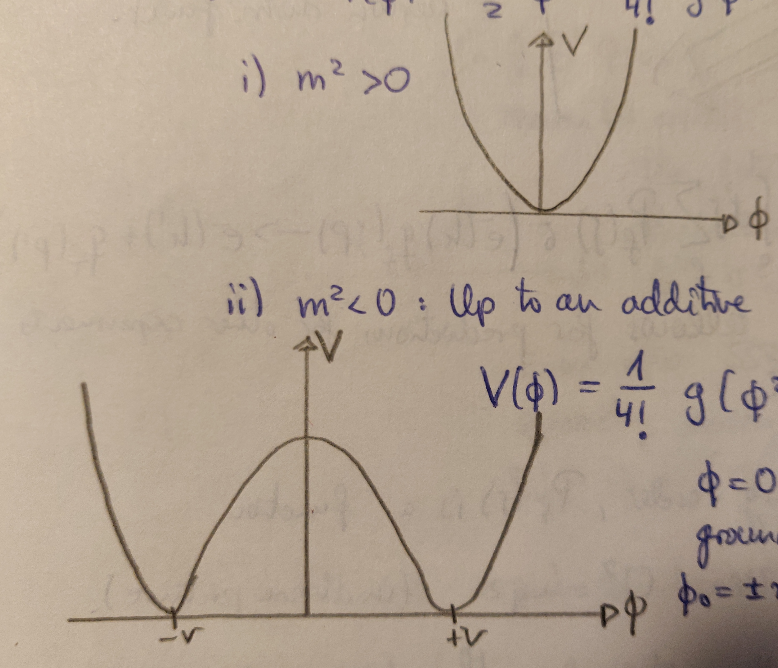
\includegraphics[width=0.7\linewidth]{gfx/YMpictures/SSB}
	\caption{}
	\label{fig:ssb}
\end{figure}
\begin{enumerate}
	\item $m^2>0$, compare \ref{fig:ssb}. We find the classical minimum at $\phi_0=0$ which respects the $\mathbb{Z}_2$ symmetry.
	\item $m^2<0$: Up to an additive constant, we can rewrite the potential as
	\begin{equation}
	V(\phi) = \frac{1}{4!} g(\phi^2- v^2)^2
	\end{equation}
	from which we can read off that $\phi=0$ is not a ground state. The classical ground state at $\phi_0=\pm v$ is degenerate. If $\phi_0=\pm v$, then the symmetry is \emph{broken}.
\end{enumerate}
In QFT, we define the excitations around that vacuum, e.g. $\phi_0=+ v$ by making a mean field approach 
\begin{equation}
	\phi=v+f
\end{equation}
and rewriting $\mL$ as 
\begin{equation}
	\label{eq:ssbLagrangian}
	\mL = \half \partial_\mu f \partial^\mu f - \frac{1}{6} g \left[ v^2 \cdot f^2+ v\cdot f^3 + \frac{1}{4} f^4\right].
\end{equation}
This looks like the theory of a massive scalar $f$ with 
\begin{equation}
	m f^2 = \frac{g}{3} v^3.
\end{equation}
The classical vacuum is at $f=0$ (i.e. at $\phi=v$). \\
\\
We now expand $\hat{f}(x)$ in quantum theory into creation/annihilation modes and  define particles in this way as excitations of $\hat{f}$, i.e. as excitations of $\hat{\phi} = v+ \hat{f}$ around $\expval{\hat{ \phi}}=v$.\\
Note: $f(x)$ has no $\mathbb{Z}_2$-symmetry left, the theory is \emph{spontaneously broken}\footnote{As $\phi\rightarrow -\phi$ corresponds to $v\rightarrow -v$ and $f \rightarrow - f$ and not just a symmetry of $f$ above.}.
\subsection{Continuous symmetries}
For SSb of a continuous, global symmetry a new feature occurs:\\
the existence of massless modes = \emph{Goldstone modes}.\\
\\
Example:\\
Consider a real scalar field $\phi=(\phi_1,\dots,\phi_n)^T$ with $\phi^2 = \phi \circ \phi = \sum_r \phi_r \phi_r$ and
\begin{equation}
\mL = \half \partial^\mu \phi \partial_\mu \phi - V(\phi), \quad V(\phi)= \frac{1}{8} g (\phi^2-v^2)^2, \quad g>0.
\end{equation}
This potential is what people generally (questionable choice of name) call the \emph{Mexican hat potential}, see \ref{fig:mexicanhatpotential}.
\begin{figure}[h!]
	\centering
	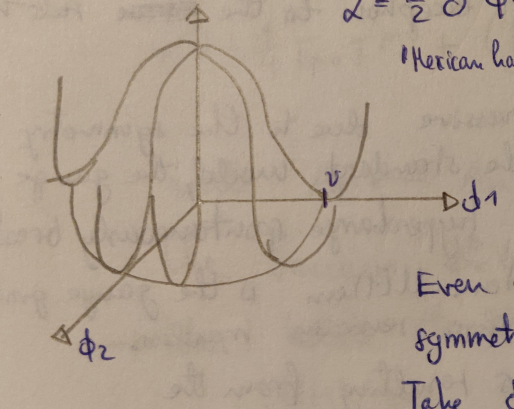
\includegraphics[width=0.7\linewidth]{gfx/YMpictures/MexicanHatPotential}
	\caption{}
	\label{fig:mexicanhatpotential}
\end{figure}
The full symmetry group of $V$ is $G=O(n)$ with the classical ground state being $\phi=\phi_0$ such that $\phi^2_0=v^2$.\\
Even after SSB, i.e. in the vacuum $\phi_0$, there is a residual symmetry corresponding to remaining flat directions:\\
Take $\phi_0=(\underbrace{0,\dots,0}_{(n-1)}, v) \Rightarrow$ $\phi_0$ is invariant under $H=O(n-1)$.\\
\\
Expand $\phi$ about a choice of vacuum $\phi_0$ as above:
\begin{align*}
	\phi&= (\phi_\perp, v+f),\quad \phi_\perp = (\phi_1,\dots,\phi_{n-1}) \\
	V(\phi)&= \frac{g}{2} v^2 f^2 + \frac{g}{2} v (\phi^2_\perp + f^2)f+ \frac{1}{8} g (\phi^2_\perp +f^2)^2.
\end{align*}
From this we can read off
\begin{equation*}
	\begin{array}{ll}
		f \text{ is massive }m^2_f=g v^2 \; &\Rightarrow \; 1 \text{ massive field (e.g. Higgs)}\\
		\phi_\perp \text{ has no mass-term } &\Rightarrow (n-1) \text{ massless fields}\\
	\end{array}
\end{equation*}
The massless fields are called \emph{Goldstone modes} or \emph{Goldstone bosons}.
\subsubsection{What is the idea behind this ?}
We obtain light or massless scalars in the full quantum theory through SSB. The minimum of this potential $V(\phi)$, i.e. the vacuum lies not at the origin but rather degenerates to lie anywhere on the sphere $\mathbb{S}^{n-1}$ defined by $\expval{\phi}=v$. Even if a universe described by such a theory would start at $\phi=0$, quantum fluctuations would quickly destabilize it, leading the whole universe to decay into one of its true  vacuum configurations on $\mathbb{S}^{n-1}$. In that configuration, there would now be one direction in field configuration space, namely the one orthogonal to the sphere, in which the potential $V(\phi)$ has non-zero curvature giving rise to a massive scalar. The Higgs field is an example of this.\\
In all other $n-1$ dimensions, the potential is constant, yielding $n-1$ Goldstone bosons.\\
These Goldstone bosons are massless scalars in the full quantum theory and therefore \textbf{pose an exception to the rule that scalars should be heavy}.
 \paragraph{Example}
The $W^{\pm}$ and $Z^0$ bosons are massive due to the symmetry breaking mechanism. In the SM, the gauge group of the weak force and spontaneously breaks to $SU(2)\times U(1)_Y$$\rightarrow U(1)_{QED}$. $U(1)_{QED}$ is the gauge group of the photon which therefore remains massless. The three Goldstone bosons resulting from the disappearance of $SU(2)$ lend mass to $W^{\pm}$ and $Z^0$.

\subsubsection{The Goldstone Theorem}
For a more in depth treatment look at \ref{subsec:goldstone}.\\
\begin{mybox}{Goldstone's theorem}
	Given a quantum theory with SSB from $G$ to $H$ as above, then there exist 
	\begin{equation*}
		(\dim G-\dim H) \text{ zero mass scalars } = \text{ Goldstone bosons}.
	\end{equation*}
\end{mybox}
Suppose $V$ has global, continuous symmetry $G$ and the vacuum breaks $G\rightarrow H$ spontaneously. Then, the theory after symmetry breaking shows
\begin{equation*}
	(\dim G-\dim H) \text{ massless scalars } = \text{ Goldstone bosons }.
\end{equation*}
\subsection{Goldstone theorem}
\label{subsec:goldstone}
In particle and condensed matter physics, Goldstone bosons or Nambu–Goldstone bosons (NGBs) are bosons that appear necessarily in models exhibiting spontaneous breakdown of continuous symmetries.
\begin{mybox}{Goldstone theorem}
	Goldstone's theorem examines a generic continuous (global) symmetry of the Lagrangian which is spontaneously broken; i.e., its currents are conserved, but the ground state is not invariant under the action of the corresponding charges. Then, necessarily, new massless (or light, if the symmetry is not exact) scalar particles appear in the spectrum of possible excitations. There is one scalar particle—called a Nambu–Goldstone boson—for each generator of the symmetry that is broken, i.e., that does not preserve the ground state. The Nambu–Goldstone mode is a long-wavelength fluctuation of the corresponding order parameter.\\
	In theories with gauge symmetry, i.e. with local continuous symmetries, the Goldstone bosons are "eaten" by the gauge bosons. The latter become massive and their new, longitudinal polarization is provided by the Goldstone boson.
\end{mybox}
Some intuition why the Goldstone boson should be massless in the case of explicit calculation of spontaneous symmetry breaking ;\\
If you split the potential into contributions from real fields $\phi_1$, $\phi_2$, we observe that the minima of the potential make up a circle in the $(\phi_1,\phi_2)$-plane. However, the potential only increases in $\phi_1$ direction, therefore moving a bit in $\phi_2$ direction does not require any energy to climb up the potential for the fluctuations to take place, therefore $m_{\rho_2}=0$ and we only find massless modes in this field-axis.\\

\subsubsection{Explicit calculation}
Consider a complex scalar field $\phi$, with the constraint that $\phi^* \phi=v^2$, a constant. One way to impose a constraint of this sort is by including a potential interaction term in its Lagrangian density,
\begin{equation}
V(\phi) = \lambda (\phi^* \phi - v^2)^2,
\end{equation}
and taking the limit as $\lambda \rightarrow \infty$  (this is called the "\emph{Abelian nonlinear $\sigma$-model}". It corresponds to the Goldstone sombrero potential where the tip and the sides shoot to infinity, preserving the location of the minimum at its base).\\
The constraint, and the action, below, are invariant under a $U(1)$ phase transformation, $\delta \phi = i \epsilon \phi$. The field can be redefined to give a real scalar field (i.e., a spin-zero particle) $\theta$ without any constraint by
\begin{equation}
\phi = v e^{i \theta}
\end{equation}
where $\theta$ is the Nambu–Goldstone boson (actually $v\theta$ is), and the $U(1)$ symmetry transformation effects a shift on $\theta$, namely
\begin{equation}
\delta \theta = \epsilon
\end{equation}
but does not preserve the ground state $\ket{0}$ (i.e. the above infinitesimal transformation does not annihilate it—the hallmark of invariance), as evident in the charge of the current below.\\
Thus, the vacuum is degenerate and noninvariant under the action of the spontaneously broken symmetry.\\
The corresponding Lagrangian density is given by
\begin{equation}
\mL =- \half \partial^\mu \phi^* \partial_\mu \phi + m^2 \phi^* \phi = -\half \left(-i ve^{-i \theta} \partial^\mu \theta\right)\left(ive^{i\theta} \partial_\mu \theta\right) + m^2 v^2
\end{equation}
and thus
\begin{equation}
= -\frac{v^2}{2} \partial^\mu \theta\partial_\mu\theta + m^2 v^2.
\end{equation}
Note that the constant term $m^2v^2$ in the Lagrangian density has no physical significance, and the other term in it is simply the kinetic term for a massless scalar.
\\
The symmetry-induced conserved $U(1)$ current is
\begin{equation}
J_\mu = -v^2 \partial_\mu \theta.
\end{equation}
The charge, $Q$, resulting from this current shifts $\theta$ and the ground state to a new, degenerate, ground state. Thus, a vacuum with $\expval{\theta}=0$ will shift to a different vacuum with $\expval{\theta}=-\epsilon$. The current connects the original vacuum with the Nambu–Goldstone boson state, $\expval{J_0(0)}{0} \neq 0$.\\
In general, in a theory with several scalar fields, $\phi_j$, the Nambu–Goldstone mode $\phi_g$ is massless, and parameterises the curve of possible (degenerate) vacuum states. Its hallmark under the broken symmetry transformation is nonvanishing vacuum expectation $\expval{\delta \phi_g}$, an order parameter, for vanishing $\expval{\phi_g}=0$, at some ground state $\ket{0}$ chosen at the minimum of the potential, $\expval{\frac{\partial V}{\partial \phi_i}}=0$. Symmetry dictates that all variations of the potential with respect to the fields in all symmetry directions vanish. The vacuum value of the first order variation in any direction vanishes as just seen; while the vacuum value of the second order variation must also vanish, as follows. Vanishing vacuum values of field symmetry transformation increments add no new information.\\
By contrast, however, nonvanishing vacuum expectations of transformation increments, $\expval{\delta \phi_g}$, specify the relevant (Goldstone) null eigenvectors of the mass matrix,
\begin{equation}
\expval{\frac{\partial^2 V}{\partial \phi_i \partial_j}} \expval{\delta \phi_g} =0
\end{equation}
and hence the corresponding zero-mass eigenvalues.
\subsubsection{Goldstone's argument}
The principle behind Goldstone's argument is that the ground state is not unique. Normally, by current conservation, the charge operator for any symmetry current is time-independent,
\begin{equation}
\frac{\md Q}{\md t} = \int \md x J^0(x) = 0.
\end{equation}
Acting with the charge operator on the vacuum either annihilates the vacuum, if that is symmetric; else, if not, as is the case in spontaneous symmetry breaking, it produces a zero-frequency state out of it, through its shift transformation feature illustrated above. Actually, here, the charge itself is ill-defined, cf. the Fabri–Picasso argument below.\\
But its better behaved commutators with fields, that is, the nonvanishing transformation shifts $\expval{\delta \phi_g}$, are, nevertheless, time-invariant,
\begin{equation}
\frac{\md \expval{\delta \phi_g}}{\md t} = 0
\end{equation}
thus generating a $\delta(k^0)$ in its Fourier transform. (This ensures that, inserting a complete set of intermediate states in a nonvanishing current commutator can lead to vanishing time-evolution only when one or more of these states is massless.)\\
Thus, if the vacuum is not invariant under the symmetry, action of the charge operator produces a state which is different from the vacuum chosen, but which has zero frequency. This is a long-wavelength oscillation of a field which is nearly stationary: there are physical states with zero frequency, $k^0$, so that the theory \textbf{cannot have a mass gap}. However this argument fails when the symmetry is gauged, because then the symmetry generator is only performing a gauge transformation. A gauge transformed state is the same exact state, so that acting with a symmetry generator does not get one out of the vacuum.
\subsubsection{Non-relativistic theories}
A version of Goldstone's theorem also applies to nonrelativistic theories (and also relativistic theories with spontaneously broken spacetime symmetries, such as Lorentz symmetry or conformal symmetry, rotational, or translational invariance).\\
It essentially states that, for each spontaneously broken symmetry, there corresponds some quasiparticle with no energy gap—the nonrelativistic version of the mass gap. (Note that the energy here is really $H−\mu N−\vec{\alpha}\cdot \vec{P}$ and not $H$.) However, two different spontaneously broken generators may now give rise to the same Nambu–Goldstone boson. For example, in a superfluid, both the $U(1)$ particle number symmetry and Galilean symmetry are spontaneously broken. However, the phonon is the Goldstone boson for both.\\
In general, the phonon is effectively the Nambu–Goldstone boson for spontaneously broken Galilean/Lorentz symmetry. However, in contrast to the case of internal symmetry breaking, when spacetime symmetries are broken, the order parameter need not be a scalar field, but may be a tensor field, and the corresponding independent massless modes may now be fewer than the number of spontaneously broken generators, because the Goldstone modes may now be linearly dependent among themselves: e.g., the Goldstone modes for some generators might be expressed as gradients of Goldstone modes for other broken generators.
\subsubsection{Pseudo-Goldstone bosons}
Pseudo-Goldstone bosons arise in a quantum field theory with both spontaneous and explicit symmetry breaking. These two types of symmetry breaking typically occur separately, and at different energy scales, and are not thought to be predicated on each other.
In the absence of explicit breaking, spontaneous symmetry breaking would engender massless Nambu–Goldstone bosons for the exact spontaneously broken chiral symmetries. The chiral symmetries discussed, however, are only approximate symmetries, given their small explicit breaking.
\\
The explicit symmetry breaking occurs at a smaller energy scale. The properties of these pseudo-Goldstone bosons can normally be calculated using chiral perturbation theory, expanding around the exactly symmetric theory in terms of the explicit symmetry-breaking parameters. In particular, the computed mass must be small,$m_\pi \approx \sqrt{v m_q}/f_\pi$.

\subsection{Explicit calculation of the SSB mechanism }
\subsubsection{SM course}
We begin by picking a vacuum state $\expval{\phi} = \frac{v}{\sqrt{2}}$ for $V(\phi) = \lambda (\abs{\phi}^2- \half v^2)^2$. Then we do a mean-field decomposition
\begin{equation}
	\phi(x) = \expval{\phi} + \rho(x), \quad \expval{\rho(x)}=0
\end{equation}
and substitute this into $\mL$. The $\rho(x)$ fluctuations now lead to elementary particles, i.e. think of a harmonic oscillator parabola opened upwards with ground-state being centred in the origin, then the fluctuations are the first states appearing above mass gap as states oscillating from one side of the potential to the other.Substituting and decomposing
\begin{equation}
	\rho(x) = \frac{1}{\sqrt{2}} \left[\rho_1(x) + i \rho_2(x)\right]
\end{equation}
yields a Lagrangian with interaction terms implying the following physical characteristica of the theory
\begin{enumerate}
	\item $\lambda v^2 \rho^2_1 \equiv \half m^2_{\rho_1}$
	\item $0 \cdot \rho^2_2 \Rightarrow m_{\rho_2}=0$
	\item Interactions as $\rho^3_1$ vertex, $\rho^4_2$ vertex and a $\rho_2 \rho^2_1$ vertex.
\end{enumerate}
We have broken the symmetry spontaneously and found one massless particle $\rho_2$, this is the Goldstone Boson. See further later.
\subsection{Spontaneous symmetry breaking in physics - Examples}
Examples are
\begin{enumerate}
\item 	For ferromagnetic materials, the underlying laws are invariant under spatial rotations. Here, the order parameter is the magnetization, which measures the magnetic dipole density. Above the Curie temperature, the order parameter is zero, which is spatially invariant, and there is no symmetry breaking. Below the Curie temperature, however, the magnetization acquires a constant nonvanishing value, which points in a certain direction (in the idealized situation where we have full equilibrium; otherwise, translational symmetry gets broken as well). The residual rotational symmetries which leave the orientation of this vector invariant remain unbroken, unlike the other rotations which do not and are thus spontaneously broken.
	 \item The laws describing a solid are invariant under the full Euclidean group, but the solid itself spontaneously breaks this group down to a space group. The displacement and the orientation are the order parameters.
	\item General relativity has a Lorentz symmetry, but in FRW cosmological models, the mean 4-velocity field defined by averaging over the velocities of the galaxies (the galaxies act like gas particles at cosmological scales) acts as an order parameter breaking this symmetry. Similar comments can be made about the cosmic microwave background.
	\item For the electroweak model, as explained earlier, a component of the Higgs field provides the order parameter breaking the electroweak gauge symmetry to the electromagnetic gauge symmetry. Like the ferromagnetic example, there is a phase transition at the electroweak temperature. The same comment about us not tending to notice broken symmetries suggests why it took so long for us to discover electroweak unification.
	\item In superconductors, there is a condensed-matter collective field ψ, which acts as the order parameter breaking the electromagnetic gauge symmetry.
	\item Take a thin cylindrical plastic rod and push both ends together. Before buckling, the system is symmetric under rotation, and so visibly cylindrically symmetric. But after buckling, it looks different, and asymmetric. Nevertheless, features of the cylindrical symmetry are still there: ignoring friction, it would take no force to freely spin the rod around, displacing the ground state in time, and amounting to an oscillation of vanishing frequency, unlike the radial oscillations in the direction of the buckle. This spinning mode is effectively the requisite Nambu–Goldstone boson.
	\item Consider a uniform layer of fluid over an infinite horizontal plane. This system has all the symmetries of the Euclidean plane. But now heat the bottom surface uniformly so that it becomes much hotter than the upper surface. When the temperature gradient becomes large enough, convection cells will form, breaking the Euclidean symmetry.
	\item Consider a bead on a circular hoop that is rotated about a vertical diameter. As the rotational velocity is increased gradually from rest, the bead will initially stay at its initial equilibrium point at the bottom of the hoop (intuitively stable, lowest gravitational potential). At a certain critical rotational velocity, this point will become unstable and the bead will jump to one of two other newly created equilibria, equidistant from the center. Initially, the system is symmetric with respect to the diameter, yet after passing the critical velocity, the bead ends up in one of the two new equilibrium points, thus breaking the symmetry.
\end{enumerate}
\subsubsection{Particle physics}
In particle physics the force carrier particles are normally specified by field equations with gauge symmetry; their equations predict that certain measurements will be the same at any point in the field. For instance, field equations might predict that the mass of two quarks is constant. Solving the equations to find the mass of each quark might give two solutions. In one solution, quark $A$ is heavier than quark $B$. In the second solution, quark $B$ is heavier than quark $A$ by the same amount. The symmetry of the equations is not reflected by the individual solutions, but it is reflected by the range of solutions.\\
An actual measurement reflects only one solution, representing a breakdown in the symmetry of the underlying theory. "Hidden" is a better term than "broken", because the symmetry is always there in these equations. This phenomenon is called spontaneous symmetry breaking (SSB) because nothing (that we know of) breaks the symmetry in the equations
\subsubsection{Chiral symmetry}
\todo{Expand }
\label{subsubsec:chiralsymmetry}
\emph{Chiral Symmetry}:\\




\emph{Chiral Symmetry Breaking}:\\
In particle physics, chiral symmetry breaking is the spontaneous symmetry breaking of a chiral symmetry – usually by a gauge theory such as quantum chromodynamics, the quantum field theory of the strong interaction.\\
Chiral symmetry breaking is an example of spontaneous symmetry breaking affecting the chiral symmetry of the strong interactions in particle physics. It is a property of QCD and thus of all common matter, as it converts very light bound quarks into $100$ times heavier constituents of baryons. The approximate Nambu–Goldstone bosons in this spontaneous symmetry breaking process are the pions, whose mass is an order of magnitude lighter than the mass of the nucleons. It served as the prototype and significant ingredient of the Higgs mechanism underlying the electroweak symmetry breaking.
























\subsection{Higgs mechanism}
\label{subsec:higgs}
The strong, weak, and electromagnetic forces can all be understood as arising from gauge symmetries. The Higgs mechanism, the spontaneous symmetry breaking of gauge symmetries, is an important component in understanding the superconductivity of metals and the origin of particle masses in the standard model of particle physics. One important consequence of the distinction between true symmetries and gauge symmetries, is that the spontaneous breaking of a gauge symmetry does not give rise to characteristic massless Nambu–Goldstone physical modes, but only massive modes, like the plasma mode in a superconductor, or the Higgs mode observed in particle physics.\\
In the standard model of particle physics, spontaneous symmetry breaking of the $SU(2) \times U(1)$ gauge symmetry associated with the electro-weak force generates masses for several particles, and separates the electromagnetic and weak forces. The $W$ and $Z$ bosons are the elementary particles that mediate the weak interaction, while the photon mediates the electromagnetic interaction. At energies much greater than $100$ GeV all these particles behave in a similar manner. The Weinberg–Salam theory predicts that, at lower energies, this symmetry is broken so that the photon and the massive $W$ and $Z$ bosons emerge. In addition, fermions develop mass consistently.\\
Without spontaneous symmetry breaking, the Standard Model of elementary particle interactions requires the existence of a number of particles. However, some particles (the $W$ and $Z$ bosons) would then be predicted to be massless, when, in reality, they are observed to have mass. To overcome this, spontaneous symmetry breaking is augmented by the Higgs mechanism to give these particles mass. It also suggests the presence of a new particle, the Higgs boson, detected in $2012$.\\
Superconductivity of metals is a condensed-matter analogue of the Higgs phenomena, in which a condensate of Cooper pairs of electrons spontaneously breaks the $U(1)$ gauge symmetry associated with light and electromagnetism.
\subsubsection{Condensed matter physics}
Most phases of matter can be understood through the lens of spontaneous symmetry breaking. For example, crystals are periodic arrays of atoms that are not invariant under all translations (only under a small subset of translations by a lattice vector). Magnets have north and south poles that are oriented in a specific direction, breaking rotational symmetry. In addition to these examples, there are a whole host of other symmetry-breaking phases of matter including nematic phases of liquid crystals, charge- and spin-density waves, superfluids and many others.\\
There are several known examples of matter that cannot be described by spontaneous symmetry breaking, including: topologically ordered phases of matter like fractional quantum Hall liquids, and spin-liquids. These states do not break any symmetry, but are distinct phases of matter. Unlike the case of spontaneous symmetry breaking, there is not a general framework for describing such states.


\subsubsection{Continuous symmetry}
The ferromagnet is the canonical system which spontaneously breaks the continuous symmetry of the spins below the Curie temperature and at $h = 0$, where $h$ is the external magnetic field. Below the Curie temperature the energy of the system is invariant under inversion of the magnetization $m(x)$ such that $m(x) = −m(−x)$. The symmetry is spontaneously broken as $h \rightarrow 0$ when the Hamiltonian becomes invariant under the inversion transformation, but the expectation value is not invariant.\\
Spontaneously-symmetry-broken phases of matter are characterized by an \emph{order parameter} \todo{Look into this, Landau theory ?} that describes the quantity which breaks the symmetry under consideration. For example, in a magnet, the order parameter is the local magnetization.\\
Spontaneously breaking of a continuous symmetry is inevitably accompanied by gapless (meaning that these modes do not cost any energy to excite) Nambu–Goldstone modes associated with slow long-wavelength fluctuations of the order parameter. For example, vibrational modes in a crystal, known as phonons, are associated with slow density fluctuations of the crystal's atoms. The associated Goldstone mode for magnets are oscillating waves of spin known as spin-waves. For symmetry-breaking states, whose order parameter is not a conserved quantity, Nambu–Goldstone modes are typically massless and propagate at a constant velocity.\\
An important theorem, due to Mermin and Wagner \ref{subsubsec:merminwagnertheorem}, states that, at finite temperature, thermally activated fluctuations of Nambu–Goldstone modes destroy the long-range order, and prevent spontaneous symmetry breaking in one- and two-dimensional systems. Similarly, quantum fluctuations of the order parameter prevent most types of continuous symmetry breaking in one-dimensional systems even at zero temperature (an important exception is ferromagnets, whose order parameter, magnetization, is an exactly conserved quantity and does not have any quantum fluctuations).\\
Other long-range interacting systems such as cylindrical curved surfaces interacting via the Coulomb potential or Yukawa potential has been shown to break translational and rotational symmetries. It was shown, in the presence of a symmetric Hamiltonian, and in the limit of infinite volume, the system spontaneously adopts a chiral configuration, i.e. breaks mirror plane symmetry.
\subsubsection{Dynamical symmetry breaking}
\textbf{Dynamical symmetry breaking (DSB) is a special form of spontaneous symmetry breaking where the ground state of the system has reduced symmetry properties compared to its theoretical description (Lagrangian). Dynamical breaking of a global symmetry is a spontaneous symmetry breaking, that happens not at the (classical) tree level (i.e. at the level of the bare action), but due to quantum corrections (i.e. at the level of the effective action)}.\\
Dynamical breaking of a gauge symmetry is subtler. In the conventional spontaneous gauge symmetry breaking, there exists an unstable Higgs particle in the theory, which drives the vacuum to a symmetry-broken phase (see e.g. Electroweak interaction). In dynamical gauge symmetry breaking, however, no unstable Higgs particle operates in the theory, but the bound states of the system itself provide the unstable fields that render the phase transition. For example, Bardeen, Hill, and Lindner published a paper which attempts to replace the conventional Higgs mechanism in the standard model by a DSB that is driven by a bound state of top-antitop quarks (such models, where a composite particle plays the role of the Higgs boson, are often referred to as "Composite Higgs models"). Dynamical breaking of gauge symmetries is often due to creation of a fermionic condensate; for example the quark condensate, which is connected to the dynamical breaking of chiral symmetry in quantum chromodynamics. Conventional superconductivity is the paradigmatic example from the condensed matter side, where phonon-mediated attractions lead electrons to become bound in pairs and then condense, thereby breaking the electromagnetic gauge symmetry.
\subsubsection{Generalization and technical usage}
For spontaneous symmetry breaking to occur, there must be a system in which there are several equally likely outcomes. The system as a whole is therefore symmetric with respect to these outcomes. However, if the system is sampled (i.e. if the system is actually used or interacted with in any way), a specific outcome must occur. Though the system as a whole is symmetric, it is never encountered with this symmetry, but only in one specific asymmetric state. Hence, the symmetry is said to be spontaneously broken in that theory. Nevertheless, the fact that each outcome is equally likely is a reflection of the underlying symmetry, which is thus often dubbed "hidden symmetry", and has crucial formal consequences (see Goldstone boson\ref{subsec:goldstone}).\\
When a theory is symmetric with respect to a symmetry group, but requires that one element of the group be distinct, then spontaneous symmetry breaking has occurred. The theory must not dictate which member is distinct, only that one is. From this point on, the theory can be treated as if this element actually is distinct, with the proviso that any results found in this way must be resymmetrized, by taking the average of each of the elements of the group being the distinct one.
\\
The crucial concept in physics theories is the \emph{order parameter}. If there is a field (often a background field) which acquires an expectation value (not necessarily a vacuum expectation value) which is not invariant under the symmetry in question, we say that the system is in the ordered phase, and the symmetry is spontaneously broken. This is because other subsystems interact with the order parameter, which specifies a "frame of reference" to be measured against. In that case, the vacuum state does not obey the initial symmetry (which would keep it invariant, in the linearly realized Wigner mode in which it would be a singlet), and, instead changes under the (hidden) symmetry, now implemented in the (non-linear) Nambu–Goldstone mode. Normally, in the absence of the Higgs mechanism, massless Goldstone bosons arise.\\
\todo{Think in general about background field method, also in context of 1PI, and order parameter.}
The symmetry group can be discrete, such as the space group of a crystal, or continuous (e.g., a Lie group), such as the rotational symmetry of space. However, if the system contains only a single spatial dimension, then only discrete symmetries may be broken in a vacuum state of the full quantum theory, although a classical solution may break a continuous symmetry.

\subsubsection{The Higgs mechanism - Weigand}
\label{subsubsec:higgsWeigand}
Consider a gauge theory with SSB from a
\begin{equation}
	\text{gauged } G \longrightarrow \text{gauged }H.
\end{equation}
\begin{mybox}{The Higgs mechanism in essence}
The Higgs effect is the phenomenon that the $\dim G -\dim H$ Goldstone bosons are "eaten", i.e. absorbed by $\dim G-\dim H$ vector bosons, which thereby become massive. I.e. the "would-be" Goldstone bosons constitute the third, longitudinal d.o.f. of the massive gauge bosons
\begin{equation*}
	A^{\hat{a}}_\mu \quad \hat{a}=\dim H+1,\dots,\dim G.
\end{equation*}
$H$ relies on the local character of the gauge symmetry group $G$ (and H). Goldstone modes are associated with the transformations $T^{\hat{a}}$ that \textbf{do not leave the vacuum invariant}. These can be gauged away if $G$ is local- for global $G$ it is not possible since a particle is a local excitation.
\end{mybox}
Consider a $U(1)$ gauge theory with complex boson $\Phi$ 
\begin{equation*}
	\mL = - \frac{1}{4} F\munu F^{\mu \nu} + (\underbrace{D_\mu \phi}_{\partial_\mu \phi -i e A_\mu \phi})^\dagger (D^\mu \phi) - \underbrace{V(\phi^*  \phi)}_{\frac{g}{2} (\phi^* \phi- \frac{v^2}{2})^2}
\end{equation*}
with
\begin{equation}
A_\mu \rightarrow A_\mu + \frac{1}{e} \partial_\mu \chi(x) \quad \text{and} \quad \phi\rightarrow e^{i\chi(x)} \phi
\end{equation}
a local $U(1)$ gauge trafo. The vacuum $\phi^* \phi = \frac{v^2}{2}$ breaks the $U(1)$ symmetry.\\
\\
Idea:
\\
Isolate the Goldstone mode corresponding to the broken $U(1)$ trafo by choosing the parametrization
\begin{equation}
	\label{eq:higgsparametrization}
	\phi(x)= \frac{1}{\sqrt{2} } \left[v+f(x)\right] e^{-i \frac{\theta(x)}{v}} \; \& \; A_\mu(x) := B_\mu - \frac{1}{3} \frac{\partial_\mu \theta(x)}{v},
\end{equation}
where $f(x)$ is the Higgs scalar and $\theta(x)$ corresponds to the $U(1)$ trafo and therefore will be the resulting Goldstone boson. Then, we find
\begin{align*}
	D_\mu \phi &= \frac{1}{\sqrt{2}} e^{-\frac{\theta(x)}{v}} \left[\partial_\mu f- ieB_\mu (v+f)\right]\\
	\Rightarrow \; \mL &= - \frac{1}{4} F\munu F^{\mu \nu} + \half e^2 (v+f)^2 B_\mu B^\mu + \half \partial_\mu f \partial^\mu f - \frac{1}{8} g (2 v f+f^2)^2.
\end{align*}
From this we can read off the following properties
\begin{enumerate}
\item $f$ is a massive scalar: $mf^2 = gv^2$.
\item $B^\mu$ is a \emph{massive} vector field $m^2_B = e^2 v^2$.
\item No massless scalar is left !
\end{enumerate}
\paragraph{Reason}
The $U(1)$ boson has absorbed the would-be Goldstone mode $\theta(x)$.
\paragraph{Note}
The Goldstone mode can be gauge away by going to unitarity gauge, which is a gauge in which the Lagrangian only contains physical degrees of freedom:
\begin{equation}
\phi \rightarrow \frac{1}{\sqrt{2}} (v+f(x)) \; \& \; A_\mu \rightarrow B_\mu \quad \Rightarrow \phi=\phi^*.
\end{equation}
\subsubsection{Note on Higgs in SM}
In the SM, at temperatures high enough that the electroweak symmetry is unbroken, all elementary particles are massless. At a critical temperature, the Higgs field becomes tachyonic (which is a field with imaginary mass, i.e. $m^2<0$); the symmetry is spontaneously broken by condensation, and the $W$ and $Z$ bosons acquire masses, this is called \emph{electroweak symmetry breaking}.\\
The photon and $Z$ boson are formed by the mixing resulting from the Higgs mechanism.\\
This is developed more in-depth below \ref{subsubsec:higgsSMSSB}.

\subsubsection{Abelian Higgs Model - an explicit calculation}
The Higgs mechanism is spontaneous symmetry breaking explicitly for the case of a gauge theory, consider here an abelian gauge theory 
\begin{equation}
\mL = (\partial_\mu \phi^*) \partial^\mu \phi - \lambda (\phi^* \phi - \half v^2)^2
\end{equation}
and make it $U(1)$ gauge invariant via the minimal coupling scheme
\begin{align}
	\phi(x) & \rightarrow U(x) \phi(x), \; \phi^*(x) \rightarrow \phi^*(x) U^\dagger(x),\\
	A_\mu(x) &\rightarrow A_\mu(x) + \frac{1}{e} \partial_\mu \alpha(x), \quad U(x)=e^{.i\alpha(x)} \in U(1)\\
	\Rightarrow\quad \mL &\rightarrow\mL = -\frac{1}{4} F\munu F^{\mu \nu} + (D_\mu \phi)^* (D^\mu \phi) - \underbrace{\lambda(\abs{\phi}^2-\half v^2)^2}_{V(\phi,\phi^*)} 
\end{align}
the abelian Higgs model.\\
This $U(1)$ gauge symmetry is now spontaneously broken as the non-vanishing VEV singles out a particular vacuum state
\begin{equation}
\expval{\phi}=\frac{v}{\sqrt{2}} \;\Rightarrow \; \expval{\phi}\rightarrow e^{-i\alpha(x)} \expval{\phi}\neq \frac{v}{\sqrt{2}} \text{ no invariance}.
\end{equation}
The difference to the spontaneous breaking of global symmetries arises now in the following. We again have to redefine the field variables
\begin{equation}
\phi(x) = \frac{1}{\sqrt{2}} \left[v+\rho(x)\right] e^{i \xi(x)}, \; \rho,\xi \in \mR, \; \expval{\rho} = \expval{\xi} =0,
\end{equation}
which is a different decomposition to the global SSB but we still have only $2$ real degrees of freedom. Now we fix the gauge to unitary gauge $\alpha(x) =\xi(x)$ (which is a good gauge choice if you want to identify physical degrees of freedom):
\begin{equation}
\phi(x) \rightarrow\phi(x) e^{-i\alpha(x)} \equiv \phi(x) e^{-i\xi(x)} = \frac{1}{\sqrt{2}} [v+\rho(x)]
\end{equation}
\begin{mybox}{Remark on gauge-invariance and anomalies}
	If you are not calculating on a lattice, the gauge always has to be fixed. At intermediate stages of the calculation results will therefore be gauge-dependent. How do we know that gauge-invariance is restored at end of calculation ? If it is not, then we have a \textbf{gauge anomaly} (by UV regularization cut-off), the theory is then dead. If we have a \emph{global anomaly}, the theory will still work, but the symmetry objects (Noether current) are just badly chosen. So, how do we then know that it will be gauge-invariant at the end ? The Ward identities are the answer. Note that in the abelian gauge theories we have Ward-Takahashi identities whilst in the non-abelian case we have Slavnov-Taylor identities, where for the latter we have to do BRST trafo to guarantee gauge-invariance in the end.
\end{mybox}
\todo{Look into anomalies, Ward identities and link to original chapter.}
Now expand $\mL$ in the unitary gauge and look for a mass term. Schematically we find terms of the form
\begin{enumerate}
	\item \begin{equation}
	\frac{e^2 v^2}{2} A^\mu A_\mu \quad \Rightarrow \quad m_A =ev\neq 0
	\end{equation}
	the gauge field therefore becomes massive due to the non-vanishing VEV.
	\item \begin{equation}
	-\frac{\lambda}{4} (2 \rho v + \rho)^2 \quad \Rightarrow \quad  m_\rho = \sqrt{2 \lambda} v \neq 0.
	\end{equation}
\end{enumerate}
Gauge invariance is spontaneously broken such that the gauge boson is massive now. How ? Count the real degrees of freedom.
Before SSB and gauge fixing we had $2$ fields:
\begin{align*}
	A_\mu& \text{ massless vector field with }2 \text{ real dof, the two transverse pol.}\\
	\phi \in \mathbb{C}& \; 2\; \text{real dof.} \quad \Rightarrow 4 \text{ real dof.}
\end{align*}
but after SSB and gauge fixing we have
\begin{align*}
	A_\mu& \text{ massive, thus }3\text{ physical dof, two transv. and one long. pol.}\\
	\phi& 1 \text{ real dof}=\rho(x) \text{ physical Higgs boson} \Rightarrow\; 4 dof.
\end{align*}
The dof $\rho(x)$ which we gauged away is called the unrealized Goldstone boson, it gave rise to the longitudinal polarization of $A_\mu$.\footnote{Apparently this is called G}
\begin{mybox}{Goldstone equivalence theorem}
	This comprises the Goldstone equivalence theorem. In the Higgs mechanism, a massive W boson acquired its
	longitudinal component by absorbing a Goldstone boson from the Higgs sector. 
\end{mybox}
Summarizing the Higgs mechanism:\\
For SSB of gauge symmetry, for every broken generator of the gauge group the corresponding vector boson becomes massive. This massive $A_\mu$ has $3$ polarizations ($+,-,L$), $L$ corresponds to the unrealized Goldstone boson. The remaining part of the scalar field is the physical massive Higgs boson $\rho$.\footnote{The mass will always be proportional to the coupling and the VEV.}

\subsubsection{Higgs SSB of electroweak sector in the SM}
\label{subsubsec:higgsSMSSB}
How does the SSB of $SU(2)_L \times U(1)_Y$ $\rightarrow U(1)_{QED}$ work ?\\
Note that we choose $\expval{H}= \frac{1}{\sqrt{2}} (0,v)^T$ such that we have
\begin{equation}
\expval{H} \stackrel{SU(2)_L \times U(1)_Y}{\longrightarrow} \exp\left[-i \alpha^a(x) \underbrace{T^a_{SU(2)_L}}_{\frac{\sigma^a}{2}} -i \beta(x) \underbrace{y}_{=\half} \mI_2 \right] \expval{H}.
\end{equation}
Which of the $4$ generators $T^{1,2,3}, y\mI_2$ of the electro-weak sector does $v\neq 0$ break ?\\
We fix the $SU(2)_L$ gauge as follows
\begin{equation}
\alpha^1(x) =0=\alpha^2(x), \alpha^3(x) = \beta(x),
\end{equation}
such that the VEV becomes invariant under $SU(2)_L\times U(1)_Y$ trafo \emph{by our choice} of $\expval{H}$
\begin{equation}
\exp\left[-i \beta(x) \begin{pmatrix}
\half & 0 \\
0 & - \half \\
\end{pmatrix}
-i \beta(x) 
\begin{pmatrix}
\half &0 \\
0& \half \\
\end{pmatrix}
\right]
\begin{pmatrix}
0 \\
\frac{v}{\sqrt{2}}
\end{pmatrix}
= \exp\left[-\beta(x) \begin{pmatrix}
1&0 \\
0&0 \\
\end{pmatrix}\right] \begin{pmatrix}
0 \\
\frac{v}{\sqrt{2}}
\end{pmatrix}
= \begin{pmatrix}
0 \\
\frac{v}{\sqrt{2}}\\
\end{pmatrix} = \expval{H}.
\end{equation}
Therefore, it is exactly this generator
\begin{equation}
T^3+y\mI=\begin{pmatrix}
1 & 0 \\
0 & 0 \\
\end{pmatrix}\stackrel{\ref{eq:electricchargeSM}}{=} Q_e
\end{equation}
which is unbroken, where all others (meaning all other linear combinations of our $4$ operators) are broken. This generator will then be the generator of $U(1)_{QED}$, i.e. $Q_e$ (where this representation is of course only valid for this particular Higgs doublet). There is thus only one linear combination (up to $\gamma \in \mR_{>0}$) which survives, namely $Q_e$. This is where the sum rule \ref{eq:electricchargeSM} actually comes from, by requiring that the unbroken generator be associated with $Q_e$. \todo{Compare Peskin Schröder Chapter 20.2 onwards !}
\subsubsection{Higgs mechanism for fermions}

The Higgs mechanism can also be used to include the masses of fermions in the SM. We consider a Dirac fermion and require it to transform differently under $U(1)$, i.e.
\begin{equation}
\psi_L \rightarrow e^{-i\alpha(x)} \psi_L, \quad \psi_R\rightarrow \psi_R singlet.
\end{equation}

We can not simply add a mass term to the Lagrangian as it would couple LH and RH sector, which would break invariance as they transform differently under the gauge transformation. 
\begin{enumerate} 
	\item How to include quark masses:\\
	Include masses via Yukawa coupling to a scalar Higgs field
	\begin{equation}
	\mL + \bar{ \psi}_L i \slashed{D} \psi_L + \bar{\psi}_R i \slashed{\partial} \psi_R + Y \bar{\psi}_R \phi^\dagger \psi_L.
	\end{equation}
	Decomposing the Higgs, it will now give rise to the masses of everything it couples to
	\begin{equation}
	\phi=\frac{v}{\sqrt{2}}+\rho(x) \; \frac{Y v}{\sqrt{2}} \bar{ \psi}_R \psi_L + \frac{Y^* v}{\sqrt{2}} \bar{ \psi}_L \psi_R \in \mL\; \Rightarrow m_\psi \neq 0.
	\end{equation}
	More in depth, we include Yukawa interactions of the form 
	\begin{align}
		\mL^{\text{quark}}_{\text{Yukawa interaction}} &= -y_{d} \underbrace{\underbrace{\overbrace{\bar{Q}_L H d_R}^{\bar{\mathbf{3}} \mathbf{1} \mathbf{3} =\bar{\mathbf{3}} \mathbf{3}=\mathbf{1}\text{ singlet for } SU(3)_C }}_{\bar{\mathbf{2}} \mathbf{2} \mathbf{1}=\mathbf{1} \mathbf{1} \text{ singlet for } SU(2)_L}}_{-\frac{1}{6} -\frac{1}{3}+\half =0 \text{ singlet for } U(1)_Y} \\
		&- y_u \epsilon^{ab}\underbrace{\underbrace{\overbrace{ (\bar{Q})_a (H^\dagger)_b u_R}^{\bar{\mathbf{3}} \mathbf{1} \mathbf{3} = \mathbf{1} \text{ singlet for } SU(3)_C} }_{\epsilon\bar{\mathbf{2}} \bar{\mathbf{2}} \mathbf{1} = \mathbf{2} \bar{\mathbf{2}} \mathbf{1}=\mathbf{1} \text{ singlet for } SU(2)_L }}_{-\frac{1}{6}+ ?-\frac{2}{3} = 0 \text{ singlet for } U(1)_Y} \nonumber
	\end{align}
	\footnote{Note that only in $SU(2)_L$ you can turn an antifund. into a fund. via the $\epsilon$ tensor, as you have relationship \ref{eq:fundamentalAntifundamentalreprelation} being trivial as $N-1=1$. Doesn't work for $SU(3)$ as $3$ indices.} 
	Note that this is completely gauge-invariant as both are singlets under the whole SM gauge group, as calculated in the term explicitly. The Yukawa coupling constants $y_{d},y_u$ are dimensionless, therefore this term is renormalizable.\\
	Using $\expval{H}=(0,v/\sqrt{2})^T$ \marginpar{Put $SU(2)_V$ $=SU(2)_{L+R}$ somewhere}, we find that down- and up-type quarks will acquire the masses
	\begin{equation}
	m_d = \frac{y_d}{\sqrt{2}} v,\quad m_u = \frac{y_u}{\sqrt{2}} v.
	\end{equation}
	In QCD we normally write down $m_{Quark}$ by hand. We can not do that in the SM as a mass term would break Chiral symmetry of $SU(2)_L\times U(1)_Y$ sector, compare \ref{subsubsec:chiralsymmetry}. Therefore, we couple the quark fermions to the Higgs field via Yukawa interactions to get mass without breaking Chirality explicitly but rather indirectly via SSB.\\
	From another POV, if you break gauge theory $SU(2)_L\times U(1)_Y$ by hand explicitly, then the theory is not renormalizable any more. We thus have to introduce masses via Higgs SSB, otherwise writing down a mass term explicitly does not only break gauge (or chirality ? \todo{understand the difference}) symmetry but it also breaks renormalizability.\\
	\\
	We actually have to sum over $3$ families, namely the $3$ flavours, such that we actually have
	\begin{equation}
	\mL_{Yukawa} = \sum_{f^\prime, f=1}^3 \left[(- y_{d, ff^\prime} ) \bar{ Q}_{L,f} H d_{R, f^\prime} - y_{u,ff^\prime} \epsilon^{ab} (\bar{ Q}_{L,a})_f H^\dagger_b u_{R,f^\prime}\right]
	\end{equation}
	with $3\times3$ Yukawa matrices for down and up quark. After diagonalization, one non-diagonal $3\times$ $U(3)$ matrix would survive, which is the CKM matrix \footnote{implies CP violation by mixing of flavours !?}.
	\item Lepton masses:\\
	Again, to include lepton masses we couple them via Yukawa interactions to the Higgs field to not break Chirality directly
	\begin{equation}
	\mL^{Lepton}_{Yukawa} = \sum_{f=1}^{3}\left[-y_l \bar{L}_l H l_r + h.c.\right], \quad L=\begin{pmatrix}
	\nu \\
	e \\
	\end{pmatrix}.
	\end{equation}
	where we don't include a second term as we did above for quark masses because it would describe RH leptons, which we won't include here for minimal SM with vanishing neutrino masses. Due to not having this second term, we also get a different matrix \todo{which one is this ? PMNS matrix i think}. This coupling introduces the following lepton masses via Higgs SSB
	\begin{equation}
	m_l = \frac{y_l}{\sqrt{2}} v \neq 0 \quad l\in\{e,\tau,\mu\}.
	\end{equation}
	Note that the Yukawa coupling is not asymptotically free, it blows up way before $m_{pl}$.
	\item The Higgs mass\\
	Select unitary gauge for $U(x) \in SU(2)_L\times U(1)_Y$ to have
	\begin{equation}
	H(x) \rightarrow U(x) H(x) = \frac{1}{\sqrt{2}} \begin{pmatrix}
	0 \\
	v+h(x)\\
	\end{pmatrix}, \quad h(x) \in \mR \text{ one real dof.}, \; \expval{h(x) }=0.
	\end{equation}
	As $H$ has $4$ real dof, we killed $3$ real dof. by introducing $v\neq 0$ and $h(x)$, these are the $3$ broken generators of $SU(2)_L\times U(1)_Y$.\\
	$h(x)$ has a good particle interpretation, it will be the physical neutral Higgs particle of the SM. The $3$ other real dof. in $H$ go into $3$ unrealized Goldstone bosons, which give rise to the massive longitudinal polarizations of $W^\pm, Z^0$ $\Rightarrow m_W\neq 0, m_Z\neq 0$.\\
	The Higgs Lagrangian therefore decomposes as
	\begin{equation}
	\mL_{Higgs} = - \lambda ( H^\dagger H - \frac{v^2}{2})^2 = \underbrace{ -  \frac{m^2_h}{2} h^2(x)}_{=-\lambda v^2 h(x)} + \mO(h^3),
	\end{equation}
	such that the Higgs mass is found to be
	\begin{equation}
	m_h=\sqrt{2 \lambda } v \approx 125 \text{ GeV}.
	\end{equation}
	$\lambda$ is a real scalar coupling constant of SM. We can thus test if an observed Higgs is the SM Higgs by testing $\lambda = \half (\frac{m_h}{v})^2$. It is difficult to get value of $\lambda$ in experiment though. \todo{Is this lambda the Fermi coupling ?}
	
\end{enumerate}
\subsubsection{Vector boson mass via Higgs mechanism}
Consider the electroweak sector. The mass of the vector boson can only come from the term $\abs{D_\mu H}^2 \in \mL$ with $y_H=\half, W^a_\mu = A^a_\mu$, $T^a_H = \frac{\sigma^a}{2}$:
\begin{equation}
D_\mu H = \left[\partial_\mu - i g_W A^a_\mu \frac{\sigma^a}{2} - i g^\prime \half B_\mu\right] H
\end{equation}
where $g_W$ is the $SU(2)_L$ and $g^\prime$ is the $U(1)_Y$ coupling constant. To identify the mass term of the vector bosons ($W^\pm, Z^0, A^\mu$) of the electroweak sector we consider terms quadratic in the more general vector bosons $A^a_\mu A^{a,\mu}, B^2$. It suffices to consider $H\rightarrow \expval{H}$:
\begin{equation}
\abs{D_\mu \expval{H}}^2 = \half \frac{v^2}{4} \left[g^2_W (A^1_\mu)^2+ g^2_W (A^2_\mu)^2 + (-g_W A^3_\mu + g^\prime B_\mu)^2\right].
\end{equation}
We get a mixing of the $3$rd component of $SU(2)_L$ with $U(1)_Y$. To reiterate the logic, we had $4$ generators and $4$ real dof., now we introduce a non-vanishing VEV for the Higgs which will lead to SSB of the electroweak sector. As a result, we have $3$ broken massive generators and $1$ unbroken massless one. To see this explicitly, we redefine our field variables as follows
\begin{align}
	W^\pm_\mu &:= \frac{1}{\sqrt{2}} \left[A^1_\mu \pm i A^2_\mu\right], \quad Z^0_\mu := \frac{1}{\sqrt{g^2_W+(g^{\prime})^2}} \left[g_W A^3_\mu - g^\prime B_\mu\right]\\
	A_\mu &:= \frac{1}{\sqrt{g^2_W+(g^\prime)^2}} \left[g^\prime  A^3_\mu + g_W B_\mu\right] \nonumber 
\end{align}
such that we have
\begin{equation}
m^2_W \abs{W_\mu}^2+ \half m^2_Z (Z^0_\mu)^2+ 0 \cdot \half m^2_A A^2_\mu \quad \in \mL
\end{equation}
with
\begin{equation}
m_W := \frac{g_W}{2} v,\quad m_Z := \sqrt{g^2_W+(g^\prime)^2} \frac{v}{2}, \quad m_A=0,
\end{equation}
all of these masses are experimentally observed.\\
From measuring $m_W$ and $m_Z$, we can determine $g_W$ and $g^\prime$ as $v$ is measured already. This is what we meant above with "all dimensionful quantities descend from the VEV or from kinematical factos (i.e. masses)".\\
Note that for the redefiniton of the field variables we changed basis
\begin{align}
	\begin{pmatrix}
		Z^0_\mu \\
		A_\mu \\
	\end{pmatrix}&=
	\begin{pmatrix}
		\cos \theta_W & - \sin \theta_W \\
		\sin \theta_W & \cos \theta_W \\
	\end{pmatrix}
	\begin{pmatrix}
		A^3_\mu \\
		B_\mu \\
	\end{pmatrix}, \theta_W \text{ weak mixing angle}\\
	\Rightarrow \quad \cos \theta_W &= \frac{g_W}{\sqrt{g^2_W+(g^\prime)^2}}, \quad \sin \theta_W = \frac{g^\prime}{\sqrt{g^2_W+(g^\prime)^2}}.
\end{align}
With this we find the following mixing of masses
\begin{equation}
m_Z \cos\theta_W = m_W
\end{equation}
and the electrical coupling constant (i.e. electrical charge) which results after breaking $SU(2)_L\times U(1)_Y \rightarrow U(1)_{QED}$
\begin{equation}
e = \frac{g_W g^\prime}{\sqrt{g^2_W+(g^\prime)^2}}.
\end{equation}
\todo{Check this in peksin}
\subsubsection{Higgs Mechanism in $\phi^4$-theory}
Consider 
\begin{equation*}
V(\phi) = \half m^2 \phi^2 - \frac{\lambda}{4}\phi^4,\quad m^2>0.
\end{equation*}
Minimizing the potential w.r.t. $\phi$ leads to 
\begin{equation}
	V^\prime(\phi_0)=0 \quad \Leftrightarrow \quad \phi^2_0 = c^2 = \frac{m^2}{\lambda}.
\end{equation}
We now expand the field around the minimum making a mean-field approach
\begin{equation}
\phi(x)=v + \sigma(x) 
\end{equation}
and substituting in the Lagrangian we get
\begin{equation}
	 \mL = -\frac{m^4}{4 \lambda} + \underbrace{\half \left[(\partial \sigma)^2 -(\sqrt{2} m)^2 \sigma^2\right]}_{\text{massive scalar field}} + \underbrace{-\lambda v \sigma^3 - \frac{\lambda}{4} \sigma^4}_{\text{self-interactions}}
\end{equation}
where we notice that the scalar $\sigma$ now has a positive mass term.\\
Thinking i.t.o. vacuum expectation values lets us understand what happens to a symmetry when it is spontaneously broken. The original Lagrangian was invariant under the $\mathbb{Z}_2$ symmetry $\phi\rightarrow - \phi$. Since
\begin{equation}
	\bra{\Omega}\phi \ket{\Omega} = \pm \sqrt{\frac{6 m^2}{\lambda}} 
\end{equation}
are both minima, there must be two different vacua $\ket{\Omega_\pm}$ with
\begin{equation}
	\bra{\Omega_\pm}\phi \ket{\Omega_\pm} = \pm \sqrt{\frac{6 m^2}{\lambda}}.
\end{equation}
Since the $\mathbb{Z}_2$ symmetry takes $\phi\rightarrow-\phi$, it must take $\ket{\Omega_+}\leftrightarrow \ket{\Omega_-}$ as well. Although it seems that in the new Lagrangian the $\mathbb{Z}_2$ symmetry has disappeared, it is still there, but it now acts as $\sigma \rightarrow - \sigma-2v$. This is a general feature of SSB:\\
the vacuum breaks them, but they are not actually broken in the Lagrangian, just hidden, and often realized only in a non-linear way
\begin{align*}
	\frac{\delta S}{\delta \phi} &= 0 \; \Leftrightarrow \; \phi ( m^2 + \frac{\lambda \phi^2}{3!}) = 0 \\
	 \Leftrightarrow \quad \phi_1&=0 \text{ stable vacuum, parabola opened upwards},\\
	 \phi_{2,3} &= \pm \sqrt{\frac{6 m^2}{\lambda}} \text{ unstable vacuum, 2 dim mexican hat}
\end{align*}
















\subsubsection{Mermin-Wagner theorem}
\label{subsubsec:merminwagnertheorem}



\section{Anomalies}
\label{sec:anomaly}
https://arxiv.org/pdf/hep-th/0411038.pdf
\subsection{Axial anomaly}
$http://www.scholarpedia.org/article/Axial_anomaly$, look at Adler-Bell-Jockiw  anomaly, also $https://en.wikipedia.org/wiki/Chiral_anomaly$


\section{On order parameter, second-order phase transitions, symmetries etc.}
\chapter{Thermal equilibrium quantum field theory}
\section{Imaginary time formalism}
\begin{mybox}{}
Matsubara's trick
\begin{equation}
	e^{-\beta H} = e^{-i (-i\beta) H} 
\end{equation}
which brings one to the \emph{imaginary time generating functional} integrating over periodic functions $\phi(\beta)=\phi(0)$
\begin{equation}
	Z[J] = \tr e^{-\beta H + J\cdot \Phi} = \oint \mD \phi e^{-S_\beta [\phi] + J\cdot \Phi}
\end{equation}
with imaginary time action
\begin{equation}
	S_\beta[\Phi] = \int_0^\beta \md^4 x \left[\half \partial^\mu \Phi \partial_\mu \Phi + V(\Phi)\right]
\end{equation}
and
\begin{equation}
	J \cdot \Phi := \int_0^\beta \md x^0 \int \md^3 x J(x) \Phi(\vec{x}).
\end{equation}
\end{mybox}
\section{Kubo-Martin-Schwinger periodicity and Matsubara frequencies}
\begin{mybox}{}
	KMS conditions reads
	\begin{equation}
		\phi(t_0-i\beta,\vec{x})=\phi(t_0,\vec{x})=: \phi_0(\vec{x})
	\end{equation}
with periodicity
\begin{equation}
	\expval{\dots \phi(t-i\beta,\vec{x})\dots  } = \expval{\dots \phi(t,\vec{x}) \dots}.
\end{equation}
Since correlation functions are periodic, they have a Fourier series representation, i.e.
\begin{align}
G(\omega,\vec{p}) &= \int \md t e^{-i \omega t} G(t,\vec{p}) = \int \md t e^{-i \omega t} \sum_{n=-\infty}^{\infty} e^{i \omega_n} t f_n(\vec{p}) \\
&= \sum_{n=-\infty}^\infty (2 \pi) \delta(\omega-\omega_n) f_n(\vec{p}) \nonumber \\
\text{with   } f_n(\vec{p})&= T \int_0^\beta \md t G(t,\vec{p}) e^{i \omega_n t} 
\end{align}
such that their Fourier transforms are zero almost everywhere expect at the Matsubara frequencies 
\begin{equation}
	\omega_n = 2\pi n T.
\end{equation}
In other words
\begin{equation}
	G(t,\vec{p}) = \int \frac{\md \omega}{2 \pi} e^{i \omega t} G(\omega,\vec{p}) = \sum_{n=-\infty}^\infty e^{i \omega_n t} G(\omega_n,\vec{p})
\end{equation}
with
\begin{equation}
	G(\omega_n,\vec{p}) = \int_0^\beta \md t e^{-i \omega_n t} G(t,\vec{p}) = \frac{1}{\omega^2_n+\abs{\vec{p}}^2+V^{\prime \prime}(\phi)}
\end{equation}
such that for free theory
\begin{equation}
	G(t=0,\vec{p}) = \sum_{n=-\infty} \frac{1}{\omega^2_n+E^2\vp} = \frac{1}{2E\vp} \coth \frac{\beta E\vp}{2} = \frac{1}{E\vp} \left[n_B(E\vp) + \half\right].
\end{equation}
\end{mybox}
Generally, vacuum QFT can be obtained from thermal QFT by the replacement
\begin{equation}
	T\sum_n \int \pmeasure \rightarrow \int \frac{\md^4p}{(2 \pi)^4}.
\end{equation}
Note that the result for $G(t=0,\vec{p})$ is very similar to the energy of the harmonic oscillator in quantum mechanics
\begin{equation}
E = \frac{\epsilon}{2} \coth \frac{\beta \epsilon}{2}.
\end{equation}
\section{Matsubara sums and thermal distributions}
\begin{mybox}{Bosonic Matsubara sums and Bose-Einstein distribution}
	\begin{equation}
	T \sum_{n=-\infty}^\infty  f(2 n \pi T) = i \oint \md z f(z) \left[n_B(iz) + \half \right] 
	\end{equation}
	with 
	\begin{equation}
		n_B(\omega) = \frac{1}{e^{\beta \omega} -1}.
	\end{equation}
\end{mybox}
\begin{mybox}{Fermionic Matsubara sum and Fermi-Dirac distribution}
	\begin{equation}
		T \sum_{n=-\infty}^\infty f((2n+1) \pi T) = i \oint \md f(z) \left[n_F(iz) - \half \right]
	\end{equation}
	with 
	\begin{equation}
		n_F(\omega) = \frac{1}{e^{\beta \omega} +1}.
	\end{equation}
\end{mybox}

\section{Fluctuation dissipation relation}
\begin{mybox}{}
	Bosonic
	\begin{equation}
		F(p) = -i \left(\half + \frac{1}{e^{\beta p^0} -1}\right) \rho(p) 
	\end{equation}
	and fermionic
	\begin{equation}
		F(p) = -i \left(\half - \frac{1}{e^{\beta p^0} +1}\right)\rho(p).
	\end{equation}
\end{mybox}
\section{Divergence theorem}
\begin{mybox}{}
	\begin{equation}
	\text{QFT at } T>0 \text{ has the same UV divergencies as at } T=0.
	\end{equation}
\end{mybox}
\section{TO DO- Phase structure}
Euclidean field theory in this section
\subsection{Chemical potential and density}
\begin{mybox}{}
	Chemical potential is introduced as the current of particle number
	\begin{equation}
	S[\Phi] \rightarrow S[\Phi;\mu] = S[\Phi] - \mu Ns
	\end{equation}
	e.g. for fermionic theories
	\begin{equation}
		S[\bar{\psi},\psi;\mu] = S[\bar{\psi},\psi] - \mu \int_x \bar{\psi}\gamma^0 \psi
	\end{equation}
	the grand canonical potential
	\begin{equation}
		\Omega (T,\mu) := \Gamma[\varphi;T,\mu] |_{\varphi_{eom}}
	\end{equation}
	such that 
	\begin{equation}
		N= \frac{\partial \Gamma[\Phi]}{\partial \mu} |_{\Phi=\Phi_{eom}}
	\end{equation}
	density
	\begin{equation}
		n_\psi(\vec{p}) = \frac{1}{V_3} \int \frac{\md p^0}{2 \pi} \frac{\delta \Omega}{\delta \mu} |_{T=0}
	\end{equation}
	such that the density in the free theory reads
	\begin{equation}
		n(\vec{p}) = - \int \frac{\md p^0}{2 \pi} \tr \gamma^0 G(p;\mu) = 4i \frac{\md p^0}{2 \pi} \frac{p^0+i \mu}{(p^0+i\mu)^2+E\vp} = 2 \theta(\mu^2-E^2\vp)
	\end{equation}
	and the total particle number in the free theory is
	\begin{equation}
		N(\mu) = \int \pmeasure n(\vec{p}) = \frac{\pi}{3} (\mu^2-m^2)^{3/2} \theta(\mu^2-m^2).
	\end{equation}
\end{mybox}

\subsection{Pole structure and silver blaze property}
\begin{mybox}{}
	The fermionic propagator
	\begin{equation}
		G(p;\mu) = \frac{-i \slash{\tilde{p}} +m}{\vec{p}^2+m^2} \text{ with } \slash{\vec{p}} := \gamma^0 (p_0 +i \mu) + \vec{\gamma} \cdot \vec{p}
	\end{equation}
	has $4$ poles
	\begin{equation}
		p^0 = -i (\mu \pm E\vp) \text{ and } p^0 = - i (-\mu \pm E\vp).
	\end{equation}
	The silver blaze property is
	\begin{equation}
		\text{Correlation functions } G(\tilde{p}_1,\dots,\tilde{p}_n;\mu) \text{ have no explicit } \mu \text{ dependency for } \mu < \epsilon\vp.
	\end{equation}

\end{mybox}

\subsection{Pressure}
\begin{mybox}{}
	Free energy $F=\Omega V$ gives the pressure
	\begin{equation}
		p:= - \frac{F}{V} = - \Gamma[\Phi_{eom}]
	\end{equation}
	which at $1$-loop gives the Stefan Boltzmann law for $m=0$
	\begin{align}
		p(T)-p(0) &= -\frac{T}{2} \sum_n \int_p \ln(\omega^2_n + E\vp) \\
		&=-\frac{T}{2 \pi^2} \int_0^\infty \md p p^2\ln(1-e^{-\beta E\vp}) \stackrel{m\rightarrow0}{\longrightarrow} \frac{\pi^2 T^4}{90}.
	\end{align}
\end{mybox}
\subsection{Free energy and thermodynamic potentials}
\begin{mybox}{}
Free energy
\begin{equation}
	F= T\Gamma[\Phi_{eom}] + \mu N-T(\Phi_{eom}\cdot J)
\end{equation}
in a homogeneous setting
\begin{align}
	J=\frac{j}{T} &\Rightarrow U(\varphi)=\frac{T}{V} \Gamma \\
	E&=U-T\frac{\partial U}{\partial T}-\mu \frac{\partial U}{\partial \mu}\\
	S&= - \frac{\partial U}{\partial T} + \frac{j}{T}\varphi, 
\end{align}
such that density and pressure in a homogeneous setting are
\begin{equation}
	n=-\frac{\partial U}{\partial \mu} = \frac{N}{V},\; p=-U=\frac{T}{V} \Gamma.
\end{equation}
\end{mybox}




\chapter{Non-equilibrium QFT}
\label{ch:noneqQFT}

\section{Kinetic equations for initial dynamics}
Kinetic equations are able to describe settings where the dynamics of enormous amounts of particles are relevant. Rather than focusing on ’a few’, say $1 − 10^4$ , asymptotic particle products, i.e. the
computation of S-matrix elements, a kinetic description is able to keep track of out-of-equilibrium details
of what is happening before ’final states’ form. This is achieved by distribution functions $f (X, \vec{p} )$, which give the occupation of phase space
$(\vec{X},\vec{p})$ of arbitrarily many, $N (X^0 ) = \int \md^3 X \int \md^3 p f (X, \vec{p} )$, particles at time $X^0$. This is necessary, for example, if one is interested in the dynamics \emph{during} a collision event as opposed
to just the few asymptotic products which are measured in the detectors on the outside of colliders \emph{at
the end} of a collision. High energy collisions initially cause a region of plasma with massive fields and
occupations up to the energy scale of the primary collision. Such a far-from-equilibrium system has to
transport huge amounts of occupations in a distribution function in order to bring it into the form of
the equilibrium Bose or Fermi distribution. Under certain circumstances this motion of occupations can be described by kinetic theory in terms of secondary
collisions between the constituents of the plasma. The asymptotic end products leave the collision as the
plasma expands and equilibrates via secondary collisions. In fact, in a beautiful analogy to cosmology, all matter in the universe can be understood as the asymptotic product of a collision, the big bang,
followed by expansion, i.e. inflation, of the resulting plasma.
\subsection{Spectrum of a theory}
How many species of particles contribute to a kinetic description is decided by the so called \emph{spectral function} $\rho(X, p)$ of the theory. Each particle species corresponds to a peak in the energy dependence
of a spectral function and the lifetime of the particle is encoded in the width of this peak. Fundamentally,
spectral functions are part of the two-point functions or ’propagators’ of a quantum field theory. The exact
computation of the spectral functions of even the simplest theories in equilibrium with no occupations, i.e.
vacuum, is currently an open problem. In fact, the proof that the vacuum spectral function of Yang-Mills
theory has no continuum of states near vanishing energy, i.e. is ’gapped’, is one of the millenium problems. Ultimately any bound state can be understood in terms of spectral functions and the periodic tables
of nuclides and elements could be seen as a phenomenological approach to the spectral functions of the
standard model. One of many assumptions of kinetic theory is that energy peaks of spectral functions
can be exaggerated to delta peaks. These peaks can correspond to fundamental particles or to emergent
degrees of freedom such as bound states. This ’quasiparticle picture’ reduces the dynamics of the system to
the ’hopping’ of occupations due to collisions: a change in momentum of a particle corresponds to hopping
along the momentum $(\vec{p})$ direction of one energy $(p^0 )$ peak, while a change in particle species corresponds
to hopping between, say, fermion and photon peaks. Each particle species is assigned a distribution
function and a kinetic equation that keeps track of these occupations. For example, a scattering $ee \rightarrow \gamma$
removes two fermions from the fermion peaks and puts a photon on the photon peak. The details of
this ’moving of occupations’, i.e. how exactly the distribution functions change due to a scattering, are
encoded in collision terms, which couple the kinetic equations to each other in a non-linear fashion. For
situations with spectral functions that can not be approximated by delta peaks, the concept of particles is
no longer useful to describe the dynamics and a kinetic description breaks down. In such settings, it is simply not possible to capture ’many body dynamics’ with the concept of particle motion. In this case,
conventional kinetic theory is not sufficient to describe the out of equilibrium situation during a primary
collision. The next best description, usually called ’transport theory’, extends the concept of the classical
phase space to off-shell energies $p^0$ by allowing momentum transfer between a continuum of states. These
off-shell occupations are kept track of by so called \emph{statistical propagators} $F (X, p)$ or \emph{off-shell distribution
functions} $f (X, p)$. In a derivation from nonequilibrium quantum field theory, one can chose to stop at
transport equations and to not rely on a particle concept. \\
\\
\textcolor{red}{
Historically, a particle picture had been the center of intuition in the development of quantum field theory.
Exploring the validity of kinetic theory in the context of quantum field theory also means exploring the
validity of these historical concepts. A particle focused interpretation of quantum field theory has been
driven both by experiment and theory. Experimentally, the particle idea is tailored around colliders,
which are constructed to test quantum field theory in terms of particle degrees of freedom. On the
theoretical side, perturbation theory around free theory facilitates a particle picture because the spectral
functions of free quantum field theories are always delta peaks. In fact, the first formulation of a quantum
field theory was in terms of a collection of quantized harmonic, i.e. free, oscillators. Generations of
development of experiment and theory have brought to light that our desire to extend our intuition about
bowling balls to build fundamental truths had blinded us. Our understanding of quantum field theory
has since expanded drastically to out of equilibrium situations and non-perturbative methods.}
\section{Reduction to vacuum QFT}
The
initial conditions for all correlation functions are contained in the definition of the average
\begin{equation}
	\langle O(x)\rangle  := Tr \{ρ D (t_0 )O(x)\}
\end{equation}
via the density matrix $\rho_D(t_0)$. The defining properties
\begin{equation}
	\rho^\dagger_D= \rho_D,\quad \tr\rho_D=1,\quad \expval{\rho_D}\leq 1
\end{equation}
allow for its interpretation as a probability distribution functional of correlation functions. The choice
of the initial condition decides over the complexity of the system. An immense reduction of complexity
is commonly assumed in thermal theory, $\rho_D \propto e^{ −\beta H}$ , and vacuum theory, $\rho_D \propto \ket{\Omega}\bra{\Omega}$, which is just
thermal theory at zero temperature $\beta = 1/T \rightarrow \infty$. Such choices of $\rho_D$ as a functional of the Hamiltonian
imply a complete loss of dependence on the initial time $t_0$ and a reduction of complexity in all correlation
functions via
\begin{align}
	\tr \{e^{ −\beta H} \mO (x)\} &= const.\\
	\tr\{e^{-\beta H} \mO(x_1) \mO(x_2) \} &= g(x_1-g_x2) \\
	&\dots 
\end{align}
by virtue of the commutator
\begin{equation}
[e^{-\beta H}, P^\mu] =0
\end{equation}
for the translation generator $P^\mu$ and the Hamiltonian $H = P^0$ . Nonequilibrium theory does not possess
this invariance and no such reduction of complexity occurs because in general
\begin{equation}
	[\rho_D(t_0),P^\mu] \neq 0.
\end{equation}
Therefore, nonequilibrium theory is the top of a hierarchy of reduction of complexity
\begin{equation}
	\label{eq:reductionQFT}
	\rho_D(t_0) \stackrel{thermalization}{\longrightarrow}\frac{e^{-\beta H}}{\tr e^{-\beta H}} \stackrel{\beta \rightarrow\infty}{\longrightarrow} \ket{\Omega}\bra{\Omega}
\end{equation}
where all the open questions about \emph{thermalization}, such as \textcolor{red}{the emergence of an arrow of time and
dissipation from time reversal evolution}, are hidden in the first step. Most textbook calculations of
scattering probabilities are formulated in terms of S-matrix elements which are objects of vacuum theory.
Such scattering probabilities also appear in the collision terms of kinetic theory, however accompanied by
dynamical equations for phase-space distribution functions $f(X,\vec{p})$,i.e.
\begin{equation}
	\partial_{X^0} f + \vec{v}\cdot \vec{\nabla}_X f- \vec{\nabla}_XV \cdot \vec{\nabla}_p f = C[f].
\end{equation}
Such Boltzmann equations describe the drifting in phasespace $\partial_{X^0} f +\vec{v}\cdot \vec{\nabla}_Xf$ in the presence of an "external force" or "Vlasov term" - $\vec{\nabla}_X V\cdot \vec{\nabla}_p f$ and collisions $C[f]$.Kinetic equations automatically describe
thermalization and become trivial in equilibrium since their left and right hand sides vanish identically
for thermal Bose- or Fermi-distributions $f=f_{eq}$.\\
\\
In general, the density matrix includes nonvanishing initial conditions for all correlation functions
$\rho_D\propto e^{if[\Phi]}$ via arbitrary $f[\Phi]$. An initial condition is called \emph{Gaussian} if $f[\Phi]$ is quadratic such that
only one and two point functions, i.e. fields and propagators have non-trivial initial conditions. In some
physical situations, e.g. immediately after cosmological inflation, Gaussian initial conditions can be
justified immediately by the central limit theorem, which states that a superposition of independent
random variables is generically Gaussian. In thermal equilibrium, $\rho_D \propto e^{-\beta H}$, Gaussian initial conditions
imply a quadratic Hamiltonian, i.e. free theory, such that interesting physics only arise in a combination
with out-of-equilibrium scenarios. Given the success of a plethora of effective descriptions from classical
mechanics, kinetic theory, hydrodynamics to quantum mechanics and Gibbs’ thermodynamics and many
more, we are faced with the reality that \textcolor{red}{there has to exist some mechanism that provides a reduction of
sensitivity to the details of initial conditions}. Clearly, to evolve a system in time, we don’t usually have to
specify an infinity of correlation functions with increasingly many variables. In fact, this would make a
physical description impossible in practice. Natural science, as we know it, could not exist. Instead of
infinitely many correlation functions, classical mechanics only requires you to specify the geometry of the
problem and the initial position and velocity of the shapes; kinetic theory only requires you to specify
an initial distribution function of phase space, which we will show is part of the propagators. Quantum
mechanics only requires you to specify an initial wave function, which is enough for some one or few
particle problems. In a stretch of the term, even vacuum quantum field theory, which requires only the
specification of asymptotic states, is ’effective’ in the sense that it relies on a reduction of complexity
and its validity and success is not a priori clear. \textcolor{red}{Any effective description obtains part of its power from
the practicability of obtaining its initial conditions experimentally. To derive an effective description
from the first principles of nonequilibrium quantum field theory means to somehow incorporate a loss of
sensitivity on initial conditions. How this loss of sensitivity occurs is a central question in nonequilibrium
quantum field theory.} In a derivation of kinetic theory we will achieve this loss of sensitivity mainly by
employing the ’late time limit’. Of course, this is not a mechanism, but rather an uncontrolled forceful
way to obtain such insensitivity. It is however no more forceful than say assuming thermal equilibrium,
as vacuum theory does, and much less forceful than simply taking for granted the validity of a kinetic
description.

\section{Non-equilibrium QFT formalism -  TODO}
\todo{look gregor $thesis_for_thimo_v420$ page $9$ for statistical propagator definition etc.}

\section{Classical statistical theory from noneq QFT - TODO}
We
will briefly address two other theories which are contained in quantum nonequilibrium theory, classical
statistical theory and hydrodynamics, to demonstrate the power and usefulness of nonequilibrium QFT.\\
It is instructive to understand how classical descriptions emerge in a
nonequilibrium setting. Interestingly, this is possible in a controlled and systematic way by ’classical
statistical reweighting’  sometimes referred to as ’truncated Wigner approximation’ in the
context of scalar theories. One first integrates out the fermionic degrees of freedom which are never
classical via
\begin{equation}
\label{eq:rewheigtedPI}
	\int \mD \mathcal{A} \mD \bar{\psi}\mD \psi e^{i S[\mathcal{A}, \bar{\psi},\psi]} =: \int \mD \mathcal{A} e^{i S^{eff}[\mathcal{A}]}
\end{equation}
to obtain an effective action of QED
\begin{equation}
	S^{eff}[\mathcal{A}] = S[\mathcal{A}] - i \tr_C\ln(\Delta^{-1}_0[\mathcal{A}]) \equiv \int_{x,C} \left[-\frac{1}{4} \mathcal{F}\munu \mathcal{F}^{\mu\nu} - i \tr(\ln(\Delta^{-1}_0[\mathcal{A}] (x,x)))\right].
\end{equation}
Because fermions have no self interactions, the pathintegral in \ref{eq:rewheigtedPI} is Gaussian in the fermionic fields and the effective action can be obtained exactly. Next, one introduces the separate field degrees of freedom 
\begin{equation}
	\mathcal{A}^\mu(x) = \theta_C(x^0) \mathcal{A}^\mu_+(x) + \theta_C(-x^0) \mathcal{A}^\mu_-(x)
\end{equation}
and changes variables to a "classical field" $\bar{A}$ and a "quantum field" $B$ via
\begin{equation}
	\mA^\mu(x) = \bar{A}^\mu(x) + \half B^\mu(x) sgn_C(x^0).
\end{equation}
In this way, one can systematically expand the effective action in powers of $B$, by expanding the logarithm in the effective action
\begin{equation}
	\tr_C\ln(\Delta^{-1}_C[\bar{A}+ \half B sgn]) = \sum_{n=1}^{\infty} (-1)^{n+1} \frac{(ie)^n}{n 2^n} \tr_C \{(\Delta_0[\bar{A}] \slashed{B} sgn)^n\},
\end{equation}
where we have dropped the zeroth order in $B$ since it vanishes under the Keldysh trace. The quantum and classical fields get their names from the fact that at linear order in $B$, the \emph{classical statistical} equations of motion emerge from
\begin{equation}
	\frac{\delta S^{eff}}{\delta B}|_{\bar{A}=A_{cl}} = 0,
\end{equation}
where the effective action is the classical statistical action
\begin{equation}
	S^{cl}[\bar{A},B] = \int_{t_0}^{\infty} \md x^0 \int \md^3x B_\nu(\partial_\mu \bar{\mF}^{\mu\nu} - \bar{j}^\nu) \,\mathrm{with\,} \bar{j}^\mu = \frac{e}{2} \tr\{\gamma^\mu \Delta_0[\bar{A}] (x,x)\}
\end{equation}
and $\bar{\mF}^{\mu\nu} = \partial^\mu \bar{A}^{\nu} - \partial^\nu \bar{A}^\mu$. Similarly, the classical statistical expectation values $\expval{\dots}_{cl}$ of the Martin-Siggia-Rose formalism emerge at the linear order in $B$ via
\begin{equation}
	\expval{\dots} = \expval{\dots}_{cl} + \mO(B).
\end{equation}
The name "rewheighting" can now be understood as the change of the weight of expectation values
\begin{equation}
	\expval{\dots} = \expval{\dots e^{i\Delta S}}_{cl} \quad \mathrm{with}\; \Delta S=S^{eff}-S^{cl}.
\end{equation}
With this, one can expand $e^{i\Delta S}$ in powers of $B$ to systematically provide quantum corrections to the classical statistical theory. This is similar to the standard rewheighting of perturbation theory w.r.t. the free action $S_0$
\begin{equation}
	\expval{\dots} =: \expval{\dots e^{i S^{int}}}_0 \quad \mathrm{with}\; S^{int}=S-S_0,
\end{equation}
which corresponds to an expansion of the exponential $e^{i S^{int}}$ in powers of the coupling. By comparing classical and exact self energies one finds that the classical statistical theory captures the exact quantum evolution whenever 
\begin{equation}
	F^2 \gg \rho^2.
\end{equation}
For details on a derivation of classical statistical theory at the example of scalar $\phi^4$ theory, where no complications due to fermions arise, see Berges noneq. notes cold atoms to cosmology.\\
Importantly, for large classical fields
\begin{equation}
	\expval{\bar{A}} \propto \frac{1}{e}\qquad \expval{B}\propto e
\end{equation}
one can identify an expansion in $B$ with a coupling expansion and physically justify the truncation at linear order by the smallness of $e$. This recovers, from first principles, the fact that large occupations behave classically. At higher orders in $B$ no mapping to a classical theory exists. Nevertheless an expansion in $B$ systematically gives quantum corrections to the classical statistical theory via $\mO(B) = \mO(\hbar)$.









\section{Hydrodynamics from noneq QFT}
Besides kinetic theory, hydrodynamics has proven itself as a powerful effective
nonequilibrium theory. At the centre of this description is the energy momentum tensor. Its exact
microscopic form can be obtained in a 2PI description as
\begin{equation}
	T^{\mu\nu} [\mathcal{A},D,\Delta](x) = 2 \frac{\delta \Gamma [\mathcal{A},D,\Delta]}{\delta g\munu} |_{g=\eta}.
\end{equation}
Systems with translation invariant dynamics adhere to the conservation of energy and momentum
\begin{equation}
	\partial_\mu T^{\mu \nu} =0.
\end{equation}
Typically, systems for which the entirety of the microscopic dynamics (i.e. the eom of the statistical propagators for the different particle species involved) can be reduced to the mere
effect of the conservation of $T\munu$ are called hydrodynamic. Derivations of hydrodynamics
commonly choose the degrees of freedom of kinetic theory or even take kinetic theory as an intermediate
step. Indeed, kinetic theory can be used to prepare initial conditions as hydrodynamics takes over the
description towards thermalization. Even though kinetic theory also describes thermalization,
hydrodynamics carries less redundant information, as details of the kinetic description become irrelevant
to the conservation of the energy momentum tensor. This can be understood in the language of moments
of the statistical propagator
\begin{equation}
M^{\mu_1 \dots \mu_k}_k := \int_p p^{\mu_1} \dots p^{\mu_k} F(X,p) .
\end{equation}
The first moment is the number density and the second moment is commonly identified with an energy
momentum tensor. Applying a Kadanoff-Baym ansatz with free spectral functions to these moments reduces them to specific kinetic moments and one
can go from a kinetic to a hydrodynamic description with this approach. In this way, kinetic equations
can be phrased as an infinite tower of equations for the moments $M_1 , M_2 , M_3$ etc. and it becomes clear
that hydrodynamics truncate this tower after $M_2$ . A hydrodynamic
description requires that only a few moments $M_n$ contribute to the dynamics which can only be valid in
the presence of a separation of scales.\\
\\
To apply hydrodynamics to the energy momentum tensor of a microscopic theory, a common approach is to expand $T\munu$ around the form of an ideal fluid with velocity field $u^\mu$ , energy $e$ and pressure $p$, i.e.
\begin{equation}
	T^{\mu \nu} = e u^\mu u^\nu + p(e) (\eta^{\mu \nu} +  u^\mu u^\nu ) + \Pi^{\mu \nu}.
\end{equation}
Such an expansion comes with additional assumptions, most notably the existence of an equation of state
$p(e)$. The non-ideal part $\Pi$ can be approached via a ’hydrodynamic gradient expansion’. Even though
conceptually unnecessary, the range of validity of hydrodynamics is then commonly identified with the
range of validity of this expansion, e.g. in the case of heavy ion collisions the smallness of
\begin{equation}
	\frac{\eta/s}{\tau T} \stackrel{!}{\ll} 1
\end{equation}
with shear viscosity $η$, entropy density $s$, proper time $\tau$ and effective temperature $T$ . An interesting
connection of hydrodynamics to AdS/CFT correspondence arises here from the conjectured lower
bound of $\eta/s\geq \frac{1}{4 \pi}$.


\section{Distribution functions}
In thermal equilibrium, $\rho_D \propto e^{−\beta H}$ , the
Fourier transforms with respect to $(x − y)$ of statistical propagators and spectral functions are related by
the famous Kubo-Martin-Schwinger (KMS) relations or fluctuation-dissipation theorems
\begin{align}
	F^{\mu\nu}_{eq}(p) &= -i [\half +f_B(p^0)]\rho^{\mu\nu}_{eq}(p) \\
	F_{\Psi,eq} (p) &= -i[\half - f_F(p^0)]\rho_{\Psi,eq}(p)
\end{align}
with Bose-and Fermi-distributions
\begin{equation}
	f_B(p^0) = \frac{1}{e^{\beta p^0} -1},\qquad f_F (p^0)= \frac{1}{e^{\beta p^0}+1}.
\end{equation}
This reflects the fact that in thermal equilibrium all distributions are homogeneous and isotropic. It also
allows us to highlight another key property of nonequilibrium theory: it is not possible to completely
describe a nonequilibrium system in terms of just one kind of propagator per field species. Instead multiple
independent two-point functions exist per field species, which are only related to eachother in equilibrium
or if one assumes the validity of an asymptotic in-out state formulation which factorizes the upper and
lower branches of the Keldysh contour.\\
\\
Another limit where distribution functions arise is the limit of zero coupling. In this case of free
theory, distribution functions arise as occupation numbers
\begin{equation}
	n(\vec{p}) \expval{a^\dagger(\vec{p}) a(\vec{p})},
\end{equation}
with the ladder operator $a$ by which the free vacuum $\ket{0}$ is defined as
\begin{equation}
	a(\vec{p})\ket{0} =0 \quad \forall \, \vec{p}.
\end{equation}
In fact, in the absence of conserved currents, free theories are the only theories that have well defined
occupation numbers as opposed to distribution functions. Of course systems without interactions can not
thermalize and the intuition obtained from such systems has to be taken with great care when applied
to interacting theories. Nevertheless, in the presence of nearly free spectral functions, free perturbation
theory is a useful tool to obtain intuition for interacting systems.




\section{Geodesic equation from Quantum Field Theory}
\todo{Look into: the geodesics are just the characteristics of the field equation}
Classical trajectories are characteristic curves of
collisionless transport equations. Let us explore this statement at the example of the Vlasov equation
\begin{equation}
\label{eq:vlasoveq}
	\left[p_\mu \frac{\partial}{\partial X_\mu} -e p_\mu \mF^{\mu \nu} (X) \frac{\partial}{\partial p^\nu}\right] f_\Psi(X,p)=0.
\end{equation}
If we interpret $X$ and $p$ as trajectories in a phase space $X(\tau)$ and $p(\tau)$, then the curves along which $f_\psi$ is constant in proper time $\tau$, the characteristic curves of \ref{eq:vlasoveq}, are the classical trajectories
\marginpar{Pauli principle: $f_\Psi \leq 1$.}
\begin{equation}
\label{eq:Lorentzgeodesic}
	\frac{\md}{\md \tau} f_\Psi(X(\tau),p(\tau)) =0\; \Leftrightarrow \; \frac{\md p_\mu}{\md \tau} = e \mF\munu(X) \frac{\md X^\nu}{\md \tau} \; \mathrm{with} \;p_\mu=\frac{\md X_\mu}{\md \tau}.
\end{equation}
This can be seen by applying the chain rule to $\frac{\md f_\Psi}{\md \tau}$ and comparing coefficients with \ref{eq:vlasoveq}. Of course, this Lorentz equation \ref{eq:Lorentzgeodesic} is more commonly obtained without kinetic theory as a geodesic equation by variational principle of a classical action in relativistic point-mechanics. However its interpretation in terms of kinetic theory is quite intuitive:\\
\textcolor{red}{the characteristic curves are curves of constant particle number, such that they naturally trace the motion of a particle.} This intimate relation between trajectories and
kinetic theory means that a derivation of kinetic theory from first principles automatically provides a
derivation of geodesic equations and the Newtonian force concept from field theory. Even in the presence
of collisions, trajectories can be obtained numerically by this method of characteristics. This connection between a field and trajectory description had been sought for, e.g. by
Einstein and Rosen who wrote in the context of general relativity in 1935: ”One of the imperfections of
the original relativistic theory of gravitation was that as a field theory it was not complete; it introduced
the independent postulate that the law of motion of a particle is given by the equation of the geodesic.
A complete field theory knows only fields and not the concepts of particle and motion. For these must
not exist independently of the field but are to be treated as part of it. On the basis of the description
of a particle without singularity one has the possibility of a logically more satisfactory treatment of the
combined problem: The problem of the field and that of motion coincide.”













\newpage
\chapter{QFT on curved backgrounds}
\section{Scalar field on Schwarzschild background}
The generally covariant KG action is
\begin{equation}
	S= \half \int \md^4 x \sqrt{-g} \left(g^{\mu \nu} \partial_\mu \phi \partial_\nu \phi - m^2 \phi^2\right)
\end{equation}
which leads to the generally covariant KG equation
\begin{equation}
	\frac{1}{\sqrt{-g}} \partial_\mu (g^{\mu \nu} \sqrt{-g} \partial_\nu \phi) - m^2 \phi =0.
\end{equation}
The radial equation on a Schwarzschild background for the massless scalar field is then found to be
\begin{equation}
	(\omega^2+\partial_{r_*}) \phi= \left(1-\frac{2M}{r}\right) \left(\frac{l(l+1)}{r^2}-\frac{2M}{r^3}\right).
\end{equation}
\section{Gravitational waves}
Typical frequency and damping time
\begin{equation}
	\tau \approx 0.4 \mathrm{ms}\left(\frac{M}{M_\otimes}\right)
\end{equation}
\chapter{Conformal QFT and scale invariance}
Conformal symmetry is, loosely speaking, invariance under rescaling. Conformally invariant
systems possess no intrinsic length, mass or energy scale. In particular there exists no notion of
massive particles or massive excitations as these would induce a reference scale.
Conformal invariance plays an important role in many physical systems such as
\begin{enumerate} 
\item  string theory, where the worldsheet theory is a two-dimensional conformal field theory;
\item at fixed points of the renormalisation group (RG) equations in QFT, at which a theory
becomes scale invariant;
\item  near critical points in condensed matter or statistical physics, at which the correlation
length diverges, leaving us again with a scale invariant theory;
\item the AdS/CFT correspondence, which relates gravity on AdS space with a CFT on its
boundary.
\end{enumerate}
The treatment of such conformally invariant theories necessarily differs from the treatment of
non-conformal systems in usual QFT. Two-dimensional conformal field theories are even more
special because in two dimensions the group of infinitesimal conformal transformations is infinite.
This is large enough as to sometimes allow us to solve the theory exactly and completely. Such
theories are called \emph{integrable} and the search for integrable structures also in higher dimensional
theories, e.g. for certain field theories in four dimensions (N =4 Super-Yang-Mills theory), has
become an important challenge in theoretical physics. The treatment of two-dimensional CFTs
makes use of powerful methods of holomorphic analysis and has developed into an independent
field of mathematical physics.
\section{Introduction}
CFT is a QFT with no notion of scale. CFTs have an additional global spacetime symmetry additional to Poincaré symmetry. This additional symmetry destroy, by the Coleman Mandula theorem, the mass gap in the Källen Lehman spectral densityof the propagator. In fact, in interacting CFTs interactions do not die off with time, so there i no way to define in- and out states and therefore the S-matrix does \emph{not} even exist.\\
CFTs in $\md=4$ are encountered in QFTs near fixed points of $\beta$-functions, where by definition
\begin{equation*}
	\beta(g(\mu^*)) = 0,
\end{equation*}
such that the theory is \emph{approximately} scale invariant (which in many cases implies conformal invariance) in the vicinity of the energy scale $\mu^*$. An example is asymptotically free QCD with $\mu^*=\infty$. There exist QFTs that are exact CFTs at any energy scale, but they are usually free theories in $\md=2$.\\
The non-interacting nature makes these theories uninteresting from the QFT perspective. However, they appear in an interesting way in string theory, where the fields are functions not of spacetime, but live on the $2$ dimensional surface of the trajectory of a string. The string theoretic interpretation of these $\md=2$ CFTs then gives rise to a remarkable amount of complexity, including all of QFT as a limiting case.




\section{Conformal transformations}

\begin{mybox}{Conformal transformation}
	A \emph{conformal transformation} (CT) is a diffeomorphism under which the metric scales by an overall spacetime dependent positive factor,
i.e. for $\mR^{m,n}$ with $m+n=\md$ a conformal transformations is then a diffeomorpshim $x\rightarrow x^\prime(x)$ such that
	\begin{equation}
	\label{eq:ctFull}
		x \rightarrow x^\prime \text{ such that } \frac{\partial x^\alpha}{\partial x^{\prime \mu}} \frac{\partial x^\beta}{\partial x^{\prime \nu}} \eta_{\alpha \beta} = e^{\omega(x)} \eta\munu 
	\end{equation}
	for some \emph{conformal factor} $e^{\omega(x)}$.  For infinitesimal transformations
	\begin{equation}
	\label{eq:ctInfinitesimal}
		x^{\prime \mu} = x^\mu - \epsilon^\mu (x) + \mO(\epsilon^2), \quad e^{\omega(x)} = 1 + \omega(x) + \mO(\omega^2).
	\end{equation}
	Conformal transformations obey the \emph{conformal Killing equation}
	\begin{equation}
		\label{eq:ctKilling}
		\partial_\mu \epsilon_\nu + \partial_\nu \epsilon_\mu = \omega(x) \eta\munu.
	\end{equation}
	This is a generalized form of the Killing equation, which is obtained by setting the scaling factor to $1$, i.e. $\omega=0$.
\end{mybox}
Some useful and instructive identities in $\md$ spatial dimensions are
\begin{align}
	\label{eq:ctConstraints}
	2 (\partial \cdot \epsilon) & = \md \omega(x) \nonumber \\
	(\md-1)\partial^2 \omega &= 0 \nonumber \\
	\left[\eta\munu \partial^2+(\md-2) \partial_\mu \partial_\nu \right] \omega(x) &= 0.
\end{align}
Technically, this is the origin why we must distinguish the cases $\md=2$ and $\md\geq 3$: \\
For $\md=2$ the third equation is vacuous.
\subsection{Comment on GR }
Note that for theories including gravity, diffeomorphism invariance is already in place. Equation \ref{eq:ctKilling} can be read as an infiniteismal diffeomorphism
\begin{align}
	\delta X^\mu &= \epsilon^\nu \partial_\nu X^\mu = \epsilon^\mu \\
	\delta g\munu &= \partial_\mu \epsilon_\nu + \partial_\nu \epsilon_\mu
\end{align}
cancelling the contribution from a Weyl transformation
\begin{align}
	\delta X^\mu &=0 \\
	\delta g\munu &= \omega(x) g\munu 
\end{align}
such that 
\begin{equation*}
	\delta g\munu = \delta g\munu(\text{Diff}) + \delta g\munu(\text{Weyl}),
\end{equation*}
but there is still a local rescaling since $\delta X^\mu \neq 0$.

\subsection{On symmetry}
A conformal field theory (CFT) is a field theory that is invariant under \emph{infinitesimal} conformal transformations. In a theory of gravity (i.e. a diffeomorphism invariant theory), conformal invariance is a gauge symmetry. In a fixed background theory, conformal invariance is a global symmetry implying conserved currents.







\section{Classification of conformal transformations}
\subsection[The conformal group in greater or equal to three dimensions]{The conformal group in $\md$ $\geq 3$}
The set of \emph{infinitesimal} conformal transformations can be deduced by finding the most general solution of the constraints \ref{eq:ctConstraints}.
\begin{mybox}{Infinitesimal conformal transformations}
Infinitesimal conformal transformations make up the conformal symmetry group, consisting of the Poincaré group, dilations and special conformal transformations
\begin{align}
	&X^\mu \rightarrow X^\mu + a^\mu \quad \text{translations} \\
	&X^\mu \rightarrow X^\mu + m^\mu_\nu x^\nu \text{ with }m\munu=-m_{\nu \mu} \quad \text{Lorentz trafos}\\
	&X^\mu \rightarrow (1+\alpha) X^\mu \quad \text{dilatations} \\
	&X^\mu \rightarrow X^{\prime \mu}= X^\mu + 2 (X\cdot b) X^\mu - (X\cdot X) b^\mu \quad \text{special CTs } 
\end{align}
with infinitesimal parameters $a,m, \alpha,b$.
\end{mybox}
\subsubsection{The special conformal transformations (SCT)}
The \emph{global version} of the special conformal transformations is
\begin{equation}
	\frac{x^\prime}{(x^\prime \cdot x^\prime)} = \frac{x}{(x \cdot x)} - b.
\end{equation}
This can be understood as a successive application of an inversion $x\rightarrow \frac{x}{x^2}$, a translation and another inversion .\\
Note that (finite) global special conformal transformations take the form
\begin{equation}
	X^\mu \rightarrow \frac{X^\mu - (X\cdot X) b^\mu}{1-2(b\cdot X) + (b\cdot b) (X\cdot X)}.
\end{equation}
This is infinite at those points where the denominator vanishes. We conclude that in order for special conformal transformations to be globally defined we must consider the \emph{conformal compactification} $\mR^{n,m}\cup \infty$. \\
This shows that we must carefully distinguish between
\begin{enumerate}
	\item The group of \emph{globally defined} conformal diffeomorphisms, called \emph{conformal group} and its algebra, the \emph{conformal algebra} and
	\item the group of \emph{infinitesimal} conformal transformations.
\end{enumerate}
In particular, the conformal group depends on the topology of the space we consider as seen above. E.g. for $\mR^{n,m} \cup \infty$ and $\md =n+m \geq 3$ the conformal group has $\half (\md+1)(\md+2)$ parameters. indeed one can prove the following theorem
\begin{mybox}{}
The conformal group acting on $\mR^{n,m} \cup \infty$ is isomorphic to $SO(m+1,n+1)$.
\end{mybox}

\section{Conformal transformations of (classical fields)}
We want to find out in which representation fields transform under a transformation of the conformal group.
\subsubsection{Local fields}
The fundamental objects in a CFT are \emph{local} fields, where local means that $\phi=\phi(x^\mu)$, $x^\mu \in \mR^{1,3}$.\footnote{These become local operator under quantization.} Knowing all the operators (i.e. knowing their rep., i.e. their dimension) and their correlation functions amounts to solving the complete theory (for a CFT).\\
In a theory with a Lagrangian, the fields will simply be linear combinations of products of (derivatives) the \emph{fundamental fields}. Consider a scalar field theory as an example. Here the fundamental field is $\phi(x)$. The fields, in a CFT sense, then are the possible linear combinations
\bse
\mO_1(x)=\phi(x),\;  \mO_2(x)=\phi^n(x),\; \mO_{3,\mu} (x) = \partial_\mu \phi(x),\; \mO_{4,\mu}(x)=\phi(x) \partial_\mu \phi(x), \; \dots 
\ese 
In a gauge theory, we must ensure that the fields are gauge-invariant, i.e. looking for invariant combinations of the fundamental field $A^\mu$, which in of itself is not gauge-invariant.
\\
\\
In the following, we will consider the respective contributions to the conformal group separately.
\subsubsection{Transformation behaviour of fields under the Lorentz group}
Compare \ref{subsec:lorentzrep}.

\subsubsection{Transformation behaviour of fields under Dilatations}
One defines the \emph{dilatation weight} 
\be
\label{eq:cftdilatationweight}
\Delta = + [\mO], \qquad \text{for any local operator } \mO.
\ee 
If you have a length scale and expand or shrink it, e.g. if you perform the following dilatation on a scalar field
\bse
x^\mu \rightarrow \lambda x^\mu,\qquad [\phi] = \frac{\md-2}{2},
\ese 
then we have
\bse 
\phi \stackrel{x\rightarrow \lambda x}{\longrightarrow} \phi^\prime (x^\prime) = \lambda^{- [\phi]} \phi(x).
\ese 
\begin{mybox}{Dilatation}
	More generally, \emph{all} local operators have a dilatation weight $\Delta$ such that they transform under a dilatation $x\rightarrow \lambda x$ like
	\begin{equation}
		\mO \longrightarrow \mO^\prime(x^\prime) = \lambda^{-\Delta} \mO(x),\quad \Delta = [\mO].
	\end{equation}
\end{mybox}

\subsubsection{Primary fields - useful for general conformal transformations}
When considering more general conformal transformations, we first have to consider so-called \emph{primary fields}.
\begin{mybox}{Primary field}
	A scalar primary field $\mO(x)$ with weight $\Delta$ transforms under a general conformal transformation as
	\begin{equation}
	\label{eq:cftPrimaryfields}
	\mO \longrightarrow \mO^\prime (x^\prime) = \Omega(x)^{-\Delta} \mO(x),
	\end{equation}
	where we have infinitesimally
	\begin{equation}
		\label{eq:cftPrimaryfieldsInfinitesimal}
		\delta \mO(x) = - \kappa(x) \Delta \mO(x) - \xi^\mu \partial_\mu \mO(x).
	\end{equation}
	\emph{Descendents} is the name for derivatives of primaries.
\end{mybox}
A non-scalar primary field has a dilatation weight $\Delta$ and transforms in a representation of the Lorentz group $SO(1,D-1)$. indicate the Lorentz rep. by an index $I \in \{\alpha,\dot{\alpha},\mu,\dots \}$. It transforms under an infinitesimal conformal transformation
\begin{equation}
	\delta\mO_{\Delta, I} (x) =- \kappa(x) \Delta \mO_{\Delta,I} (x) -\xi^\mu (x) \partial_\mu \mO_I(x) +\rho^\mu_\nu(x) \left(S^\nu_\mu\right)^J_I \mO_J(x) 
\end{equation}
with $S$ being the representation matrix in question for the Lorentz trafo (i.e. for spinors \ref{eq:spinortrafo}) and
\begin{align*}
\kappa(x) &= \sigma - 2 b \cdot x \\ 
\rho^\mu_\nu(x) &= \omega^\mu_\nu + 2 \left(b^\mu x_\nu - x^\mu b_\nu \right),\\
\xi^\mu(x) &= a^\mu + \omega^\mu_\nu x^\nu + \sigma x^\mu + b^\mu x^2 -2 x^\mu b\cdot x.
\end{align*}
\begin{mybox}{Transformation behaviour of primary fields}
By taking coefficients of $b, a_\mu,  \sigma, \omega^{\mu \nu}$, we get te action of $P_\mu, K_\mu, D,J_{\mu \nu}$
\begin{align}
	\label{eq:cftPrimaryTrafo}
\delta_D &= - (\Delta +x^\mu \partial_\mu),\\
\delta_{K_\mu} &= 2 x_\mu \Delta - (x^2 \partial_\mu - 2 x_\mu x^\nu \partial_\nu) + 4(x_\nu S^\nu_\mu)\nonumber,\\
\delta_{P_\mu} &= -\partial_\mu \nonumber, \\
\delta_{J_{\mu \nu}} &= \nonumber.
\end{align}
\end{mybox}
Note that not all local fields are primary, but all local fields can be written as a linear combination of primary fields and descendents of primaries via the OPE \ref{eq:cftOPE}.
\subsection{Examples of fields}
Consider a free, massless, complex scalar field theory. This is a CFT
\bse 
S =\int \md^d x \partial_\mu \phi \partial^\mu \phi^\dagger, \qquad [\phi]=\frac{\md -2}{2},
\ese 
where $\phi,\phi^\dagger$ is a scalar primary operator. We can now built operators and test whether they are primary or descendant. Consider for example
$\phi \partial_\mu \phi^{\dagger}$, we find that
\bse 
\partial_\mu(\phi \phi^\dagger) = \phi \partial_\mu \phi^\dagger + (\partial_\mu \phi) \phi^\dagger 
\ese 
is a descendent, but that
\bse 
\phi \partial_\mu \phi^\dagger -\phi^\dagger \partial_\mu \phi 
\ese 
is a primary with dilatation weight
\bse 
\Delta = \frac{\md-2}{2} + 1+\frac{\md-2}{2} = \md -1.
\ese 
This can be seen that by checking that this object has the correct $\delta_{K_\mu},\delta_D$ for a primary field.


\subsection{Energy-Momentum tensor as a primary field in CFT,}

$T^{\mu \nu}$ is a field in \emph{every} CFT. Simplest way to define it is\footnote{assuming there to exist a Lagrangian for the theory, otherwise it is just an operator transforming with dilatation weight and in a specific rep under Lorentz trafo} is by coupling the theory to gravity as seen in my GR note \todo{Maybe Merge at some point ?}
\bse 
S = \int \md^4 x \partial_\mu \phi \partial^\mu \phi \longrightarrow \int \md^4 x \sqrt{-g} \nabla_\mu \phi \nabla_\nu \phi g^{\mu \nu}.
\ese 
The usual definition of energy momentum tensor ensuring translation invariance on a fixed background
\begin{equation}
\delta S =: \int \md^d x \sqrt{-g} T^{\mu \nu} \delta g\munu \; \Leftrightarrow \; T^{\mu \nu} = \frac{1}{\sqrt{-g}} \frac{\delta S}{\delta g\munu }.
\end{equation}

\subsubsection{Properties of the Energy-Momentum tensor}
\begin{enumerate}
	\item \begin{mybox}{Weyl invariance of the energy momentum tensor}
		In CFT, we have invariance under $g\munu\rightarrow e^\lambda g\munu$ where
		\begin{equation}
		\delta g\munu = \lambda g\munu,
		\end{equation}
		this implies
		\begin{equation}
		0= \delta S = \int \md^d x \frac{\delta S}{\delta g\munu}\delta g\munu = \int \md^d x \sqrt{-g} T^\mu_\mu, \; \Leftrightarrow T^\mu_\mu =0,
		\end{equation}
		i.e. the energy momentum tensor of conformal field theories is \emph{traceless}.
	\end{mybox}\footnote{Remark: Can have \emph{Weyl anomaly} in every $\md =2n$ CFT, which effects the infinitesimal trafo.}
\item Since this theory is coupled to gravity, it is diffomorphism invariant, i.e.
\be 
\label{eq:cftDiffeomorphismInvariance}
\delta S=0 \text{ under } \delta g\munu= \partial_{(\mu} \xi_{\nu)}.
\ee 
This implies the conservation equation
\be 
\partial_\mu T^{\mu \nu} = 0.
\ee 
Note that energy-momentum conservation holds here because we are considering Minkowski, i.e. flat space.
\item 
\begin{mybox}{}
	In any CFT
	\begin{equation}
	T^{\mu \nu} \text{ is a primary of scaling dimension $\md$ and conformal spin }2.
	\end{equation}
\end{mybox}
\end{enumerate}
\subsubsection{Noether currents }
From $T^{\mu \nu}$ we can construct \emph{all} the Noether currents associated with conformal symmetries.
\bse 
 \begin{tabular}{lll}
	matter field          & current & conserved \\
	\toprule
	\text{Translations, }$ \partial_\mu$ & $T^{\mu \nu}$ & $P^\mu = \int T^{\mu 0} \md^3x$ \\
	\text{Any conformal trafo } $\xi^\mu \partial_\mu$ & $j^\mu = T^{\mu \nu} \xi_\nu$ & $Q_S = \int T^{0 \nu} \xi_\nu \md^3x$\\
	\bottomrule
\end{tabular}
\ese 
Conservation of the Noether current then stems from the conformal Killing equation \ref{eq:cftKilling}
\begin{align*}
	\partial_\mu j^\mu &= \underbrace{\partial_\mu T^{\mu \nu}}_{=0} \xi_\nu + T^{\mu \nu} \partial_\mu \xi_\nu \stackrel{T^{\mu \nu} = T^{\mu \nu} }{=} T^{\mu \nu} \partial_{(\mu} \xi_{\nu)} \\
	&\stackrel{\ref{eq:cftKilling}}{=} k \eta\munu T^{\mu \nu} = k \underbrace{T^\mu_\mu}_{=0} = 0
\end{align*}
and from the tracelesness of the energy-momentum tensor. For example, the current of dilatations $\xi^\nu = \sigma x^\nu$ is $T^{\mu \nu} x_\nu$. This is a general statement. For symmetries being represented by Killing vectors $\{ \xi_\mu \}$ one has conserved currents 
\be 
\{ j^\mu = T^{\mu \nu} \xi_\nu				\}.
\ee 



\section{Correlation functions, the heart of CFT}
\subsection{Foreword}

A CFT is a physical theory invariant under the group of \emph{infinitesimal} conformal transformations.
In particular, as anticipated already, there is no intrinsic notion of length scale or of massive excitations.\\
\\
Even though the definition of a CFT is much more general, let us first take the Lagrangian
perspective, whose logic is familiar from the definition of general QFTs:
\begin{enumerate} 
	\item  Our starting point is a classical theory defined by an action $S[\phi_i(x)]$ with the specific
	requirement that this action is invariant under infinitesimal conformal transformations.
	\item  The basic objects of this theory are the \emph{fields} $\mO_i(x)$. By this we mean, by slight abuse of
	notation, any \emph{local expression} built out of the $\phi_i(x)$  appearing in the action and derivatives
	thereof. Local fields are e.g. products or power series such as exponentials of $\phi_i(x)$. These $\mO_i(x)$ are also called \emph{ local operators}.
	\item  The quantum theory is determined by the correlation functions
	\begin{equation}
	\langle \mO_1(x_1) \dots \mO_n(x_n) \rangle = \frac{1}{Z} \int \md \phi_i e^{- S[\phi_i]} \mO_1(x_1) \dots \mO_n(x_n).
	\end{equation}
	Importantly, the expression inside $\langle \dots \rangle$ is always time-ordered as is familiar from the treatment of correlation functions in usual QFTs.
	\item  In writing equations involving the local $\mO_i$ we will always think of operator equations in
	the full quantum theory, i.e. think of the operators as inserted into a time-ordered path
	integral as above. For instance an equation of the form
	\begin{equation}
	\mO_1(x_1) \mO_2(x_2) = f(\mO_1(x_1),\mO_2(x_2)) 
	\end{equation}
	is shorthand for
	\begin{equation}
	\label{eq:ct1}
	\langle \mO_1(x_1) \mO_2(x_2) \dots \rangle = \langle f(\mO_1(x_1),\mO_2(x_2))\dots \rangle
	\end{equation}
	with $\dots$. representing arbitrary operator insertions at a distance bigger that $\abs{x_1-x_2}$.
	
\end{enumerate}

Now comes an important, though probably unfamiliar point: Conformal symmetry allows for a
rather different definition of the theory than the one above starting from a classical action. A
generic CFT in $\md$ dimensions need not have a description via an action. Rather it is defined
by a ’complete set’ of local fields $\mO_i$ and their correlation functions. If we do have a Lagrangian
description, these correlation functions are given as above. More generally, however, we can think
of the correlators as maps from the space of operators to $\mathbb{C}$ consistent with conformal invariance.
We will see that this is very constraining. If really all correlators are known in terms of a finite
amount of input data the theory is solved completely and defined through these data.\footnote{A CFT in $\md = 2$ dimensions is indeed exactly solvable in this sense. This is because the two-dimensional
	Virasoro algebra is infinite-dimensional. In higher dimensional CFTs the computation of all correlators in terms
	of finite data is possible in principle, but much harder in practice due to the lack of this extra symmetry.}
There are essentially two reasons why this can work: First, because there is a special notion of
a ’complete set of operators’ available in a CFT which does not exist in a general QFT - the set
of quasi-primary fields - and second, because the operator product expansion (OPE) of two such
quasi-primaries has remarkable properties. Let us introduce both concepts in turn.
\subsection{Primary and quasi-primary fields}
As most people are interested in the applications of two-dimensional CFTs to string theory, we restrict the following discussion, unless stated otherwise, to a $\md=2$ CFT on $S^2= \mathbb{C}\cup \infty$, with general fields of the form $\mO(z,\bar{ z})$.
\begin{enumerate}
	\item If a field $\Phi(z,\bar{ z})$ transforms under $z\rightarrow z^\prime =\lambda z$, $\lambda \in \mathbb{C}$ as
	\begin{equation}
	\Phi(z,\bar{ z}) \rightarrow \Phi^\prime (z^\prime ,\bar{ z}^\prime) = \lambda^{-h} \bar{\lambda}^{-h\bar{h}} \Phi(z,\bar{z})
	\end{equation}
	then it has \emph{conformal dimension} $(h,\bar{h})$. Note that in general $\bar{h} \neq h^*$.
	\item A \emph{primary field} $\Phi(z,\bar{z})$ transforms as a tensor under conformal transformations $z\rightarrow z^\prime = f(z)$:
	\begin{equation}
	\label{eq:ctPrimaryfield}
	\Phi(z,\bar{z}) \rightarrow \Phi^\prime(z^\prime,\bar{z}^\prime) = \left(\frac{\partial f}{\partial z}\right)^{-h} \left(\frac{\partial \bar{f}}{\partial \bar{z}}\right)^{-\bar{h}} \Phi(z,\bar{z}).
	\end{equation}
	Note that in particular, and in the spirit of the discussion around \ref{eq:ct1}, we require as part of the defining property of a primary field that any correlation function involving primary fields transforms as
	\begin{equation}
	\langle\prod_i \Phi(z_i,\bar{z}_i)\rangle \rightarrow \prod_i \left(\frac{\partial f}{\partial z}|_{z_i}\right)^{-h_i} \left(\frac{\partial \bar{f}}{\partial \bar{z}}|_{\bar{z}_i}\right)^{-\bar{h}_i} \langle \prod_i \Phi(z_i,\bar{z}_i)\rangle.
	\end{equation}
	Expanding $f(z) = z + \epsilon(z)+\dots$ gives the infinitesimal scaling behaviour for primary fields
	\begin{equation}
	\delta_{\epsilon,\bar{\epsilon}} \Phi(z,\bar{z}) = -\left(h \partial_z \epsilon + \epsilon \partial_z +\bar{h} \partial_{\bar{z}} \bar{ \epsilon} + \bar{ \epsilon} \partial_{\bar{z}}\right) \Phi(z,\bar{ z}).
	\end{equation}
	\item A \emph{quasi-primary field} satisfies \ref{eq:ctPrimaryfield} for $f\in PSL(2,\mathbb{C}) = SL(2,\mathbb{C}) /\mathbb{Z}_2$. In particular, every primary is a quasi-primary, but not the other way round.
	
	\item A \emph{chiral field} is a field $\Phi(z)$, an anti-chiral field is a field $\Phi(\bar{ z})$.
\end{enumerate}
Remarks:
\begin{enumerate}
	\item	Quasi-primaries are tensors under the group of globally defined conformal transformations.
	In a $\md$-dimensional CFT with $\md > 2$ (on $\mR^{ m,n}$ with $m + n = \md$), these are the fields with
	specific transformation behaviour under $SO(m + 1, n + 2)$. \footnote{Note
		that in many texts on higher-dimensional CFTs the term primary is used for what we call quasi-primary.} All the statements we make
	about the quasi-primaries based on their transformations under $PSL(2, \mathbb{C})$ transformations
	in a two-dimensional CFT carry over analogously to quasi-primaries in higher-dimensional
	CFTs.
	\item What has no analogue in higher dimensions is the concept of a primary field, which exploits
	the infinitesimal structure of the two-dimensional Virasoro algebra.
\end{enumerate}

\subsection{The quantum theory, a first idea}
Now we consider the quantum theory. Local fields get promoted to local operators acting on some Hilbert space. Conformal transformations act as in the classical case
 expect that now the symmetry can be implemented via operators as a commutator term. Therefore we have that the generators of the conformal group $D, K_\mu, P_\mu, J_{\mu \nu}$ becoming operators defined via $T^{\mu \nu}$ as above to have
\begin{mybox}{Defining commutators of the conformal algebra}
	\begin{align}
	[D,\mO(x)] &= - \delta_D \mO \\
	[K_\mu, \mO(x) ] &= - \delta_{K_\mu} \mO \\
	[P_\mu, \mO(x)] &=-\delta_{P_\mu} \mO \\
	[J\munu, \mO(x)] &= - \delta_{J\munu} \mO.
	\end{align}
\end{mybox}
The key objects in CFT are local operators and the key \emph{data} defining the CFT are \textbf{the correlation functions of these local operators}. Thus, the key objects are vacuum expectation values
\begin{mybox}{} 
	\be 
\expval{\mO(x_1) \dots \mO(x_n)} = \expval{\mO(x_1) \dots \mO(x_n)}{0} = f(x_1,\dots,x_n).
\ee

\end{mybox}
If we know all the correlators, we say that we have solved the theory, because we can compute anything of the theory from the correlation functions. We will see later on, that the OPE \ref{eq:cftOPE} allows us to reduce every expression of interest down to three-point functions.\\
This is way easier than computing everything via Feynman diagrams, as we get a lot of info on the theory already from the conformal symmetry. What conformal symmetry tells us about these correlation functions is explained in the following.

\subsection{Conformal symmetry of correlation functions}
\begin{mybox}{Ward identity CFT}
If $x\rightarrow x^\prime$ is a quantum symmetry (symmetry of QFT, i.e. $S=S^\prime$) with $\mO\rightarrow \mO^\prime$ for primary operators $\{\mO_i\}$ with respective weights $\{\Delta_i\}$, then
\bse 
\expval{\mO(x_1) \dots \mO(x_n)} = \expval{\mO^\prime(x_1) \dots \mO^\prime(x_n)},
\ese 
which is infinitesimally
\begin{align}
	\label{eq:cftWard}
	\expval{\delta \mO_1(x_1) \mO_2(x_2) \dots \mO_n(x_n) } & \expval{\mO_1(x_1) \delta\mO_2(x_2) \dots \mO_n(x_n) } \\
	&+ \expval{\mO_1(x_1) \dots \mO_{n-1}(x_{n-1}) \delta \mO_n(x_n)} = 0 \nonumber.
\end{align}
For a CFT, conformal transformations are quantum symmetries, such that \ref{eq:cftWard} is true for all infinitesimal conformal transformations.
\end{mybox}
\begin{enumerate}
	\item For translations with $\delta= \delta_{P_\mu} =- \partial_\mu$ this gives
\be 
\label{eq:cftWardTranslation}
\left(\frac{\partial}{\partial x^\mu_1} + \dots + \frac{\partial}{\partial x^\mu_n}\right) \expval{\mO_1(x_1) \dots \mO_n(x_n) } = 0.
\ee 
\item For Dilatations with $\delta = \delta_D = - (\Delta + x\cdot \partial)$ this gives
\be 
\label{eq:cftWardDilatations}
(x_1 \cdot \partial_1 + \dots + x_n \cdot \partial_n + \Delta_1+\dots+\Delta_n) \expval{\mO_1(x_1) \dots \mO_n(x_n)} =0.
\ee 
\item When $\mO_j(x)$ is a scalar primary with dilatation weight $\Delta_j$, then for SCT with 
\bse 
\delta = \delta_{K_\mu} = 2 x_\mu \partial^2 - (x^2 \partial_\mu - 2 x_\mu x\cdot \partial),
\ese 
we have
\begin{equation}
	\label{eq:cftWardSCT}
	\left[\sum_{i=1}^{n} \left(2 x_{i \mu} \Delta_i - \underbrace{\left(x^2_i \partial_\mu - 2 x_{i \mu} x^\nu_i \partial_{i \nu}\right)}_{= K_{i\mu}} \right)\right] \expval{\mO_1(x_1) \dots \mO_n(x_n) } = 0,
\end{equation}\footnote{Note that you will get additional terms for non-scalar primaries.}
where $K_{i\mu}$ is the generato of special conformal transformations at $x_i$. 
\end{enumerate}
These are called \emph{conformal Ward identities}. Note that only SCT and dilatation identites are new, as we already have Ward identites for the Poincaré transformations in any Poincaré invariant theory, i.e. QFT.\\
\\
We can use these Ward identities to constrain the correlators now.
\subsubsection{Two-point functions of scalar operators}
Let $\expval{\mO_1(x_1)\mO_2(x_2)}=f(x_1,x_2)$ where we assume $\mO_i(x)$ scalars\footnote{For non-scalars we have to assume that they are in the same Lorentz rep.}.We have the following constraints due to symmetry of the theory.

\begin{enumerate}
	\item Impose translation symmetry
	\bse 
	(\partial_1 +\partial_2) f(x_1,x_2) = 0 \; \Rightarrow f(x^\mu_1,x^\mu_2) = f(\underbrace{(x_1-x_2)^\mu}_{\equiv x_{12}}) 
	\ese 
	such that the correlator only depends on one variable, i.e. the distance.
	\item 
	Lorentz symmetry implies that objects only depend on contracted things, i.e. on Lorentz scalars $f=f(x^2_{12})$.
	These are the constrains we usually have on our correlators due to Poincaré-invariance of every QFT. The additional constraints due to conformal symmetry come now.
	\item Dilatations imply 
	via the chain rule
	\bse 
	\frac{\partial}{\partial x^\mu_1} f(x^\mu_{12} x_{12,\mu} ) = 2 x_{12,\mu} f^\prime(x^2_{12}), \; \partial_2 f(x^2_{12}) =-2 x_{12,\mu} f^\prime(x^2_{12}) 
	\ese 
	that \ref{eq:cftWardDilatations}
		\begin{align*}  
		\left(x_1 \cdot \partial_1 + x_2 \cdot \partial_2 + \Delta_1 + \Delta_2 \right) f(x^2_{12}) &= 0 \\
		\Leftrightarrow \quad (2 x_1 \cdot x_{12} f^\prime (x^2_{12}) - 2 x_2 \cdot x_{12} f^\prime (x^2_{12})) + (\Delta_1+\Delta_2) f(x^2_{12}) &=0 \\
		\Leftrightarrow\quad 2 x^2_{12} f^\prime(x^2_{12}) +(\Delta_1 +  \Delta_2) f(x^2_{12}) &=0.
	\end{align*}
	We can solve this equation via separation of variables with $x\equiv x^2_{12}$ 
	\bse 
	\ln f = A + \frac{\Delta_1+\Delta_2}{2} \ln x \; \Rightarrow \; f = \frac{A}{x^{\frac{\Delta_1+\Delta_2}{2}}}.
	\ese 
	Thus, we find that the two-point correlator of a theory invariant under Poincaré transformations and dilatations to be
	\begin{equation}
	\label{eq:cftCorrelatorTwoPoint1}
	\expval{\mO_1(x_1) \mO_2(x_2)} = \frac{C_{12}}{\abs{x_1 - x_2}^{\Delta_1+\Delta_2} }
	\end{equation}
	with $\abs{x_1-x_2}\equiv \sqrt{x^2_{12}}$, $[C_{12}]=0$.	
	\item SCTś imply that 
\bse 
(k_{1\mu}+k_{2\mu} ) \abs{x_{12}} = - (x_{1\mu}+x_{2\mu} ) \abs{x_{12}}.
\ese 
Now we assume that $x_{1\mu} \neq x_{2\mu}$, which is the statement of \emph{up to contact terms} in the Ward identity, which are parts of the correlator for operators being evaluated at the same spacetime point. Then, using the above equation and \ref{eq:cftCorrelatorTwoPoint1}, we find that the two-point correlator is even further constrained to be
\be
\label{eq:cftCorrelatorTwoPoint}
\expval{\mO_{\Delta, I}(x_1) \mO_{\Delta,2}(x_2) } = \left\{\begin{array}{ll}
	\frac{C_{12}}{\abs{x_1 - x_2}^{2 \Delta}} & \Delta_1= \Delta_2 = \Delta \\
		0 & \text{else}\\
	\end{array}			\right\}
	\ee 
	\end{enumerate}
	Concluding this section, we find that the conformal symmetry fixes the two-point funciton up to a number $C_{12}$. Note that therefore solving a CFT is equal to \emph{defining the space of operators and their dimensions}, where the space of operators is basically the space of two-point functions.\footnote{Note that you can anomalous dimensions $\Delta=\Delta(g)$ running with the coupling. Integrability would then tell us what the anomalous dimension is.}

\subsubsection{Three-point functions of scalar operators}
We can proceed with a similar analysis of the constraints conformal symmetry puts on the three-point correlator\footnote{E.g. translation invariance leaves us with a triangle shaped dependence of the spacetime points reducing degrees of freedom to two distances.} to find that
\be 
\label{eq:cftCorrelatorThreePoint}
\expval{\mO_{\Delta, I}(x_1) \mO_{\Delta,2}(x_2) \mO_{\Delta, 3}(x_3)} = \frac{C_{123}}{\abs{x_{12}}^{\Delta_1+\Delta_2-\Delta_3} \abs{x_{23}}^{\Delta_2+\Delta_3-\Delta_1} \abs{x_{13}}^{\Delta_1+\Delta_3-\Delta_2} }.
\ee 
Again, integrability of the theory can tell us exactly what the three-point function is. $C_{123}$ is the only physical object next to the anomalous dimension. If you kno all three-point functions and anomalous dimensions, you know the whole theory.

\subsubsection{Four-point functions of scalar operators}
These are no longer fixed by conformal symmetry, we can see this from a d.o.f. argument: We have a finite number of constrains we can put on the system and so there has to exist a point where the theory is not fully constrained anymore. Assuming scalar primaries, one finds
\be 
\label{eq:cftCorrelatorFourPoint}
\expval{\mO_1(x_1) \dots \mO_4(x_4)} = f(u,v) \underbrace{ \prod_{i<j} \abs{x_{ij}}^{\frac{\Delta_1+\Delta_2+\Delta_3+\Delta_4}{3} - \Delta_i-\Delta_j }}_{\text{solves Ward id.}},
\ee 
where we have the \emph{conformal cross ratios}
\bse 
u = \frac{\abs{x_{12}} \abs{x_{34}} }{\abs{x_{13} } \abs{x_{24}} }, \quad v= \frac{\abs{x_{14}} \abs{x_{23}} }{\abs{x_{13}} \abs{x_{24}} }
\ese 
and $f$ is an arbitrary function of $u,v$. The cross ratios satisfy
\bse 
(k_{1\mu} +\dots + k_{4 \mu} ) u = 0 = (k_{1\mu} + \dots + k_{4 \mu} ) v.
\ese

\subsubsection{Higher point functions ?}
Here there are more invariant cross ratios. These can not be fixed by conformal symmetry alone, so \emph{any} function of them solves the CFT. We will get further info from crossing symmetry and the OPE \ref{eq:cftOPE} later on.








\subsection{Radial quantization and the operator-state correspondence} 
\subsubsection{Radial quantization motivation}
We normally quantize a theory on "equal time slices", compare the canonical quantization procedure \ref{eq:canonicalQFTequaltimecommutationrel}. It is however equally possible to quantize on "equal radial slices", this is called \emph{Radial Quantization}.\\ 
We can motivate this by first considering the theory on a cylinder, i.e. we have a Euclidean (in the sense of Wick-rotated) CFT on $\mR\times S^{D-1}$, and relate it to flat space afterwards. On the cylinder we have Euclidean time $\tau$ and coordinates for $S^{D-1}$ which we fednite by $\vec{n}, \vec{n}^2=1$. Thus
\bse 
\md s^2= \md \tau^2 + \md \vec{n}^2, \quad \md \vec{n}^2 = \md \vartheta^2 + \sin^2 \vartheta \md \varphi^2,
\ese 
where $\tau$ is the vertical axis (i.e. the height) of the cylinder (sticked to the surface) and $S^{D-1}$ coordinates $\md \vec{n}^2$ describe the cross sections of the cylinder at every $\tau$. Consider now a coordinate transformation
\bse 
\tau \rightarrow r = e^\tau  \; \Rightarrow \; \frac{\md r}{\md \tau} = e^\tau = r, \; r= 0 \Leftrightarrow \tau = - \infty,
\ese 
the metric becomes
\bse 
\md s^2 = \frac{\md r^2}{r^2} + \md \vec{n}^2 = \frac{1}{r^2} \underbrace{(\md r^2 + r^2\md \vec{n}^2)}_{\text{flat metric}}.
\ese 
Thus, there exists a conformal transformation 
\bse 
\text{cylinder } \mR \times S^{D-1} \stackrel{\Omega=r=\abs{x}}{\longrightarrow} \mR^D \text{ flat space} 
\ese 
such that 
\begin{figure}[h!]
	\centering
	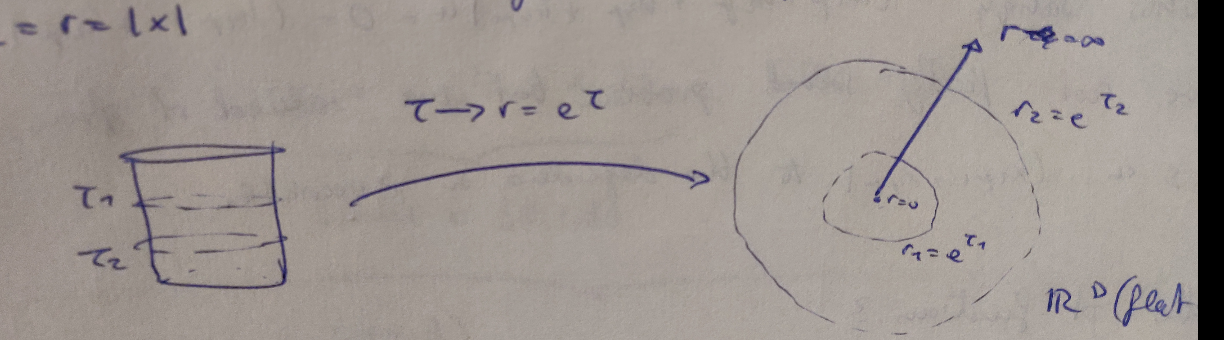
\includegraphics[width=0.63\linewidth]{gfx/Radialquantization}
	\caption{}
	\label{fig:radialquantization}
\end{figure}
Under this conformal transformation from the cylinder to flat space, we have the following $1-1$ mapping of characteristics
\bse 
 \begin{tabular}{|lll|}
 	$\mR \times S^{D-1}$ cylinder & \longrightarrow & $\mR^D$ flat space \\
	\toprule
	$\tau = -\infty$ &&$r=0$\\
	Equal time slice $\tau =\tau_1$ && Equal radius slice $r=r_1$ \\
	Ordinary (equal time) quantization && Radial quantization \\
	Special role for $\tau$ && Special rule for $r$ \\
	Time ordering && Radial ordering ($x^\mu = r n^\mu$) \\
	Time translation $\frac{\partial}{\partial t}$ && Dilatations $\frac{\partial}{\partial \ln r} = r \partial_r = x^\mu \frac{\partial}{\partial x^\mu}$ \\
	Energy of a state && Dilatation weight \\
	Scalar primary operator $\mO_{cyl}(\tau,\vec{n})$ && $\mO_{flat}(r,\vec{n}) = \mO_{cyl} (\tau,\vec{n}) \frac{1}{r^\Delta}$\\
\bottomrule 
\end{tabular}
\ese 
Comparing the hermitian conjugate on both spaces, we note that on the cylinder we have
\bse 
\mO_{cyl} (\tau,\vec{n})^\dagger = \mO_{cyl} (-\tau,\vec{n}).
\ese 
On flat space (upon radial quantization) we have 
\be 
\label{eq:cftRadialQuantizationHermitianConjugate}
\mO^\dagger_{flat}(r,\vec{n}) = \frac{1}{r^{2 \Delta}} \mO_{flat}(\frac{1}{r}, \vec{n}),
\ee 
which is equal to an inversion $I$ acting on $\mO_{flat}$. We can deduce that 
\bse 
(K^\mu)^\dagger = I K^\mu I = P^\mu
\ese 
in radial quantization.

\subsubsection{Operator-state correspondence}
\begin{mybox}{Operator-state correspondence idea}
	In CFT, there is a one-to-one correspondence between states $\ket{\psi}\in \mH$ and local operators acting on $\mH$.
\end{mybox}
\todo{Look at Tong's notes for a more in-depth discussion}
What follows is a sketch or motivation of why that is so.\\
First consider states in QM, i.e. $1$ particle in $1$ spatial dimension. States are equivalent to solutions of the Schrödinger equation, i.e. to Schrödinger-wave functions $\psi(x,t_0)$ at time $t_0$. An initial state is obtained for
\bse 
\psi_{I} (x) = \lim_{t_0\rightarrow - \infty} \psi(x,t_0).
\ese 
We can also consider wave functions in QFT (for simplicity we consider a single scalar particle). Then
\bse 
 \begin{tabular}{|lll|}
	QM & \longrightarrow & QFT \\
	\toprule
Configuration space $x$ && $\phi(x)$ space of fields fixed at $t_0$ \\
Initial state $\psi_I(x)$ && $\lim_{t_0\rightarrow -\infty} \Psi\left[\phi(x,t_0),t_0\right]$ on spatial slices at $t_0$.\\
	\bottomrule 
\end{tabular}
\ese 
What is this functional ?
\bse 
\lim_{t_0\rightarrow -\infty} \Psi\left[\phi(x,t_0),t_0\right]\stackrel{\text{radial quant.}}{\rightarrow} \lim_{r\rightarrow0} \Psi\left[\phi(r,\vec{n}),r\right] 
\ese 
becomes a functional of $\phi(\vec{x})$ at $\vec{x}=0$ upon radial quantization. Thus, $\Psi$ is a function of $\phi(0),\partial_\mu \phi(0),$ $\partial_\mu \partial_\nu \phi(0)$, \dots, which are equivalent to the initial state as it is evaluated at $t_0\rightarrow -\infty$. This is exactly the definition of a local operator, i.e. the space of such functions at $\vec{x}=0$ is the local operator. This is because $t_0 \rightarrow -\infty$ becomes a point (i.e. local) upon radial quantization.\\
In practice, we can label our states via the corresponding operator $\ket{\mO}$ where 
\bse 
\ket{\mO}:= \mO(0) \ket{0},\quad e.g. \hat{ \mI} \leftrightarrow \ket{0}\equiv \ket{\mI}.
\ese
\marginpar{As we are looking at CFT, there is no distinction between interacting and free vacuum. This should therefore be the full vacuum}
What about a state inserting an operator at a different point, e.g. $\mO(x) \ket{0} = \ket{\psi}$ ?
\begin{align*}
\mO(x) & = \mO(0) + x^\mu \partial_\mu \mO(0) + \half x^\mu x^\nu \partial_\mu \partial_\nu \mO(0) + \dots \\
\Rightarrow \quad \ket{\psi}&= \sum_n \frac{1}{n!} x^{\mu_1} \dots x^{\mu_n} \ket{\partial_{\mu_1} \dots \partial_{\mu_n} \mO}.
\end{align*}
Note also that 
\bse
\ket{\partial_\mu \mO} =\partial_\mu \mO(0) \ket{0} = [P_\mu,\mO(0)] \ket{0}= P_\mu \mO(0) \ket{0} = P_\mu \ket{\mO}, 
\ese 
where we assumed $P_\mu \ket{0} =0$, this holds for a Poincaré invariant theory.\\
What is this good for ?\\
\begin{mybox}{}
We can think of operators as states. This means that we can label states by the dilatation weight of the corresponding operator.
\end{mybox}
To label states via the dilatation weight, we need to find out how the dilatation operator acts on states?\\
In standard QFT, we label states by their energy (amongst other quantum numbers, e.g. \ref{eq:fockstates}). Here, upon radial quantization we have seen that energy becomes the dilatation weight\footnote{this comes about a dilatation on the cylinder is a translation in time, as it is radial scaling flat space, and time translation invariance is connected to energy conservation.}\\
Consider a state $\ket{\mO_\Delta}$ where $\mO_\Delta$ is an operator (primary or descendant) with weight $\Delta$, then
\be 
\label{eq:cftStatesLabelling}
\hat{D} \ket{\mO_\Delta} =\left[[\hat{ D}, \hat{ \mO}_\Delta(0)]+\hat{\mO}_\Delta(0) \hat{D} \right]\ket{0} = \Delta \hat{\mO}_\Delta(0) \ket{0} = \Delta \ket{\mO_\Delta},
\ee 
where we used that $\hat{D} \ket{0} =0$ and that
\bse 
[\hat{D},\hat{\mO}_\Delta (0)]= - \delta_D \hat{\mO}_\Delta(0) = (\Delta + x^\mu \partial_\mu) \hat{\mO}_\Delta |_{x=0} = \Delta \hat{\mO}_\Delta(0).
\ese 
What about descendants ?\\
Consider $P^\mu \ket{\mO_\Delta}=\ket{\partial_\mu \mO_\Delta}$ 
\bse 
\hat{D} \hat{P}^\mu \ket{\mO_\Delta} = [\hat{D}, \hat{P}^\mu] \ket{\mO_\Delta}  + \hat{P}^\mu \hat{D}^\mu \ket{\mO_\Delta} = \hat{P}^\mu \ket{\mO_\Delta} + \Delta \hat{P}^\mu \ket{\mO_\Delta},
\ese
which implies
\be 
\label{eq:cftStatesLadderUp}
\hat{D} \ket{\hat{P} \hat{\mO}_\Delta} = (\Delta +1) \ket{P^\mu \mO_\Delta}
\ee 
whose dilatation weight has been raised by one, the four-momentum is therefore similar to the \emph{creator} ladder operator.\footnote{There is a subtlety happening here operators act other way around in QFT than what we are used to. The quantum operators are different to the corresponding differential operators ito. $[\hat{A},\hat{B}]\mO= - [A,B] \mO$.}
Similarly, $K^\mu$ is a lowering operator.
\begin{mybox}{Labelling states}
	$P^\mu$ is a raising operator and $K^\mu$ is a lowering operator with 
	\bse
	\begin{array}{ll}
		\ket{\Delta} \stackrel{P_\mu}{\rightarrow} & \ket{\Delta+1} \stackrel{P_\mu}{\rightarrow} \ket{\Delta+2 } \stackrel{P_\mu}{\rightarrow} \dots \\
		\ket{\Delta} \stackrel{K_\mu}{\leftarrow} & \ket{\Delta+1}\stackrel{K_\mu}{\leftarrow} \ket{\Delta+2} \stackrel{K_\mu}{\leftarrow}\\
	\end{array}
	\ese 
\end{mybox}
Now we can justify the split between primary and descendants. Start with any state and act with $K_\mu$ on it. Keep going until you hit LWS $0$ (since dilatations weights $\Delta\geq 0$). \emph{The state before you reached $0$ corresponds to a primary operator }!\\
\\
N.B.\\
Action of conformal symmetry on $\ket{\hat{ \mO}}$ is with $x=0$ and thus 
	\bse 
	\delta_D = - \Delta, \; \delta_{K_\mu}=0, \; \delta_{P_\mu} = - \partial \mu
	\ese 
	just given by
	\be 
	K_\mu \ket{\mO} = 0
	\ee 
	if $\mO$ is primary.
 
 
 \subsection{Correlators again, but under the aspect of operator-state correspondence}
 \subsubsection{Two-point functions}
 Note that \emph{two-point functions are equivalent to the overlap of (wavefunction) of two states}. With hermitian conjugation upon radial quantization \ref{eq:cftRadialQuantizationHermitianConjugate} we have with $r_1=u^{-1}$, $r_2=r$
 \bse 
 \braket{\mO_{\Delta_1}}{\mO_{\Delta_2}} = \stackrel{ \lim}{r\rightarrow0, u \rightarrow \infty} u^{2 \Delta_1} \expval{\mO_{\Delta, I}(u,\vec{n}_1) \mO_{\Delta,2}(r,\vec{n}_2) }{0}.
 \ese 
 For $\mO_{\Delta_i}$ primaries, we know that \ref{eq:cftCorrelatorTwoPoint} holds. Making use of one of the limits
 \bse 
(x_1-x_2)^\mu = u \vec{n}^\mu_1 - r \vec{n}^\mu_2 \rightarrow u \vec{n}^\mu_1, \; (x_1-x_2)^2=u^2 \vec{n}^2_1 = u^2
 \ese
 we find that the correlator 
 \be
 \braket{\mO_{\Delta, I}}{\mO_{\Delta,2}} = \lim_{u\rightarrow \infty} \frac{C_{12}}{u^{2 \Delta}} u^{2 \Delta} = C_{12} 
 \ee 
 is just the coefficient of the two-point function.
 One can reconstruct the $x$-dependence for the two-point function by considering the overlap
 \be 
 \expval{e^{-\frac{K\cdot y}{y^2}} e^{P\cdot x}}{\mO_\Delta} = \frac{C_{12}}{\abs{x-y}^{2 \Delta}} 
 \ee 
 which recovers \ref{eq:cftCorrelatorTwoPoint}.
 \subsubsection{Three point function}
 One can deduce that 
 \be 
 \bra{\mO_{\Delta, I}} \mO_{\Delta,2}(\hat{ 1}) \ket{\mO_{\Delta, 3}} = C_{123}, \quad \hat{1} \equiv (1,0,0,\dots).
 \ee 
 
 
 
  \subsection{The Operator Product Expansion OPE}
  \begin{mybox}{OPE}
  	In a CFT, we can write the product of two operators at different points as a sum of operators at one point
 \begin{equation}
 \label{eq:cftOPE}
 \Phi_{\Delta_1}(x) \Phi_{\Delta_2}(0) = \sum_{\text{primary } \mO} C_{\Phi_1 \Phi_2 \mO} C_{\mO}(x,\partial_y) \mO(y) |_{y=0} 
 \end{equation}
 where $C_{\mO}(x,\partial_y)$ should be thought of as a power series in $\partial_y$ generating the descendants (not necessarily scalar, can dependent on different indices).\\
 This is convergent as long as there are no operators between $x$ and $0$.
 \end{mybox}
The proof stems from the operator-state equivalence: You can expand the product of states via the completeness relation to a sum of states, i.e. a sum of operators
\subsubsection{Consequence}
This means that we can reduce an $n$-point function to a $(n-1)$-point function
\bse 
\expval{\mO_1 \dots \mO_n} = \sum_{\mO^\prime} C_{\mO_{n-1} \mO_n \mO^\prime} C_{\mO^\prime} (x,\partial_y) \expval{\mO_1 \dots \mO_{n-2} \mO^\prime}.
\ese 
You can keep going and reduce any $n$-point function down to three-point functions by this, which are then again just given by the OPE coefficients for the three-point function $C_{\Phi_1 \Phi_2 \mO}$ \ref{eq:cftCorrelatorThreePoint}.\\
\\
Note that $C_{\mO}$ is solely kinematical, it only says in which representation $\Phi_1,\Phi_2,\mO$ are given in. $C_{\Phi_1\Phi_2 \mO}$ however depends on the theory, this is the specific data of the theory ! This is why we said initially that you know everything if the three-point functions are known.

\subsubsection{How to compute the generator of descendants}
Focus on the case where $\Phi_{\Delta_1}, \Phi_{\Delta_2},\mO_\Delta$ are all scalar primaries\footnote{Only recently people have started studying cases where external fields are non-scalar, e.g. spinor.} Consider the three-point correlator, which we know up to a constant \ref{eq:cftCorrelatorThreePoint}, and plug it into \ref{eq:cftOPE}
\bse 
\expval{\Phi_1(x) \Phi_2(0) \Phi_3(z)} = \sum_{\mO} C_{\Phi_1 \Phi_2 \mO} C_{\mO} (x,\partial_y) \expval{\mO(y) |_{y=0} \Phi_3(z)}
\ese 
where we know from \ref{eq:cftCorrelatorTwoPoint} that the two-point correlator is only non-vanishing if $\mO = \Phi_3$\footnote{A priori only their weights have to be the same, but we can choose a basis of the space of operators with same weight such that operators are orthogonal if they don't have the same weight, i.e. their respective two-point function vanishes.}
We therefore have that this three-point correlator with \ref{eq:cftCorrelatorTwoPoint} is equivalent to
\be 
\label{eq:cftOPEdescendants}
\frac{C_{\Phi_1 \Phi_2 \Phi_3}}{\abs{x}^{\Delta_1+\Delta_2 -\Delta_3} \abs{z}^{\Delta_2+\Delta_3-\Delta_1} \abs{x-z}^{\Delta_1+\Delta_3-\Delta_2} } 
= C_{\Phi_1 \Phi_2 \Phi_3} C_{\Phi_3}(x,\partial_y) \frac{1}{\abs{y-z}^{2 \Delta_3} } |_{y=0}.
\ee\footnote{As hinted at in previous footnote, you would normally get a vector of two-point functions as you would sum over all operators with the same $\Delta$. Due to our choice of basis, i.e. Gram-Schmidt procedure, we get this particular result.}
Now identifying $C_{\Phi_1 \Phi_2 \Phi_3}$ with the three-point coefficient, this factors out. Expanding boh sides in $x$ allows us to determine $C_{\Delta_3}(x,\partial_y)$ term by term.\\
E.g. for the LO term as $x\rightarrow 0$
\begin{align*}
	LHS &=\abs{x}^{\Delta_1+\Delta_2 -\Delta_3} \abs{z}^{\Delta_2+\Delta_3-\Delta_1} \abs{z}^{\Delta_1+\Delta_3-\Delta_2} \\
	&= \frac{1}{\abs{x}^{\Delta_1 +\Delta_2 -\Delta_3} \abs{z}^{2 \Delta_3} } = RHS \\
	\Leftrightarrow \quad C_{\Delta_3}(x,\partial_y) &= \frac{1}{\abs{x}^{\Delta_1+\Delta_2-\Delta_3} } + \mO(NLO).
\end{align*}




 \subsection{Mode Expansion}
 \todo{Continue}
 

 \section{Conformal Ward-Takahashi identities}
 In this section we will demonstrate the importance and power of the operator product expansion. Our aim is to compute the OPE between the energy momentum tensor and a conformal field. This will also shield ne light on the nature of the energy momentum tensor and of the conformal anomaly.
 \subsection{General Ward-Takahashi identities}
 To set the stage we derive here the Ward-Takahashi identities for a general field QFT, with specilaisizations to CFTs reserved for late ron. Consider therefore a general QFT in $\md$ dimensions defined by the path integral
 \begin{equation}
 Z=\int \mD \phi e^{-S[\phi]}.
 \end{equation}
 Suppose the theory enjoys the global symmetry
 \begin{equation}
 \label{eq:globalsymmetry}
 \phi \rightarrow \phi^\prime = \phi + \epsilon \delta \phi \quad \epsilon=constant.
 \end{equation}
 That is, the classical action transforms as
 \begin{equation}
 S[\phi] \longrightarrow S^\prime [\phi^\prime] = S[\phi].
 \end{equation}
 Suppose furthermore that the symmetry is non-anomalous, i.e. the measure is invariant.
 
 \subsubsection{Quantum version of Noether's theorem}
 We know that a classical continuous symmetry implies the existence of conserved current $\partial_\alpha J^\alpha =0$. The quantum version of this statement is that $\partial_\alpha J^\alpha(x)=0$ holds as an operator equation, i.e. together with arbitrary operator insertions away from $x$ under the path integral. To derive this quantum version of Noether's theorem for a non-anomalous global symmetry, we start as in the classical case by promoting $\epsilon \rightarrow\epsilon(x)$. Now the measure $\mD \phi$ and the action $S[\phi]$ are no longer separately invariant, but the combined change of the partition function due to the transformation of the measure and of the action can only involve terms proportional to $\partial_\alpha \epsilon(x)$. We can use this observation to define the Noether current by parametrising the change in $Z$ as\footnote{The so-defined $J^\alpha$ receives contributions both the classical action $S$ and, in general, from the transformation of the functional measure.}
 \begin{align}
 	Z\rightarrow Z^\prime &= \int \mD \phi^\prime e^{-S[\phi^\prime]} = \int \mD e^{-S[\phi] -\frac{1}{2 \pi} \int J^\alpha \partial_\alpha \epsilon(x)}  \nonumber \\
 	&= \int \mD \phi e^{-S[\phi]} \left(1-\frac{1}{2\pi} \int J^\alpha \partial_\alpha \epsilon(x)\right)\nonumber \\
 	&= \int \mD \phi e^{-S[\phi]} \left(1+\frac{1}{2\pi} \int \partial_\alpha J^\alpha \epsilon(x)\right).
 \end{align}
 On the other hand
 \begin{equation}
 Z=\int \mD \phi e^{-S[\phi]} = \int \mD \phi^\prime e^{-S[\phi^\prime]} = Z^\prime 
 \end{equation}
 because we just changed the integration variable. Note that this is not a contradiction to the statement that the transformation with $\epsilon$ replaced by $\epsilon(x)$ is no longer a symmetry of the theory, because $S[\phi^\prime]$ and the measure $\mD \phi^\prime$ are not invariant independently. Therefore
 \begin{equation}
 \frac{1}{Z} \int \mD \phi e^{-S[\phi]} \partial_\alpha J^\alpha(x) = \langle \partial_\alpha J^\alpha(x)\rangle =0.
 \end{equation}
 To show that this indeed holds as an operator equation in the above sense, we consider the correlator
 \begin{equation}
 \langle \mO_1(x_1) \dots \mO_n(x_n) \rangle = \frac{1}{Z} \int \mD \phi e^{-S[\phi]} \mO_1 (x_1) \dots \mO_n(x_n).
 \end{equation}
 Under the symmetry \ref{eq:globalsymmetry}m a local operator transforms as
 \begin{equation}
 \mO_i \rightarrow \mO_i + \epsilon \delta \mO_i.
 \end{equation}
 We now promote $\epsilon \rightarrow \epsilon(x)$ such that $\epsilon(x)$ vanishes at the insertion of the operators in the correlator, i.e. $\epsilon(x) |_{x=x_i} =0$.
 \todo{Insert picture}
 The same steps as before yield $0=\langle \partial_\alpha J^\alpha(x) \mO_1(x_1) \dots \mO_n(x_n) \rangle$, i.e.
 \begin{mybox}{Quantum Noether current}
 	\begin{equation} 
 	0 = \partial_\alpha J^\alpha \quad \text{as an operator equation}.
 	\end{equation}
 \end{mybox}
 To avoid confusions with what comes next, we hasten to stress that this should really be read as the statement that 
 \begin{equation*}
 	0 = \langle \int_B \partial_\alpha J^\alpha(x) \mO_1 (x_1) \dots \mO_n(x_n) \rangle 
 \end{equation*}
 for an arbitrary region $B$ that does not include any of the operators $\mO_i$.
 
\subsubsection{Ward-Takahashi identities}
Now let $\epsilon(x)$ have support only in a region $B_\epsilon$ that contains the insertion $x_1$ of operator $\mO_1$, but none of the other operators.
\todo{insert picture}
The correlator $\langle \mO_1 \dots \mO_n\rangle$ transforms as
\begin{equation}
\langle \mO_1 \dots \mO_n \rangle \rightarrow \frac{1}{Z} \int \mD \phi e^{-S[\phi]} \left(1+\frac{1}{2\pi} \int_{B_\epsilon } \partial_\alpha J^\alpha \epsilon(x) \right) (\mO_1(x_1) +\epsilon(x_1) \delta \mO_1) \mO_2 \dots \mO_n.
\end{equation}
Let us restrict to $\epsilon$ constant inside $B_\epsilon$. For this we deduce
\begin{equation}
-\frac{1}{2\pi} \langle \int_{B_\epsilon} \partial_\alpha J^\alpha(x) \mO_1(x_1) \dots \rangle = \langle \delta\mO_1(x_1) \dots \rangle,
\end{equation}
i.e.
\begin{mybox}{Ward-Takahashi identity}
	\begin{equation}
	-\frac{1}{2\pi} \int_{B_\epsilon} \partial_\alpha J^\alpha(x) \mO_1(x_1) = \delta \mO_1(x_1) \dots \text{  as an operator equation.}
	\end{equation}
	This is the \emph{Ward-Takahashi identity}, which gives a tool to compute the transformation of a local operator by an integral over a certain operator product.
\end{mybox} 

We finally specialize to a $2d$ QFT, for which the Ward identities can be rewritten in a particularly neat manner. By Stoke's theorem we can evaluate $\int_{B_\epsilon} \partial_\alpha J^\alpha(x)$ as a line integral over the boundary of $B_\epsilon$,
\begin{equation*}
	\int_{B_\epsilon} \partial_\alpha J^\alpha(x)= \oint_{\partial B_\epsilon} J_\alpha \hat{n}^\alpha.
\end{equation*}
The tangential and normal line element in two dimensions take the form
\begin{equation}
\hat{t}^\alpha = \begin{pmatrix}
\md x^1 \\
\md x^2 \\
\end{pmatrix},
\quad 
\hat{n}^\alpha=
\begin{pmatrix}
\md x^2\\
-\md x^1\\
\end{pmatrix}.
\end{equation}
\todo{insert picture } 
Therefore we can write
\begin{equation}
\int_{B_\epsilon } \partial_\alpha J^\alpha(x) = \oint_{\partial B_\epsilon} (J_1 \md x^2 -J_2 \md x^1).
\end{equation}
Let us go to complex coordinates $z=x^1+ix^2$, $\bar{z}=x^1-i x^2$, in which
\begin{align*}
	J^z &= J^1+i J^2,\quad J^{\bar{ z}} = J^1-iJ^2,\\
	J_{\bar{ z}} &= g_{\bar{ z} z} J^z = \half (J_1 +iJ_2), \quad J_z = \half (J_1 -iJ_2)
\end{align*}
and therefore
\begin{equation*}
	\int_{B_\epsilon} \partial_\alpha J^\alpha(x)=-i \oint_{\partial B_\epsilon} (\md z B_z - \md \bar{ z} J_{\bar{ z}}), \; J_z = J_z(z,\bar{ z}), \; J_{\bar{ z}} = J_{\bar{ z}} (z,\bar{ z}).
\end{equation*}
\begin{mybox}{Ward-Takahashi in $\md=2$}
	Altogether the Ward-Takahashi identities for a $2$-dimensional QFT take the form
	\begin{equation}
	\delta \mO(\omega,\bar{\omega}) = - \frac{1}{2 \pi i} \oint_{\partial B_\epsilon} (\md z J_z(z,\bar{ z}) - \md \bar{ z} J_{\bar{ z}} (z,\bar{ z})) \mO(\omega,\bar{\omega}),
	\end{equation}
	where it is important that $\omega$ lies within the region $B_{\epsilon}$, i.e. is encircled by the contour integral.
	\end{mybox}

 	
 	
 	 	
 	\subsection{Conformal Ward identities}
 	\begin{mybox}{}
 		General ward identity
 		\begin{equation}
 		\delta \phi_1 (x_1) = - \frac{1}{2 \pi} \int_{B_\epsilon} \partial_\alpha J^\alpha \phi_1(x_1).
 		\end{equation}
 		Transformation behaviour of any local object (field) under conformal transformations is encoded in the residua of its OPE (operator product expansion ?) with the energy momentum tensor.
 	\end{mybox}
 	
 	
 	
 	
 	
 	
 	

 	
 	
 	
 	\section{Wilson's OPE}
 	\begin{mybox}{}
 		For a complete set of fields of a CFT $\{\phi_i(z,\bar{z})\}$ we define the operator product expansion (OPE) 
 		\begin{equation}
 		\phi_i(x) \phi_j(y) = \sum_k C^k_{ij}(x-y) \phi_k(y)
 		\end{equation}
 		which converges absolutely and exponentially fast if there exists a ball around $\mO_i$ and $\mO_j$ with no other operator inside.
 	\end{mybox}
 	
 	
 	\section{Hilbert space of a CFT in $\md>2$}
 	
 	
 	
 	\section{State-operator Isomorphism}
 	
 	\begin{mybox}{}
 		\begin{equation}
 		\text{Local operators on the boundary }\leftrightarrow \text{ states on the interval}
 		\end{equation}
 		in pathintegral formalism
 		\begin{equation}
 		\Psi_{\mO} [\phi_b] = \int \mD \phi e^{i S[\phi]} \mO(0)|_{\phi(x)=\phi_b(x) \text{ for } x\in b}
 		\end{equation}
 		is Schrödinger wave functional that maps operator $\mO$ to state $\braket{\Omega}{\Psi}$.
 	\end{mybox}
 	
 	
 	
 	
 	\section{Correlation functions of primary fields and CFT data}
 	\begin{mybox}{}
 		Correlator of one primary field is
 		\begin{equation}
 		\langle \phi_i(z) \rangle = \delta_{h_i,0}.
 		\end{equation}
 		Correlator of two primary fields is
 		\begin{equation}
 		\langle \phi_i(z) \phi_j(\omega)\rangle = \delta_{h_i h_j} \frac{\md_{ij}}{(z-\omega)^{2h_i}}.
 		\end{equation}
 		Correlator of three primary fields
 		\begin{equation}
 		\langle \phi_i(z_i)\phi_j(z_j) \phi_k(z_k)\rangle = \frac{\tilde{C}_{ijk}}{(z_i-z_j)^{h_i+h_j-h_k} (z_j-z_k)^{h_j+h_k-h_i} (z_i-z_k)^{h_i+h_k-h_j} }
 		\end{equation}
 		where $\tilde{C}_{ijk}$ is related to the OPE structure constants by $\tilde{C}_{ijk} = C^l_{ij} \md_{lk}$.\\
 		These three equations force very restrictive forms onto correlators of CFTs. The constants
 		\begin{equation}
 		\{h_i,C_{ijk} \}
 		\end{equation}
 		are the \emph{CFT data} and are postulated by Wilson's OPE to completely fix all $n$-point correlators and thereby define a CFT without every referring to an action.
 	\end{mybox}
 	
 	
 	
 	
 	\section{Unitarity of CFT in $\md=2$}
 	\begin{mybox}{}
 		A CFT is called \emph{unitary} if 
 		\begin{equation}
 		L^\dagger_m = L_{-m},
 		\end{equation}
 		which ensures that the Hamiltonian is hermitian and $e^{iH}$ is unitary. Necessary conditions are
 		\begin{align}
 			\text{non-negative central charge } C &\geq 0 \\
 			\text{ non-negative conformal weights } h_i &\geq 0 \text{ for all primaries }\phi_i \\
 			\text{there exists a primary $\phi$ with }h_\phi &=0, \text{ i.e. a vacuum}.
 		\end{align}
 	\end{mybox}
 	
 	\begin{equation}
 	\text{ Unitariy $\Rightarrow$ if $h=0$ then $\phi(z)=$constant.}
 	\end{equation}
 	
 	
 	
 	
 	
 	
 	
 	\section{CFT and scale invariance (Zamolodchikov-Polchinski theorem)}
 	\begin{mybox}{}
 		Any conformally invariant theory is scale invariant.\\
 		Any scale invariant and unitary QFT in $\md=2$ is conformally invariant.
 	\end{mybox}
 	Scale invariance
 	\begin{equation}
 	x \rightarrow \lambda x \; \Leftarrow \quad T^\mu_\mu =0 \quad \Rightarrow \; \beta(\lambda) \equiv 0.
 	\end{equation}
 	The direction (scale invariance) $\Rightarrow T^\mu_\mu=0$ has only been proven in special cases.
 	
 	
 	
 	
 	
 	
\chapter{Supersymmetry}
For $4\md $ SuSY we have the bosonic 
\bse 
L_0 := \text{Poincaré-algebra ($+$ R-symmetry $+$ central $U(1)$}
\ese
and the fermionic
\bse 
L_1 := \text{generators are supercharges }Q^I_\alpha, \bar{Q}_{J\dot{\alpha}} = (Q_\alpha)^\dagger,\; I=1,\dots,N.
\ese 
Bosons live in $L_0$ (lie algebra) and fermions live in $L_1$ (Grassmann algebra), where we have a translation via the supercharge
\bse 
\hat{Q} : L_0 \leftrightarrow L_1.
\ese 
\chapter{String Theory}
Ttring theory is a two dimensional conformally invariant field
theory, but not a quantum field theory in four spacetime dimensions.
\section{Motivation}
\begin{enumerate}
	\item Modern physics is primarily built on three pillars that have held up to experiment time and again:
	\begin{enumerate} 
	\item \textbf{Special relativity} is the framework of choice when describing \emph{fast-moving} objects.
	\item  \textbf{General relativity} prevails in the face of objects so \emph{massive} that they bend spacetime itself.
	\item  \textbf{Quantum mechanics} claims to describe physics down to the \emph{smallest} level.
	\end{enumerate} 
	\item  But what if something is both small \emph{and} fast? To describe such systems, special relativity and
	quantum mechanics were beautifully incorporated into a multiparticle, relativistic framework called
	\textbf{quantum field theory} - the most successful physical theory yet, tested to excruciating precision.
	\item Or, what about systems that are massive yet small (and perhaps fast)? Clearly, for something to be
	both massive and small implies that we are looking at high densities on short length scales where
	gravity becomes important and of a magnitude comparable to the other forces. We are entering
	an exotic regime of physics involving systems such as the early universe and (rotating) black holes.
	Quantum field theory in its current state is of no use here, as it discards gravity from the outset. In
	fact, no field-theoretic description of gravity has been found that is both strictly local down to the
	smallest level and consistently quantizable, i.e. that results in a renormalizable quantum theory.
	\item As suggested by the Wilsonian interpretation of QFT, a fundamentally new (nonlocal) picture of
	the microscopic degrees of freedom is needed to make headway. This is where \textbf{string theory} comes
	in, whose central axiom is that \emph{the fundamental objects in Nature are one-dimensional rather than
	pointlike}. Combined with the standard kinematics of \textbf{general covariance}\footnote{General covariance is the paradigm that the form of physical laws should be invariant under arbitrary differentiable coordinate transformations. This statement is motivated by the conviction that coordinates do not exist in nature, and are only artificies of our description. Hence, which ones we choose should play no physical role.} and the usual procedure
	of \textbf{quantization}, this simple statement has resulted in an amazingly rich, mathematically intricate
	and conceptually insightful framework. In particular, string theory leads to a unified description of
	all forces, a divergence-free UV completion of QFT, and it recovers Einstein gravity at low energies.
\end{enumerate}
\subsection{Central properties}
\label{subsec:stringProperties}
\begin{enumerate}
	\item There is only \emph{one} free parameter in string theory, the \textbf{string length} $\ell_s$ which (due to current limits
	of high-energy colliders) can take any value in the range
	\bse 
	\text{(Planck length)}\quad 
	10^{ −35} m < \ell_s < 10^{ −19} m
	\quad \text{(TeV scale)}
	\ese 
	This is in stark contrast to GR and QFT where all masses and higher couplings are input parameters
	that have to be taken from experiment. String couplings are given by expectation values of a
	dynamical field, the scalar dilaton $\phi$. That means they can be calculated from within the theory!
	\item String states can be classified into two regimes:
	\begin{enumerate}
	\item  In the \textbf{low-energy limit} of distances much larger than $\ell_s$ , strings appear pointlike. Integrating
	out the massive string tower results in a low-energy effective theory of only the massless excita-
	tions. These are found to model gauge interactions and gravity. Conformal invariance of the field
	theory on the worldsheet requires that to lowest order, gravity obeys the Einstein equations.
	\item  The \textbf{ultraviolet regime} resides at distances of the order of $\ell_s$. The extended nature of the string
	becomes important, rendering the theory nonlocal with important consequences for interactions:
	Sharp vertices at which interactions are localized in space and time no longer exist.\footnote{In point-particle theories, the sharp localization of vertices is responsible for the appearance of divergent amplitudes.} Locally, the
	string always appears free with interactions encoded solely in the global worldsheet topology.
\end{enumerate}
	\item In string perturbation, each loop order (for a given process) contains only a single diagram. By
	contrast, the number of Feynman graphs in QFT grows factorially. Due to a feature called \textbf{duality},
	there is no need to sum over the scattering channels $s, t, u$. They are all the same in string theory.
	\item A string can be open or closed. Open strings generate Yang-Mills theory, closed strings produce
	gravity. Since open strings can close up and vice versa, gravity and Yang-Mills are dynamically
	related. One automatically implies existence of the other, as it must be, to allow for effects such as
	energy stored in an electric field to gravitate itself. This is what is meant with the statement that
	string theory provides a unified description of all forces.
\end{enumerate}


\section{Classical bosonic string}
\subsection{Bosonic string action}
\begin{mybox}{Nambu-Goto action }
	 The \textbf{Nambu-Goto action} of the classical bosonic string spanning the worldsheet $\Sigma$ is defined as
	\be 
	\label{eq:stringNGaction}
	S_{NG}[X]= - T \int_\Sigma \md A.
	\ee 
	$T$ is the string tension and $\md A=\sqrt{-\det(\vec{G})}\md \tau \md \sigma$ is the area element of $\Sigma$ with coordinates $\vec{\xi}=(\xi^0,\xi^1)=(\tau,\sigma)$. The components of the \textbf{pullback} $\vec{G}$ of the ambient space $\eta\munu$ onto $\Sigma$ are 
	\be 
	\label{eq:stringPullback}
	G_{ab}= \frac{\partial X^\mu}{\partial \xi^a} \frac{\partial X_\mu}{\partial \xi^b},\quad  a,b \in \{0,1\}, \; \mu \in \{0,\dots,d-1\}.
	\ee 
	\end{mybox} 
\begin{mybox}{Polyakov action}
	To eliminate the square root in \ref{eq:stringNGaction}, we introduce the \emph{worldsheet metric } $h^{ab}(\tau,\sigma)$ as an auxiliary (symmetric two-tensor) field and define the \emph{Polyakov action} 
	\be 
	\label{eq:stringPaction}
	S_P [X,h] = -\frac{T}{2} \int_\Sigma \md^2 \xi \sqrt{-h} h^{ab} G_{ab},\quad \text{with } h = \det(\vec{h}).
		\ee 
\end{mybox}
The bosonic string field $X^\mu(\tau,\sigma)$ in $G_{ab}$ provides an embedding of the worldsheet into ambient space. $X^\mu$ is a spacetime vector but a scalar on the worldsheet (due to the absence of worldsheet indices). Hence $S_P$ describes $d$ scalar fields $X^\mu$ coupled to the dynamical worldsheet metric $h_{ab}$. 
\begin{enumerate}
\item Since the spacetime coordinates $X^\mu$ of the string are promoted to dynamical fields, spacetime becomes a derived concept. The fundamental object is the field theory on the worldsheet.
\item $S_P$ and $S_{NG}$ are classically equivalent, i.e. upon enforcing the equation of motion for the auxiliary field $h_{ab}$. However, this equivalence does not extend to the quantum level.
\item \ref{eq:stringPaction} is the most general bosonic string action imaginable. $S_P$ could be modified in two ways
\begin{enumerate}
	\item A \emph{cosmological constant term} 
	\bse 
	S_\Lambda = \Lambda \int_\Sigma \md^2 \xi \sqrt{-h}
	\ese 
	could be added, but this would spoil Weyl invariance which will turn out to be vita for consistency of the CFT on the worldsheet.
	\item We might also include an \emph{Einstein-Hilbert term}
	\bse 
	S_{EH} = \frac{\lambda_{EH}}{4 \pi} \int_\Sigma \md^2 \xi \sqrt{-h}\mathcal{R} 
	\ese 
	with $\mathcal{R}$ the Ricci scalar of the worldsheet. But this is a total derivative and hence introduces no new dynamics (corresponding to the fact that two-dimensional gravity is dynamically trivial).
\end{enumerate}
\end{enumerate}
\subsection{Symmetries}
\subsubsection{Symmetries of the Polyakov action}
$S_P$ enjoys several symmetries, where it is important to distinguish between spacetime symmetries in $\mR^{1,\md-1}$ (taken to be flat) and worldsheet symmetries on $\Sigma$ (dynamic). $S_P$ is invariant under 
\begin{enumerate}
	\item $\md$-dimensional \emph{spacetime} \textbf{Poincaré transformations} 
	\bse 
	X^\mu \rightarrow \Lambda^\mu_\nu X^\nu+V^\mu,
	\ese
	with $\Lambda^\mu_\nu$ in the Lorentz group $SO(1,\md-1)$ and $V^\mu \in \mR^{1,\md-1}$ a translation. The associated conserved charges (according to Noether's theorem\ref{subsec:noethersymmetries}) are energy, momentum and angular momentum.
	\item Local \emph{worldsheet}  \textbf{diffeomorphisms} 
	\bse 
	\xi^a \rightarrow \xi^a + \epsilon^a (\xi)
	\ese 
	under which the string field $X^\mu$ transforms as
	\bse 
	\delta X^\mu= \epsilon^a\partial_a X^\mu,
	\ese
	 the metric $h_{ab}$ as 
	\bse 
	\delta h_{ab} = \nabla_a \epsilon_b +\nabla_b \epsilon_a,
	\ese 
	and the object $\sqrt{-h}$ as $\delta \sqrt{-h}= \partial_a (\epsilon_a \sqrt{-h})$, i.e. like a scalar density of weight $p=1$.
\item Local \textbf{Weyl transformations} 
\bse 
h_{ab} \rightarrow \Lambda(\vec{\xi}) h_{ab} 
\ese 
parametrized by $\Lambda(\vec{\xi})=e^{\omega(\vec{\xi})}$ with $\omega(\vec{\xi})\in \mR$ for convenient series expansion. This symmetry is special in that it arises only for two-dimensional world\emph{sheets} (as opposed to, say, membranes), making strings generalization of point-particles. This symmetries requires $T^a_a=0$ and is crucial for consistent string quantization. 
\end{enumerate}
\subsubsection{Killing symmetry}
The effect on the metric $h_{ab}$ of certain diffeomorphisms $\epsilon_a$ that fulfill the \text{conformal Killing equation} \ref{eq:ctkilling}
\bse 
P^c_{ab} \epsilon_c = (\vec{P} \vec{\epsilon})_{ab} = 0
\ese 
can be undone by a Weyl rescaling $\Lambda^{-1}$. The linear operator $\vec{P}$ is defined via
\be
\label{eq:stringConformalKilling} 
\delta h_{ab} = \nabla_a \epsilon_b + \nabla_b \epsilon_a = \underbrace{\nabla_a \epsilon_b+\nabla_b \epsilon_a - \nabla^c\epsilon_c h_{ab}}_{P^c_{ab} \epsilon_c} + \underbrace{\nabla^c \epsilon_c}_{\Lambda} h_{ab}.
\ee 
These $\epsilon_a$ are the \emph{conformal Killing vectors}. Every such $\epsilon_a$ yields a conserved current
\be 
J^a_\epsilon = T^{ab}\epsilon_b \quad \text{with} \quad \nabla_a J^a_\epsilon = 0 
\ee 
where the conservation follows from the tracelessness of the energy-momentum tensor. The number of such $\epsilon_a$ is infinite and hence infinitely many conserved currents arise.
\subsubsection{Energy-momentum tensor}
\begin{mybox}{Energy-momentum tensor} 
The energy-momentum tensor is defined as the variation of $S_P$ w.r.t. to the worldsheet metric
\be
\label{eq:stringEMtensor}
T_{ab} = \frac{4 \pi}{\sqrt{-h}} \frac{\delta S_P}{\delta h^{ab}} = - \frac{1}{\alpha^\prime} \left(G_{ab} - \half h_{ab} G^c_c\right).
\ee 
It is traceless $T^a_a=0$ (as a consequence of Weyl invariance), and (for on-shell $X^\mu$) constitutes the conserved current $\nabla^a T_{ab}=0$ w.r.t. local worldsheet diffeomorphisms.
\end{mybox}
The equation of motion 
\bse 
T_{ab}=0
\ese 
for $h_{ab}$ implies
\bse 
G_{ab} = \frac{G^c_c}{2} h_{ab},
\ese 
i.e. on-shell $h_{ab}$ is proportional to the pullback.

\subsection{Gauge-fixing}
On a $D$-dimensional worldmembrane, $h_{ab}$ has $\frac{D}{2}(D+1)$ degrees of freedom, while diffeomorphisms plus Weyl rescalings account for $(D+1)$ parameters. Precisely in $D=2$ do we have equally many transformational parameters as metric degrees of freedom. Two more features exclusive to $D=2$ are that the Riemann-tensor has only one degree of freedom given by the Ricci scalar $\mathcal{R}$
\be 
R_{abcd} = \frac{\mathcal{R}}{2} ( h_{ac} h_{bd} - h_{ad} h_{bc}),
\ee 
and second, that under Weyl rescaling $\Lambda(\vec{\xi}), \mathcal{R}$ transforms as
\bse 
\mathcal{R} \rightarrow \mathcal{R} - \vec{\nabla}^2\Lambda(\vec{\xi}). 
\ese 
Choosing $\Lambda(\vec{\xi})$ such that $\mathcal{R}= \vec{\nabla}^2 \Lambda(\vec{\xi})$ (locally, this is always possible) thus implies
\bse 
R_{abcd}=0 \quad \forall a,b,c,d.
\ese 
This means we can always transform the worldsheet so that locally, it resembles flat space. Once space is flat, we can transform coordinates, i.e. apply a diffeomorphism to bring the metric into Minkowskian shape $h_{ab} = \eta_{ab}$. This procedure of fixing the metric is called (partially) \emph{fixing the gauge}.
\begin{enumerate}
	\item It leaves a large \emph{residual gauge symmetry} generated by the conformal Killing vectors $\vec{\epsilon}$ mentioned above. Since these leave the metric invariant, they still represent an unphysical gauge symmetry in our description even after the metric has been fixed.
	\item Worldsheets may exhibit topological obstructions to fixing the metric globally. In this case there remain parameters in the metric, so-called \emph{moduli}, which cannot be removed by a conformal drescaling and diffeomorphisms. These moduli are the global properties of worldsheets that account for string interaction (mentioned in item $2$ of \ref{subsec:stringProperties}).
\end{enumerate}
\subsubsection{Flat gauge}
In \emph{flat gauge} $h_{ab}=\eta_{ab}$, the Polyakov action reduces to the action of $d$ \emph{free} scalar fields,
\be
\label{eq:stringPactionflatgauge}
S_P[X]= \frac{T}{2} \int_\Sigma \md^2 \xi \left[(\partial_\tau \vec{X})^2 - (\partial_\sigma \vec{X})^2\right].
\ee 
\subsubsection{Lightcone coordinates}
Lightcone coordinates $\xi^\pm = \tau \pm  \sigma$ are convenient, e.g. when treating closed string mode expansions with right- and left-moving modes $\vec{\alpha}^\pm_n$ ( $+$ right-moving, $-$ left-moving). The metric in \emph{lightcone gauge} reads
\bse 
h_{\pm \pm} =0, \; h_{\pm \mp} = - \half, \; \text{i.e. } \vec{h}= 
\begin{pmatrix}
	0& - \half \\
	-\half & 0 \\
\end{pmatrix},
\;
\vec{h}^{-1} = 
\begin{pmatrix}
	0 & -2 \\
	-2 & 0 \\
\end{pmatrix},
\ese 
yielding the line element 
\bse 
\md s^2 = h_{ab} \xi^a \xi^b = - \md \tau^2 + \md \sigma^2 = - \md\xi^+ \md \xi^-. 
\ese 
The Jacobian of the transformation $\begin{pmatrix}
\tau \\
\sigma \\
\end{pmatrix}
\rightarrow \begin{pmatrix}
\xi^+ \\
\xi^- \\
\end{pmatrix}
= 
\begin{pmatrix}
\tau + \sigma \\
\tau - \sigma \\
\end{pmatrix}
$ from worldsheet to lightcone coordinates has determinant
\bse 
\abs{\det(\vec{J})} = \abs{\det\begin{pmatrix}
		\partial_\tau \xi^+ & \partial_\sigma \xi^+ \\
		\partial_\tau \xi^- & \partial_\sigma \xi^- \\
\end{pmatrix}}
 = 
 \abs{\det \begin{pmatrix}
 		1 &1 \\
 		1 & -1 \\
 \end{pmatrix}}
=2.
\ese 
Thus the measure becomes 
\bse 
\md^2 \xi = \md \tau \md \sigma = \half \md \xi^+ \md \xi^-
\ese 
and the partial derivatives are $\partial_\pm = \half (\partial_\tau \pm \partial_\sigma)$.\\
\\
The Polyakov action and energy-momentum tensor in lightcone coordinates read 
\be
\label{eq:stringPactionEMtensorLightcone} 
S_P[X] = T \int_\Sigma \md^2 \xi \partial_+ \vec{X} \cdot \partial_- \vec{X},\quad T_{\pm \pm} = - \frac{1}{\alpha^\prime} \partial_\pm \vec{X} \cdot \partial_\pm \vec{X}.
\ee 
Tracelessness translates into $T_{\pm \mp}=0$, and conservation into $\partial_\mp T_{\pm \pm}=0 \Rightarrow T_{\pm \pm} (\xi^{\pm})$. It is important to remember that in flat gauge, the metric's equation of motion $T_{ab}=0$ still has to be enforced as constraint. Partially fulfilled already by tracelessness, this only amounts to $T_{\pm \pm}=0$.\\
The conformal Killing equation $(\vec{P}\vec{\epsilon})_{ab}=0$ in lightcone gauge, where now $\vec{\epsilon}=(\epsilon_+,\epsilon_-)$, becomes the statement $\partial_\pm \epsilon_\pm=0$. Using $\epsilon^\pm = h^{\pm a} \epsilon_a = h^{\pm \mp} \epsilon_\mp = -2 \epsilon_\mp$, this means
\bse 
\partial_\mp \epsilon^\pm = 0 \quad \Rightarrow \quad \epsilon^\pm = \epsilon^\pm(\xi^\pm),
\ese 
i.e. the $\epsilon^\pm$ are chiral.

\subsection{Mode expansion}
\subsubsection{Equation of motion and mode expansion}
Varying the Polyakov action \ref{eq:stringPaction} w.r.t. the bosonic string field yields the free wave equaton
\be 
\label{eq:stringEomBosonic}
(\partial^2_\tau - \partial^2_\sigma) X^\mu = 0 = \partial_+ \partial_- X^\mu 
\ee 
provided the boundary terms vanish. 
\begin{enumerate}
	\item he closed string has cancelling periodic boundaries.
	\item The open string requires \emph{Neumann} ($\partial_\sigma X^\mu =0$) and/or \emph{Dirichlet} ($\delta X^\mu = 0 = \partial_\tau X^\mu$) boundaries at both ends $\sigma \in \{0,l\}$.
\end{enumerate}
Each has a different mode expansion, e.g. the open NN string expansion is
\be
\label{eq:stringOpenModeExpansion}
X^\mu = x^\mu + \frac{p^\mu \tau}{T l} + i \sqrt{2 \alpha^\prime} \sum_{n\neq 0} \frac{\alpha^\mu_n}{n} e^{-i \frac{\pi}{l} n \tau} \cos(\frac{n\pi \sigma}{l}).
\ee 
\subsubsection{Virasoro algebra}
From 
\bse 
\{X^\mu (\tau,\sigma), \Pi^\nu (\tau,\sigma^\prime) \}_{PB} = \eta^{\mu \nu} \delta(\sigma-\sigma^\prime) \quad \text{with } \Pi^\mu = T\partial_\tau X^\mu,
\ese 
the \emph{Poisson bracket} forthe modes follows as
\bse 
\{\alpha^\mu_m,\alpha^\nu_n \}_{PB} = - i m \eta^{\mu \nu} \delta_{m,-n} 
\ese 
(for both left- and right-movers). Also, 
\bse 
\{x^\mu, p^\nu \}_{PB} = \eta^{\mu \nu}.
\ese
Inserting the $\partial_\pm X^\mu$ that result from \ref{eq:stringEomBosonic} into $T_{\pm \pm}$ from \ref{eq:stringPactionEMtensorLightcone} yields the mode expansion
\be 
\label{eq:stringModeExpansionVirasoro}
T_{\pm \pm} = 4 \alpha^\prime \sum_{m\in\Z} L^\pm_m e^{-i \frac{2\pi}{l} m \xi^\pm} 
\ee 
in terms of the \emph{Virasoro generators} $L_m$ (appeared also in \ref{subsubsec:virasoro}). The equation of motion (or constraint if $h_{ab}$ is fixed) $T_{ab}=0$ thus implies the \emph{Virasoro constraints} 
\be
 \label{eq:stringVirasoroConstraints}
L^\pm_m = 0 \quad \forall m \in \Z.
\ee 
In particular, the \emph{Hamiltonian}, which for the open string reads
\begin{align} 
\label{eq:stringHamiltonianOpenBosonic}
H_{op} &= \frac{\pi}{l} L_0 =\frac{\pi}{l} \half \sum_{n\in\Z} \vec{\alpha}_{-n} \cdot \vec{\alpha}_n \\
&= \frac{\pi}{l} \left(\half \vec{\alpha}^2_0 + \half \sum_{n\neq 0} \vec{\alpha}_{-n} \cdot \vec{\alpha}_n\right)= \frac{\pi}{l} \left(\alpha^\prime \vec{p}^2+ \sum_{n=1}^\infty \vec{\alpha}_{-n} \cdot \vec{\alpha}_n\right), \nonumber
\end{align}
must vanish due to $T_{ab}=0$ which implies the (classical open string) \emph{mass shell condition}
\be 
\label{eq:stringMassShellCondition}
M^2 =- \vec{p}^2 = \frac{1}{\alpha^\prime} \sum_{n=1}^\infty \vec{\alpha}_{-n} \cdot \vec{\alpha}_n = \frac{N}{\alpha^\prime}.
\ee 
For closed strings, 
\bse 
H_{cl} = \frac{2\pi}{l} (L^+_0 + L^-_0) \propto \partial_+ + \partial_- \propto \partial_\tau \stackrel{!}{=} 0
\ese 
implements time reparametrization invariance.




\section{Bosonic string quantization}
There are three popular ways to quantize string theory, each with its own merits and downsides.
\begin{enumerate}
	\item In the (old) \emph{canonical quantization}, the Virasoro constraints \ref{eq:stringVirasoroConstraints} are not implemented until we reach the quantum level. This manifestly retains the Lorentz covariance of the classical theory, but a unitary quantum theory is ensured only in a critical number of spacetime dimensions $d_{crit}$.
	\item \emph{Lightcone quantization} enforces Virasoro constrains already at the classical level, resulting in a manifestly unitary quantum theory, but Lorentz covariance holds only in $d = d_{crit}$.
	\item (Modern) \emph{path-integral quantization} uses the Faddeev-Popov gauge fixing procedure. Criticality becomes equivalent to closure of the BRST algebra, which can occur only in $d=d_{crit}$.
\end{enumerate}
\subsection{Canonical quantization}
\subsubsection{Canonical commutation relations}
Canonical quantization promotes all fields to operators and postulates the replacement $\{\cdot,\cdot \}_{PB}\rightarrow \frac{1}{i} [\cdot,\cdot]$, resulting in the canonical commutation relations

\begin{align*}
	[X^\mu(\tau,\sigma),\Pi^\nu (\tau,\sigma^\prime)] &= i \eta^{\mu \nu} \delta(\sigma-\sigma^\prime),\\
	[\alpha^\mu_m,\alpha^\nu_n] &= m \eta^{\mu \nu} \delta_{m,-n}, \\
	[x^\mu,p^\nu] &= i \eta{ \mu \nu}.
\end{align*}
Reality $X^\mu \in \mR$ at the classical level implies hermiticity $(X^\mu)^\dagger = X^\mu$ at the quantum level which in turn requires $(\alpha^\mu_m)^\dagger=\alpha^\mu_{-m}$. This carries over to the Virasoro generators $L^\dagger_m= L_{-m}$.

\subsubsection{Normal ordering}
As always, this procedure is terribly ambiguous because there is nothing to tell us the ’correct’ order within products of noncommuting operators. Hence we simply \emph{define} the \textbf{normal ordering} to be 
\be 
N(\alpha^\mu_m \alpha^\nu_n) = \left\{ \begin{array}{ll}
\alpha^\mu_m \alpha^\nu_n & \text{for } m\leq n,\\
\alpha^\nu_n \alpha^\mu_m & \text{for } n< m,\\
\end{array}\right\}
\ee 
and use this prescription to promote the Virasoro generators to the quantum theory as the operators
\be 
\label{eq:stringVirasorogenerators}
L_m = \half \sum_{n\in \Z} N({\vec{\alpha}}_{m-n} \cdot {\vec{\alpha}}_n).
\ee 
Actual ambiguity arises only in $L_0$ because modes $\alpha^\mu_m,\alpha^\nu_n$ are noncommuting only if $m=-n$ and for $m\neq 0$. By defining $L^{cl}_0 = L^{qu}_0 -a$\footnote{$L^{cl}_0$ and $L^{qu}_0$ are both quantum operators. The superscripts merely indicate that $L^{cl}_0$ has the structure of the classical Virasoro generators without normal-ordering prescription whereas $L^{qu}_0$ does, i.e. is precisely the one defined in \ref{eq:stringVirasorogenerators}.}, where $a$ follows from
\begin{align*}
	L^{cl}_0 &= \half \sum_{n\in\Z} \vec{\alpha}_{-n} \cdot \vec{\alpha}_n = \half \sum_{n=-\infty}^{-1} \left\{\vec{\alpha}_n \cdot \vec{\alpha}_{-n} + \eta\munu \underbrace{[\alpha^\mu_{-n}, \alpha^\nu_n]}_{-n \eta^{\mu \nu}}		\right\} + \half \sum_{n=0}^\infty \vec{\alpha}_{-n} \cdot  \vec{\alpha}_n \\
	&=\half \sum_{n\in\Z} N\left(\vec{\alpha}\cdot \vec{\alpha}_n\right) + \frac{d}{2} \sum_{n=1}^\infty n = L^{qu}_0 -a,
\end{align*}
we capture the ambiguity in a divergent \emph{normal ordering constant} fixed by renormalization later.

\begin{mybox}{Virasoro algebra }
	The \emph{Virasoro algebra} formed by the quantum Virasoro generators 
	\be 
	\label{eq:stringVirasoroAlgebra}
	[L_m,L_n]= (m-n) L_{m+n} + \frac{c}{12} m (m^2-1) \delta_{m,-n}
	\ee 
	is a central extension by $\mC$ of the classical Witt algebra $\{L_m,L_n\}_{PB} = (m-n)L_{m+n}$ satisfied by the classical Virasoro generators. The \emph{central charge} $c = \eta^\mu_\mu = d$ is given by the number of scalars $X^\mu$. The fact that $c \neq 0$ indicates a quantum analogy of the worldsheet's conformal symmetry.
\end{mybox}
To exclude negative norm states from the physical Hilbert space and ensure a unitary theory, we impose (with Ehrenfest's theorem in mind) they \emph{physical state condition} 
\be 
\label{eq:stringPhysicalStatecond}
(L_m-a \delta_{m,0}) \ket{\phi} = 0 \quad \forall m \geq 0 \text{ and } \forall \ket{\phi}\in \mH_{phys}.
\ee 
Since the (quantum) mass shell condition arises from the level-zero Virasoro constraint, the normal ordering constant $a$ affects the string mass. The structure of the physical Hilbert space is a tower of string excitations with increasing mass according to the number of excitations counted by $N$:
\be
M^2_{op} \ket{\phi} = \left(\frac{1}{\alpha^\prime} (N-\alpha) + T^2 \Delta \vec{x}^2\right)\ket{\phi}.
\ee 
$T^2 \nabla \vec{x}^2$ is the energy contribution from the string's tension, non-zero only for states stretched between non-coincident D-branes.The closed string states with $M^2_{cl} \ket{\phi} = \frac{2}{\alpha^\prime} (N^++N^--a) \ket{\phi}$ are oganized by the \emph{level-matching condition}
\bse 
(N^+-N^-) \ket{\phi}=0.
\ese 
\begin{enumerate}
	\item For $a>0$, the vacuum $\ket{0,\vec{p}}$ of bosonic string theory is \emph{tachyonic} with $M^2=-\frac{a}{\alpha^\prime}$. This is not inconsistent, but signals an instability of the (naive) vacuum. Such a theory rapidly decays.
	\item Analysis of the level-zero Virasoro constraint on a first-excited level state
	\bse 
	\ket{\phi} = \xi_\mu \alpha^\mu_{-1}\ket{0,\vec{p}}
	\ese 
	reveals
	\bse 
	(L_0-a)\ket{\phi} = \left(\frac{\vec{\alpha}^2_0}{2}+\vec{\alpha}\cdot \vec{\alpha}_{-1} - a\right)\ket{\phi} = \left(\alpha^\prime \vec{p}^2 +1 -a\right) \ket{\phi}\stackrel{!}{0}
	\ese 
	which implies
	\be
	\vec{p}^2= \frac{a-1}{\alpha^\prime}.
	\ee 
	The level-one constrain evaluates to the requirement of transverse polarization $\vec{\xi}$,
	\bse 
	L_1 \ket{\phi}= \half \left(\dots+ \vec{\alpha}_1 \cdot \vec{\alpha}_0+ \vec{\alpha}_0\cdot \vec{\alpha}_1+\dots\right) \ket{\phi} = \sqrt{2 \alpha^\prime} \vec{p}\cdot \vec{\xi} \ket{\phi} \stackrel{!}{=} 0
	\ese 
	which implies that
	\be 
	\vec{p} \cdot \vec{\xi} =0.
	\ee 
	All higher constraints are vacuous (automatically satisfied). Since for $a>1$ we have $\vec{p}^2>0$, we can choose $\vec{p}$ such that $p^0=0$. Then a purely $\xi^0$-polarized state fulfils $\vec{p}\cdot \vec{\xi}=0$, but, due to 
	\bse 
	\braket{\phi}{\phi} = \bra{0,\vec{p}} (\xi_\mu \alpha^\mu_{-1})^\dagger (\xi_\mu \alpha^\mu_{-1}) \ket{0,\vec{p}} = \xi^\mu \xi_\mu,
	\ese 
	has negative norm for every $\xi^0>0$. Thus $a\leq 1$ is necessary for a unitary quantum theory. For $\ket{\phi}$ twice excited, we similarly find we need $d \leq 26$.
\end{enumerate}

\subsection{Lightcone quantization}
It is convenient in this procedure to introduce lightcone coordinates also for spacetime
\bse 
X^\pm = \frac{1}{\sqrt{2}} (X^0 \pm X^{d-1}), \; X^i, \; i\in \{1,\dots,d-2 \},\; \eta_{\pm \mp} =-1=\eta_{\mp\pm} , \; \eta_{ij}=\delta_{ij},
\ese 
so that $\vec{X}\cdot \vec{X}= -2 X^+ X^- + \sum_i (X^i)^2=- 2 X^+ X^- + \vec{X}^2_\perp$.\\
The key idea of lightcone quantization is to use the infinite dimensional residual symmetry generated by the conformal KIlling vectors fulfilling \ref{eq:stringConformalKilling} to gauge away an infinite number of oscillator derees of freedom, i.e. we set $\alpha^+_n=0 \forall n \neq 0$. This is possible because $\tau = \half (\xi^++\xi^-)$ fulfills the string field's e.o.m. $\partial_+ \partial_- \tau =0$. We can thus find a conformal Killing transformation that reshapes the worldsheet so that its time-axis agrees with one of the spacetime coordinates, say $X^+$, i.e. 
\bse 
X^+ = \frac{2 \pi \alpha^\prime}{l} p^+ \tau + x^+
\ese 
(which is just the mode expansion with all modes except $\alpha^+_0$ set to zero).\\
Of course, this procedure generally breaks Lorentz covariance as it singles out one coordinate!\\
But it enables solving the Virasoro constraints at the classical level. By \ref{eq:stringPactionEMtensorLightcone}, $T_{ab}\stackrel{!}{=}0$ becomes
\bse 
-2 (\partial_\tau \vec{X}\pm \partial_\sigma \vec{X})^+ (\partial_\tau \vec{X} \pm \partial_\sigma \vec{X})^- + (\partial_\tau \vec{X} \pm \partial_\sigma \vec{X})^2_\perp \stackrel{!}{=}0.
\ese 
Inserting the string field expansions turns the Virasoro constraints into an interdependence of modes
\be
\label{eq:stringModesIndependent} 
\alpha^-_n = \frac{1}{\sqrt{2\alpha^\prime} p^+} \half \sum_{i=1}^{d-2} \sum_{m\in\Z} \alpha^i_{n-m} \alpha^i_m.
\ee
Inserting spacetime lightcone coordinates into the flat-gauge Polyakov action from \ref{eq:stringPactionflatgauge} yields
\be 
S_P = \frac{T}{2} \int_\Sigma \md^2 \xi \left[( \partial_\tau \vec{X})^2_\perp - (\partial_\sigma \vec{X})^2_\perp\right] - \int_{-\infty}^{\infty} \md \tau p^+ \partial_\tau q^-.
\ee 
Following the standard quantization procedure gives canonically conjugate variables $X^+ \leftrightarrow \Pi^i$ and $p^+ \leftrightarrow \partial_\tau q^-$ with $q^-= \frac{1}{l} \int_0^l \md \sigma X^-$. Eq. \ref{eq:stringModesIndependent} and $L_m$ quantize as $\alpha^i_{n-m} \alpha^i_m\rightarrow N(\alpha^i_{n-m} \alpha^i_m) - a \delta_{m,0}$.
\\
Since the Virasoro constraints are implemented explicitly, all excitations created by transverse modes $\alpha^i_{-m}$ are automatically physical and the spectrum is manifestly free of ghosts.
\begin{mybox}{}
	\emph{Criticality} in lightcone quantization follows from requiring Lorentz covariance. A long calculation reveals that the \emph{Lorentz algebra} is non-anomalous only if $d=26,a=1$.
\end{mybox}
The quantized Hamiltonian for open NN strings is $H=\frac{\pi}{l}(L_0-a)$. It needs to be \emph{renormalized} due to the divergent $a$. First, we regularize with a cutoff $\Lambda$:
\bse
a= \frac{d-2}{2} \sum_{n=1}^{\infty} n = \lim_{\Lambda \rightarrow \infty} \frac{d-2}{2} \sum_{n=1}^{\infty} n \left(e^{- \frac{\pi}{l \Lambda}} \right)^n.
\ese 
Using $\sum_{n=1}^{\infty} n q^n= q \frac{\md}{\md q} \sum_{n=1}^{\infty} q^n= \frac{q}{(1-q)^2}$, this becomes
\be 
\frac{\pi}{l} a = \lim_{\Lambda \rightarrow \infty} \frac{\pi}{l} \frac{d-2}{2} \frac{e^{-\frac{\pi}{l\Lambda}} }{(1-e^{-\frac{\pi}{l \Lambda}} )^2} = \lim_{\Lambda \rightarrow \infty} \frac{d-2}{2} \left(\frac{l}{\pi} \Lambda^2 - \frac{\pi}{l}\frac{1}{12} +  \mO(\Lambda^{-1}) \right).
\ee 
\begin{enumerate}
	\item The divergent $\Lambda^2$-term scales with $l$. It can be absorbed by adding (via renormalization) a cosmological constant counterterm 
	\bse 
	S_{cc} \propto \Lambda^2 \int_\Sigma \md^2 \xi \sqrt{-h}
	\ese 
	to the bare Polyakov action.\footnote{We have to cancel the divergent term entirely to preserve conformal invariance: A non-zero cosmological constant term would break conformal symmetry already at the classical level. $a\neq 0$ also breaks conformal invariance, but only in the form of an acceptable anomaly at the quantum level.}
	\item The finite term is only present due to the finite size of the string (it disappears for $l\rightarrow \infty$). There exists no local counterterm that could be added to absorb it. This term is therefore physical and define the \emph{Casimir energy} of the string as 
	\bse 
	\frac{\pi}{l} a = \frac{\pi}{l} \frac{d-2}{24}.
	\ese 
\end{enumerate}
For mixed rather than pure NN boundary conditions, the normal ordering constant increases by $\frac{1}{24}$ per $NN-/DD$-dimension and decreases by $-\frac{1}{48}$ per $ND-/DN$-dimension. Thus
\bse 
a_{tot} = \frac{d-2}{24} - \frac{n_{ND}+n_{DN}}{16},
\ese 

\subsection{String spectrum}
\subsubsection{Little group}
In a $d$-dimensional Lorentz covariant theory, states form irreducible representations of the subgroup $\mathbb{S}$ - called \emph{little group} or \emph{stabilizer} - of the $d$-dimensional Poincaré group $SO(1,d-1)\rtimes \mR^{1,d-1}$\footnote{Note that we used the semi-direct product here to construct the Poincaré group.} that leave their momentum $p^\mu$ invariant. Depending on whether $p^\mu$ is space-/light-/timelike, $\mathbb{S}$ is 
\begin{enumerate}
	\item For $\vec{p}^2>0$, we can Lorentz transform to get $\vec{p}=(0,p,0,\dots,0)$ and hence $\mathbb{S}=SO(1,d-2)$. An example is the tachyonic ground state $\ket{0,\vec{p}}$ with $\vec{p}^2= \frac{a}{\alpha^\prime}$, a scalar of the little group $SO(1,24)$.
\end{enumerate}








































\end{document}
% ********************************************************************
